%%%%%%%%%%%%%%%%%%%%%%%%%%%%%%%%%%%%%%%%%%  不使用 authblk 包制作标题  %%%%%%%%%%%%%%%%%%%%%%%%%%%%%%%%%%%%%%%%%%%%%%
%-------------------------------PPT Title-------------------------------------
\title{基于{\rm DFT}的第一原理计算理论与方法导论}
%-----------------------------------------------------------------------------

%----------------------------Author & Date------------------------------------
%\author[\textrm{Jun\_Jiang}]{姜\;\;骏\inst{}} %[]{} (optional, use only with lots of authors)
%% - Give the names in the same order as the appear in the paper.
%% - Use the \inst{?} command only if the authors have different
%%   affiliation.
%\institute[BCC]{\inst{}%
%\institute[Gain~Strong]{\inst{}%
% \vskip -20pt 北京市计算中心}
%\vskip -20pt {\large 格致斯创~科技}}
\date[\today] % (optional, should be abbreviation of conference name)
{%	{\fontsize{6.2pt}{4.2pt}\selectfont{\textcolor{blue}{E-mail:~}\url{jiangjun@bcc.ac.cn}}}
\vskip 45 pt {\fontsize{8.2pt}{6.2pt}\selectfont{%清华大学\;\;物理系% 报告地点
	\vskip 5 pt \textrm{2022-2023}}}
}

%% - Either use conference name or its abbreviation
%% - Not really information to the audience, more for people (including
%%   yourself) who are reading the slides onlin%%   yourself) who are reading the slides onlin%%   yourself) who are reading the slides onlineee
%%%%%%%%%%%%%%%%%%%%%%%%%%%%%%%%%%%%%%%%%%%%%%%%%%%%%%%%%%%%%%%%%%%%%%%%%%%%%%%%%%%%%%%%%%%%%%%%%%%%%%%%%%%%%%%%%%%%%

\subject{}
% This is only inserted into the PDF information catalog. Can be left
% out.
%\maketitle
\frame
{
%	\frametitle{\fontsize{9.5pt}{5.2pt}\selectfont{\textcolor{orange}{“高通量并发式材料计算算法与软件”年度检查}}}
\titlepage
}
%-----------------------------------------------------------------------------

%------------------------------------------------------------------------------列出全文 outline ---------------------------------------------------------------------------------
%\section*{}
%\frame[allowframebreaks]
%{
%  \frametitle{Outline}
%%  \frametitle{\textcolor{mycolor}{\secname}}
%  \tableofcontents%[current,currentsection,currentsubsection]
%}
%%在每个section之前列出全部Outline
%%类似的在每个subsection之前列出全部Outline是\AtBeginSubsection[]
%\AtBeginSection[]
%{
%  \frame<handout:0>%[allowframebreaks]
%  {
%    \frametitle{Outline}
%%全部Outline中,本部分加亮
%    \tableofcontents[current,currentsection]
%  }
%}

%-----------------------------------------------PPT main Body------------------------------------------------------------------------------------
\small
\title{01-量子力学基础}
\section{引言}
\frame
{
	\frametitle{材料模拟的作用与地位}
\begin{figure}[h!]
\vspace*{-0.18in}
\centering
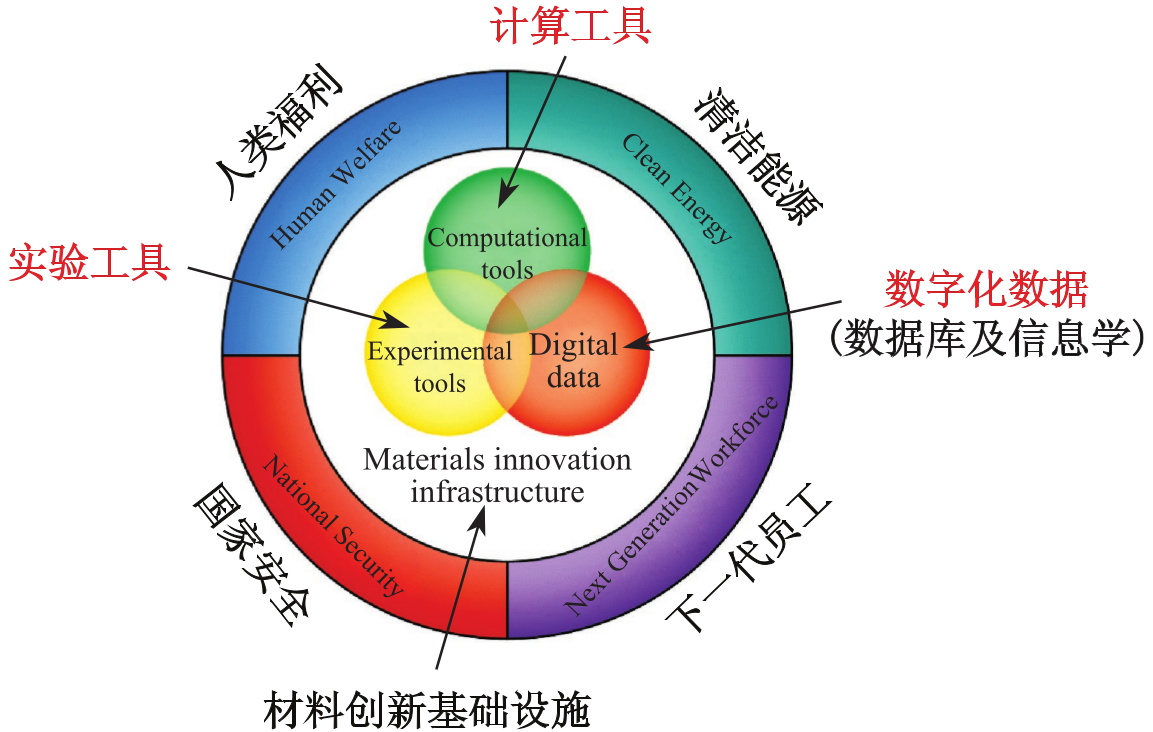
\includegraphics[height=2.55in,width=4.05in]{Figures/MGE.png}
%\caption{\tiny \textrm{Pseudopotential for metallic sodium, based on the empty core model and screened by the Thomas-Fermi dielectric function.}}%(与文献\cite{EPJB33-47_2003}图1对比)
%\caption{\tiny \textrm{Pseudopotential for metallic sodium, based on the empty core model and screened by the Thomas-Fermi dielectric function.}}%(与文献\cite{EPJB33-47_2003}图1对比)
\label{MGE}
\end{figure}
}

\frame
{
	\frametitle{材料模拟的基本思想和方法}
\begin{figure}[h!]
\vspace*{-0.25in}
\centering
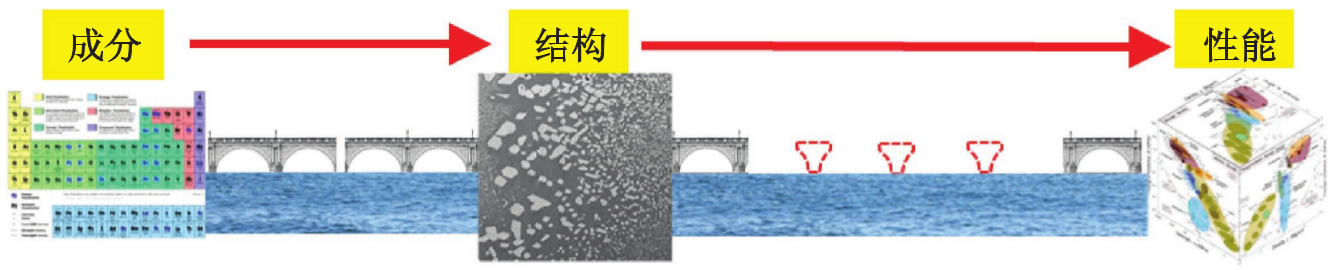
\includegraphics[height=0.80in,width=4.05in]{Figures/MGE-2.png}
%\caption{\tiny \textrm{Pseudopotential for metallic sodium, based on the empty core model and screened by the Thomas-Fermi dielectric function.}}%(与文献\cite{EPJB33-47_2003}图1对比)
\vskip 0.05pt
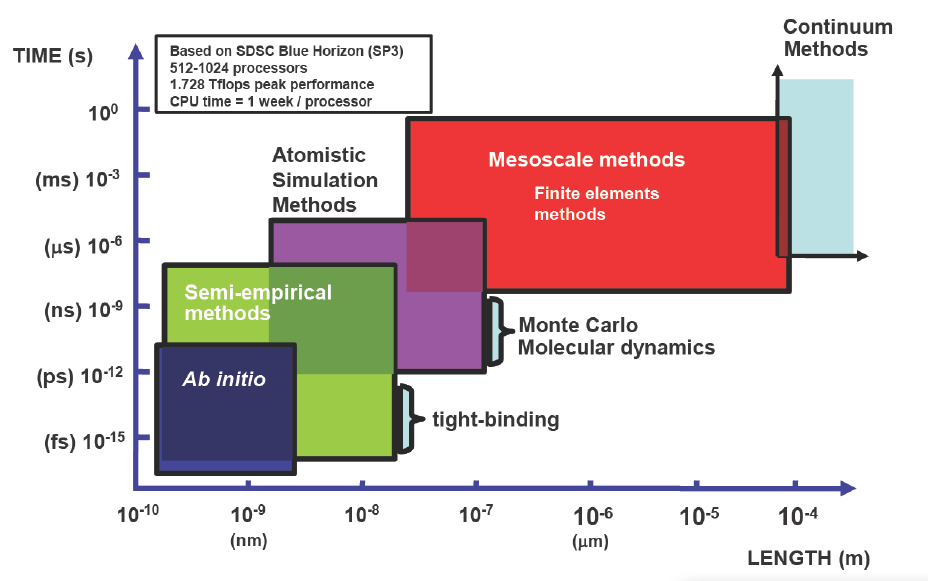
\includegraphics[height=2.20in,width=3.45in]{Figures/Multi-Scale-6.png}
%\caption{\tiny \textrm{Pseudopotential for metallic sodium, based on the empty core model and screened by the Thomas-Fermi dielectric function.}}%(与文献\cite{EPJB33-47_2003}图1对比)
\label{Multi-Scale}
\end{figure}
}

\frame
{
	\frametitle{\rm{I~Have~A~Dream}}
\begin{figure}[h!]
\vspace*{-0.18in}
\centering
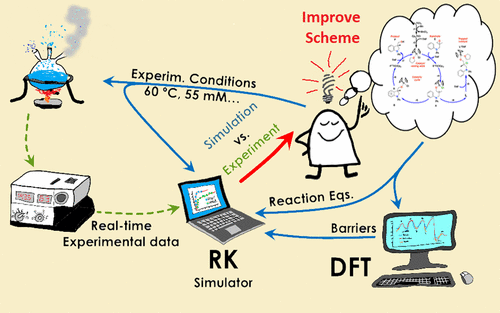
\includegraphics[height=2.55in,width=4.05in]{Figures/Schematic_Material-Design.png}
%\caption{\tiny \textrm{Pseudopotential for metallic sodium, based on the empty core model and screened by the Thomas-Fermi dielectric function.}}%(与文献\cite{EPJB33-47_2003}图1对比)
%\caption{\tiny \textrm{Pseudopotential for metallic sodium, based on the empty core model and screened by the Thomas-Fermi dielectric function.}}%(与文献\cite{EPJB33-47_2003}图1对比)
\label{Schematic_Material-Design}
\end{figure}
}

\section{量子力学基础}
\subsection{能量量子化}
\frame
{
	\frametitle{经典物理学的成功}
\begin{figure}[h!]
\vspace*{-0.18in}
\centering
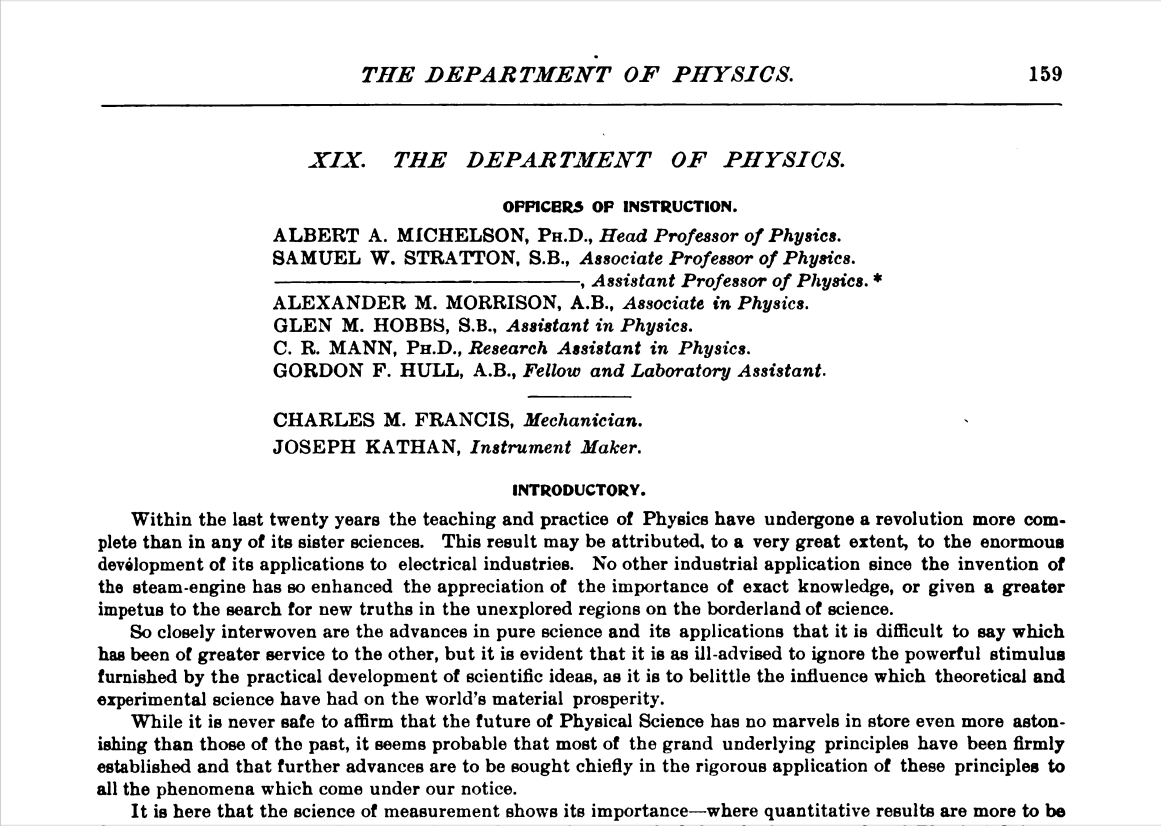
\includegraphics[height=1.90in,width=3.00in,viewport=0 0 1150 690,clip]{Figures/Albert_Michelson-Quotes.jpg}
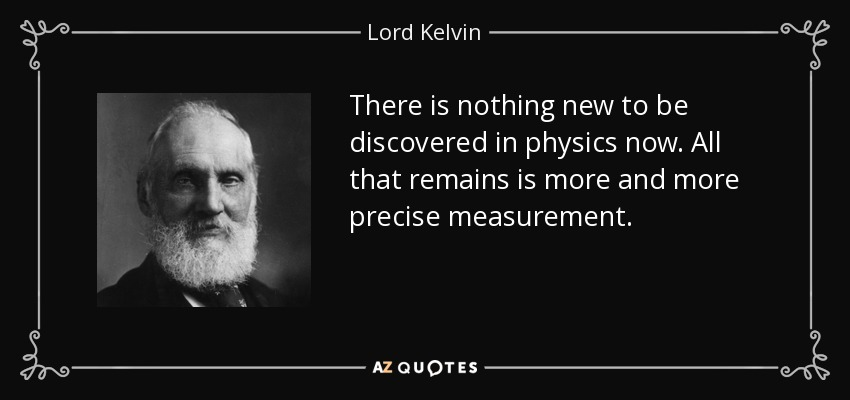
\includegraphics[height=1.10in,width=2.55in,viewport=0 0 880 400,clip]{Figures/Quote-there-is-nothing-new-to-be-discovered-in-physics-now-all-that-remains-is-more-and-more-lord-kelvin-57-38-79.jpg}
%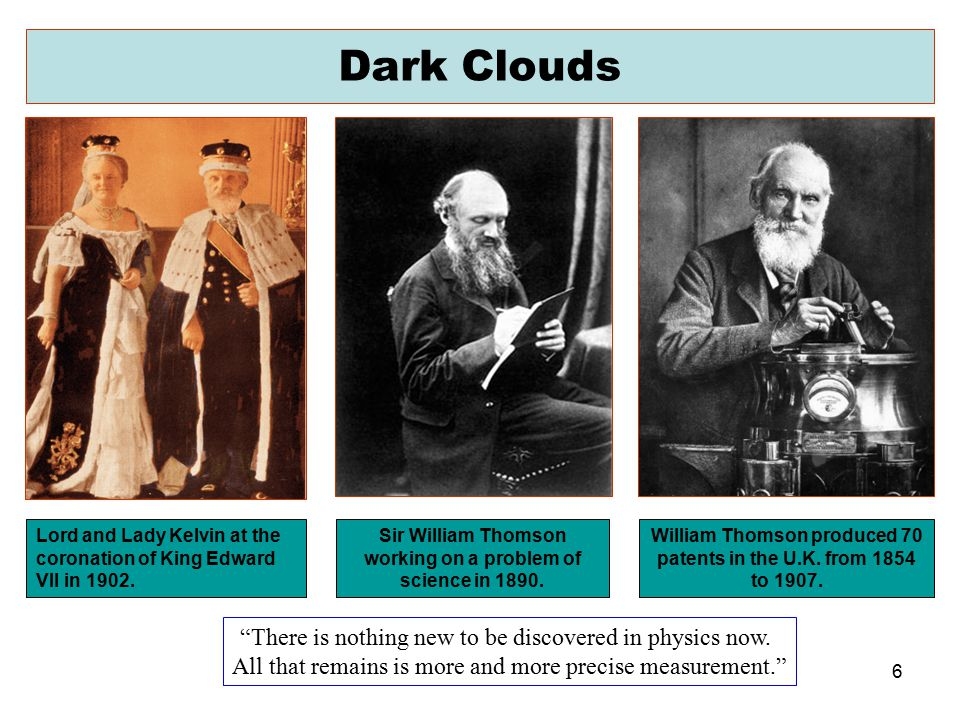
\includegraphics[height=2.50in,width=4.05in,viewport=0 20 735 470,clip]{Figures/Two-dark-cloud-in-physics-3.jpg}
%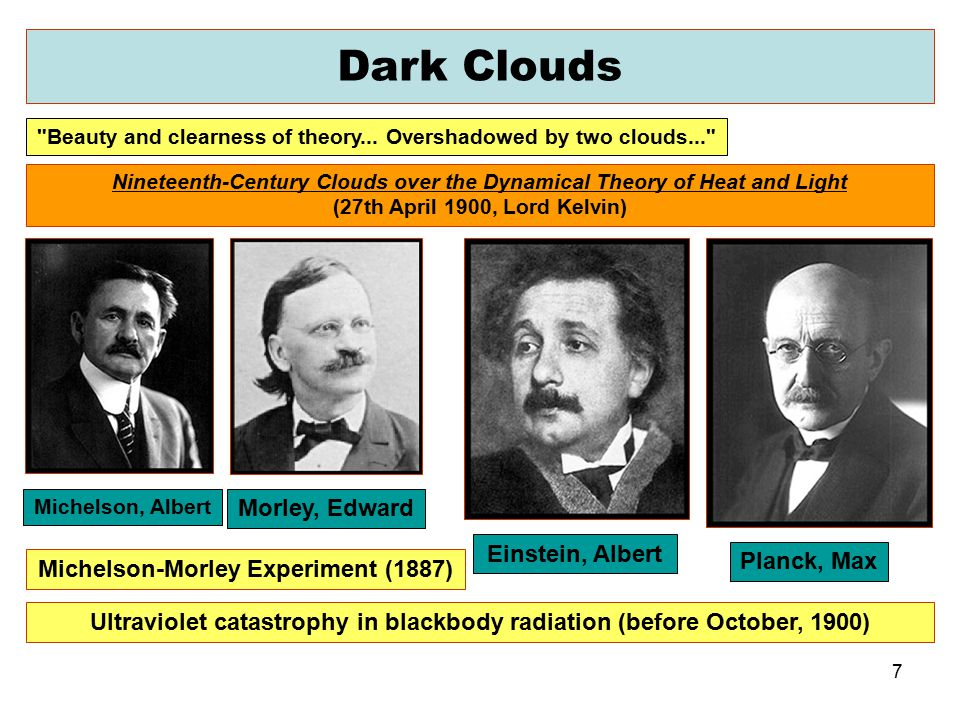
\includegraphics[height=2.40in,width=4.05in,viewport=0 50 735 470,clip]{Figures/Two-dark-cloud-in-physics-2.jpg}
%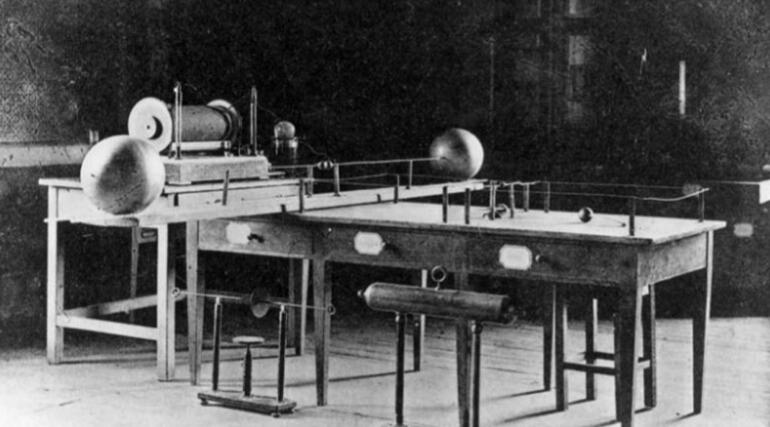
\includegraphics[height=2.40in,width=4.05in,viewport=0 0 580 325,clip]{Figures/Two-dark-cloud-in-physics-1.jpg}
\label{two_Dark_Clouds}
\end{figure}
}

\frame
{
	\frametitle{经典物理学天空的“两朵乌云”\textrm{(Dark Clouds)}}
\begin{figure}[h!]
\vspace*{-0.18in}
\centering
%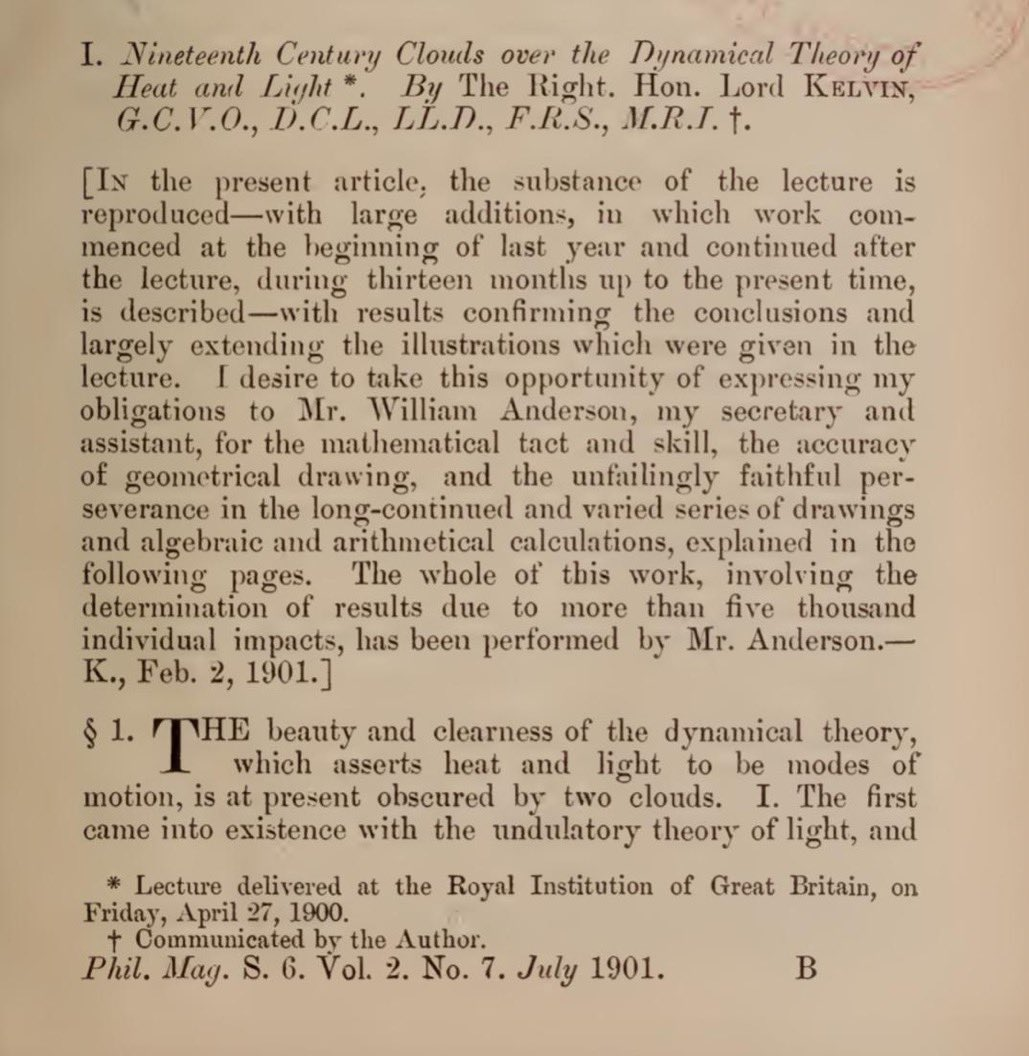
\includegraphics[height=2.90in,width=2.80in,viewport=0 0 1000 1100,clip]{Figures/Baron_Kelvin-Lecture.jpeg}
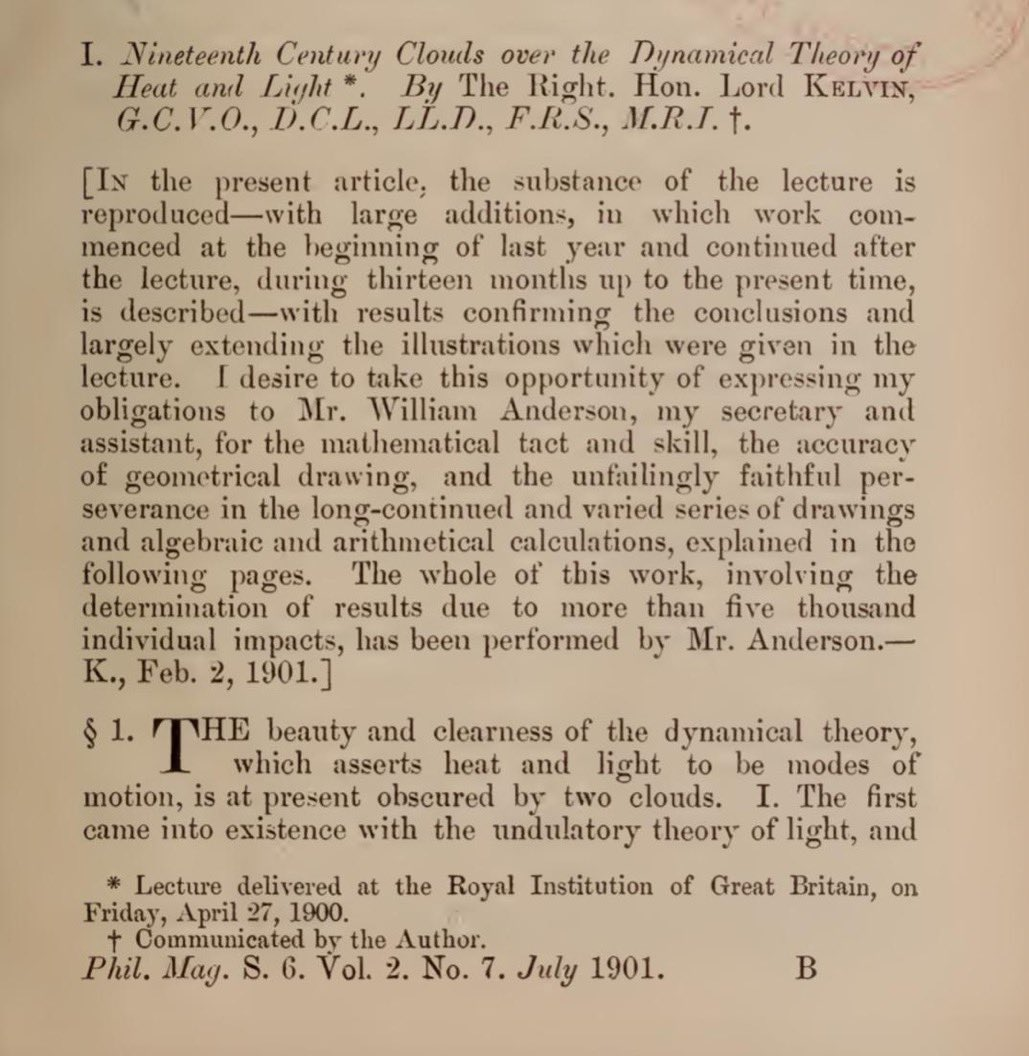
\includegraphics[height=0.35in,width=3.35in,viewport=0 900 1020 1030,clip]{Figures/Baron_Kelvin-Lecture.jpeg}
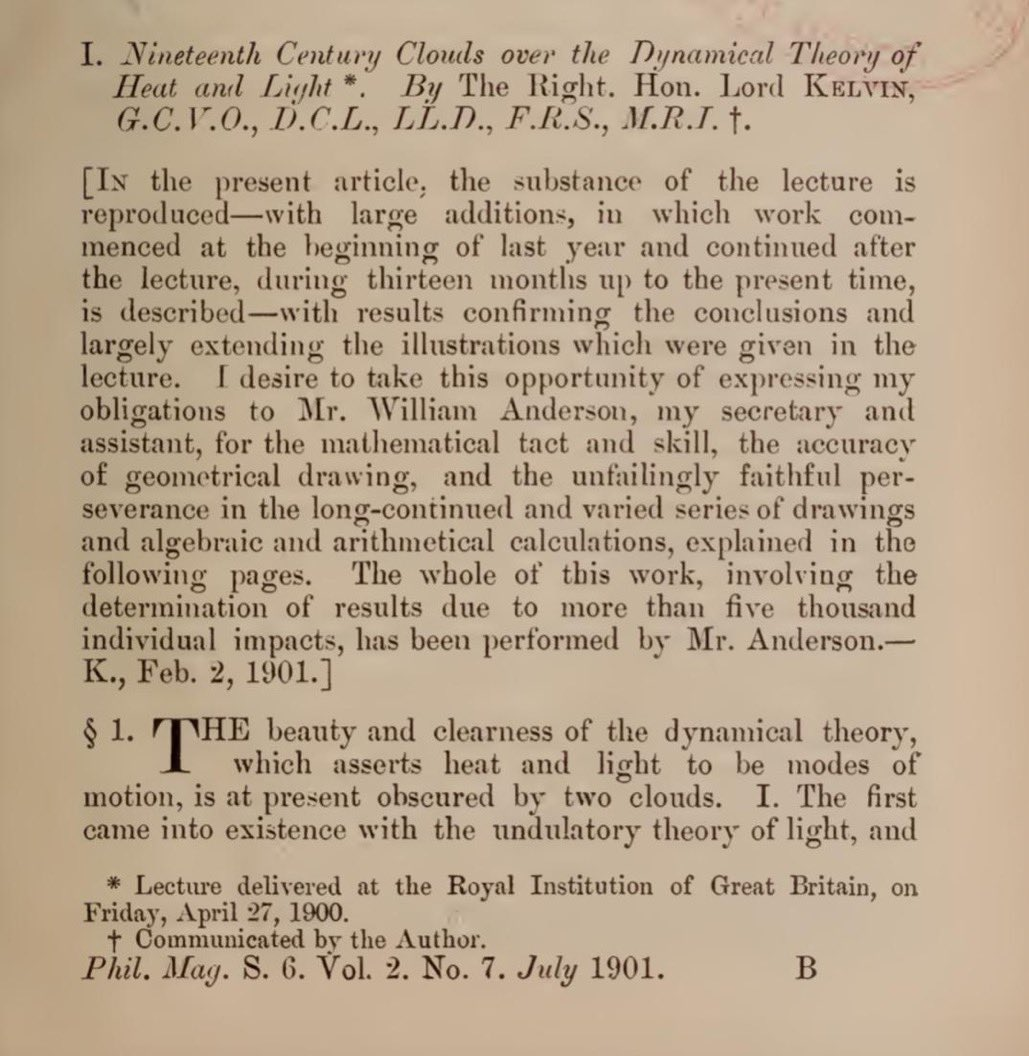
\includegraphics[height=0.80in,width=3.35in,viewport=0 50 1020 350,clip]{Figures/Baron_Kelvin-Lecture.jpeg}
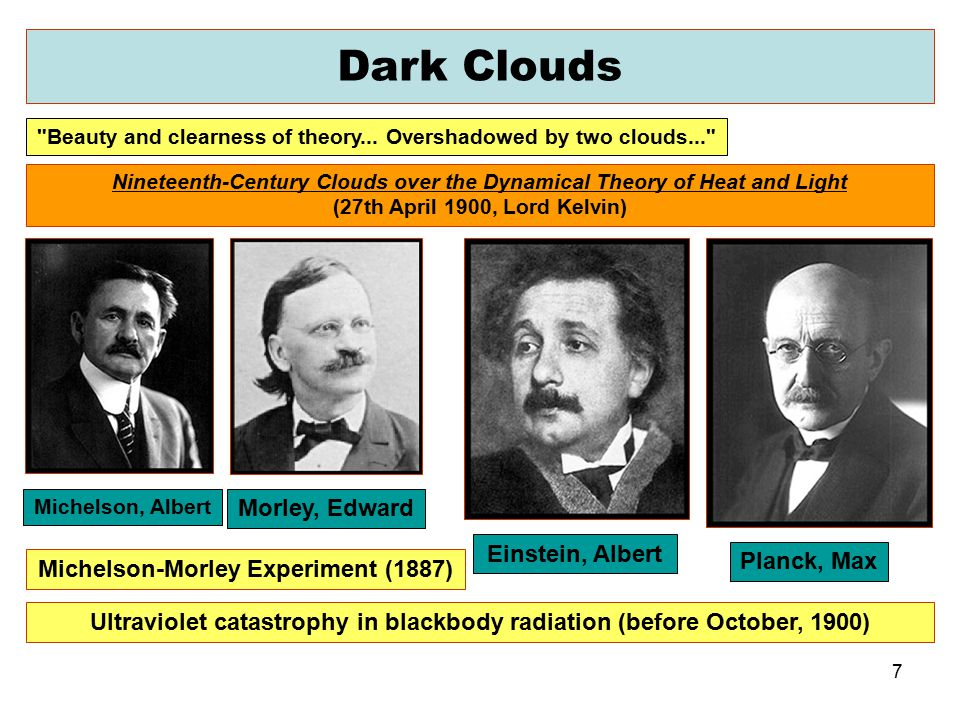
\includegraphics[height=1.85in,width=4.05in,viewport=0 50 735 370,clip]{Figures/Two-dark-cloud-in-physics-2.jpg}
\label{two_Dark_Clouds_2}
\end{figure}
}

%\frame
%{
%	\frametitle{经典物理学天空的“两朵乌云”\textrm{(Dark Clouds)}}
%\begin{figure}[h!]
%\vspace*{-0.18in}
%\centering
%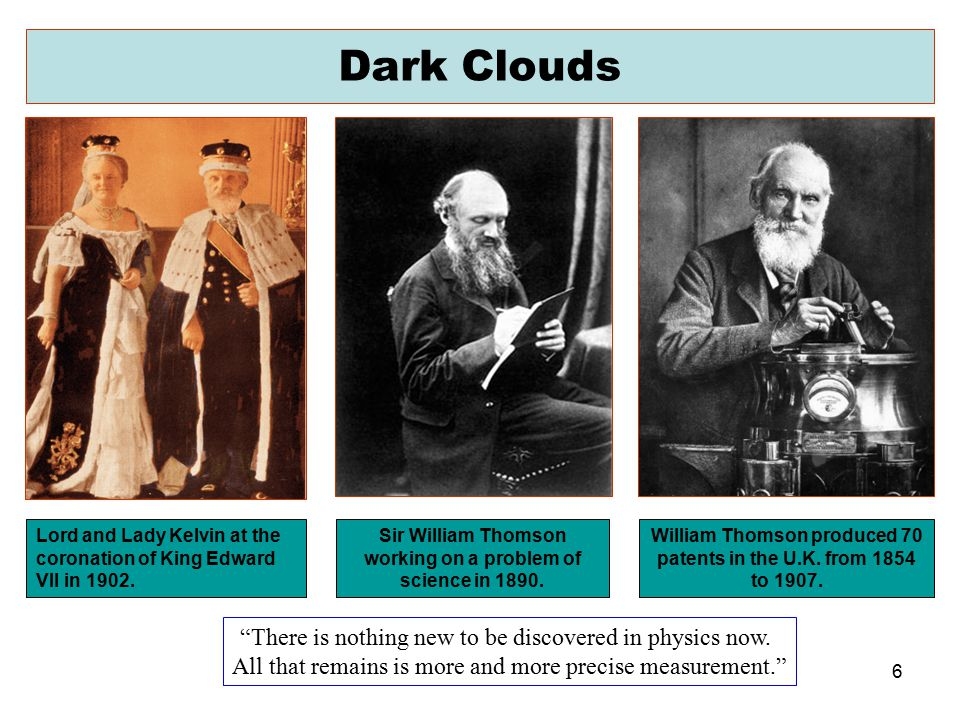
\includegraphics[height=2.50in,width=4.05in,viewport=0 20 735 470,clip]{Figures/Two-dark-cloud-in-physics-3.jpg}
%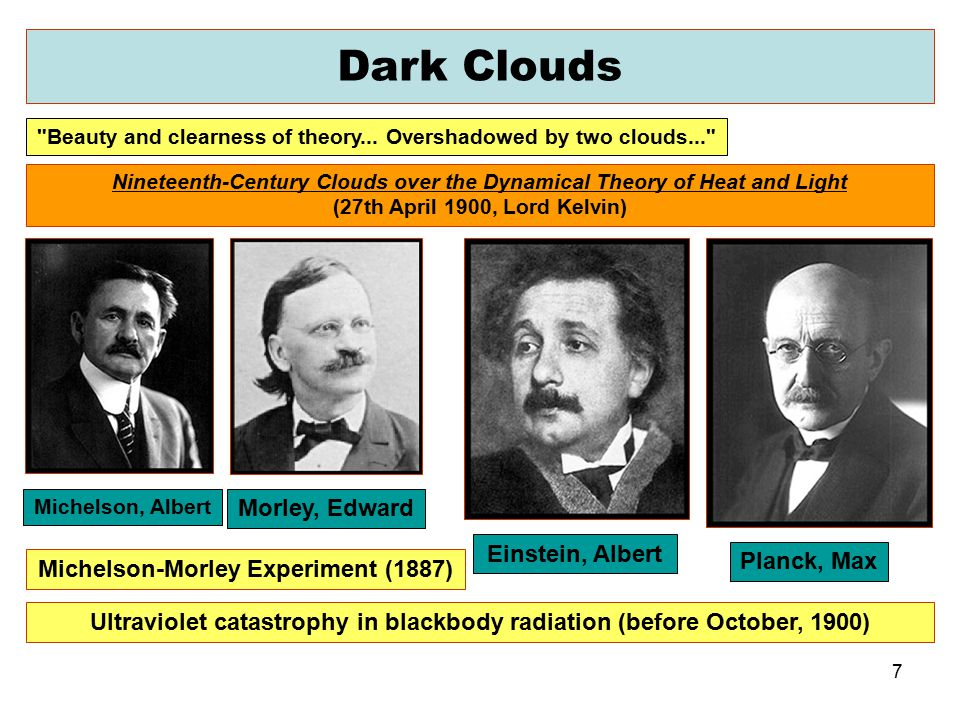
\includegraphics[height=2.40in,width=4.05in,viewport=0 50 735 470,clip]{Figures/Two-dark-cloud-in-physics-2.jpg}
%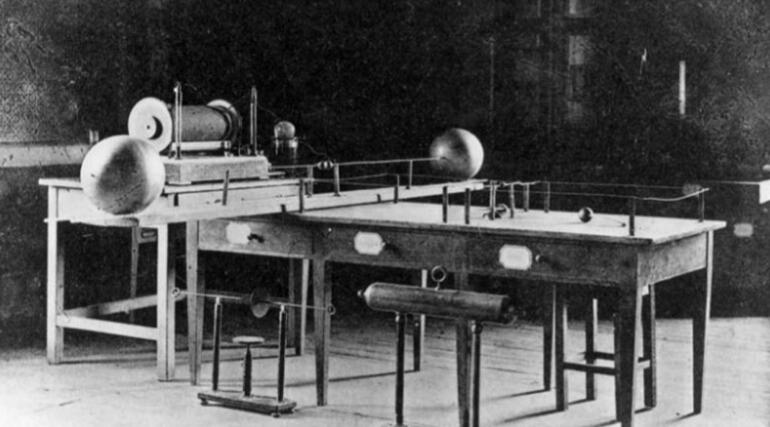
\includegraphics[height=2.40in,width=4.05in,viewport=0 0 580 325,clip]{Figures/Two-dark-cloud-in-physics-1.jpg}
%\label{two_Dark_Clouds_3}
%\end{figure}
%}
%
\frame
{
	\frametitle{黑体辐射与能量量子化}
	\textrm{1900}年,为了解释黑体辐射\textrm{(black-body radiation)}的能量密度与电磁辐射频率的关系,\textrm{M.~Planck}%放弃\textcolor{blue}{能量均分定理}\textrm{(the equipartition theorem)},
	引入\textcolor{red}{能量量子化}\textrm{(quantization of energy)}的假设,利用统计物理推导出与实验符合得非常好的黑体辐射\textrm{Planck~}公式:~
	\begin{displaymath}
		\rho_{\nu}\mathrm{d}{\nu}=\dfrac{8{\pi}h{\nu}^3}{C^2}\bigg(\dfrac1{\mathrm{e}^{h\nu/kT}-1}\bigg)\mathrm{d}\nu
	\end{displaymath}
\begin{figure}[h!]
\centering
\vspace{-10.5pt}
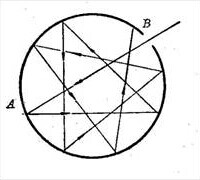
\includegraphics[height=1.45in,width=1.45in,viewport=0 0 136 136,clip]{Figures/Black_box.jpg}
\hskip 1pt
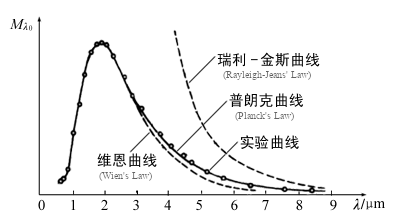
\includegraphics[height=1.32in,width=2.25in,viewport=0 0 390 215,clip]{Figures/Black_box_curve.png}
\caption{\textrm{The black-body radiation and the curve}}
\label{Black_box}
\end{figure}
}

\frame
{
	\frametitle{波-粒二象性与光电效应}
\begin{figure}[h!]
\centering
\vspace{-15.5pt}
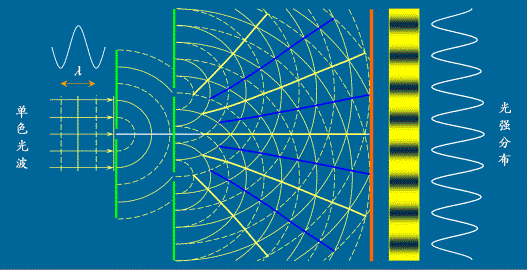
\includegraphics[height=1.35in,width=2.70in,viewport=0 0 536 280,clip]{Figures/wave-particle_duality.png}
\vskip 1pt
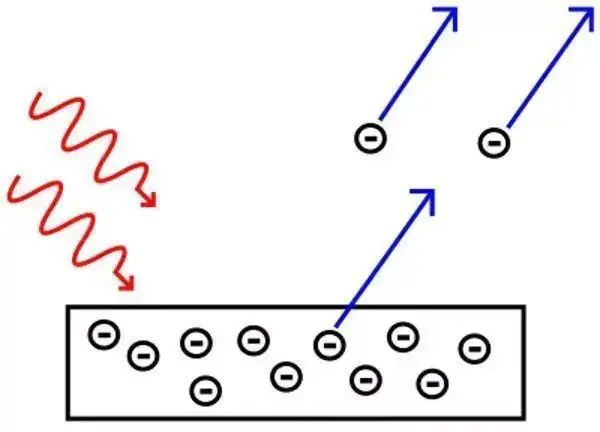
\includegraphics[height=1.32in,width=2.05in,viewport=0 0 620 455,clip]{Figures/Photoelectic_effect.png}
\caption{\textrm{The wave-particle duality and Photoelectric effect}}
\label{wave_and_particle}
\end{figure}
}

\frame
{
	\frametitle{电子衍射、\textrm{Compton~effect}与\textrm{H}原子光谱}
\begin{figure}[h!]
\centering
\vspace{-15.5pt}
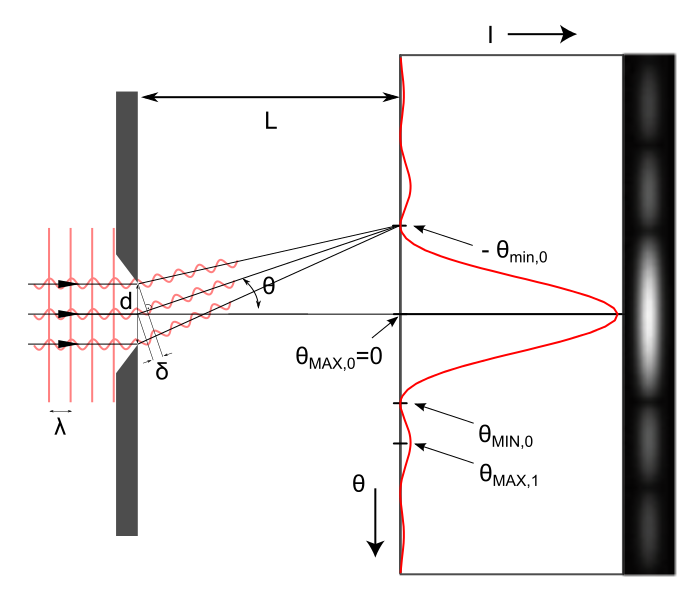
\includegraphics[height=1.35in,width=1.80in,viewport=0 0 680 600,clip]{Figures/Single_Slit_Diffraction.png}
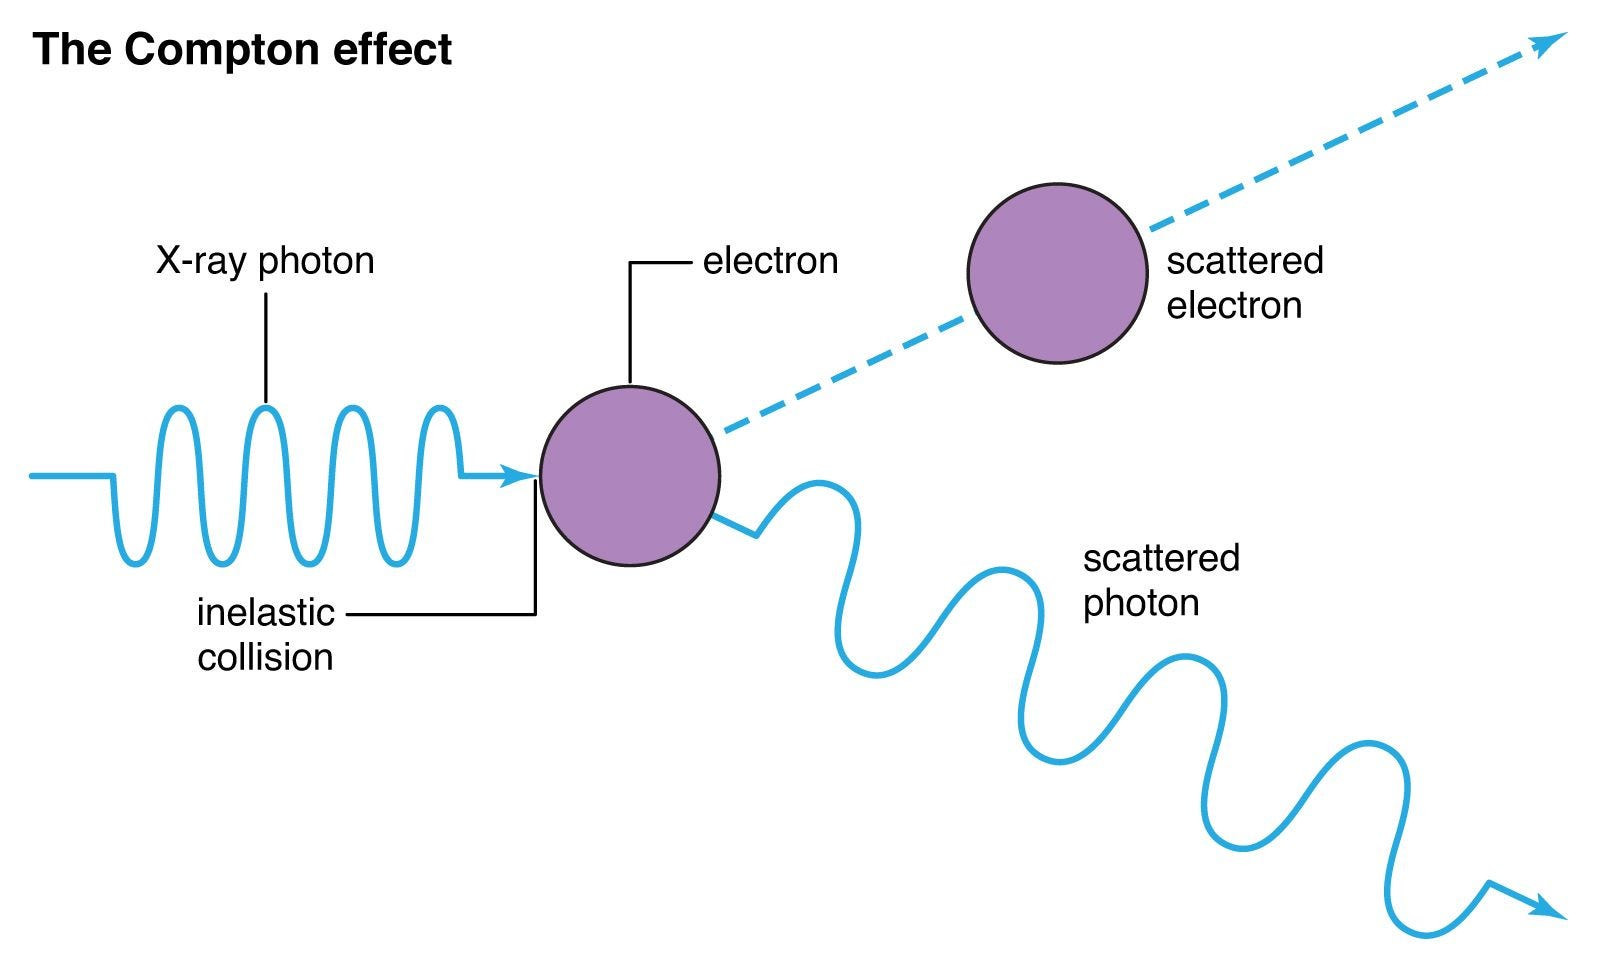
\includegraphics[height=1.20in,width=2.10in,viewport=0 0 1600 950,clip]{Figures/Compton_effect.jpg}\\
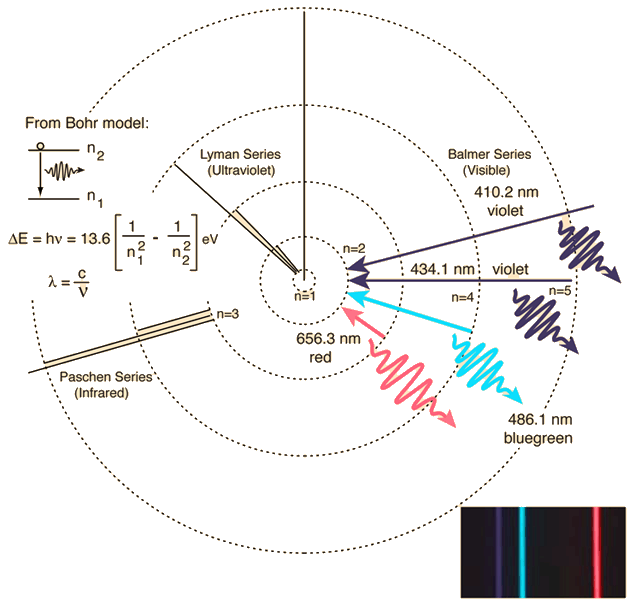
\includegraphics[height=1.65in,width=1.75in,viewport=0 0 620 600,clip]{Figures/Hydrogen_spectrum-3.png}
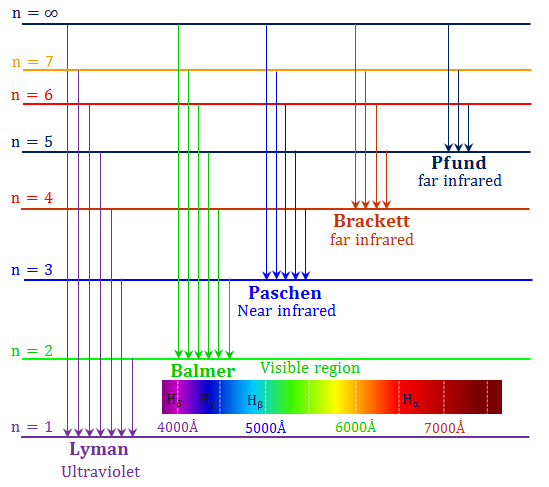
\includegraphics[height=1.55in,width=1.75in,viewport=0 0 500 380,clip]{Figures/Hydrogen_spectrum-2.png}
%\caption{\textrm{The wave-particle duality and Photoelectric effect}}
\label{electron:wave_and_particle}
\end{figure}
}

\subsection{\textrm{Schr\"odinger}方程与量子力学的建立}
\frame
{
	\frametitle{\textrm{De Broglie}物质波}
\begin{minipage}{0.53\textwidth}
\begin{figure}[h!]
\centering
\vspace{-15.5pt}
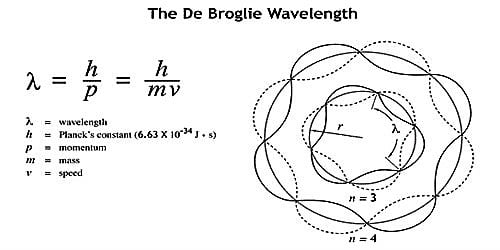
\includegraphics[height=1.3in,width=2.1in,viewport=0 0 500 280,clip]{Figures/De-Broglie-waves.jpg}
%\caption{\textrm{The wave-particle duality and Photoelectric effect}}
\label{Matter_wave}
\end{figure}
经典的观念:
\begin{itemize}
	\item \textcolor{red}{粒子}:~\textcolor{blue}{物质存在的形式}
	\item \textcolor{red}{波动}:~\textcolor{blue}{能量传递的形式}
\end{itemize}
\end{minipage}
\begin{minipage}{0.45\textwidth}
\begin{figure}[h!]
\centering
\vspace{-15.5pt}
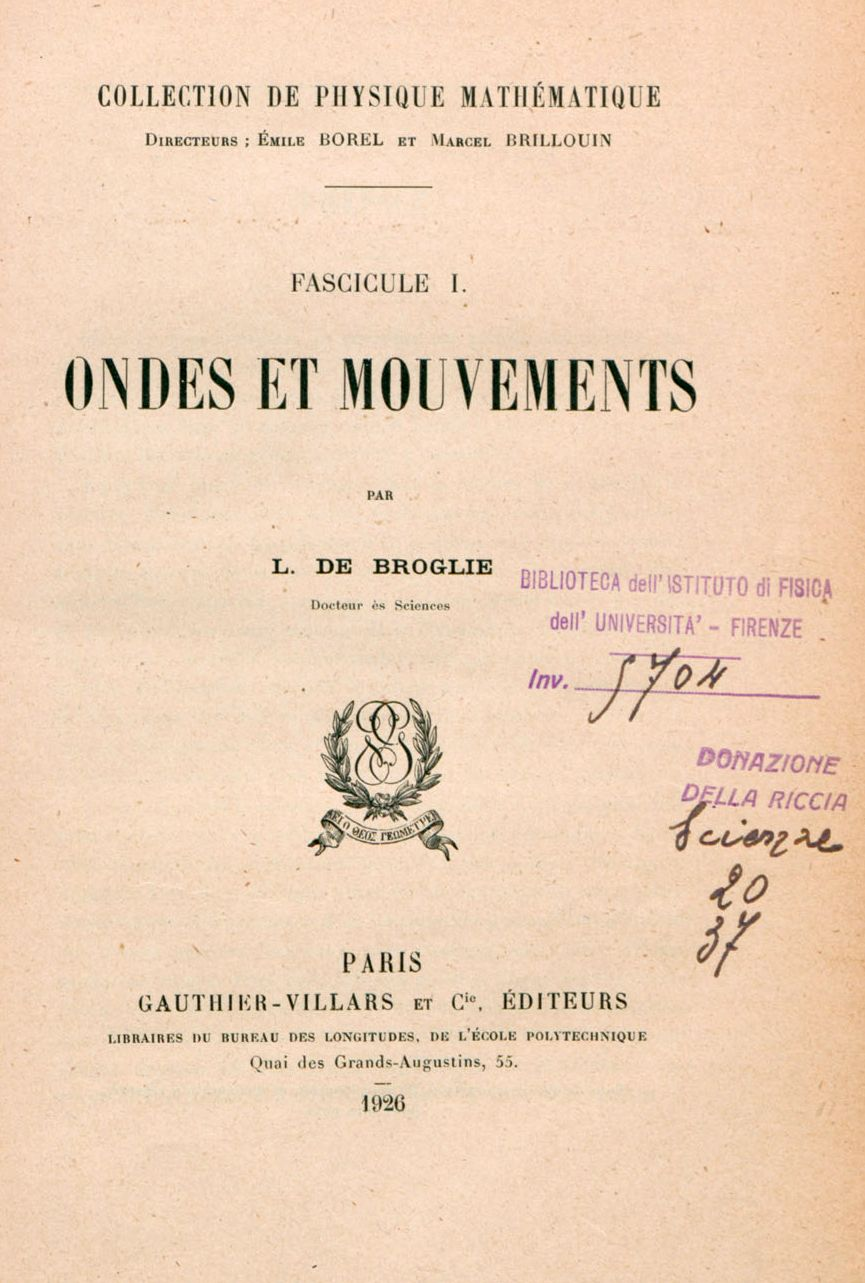
\includegraphics[height=2.80in,width=1.90in,viewport=0 0 430 650,clip]{Figures/De_Broglie-dissertation_Cover.jpg}
%\caption{\textrm{The wave-particle duality and Photoelectric effect}}
\label{De_Broglie-dissertation}
\end{figure}
\end{minipage}
}

\frame
{
	\frametitle{经典力学\textrm{Classical Mechanics}}
\begin{figure}[h!]
\vspace*{-0.18in}
\centering
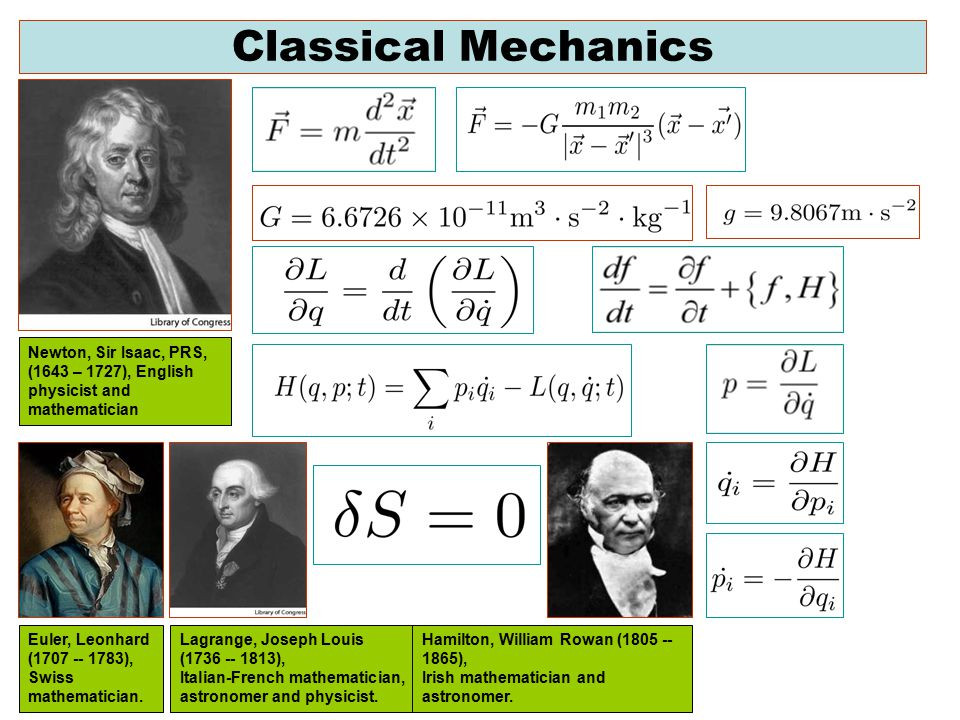
\includegraphics[height=2.65in,width=4.05in,viewport=0 0 715 495,clip]{Figures/Classical_Mechanics.jpg}
%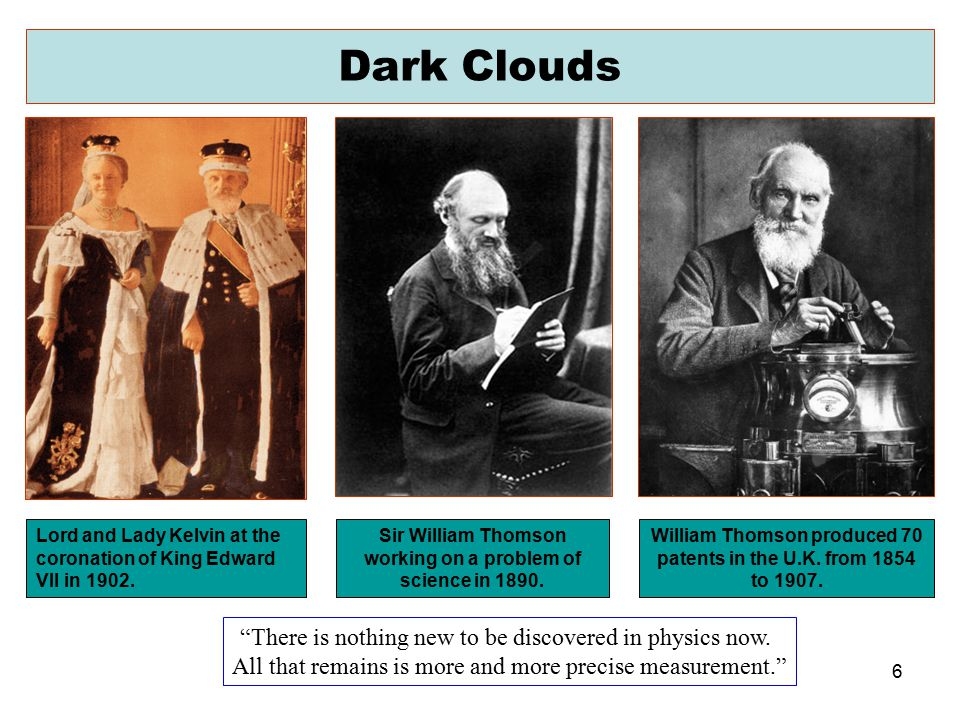
\includegraphics[height=2.50in,width=4.05in,viewport=0 20 735 470,clip]{Figures/Two-dark-cloud-in-physics-3.jpg}
%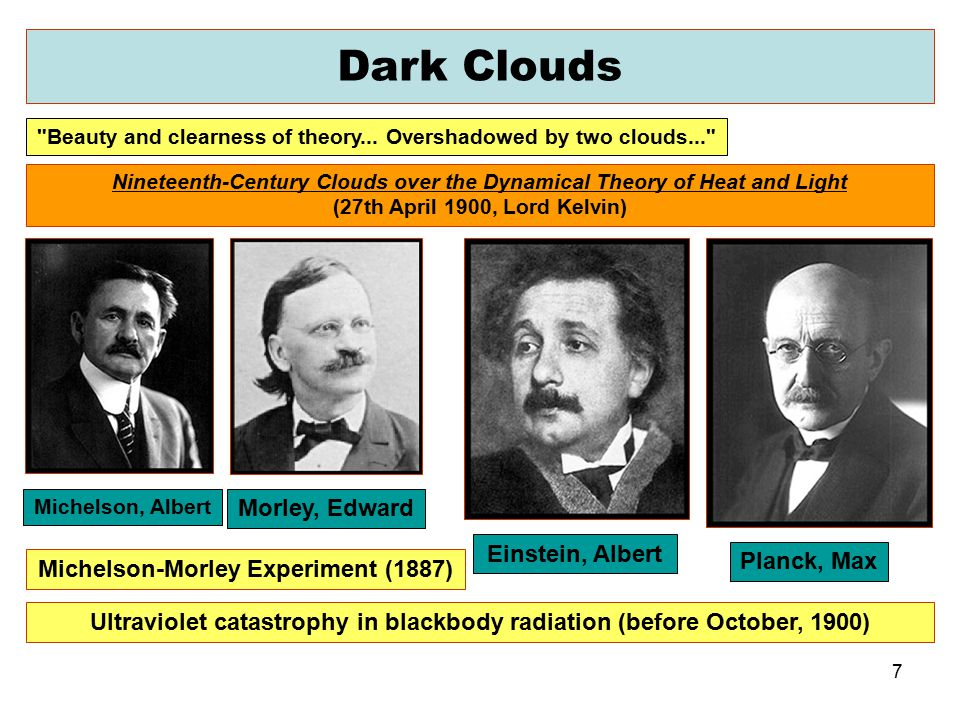
\includegraphics[height=2.40in,width=4.05in,viewport=0 50 735 470,clip]{Figures/Two-dark-cloud-in-physics-2.jpg}
%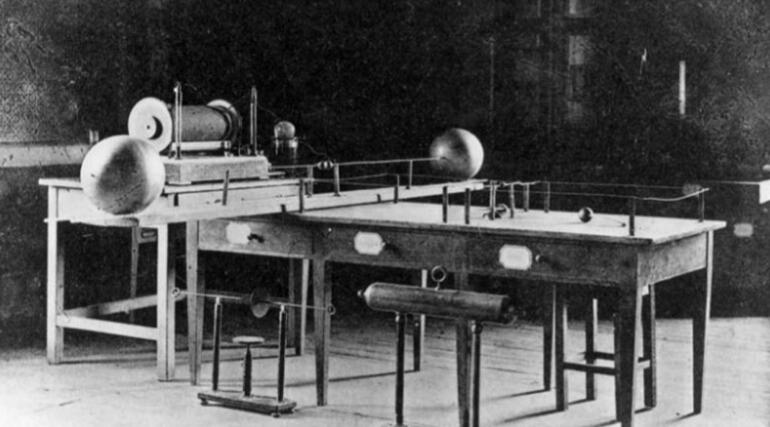
\includegraphics[height=2.40in,width=4.05in,viewport=0 0 580 325,clip]{Figures/Two-dark-cloud-in-physics-1.jpg}
\label{Classical_Mechanics}
\end{figure}
}

\frame
{
	\frametitle{\textrm{\small Newtonian, Lagrangian and Hamiltonian Mechanics}}
	\begin{itemize}
   		\setlength{\itemsep}{10pt}
		\item \textrm{\textcolor{blue}{Newtonian~Mechanics}}\\
		牛顿运动定律体系是以力、加速度、动量这些矢量为基本量来描述力学系统在欧氏空间的运动~(用几何方程表述约束)
	\item \textrm{\textcolor{blue}{Lagrangian~Mechanics}}\\
		拉格朗日力学是关于研究对象在其对应的约束系统下的运动形式,大大压缩牛顿方程描述需要的约束个数。不需要在另外设未知数目
	\item \textrm{\textcolor{blue}{Hamiltonian~Mechanics}}\\
		哈密度力学由拉格朗日力学演变而来,把位置和动量彻底分开,成为两种独立变量,由此诞生相空间。把广义动量和广义坐标放在等同的位置上(正则配对,方程降阶)
		\vskip 6pt
		拉格朗日力学和哈密顿力学的基本量是\textcolor{blue}{系统的能量}等标量,通过变分原理建立系统的动力学方程,所以拉格朗日力学和哈密顿力学合称\textcolor{magenta}{分析力学}
	\end{itemize}
}

\frame
{
	\frametitle{\textrm{Invariante Variationsprobleme}}
\begin{figure}[h!]
\centering
%
\vspace{-10.5pt}
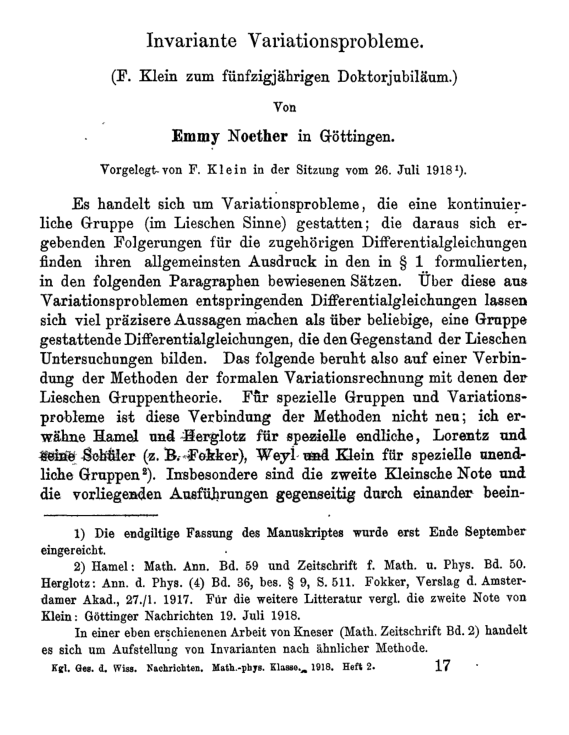
\includegraphics[height=0.52\textwidth,width=0.42\textwidth,viewport=0 0 450 580,clip]{Figures/Noether_theorem-1st_page.png}
\label{Noether_theorem}
\end{figure}
\begin{itemize}
\centering
	\item \textcolor{red}{能量守恒}~$\Longleftrightarrow$~\textcolor{magenta}{时间平移对称性}
	\item \textcolor{red}{动量守恒}~$\Longleftrightarrow$~\textcolor{magenta}{空间平移对称性}
	\item \textcolor{red}{角动量守恒}~$\Longleftrightarrow$~\textcolor{magenta}{空间旋转对称性}
\end{itemize}
}

\frame
{
	\frametitle{\textrm{驻波}}
\begin{figure}[h!]
\centering
\vspace{-15.5pt}
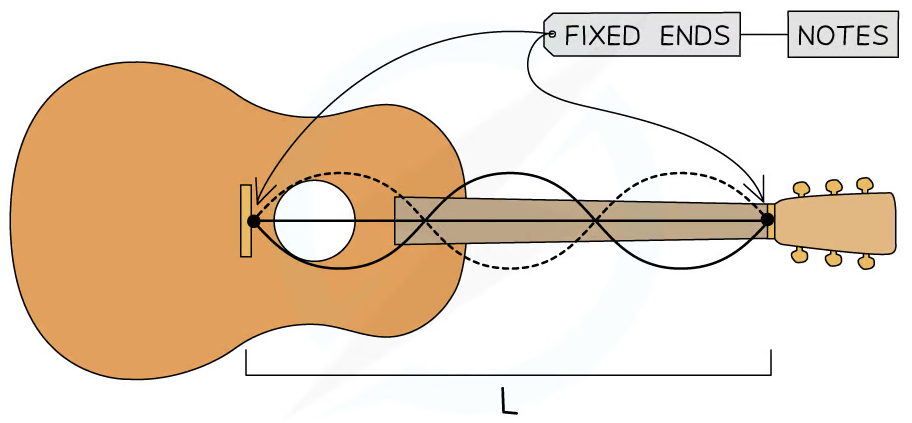
\includegraphics[height=0.40\textwidth,width=0.8\textwidth,viewport=0 0 900 450,clip]{Figures/Guitar-string.png}
\vskip 0.1pt
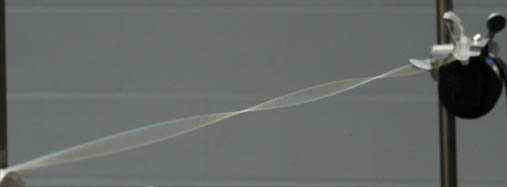
\includegraphics[height=0.35\textwidth,width=0.8\textwidth,viewport=0 0 122 48,clip]{Figures/string-standing-wave.jpg}
%\caption{\textrm{ABINIT}的Si.in}
\label{Standing_Wave_0}
\end{figure}
}

\frame
{
	\frametitle{驻波方程与势阱}
\begin{figure}[h!]
\centering
\vspace{-12.5pt}
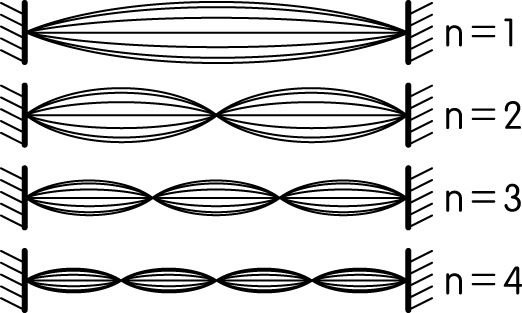
\includegraphics[height=0.32\textwidth,width=0.7\textwidth,viewport=0 0 125 75,clip]{Figures/Standing_wave.jpeg}
\vskip 2pt
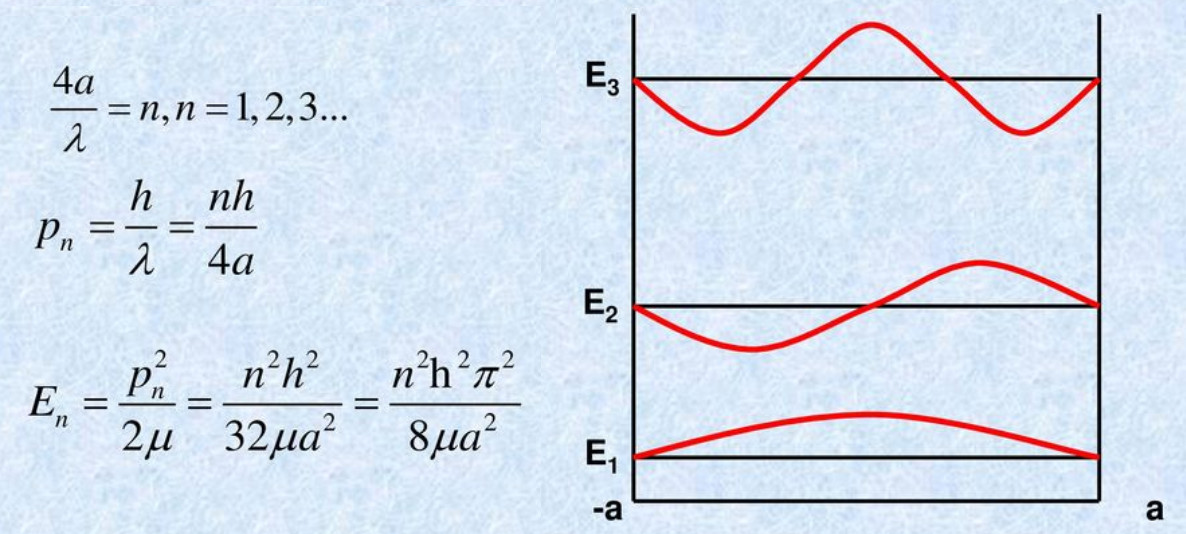
\includegraphics[height=0.40\textwidth,width=0.9\textwidth,viewport=0 0 1200 550,clip]{Figures/Standing_wave-energy.jpg}
%\caption{\textrm{ABINIT}的Si.in}
\label{Standing_Wave_1}
\end{figure}
}

\frame
{
	\frametitle{驻波方程与势阱}
\begin{figure}[h!]
\centering
\vspace{-5.5pt}
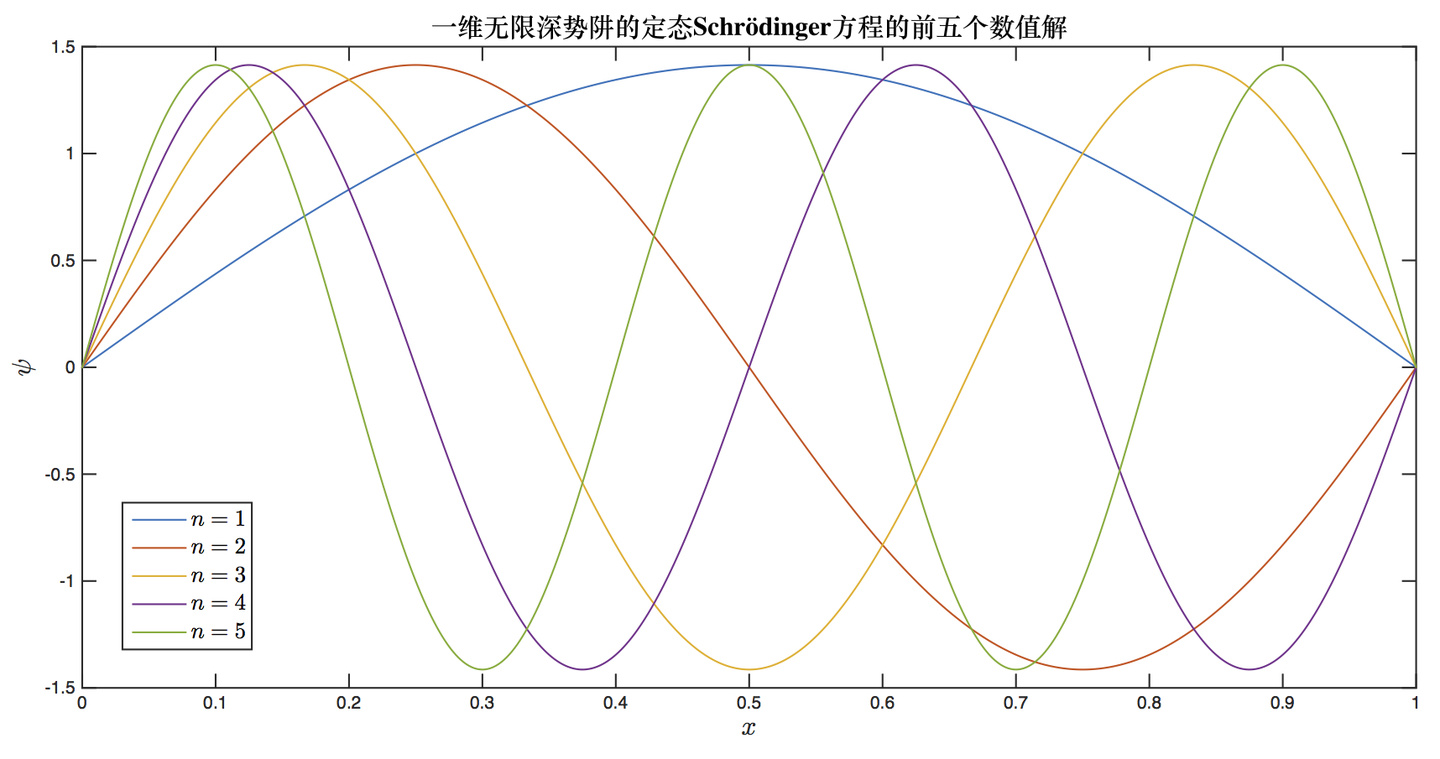
\includegraphics[height=0.55\textwidth,width=1.0\textwidth,viewport=0 0 720 400,clip]{Figures/Standing_wave-energy_1-5.jpg}
%\caption{\textrm{ABINIT}的Si.in}
\label{Standing_Wave_2}
\end{figure}
}

\frame
{
	\frametitle{驻波方程与势阱}
\begin{figure}[h!]
\centering
\vspace{-0.5pt}
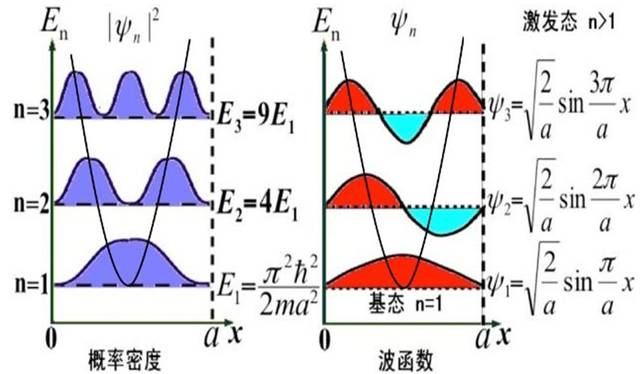
\includegraphics[height=0.46\textwidth,width=1.0\textwidth,viewport=0 0 650 390,clip]{Figures/Standing_wave_Energy.jpeg}
%\caption{\textrm{ABINIT}的Si.in}
\label{Standing_Wave_3}
\end{figure}
}

\frame
{
	\frametitle{原子中电子的驻波方程}
\begin{figure}[h!]
	\vspace{-10.5pt}
\centering
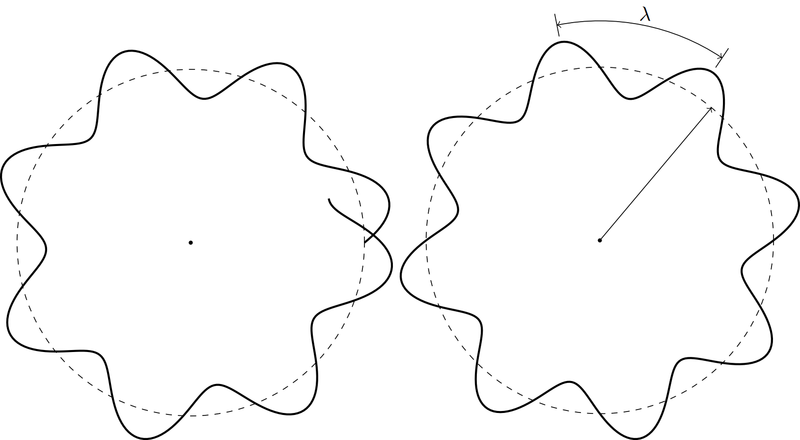
\includegraphics[height=0.38\textwidth,width=0.74\textwidth,viewport=0 0 840 440,clip]{Figures/Standing_wave-atom.png}
\vskip 2pt
\animategraphics[autoplay, loop, height=1.3in]{1}{Figures/Standing_wave_circle_}{1}{25}
\label{Atomic-electron_Standing_wave}
\end{figure}
}

\frame
{
	\frametitle{原子中的电子轨道和能量}
\begin{minipage}{0.43\textwidth}
\begin{figure}[h!]
%	\vspace{-14.8pt}
	\vspace{-4.8pt}
\centering
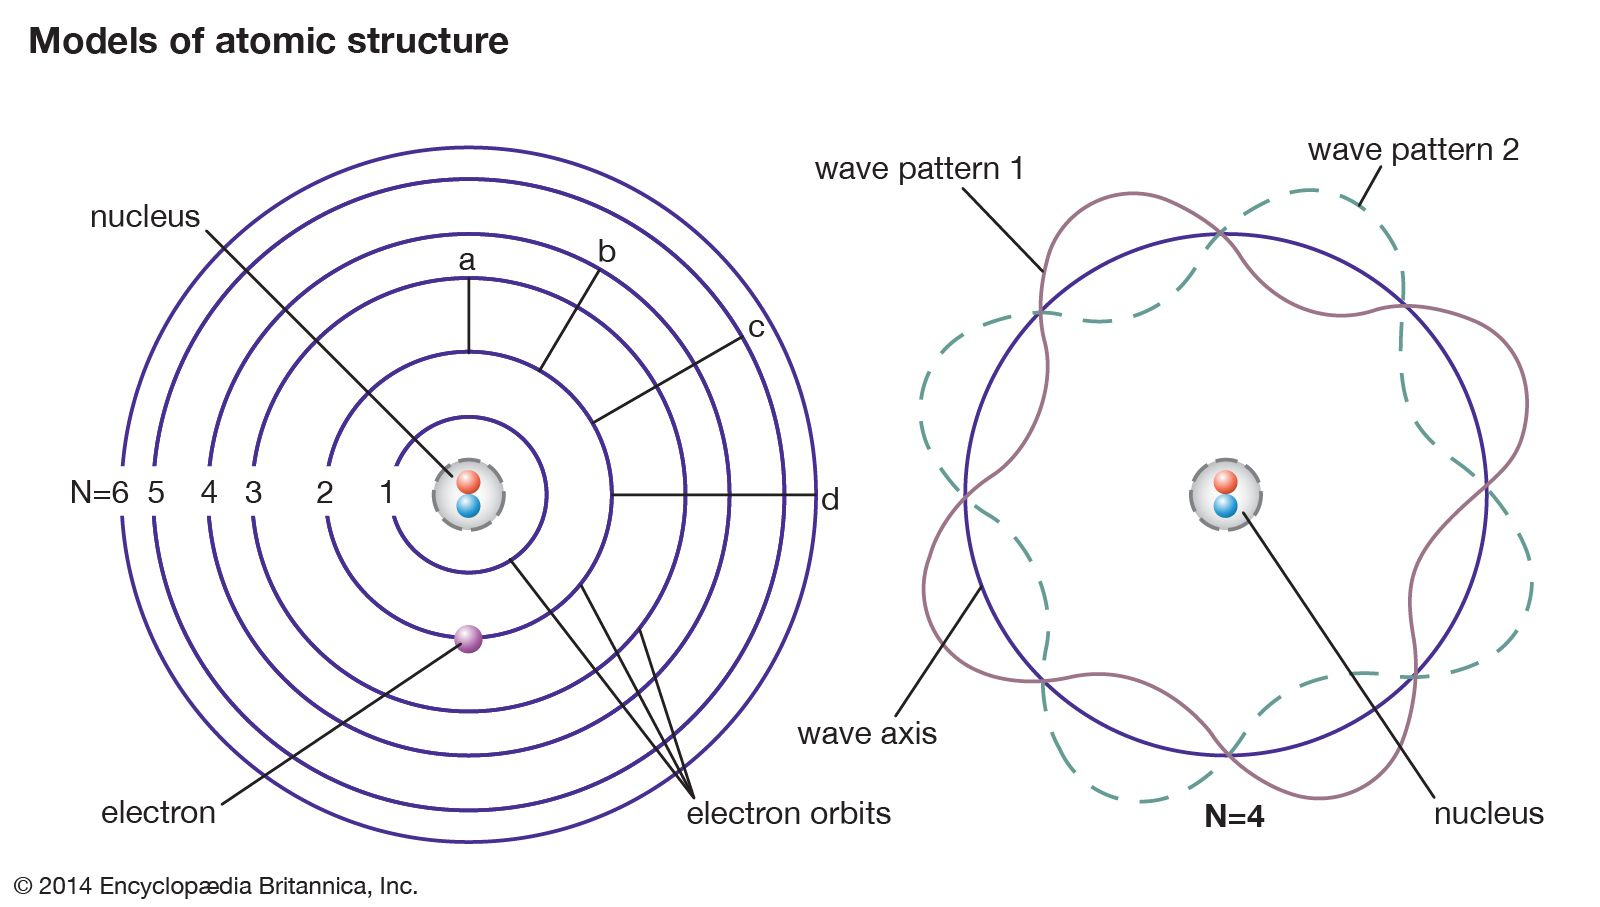
\includegraphics[height=0.57\textwidth,width=1.00\textwidth,viewport=0 50 1680 1000,clip]{Figures/electron-theory-Bohr-point-mass-energy-levels.jpg}
%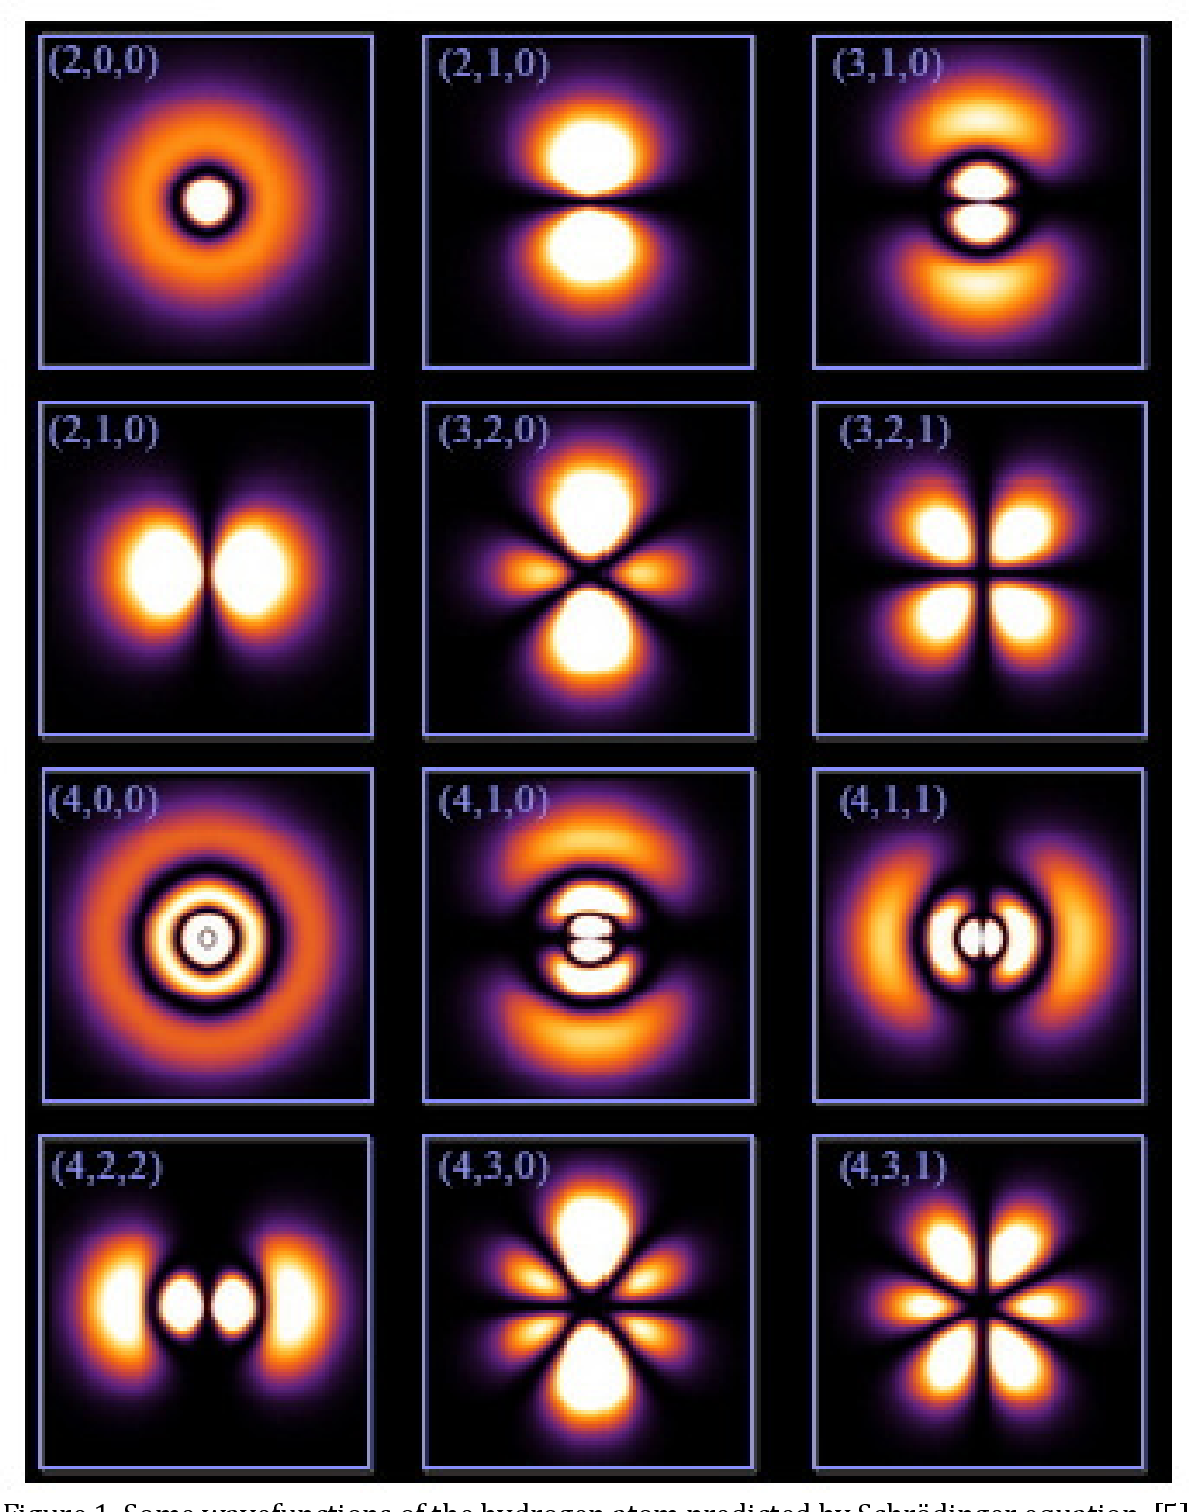
\includegraphics[height=1.23\textwidth,width=1.00\textwidth,viewport=0 10 1250 1500,clip]{Figures/wave_function.png}
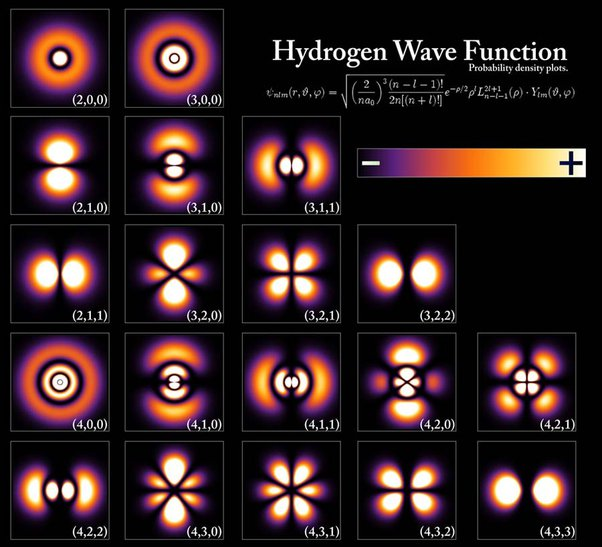
\includegraphics[height=0.95\textwidth,width=1.00\textwidth,viewport=0 0 630 650,clip]{Figures/wave_function-2.jpeg}
\label{Atomic-electron_wave}
\end{figure}
\end{minipage}
\begin{minipage}{0.55\textwidth}
\begin{figure}[h!]
	\vspace{-16.5pt}
\centering
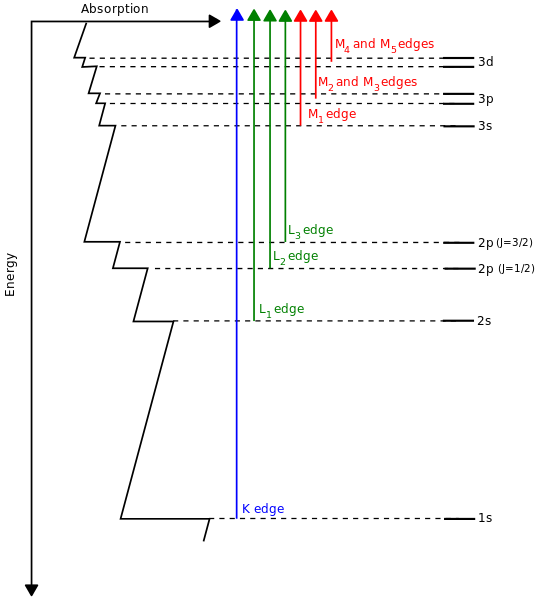
\includegraphics[height=1.10\textwidth,width=1.00\textwidth,viewport=0 0 560 600,clip]{Figures/Electron_orbital-energy.png}
\label{Atomic-electron_wave-energy}
\end{figure}
\end{minipage}
}

%\frame
%{
%	\frametitle{什么是“方程”}
%\begin{minipage}{0.45\textwidth}
%\begin{figure}[h!]
%	\vspace{-3.8pt}
%\centering
%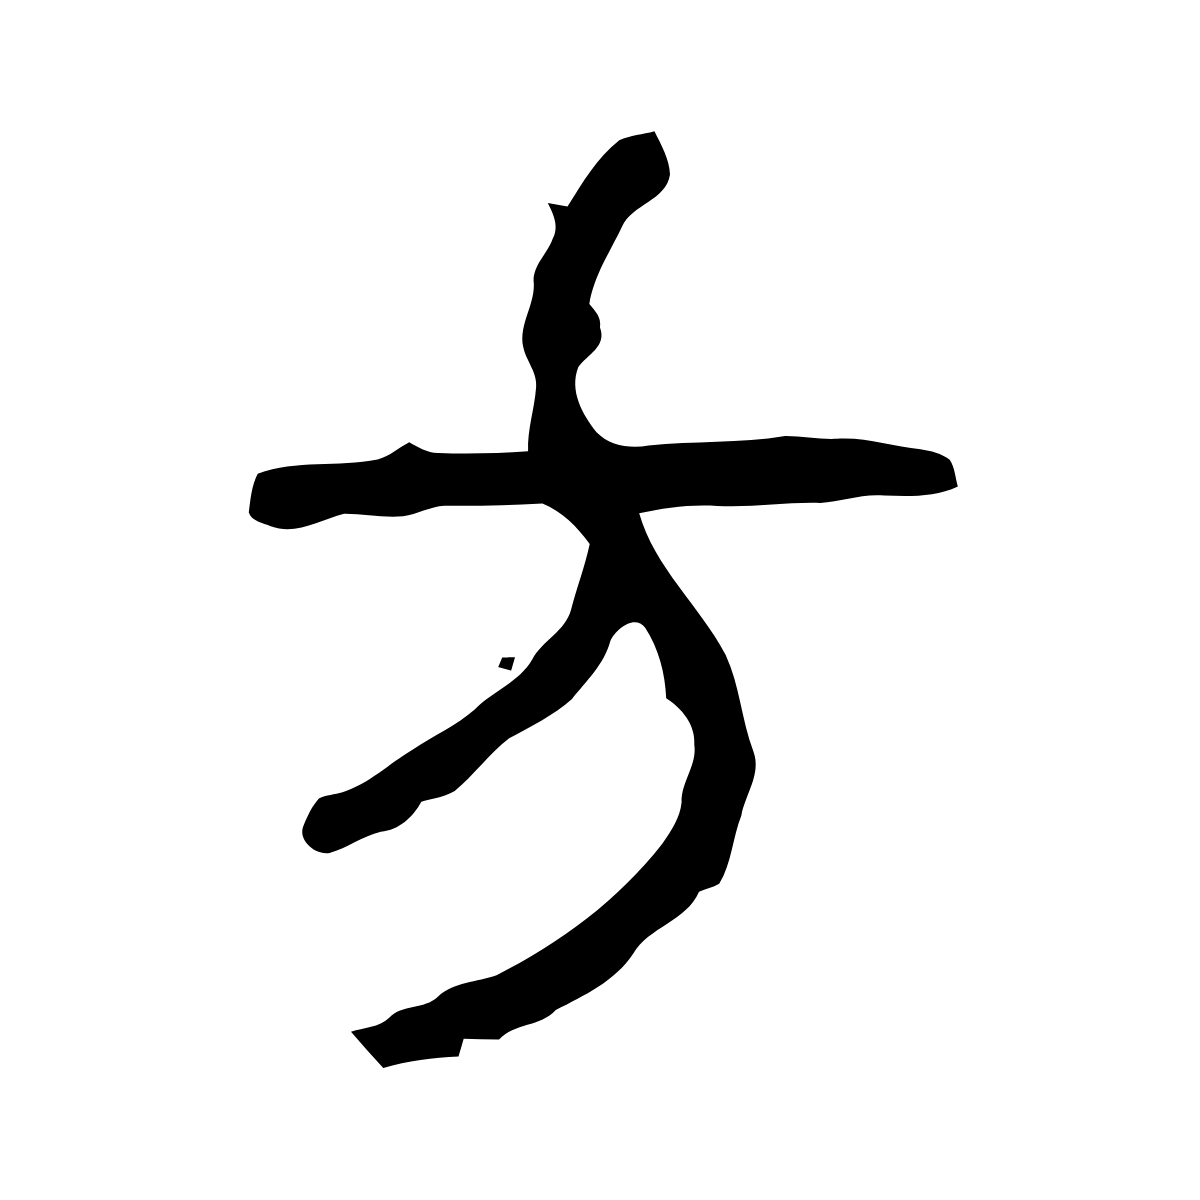
\includegraphics[height=0.60in,width=0.60in,viewport=0 0 1130 1130,clip]{Figures/Chinese_charater-equation-1.png}
%
\includegraphics[height=0.60in,width=0.60in,viewport=0 0 1130 1130,clip]{Figures/Chinese_charater-equation-2.png}
%\label{equation_1}
%\end{figure}
%\begin{figure}[h!]
%	\vspace{-15.8pt}
%\centering
%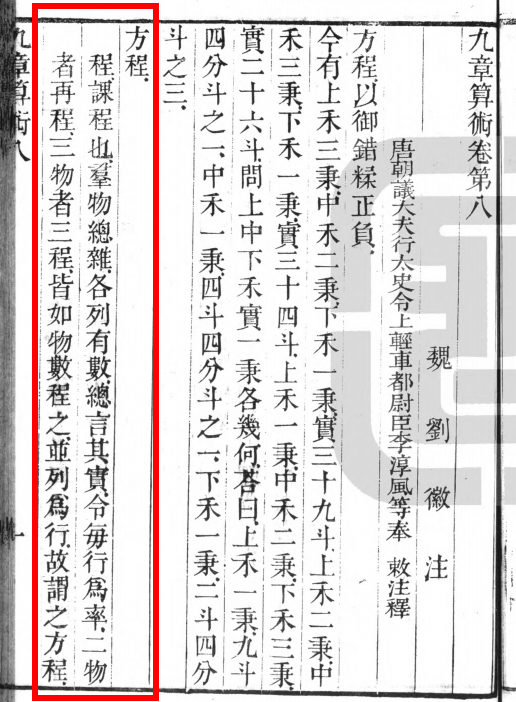
\includegraphics[height=2.20in,width=1.60in,viewport=0 0 520 700,clip]{Figures/Jiuzhang-8-equation_v1-1.png}
%\label{equation_2}
%\end{figure}
%\end{minipage}
%\begin{minipage}{0.53\textwidth}
%	{\fontsize{6.5pt}{5.2pt}\selectfont{
%	\vspace{-22.8pt}
%	\begin{itemize}
%		\item 方的本义是并,将两条船并起来,船头拴在一起,谓之方\\
%			\textcolor{purple}{\fontsize{5.5pt}{4.2pt}\selectfont{《说文》:~方,并船也。象两舟总头形。}}
%		\item 程的本义为称量谷物,并用作度量衡的总名\\
%			\textcolor{purple}{\fontsize{5.5pt}{4.2pt}\selectfont{《说文》:~程,品也。十髮爲程,十程爲分,十分爲寸。从禾呈聲。}}
%	\end{itemize}}}
%	\begin{itemize}
%		\item “\textcolor{blue}{课程}”{\fontsize{8.5pt}{6.2pt}\selectfont{指按不同物品的数量关系列出的计算式}}
%		\item “\textcolor{blue}{实}”{\fontsize{8.5pt}{6.2pt}\selectfont{指计算式中的常数项}}
%		\item “\textcolor{blue}{令每行为率}”,{\fontsize{8.5pt}{6.2pt}\selectfont{是由一个条件列一行计算式:~横列代表一个未知量}}
%		\item “\textcolor{blue}{如物数程之}”,{\fontsize{8.5pt}{6.2pt}\selectfont{就是有几个未知数就必须列出几个等式}}
%	\end{itemize}
%	\textcolor{red}{故而列出的一系列计算式称“方程”}
%\end{minipage}
%}
%
%\frame
%{
%	\frametitle{关于科学}
%\begin{figure}[h!]
%	\vspace{-3.8pt}
%\centering
%
\includegraphics[height=0.60in,width=0.60in,viewport=0 0 1130 1130,clip]{Figures/Chinese_charater-Science.png}
%
\includegraphics[height=0.60in,width=0.60in,viewport=0 0 1130 1130,clip]{Figures/Chinese_charater-equation-2.png}
%\label{Science_1}
%\end{figure}
%	\begin{itemize}
%		\item 科的本义是品类,等级\\
%			\textcolor{purple}{\fontsize{5.5pt}{4.2pt}\selectfont{《说文》:~科,程也。从禾从斗。斗者,量也。}}
%		\item 程的本义为称量谷物,并用作度量衡的总名\\
%			\textcolor{purple}{\fontsize{5.5pt}{4.2pt}\selectfont{《说文》:~程,品也。十髮爲程,十程爲分,十分爲寸。从禾呈聲。}}
%	\end{itemize}
%	\begin{itemize}
%		\item “科学”一词由近代日本学界率先使用,初用于对译英文中的\textcolor{red}{\textrm{Science}}及其它欧洲语言中的相应词汇,欧洲语言中该词来源于拉丁文\textcolor{red}{\textrm{Scientia}},\textcolor{blue}{意为“知识”与“学问”},在近代侧重关于自然的学问。在日本幕府末期到明治时期,“科学”是专门的“个别学问”,有的在以“分科的学问”的意义被使用
%	\end{itemize}
%	“\textcolor{blue}{科学}”一词经日本传入中国,命名其取\textcolor{purple}{分类、测量之学问}之义
%}
%
\frame
{
	\frametitle{\textrm{Schr\"odinger}~方程}
\begin{minipage}{0.49\textwidth}
\begin{figure}[h!]
\centering
%
\vspace{-25.5pt}
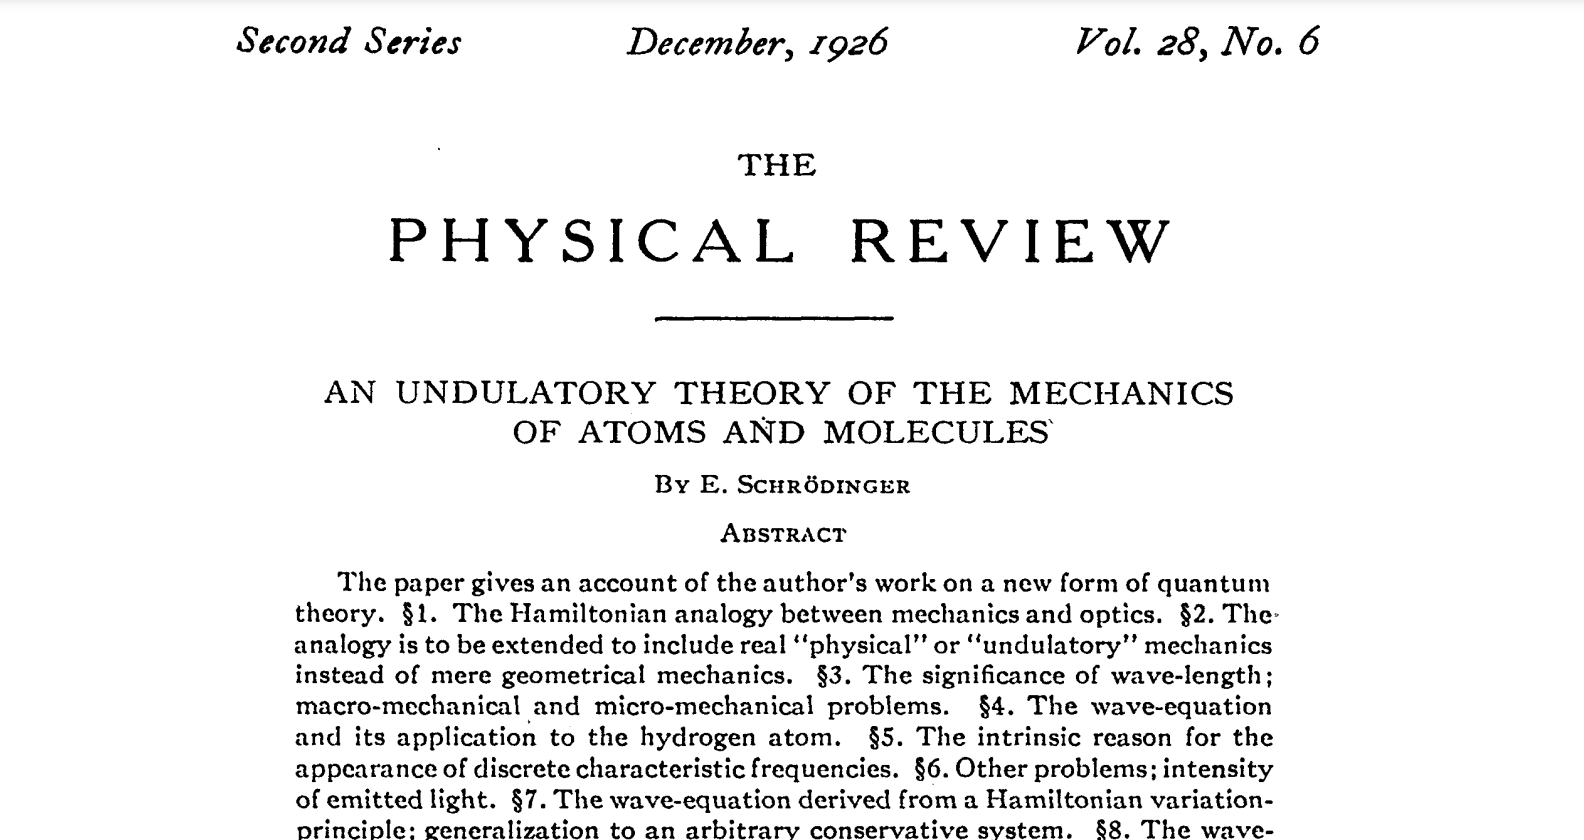
\includegraphics[height=1.80in,width=2.00in,viewport=180 0 1380 1100,clip]{Figures/Schrodinger_article.png}
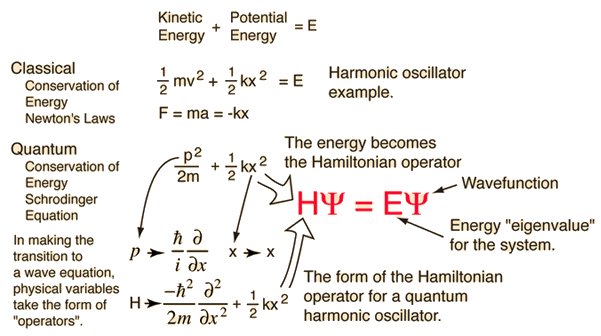
\includegraphics[height=1.20in,width=2.00in,viewport=0 0 600 350,clip]{Figures/Schrodinger_Equation.png}
\label{Schrodinger_Equation}
\end{figure}
\end{minipage}
\begin{minipage}{0.49\textwidth}
\begin{figure}[h!]
\centering
%
\vspace{-15.5pt}
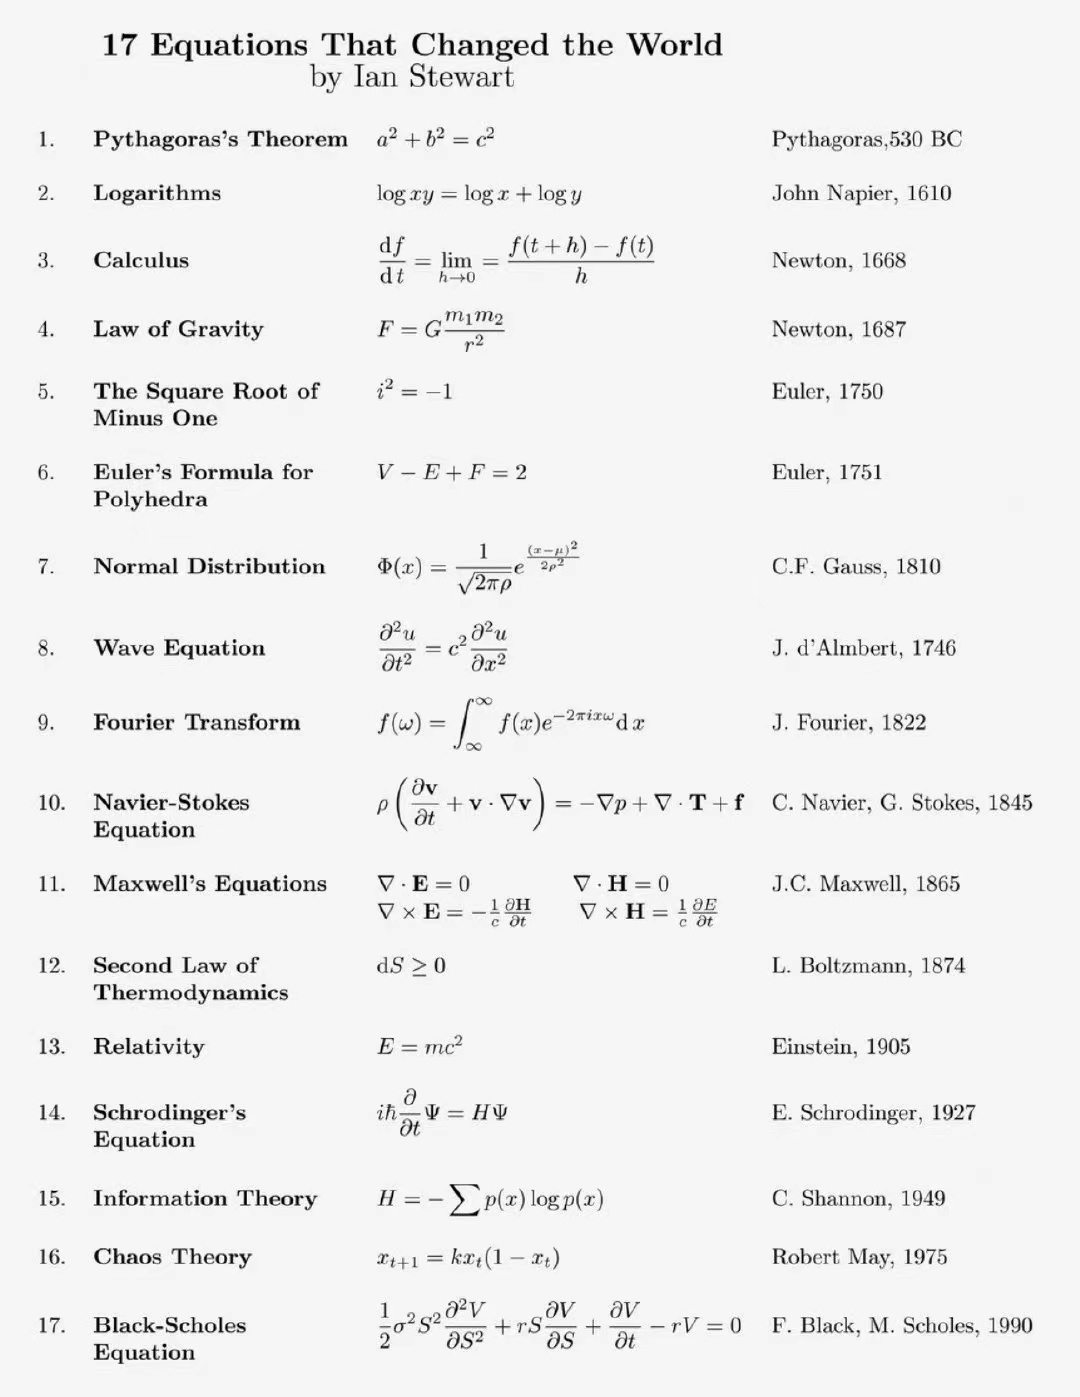
\includegraphics[height=2.85in,width=2.00in,viewport=0 0 780 1100,clip]{Figures/Great_Equation.jpg}
\label{Great_Equation}
\end{figure}
\end{minipage}
}

\frame
{
	\frametitle{量子力学的奠基人}
\begin{figure}[h!]
\centering
%\vspace{-25.5pt}
%\hspace*{-15.5pt}
%\includegraphics[height=0.57\textwidth,width=1.1\textwidth,viewport=0 0 2150 1050,clip]{Figures/Solvay_Conference-5-fine.jpg}
\vspace{-14.5pt}
\hspace*{-15.5pt}
\includegraphics[height=0.50\textwidth,width=0.70\textwidth,viewport=150 105 850 710,clip]{Figures/Solvay_Conference-5.jpg}
\caption{\fontsize{7.5pt}{6.2pt}\selectfont{\textrm{The Fifth Solvay International Conference, Brussels, Belgium, Oct. 1927}}}
\label{Solvay Conference-5-fine}
\end{figure}
\vspace{-11.5pt}
\fontsize{4.1pt}{3.9pt}\selectfont{\textrm{\textcolor{blue}{前排左起}:~I.Langmuir(\textcolor{blue}{朗缪尔}) M.Planck(\textcolor{blue}{普朗克}) Marie Curie(\textcolor{blue}{居里夫人}) H.Lorentz(\textcolor{blue}{洛仑兹}) A.Einstein(\textcolor{blue}{爱因斯坦}) P.Langevin(\textcolor{blue}{朗之万}) Ch.E.Guye(\textcolor{blue}{古伊}) C.T.R.Wilson(\textcolor{blue}{威尔逊}) O.W.Richardson(\textcolor{blue}{理查森})\\
\textcolor{blue}{中排左起}:~P.Debye(\textcolor{blue}{德拜}) M.Knudsen(\textcolor{blue}{克努森}) W.L.Bragg(\textcolor{blue}{布拉格}) H.A.Kramers(\textcolor{blue}{克莱默}) P.A.M.Dirac(\textcolor{blue}{狄拉克}) A.H.Compton(\textcolor{blue}{康普顿}) L.de Broglie(\textcolor{blue}{德布罗意}) M.Born(\textcolor{blue}{玻恩}) N.Bohr(\textcolor{blue}{玻尔})\\
\textcolor{blue}{后排左起}:~A.Piccard(\textcolor{blue}{皮卡尔德}) E.Henriot(\textcolor{blue}{亨利厄特}) P.Ehrenfest(\textcolor{blue}{埃伦费斯特}) Ed.Herzen(\textcolor{blue}{赫尔岑}) Th.de Donder(\textcolor{blue}{德唐德}) E.Schr\"odinger(\textcolor{blue}{薛定谔}) E.Verschaffelt(\textcolor{blue}{费尔夏费尔特}) W.Pauli(\textcolor{blue}{泡利}) W.Heisenberg(\textcolor{blue}{海森堡}) R.H.Fowler(\textcolor{blue}{富勒}) L.Brillouin(\textcolor{blue}{布里渊})}}
}

\frame
{
	\frametitle{态叠加原理:~\textrm{Schr\"odinger's cat}}
\begin{figure}[h!]
\centering
\vspace{-10.5pt}
\includegraphics[height=0.70\textwidth,width=0.48\textwidth,viewport=0 0 550 750,clip]{Figures/Schrodinger-cat.jpg}
\includegraphics[height=0.70\textwidth,width=0.50\textwidth,viewport=0 0 720 930,clip]{Figures/Schrodinger_book.jpg}
%\caption{\textrm{ABINIT}的Si.in}
\label{Schrodinger-cat}
\end{figure}
}

\frame
{
	\frametitle{因果倒置:~\textrm{Delayed Choice Experiment}}
\begin{figure}[h!]
\centering
\vspace{-10.5pt}
\includegraphics[height=0.55\textwidth,width=1.0\textwidth,viewport=0 0 690 370,clip]{Figures/Schematic-diagram-of-delayed_choice-experiment.png}
\caption{\fontsize{5.2pt}{3.9pt}\selectfont{\textrm{Schematic diagram of Wheeler's delayed choice experiment with A Mach-Zehnder Interferometer.}}}
\label{Delayed_Choice-Experiment}
\end{figure}
}

\frame
{
	\frametitle{量子力学量力学}
\begin{figure}[h!]
\centering
\vspace{-13.5pt}
\includegraphics[height=0.75\textwidth,width=0.55\textwidth,viewport=0 0 500 650,clip]{Figures/Quote-Niels_Bohr-on-Quantum_mechanics.png}
\caption{\fontsize{5.2pt}{3.9pt}\selectfont{\textrm{A quote of Niels Bohr on Quantum mechanics.}}}
\label{Quote-Niels_Bohr}
\end{figure}
}

\frame
{
	\frametitle{量子力学的解释}
\begin{figure}[h!]
\centering
\vspace{-12.5pt}
\includegraphics[height=0.745\textwidth,width=0.65\textwidth,viewport=300 150 1800 1870,clip]{Figures/Interpretation-QM.png}
\caption{\fontsize{5.2pt}{3.9pt}\selectfont{\textrm{Interpretation of Quantum mechanics.}}}
\label{Interpretation-QM}
\end{figure}
}

\frame
{
	\frametitle{几何原本:~公理体系的源头}
\begin{figure}[h!]
\centering
\vspace{-13pt}
\includegraphics[height=0.38\textwidth,width=0.65\textwidth,viewport=0 0 680 500,clip]{Figures/Element_Geometry_1.jpg}\\
\vspace{1pt}
\includegraphics[height=0.36\textwidth,width=0.65\textwidth,viewport=0 0 810 500,clip]{Figures/Element_Geometry_2.jpg}
%\caption{\textrm{ABINIT}的Si.in}
\label{Element_Geometru}
\end{figure}
}

%\begin{frame}
%	\frametitle{数的信仰}
%\begin{figure}[h!]
%\centering
%\vspace{-15.5pt}
%\includegraphics[height=1.30in,width=2.60in,viewport=0 0 600 290,clip]{Figures/pythagorean_numerology.png}
%\includegraphics[height=1.20in,width=2.60in,viewport=0 0 850 400,clip]{Figures/quote_pythagoras.jpg}
%\caption{\tiny 万物皆数\textrm{(All is number)}信仰}
%\label{Pythagoras_numerology}
%\end{figure}
%\end{frame}
%
%\begin{frame}
%	\frametitle{无理数的挑战}
%	\begin{itemize}
%		\item \textcolor{red}{有理数}:~\textrm{rational number} ~~~ {\fontsize{7.5pt}{6.0pt}\selectfont{\textcolor{magenta}{\textrm{rate}} $\Longrightarrow$ \textrm{ration} $\longrightarrow$ \textcolor{violet}{\textrm{rational}}}}
%		\item \textcolor{blue}{无理数}:~\textrm{irrational number}
%	\end{itemize}
%\begin{figure}[h!]
%\centering
%\vspace{-10.5pt}
%\includegraphics[height=1.80in,width=1.80in,viewport=0 0 110 110,clip]{Figures/Pi_sqrt2.jpeg}
%\includegraphics[height=1.80in,width=1.80in,viewport=0 0 317 316,clip]{Figures/coordinate-plane.png}
%\caption{\tiny \textrm{$\pi$、$\sqrt 2$、$\sqrt 3$ from a circle and a coordinate plane.}}
%\label{Pi_sqrt2}
%\end{figure}
%\end{frame}
%
%\begin{frame}
%	\frametitle{复数的物理意义}
%	\begin{displaymath}
%		\textcolor{blue}{z}=a+b\textcolor{red}{\mathbf{i}}
%	\end{displaymath}
%\begin{figure}[h!]
%\centering
%\vspace{-5.5pt}
%\includegraphics[height=1.90in,width=4.00in,viewport=0 0 1052 566,clip]{Figures/RLC_series_circuit.png}
%\caption{\tiny \textrm{The imaginary in RLC series circuit.}}
%\label{complex_imaginary}
%\end{figure}
%\end{frame}
%
\frame
{
	\frametitle{\textcolor{red}{公理体系}:~现代科学的逻辑起点}
\begin{figure}[h!]
\centering
\vspace{-10.5pt}
\includegraphics[height=0.68\textwidth,width=1.0\textwidth,viewport=0 0 770 500,clip]{Figures/Philp_Nature_Mach-2.png}
%\caption{\textrm{ABINIT}的Si.in}
\label{Philp_Nature}
\end{figure}
}

\frame[allowframebreaks]
{
	\frametitle{量子力学基本假设(\textcolor{red}{公理体系})}
	\begin{itemize}
		\item 全同粒子假设\\
			\textcolor{blue}{全同粒子组成的体系中,两个全同粒子相互调换不改变体系的状态}\\ 
			全同粒子是指\textcolor{red}{内禀性质完全相同的一类微观粒子}:\\例如,所有的电子是全同粒子 
		\item 波函数假设\\
			\textcolor{blue}{微观体系的运动状态可由波函数$\Psi$完全描述,波函数包含体系的所有性质}\\
			波函数$\Psi$一般要求满足\textcolor{red}{连续}、\textcolor{red}{有限}和\textcolor{red}{单值}三个条件
		\item 微观体系的运动状态\textcolor{blue}{波函数随时间变化的规律}:\\\textcolor{red}{遵从\textrm{Schr\"odinger}方程}
			$$\mathrm{i}\hbar\dfrac{\mathrm{d}}{\mathrm{d}t}|\Psi\rangle=\hat{\mathbf H}|\Psi\rangle$$
		\item 态叠加原理\\
			如果$\Psi_1$是体系的一个本征态,对应的本征值为$A_1$,$\Psi_2$也是体系的一个本征态,对应的本征值为$A_2$,则\textcolor{blue}{$$\Psi=C_1\Psi_1+C_2\Psi_2$$}\textcolor{red}{也是体系一个可能的存在状态}
		\item 力学量算符假设\\
			\textcolor{blue}{经典力学的物理量对应到量子力学中,要用线性~\textrm{Hermite}算符表示}(\textcolor{red}{\textrm{Hermite~}算符的本征函数构成完备空间})\\
			如动量算符 ~~~ $\hat{\mathbf{p}}=-\mathrm{i}\hbar\nabla$\\
			~~~位置算符 ~~~ $\hat{\mathbf r}=r$\\
			力学量算符之间有确定的对易关系(\textcolor{brown}{量子条件})
			$$[\hat{\mathbf F},\hat{\mathbf G}]=\hat{\mathbf F}\hat{\mathbf G}-\hat{\mathbf G}\hat{\mathbf F}$$ 
			
	\end{itemize}
}

\frame
{
	\frametitle{叠加态的数学表示:~矩阵}
\begin{figure}[h!]
\centering
\vspace{-1.5pt}
\hspace*{-0.12in}
\includegraphics[height=0.48\textwidth,width=1.05\textwidth]{Figures/Matrix_Rotation.png}
%\caption{\textrm{ABINIT}的Si.in}
\label{Matrix-Rotation}
\end{figure}
}

\frame
{
	\frametitle{量子化学学科创立}
	\begin{itemize}
		\item \textrm{1927}年,\textrm{\o.~Burrau}应用量子力学原理,完成\textrm{\ch{H2+}}离子的计算
		\item 同年,\textrm{Walter~Heitlery}和\textrm{Fritz~W.~London}对\textrm{\ch{H2}}分子的计算,标志着量子化学这一学科正式创立
	\end{itemize}
\begin{figure}[h!]
\centering
\vspace{-1.5pt}
\hspace*{-0.12in}
\includegraphics[height=0.48\textwidth,width=0.80\textwidth,viewport=0 10 260 175,clip]{Figures/Walter-Heitlery_Fritz-W-London.jpeg}
\caption{\textrm{W.~Heitlery (left) and F.~W.~London(right).}}
\label{Heitlery_London}
\end{figure}
}

\section{量子力学与化学键的本质}
\subsection{分子轨道理论}
\frame
{
	\frametitle{原子核外电子排布}
\begin{figure}[h!]
\vspace*{-0.35in}
\centering
\includegraphics[height=1.35in,width=2.95in,viewport=0 0 500 230,clip]{Figures/Li-Na-K.png}
\includegraphics[height=1.92in,width=3.65in,viewport=0 0 500 275,clip]{Figures/Ne-Ar-Kr.png}
%\caption{\tiny \textrm{Pseudopotential for metallic sodium, based on the empty core model and screened by the Thomas-Fermi dielectric function.}}%(与文献\cite{EPJB33-47_2003}图1对比)
\label{Electron_in_atom}
\end{figure}
}

\frame
{
	\frametitle{$\mathrm{O}_2$分子轨道}
\begin{figure}[h!]
\centering
\vspace{-15.5pt}
\includegraphics[height=0.60in,width=3.35in,viewport=0 100 500 200,clip]{Figures/Octet-Rule-O2_CO2.png}
\includegraphics[height=2.25in,width=1.90in,viewport=0 0 150 170,clip]{Figures/MO-O2.png}
%\caption{\textrm{The wave-particle duality and Photoelectric effect}}
\label{MO:O2}
\end{figure}
}

\frame
{
	\frametitle{$\mathrm{N}_2$分子轨道}
\begin{figure}[h!]
\centering
\vspace{-10.5pt}
\includegraphics[height=0.60in,width=2.55in,viewport=0 0 500 130,clip]{Figures/Octet-Rule-N2.png}
\includegraphics[height=2.30in,width=2.15in,viewport=0 0 160 150,clip]{Figures/MO-N2.png}
%\caption{\textrm{The wave-particle duality and Photoelectric effect}}
\label{MO:N2}
\end{figure}
}

\frame
{
	\frametitle{共价化合物的分子轨道}
\begin{figure}[h!]
\centering
\vspace{-5.5pt}
\includegraphics[height=2.30in,width=1.75in,viewport=0 0 400 460,clip]{Figures/Molecular-orbital-diagram-of-HF.png}
\includegraphics[height=2.65in,width=2.05in,viewport=0 0 560 750,clip]{Figures/Molecular-orbital-diagram-of-CO.png}
%\caption{\textrm{The wave-particle duality and Photoelectric effect}}
\label{MO:HF}
\end{figure}
}

\subsection{分子的稳定性与键级}
\frame
{
	\frametitle{分子轨道与键强度}
\begin{figure}[h!]
\centering
\vspace{-10.5pt}
%\caption{\textrm{The wave-particle duality and Photoelectric effect}}
\includegraphics[height=1.30in,width=4.00in,viewport=0 0 325 110,clip]{Figures/MO-diagrams_H2He2.png}
\includegraphics[height=1.20in,width=4.00in,viewport=0 0 360 100,clip]{Figures/multi-orbital.png}
\label{MO:H2-He}
\end{figure}
}

\frame
{
	\frametitle{键级的估算}
\begin{figure}[h!]
\centering
\vspace{-10.5pt}
%\caption{\textrm{The wave-particle duality and Photoelectric effect}}
\includegraphics[height=3.00in,width=4.00in,viewport=0 0 1500 1050,clip]{Figures/Band-order.png}
\label{Bond_Order}
\end{figure}
}

\frame
{
	\frametitle{键级的估算}
\begin{figure}[h!]
\centering
\vspace{-15.5pt}
%\caption{\textrm{The wave-particle duality and Photoelectric effect}}
\includegraphics[height=2.80in,width=4.10in,viewport=0 0 800 550,clip]{Figures/Band-order-2.jpg}
\label{Bond_Order-2}
\end{figure}
}

%\subsection{化学键的本质}
\frame
{
	\frametitle{轨道杂化与分子结构}
\begin{figure}[h!]
\centering
\vspace{-10.5pt}
%\caption{\textrm{The wave-particle duality and Photoelectric effect}}
\includegraphics[height=2.75in,width=4.00in,viewport=0 0 520 370,clip]{Figures/methane-gas.png}
\label{Bond_Hybrid}
\end{figure}
}

\frame
{
	\frametitle{化学键的本质}
\begin{figure}[h!]
\centering
\vspace{-10.5pt}
%\caption{\textrm{The wave-particle duality and Photoelectric effect}}
\includegraphics[height=2.80in,width=2.00in,viewport=0 0 1600 2050,clip]{Figures/Linus_Pauling.jpeg}
\includegraphics[height=2.80in,width=1.85in,viewport=0 0 420 650,clip]{Figures/The-Nature-of-the-Chemical-Bond_content.png}
\label{Pauling:Bond_Hybrid}
\end{figure}
}

\frame
{
	\frametitle{分子轨道与价键}
\begin{figure}[h!]
\centering
\vspace{-10.5pt}
%\caption{\textrm{The wave-particle duality and Photoelectric effect}}
\includegraphics[height=1.50in,width=1.70in,viewport=0 0 820 680,clip]{Figures/MO-CH4.jpg}
\includegraphics[height=1.45in,width=4.00in,viewport=0 0 2100 750,clip]{Figures/methane-sp3.png}
\label{MO-vs-VB:CH4}
\end{figure}
}

\frame
{
	\frametitle{分子轨道与价键}
\begin{figure}[h!]
\centering
\vspace{-10.5pt}
%\caption{\textrm{The wave-particle duality and Photoelectric effect}}
\includegraphics[height=2.40in,width=4.00in,viewport=0 0 1050 630,clip]{Figures/QM_bond-order.jpg}
\label{MO-vs-VB}
\end{figure}
{\centering 分子轨道理论\textrm{~.vs.~}价键理论:~\textcolor{red}{横看成岭侧成峰}}
}

\frame
{
	\frametitle{复杂分子的前线轨道:\textrm{HOMO}}
\begin{figure}[h!]
\centering
\vspace{-10.5pt}
%\caption{\textrm{The wave-particle duality and Photoelectric effect}}
\includegraphics[height=2.20in,width=3.80in,viewport=0 0 900 570,clip]{Figures/Molecular-orbital-diagram-of-the-most-important-occupied-occupied-orbital-overlap_2.png}
\label{HOMO-LUMO:HOMO}
\end{figure}
\textrm{\textcolor{blue}{HOMO}:~the Highest Occupied Molecular Orbital}
}

\frame
{
	\frametitle{复杂分子的前线轨道:\textrm{HOMO-LUMO}}
\begin{figure}[h!]
\centering
\vspace{-10.5pt}
%\caption{\textrm{The wave-particle duality and Photoelectric effect}}
\includegraphics[height=2.50in,width=2.00in,viewport=0 40 750 850,clip]{Figures/HOMO-LUMO.jpg}
\label{HOMO-LUMO:LUMO}
\end{figure}
\textrm{\textcolor{blue}{LUMO}:~the Lowest Unoccupied Molecular Orbital}
}

\frame
{
	\frametitle{前线轨道与化学反应}
\begin{figure}[h!]
\centering
\vspace{-10.5pt}
%\caption{\textrm{The wave-particle duality and Photoelectric effect}}
\includegraphics[height=2.80in,width=3.90in,viewport=0 0 550 400,clip]{Figures/NH3_BCl3_HOMO_LUMO_orient.jpg}
\label{HOMO-LUMO}
\end{figure}
}

%\frame
%{
%	\frametitle{\textrm{Paul Adrian Maurice Dirac's Commandments}}
%	\textrm{The underlying laws necessary for the mathematical treatment of a large part of physics \textcolor{red}{and the whole of chemistry} are thus completely known, and the difficulty lies only in the fact that application of these laws leads to equations that are \underline{too complex to be solved}.
%\vskip 15pt
%It therefore becomes desirable that approximation practical methods of applying quantum mechanics should be develop $\cdots$ 
%}

%\vskip 15pt
%\textrm{P.A.M Dirac Proc. Roy. Soc. Ser. A, \textbf{123}, 714, (1929)}
%}
%
\frame
{
%	\frametitle{\rm{Paul Dirac's Commandments\upcite{PRSLSA123-714_1929}}}
	\frametitle{\textrm{Paul Dirac's Commandments}}%\upcite{PRSLSA123-714_1929}}}
%	\textrm{\textcolor{purple}{The underlying laws necessary for the mathematical treatment of a large part of physics and the whole of chemistry are thus completely known, and the difficulty lies only in the fact that application of these laws leads to equations that are too complex to be solved.}}
\begin{figure}[h!]
\centering
\vspace{-10.5pt}
\includegraphics[height=0.71\textwidth,width=0.9\textwidth,viewport=0 0 1150 920,clip]{Figures/Dirac_comment.png}
%\caption{\textrm{ABINIT}的Si.in}
\label{Diract_Commandment}
\end{figure}
}

\frame
{
%	\frametitle{\textrm{DFT-SCF}}
\begin{figure}[h!]
\vspace*{-0.25in}
\centering
\includegraphics[height=2.80in,width=4.95in,viewport=5 3 1250 780,clip]{Figures/Method_Procedure.png}
%\caption{\tiny \textrm{Pseudopotential for metallic sodium, based on the empty core model and screened by the Thomas-Fermi dielectric function.}}%(与文献\cite{EPJB33-47_2003}图1对比)
\label{Method-Procedure-copy}
\end{figure}
}

\frame
{
	\frametitle{王守竞先生与量子力学}
	王守竞(\textrm{Shou~Chin~Wang})的工作
	\begin{itemize}
		\item 计算氢分子的电子结构
			\vskip 2.5pt
			王守竞的论文\textcolor{purple}{《新量子力学下的常态氢分子问题》}%THE PROBLEM OF THE NORMAL HYDROGEN MOLECULE IN THE NEW QUANTUM MECHANICS
	\textcolor{blue}{
	\begin{displaymath}
		\Psi=C\left\{ \mathrm{exp}[-Z(r_1+ p_2)/a]+\mathrm{exp}[-Z( r_2+ p_1)/a] \right\}
	\end{displaymath}}
	{\fontsize{7.2pt}{6.5pt}\selectfont{其中$r_1$、$p_1$是第一个电子到两个原子核的距离,$r_2$,$p_2$是第二个电子到两个原子核的距离,$a$是\textrm{Bohr}半径}}\\
	得到的数值结果$Z=1.666$,$E_0=86.6\,\mathrm{kcal}$,$R_0=0.78$\,\textrm{\AA}
		\item 不对称陀螺(不对称转动)的能谱%On the Asymmetrical Top in Quantum Mechanics
			\vskip 2.5pt
			不对称陀螺的能级公式(\textcolor{purple}{“王氏公式”})
	\textcolor{blue}{
	\begin{displaymath}
		E= (hc8\pi)[Aj(j+1)+W]
	\end{displaymath}}
	\end{itemize}
}

\frame
{
	\frametitle{王守竞先生与量子力学}
\begin{figure}[h!]
\centering
\vspace{-10.5pt}
\includegraphics[height=0.66\textwidth,width=0.52\textwidth,viewport=0 0 270 350,clip]{Figures/Wang_Shoujing.jpg}
\caption{王守竞先生(1902-1984)}
\label{Wang_Shoujing}
\end{figure}
}

\frame
{
	\frametitle{王守竞先生与量子力学}
\begin{figure}[h!]
\centering
\vspace{-10.5pt}
\includegraphics[height=0.65\textwidth,width=1.0\textwidth,viewport=0 0 560 350,clip]{Figures/Collect_Wang.jpg}
\caption{\fontsize{7.2pt}{6.5pt}\selectfont{\textrm{左1:~王守竞,左2:~Ralph~Kronig 右1:~I.~I.~Rabi(1944年诺贝尔物理学奖获得者)}}}
\label{Collect_Wang}
\end{figure}
}

\frame
{
	\frametitle{}
\begin{figure}[h!]
\centering
\hspace*{-10.5pt}
\includegraphics[height=0.42\textwidth,width=1.05\textwidth,viewport=0 0 860 350,clip]{Figures/Wang_Family_Suzhou.jpg}
\caption{\fontsize{6.2pt}{5.5pt}\selectfont{\textrm{苏州王氏家族中的著名学者}}}
\label{Wang_Family}
\end{figure}
}

%-----------------------------------------------------------------------------
%%%%%%%%%%%%%%%%%%%%%%%%%%%%%%%%%%%%%%%%%%  不使用 authblk 包制作标题  %%%%%%%%%%%%%%%%%%%%%%%%%%%%%%%%%%%%%%%%%%%%%%
%-------------------------------PPT Title-------------------------------------
\title{02-{\rm Hartree-Fock}方法}
%-----------------------------------------------------------------------------
\section{\rm{Hartree-Fock~}方法}
\frame
{
	\frametitle{\textrm{Born-Oppenheimer~}近似}
	\begin{itemize}
		\item 由于原子核的质量要比电子大很多(一般要大3-4个数量级),在同样的相互作用下,原子核的运动比电子也慢得多
		\item 电子在每一时刻仿佛运动在静止原子核构成的势场中,而原子核运动时则感受不到电子的具体位置,感受到的是运动电子的平均作用力
		\item 可近似将原子核坐标与电子坐标变量分离,使得求解整个体系的波函数的复杂过程分解为求解电子波函数和求解原子核波函数两个相对简单的过程\\
			电子运动方程$$\hat{\mathbf H}_{\mathrm e}(\vec r,\vec{\mathbf R})\Psi(\vec r,\vec{\mathbf R})=E_{\mathrm e}(\vec{\mathbf R})\Psi(\vec r,\vec{\mathbf R})$$
			原子核运动方程$$[\hat{\mathbf T}_{\mathrm{nul}}+E_{\mathrm e}(\vec{\mathbf R})]\chi(\vec{\mathbf R})=E\chi(\vec{\mathbf R})$$
	\end{itemize}
}

\frame
{
	\frametitle{独立粒子近似}
	\textrm{n-}粒子体系中的每个粒子的运动,完全忽略粒子间的瞬时相互作用,认为第$i$个粒子在其余$\mathrm{n}-1$个粒子组成的平均势场中运动
	$$\Psi(\vec r_1,\vec r_2,\vec r_3,\cdots,\vec r_n)=\psi_1(\vec r_1)\psi_2(\vec r_2)\psi_3(\vec r_3)\cdots\psi_n(\vec r_n)$$
	$$\hat{\mathbf H}=\sum_{i=1}^N-\dfrac{1}{2}\nabla_i^2+\sum_{i=1}^NV_i(\vec r_i)+\sum_{i,j(j\neq i)}\dfrac{e^2}{|\vec r_i-\vec r_j|}$$
	粒子$i$的\textrm{Hartree}算符
	$$\hat{\mathbf h}_i=-\dfrac{1}{2}\nabla_i^2+V_i(r_i)+\sum_{j(j\neq i)}^N\dfrac{e^2}{|\vec r_i-\vec r_j|}$$
	因此每个粒子的运动方程为:
	$$\hat{\mathbf h}_i\psi_i(\vec r)=\bigg[-\dfrac{1}{2}\nabla_i^2+V_i(r_i)+\sum_{j(j\neq i)}^N\dfrac{e^2}{|\vec r_i-\vec r_j|}\bigg]\psi_i(\vec r)=\varepsilon\psi_i(\vec r)$$ 
}

\frame
{
	\frametitle{\textrm{Slater~}行列式}
	简单乘积的独立粒子波函数不满足全同粒子置换对称性要求,不能正确表示电子不可辨认的物理属性
	
	\textrm{Slater}建议用行列式形式表示具有反对称性的波函数
	\begin{displaymath}
		\hspace*{-10pt}\Psi(\vec r_1,\vec r_2,\vec r_3,\cdots,\vec r_n)=\dfrac1{\sqrt{n!}}
		\left|\begin{array}{ccccc}
			\psi_1(\vec r_1)&\psi_2(\vec r_1)&\psi_3(\vec r_1)&\cdots&\psi_n(\vec r_1)\\
			\psi_1(\vec r_2)&\psi_2(\vec r_2)&\psi_3(\vec r_2)&\cdots&\psi_n(\vec r_2)\\
			\psi_1(\vec r_3)&\psi_2(\vec r_3)&\psi_3(\vec r_3)&\cdots&\psi_n(\vec r_3)\\
			&&&\cdots&\\
			\psi_1(\vec r_n)&\psi_2(\vec r_n)&\psi_3(\vec r_n)&\cdots&\psi_n(\vec r_n)
		\end{array}\right|
	\end{displaymath}
	粒子$i$的\textrm{Fock}算符
	$$\hat{\mathbf F}_i=-\dfrac{1}{2}\nabla_i^2+V_i(r_i)+\hat{\mathbf J}_i-\hat{\mathbf K}_i$$
	$$\hat{\mathbf J}_i(\vec r_i)=\int\dfrac{\psi_j^{\ast}(\vec r_j)|e^2|\psi_j(\vec r_j)}{|\vec r_i-\vec r_j|}\mathrm{d}\vec r_j$$
	$$\hat{\mathbf K}_i(\vec r_i)\psi_i(\vec r_i)=\psi_j(\vec r_i)\int\dfrac{\psi_j(\vec r_j)|e^2|\psi_i(\vec r_j)}{|\vec r_i-\vec r_j|}\mathrm{d}\vec r_j$$

}

\frame
{
	\frametitle{}
\begin{figure}[h!]
\centering
\vspace{-0.5pt}
\includegraphics[height=0.65\textwidth,width=0.45\textwidth,viewport=0 0 210 310,clip]{Figures/John-C-Slater_1937.jpg}
\caption{\tiny\textrm{John C. Slater in 1937.}}
\label{Fig_Slater}
\end{figure}
}

\frame
{
	\frametitle{\textrm{Hartree-Fock-Roothan~}方法}
	实际求解非相对论的\textrm{Schr\"odinger}方程时,
	$$\hat{\mathbf F}_i\psi_i(\vec r_i)=\varepsilon_i\psi_i(\vec r_i)$$
	将波函数$\psi_i(\vec r_i)$用一套选定的基函数$\phi_j(\vec r)$展开
	$$\psi_i(\vec r)=\sum_{j=1}^Nc_{ij}\phi_j(\vec r)$$
	通过变分原理
	$$\bar E=\dfrac{\langle\Psi|\hat{\mathbf H}|\Psi\rangle}{\langle\Psi|\Psi\rangle}\geqslant E_0$$
	改变展开系数$c_{ij}$直到体系的能量最小,确定展开系数

	重复上述流程直至\textrm{Fock}算符$\hat{\mathbf F}$、波函数$\psi(\vec r)$和能量$\varepsilon$自洽,这就是\textrm{Hartree-Fock-Roothan}方法
}

\frame
{
	\frametitle{}
\begin{figure}[h!]
\centering
%\vspace{10.5pt}
\includegraphics[height=0.45\textwidth,width=0.62\textwidth,viewport=0 0 42 30,clip]{Figures/Hartree_Fock.jpg}
\includegraphics[height=0.45\textwidth,width=0.36\textwidth,viewport=0 0 250 305,clip]{Figures/Clemens_Roothaan.jpg}
\caption{\tiny\textrm{Douglas Rayner Hartree (left), Vladimir Aleksandrovich Fock (middle) and Clemens Roothaan (right).}}
\label{HF}
\end{figure}
}

\frame
{
	\frametitle{\textrm{RHF~}与\textrm{UHF}} 
	\begin{itemize}
		\item \textrm{RHF}:\\
			针对闭壳层(\textrm{closed shell})体系,占据轨道的电子成对出现,自旋相反,可用一个\textrm{Slater}行列式表示\\
	%		每对自旋相反的电子有相同的轨道波函数\\
			对于闭壳层体系,\textrm{Hartree-Fock}方法求解的能量本征值符合\textrm{Koopmans}定理
			$$E_{ion}^1=-\varepsilon_{\mathrm{HOMO}}$$
		\item \textrm{UHF}:\\
			针对开壳层(\textrm{open shell})体系,占据轨道有未成对电子,需要用\textrm{Slater}行列式的线性组合表示\\
			最低能态用一个\textrm{Slater}行列式,但不同自旋的轨道分别处理
		$$E_{\mathrm{UHF}}\leqslant E_{\mathrm{RHF}}$$
			由于\textrm{UHF}包含更多的变分函数,可以处理一些近解离极限的分子体系
	\end{itemize}
}

\frame
{
	\frametitle{\textrm{Slater~}的$\chi_{\alpha}$方法}
	由于\textrm{Hartree-Fock~}的交换势计算复杂,\textrm{Slater~}建议用电子密度的加权平均来简化交换势的求解
	\begin{displaymath}
		V_{\mathrm x}=-\frac{\sum\limits_i\sum\limits_jn_in_j\int\varphi_i^{\ast}(\vec r)\varphi_i(\vec r{}^{\prime})(2/|\vec r-\vec r{}^{\prime}|)\varphi_j^{\ast}(\vec r{}^{\prime})\varphi_j(\vec r)\mathrm{d}\vec r}{\sum\limits_kn_k\varphi_k^{\ast}(\vec r)\varphi_k(\vec r)}
	\end{displaymath}
	自由电子气在动量空间用\textrm{Hartree-Fock}方法表示
	\begin{displaymath}
		V_{\mathrm x}(k)=-8\left( \frac3{8\pi}\rho \right)^{1/3}F(\eta)
	\end{displaymath}
	这里$\eta=k/k_{\mathrm F}$,并有
	\begin{displaymath}
		F(\eta)=\frac12+\frac{1-\eta^2}{4\eta}\ln\left|\frac{1+\eta}{1-\eta}\right|
	\end{displaymath}
	$F(\eta)$在$\eta=1(k=k_{\mathrm F})$出现奇点(对应于自由电子气\textrm{Fermi~}面上电子密度为0)。
}
	
\frame
{
	\frametitle{\textrm{Slater~}的$\chi_{\alpha}$方法}
	\textrm{Slater~}建议,对占据态($k\leqslant k_{\mathrm F}$)的电子作加权平均,可有
	\begin{displaymath}
		F(\eta)=\frac{\int_0^1\eta^2F(\eta)\mathrm{d}\eta}{\int_0^1\eta^2\mathrm{d}\eta}=\frac34
	\end{displaymath}
	因此,对于均匀电子气,交换势
	\begin{displaymath}
		V_{\mathrm x}=-6\left( \frac3{8\pi}\rho \right)^{1/3}
	\end{displaymath}
	\textrm{Slater~}指出,对于局域电子密度$\rho(\vec r)$体系,可有\textrm{Slater~}交换势
	\begin{displaymath}
		V_{\mathrm xs}(\vec r)=-6\left( \frac3{8\pi}\rho(\vec r) \right)^{1/3}
	\end{displaymath}
	在此基础上,\textrm{Slater~}建议对上述交换势引入可调参数$\alpha$,有交换势
	\begin{displaymath}
		V_{\chi_{\alpha}}(\vec r)=\alpha V_{\mathrm xs}(\vec r)
	\end{displaymath}
}

\frame
{
	\frametitle{交换与相关}
	\begin{itemize}
		\item \textrm{Fock}算符中的交换算符$\hat{\mathrm K}_i(\vec r_i)$是由\textrm{Slater}行列式引入的,属于量子效应
	\end{itemize}
%	\vspace*{-5pt}
	\begin{displaymath}
%		\hspace*{-2pt}
		\text{电子间瞬时相互作用(\textcolor{red}{关联})}
		\left\{
			\begin{aligned}
				&\text{\textcolor{blue}{电子交换}:同自旋电子的关联作用}\\
				&\text{\textcolor{blue}{电子相关}}
			\end{aligned}
			\right.
	\end{displaymath}
\begin{figure}[h!]
\centering
\vspace{-10.5pt}
\includegraphics[height=0.42\textwidth,width=0.6\textwidth,viewport=0 0 760 550,clip]{Figures/Post-HF.png}
%\caption{\textrm{ABINIT}的Si.in}
\label{Post-HF}
\end{figure}
}

\frame
{
	\frametitle{\textrm{Post-HF}}
	\textrm{Hartree-Fock}方法精确定义了交换作用,完全没考虑电子相关作用
	\begin{itemize}
		\item \textrm{CI (Configuration Interaction)}
	$$\Psi=\sum_{I=0}C_I\Phi_I=C_0\Phi_0+C_1\Phi_1+C_2\Phi_2+\cdots$$
		\item \textrm{CC (Couple Cluste)}\\
			\begin{displaymath}
				\Psi=\mathrm{e}^{\hat{\mathbf T}}\Phi_0=\mathrm{e}^{(\hat{\mathbf T}_1+\hat{\mathbf T}_2+\hat{\mathbf T}_3+\cdots)}\Phi_0
			\end{displaymath}
		\item \textrm{MP}微扰方法
			\begin{displaymath}
				\begin{aligned}
					&\hat{\mathbf H}=\hat{\mathbf H}^{(0)}+\hat{\mathbf V} \\
					&\hat{\mathbf H}^{(0)}=\sum_i\hat{\mathbf F}_i \qquad \Phi^{(0)}=\Psi_{\mathrm{HF}}\\ 
					&\hat{\mathbf V}=\sum_{j>i}^{\mathrm occ}\dfrac{e^2}{r_{ij}}-\sum_{ij}^{\mathrm occ}\big(\hat{\mathbf J}_{ij}-\dfrac12\hat{\mathbf K}_{ij}\big)
				\end{aligned}
			\end{displaymath}
	\end{itemize}
}

\title{03-密度泛函理论}
\section{密度泛函理论}       %Bookmark
\subsection{\rm{Thomas-Fermi~}模型}       %Bookmark
\frame
{
	\frametitle{\textrm{Thomas-Fermi}模型} 
	\textrm{1927}年,\textrm{Thomas}和\textrm{Fermi}基于均匀电子气模型上建立\textrm{Thomas-Fermi}模型,\textcolor{blue}{体系能量可用}\textcolor{red}{电子密度}\textcolor{blue}{表示}:
	\begin{itemize}
		\item 动能表达式
			$$T_{\mathrm{TF}}[\rho(\vec r)]=\dfrac3{10}(3\pi^2)^{\frac23}\int\rho^{\frac53}(\vec r)\mathrm{d}\vec r$$
		\item 外势$V_{ext}(\vec r)$下电子体系的能量泛函表达式为
			\begin{displaymath}
				\begin{aligned}
					E_{\mathrm{TF}}[\rho(\vec r)]=&\dfrac3{10}(3\pi^2)^{\frac23}\int\rho^{\frac53}(\vec r)\mathrm{d}\vec r\\
					&+\int\rho(\vec r)V_{ext}(\vec r)\mathrm{d}\vec r+\dfrac12\int\int\dfrac{\rho(\vec r_1)\rho(\vec r_2)}{|\vec r_2-\vec r_1|}\mathrm{d}\vec r_1\mathrm{d}\vec r_2
				\end{aligned}
			\end{displaymath}
		\item \textrm{Thomas-Fermi}模型完全没有考虑电子的交换-相关作用
	\end{itemize}
}

\frame
{
	\frametitle{\textrm{Thomas-Fermi-Dirac}模型} 
	1930年,\textrm{Dirac}将\textrm{Thomas-Fermi}模型修正,用局域密度近似考虑电子交换作用
			\begin{displaymath}
				\begin{aligned}
					E_{\mathrm{TFD}}[\rho(\vec r)]=&\dfrac3{10}(3\pi^2)^{\frac23}\int\rho^{\frac53}(\vec r)\mathrm{d}\vec r+\int\rho(\vec r)V_{ext}(\vec r)\mathrm{d}\vec r\\
					&+\dfrac12\int\int\dfrac{\rho(\vec r_1)\rho(\vec r_2)}{|\vec r_2-\vec r_1|}\mathrm{d}\vec r_1\mathrm{d}\vec r_2-\dfrac34\bigg(\dfrac3{\pi}\bigg)^{\frac13}\int\rho^{\frac43}(\vec r)\mathrm{d}\vec r
				\end{aligned}
			\end{displaymath}
			\begin{itemize}
				\item 在总电子数守恒约束条件
					$$\int\rho(\vec r)\mathrm{d}\vec r=N$$
					下,能量泛函$E_{\mathrm{TFD}}[\rho(\vec r)]$对密度$\rho(\vec r)$的变分极小获得体系的基态密度和基态能量
			\end{itemize}
}

\frame
{
	\frametitle{\textrm{Thomas-Fermi}模型}
	\begin{itemize}
		\item \textrm{Thomas-Fermi}模型用电子密度代替波函数描述问题是极大的简化,但模型过于粗糙:\\
%			\begin{enumerate}
%				\item 以均匀电子气的密度得到动能的表达式
%				\item 完全忽略电子间的交换-相关作用
%			\end{enumerate}
			不能正确描述相互作用电子体系的基本特征,如原子的壳层结构
		\item \textrm{Thomas-Fermi}模型虽不够精确,但可以通过引入修正项校正:
			\textrm{Dirac}交换泛函 $$E_X[\rho(\vec r)]=-\dfrac34\bigg(\dfrac3{\pi}\bigg)^{\frac13}\int\rho^{\frac43}(\vec r)\mathrm{d}\vec r$$
			\textrm{Wigner}相关泛函 $$E_C[\rho(\vec r)]=-0.056\int\dfrac{\rho^{\frac43}(\vec r)}{0.079+\rho^{\frac13}(\vec r)}\mathrm{d}\vec r$$
	\end{itemize}
	\textrm{Thomas-Fermi}模型为密度泛函理论\textrm{(DFT)}提供了重要的启示
}

\frame
{
	\frametitle{电荷密度代替电子}
\begin{figure}[h!]
\centering
\vspace{3.5pt}
\includegraphics[height=0.45\textwidth,width=1.0\textwidth,viewport=0 0 950 440,clip]{Figures/Schematic-illustration-of-transforming-many_electron-system-to-electron-density.png}
\caption{\fontsize{6.0pt}{4.5pt}\selectfont{\textrm{Schematic illustration of transforming many-electron system to electron density.}}}
\label{Density-Particle}
\end{figure}
}

\subsection{密度泛函理论}       %Bookmark
\frame
{
	\frametitle{\rm{Creators of DFT}}
\begin{figure}[h!]
\vskip 10pt
\centering
\includegraphics[height=1.65in,width=4.0in,viewport=0 0 1562 610,clip]{Figures/Creators_of_DFT.png}
\caption{\tiny \textrm{Creators of DFT. Walter Kohn(left, in 1962) and his two postdoctoral fellows, Pierre Hohenberg (middle, in 1965) and Lujeu Sham (right).}}%(与文献\cite{EPJB33-47_2003}图1对比)
\label{Creator_of_DFT}
\end{figure}
}

\frame                               %
{
\frametitle{密度泛函理论(\textrm{DFT})} %Slide Page Title
%   \secname
与传统的量子力学方法不同,密度泛函理论的基本变量是体系的基态电子密度。%通过体系的电子密度而非波函数确定体系的基态能量。
\begin{itemize}%[+-| alert@+>]
	\item 密度泛函理论的基石:\textrm{Hohenberg-Kohn}定理\upcite{PR136-B864_1964}
\vskip 5pt
\begin{itemize}%[+-| alert@+>]
   \setlength{\itemsep}{8pt}
 \item $E[\rho]=F_{\mathrm{HK}}[\rho]+\displaystyle\int\rho(\vec{r})v(\vec{r})\textrm{d}\vec{r}$ \\
\vskip 5pt 
{\fontsize{7.2pt}{6.2pt}\selectfont{其中$F_{\mathrm{HK}}[\rho]=\underset{\Psi\to\rho}{\mathrm{Min}}\langle\Psi[\rho]|\hat{T}+\hat{W}|\Psi[\rho]\rangle$
是普适的泛函表达式}}\\%,指明多电子体系的基态性质与基态密度间存在一一对应关系
\textcolor{magenta}{\fontsize{8.2pt}{6.2pt}\selectfont{第一定理表明多电子体系的性质完全由体系的基态密度决定}}
   \item 如果$\tilde\Psi\neq\Psi$,
     $E[\tilde\rho]\geqslant E[\rho_0]$\\
     \textcolor{magenta}{\fontsize{8.2pt}{6.2pt}\selectfont{第二定理指出基态总能量泛函在体系基态电子密度处取极小值}}
   \end{itemize}
\vskip 8pt
 \item 密度泛函理论的优越性:~用密度($\rho$)代替波函数($\Psi$)描述体系
\vskip 5pt
 \item 密度泛函理论的困难:~能量密度泛函的精确形式未知
   \end{itemize}
}

\frame
{
	\frametitle{密度泛函理论\textrm{(DFT)}}
	具体到电子体系
	\begin{displaymath}
		\begin{aligned}
			E[\rho]=&\underbrace{\int\mathrm{d}\vec r\rho(\vec r)V_n(\vec r)}&+\underbrace{\dfrac12\int\int\mathrm{d}\vec r\mathrm{d}\vec r^{\prime}\dfrac{\rho(\vec r)\rho(\vec r^{\prime})}{|\vec r-\vec r^{\prime}|}}&+\textcolor{red}{\mathrm{Everthing~Else}}\\
			&\mbox{\fontsize{7.0pt}{4.5pt}\selectfont{\textcolor{blue}{\textrm{External~potential}}}} &\mbox{\fontsize{7.0pt}{4.5pt}\selectfont{\textcolor{blue}{\textrm{Hartree~energy ~~~~~~}}}} &
		\end{aligned}
	\end{displaymath}
	\textcolor{purple}{\textrm{WHAT IS Everything Else~?!}}
\begin{figure}[h!]
\vskip -8pt
\centering
\includegraphics[height=1.60in,width=1.8in,viewport=0 0 212 275,clip]{Figures/Edvard_Munch-The-Scream.jpg}
\caption{\fontsize{6.0pt}{4.5pt}\selectfont{\textrm{Edvard Munch:~The Scream (1893).}}}%(与文献\cite{EPJB33-47_2003}图1对比)
\label{Edvard_Munch-The-Scream}
\end{figure}
}

\frame
{
	\frametitle{密度泛函理论{\textrm{(DFT)}}:~{\textrm{Kohn-Sham}}方程}
\textrm{Kohn-Sham}\upcite{PR140-A1133_1965}给出的解决方案:
	{\fontsize{7.0pt}{4.5pt}\selectfont{
\begin{itemize}
	\item 存在与真实电荷密度相同的无相互作用体系
		\begin{displaymath}
			\rho(\vec r)=\sum_{i\in{\mathrm{occ}}}|\phi_i(\vec r)|^2
		\end{displaymath}
	\item 在普适泛函表达式中分离出无相互作用粒子动能项
		\begin{displaymath}
			\textcolor{red}{\mathrm{Everything~Else}}=-\sum_i\int\mathrm{d}\vec r\phi_i^{\ast}(\vec r)\dfrac{\nabla^2}2\phi_i(\vec r)+\textcolor{blue}{\mathrm{Unknown~Terms}}
		\end{displaymath}
\end{itemize}
因此可有体系的总能表达式
\begin{displaymath}
%	\hspace*{-14pt}
	E[\rho]=\int\mathrm{d}\vec r\rho(\vec r)V_n(\vec r)+\dfrac12\int\int\mathrm{d}\vec r\mathrm{d}\vec r^{\prime}\dfrac{\rho(\vec r)\rho(\vec r^{\prime})}{|\vec r-\vec r^{\prime}|}-\sum_i\int\mathrm{d}\vec r\phi_i^{\ast}\dfrac{\nabla^2}2\phi_i(\vec r)+E_{\mathrm{XC}}[\rho]
\end{displaymath}
根据体系总能在基态密度处取边分极小和波函数正交约束条件
\begin{displaymath}
	\begin{aligned}
		\dfrac{\delta E}{\delta\rho}&=0\\
		\langle\phi_i|\phi_j\rangle&=\delta_{ij}
	\end{aligned}
\end{displaymath}
可导出\textrm{Kohn-Sham}方程
}}
}

\frame                               %
{
	\frametitle{密度泛函理论{\textrm{(DFT)}}:~{\textrm{Kohn-Sham}}方程}
\textrm{Kohn-Sham}方程:无相互作用体系+交换-相关能的贡献
$$(T_S+V_{e\!f\!f})|\varphi_i\rangle=\varepsilon_i|\varphi_i\rangle,\quad i=1,\cdots,N,\cdots$$
其中$T_S=-\dfrac12\nabla^2$~~是无相互作用体系的动能
\begin{displaymath}
	\begin{aligned}
		V_{e\!f\!f}(\vec r)=&V_{ext}(\vec r)+\displaystyle\int w(\vec r,\vec r\,')\rho(\vec r\,')\mathrm{d}\vec r\,'+V_{\mathrm{XC}}[\rho]\\
=&\displaystyle\int\dfrac{\rho(\vec r\,')}{|\vec r-\vec r^{\prime}|}\mathrm{d}\vec r\,'+V_{ext}(\vec r)+V_{\mathrm{XC}}[\rho]
	\end{aligned}
\end{displaymath}
$V_{ext}(\vec r)$是电子体系与外部的电荷或磁场相互作用\\
$V_{\mathrm{XC}}[\rho]=\dfrac{\delta E_{\mathrm{XC}}}{\delta\rho(\vec r)}$称为交换-相关势
\vskip 10pt
\textrm{Kohn-Sham}方程是形式上的单粒子方程
\vskip 6pt
\textrm{Kohn-Sham}方程的实质:\\\textcolor{red}{将动能泛函的主要部分分离出来,剩余部分放在交换-相关能中}
}

\frame{
\begin{figure}[h!]
\vskip -10pt
\centering
\includegraphics[height=2.65in,width=3.8in,viewport=0 0 362 275,clip]{Figures/DFT-particle-density.png}
\caption{\fontsize{6.0pt}{4.5pt}\selectfont{\textrm{Properties of a quantum mechanical system can be calculated by solving the SE (left). A more tractable, formally equivalent way is to solve the DFT KS equations (right).}}}%(与文献\cite{EPJB33-47_2003}图1对比)
\label{Schrodinger-equation-vs-Kohn-Sham-equation-copy}
\end{figure}
}

\frame
{
	\frametitle{}
\begin{figure}[h!]
\centering
\includegraphics[height=2.65in,width=3.0in,viewport=0 0 600 570,clip]{Figures/Nobel_Prize_Chemistry_1998.png}
\caption{\tiny \textrm{The Nolbel Prize in Chemistry 1998 Summary.}}%(与文献\cite{EPJB33-47_2003}图1对比)
\label{Nobel_Prize_for_Chemistry}
\end{figure}
}

\frame
{
\frametitle{交换-相关能与交换-相关势}
实际考虑交换-相关能时,会将交换-相关能表示为交换能和相关能之和:
\begin{displaymath}
	E_{\mathrm{XC}}[\rho]=E_{\mathrm{X}}[\rho]+E_{\mathrm{C}}[\rho]=\int\varepsilon_{\mathrm{X}}[\rho]\rho(\vec{r}) \textrm{d}^3\vec{r}+\int\varepsilon_{\mathrm{C}}[\rho]\rho(\vec{r}) \textrm{d}^3\vec{r}
\end{displaymath}
$\varepsilon_{\mathrm{X}}[\rho]$和$\varepsilon_{\mathrm{C}}[\rho]$可理解为单电子的交换能和相关能
\vskip 20pt
交换-相关势通过交换-相关能计算得到:~
		\begin{displaymath}
			V_{\mathrm{XC}}^{\sigma}[\rho_{\alpha},\rho_{\beta}]=\dfrac{\delta E_{\mathrm{XC}}[\rho_{\alpha},\rho_{\beta}]}{\delta\rho_{\sigma}}=\dfrac{\delta\{E_{\mathrm{X}}[\rho_{\alpha},\rho_{\beta}]+E_{\mathrm{C}}[\rho_{\alpha},\rho_{\beta}]\}}{\delta\rho_{\sigma}}
		\end{displaymath}
		\textcolor{red}{注意}:~由于$E_{\mathrm{XC}}[\rho_{\sigma}]$对$\rho_{\sigma}$是非线性的\\
		\textcolor{blue}{$V_{\mathrm{XC}}=V_{\mathrm{X}}+V_{\mathrm{C}}$和$\varepsilon_{\mathrm{XC}}=\varepsilon_{\mathrm{X}}+\varepsilon_{\mathrm{C}}$不同,不要混淆这两个量}
}
%  \beamertemplateshadingbackground{blue!10}{yellow!10}

\frame                               %
{
\frametitle{交换-相关能密度泛函}
\textcolor{blue}{密度泛函理论的核心问题}:\\
\textrm{Kohn-Sham}方程用于实际计算,必须知道$E_{\mathrm{XC}}[\rho]$或者$V_{\mathrm{XC}}[\rho]$与$\rho(\vec r)$的泛函关系
\vskip 5pt
\begin{minipage}[b]{0.59\textwidth}
 \hspace*{-15pt}
 %\begin{itemize}[<+-|alert@+>]
 \begin{itemize}
	 \setlength{\itemsep}{15pt}
		 {\fontsize{7.5pt}{6.0pt}\selectfont{
 \item \textrm{LDA}:泛函只与密度分布的局域值有关
 \item \textrm{GGA}:泛函依赖:局域密度及其梯度
 \item $meta$-\textrm{GGA}:泛函依赖的变量还有动能密度
 \item 杂化\textrm{(hybrid)}泛函:泛函与占据轨道有关
 \item 其他的交换-相关能泛函
 \item 完全非局域泛函:理想泛函,不现实
 %\item<1-> 完全非局域泛函:理想泛函,不现实
 }}
 \end{itemize}
\end{minipage}
\hfill
\begin{minipage}[b]{0.39\textwidth}
\begin{figure}[h!]
\hspace*{-10pt}
\includegraphics[height=1.9in,width=3.28in,viewport=10 5 1380 700,clip]{Figures/Jacobi-ladder.png}\\
\centering{\textcolor{red}{\textrm{\tiny Jacob's ladder}}}
\label{Jacobi-Ladder}
\end{figure}
\end{minipage}
% \begin{itemize}%[+-| alert@+>]
%\item 交换-相关能密度泛函
}

%\frame
%{
%	\frametitle{近似能量泛函}
%\begin{figure}[h!]
%\centering
%\vspace*{-0.15in}
%\includegraphics[height=2.8in,width=4.0in,viewport=0 0 562 430,clip]{Figures/Blind_men-and-Elephant.png}
%%\caption{\tiny \textrm{The Analysis of Kohn-Sham equation.}}%(与文献\cite{EPJB33-47_2003}图1对比)
%\label{Bland_men-and-elephant-DFT}
%\end{figure}
%}
%
\frame                               %
{
	\frametitle{近似能量泛函$E_{\mathrm{XC}}[\rho]$的主要问题}
\vskip 20pt
\begin{enumerate}%[+-| alert@+>]
   \setlength{\itemsep}{10pt}
 \item  密度是整体变量:~电子自相互作用抵消不净\\%\quad\textrm{(LDA+U)}方法的校正%(\textrm{LDA+U})
	 用\textrm{DFT}计算电子数很少的体系,一般都会有较大的误差
 \item  电子相关:~简并和近简并基态的表示不合理\\
	 基态电子密度用不同的简并轨道计算时,体系能量应保持不变,但现有的近似能量泛函不具有这个性质
 \item  渐近行为:~处理弱相互作用体系的误差大\\
	 如\textrm{Van der Waals}相互作用和现有近似能量泛函本身的计算误差在同一量级
 \end{enumerate}
}

\frame                               %
{
	\frametitle{{\textrm{Kohn-Sham}}方程}
\begin{figure}[h!]
\centering
\vspace*{-0.21in}
\hspace*{-0.1in}
\includegraphics[height=2.7in,width=4.0in,viewport=2 5 1162 880,clip]{Figures/DFT.png}
\caption{\tiny \textrm{The Analysis of Kohn-Sham equation.}}%(与文献\cite{EPJB33-47_2003}图1对比)
\label{DFT}
\end{figure}
}

\frame
{
	\frametitle{基组:~张开空间,展开波函数}
\begin{figure}[h!]
	\vspace{-5pt}
\centering
\includegraphics[height=2.6in,width=4.01in,viewport=0 0 780 550,clip]{Figures/Basis-set-STO-GTO.jpg}
\caption{\fontsize{5.5pt}{4.2pt}\selectfont{\textrm{Schematic illustration of scattering of a Basic-set STO GTO.}}}%(与文献\cite{EPJB33-47_2003}图1对比)
\label{Basic-set:STO-GTO}
\end{figure}
}

\frame
{
	\frametitle{\textrm{DFT-SCF}}
\begin{figure}[h!]
\centering
\vspace*{-0.25in}
\hspace*{-0.80in}
\includegraphics[height=2.80in,width=4.95in,viewport=5 3 1490 870,clip]{Figures/DFT-SCF_2.png}
%\caption{\tiny \textrm{Pseudopotential for metallic sodium, based on the empty core model and screened by the Thomas-Fermi dielectric function.}}%(与文献\cite{EPJB33-47_2003}图1对比)
\label{DFT-SCF-2}
\end{figure}
}

\subsection{常见泛函的一些形式}
\frame%[allowframebreaks]
{
	\begin{itemize}
		\item 交换能部分
	\begin{displaymath}
		\begin{aligned}
			\varepsilon_{\mathrm{X}}[\rho,\zeta]=&2^{-1/3}C_{\mathrm{X}}^{\sigma}g(\zeta)\rho^{1/3}(\vec r)\\
			E_{\mathrm{X}}[\rho,\zeta]=&\int\varepsilon_{\mathrm{X}}[\rho,\zeta]\rho(\vec r)\mathrm{d}\vec r\\
		\end{aligned}
	\end{displaymath}
	{\fontsize{7.5pt}{6.0pt}\selectfont{这里:~$C_{\mathrm{X}}^{\sigma}=\dfrac32\bigg(\dfrac3{4\pi}\bigg)^{1/3}$\\
		$g(\zeta)=\dfrac12\bigg[(1+\zeta)^{4/3}+(1-\zeta)^{4/3}\bigg]$\\
		$\zeta(\vec r)=\dfrac{[\rho_{\alpha}(\vec r)-\rho_{\beta}(\vec r)]}{[\rho_{\alpha}(\vec r)+\rho_{\beta}(\vec r)]}$}}
	\end{itemize}
}

\frame%[allowframebreaks]
{
	\frametitle{{\rm LDA}泛函}
	\begin{itemize}
		\item 相关能部分
			\begin{displaymath}
				\hspace*{-30pt}	\varepsilon_{\mathrm{C}}^{\mathrm{LDA}}(r_s,\zeta)=\varepsilon_{\mathrm{C}}(r_s,0)+a_{\mathrm{c}}(r_s)\dfrac{f(\zeta)}{f^{\prime\prime}(\zeta)}(1-\zeta^4)+[\varepsilon_{\mathrm{c}}(r_s,1)-\varepsilon_{\mathrm{c}}(r_s,0)]f(\zeta)\zeta^4
			\end{displaymath}
			{\fontsize{7.5pt}{6.0pt}\selectfont{这里:~$r_s=\bigg[\dfrac3{4\pi}(\rho_{\alpha}+\rho_{\beta})^{-1}\bigg]^{1/3}$~$f(\zeta)=[(1+\zeta)^{4/3}+(1-\zeta)^{4/3}-2]/(2^{4/3}-2)$\\
			$\varepsilon_{\mathrm{C}(r_s,0)}$、$\varepsilon_{\mathrm{C}(r_s,1)}$、$a_{\mathrm{C}(r_s)}$由经验公式
			\begin{displaymath}
				\begin{aligned}
					&G(r_s,A,\alpha_1,\beta_1,\beta_2+\beta_3+\beta_4)\\
					=&-2A(1+\alpha_1r_s)\ln\bigg[1+\dfrac1{2A(\beta_1r_s^{1/2}+\beta_2r_s+\beta_2r_s^{3/2}+\beta_1r_s^2)}\bigg]
				\end{aligned}
			\end{displaymath}
		计算。其中$A$、$\alpha_1$、$\beta_1$、$\beta_2$、$\beta_3$、$\beta_4$是参数,通过拟合实验结果确定}}
		\begin{displaymath}
			E_{\mathrm{C}}[\rho]=\int\rho(\vec r)\varepsilon_{\mathrm{C}}(\vec r)\mathrm{d}\vec r
		\end{displaymath}
	\end{itemize}
}

\frame%[allowframebreaks]
{
	\frametitle{{\rm GGA}泛函}
	\begin{itemize}
		\item 交换能泛函:
			\begin{itemize}
				\item \textrm{PW91}
					\begin{displaymath}
						\begin{aligned}
							E_{\mathrm{X}}^{\mathrm{PW91}}[\rho_{\alpha},\rho_{\beta}]=&\dfrac12(E_{\mathrm{X}}^{\mathrm{PW91}}[2\rho_{\alpha}]+E_{\mathrm{X}}^{\mathrm{PW91}}[2\rho_{\beta}])\\
							E_{\mathrm{X}}^{\mathrm{PW91}}[\rho]=&-\dfrac34\bigg(\dfrac3\pi\bigg)^{1/3}\int\rho^{4/3}(\vec r)F(x)\mathrm{d}\vec r
						\end{aligned}
					\end{displaymath}
					\hspace*{-30 pt}{\fontsize{4.5pt}{4.0pt}\selectfont{这里:~$F(x)=\dfrac{1+0.19645(hx)\sinh^{-1}(7.7956hx)+(hx)^2\{0.2743-0.1508\mathrm{exp}[-100(hx)^2]\}}{1+0.19645(hx)\sinh^{-1}(7.7956hx)+0.004(hx)^4}$}\\
					$h=(24\pi^2)^{-1/3}$,~~~$x=|\nabla\rho|\rho^{-4/3}$}
				\item \textrm{PBE}
			\begin{displaymath}
				E_{\mathrm{X}}^{\mathrm{PBE}}[\rho,x]=E_{\mathrm{X}}^{\mathrm{LDA}}[\rho,x]-C_{\mathrm{X}}\int a\bigg(1-\dfrac1{bx^2}\bigg)\rho^{4/3}(\vec r)\mathrm{d}\vec r
			\end{displaymath}
			{\fontsize{4.5pt}{4.0pt}\selectfont{其中:~$C_{\mathrm{X}}=\dfrac34\bigg(\dfrac3\pi\bigg)^{1/3}$\\$a=0.804$,~~~$b=0.273$~是非经验参数}}
			\end{itemize}
	\end{itemize}
}

\frame%[allowframebreaks]
{
	\frametitle{{\rm GGA}泛函}
	\begin{itemize}
		\item 相关能泛函:
			\begin{itemize}
				\item \textrm{PW91}
					\begin{displaymath}
						\begin{aligned}
							E_{\mathrm{C}}^{\mathrm{PW91}}[\rho_{\alpha},\rho_{\beta}]=&\int\mathrm{d}\vec r\rho(\vec r)[\varepsilon_{\mathrm{C}}^{\mathrm{LSDA}}(r_s,\zeta)]+H(t,r_s,\zeta)\\
							H=&H_0+H_1
						\end{aligned}
					\end{displaymath}
					{\fontsize{4.5pt}{4.0pt}\selectfont{这里:~
						\begin{displaymath}
							\begin{aligned}
								H_0=&f^3(\zeta)\dfrac{\beta^2}{2\alpha}\ln\bigg(1+\dfrac{2\alpha}{\beta}\dfrac{t^2+At^4}{1+At^2+A^2t^4}\bigg)\\
								A=&\dfrac{2\alpha}{\beta}\dfrac1{\mathrm{exp[-2\alpha\varepsilon_{\mathrm{C}}^{\mathrm{LDA}}(r_s,\zeta)}/f^3(\zeta)\beta^2]-1}\\
							t=&\dfrac{|\nabla\rho|}{2f(\zeta)k_s\rho}~~~f(\zeta)=\dfrac12\bigg[(1+\zeta)^{2/3}+(1-\zeta)^{2/3}\bigg]\\
							k_s=&[4(3\pi^{-1}\rho)^{1/3}]^{1/2}
							\end{aligned}
						\end{displaymath}
						参数 $\alpha=0.09$,~~~$\beta=\nu C_{\mathrm{C}}(0)$\\
						$\nu=(16/\pi)(3\pi^2)^{1/3}$,~~~$C_{\mathrm{C}}(0)=0.004235$
				}}
			\end{itemize}
	\end{itemize}
}

\frame%[allowframebreaks]
{
	\frametitle{{\rm meta-GGA}泛函}
	\begin{itemize}
		\item 交换能泛函
			\begin{itemize}
				\item \textrm{TPSS}
					\begin{displaymath}
						\begin{aligned}
							E_{\mathrm{X}}^{\mathrm{TPSS}}[\rho]&=\int\mathrm{d}\vec r\rho(\vec r)\varepsilon_{\mathrm{X}}^{\mathrm{LSDA}}(\vec r)F_{\mathrm{X}}^{\mathrm{TPSS}}(p,z)\\
							F_{\mathrm{X}}^{\mathrm{TPSS}}&=1+\kappa-\dfrac{\kappa}{1+x/\kappa}
						\end{aligned}
					\end{displaymath}
{\fontsize{4.5pt}{4.0pt}\selectfont{这里:~
	$\rho(\vec r)=\rho_{\alpha}(\vec r)+\rho_{\beta}({\vec r})$,~~~$\varepsilon_{\mathrm{X}}^{\mathrm{LSDA}}(\vec r)=-\dfrac3{4\pi}[3\pi^2\rho(\vec r)]^{1/3}$
\\
\begin{displaymath}
	\begin{aligned}
		x=&\left\{\bigg[\dfrac{10}{81}+\dfrac{cz^2}{(1+z^2)^2}\bigg]p+\dfrac{146}{2025}\bar{q}_b^2-\dfrac{73}{405}\bar{q}_b\bigg[\dfrac12\bigg(\dfrac35z\bigg)^2+\dfrac12p^2\bigg]^{1/2}\right.\\
		&+\left.\dfrac1{\kappa}\bigg(\dfrac{10}{81}\bigg)^2p^2\dfrac{20e^{1/2}}{81}\bigg(\dfrac35z\bigg)^2+e\mu p^3\right\}(1+e^{1/2}p)^{-2}\\
		p=&\dfrac{|\nabla\rho(\vec r)|^2}{4(3\pi^2)^{2/3}\rho^{8/3}(\vec r)}, ~~~ \bar{q}_b=\dfrac{(9/20)(\alpha-1)}{[1+b\alpha(\alpha-1)]^{1/2}}+2p/3
	\end{aligned}
\end{displaymath}
$z=\tau_w/\tau$,~~~$\tau_w=\dfrac{|\nabla\rho(\vec r)|^2}{8\rho(\vec r)}$,~~~$\tau=\sum\limits_{\sigma}\tau_{\sigma}$\\
$\alpha=(\tau-\tau_w)/\tau_{\mathrm{unif}}=(5p/3)(z^{-1}-1)$,~~~$\tau_{\mathrm{tiff}}=\dfrac3{10}(3\pi^2)^{2/3}[\rho(\vec r)]^{5/3}$
}}
			\end{itemize}
	\end{itemize}
}


\frame%[allowframebreaks]
{
	\frametitle{\rm{meta-GGA}泛函}
	\begin{itemize}
		\item 相关能泛函
			\begin{itemize}
				\item {\textrm{TPSS}}
					\begin{displaymath}
						E_{\mathrm{C}}^{\mathrm{TPSS}}[\rho_{\alpha,\rho_{\beta}}]=\int\mathrm{d}\vec r\rho(\vec r)\varepsilon_{\mathrm{C}}^{\mathrm{TPSS0}}[1+\mathrm{d}\varepsilon_{\mathrm{C}}^{\mathrm{TPSS0}}(\tau_w/\tau)^3]
					\end{displaymath}
{\fontsize{4.5pt}{4.0pt}\selectfont{这里:~
	\begin{displaymath}
		\begin{aligned}
			\varepsilon_{\mathrm{C}}^{\mathrm{TPSS0}}=&\varepsilon_{\mathrm{C}}^{\mathrm{PBE}}(\rho_{\alpha},\rho_{\beta},\nabla\rho_{\alpha},\nabla\rho_{\beta})[1+C(\zeta,\xi)(\tau_w/\tau)^2]\\
			&-\bigg[1+C(\zeta,\xi)(\tau_w/\tau)^2\sum\limits_{\sigma}\dfrac{\rho_{\sigma}(\vec r)}{\rho(\vec r)}\bar{\varepsilon}_{\mathrm{C}}\bigg]\\
			\bar{\varepsilon}_{\mathrm{C}}=&\max[\varepsilon_{\mathrm{C}}^{\mathrm{PBE}}(\rho_{\alpha},0,\nabla\rho_{\alpha},0),\varepsilon_{\mathrm{C}}^{\mathrm{PBE}}(\rho_{\alpha},\rho_{\beta},\nabla\rho_{\alpha},\nabla\rho_{\beta})]\\
			C(\zeta,\xi)=&\dfrac{C(\zeta,0)}{\{1+\xi^2[(1+\zeta)^{-4/3}+(1-\zeta)^{-4/3}]/2\}^4}
		\end{aligned}
	\end{displaymath}
	$\xi=\dfrac{|\nabla\zeta|}{2[3\pi^2\rho(\vec r)]^{1/3}}$, ~~~$C(\zeta,0)=0.53+0.87\zeta^2+0.50\zeta^4+2.26\zeta^6$
}}
			\end{itemize}
	\end{itemize}
	\vskip 5pt
	\textrm{TPSS}泛函的特点:~\\
	\vskip 3pt
	{\fontsize{7.5pt}{6.0pt}\selectfont{不包含依靠实验数据的可调参数,数字系数由精确能量泛函满足的条件确定\\
		\textcolor{blue}{对电子分布较为均匀的晶体体系和电子分布激烈变化的分子体系都有较高的精度} }}
}

\frame
{
	\frametitle{{\rm hybrid}泛函}
	体系\textrm{Hamilton}算符表示为
	\begin{displaymath}
		\hat{H}_{\lambda}=-\dfrac12\sum_i^N\nabla^2+\sum_i^NV_i(\rho,\lambda)+\dfrac{\lambda}2\sum_i^N\sum_{j(j\neq i)}^N\dfrac1{r_{ij}}
	\end{displaymath}
	\begin{displaymath}
		\mbox{\textcolor{blue}{$\lambda$表征电子间相互作用程度}}\left\{
		\begin{aligned}
			&\lambda=0:~\mbox{无相互作用的参考体系}\\
			&\lambda=1:~\mbox{存在相互作用的真实体系}
		\end{aligned}
		\right.
	\end{displaymath}
	交换-相关能表示为
	\begin{displaymath}
		\begin{aligned}
			E_{\mathrm{XC}}^{\lambda}=&\dfrac12\int\mathrm{d}\vec r_1\rho_1^{\lambda}(\vec r_1)\int\dfrac{h_{\mathrm{XC}}^{\lambda}(\vec r_1,\vec r_2)}{\vec r_1-\vec r_2}\mathrm{d}\vec r_2\\
			E_{\mathrm{XC}}=&\int E_{\mathrm{XC}}^{\lambda}\mathrm{d}\lambda
		\end{aligned}
	\end{displaymath}
	{\fontsize{4.5pt}{4.0pt}\selectfont{这里:~$h_{\mathrm{XC}}(\vec r_1,\vec r_2)=\dfrac{2\rho_2(\vec r_1,\vec r_2)}{\rho(\vec r_1)}-\rho_1(\vec r_2)$}}
}

\frame
{
	\frametitle{\rm{hybrid}泛函}
	\begin{itemize}
		\item \textrm{half-to-half}
			\begin{displaymath}
				\begin{aligned}
					E_{\mathrm{XC}}=&\dfrac12(E_{\mathrm{XC}}^0+E_{\mathrm{XC}}^1)=\dfrac12E_{\mathrm{XC}}^{\mathrm{Exact}}+\dfrac12E_{\mathrm{XC}}^1\\
					\approx&\dfrac12E_{\mathrm{XC}}^{\mathrm{HF}}+\dfrac12E_{\mathrm{XC}}^{\mathrm{LSDA}}
				\end{aligned}
			\end{displaymath}
		\item \textrm{B3LYP}
			\begin{displaymath}
			\hspace*{-20pt}	E_{\mathrm{XC}}^{\mathrm{B3LYP}}=(1-a)E_{\mathrm{X}}^{\mathrm{LSDA}}+aE_{\mathrm{X}}^{\mathrm{HF}}+b\Delta E_{\mathrm{X}}^{\mathrm{VB88}}+cE_{\mathrm{C}}^{\mathrm{LYP}}+(1-c)E_{\mathrm{C}}^{\mathrm{LSDA}}
			\end{displaymath}
	\end{itemize}
	\vskip 8pt
	\textcolor{blue}{电子间的交换能和相关能都是离域的,但长程作用方向相反,很大程度上彼此抵消,剩余部分主要是局域的,所以将交换能和相关能合在一起处理,用局域近似可以比较好地描述电子行为}\\
	\vskip 5pt
	\textcolor{red}{采用精确交换能形式,虽然消除了自相互作用的误差,但剩余的相关能主体是离域的,因此局域形式的泛函不再是好的近似,对电子行为的描述效果会变差}
}

\frame
{
	\frametitle{{\rm DFT}之歌}
\begin{figure}[h!]
	\vspace{-10pt}
\centering
\includegraphics[height=2.85in,width=3.8in,viewport=0 350 550 720,clip]{Figures/DFT_song-1.pdf}
%\caption{\tiny \textrm{The Nolbel Prize in Chemistry 1998 Summary.}}%(与文献\cite{EPJB33-47_2003}图1对比)
\label{DFT_Song_01}
\end{figure}
}

\frame
{
	\frametitle{}
\begin{figure}[h!]
	\vspace{-10pt}
\centering
\includegraphics[height=1.95in,width=3.8in,viewport=0 80 550 352,clip]{Figures/DFT_song-1.pdf}
\includegraphics[height=0.70in,width=3.8in,viewport=0 650 550 750,clip]{Figures/DFT_song-2.pdf}
%\caption{\tiny \textrm{The Nolbel Prize in Chemistry 1998 Summary.}}%(与文献\cite{EPJB33-47_2003}图1对比)
\label{DFT_Song_02}
\end{figure}
}

\frame
{
	\frametitle{}
\begin{figure}[h!]
	\vspace{-10pt}
\centering
\includegraphics[height=2.10in,width=3.8in,viewport=0 350 550 650,clip]{Figures/DFT_song-2.pdf}
%\caption{\tiny \textrm{The Nolbel Prize in Chemistry 1998 Summary.}}%(与文献\cite{EPJB33-47_2003}图1对比)
\includemovie[poster, controls, mouse, url] {0.8\textwidth}{0.1\textwidth}{Figures/DFT_Song.mp3}     %
%\includemovie[poster, controls, mouse, url] {0.8\textwidth}{0.2\textwidth}{Figures/DFT_Song_accompany.mp3}     %
\label{DFT_Song_03}
\end{figure}
}

\frame
{
	\frametitle{{\rm DFT}之歌}
\begin{figure}[h!]
	\vspace{-10pt}
\centering
\includemovie[poster, controls, mouse, url] {0.9\textwidth}{0.65\textwidth}{Figures/DFT_Song-accompany.mp4}     %
%\caption{\tiny \textrm{The Nolbel Prize in Chemistry 1998 Summary.}}%(与文献\cite{EPJB33-47_2003}图1对比)
\label{DFT_Song_04}
\end{figure}
}
%-----------------------------------------------------------------------------------------------------------------------------------------------------------------------%

%%%%%%%%%%%%%%%%%%%%%%%%%%%%%%%%%%%%%%%%%%  不使用 authblk 包制作标题  %%%%%%%%%%%%%%%%%%%%%%%%%%%%%%%%%%%%%%%%%%%%%%
%-------------------------------PPT Title-------------------------------------
\title{04-固体能带理论}
%-----------------------------------------------------------------------------
\section{固体能带理论}       %Bookmark
\frame
{
%\frametitle{The Bloch theorem}
	\frametitle{\textrm{Bloch~}定理}
\begin{itemize}%[+-| alert@+>]
   \setlength{\itemsep}{8pt}
   \item 固体能带理论\upcite{Huang-Han}是固体电子理论的基础,形式上是单电子理论:
    $$\hat H |\psi_i^{\vec k}(\vec r)\rangle=\bigg[-\dfrac{\hbar^2}{2m}\nabla^2+V(\vec r)\bigg]|\psi_i^{\vec k}(\vec r)\rangle=\epsilon_i(\vec k)|\psi_i^{\vec k}(\vec r)\rangle$$
  \item \textrm{Bloch}定理:
%   \item \textrm{periodic potential:} $$V(\vec r)=V(\vec r+\vec R_n)$$
%     \textrm{Here,} $\vec R_n=n\vec R$
%   \item \textrm{Bloch theorem:}$$\psi_{\vec k}(\vec r)=\textrm{e}^{\textrm i\vec k\cdot\vec r}u_{\vec k}(\vec r)$$
%     \textrm{Here, $u_{\vec k}(\vec r)$ is a periodic function with the same periodicity as $V(\vec r)$, i.e., $u_{\vec k}(\vec r)=u_{\vec k}(\vec r+\vec R_n)$, then Bloch theorem could reads as:}
%     $$\psi_{\vec k}(\vec r+\vec R_n)=\textrm{e}^{\textrm i\vec k\cdot\vec R_n}\psi_{\vec k}(\vec r)$$
具有平移周期性的理想晶体,势能$V(\vec r)$满足$$V(\vec r)=V(\vec r+\vec R_n)$$
体系的波函数满足\textrm{Bloch}波函数形式:$$\psi_{\vec k}(\vec r)=\textrm{e}^{i\vec k\cdot\vec r}u_{\vec k}(\vec r)$$
是平面波和周期函数的乘积。$u(\vec r)$与势能有相同的周期。即$$u_{\vec k}(\vec r)=u_{\vec k}(\vec r+\vec R_n)$$
  \item 能带理论相当于分子轨道理论
%   \setlength{\itemsep}{30pt}
\item \textrm{Bloch}函数反映了波函数在周期性势场下的变化规律。
\end{itemize}
}

\frame
{
\frametitle{周期体系的波函数}
物质的电子体系,可分为芯层分子和价层电子。芯电子能量低,受周围化学环境影响很小,基本保持原子属性;价层电子相互作用较强,对化学环境较为敏感。一般地,价电子波函数在原子间区域(\textrm{Interstitial}区)的变化平缓,在临近原子核附近区域(\textrm{Muffin-tin}球内),会出现剧烈振荡(与芯层波函数正交)。
\begin{figure}[h!]
\centering
\includegraphics[height=0.8in,width=4.in,viewport=41 433 539 546,clip]{Figures/Pseudo_wave.pdf}\\
\includegraphics[height=0.8in,width=4.in,viewport=41 210 539 339,clip]{Figures/Pseudo_wave.pdf}
\caption{\tiny \textrm{The periodic Potential and the wave functions in crystal.}}%(与文献\cite{EPJB33-47_2003}图1对比)
\label{Potential-Wave}
\end{figure}
}

\frame
{
\frametitle{一维自由电子近似微扰}
\begin{figure}[h!]
\centering
%\hspace*{-10pt}
%\vspace*{-1.1in}
\includegraphics[height=1.5in,width=2.5in,viewport=5 5 700 450,clip]{Figures/Band_Gap-2.png}
%\caption{\tiny \textrm{The Band-structure from free-electron gas.}}%
\label{Band-Gap-2}
\end{figure} 
\begin{displaymath}
	\begin{aligned}
		&\hat H_0=-\dfrac{\hbar^2}{2m}\dfrac{\mathrm{d}^2}{\mathrm{d}x^2}+\={V} \longrightarrow \hat H=\hat H_0+\hat H^{\prime}=-\dfrac{\hbar^2}{2m}\dfrac{\mathrm{d}^2}{\mathrm{d}x^2}+\={V}+\underline{V(x)-\={V}}\\
		&\Psi_k^0(x)=\dfrac1{\sqrt V}\mathrm{e}^{\mathrm{i}k\cdot x} \longrightarrow \Psi_k(x)=\Psi_k^0(x)+\sum_{k^{\prime}\neq k}\dfrac{\langle k^{\prime}|\hat H^{\prime}|k\rangle}{E_k^0-E_{k^{\prime}}^0}\Psi_{k^{\prime}}^0(x)\\
		&\hat E_k^0=-\dfrac{\hbar^2k^2}{2m}+\={V} \longrightarrow E_k=%E_k^0+E^{\prime}=
		\dfrac{\hbar^2k^2}{2m}+\={V}+\sum_n{}^{\prime}\dfrac{|V_n|^2}{\frac{\hbar^2}{2m}[k^2-(k+2\pi\frac na)^2]}
	\end{aligned}
\end{displaymath}
}

\frame
{
\frametitle{一维自由电子简并微扰}
在波矢$k=\pm\frac{n\pi}{a}$位置,电子能量出现简并态,必须采用简并态微扰理论处理
\begin{figure}[h!]
\centering
%\hspace*{-10pt}
%\vspace*{-1.1in}
\includegraphics[height=1.3in,width=1.4in,viewport=0 5 420 450,clip]{Figures/Band_Gap-1.png}
%\caption{\tiny \textrm{The Band-structure from free-electron gas.}}%
\label{Band-Gap-1}
\end{figure} 
\begin{displaymath}
	E_{\textcolor{red}{\pm}}=\left\{
	\begin{aligned}
		&T_n+\={V}\textcolor{red}{+}\Delta^2T_n\bigg(\dfrac{2T_n}{|V_n|}\textcolor{red}{+}1\bigg)\\
		&T_n+\={V}\textcolor{red}{-}\Delta^2T_n\bigg(\dfrac{2T_n}{|V_n|}\textcolor{red}{-}1\bigg)
	\end{aligned}\right.
\end{displaymath}
这里$T_n=\frac{\hbar^2}{2m}\big(\frac{n\pi}a\big)^2$
}

\frame
{
\frametitle{自由电子气模型}
简并态微扰理论引起的能带裂分
\begin{figure}[h!]
\centering
%\hspace*{-10pt}
%\vspace*{-1.1in}
\includegraphics[height=2.1in,width=3.8in,viewport=10 90 570 380,clip]{Figures/Band_Gap.pdf}
\caption{\tiny \textrm{The Band-structure from free-electron gas.}}%
\label{Band-Gap-co}
\end{figure} 
}

\frame
{
\frametitle{紧束缚模型}
从分子轨道到能带
\begin{figure}[h!]
\centering
\hspace*{-0.29in}
\vspace*{-0.1in}
\subfigure[一维$\mathrm{H}$原子链]{
\label{fig:Hydrogen-1D}
\includegraphics[height=0.25in,width=1.1in,viewport=70 255 570 375,clip]{Figures/Hydrogen-1D.pdf}}
\subfigure[$\mathrm{H}_n$分子轨道]{
\label{fig:Hydrogen-2-n}
\includegraphics[height=0.8in,width=1.5in,viewport=30 140 545 480,clip]{Figures/Hydrogen-Mol-Orbital.pdf}}
\subfigure[分子波函数]{
\label{fig:Hydrogen-Psi}
\includegraphics[height=0.5in,width=1.4in,viewport=25 218 595 440,clip]{Figures/Hydrogen-Psi.pdf}}\\
\vspace*{5pt}
\subfigure[分子轨道与能带]{
\label{fig:Hydrogen-Band-1D}
\includegraphics[height=0.6in,width=1.4in,viewport=35 215 575 450,clip]{Figures/Hydrogen-Band-1D.pdf}}
\subfigure[$d$\,轨道]{
\label{fig:Hydrogen-d-Band-1D}
\includegraphics[height=1.0in,width=0.7in,viewport=40 45 330 535,clip]{Figures/Hydrogen-d-Band-1D.pdf}}
\caption{\tiny \textrm{The Band-structure from Molecular-orbital.}}%
\label{Band-Structure-local-orbit}
\end{figure} 
}

\subsection{能带、$\vec k$-空间与~\rm{Fermi~}面}
\frame
{
\frametitle{能带、$\vec k$空间与\textrm{Fermi}面}
\vspace{30pt}
\begin{figure}[h!]
\centering
\hspace*{-0.10in}
\subfigure[\textrm{Band structure}]{
\label{Band_Gap_Fermi-1}
\includegraphics[height=1.6in,width=2.1in,viewport=0 0 480 350,clip]{Figures/Band_Brillouin_zone.png}}
\subfigure[\textrm{Brillouin Zone}]{
\label{Band_Gap_Fermi-2}
\includegraphics[height=1.28in,width=1.75in,viewport=100 120 545 470,clip]{Figures/2D_Brillouin-Zone.pdf}}
\label{Band_Gap_Fermi}
\end{figure}
}

\frame
{
	\frametitle{简单立方体系的\textrm{Brillouin}区与能带}
\vspace{10pt}
\begin{figure}[h!]
\centering
\hspace*{-0.28in}
\subfigure[\textrm{Brillouin Zone of Cubic lattice}]{
\label{Brillouin_Zone_Cubic-1}
\includegraphics[height=2.1in,width=2.0in,viewport=90 0 550 500,clip]{Figures/Brillouin-Zone_CUB.png}}
\subfigure[\textrm{Band Structure of \ch{SrSnO3}}]{
\label{Band_Gap_SrSnO3-1}
\vspace*{-1.00in}
\includegraphics[height=2.10in,width=1.75in,viewport=0 0 710 550,clip]{Figures/Band-Struct_SrSnO3.png}}
\label{Band_Gap_CUB_SrSnO3-copy}
\end{figure}
}

\frame
{
	\frametitle{面心立方体系的\textrm{Brillouin}区与能带}
\vspace{10pt}
\begin{figure}[h!]
\centering
\hspace*{-0.30in}
\subfigure[\textrm{Brillouin Zone of FCC lattice}]{
\label{Brillouin_Zone_FCC}
\includegraphics[height=1.9in,width=1.8in,viewport=75 0 560 520,clip]{Figures/Brillouin-Zone_FCC.png}}
\subfigure[\textrm{Band structure of \ch{CdS}}]{
\label{Band_Gap_CdS}
\includegraphics[height=2.10in,width=1.95in,viewport=0 0 700 520,clip]{Figures/Band-Struct_CdS.png}}
\label{Band_Gap_FCC_CdS}
\end{figure}
}

\frame
{
	\frametitle{体心立方体系的\textrm{Brillouin}区与能带}
\vspace{10pt}
\begin{figure}[h!]
\centering
\hspace*{-0.30in}
\subfigure[\textrm{Brillouin Zone of BCC lattice}]{
\label{Brillouin_Zone_BCC}
\includegraphics[height=2.1in,width=1.9in,viewport=80 0 550 520,clip]{Figures/Brillouin-Zone_BCC.png}}
\subfigure[\textrm{Band structure of \ch{GeF4}}]{
\label{Band_Gap_GeF4}
\includegraphics[height=2.10in,width=1.95in,viewport=0 0 700 500,clip]{Figures/Band-Struct_GeF4.png}}
\label{Band_Gap_BCC_GeF4}
\end{figure}
}

\subsection{固体能带计算方法}
\frame
{
%\frametitle{The methods on band structure calculation}
\frametitle{固体能带计算方法}
%\vskip 10pt
%\textrm{The mainly difference of all these methods below: the basis sets and the construction of the potential}
\vskip 10pt
常用的计算方法
\begin{itemize}%[+-| alert@+>]
%\begin{enumerate}%[+-| alert@+>]
\setlength{\itemsep}{12pt}
%  \item \textrm{Plane wave and the pseudo-potential}
	\item	平面波方法
	\item	正交平面波\textrm{(The orthogonalized plane wave, OPW)}和赝势\textrm{(Pseudo-potential, PP)}方法\upcite{Singh,PRB41-7892_1990,JPCM6-8245_1994}
	\item	缀加平面波\textrm{(Augmented plane wave, APW)}方法
	\item	\textrm{MT}轨道\textrm{(Muffin-tin orbitals, MTO)}方法
	\item	投影子缀加波\textrm{(Projector Augmented Wave, PAW)}方法\upcite{PRB50-17953_1994,PRB59-1758_1999}
\end{itemize}
\vskip 5pt 各种方法的\textcolor{red}{主要区别}:~\textcolor{blue}{势函数的处理}与\textcolor{blue}{所选基函数类型}不同
}

\frame
{
	\frametitle{生活中最常用的``基''}
\begin{figure}[h!]
	\vspace{-9pt}
\centering
\includegraphics[height=2.70in,width=2.70in,viewport=0 0 160 160,clip]{Figures/Basis_set_example.png}
\caption{\fontsize{5.5pt}{4.2pt}\selectfont{\textrm{第三套人民币(1962年4月20日起陆续发行,2000年7月1日停止流通).}}}%(与文献\cite{EPJB33-47_2003}图1对比)
\label{Basic-set:Money}
\end{figure}
}

\frame
{
	\frametitle{球形势对平面波的散射}
\begin{figure}[h!]
\centering
\vspace*{-0.26in}
\includegraphics[height=1.90in,width=2.48in,viewport=0 0 400 300,clip]{Figures/Pseudo-scatter.jpg}
\caption{\fontsize{5.5pt}{4.2pt}\selectfont{\textrm{Schematic illustration of scattering of a plane wave by a spherical potential.}}}%(与文献\cite{EPJB33-47_2003}图1对比)
\label{Pseudo-scatter-copy2}
\end{figure}
\vspace*{-0.1in}
\fontsize{7.5pt}{6.2pt}\selectfont{
入射平面波
$$\mathrm{e}^{\mathrm{i}\vec q\cdot\vec r}=4\pi\sum_{lm}\mathrm{i}^lj_l(\vec q\cdot\vec r)Y_{lm}^{\ast}(\hat{\vec q})Y_{lm}(\hat{\vec r})=\sum_{l}(2l+1)\mathrm{i}^lj_l(qr)P_{l}(\cos\theta)$$
%$$\mathrm{e}^{\mathrm{i}\vec q\cdot\vec r}=\mathrm{e}^{\mathrm{i}qr\cos(\theta)}=\sum_{l}(2l+1)\mathrm{i}^lj_l(qr)P_{l}[\cos(\theta)]$$
}
}

\frame
{
	\frametitle{势阱与相移}
\begin{figure}[h!]
\centering
\vspace*{-0.26in}
\includegraphics[height=1.85in,width=1.3in,viewport=0 0 750 1050,clip]{Figures/Radial_wave_functions_for_various_square_well_potential.png}
\caption{\fontsize{5.5pt}{4.2pt}\selectfont{\textrm{The radial wave functions for \textit{l}=0 for various square well potential depths.}}}%(与文献\cite{EPJB33-47_2003}图1对比)
\label{Radial_wave_functions_for_various_square_well_potential}
\end{figure}
\vspace*{-0.1in}
\fontsize{7.5pt}{6.2pt}\selectfont{
平面波经散射后出射,波函数变为
$$\Psi_l^{>}(\varepsilon,r)=C_l\bigg[j_l(\kappa r)-\tan\eta_l(\varepsilon)n_l(\kappa r)\bigg]\quad\text{其中}\kappa^2=\varepsilon$$
根据散射理论,能量为$\varepsilon$的电子经单个势阱散射偏转$\theta$后,波函数的振幅可以表示为
	\begin{displaymath}
		t(\theta)=\dfrac{4\pi}{\kappa}\sum_l(2l+1)[\mathrm{exp}(2\mathrm{i}\eta_l(\varepsilon))-1]P_l(\cos\theta)
	\end{displaymath}
%$$t(\theta)=\dfrac{4\pi}{\sqrt\varepsilon}\sum_l(2l+1)\bigg[\mathrm{e}^{2\mathrm{i}\eta_l(\varepsilon)}-1\bigg]P_l(\cos\theta)$$
%$$\eta_l(\varepsilon)=p_l\pi+\delta_l(\varepsilon)$$
}
}

\frame
{
	\frametitle{球形势散射的相移与赝势}
\begin{figure}[h!]
\centering
\vspace*{-0.20in}
\includegraphics[height=1.20in,width=1.77in,viewport=0 0 1150 750,clip]{Figures/Pseudo-scatter-2.png}
\caption{\fontsize{4.5pt}{3.2pt}\selectfont{\textrm{Radial wave-function $\phi=r\psi$ for low-energy scattering as illustrated in a figure from the 1934 and 1935 papers of Fermi and coworkers for low-energy electron scattering from atoms and neutron scattering from nuclei. The node in the wave-function near the origin show that the potential is attractive and strong enough to have bound states. The cross-section for scattering from the localized potential is determined by the phase shift and is the same for weaker pseudo-potential with the same phase shift modulo $2\pi$.}}}%(与文献\cite{EPJB33-47_2003}图1对比)
\label{Pseudo-scatter-2}
\end{figure}
\fontsize{7.5pt}{6.2pt}\selectfont{
对于球形势散射,相移可由径向波函数计算
$$\tan\eta_l(\varepsilon)=\dfrac{R\frac{\mathrm{d}}{\mathrm{d}r}j_l(\kappa r)|_R-D_l(\varepsilon)j_l(\kappa R)}{R\frac{\mathrm{d}}{\mathrm{d}r}n_l(\kappa r)|_R-D_l(\varepsilon)n_l(\kappa R)}$$
$$\mbox{其中~}D_l(\varepsilon,r)\equiv r\psi_l^{\prime}(r)/\psi_l(r)=r\dfrac{\mathrm{d}}{\mathrm{d}r}\ln\psi_l(r)$$
同时相移与波函数节点的关系为:$$\eta_l(\varepsilon)=p_l\pi+\delta(\varepsilon)$$}
}

%\frame
%{
%\begin{figure}[h!]
%\centering
%\vskip -3pt
%\includegraphics[height=2.5in,width=1.7in,viewport=0 0 600 850,clip]{Figures/Ouyang_Xiu-2.jpg}
%\hskip 20pt
%\includegraphics[height=2.5in,width=1.7in,viewport=0 0 600 790,clip]{Figures/Sale_Oil_Ouyang.png}
%\label{Sale_Oil_Ouyang}
%\caption{\tiny \textrm{欧阳修的《归田录\!$\cdot$\!卖油翁》.}}%(与文献\cite{EPJB33-47_2003}图1对比)
%\end{figure}
%}
%
\frame
{
	\frametitle{\textit{ab~initio}和\textrm{first~principle}}
	\begin{itemize}
		\item \textit{ab~initio}是拉丁文词汇\textrm{(Latin~term)},其含义是\textrm{``from the beginning''},由拉丁文\textit{ab}~\textrm{(``from'')}+\textit{initio}~\textrm{(``beginning'')}合成,后者是\textit{initium}的单数夺格\footnote{\fontsize{5.5pt}{4.2pt}\selectfont{夺格\textrm{(ablative)},又称离格或从格,语法功能上表示某些词汇的状语。拉丁文\textit{initium}的意思是''开始、初始''。}}
		\item \textit{ab~initio}常用于法律和科学领域,如从头计算法(\textit{ab~initio}~\textrm{method})。法律中,\textit{ab~initio}表示"一开始即如此,而非法院宣判之后"。
		\item \textrm{first~principle}指从基本的物理学定律出发,不外加假设与经验拟合的推导与计算。
		\item 在物理学领域,\textrm{first~principle}(第一性原理)和\textit{ab~initio}(从头计算)含义上是等价的。例如利用\textrm{Schr\"odinger}方程在一些近似条件下求解电子结构,但无须依赖实验数据得到拟合参数的方法,就是第一原理或从头计算法。
	\end{itemize}
}

\frame
{
	\frametitle{\textit{ab~initio} \textrm{in inscription}}
\begin{figure}[h!]
\vspace*{-0.15in}
\centering
\includegraphics[height=2.10in,width=1.55in,viewport=5 3 1550 2180,clip]{Figures/Madonna-Ss.-Dominic-and-Thomas_Aquinas-3.jpeg}
\hspace*{15pt}
\includegraphics[height=2.10in,width=1.15in,viewport=5 3 950 1880,clip]{Figures/Madonna-Ss.-Dominic-and-Thomas_Aquinas-Inscription_2.jpeg}
%\caption{\tiny \textrm{Pseudopotential for metallic sodium, based on the empty core model and screened by the Thomas-Fermi dielectric function.}}%(与文献\cite{EPJB33-47_2003}图1对比)
\label{ABINITIO-inscription}
\end{figure}
\begin{minipage}{0.53\textwidth}
	{\fontsize{8.2pt}{4.2pt}\selectfont{ 
		\centering{MEMOR}\\
		\centering{ESTO}\\
		\centering{CONGREGATIONIS}\\
		\centering{TV\AE}\\
		\centering{QVAM}\\
		\centering{POSSEDISTI}\\
		\centering{\textcolor{red}{ABINITIO}\\}}}
\end{minipage}
\hspace*{5pt}
\begin{minipage}{0.30\textwidth}
	\textrm{\fontsize{4.2pt}{4.2pt}\selectfont{The inscription in English:}}\\
	\textrm{\fontsize{8.2pt}{4.2pt}\selectfont{\textcolor{blue}{Mind the congregation that has been yours} \textcolor{purple}{since the beginning}}}
\end{minipage}
}

\frame
{
%	\frametitle{\textrm{DFT-SCF}}
\begin{figure}[h!]
\vspace*{-0.25in}
\centering
\includegraphics[height=2.80in,width=4.95in,viewport=5 3 1250 780,clip]{Figures/Method_Procedure.png}
%\caption{\tiny \textrm{Pseudopotential for metallic sodium, based on the empty core model and screened by the Thomas-Fermi dielectric function.}}%(与文献\cite{EPJB33-47_2003}图1对比)
\label{Method-Procedure}
\end{figure}
}

%%%%%%%%%%%%%%%%%%%%%%%%%%%%%%%%%%%%%%%%%%  不使用 authblk 包制作标题  %%%%%%%%%%%%%%%%%%%%%%%%%%%%%%%%%%%%%%%%%%%%%%
%-------------------------------PPT Title-------------------------------------
\title{05-赝势理论}
%-----------------------------------------------------------------------------
\frame                               %
{
	\frametitle{\textrm{Kohn-Sham}方程}
\begin{figure}[h!]
\centering
\vspace*{-0.21in}
\hspace*{-0.1in}
\includegraphics[height=2.7in,width=4.0in,viewport=2 5 1162 880,clip]{Figures/DFT.png}
\caption{\tiny \textrm{The Analysis of Kohn-Sham equation.}}%(与文献\cite{EPJB33-47_2003}图1对比)
\label{DFT-copy}
\end{figure}
}

\section{赝势理论}       %Bookmark
%\section{Induction on DFT and solid-state physics}       %Bookmark
\subsection{平面波与赝势}       %Bookmark
\frame
{
%\frametitle{The methods on band structure calculation}
	\frametitle{由\textrm{OPW~}到赝势}
%\vskip 10pt
%\textrm{The mainly difference of all these methods below: the basis sets and the construction of the potential}
\begin{itemize}
%\setlength{\itemsep}{5pt}
	\item 完全平面波基组\\{\fontsize{7.5pt}{5.5pt}\selectfont{少数平面波就可以很好地描述波函数在原子间的行为,近核波函数则需要大量平面波展开}}%。因此完全平面波基组虽然方便,但求体系本征态对角化的矩阵非常巨大,计算变得异常耗时。
	\item 正交平面波(\textrm{Orthogonalized plane wave, OPW})方法\\{\fontsize{7.5pt}{5.5pt}\selectfont{价电子用与芯层波函数正交的平面波展开
		\begin{displaymath}
			\phi_{\textrm{OPW}}^{\vec k+\vec G}(\vec r)=\phi_{\textrm{PW}}^{\vec k+\vec G}(\vec r)-\sum_c\langle\varphi_c|\phi_{\textrm{PW}}^{\vec k+\vec G}\rangle\varphi_c(\vec r)
		\end{displaymath}}}
	{\fontsize{7.5pt}{5.5pt}\selectfont{构造赝波函数
		\begin{displaymath}
			\tilde{\phi}_v(\vec r)=\phi_v(\vec r)+\sum_c\langle\varphi_c|\tilde{\phi}_v\rangle\varphi_c(\vec r)
		\end{displaymath}
	代入\textrm{Schr\"odinger}方程
		$$\hat H|\tilde{\phi}_v\rangle-\sum_c\langle\varphi_c|\tilde{\phi}_v\rangle\hat H|\varphi_c\rangle=\varepsilon_v|\tilde{\phi}_v\rangle-\varepsilon_v\sum_c\langle\varphi_c|\tilde{\phi}_v\rangle|\varphi_c\rangle$$
		可有$$\hat H|\tilde{\phi}_v\rangle+\textcolor{blue}{V^R}|\tilde{\phi}_v\rangle=\textcolor{blue}{\varepsilon_v}|\tilde{\phi}_v\rangle$$
		这里排斥势是$$V^R(\vec r,\vec r^{\prime})=\sum_c(\varepsilon_v-\varepsilon_c)|\varphi_c(\vec r^{\prime})\rangle\langle\varphi_c(\vec r)|$$}}
\end{itemize}
}

\frame
{
	\frametitle{由\textrm{OPW~}到赝势}
	\textrm{Phillips-Kleinman}指出,赝势($V^{e\!f\!f}$)-赝波函数(可用$\phi_{PW}^{\vec k+\vec G}$展开)满足\textrm{Schr\"odinger}方程%\upcite{PR116-287_1959}
	$$\bigg(-\dfrac12\nabla^2+\textcolor{red}{V^{e\!f\!f}}\bigg)|\tilde{\phi}_v\rangle=\textcolor{blue}{\varepsilon_v}|\tilde{\phi}_v\rangle$$
	其中$\textcolor{red}{V^{e\!f\!f}}=V(\vec r)+\textcolor{blue}{V^R}$
	\begin{itemize}
		\item 赝势-赝波函数的本征值$\varepsilon_v$与真实体系的价电子能量本征值等价
		\item 赝势$\textcolor{red}{V^{e\!f\!f}}$比$V(\vec r)$平滑得多,并且$\textcolor{blue}{V^R}$是非局域的排斥势
			\begin{displaymath}
				\begin{aligned}
					\textcolor{blue}{V^R}f(\vec r)=&\sum_c(\varepsilon_v-\varepsilon_c)\varphi_c(\vec r)\int\varphi_c^{\ast}(\vec r^{\prime})f(\vec r^{\prime})\mathrm{d}\vec r^{\prime} \\
					=&\int V^R(\vec r,\vec r^{\prime})f(\vec r^{\prime})\mathrm{d}\vec r^{\prime}
				\end{aligned}
			\end{displaymath}
%			这里$$V^R(\vec r,\vec r^{\prime})=\sum_c(\varepsilon_v-\varepsilon_c)|\varphi_c(\vec r^{\prime})\rangle\langle\varphi_c(\vec r)|$$
	\end{itemize}
}

\frame
{
\frametitle{赝势的评估}
赝势(\textrm{Pseudo Potential, PP})方法是在正交平面波的基础上发展起来的,构造出平缓的势函数代替核的强吸引作用和芯层电子的排斥作用,用平缓的函数取代波函数近核时的震荡。
\begin{itemize}
\setlength{\itemsep}{5pt}
	\item 赝势-平面波方法,只需要少量平面波可展开赝波函数,大大提升了计算效率;但是赝波函数不能很好地反映与电子近核行为有关的性质。
	\item 赝势的构造并不唯一,考核构造赝势的两大指标:~\\“柔软程度”\textrm{(Soft)}与“可移植性”\textrm{(transferability)}
\end{itemize}
\begin{figure}[h!]
\centering
\vspace*{-0.10in}
\includegraphics[height=1.35in,width=1.40in,viewport=154 100 562 508,clip]{Figures/Pseudo.pdf}
\includegraphics[height=1.35in,width=2.55in,viewport=1 1 980 500,clip]{Figures/Pseudo-2.png}
\caption{\tiny \textrm{The Pseudo wave function and Pseudo potential.}}%(与文献\cite{EPJB33-47_2003}图1对比)
\label{Pseudo_Potential-Wave}
\end{figure}
}

\frame
{
	\frametitle{传统赝势的构造}
	直接由实验数据来确定(模型)赝势,常用的实验数据包括离子对电子的散射角度、离子的光谱实验数据等
		\begin{itemize}
			\item 构造离子赝势:~可移植性好
			\item 构造总赝势(包括全部价电子相互作用):~常用于能带描述
		\end{itemize}
%	\begin{itemize}
%		\item 在指定能量范围内,离子对电子散射的散射角
%		\item 离子的光谱实验数据
%	\end{itemize}
\begin{figure}[h!]
\centering
\vspace*{-0.10in}
\includegraphics[height=1.60in,width=2.57in,viewport=0 0 980 600,clip]{Figures/Pseudo-model-empty_core.png}
\caption{\tiny \textrm{Pseudopotential for metallic sodium, based on the empty core model and screened by the Thomas-Fermi dielectric function.}}%(与文献\cite{EPJB33-47_2003}图1对比)
\label{Pseudo_model-empty_core}
\end{figure}
}

\frame
{
	\frametitle{传统赝势的构造}
\begin{figure}[h!]
\centering
\vspace*{-0.10in}
\includegraphics[height=1.30in,width=4.17in,viewport=0 0 1150 350,clip]{Figures/Pseudo-model.png}
\caption{\tiny \textrm{Left:``Empty core'' model potential of Ashcroft in which the potential is zero inside radius $R_c(l)$ which is different for each $l$. Right: Square well model potential with value $A_l$ inside a cut-off radius $R_c$, proposed by Abarenkov and Heine and fit to atomic data by Animalu and Heine. The fact that the potential are weak, zero, or even positive inside cut-off radius $R_c$ is an illustration of the ``cancellation theorem''.}}%(与文献\cite{EPJB33-47_2003}图1对比)
\label{Pseudo-model}
\end{figure}
}

\subsection{模守恒赝势}
\frame
{
	\frametitle{第一原理赝势}
		由第一原理求解出全电子波函数(径向部分)$P_{n,l}(r)$
			\begin{displaymath}
				\bigg[-\dfrac12\dfrac{\mathrm{d}^2}{\mathrm{d}r^2}+\dfrac{l(l+1)}{2r^2}+V(\rho,r)\bigg]P_{n,l}(r)=\varepsilon_{n,l}P_{n,l}(r)
			\end{displaymath}
			这里$V(\rho,r)$是自洽单电子势
			$$V(\rho,r)=-\frac{Z}r+V_{\mathrm H}(\rho,r)+V_{XC}^{\mathrm{LDA}}(\rho(r))$$
			$V_{\mathrm H}(\rho,r)$是\textrm{Hartree}势,$V_{XC}^{\mathrm{LDA}}(\rho(r))$是交换-相关势

			由此构造赝波函数$P_l^{\mathrm{PP}}(r)$,满足
			$$P_l^{\mathrm{PP}}(r)=P_l^{\mathrm{AE}}(r),\quad r>r_{l}^c$$
			进而构造赝势$V_{\mathrm{src},l}^{\mathrm{PP}}(r)$
			$$V_{\mathrm{src},l}^{\mathrm{PP}}(r)=\varepsilon_l-\dfrac{l(l+2)}{2r^2}+\dfrac{1}{2P_l^{\mathrm{PP}}(r)}\dfrac{\mathrm{d}^2}{\mathrm{d}r^2}P_l^{\mathrm{PP}}(r),\quad r<r_{l}^c$$
}

\frame
{
	\frametitle{模守恒\textrm{(Norm-conserving)}条件}
%	构造赝势确定参数的边界(构造条件)
	\begin{enumerate}
		\item 价电子赝波函数的能量本征值与对应全电子波函数能量本征值相等:~$\varepsilon_l^{\mathrm{PP}}=\varepsilon_l^{\mathrm{AE}}$
		\item 价电子赝波函数与真实电子波函数的径向部分在截断半径$r_{c,l}$外相同:~$\psi_l^{\mathrm{PP}}(r)=\psi_l^{\mathrm{AE}}(r),\quad r>r_{l}^c$
		\item 价电子赝波函数与真实电子波函数的对数导数在截断半径$r_{c,l}$处相等:~$D_l^{\mathrm{PP}}(r)=D_l^{\mathrm{AE}}(r),\quad r\geqslant r_{l}^c$\\
		这里$D_l(\varepsilon,r)=r\frac{\psi_l^{\prime}(\varepsilon,r)}{\psi_l(\varepsilon,r)}=r\dfrac{\mathrm{d}}{\mathrm{d}r}\ln\psi_l(\varepsilon,r)$
		\item 价电子赝波函数与真实电子波函数在截断半径$r_{l}^c$内的积分电荷相等(\textcolor{red}{模守恒条件})
			$$Q_l=\int_0^{r_{l}^c}\mathrm{d}rr^2|\psi_l^{\mathrm{PP}}(r)|^2=\int_0^{r_{l}^c}\mathrm{d}rr^2|\psi_l^{\mathrm{AE}}(r)|^2$$
		\item 价电子赝波函数与真实电子波函数的对数导数一阶能量导数$\mathrm{d}D_l(\varepsilon,r)/\mathrm{d}\varepsilon$在截断半径$r_{l}^c$处及以外相等
	\end{enumerate}
}

\frame
{
	\frametitle{模守恒\textrm{(Norm-conserving)}条件}
\begin{figure}[h!]
\centering
\vspace*{-0.10in}
\includegraphics[height=1.30in,width=4.17in,viewport=0 0 1150 350,clip]{Figures/Pseudo-OPW_NCPP.png}
\caption{\tiny \textrm{Schematic example of a valence function that has the character of a $3s$ orbital near the nucleus and two examples of smooth functions (dashed lines) that equal the full wave-function outside the core region. Left: the smooth part of the valence function defined by OPW-like equation; Right: a smooth pseudo-function that satisfies the norm-conservation condition.}}%(与文献\cite{EPJB33-47_2003}图1对比)
\label{Pseudo-OPW_NCPP}
\end{figure}
}

\frame
{
	\frametitle{赝势去屏蔽}
	第一原理赝势建立了赝波函数与对应赝势的一一对应关系,但该赝势包含了电子屏蔽(原子、离子环境)信息,去屏蔽后的赝势对环境依赖更低,“可移植性”更好
	$$V_{\mathrm{ion},l}^{\mathrm{PP}}(r)=V_{\mathrm{src},l}^{\mathrm{PP}}(r)-V_{\mathrm{H},l}^{\mathrm{PP}}(r)-V_{XC,l}^{\mathrm{PP}}(r)$$
	去屏蔽过程中,特别需要注意$V_{XC,l}^{\mathrm{PP}}(r)$的处理
	$$V_{XC,l}^{\mathrm{PP}}(r)=V_{XC}^{\mathrm{PP}}([n_l^{\mathrm{PP}}],r)+\big[V_{XC}^{\mathrm{PP}}([n_l^{\mathrm{PP}}+n^{core}],r)-V_{XC}^{\mathrm{PP}}([n_l^{\mathrm{PP}}],r)\big]$$
}

\frame
{
	\frametitle{非局域赝势}
	当前第一原理赝势径向部分是局域的,但与$l$有关,因此是半局域的(\textrm{semi-local})
	\begin{displaymath}
		\hat{V}^{\mathrm{SL}}=\sum_{lm}|Y_{lm}\rangle V_l(r)\langle Y_{lm}|
	\end{displaymath}
	将赝势的径向部分分解为局域部分($l$无关)和非局域部分($l$相关)
	\begin{displaymath}
		V_{\mathrm{ion},l}^{\mathrm{PP}}(r)=V_{\mathrm{local}}^{\mathrm{PP}}(r)+\delta V_l^{\mathrm{PP}}(r)
	\end{displaymath}
	第一原理赝势可以表示为
	\begin{displaymath}
		\hat{V}^{\mathrm{SL}}=V_{\mathrm{local}}^{\mathrm{PP}}(r)+\sum_{lm}|Y_{lm}\rangle\delta V_l(r)\langle Y_{lm}|
	\end{displaymath}
	赝势的非局域部分可以表示为
	\begin{displaymath}
		\delta V(\vec r,\vec r^{\prime})=\sum_{lm}|Y_{lm}\rangle\delta V_l(r)\langle Y_{lm}|
	\end{displaymath}
}

\frame
{
	\frametitle{模守恒赝势构造流程}
\begin{figure}[h!]
\centering
%\vspace*{-0.10in}
\includegraphics[height=2.70in,width=3.77in,viewport=70 40 900 610,clip]{Figures/Pseudo-NC.jpg}
%\caption{\tiny \textrm{Pseudopotential for metallic sodium, based on the empty core model and screened by the Thomas-Fermi dielectric function.}}%(与文献\cite{EPJB33-47_2003}图1对比)
\label{Pseudo-NC}
\end{figure}
}

\subsection{可分离赝势与\rm{Ghost~band}}
\frame
{
	\frametitle{非局域赝势的变量分离}
	\textrm{Kleinman-Bylander}提出了非局域赝势的变量分离的近似方案\footnote{即$\delta V(\vec r,\vec r^{\prime})$可以写成$\delta V(\vec r,\vec r^{\prime})=\sum_{i}f_i(\vec r)g_i(\vec r^{\prime})$的形式}:~\\
%	引入分离算符$\delta V^{\mathrm{NL}}$满足
	{\fontsize{7.2pt}{5.2pt}\selectfont{如果选择适当的局域函数$V_{\mathrm{local}}^{\mathrm{PP}}(r)$,赝势将可分解为局域部分与非局域部分之和:
	$$\hat V_{\mathrm{NL}}^{\mathrm{PP}}(r)=V_{\mathrm{local}}^{\mathrm{PP}}(r)+\sum_{lm}\dfrac{|\psi_{lm}^{\mathrm{PP}}\delta V_l\rangle\langle\delta V_l\psi_{lm}^{\mathrm{PP}}|}{\langle\psi_{lm}^{\mathrm{PP}}|\delta V_l|\psi_{lm}^{\mathrm{PP}}\rangle}$$ 
	\textcolor{magenta}{$\langle\delta V_l(r)\psi_{lm}^{\mathrm{PP}}|$是投影子},这种分解称为\textrm{factored pseudo-potential},方便数值计算
\vskip 10pt
	更一般地,如果允许赝势局域部分$V_{\mathrm{local}}^{\mathrm{PP}}(r)$为任意函数,则可定义辅助函数
	$$\chi_{lm}^{\mathrm{PP}}(\vec r)=\bigg\{\varepsilon_l-\bigg[-\dfrac12\nabla^2+V_{\mathrm{local}}^{\mathrm{PP}}(\vec r)\bigg]\bigg\}\psi_{lm}^{\mathrm{PP}}(\vec r)$$
	于是赝势的非局域部分可表示为
	$$\delta V_{\mathrm{NL}}=\sum_{lm}\dfrac{|\chi_{lm}^{\mathrm{PP}}\rangle\langle\chi_{lm}^{\mathrm{PP}}|}{\langle\chi_{lm}^{\mathrm{PP}}|\psi_{lm}^{\mathrm{PP}}\rangle}$$
但是$V_{\mathrm{local}}^{\mathrm{PP}}(r)$选择的随意性,将增加计算结果出现\textrm{Ghost~band}的风险
}}
}

\frame
{
	\frametitle{\textrm{Ghost~band}的表现}
	\fontsize{9.2pt}{4.2pt}\selectfont{只有价电子的赝波函数与芯电子波函数完全正交,能带计算中才能确保芯层与价层电子的完全分离。但实际计算时,该正交条件很难严格保证,因此一旦赝波函数严重偏离正交条件,计算的能带中会在本不存在能带的区域出现电子结构分布(称为\textrm{Ghost~band}),这部分电子结构源自构造赝波函数的能量参数$\varepsilon_l$与芯层电子能量差别太大,无法保持与芯层电荷严格正交引起的}
\begin{figure}[h!]
\centering
\vspace*{-0.10in}
\includegraphics[height=1.50in,width=1.98in,viewport=0 0 450 320,clip]{Figures/Ghostband-Vanadium-1.png}
\includegraphics[height=1.50in,width=1.98in,viewport=0 0 450 320,clip]{Figures/Ghostband-Vanadium-4.png}
\caption{\fontsize{7.2pt}{4.2pt}\selectfont{\textrm{The band structure of bcc Vanadium. %In the calculation, all electrons up to the 3p states were treated as core electrons, all other electrons as valence electrons. 
\\Left:~Between 10 and 15 eV above the Fermi energy a strange band with nearly no dispersion can be observed. The vanishing dispersion of the band is a typical property of ghost bands.}}}%(与文献\cite{EPJB33-47_2003}图1对比)
\label{Ghost-band}
\end{figure}
}

\frame
{
	\frametitle{\textrm{Ghost~band}的根源}
	可分离赝势方法中
	\begin{displaymath}
		\hat{\mathbf{H}}=-\dfrac12\nabla^2+V_{\mathrm{local}}(r)+\delta\hat{V}_{\mathrm{NL}}
	\end{displaymath}
	赝波函数$\psi_{lm}^{\mathrm{PP}}(r)$是方程
	\begin{displaymath}
		\hat{\mathbf{H}}\psi_{lm}^{\mathrm{PP}}(r)=\varepsilon_l\psi_{lm}^{\mathrm{PP}}(r)
	\end{displaymath}
	的解。
\vskip 15pt
	因为$V_{\mathrm{local}}(r)$可随意选择,因此赝波函数$\psi_{lm}^{\mathrm{PP}}(r)$和能量$\varepsilon_l$不再要求与束缚态波函数相对应,将导致\textrm{Ghost~band}的出现
}

\frame
{
	\frametitle{\textrm{Ghost~band}根源的数学说明$^{\ast}$}
	{\fontsize{7.2pt}{5.2pt}\selectfont{对于半局域势,求解能量$\varepsilon$对应的径向波函数$u_l(r,\varepsilon)$的方程\textcolor{blue}{是一个常微分方程}
		\begin{displaymath}
			-\dfrac12\dfrac{\mathrm{d}^2u_l}{\mathrm{d}r^2}+\overline{V}_l^{\mathrm{loc}}(r)u_l(r,\varepsilon)+\Delta V_l^{\mathrm{SL}}(r)u_l(r,\varepsilon)-\varepsilon u_l(r,\varepsilon)=0
		\end{displaymath}
		而对于可分离赝势(如\textrm{KB}势),方程则为\textcolor{blue}{积分-微分方程}
		\begin{displaymath}
			-\dfrac12\dfrac{\mathrm{d}^2u_l}{\mathrm{d}r^2}+\overline{V}_l^{\mathrm{loc}}(r)u_l(r,\varepsilon)+\int\Delta V_l(r,r^{\prime})u_l(r^{\prime},\varepsilon)\mathrm{d}r^{\prime}-\varepsilon u_l(r,\varepsilon)=0
		\end{displaymath}
		将可分离赝势代入可有
		\begin{displaymath}
			-\dfrac12\dfrac{\mathrm{d}^2u_l}{\mathrm{d}r^2}+\overline{V}_l^{\mathrm{loc}}(r)u_l(r,\varepsilon)+f_l(r)\int g_l(r^{\prime})u_l(r^{\prime},\varepsilon)\mathrm{d}r^{\prime}-\varepsilon u_l(r,\varepsilon)=0
		\end{displaymath}
		\begin{itemize}
			\item \textcolor{blue}{常微分方程解的结构服从\textrm{Wronskian}定理的推论:~本征态能量$\varepsilon_0,\varepsilon_1,\cdots,\varepsilon_n$按升序排列时,对应的本征态波函数(径向)的节点数依次递增}
			\item \textcolor{red}{积分-微分方程解的结构不要求满足该结论:~波函数的节点数与能量本征态不再有对应的升序关系}
		\end{itemize}
		由于积分项的存在,传统的常微分方程求解算法(如\textrm{Runger-Kutta}法等)无法直接用于该积分-微分方程,必须另图别策
	}}
}

\frame
{
	\frametitle{\textrm{Ghost~band}根源的数学说明$^{\ast}$}
		{\fontsize{7.2pt}{5.2pt}\selectfont{
		基本思想:~类似积分方程求解的\textrm{Fredholm}方法
		\begin{itemize}
			\item 先将微分方程中的\textcolor{magenta}{积分项近似为常数因子},\textcolor{blue}{求解非齐次常微分方程}
			\item 对含有波函数的积分,应用闭路积分公式\textrm{(closure formula)}计算
		\end{itemize}}}
		{\fontsize{5.2pt}{5.2pt}\selectfont{具体求解流程
		\begin{enumerate}
			\item 采用通用方法分别求解\\\textcolor{blue}{齐次微分方程}
				\begin{displaymath}
					-\dfrac12\dfrac{\mathrm{d}^2W_l}{\mathrm{d}r^2}+\overline{V}_l^{\mathrm{loc}}(r)W_l(r,\varepsilon)-\varepsilon W_l(r,\varepsilon)=0
				\end{displaymath}
				的通解和\\\textcolor{magenta}{不含积分项的}\textcolor{blue}{非齐次微分方程}
				\begin{displaymath}
					-\dfrac12\dfrac{\mathrm{d}^2X_l}{\mathrm{d}r^2}+\overline{V}_l^{\mathrm{loc}}(r)X_l(r,\varepsilon)-\varepsilon X_l(r,\varepsilon)=f_l(r)
				\end{displaymath}
				的一个特解
			\item 构造积分
				\begin{displaymath}
					\begin{aligned}
					\tilde {W}(\varepsilon)=&\int g_l(r)W(r,\varepsilon)\mathrm{d}r\\
					\tilde {X}(\varepsilon)=&1+\int g_l(r)X(r,\varepsilon)\mathrm{d}r
					\end{aligned}
				\end{displaymath}
			\item 由此得到积分-微分方程的解
				\begin{displaymath}
					u(r,\varepsilon)=K[W(r,\varepsilon)\tilde{X}(\varepsilon)-X(r,\varepsilon)\tilde{W}(\varepsilon)]
				\end{displaymath}
		这里$K$是归一化因子	
		\end{enumerate}
	}}
}

\frame
{
	\frametitle{\textrm{Ghost~band}的克服}
	{\fontsize{7.2pt}{5.2pt}\selectfont{根据微分方程理论
	\begin{displaymath}
		\hat{\mathbf{H}}\psi_{lm}^{\mathrm{PP}}(r)=\varepsilon_l\psi_{lm}^{\mathrm{PP}}(r)
	\end{displaymath}
	的解$\psi_{lm}^{\mathrm{PP}}(r)$可表示为(只考虑径向部分)
	\begin{displaymath}
		\psi_{l}^{\mathrm{PP}}(r)=u_l^0(r)+\sum_ic_iu_l^i(r)
	\end{displaymath}
这里$u_l^0(r)$和$u_l^i(r)$分别是
齐次微分方程
	\begin{displaymath}
		\bigg(-\dfrac12\nabla^2+V_{\mathrm{local}}-\varepsilon_l^0\bigg)u_{l}^0(r)=0
	\end{displaymath}
和非齐次微分方程
	\begin{displaymath}
		\bigg(-\dfrac12\nabla^2+V_{\mathrm{local}}-\varepsilon_l^j\bigg)u_{l}^j(r)=\chi_{l}^j(r)
	\end{displaymath}
的解

引入多个能量参数$\varepsilon_l^i$,通过优化控制参数$c_i$,可以得到理想的局域势函数$V_{\mathrm{local}}(r)$
}}
}

\frame
{
	\frametitle{广义模守恒条件}
	为提高模守恒赝势的可移植性\footnote{\tiny{换言之,提升赝波函数能适应的能量变分空间}},\textrm{Vanderbilt}和\textrm{Bl\"ochl}分别建议:\\
	在构造可分离赝势时,\textcolor{blue}{引入额外的参考能量$\varepsilon_l$,并要求对每个角动量量子数$l$,所有能量参数$\varepsilon_l$构造的赝波函数$\phi_i^{\mathrm{ps}}$及其辅助函数$\chi_i$都满足
	\begin{displaymath}
		|\chi_i\rangle=-(\mathbf{T}+V_{\mathrm{loc}}-\varepsilon)|\phi_i^{\mathrm{ps}}\rangle
	\end{displaymath}}
	{\fontsize{7.2pt}{5.2pt}\selectfont{这里$i$表示量子数$l$,$m$和能量参数$\varepsilon$,即$i=(lm,\varepsilon)$}}
	\vskip 5pt
	由此出发,可构造出一组与赝波函数$\phi_i^{\mathrm{ps}}$垂直的函数$\beta_i$:~
{\fontsize{7.2pt}{5.2pt}\selectfont{
	\begin{itemize}
		\item 构造矩阵$\mathbf{B}$,其矩阵元$B_{ij}$满足
			\begin{displaymath}
				B_{ij}= \langle\phi_j^{\mathrm{ps}}|\chi_i\rangle
			\end{displaymath}
		\item 由矩阵$\mathbf{B}$和$\chi$得到函数$\beta_i$
			\begin{displaymath}
				|\beta_i\rangle=\sum_j(\mathbf{B}^{-1})_{ij}|\chi_j\rangle
			\end{displaymath}
		\item 由此得到的$\beta$与赝波函数$\phi_i^{\mathrm{ps}}$满足正交条件
	\begin{displaymath}
		\langle\beta_i|\phi_j^{\mathrm{ps}}\rangle=\delta_{ij}
	\end{displaymath}
	\end{itemize}}}
}

\frame
{
	\frametitle{广义模守恒条件}
	因此可分离赝势的非局域部分表示为
	\textcolor{blue}{\begin{displaymath}
		V_{\mathrm{NL}}=\sum_i|\chi_i\rangle\langle\beta_i|=\sum_{ij}B_{ij}|\beta_j\rangle\langle\beta_i|
	\end{displaymath}}
	{\fontsize{7.2pt}{5.2pt}\selectfont{不难看出,如果赝波函数满足广义模守恒条件
	\begin{displaymath}
		Q_{ij}=\langle\phi_j^{\mathrm{AE}}|\phi_i^{\mathrm{AE}}\rangle-\langle\phi_j^{\mathrm{PS}}|\phi_i^{\mathrm{PS}}\rangle = 0
	\end{displaymath}
	亦即
	\begin{displaymath}
		Q_{l\varepsilon,l\varepsilon^{\prime}}=\int_0^{R_c}\bigg(\phi_{l\varepsilon}^{\mathrm{AE}}(r)\phi_{l\epsilon^{\prime}}^{\mathrm{AE}}(r)-\phi_{l\varepsilon}^{\mathrm{PS}}(r)\phi_{l\varepsilon^{\prime}}^{\mathrm{PS}}(r)\bigg)\mathrm{d}r=0
	\end{displaymath}
	将大大提高赝势的可移植性。
	\vskip 5pt
	但实际上,广义模守恒条件看似简单,当能量参数$\varepsilon\neq\varepsilon^{\prime}$,要满足这个条件
	$$Q_{l\varepsilon,l\varepsilon^{\prime}}=0$$
	并非易事;~而一旦模守恒条件被破坏,矩阵$\mathbf{B}$(相应地,赝势的非局域部分$V_{\mathrm{NL}}$)就是非\textrm{Hermitian}}}
}
%%%%%%%%%%%%%%%%%%%%%%%%%%%%%%%%%%%%%%%%%%  不使用 authblk 包制作标题  %%%%%%%%%%%%%%%%%%%%%%%%%%%%%%%%%%%%%%%%%%%%%%
%-------------------------------PPT Title-------------------------------------
\title{06-超软赝势与总能量求和}
%-----------------------------------------------------------------------------
\subsection{超软赝势}
\frame
{
\frametitle{超软赝势}
\begin{itemize}
\setlength{\itemsep}{5pt}
	\item 赝势构造的模守恒条件
%		\begin{displaymath}
%			\int_0^{r_c}\mathrm{d}\vec r\varphi^{\ast PS}(\vec r)\varphi^{PS}(\vec r)=\int_0^{r_c}\mathrm{d}\vec r\varphi^{\ast}(\vec r)\varphi(\vec r)
%		\end{displaymath}
	很好地解决了赝势可移植性问题,但对$1s$、$2p$、$3d$等轨道,模守恒方案构造的赝势过于“硬”,所需平面波基组依然非常大
	\item 超软\textrm{(Ultra-soft)}赝势,解除模守恒条件,实现对第一、第二周期元素的高效计算
\end{itemize}
\begin{figure}[h!]
\vspace*{-0.10in}
\centering
\includegraphics[height=1.35in,width=1.40in,viewport=30 55 415 500,clip]{Figures/Norm-US-wave.pdf}
\caption{\tiny \textrm{Oxygen 2} \textit{p} \textrm{radical wave function (solid), NC-pseudo-wave (dotted) and US-pseudo-wave (dashed).}}%(与文献\cite{EPJB33-47_2003}图1对比)
\label{Norm-US-wave}
\end{figure}
}

\frame
{
\frametitle{补偿电荷与多极矩}
根据电动力学定理:\\\textcolor{blue}{如果球\textrm{S}内的电荷密度分布$\rho(\vec r)$,在球外某点$\vec r$产生的势是由电荷密度的多极矩确定}:
\begin{figure}[h!]
\vspace*{-15pt}
\centering
\includegraphics[height=1.25in,width=1.32in,viewport=1 22 507 575,clip]{Figures/potential_multipole.jpg}
%\caption{\tiny \textrm{From Muffin-tin Potential to Full Potential}}%(与文献\cite{EPJB33-47_2003}图1对比)
\label{Potential-multipole}
\end{figure}
\begin{displaymath}
	V(\vec r)=\sum_{l=0}^{\infty}\sum_{m=-l}^{l}\dfrac{4\pi}{2l+1}q_{lm}\dfrac{Y_{lm}(\hat{\vec r})}{r^{l+1}}
\end{displaymath}
其中多极矩$q_{lm}$由下式计算
\begin{displaymath}
	q_{lm}=\int_SY_{lm}^{\ast}(\hat{\vec r})r^l\rho(\vec r)\mathrm{d}^3r
\end{displaymath}
}

\frame
{
\frametitle{超软赝势的构造}
\textrm{Vanderbilt}建议构造赝波函数时放弃模守恒约束条件,只要求价电子赝波函数与真实电子波函数的径向部分在截断半径$r_{l}^c$外相同,由此得到的赝势显然非\textrm{Hermitian},但是通过构造\\\textcolor{blue}{\textrm{Hermitian}重叠算符}
\begin{displaymath}
	\mathbf{S}=\mathbf{1}+\sum_{i,j}Q_{ij}|\beta_j\rangle\langle\beta_i|
\end{displaymath}
以及\textcolor{blue}{\textrm{Hermitian}赝势算符}
\begin{displaymath}
	\tilde V^{\mathrm{NL}}=\sum_{i,j}\mathbf{D}_{i,j}|\beta_j\rangle\langle\beta_i|
\end{displaymath}
这里\textcolor{blue}{
\begin{displaymath}
	\mathbf{D}_{ij}=B_{ij}+\varepsilon_iQ_{ij}
\end{displaymath}}
模守恒约束下的标准本征值方程将变成广义本征值方程
\begin{displaymath}
	(T+V_{\mathrm{loc}}+\tilde V^{\mathrm{NL}}-\varepsilon\mathbf{S})|\phi\rangle=0
\end{displaymath}
}

\frame
{
\frametitle{超软赝势的特点}
\textrm{Vanderbilt}的超软赝势构造方案最大的优点是
\begin{itemize}
	\item \textcolor{purple}{解除模守恒约束}:~有助于增加赝波函数的截断半径,系统提高赝势的柔软程度
	\item \textcolor{purple}{引入多个参考能量$\varepsilon_l$}:~使得模守恒条件下只在特定参考能量$\varepsilon$处成立的对数导数连续条件,扩展到参考能量$\varepsilon_l$区间范围内,这大大提高了赝势的适用范围(可移植性)
\end{itemize}

相应的,超软赝势计算中,电子密度表达形式为
\begin{displaymath}
	n(r)=\sum_nf_n|\phi_n(r)|^2+\sum_{n,ij}f_n\langle\phi_n|\beta_j\rangle\langle\beta_i|\phi_n\rangle Q_{ij}(r)
\end{displaymath}
这里补偿电荷$Q_{ij}(r)$定义为
\begin{displaymath}
	Q_{ij}(r)=\phi_i^{\mathrm{AE}}(r)\phi_j^{\mathrm{AE}}(r)^{\ast}-\phi_i^{\mathrm{US}}(r)\phi_j^{\mathrm{US}}(r)^{\ast}
\end{displaymath}
}

\subsection{基态总能量表达式}
\frame
{
	\frametitle{晶体总能量的一般表示\footnote{本部分参阅文献\cite{Elect_Stru,Xie-Lu,JPC-SSP12-4409_1979}}}
采用赝势方法计算的晶体总能量$E_T$由晶格中的电子能量$E_{e-e}$与离子实排斥能$E_{N-N}$之和:
	\begin{displaymath}
		E_T=E_{e-e}+E_{N-N}=\textcolor{blue}{T[\rho]+E_{ext}+E_{\mathrm{Coul}}}+E_{\mathrm{XC}}+E_{N-N}
	\end{displaymath}
根据\textrm{Kohn-Sham}方程,其中动能泛函用单电子能量表示为
\begin{displaymath}
	T[{\rho}]=\sum_in_i\langle\psi_i|\varepsilon_i-V_{\mathrm{KS}}|\psi_i\rangle
\end{displaymath}
$n_i$是$\psi_i$上的电子占据数,$\varepsilon_i$是其能量本征值,因此有
\begin{displaymath}
	\hspace*{-12.0pt}	E_T=\textcolor{blue}{\sum_in_i\varepsilon_i-\dfrac12\iint\mathrm{d}\vec r\mathrm{d}\vec r\dfrac{\rho(\vec r)\rho(\vec r^{\prime})}{|\vec r-\vec r^{\prime}|}}+\int\mathrm{d}\vec r\rho(\vec r)[\epsilon_{\mathrm{XC}}(\vec r)-V_{\mathrm{XC}}(\vec r)]+E_{N-N}
\end{displaymath}
}

\frame
{
	\frametitle{晶体总能量倒空间的表示}
周期体系的总能量表达式在动量空间($\vec K$空间)计算更方便
\begin{displaymath}
	\hspace*{-15.0pt}	E_T=\textcolor{red}{\sum_in_i\varepsilon_i}-\dfrac{\Omega}2\sum_{\textcolor{red}{\vec k\neq 0}}\rho^{\ast}(\vec k)V_{\mathrm{Coul}}(\vec k)+\Omega\sum_{\vec k}\rho^{\ast}(\vec k)[\epsilon_{\mathrm{XC}}(\vec k)-V_{\mathrm{XC}}(\vec k)]+\textcolor{red}{E_{N-N}}
\end{displaymath}
其中$V_{\mathrm{Coul}}(\vec k)$、$\epsilon_{\mathrm{XC}}(\vec k)$与$\rho^{\ast}(\vec k)$分别是\textrm{Coulomb}相互作用、单个电子的交换-相关能、交换-相关势和电子密度的\textrm{Fourier}分量。

由\textrm{Poisson}方程
\begin{displaymath}
	\nabla^2V_{\mathrm{Coul}}(\vec r)=-4\pi\rho(\vec r)
\end{displaymath}
的\textrm{Fourier}展开有
\begin{displaymath}
	V_{\mathrm{Coul}}(\vec k)=\dfrac{4\pi\rho^{\ast}(\vec k)}{|\vec k|^2}
\end{displaymath}
交换-相关势和交换-相关能的计算一般先在实空间计算$\epsilon_{\mathrm{XC}}(\vec r)$和$V_{\mathrm{XC}}(\vec r)$后,再通过\textrm{Fourier}变换到动量空间,得到$\epsilon_{\mathrm{XC}}(\vec k)$和$V_{\mathrm{XC}}(\vec k)$
}

\frame
{
	\frametitle{晶体离子相互作用的计算}
	离子间\textrm{Coulomb}相互作用能之和
	\begin{displaymath}
		E_{N-N}=\dfrac12\sum_{\vec R,s}\sideset{}{^{\prime}}\sum_{\vec R^{\prime},\vec s^{\prime}}\dfrac{Z_sZ_{s^{\prime}}}{|\vec R+\vec r_s-\vec R^{\prime}-\vec r_s^{\prime}|}
	\end{displaymath}
	这里$Z_s$是离子实的电荷数,$\vec R$表示晶格点的位矢,$\vec r_s$代表元胞内原子的相对位矢。

	\textcolor{red}{\textbf{注意}}:~$E_{N-N}$求和有无穷多项,\textcolor{red}{是发散的};~$V_{\mathrm{Coul}}(\vec k=0)$\textcolor{red}{是发散的}
	
	$V_{ext}$在不存在其他外场时,一般只考虑离子-电子的\textrm{Coulomb}相互作用,
	\begin{displaymath}
%		\begin{aligned}
			V_{ext}(\vec r)=\sum_{\vec R,s}\dfrac{-Z_s}{|\vec r-\vec R-\vec r_s|}\equiv\sum_{\vec R,s}v_{ext}^s(\vec r-\vec R-\vec r_s)
%		\end{aligned}
	\end{displaymath}
	$V_{ext}$的\textrm{Fourier}分量在$\vec k=0$\textcolor{red}{也是发散的}
}

\frame
{
	\frametitle{晶体总能量计算的奇点排除}
这三项单独都是发散的,但因为整个体系出于电中性,所以这些发散项相互抵消,是一个常数。因此求解\textrm{Kohn-Sham}方程时,先将$V_{\mathrm{Coul}}(\vec k=0)$和$V_{ext}(\vec k=0)$同时置为零,这相当于\textcolor{red}{将势能作一平移,或者说重新定义势能零点,而在总能量计算中补偿这一平移。}
\begin{figure}[h!]
	\begin{center}
		\includegraphics[height=0.65in,width=1.50in,viewport=0 0 1250 565,clip]{Figures/Ewald_method-3.png}
	\end{center}
	\caption{\fontsize{5.5pt}{2.2pt}\selectfont{\textrm{A lattice of point charge in a uniform compensating background as considered in the Ewald calculation.}}}
	\label{fig:Ewald-method-3}
\end{figure}
	发散项之和为:
	\begin{displaymath}
		\begin{aligned}
			\lim_{\vec k\rightarrow0}\Omega&\bigg[\dfrac12V_{\mathrm{Coul}}(\vec k)+\sum_sv_{ext}^s(\vec k)\bigg]\rho^{\ast}(\vec k)+\dfrac12\sum_{\vec R,s}\sideset{}{^{\prime}}\sum_{\vec R^{\prime},\vec s^{\prime}}\dfrac{Z_sZ_{s^{\prime}}}{|\vec R+\vec r_s-\vec R^{\prime}-\vec r_s^{\prime}|}\\
			=&\sum_s\alpha_s\sum_sZ_s+E_{\mathrm{Ewald}}
		\end{aligned}
	\end{displaymath}
}

\frame
{
	\frametitle{发散项的处理}
	对于形如$Z_s/r$的外场,其\textrm{Fourier}分量在$\vec k=0$附近展开
	\begin{displaymath}
		v_{ext}^s(\vec k)=-\dfrac{4\pi Z_s}{\Omega|\vec k|^2}+\alpha_s+O(\vec k); 
	\end{displaymath}
	展开$\rho^{\ast}(\vec k)$,有
	\begin{displaymath}
		\lim_{\vec k\rightarrow 0}\rho^{\ast}(\vec k)=\dfrac{\sum_sZ_s}{\Omega}+\beta|\vec k|^2+O(\vec k)
	\end{displaymath}
去掉高次项,有
\fontsize{8.5pt}{5.2pt}\selectfont{
\begin{displaymath}
	\begin{aligned}
		\lim_{\vec k\rightarrow 0}&\bigg[\boxed{\textcolor{blue}{\dfrac{\Omega}2\dfrac{4\pi[\rho^{\ast}(\vec k)]^2}{|\vec k|^2}}}+\boxed{\Omega}\bigg(\boxed{\textcolor{blue}{-\dfrac{4\pi\sum_sZ_s}{\Omega|\vec k|^2}}}+\sum_s\alpha_s\bigg)\boxed{\rho^{\ast}(\vec k)}+\boxed{\textcolor{red}{\dfrac12\dfrac{4\pi(\sum_sZ_s)^2}{\Omega|\vec k|^2}}}\bigg]\\
		&+\boxed{\dfrac12\sum_{\vec R,s}\sideset{}{^{\prime}}\sum_{\vec R^{\prime},\vec s^{\prime}}\dfrac{Z_sZ_{s^{\prime}}}{|\vec R+\vec r_s-\vec R^{\prime}-\vec r_{s^{\prime}}|}-\lim_{\vec k\rightarrow0}\textcolor{red}{\dfrac12\dfrac{4\pi(\sum_sZ_s)^2}{\Omega|\vec k|^2}}}\\
		=&\sum_s\alpha_s\sum_sZ_s+\textcolor{magenta}{E_{\mathrm{Ewald}}}
	\end{aligned}
\end{displaymath}}
}

\frame
{
	\frametitle{离子间相互作用的\textrm{Ewald}求和}
\begin{figure}[h!]
\centering
\vspace*{-0.20in}
\includegraphics[height=2.3in,width=4.12in,viewport=0 0 1800 955,clip]{Figures/Ewald_method-2.png}
\caption{\fontsize{5.5pt}{2.2pt}\selectfont{\textrm{Each charge be screened by a Gaussian charge distribution of opposite sign and equal magnitude: $\rho_i(r)=\dfrac{Z_i\eta^3}{\pi^{3/2}}\mathrm{e}^{-\eta^2r^2}$.}}}%(与文献\cite{EPJB33-47_2003}图1对比)
\label{Ewald_method-2}
\end{figure}
}

\frame
{
	\frametitle{离子间相互作用的\textrm{Ewald}求和}
\begin{figure}[h!]
\centering
%\vspace*{-0.20in}
\includegraphics[height=1.8in,width=4.12in,viewport=0 0 1100 455,clip]{Figures/Ewald_method.png}
\caption{\fontsize{5.5pt}{2.2pt}\selectfont{\textrm{Decomposition of the potential $-e^2/r$ (singular at the origin and of long-range nature) into a contribution $-(e^2/r)\mathrm{erf}(\sqrt{\eta}r)$(regular at the origin of long-range) and a contribution $-(e^2/r)\mathrm{erfc}(\sqrt{\eta}r)$ (singular at the origin and of short-range nature). Here $\sqrt{\eta}=1 (\mathrm{Bohr radius unit})$ is chosen.}}}%(与文献\cite{EPJB33-47_2003}图1对比)
\label{Error_Function}
\end{figure}
}

\frame
{
	\frametitle{离子间相互作用的\textrm{Ewald}求和}
	\begin{displaymath}
		\begin{aligned}
			E_{\textrm{Ewald}}=&\dfrac12\sum_{\vec R,s}\sideset{}{^{\prime}}\sum_{\vec R^{\prime},\vec s^{\prime}}\dfrac{Z_sZ_{s^{\prime}}}{|\vec R+\vec r_s-\vec R^{\prime}-\vec r_{s^{\prime}}|}-\lim_{\vec k\rightarrow0}\dfrac12\times\dfrac{4\pi(\sum_sZ_s)^2}{\Omega|\vec k|^2}\\
			=&\dfrac12\sum_{\vec R,s}\sideset{}{^{\prime}}\sum_{\vec R^{\prime},\vec s^{\prime}}\dfrac{Z_sZ_{s^{\prime}}}{|\vec R+\vec r_s-\vec R^{\prime}-\vec r_{s^{\prime}}|}-\dfrac1{2\Omega}\sum_{s,s^{\prime}}\int\mathrm{d}\vec r\dfrac{Z_sZ_{s^{\prime}}}r\\
			=&\sum_{s,s^{\prime}}Z_sZ_{s^{\prime}}\bigg\{\dfrac{2\pi}{\Omega}\sum_{\vec k\neq 0}\cos[\vec k\cdot(\vec r_s-\vec r_{s^{\prime}})]\dfrac{\mathrm{e}^{-|\vec k|^2/4\eta^2}}{|\vec k|^2}\\
			&-\dfrac{\pi}{2\eta^2\Omega}+\dfrac12\sum_{\vec R}\dfrac{\mathrm{erf}(\eta x)}x\bigg|_{\vec R+\vec r_s-\vec r_s^{\prime}\neq0}-\dfrac{\eta}{\sqrt{\pi}}\delta_{s,s^{\prime}}\bigg\}
		\end{aligned}
	\end{displaymath}
	$\mathrm{erf}(x)$是误差函数,$\eta$原则上是任意参数。$\alpha_s$由$v_{ext}^s(\vec r)$确定:
	\begin{displaymath}
		\alpha_s=\lim_{\vec k\rightarrow0}\bigg[v_{ext}^s(\vec k)+\dfrac{4\pi Z_s}{\Omega|\vec k|^2}\bigg]=\dfrac1{\Omega}\int\mathrm{d}\vec r\bigg[v_{ext}^s(\vec r)+\dfrac{Z_s}r\bigg]
	\end{displaymath}
}

\frame
{
	\frametitle{总能量表达式}
\fontsize{6.5pt}{4.2pt}\selectfont{
由此得到的总能量表达式是
\begin{displaymath}
	\begin{aligned}
		E_T=&\sum_i\varepsilon_i-\dfrac{\Omega}2\sum_{\vec k\neq0}\rho^{\ast}(\vec k)V_{\mathrm{Coul}}(\vec k)\\
		&+\Omega\sum_{\vec k}\rho^{\ast}(\vec k)[\epsilon_{\mathrm{XC}}(\vec k)-V_{\mathrm{XC}}(\vec k)]\\
		&+\sum_s\alpha_s\sum_sZ_s+E_{\mathrm{Ewald}}
	\end{aligned}
\end{displaymath}
}
\begin{figure}[h!]
\centering
\vspace*{-0.18in}
\includegraphics[height=1.85in,width=2.2in,viewport=0 0 600 495,clip]{Figures/VASP_Total_ENE.png}
\caption{\tiny \textrm{The Total-E calculated by VASP.}}%(与文献\cite{EPJB33-47_2003}图1对比)
\label{TOTEN_VASP}
\end{figure}
}

\frame
{
	\frametitle{示例:~超软赝势的总能量表示}
	根据\textrm{D. Vanderbilt}的超软赝势(\textrm{US-PP})方案
	原子波函数满足$$(T+V_{\mathrm{AE}}-\varepsilon_n)|\psi_n\rangle=0$$
	据此构造原子赝波函数$\phi_n$,在截断半径$r_c^l$处,$\phi_n$与$\psi_n$平滑衔接(不需要模守恒条件)

	类似地,构造局域平滑势$V_{loc}(r)$,在截断半径$r_c^{loc}$处,$V_{loc}(r)$与$V_{\mathrm{AE}}(r)$平滑衔接
	
	构造辅助轨道
	$$|\chi_n\rangle=(\varepsilon_n-T-V_{loc})|\phi_n\rangle$$
	由此构造内积矩阵,矩阵元$$B_{nm}=\langle\phi_n|\chi_m\rangle$$
	并有$$|\beta_n\rangle=\sum_m(B^{-1})_{mn}|\chi_m\rangle$$
	这里$\beta_n$是局域函数,并与$\phi_n$垂直
}

\frame
{
	\frametitle{\textrm{US-PP}的总能量表示}
	定义\textcolor{orange}{缀加函数}$$Q_{nm}(\vec r)=\psi_n^{\ast}(\vec r)\psi_m(\vec r)-\phi_n^{\ast}(\vec r)\phi_m(\vec r)$$
	\textcolor{blue}{可赝化的补偿电荷}$$q_{nm}=\langle\psi_n|\psi_m\rangle_R-\langle\phi_n|\phi_m\rangle_R$$
	由此可以导出$\phi_n$满足久期方程
	\begin{displaymath}
		\begin{aligned}
			&\left(T+V_{loc}+\sum_{nm}D_{nm}|\beta_n\rangle\langle\beta_m|\right)|\phi_n\rangle\\
			=&\varepsilon_n\left(1+\sum_{nm}q_{nm}|\beta_n\rangle\langle\beta_m|\right)|\phi_n\rangle
		\end{aligned}
	\end{displaymath}
	其中$$D_{nm}=B_{nm}+\varepsilon_nq_{nm}$$
}

\frame
{
	\frametitle{\textrm{US-PP}的总能量表示}
	在超软赝势方法中,包含$N_v$个价电子体系的总能量\upcite{PRB47-10142_1993}
	\begin{displaymath}
		\begin{aligned}
			E_{\mathrm{tot}}[\{\phi_i\},\{\vec R_I\}]=&\sum_i\langle\phi_i|-\frac12\nabla^2+V_{\mathrm{NL}}|\phi_i\rangle\\
			&+\frac12\iint\mathrm{d}\vec r\mathrm{d}\vec r\,^{\prime}\dfrac{n(\vec r)n(\vec r\,^{\prime})}{|\vec r-\vec r\,^{\prime}|}\\
			&+\int\mathrm{d}\vec r V_{loc}^{\mathrm{ion}}(\vec r)n(\vec r)+E_{\mathrm{XC}}[n]\\
			&+U(\{\vec R_I\})
		\end{aligned}
	\end{displaymath}
	这里$\phi$是体系波函数,$n(\vec r)$是电子密度,$E_{\mathrm{XC}}$是交换-相关能,$U(\{\vec R_I\})$是离子-离子相互作用能
}

\frame
{
	\frametitle{\textrm{US-PP}的总能量表示}
	电荷密度$$n(\vec r)=\sum_i\big[|\phi_i(\vec r)|^2+\sum_{nm,I}Q_{nm}^I(\vec r)\langle\phi_i|\beta_n^I\rangle\langle\beta_m^I|\phi_i\rangle\big]$$
	局域势$$V_{loc}^{\mathrm{ion}}(\vec r)=\sum_IV_{loc}^{\mathrm{ion}}(\vec r-\vec R_I)$$
	$V_{loc}^{\mathrm{ion}}$由$V_{loc}$去屏蔽后得到$$V_{loc}^{\mathrm{ion}}(r)=V_{loc}(r)-\int\mathrm{d}\vec r\,^{\prime}\dfrac{n(\vec r\,^{\prime})}{|\vec r-\vec r\,^{\prime}|}-\mu_{\mathrm{XC}}(r)$$
	非局域部分$$V_{\mathrm{NL}}=\sum_{nm,I}D_{nm}^{(0)}|\beta_n^I\rangle\langle\beta_m^I|$$
	这里$$D_{nm}^{(0)}=D_{nm}-\int\mathrm{d}\vec r\,^{\prime}V_{loc}(\vec r\,^{\prime})n(\vec r\,^{\prime})$$
}

\frame
{
	\frametitle{超软赝势总能量计算}
	去除价电子屏蔽效应的贡献后,可得最终超软赝势的总能量表达式
	\begin{displaymath}
		\begin{aligned}
			E_{\mathrm{total}}=&\sum_j^{\mathrm{occ}}\langle\phi_{lmj}|\bigg[-\dfrac12\nabla^2+V_{\mathrm{local}}^{\mathrm{ion}}+\sum_{s,s^{\prime}}\mathbf{D}_{s,s^{\prime}}^{\mathrm{ion}}|\beta_s\rangle\langle\beta_{s^{\prime}}|\bigg]|\phi_{lmj}\rangle\\
			&+E_{H}[n_v]+E_{N-N}+E_{XC}[n_v]
		\end{aligned}
	\end{displaymath}
	{\fontsize{7.2pt}{5.2pt}\selectfont{其中$n_v(r)=\sum\limits_j^{\mathrm{occ}}\phi_{lmj}^{\ast}(r)\phi_{lmj}(r)+\sum\limits_{s,s^{\prime}}\sum\limits_j^{\mathrm{occ}}\langle\phi_{lmj}|\beta_{s^{\prime}}\rangle\langle\beta_s|\phi_{lmj}\rangle Q_{s,s^{\prime}}(r)$
	$$V_{\mathrm{local}}^{\mathrm{ion}}=V_{\mathrm{local}}-V_{\mathrm H}-V_{XC}$$
	$$\mathbf{D}_{s,s^{\prime}}^{\mathrm{ion}}=\mathbf{D}_{s,s^{\prime}}-\int\mathrm{d}\vec r\big[V_{\mathrm{H}}(\vec r)+V_{XC}(\vec r)\big]Q_{s,s^{\prime}}(r)$$}}
	由此可得超软赝势的广义本征值方程
	$$\bigg[-\dfrac12\nabla^2+V_{\mathrm{local}}+\tilde V_{NL}^{\mathrm{US}}-\varepsilon_i\bigg(\mathbf{1}+\sum_{s,s^{\prime}}Q_{s,s^{\prime}}|\beta_s\rangle\langle\beta_{s^{\prime}}|\bigg)\bigg]|\phi_{lmi}\rangle=0$$
}

\frame
{
	\frametitle{赝势方法发展概要}
\begin{figure}[h!]
\centering
\vspace*{-0.25in}
%\hspace*{-0.80in}
\includegraphics[height=2.80in,width=4.10in,viewport=0 0 1190 875,clip]{Figures/Pseudo_Potential.png}
%\caption{\tiny \textrm{Pseudopotential for metallic sodium, based on the empty core model and screened by the Thomas-Fermi dielectric function.}}%(与文献\cite{EPJB33-47_2003}图1对比)
\label{Pseudo_Poential}
\end{figure}
}

%%%%%%%%%%%%%%%%%%%%%%%%%%%%%%%%%%%%%%%%%%  不使用 authblk 包制作标题  %%%%%%%%%%%%%%%%%%%%%%%%%%%%%%%%%%%%%%%%%%%%%%
%-------------------------------PPT Title-------------------------------------
\title{07-\rm{PAW}方法简介}
%-----------------------------------------------------------------------------
\section{\rm{PAW}方法}
\frame
{
	\frametitle{\textrm{PAW}方法概要}
\begin{itemize}
	\item 与芯层态正交的全部价电子构成的\textrm{Hilbert}空间%,价电子彼此的正交使得波函数在\textrm{Muffin-tin}球内振荡
	\item 作\textcolor{red}{线性空间变换},全电子波函数$|\Psi\rangle$与赝波函数$|\tilde\Psi\rangle$满足:
		$$|\Psi\rangle=\mathbf{\tau|}\tilde\Psi\rangle$$
%	$$\tau=\mathbf{1}+\sum_{\mathrm R}\hat\tau_{\mathrm R}$$
	\item 在原子核附近的$r_c$范围内,波函数用原子分波函数展开:
	$$|\Psi\rangle=|\tilde\Psi\rangle+\sum_i(|\phi_i\rangle-|\tilde\phi_i\rangle)\langle\tilde p_i|\tilde\Psi\rangle$$
	\item 在$r_c$外$|\tilde\Psi\rangle$与$|\Psi\rangle$变换前后保持不变,因此线性变换$\mathbf{\tau}$可表示为:
	$$\mathbf{\tau}=\mathbf{1}+\sum_i(|\phi_i\rangle-|\tilde\phi_i\rangle)\langle\tilde p_i|$$
\end{itemize}
其中$|\tilde p_i\rangle$是\textrm{MT}球内的投影函数\\
$i$表示原子位置$\vec R$、原子轨道($l,m$)和能级$\epsilon_k$的指标。
}

\frame
{
	\frametitle{\textrm{PAW}方法的基本思想}
	\vspace{10pt}
\begin{figure}[h!]
\centering
\includegraphics[height=1.8in,width=4.in,viewport=30 210 570 440,clip]{Figures/PAW_projector.eps}
\caption{\tiny \textrm{The analysis of PAW basic function.}}%(与文献\cite{EPJB33-47_2003}图1对比)
\label{PAW_baisc}
\end{figure}
}

\frame
{
\frametitle{\textrm{PAW}方法的基本思想}
	在赝波函数$|\tilde\Psi\rangle$表象下,算符期望值计算满足$$\langle A \rangle=\langle\Psi|\mathbf{A}|\Psi\rangle=\langle\tilde\Psi|\mathbf{\tau}^{\dag}\mathbf{A}\mathbf{\tau}|\tilde\Psi\rangle=\langle\tilde\Psi|\tilde{\mathrm{A}}|\tilde\Psi\rangle$$
\begin{itemize}
	\item 一般赝算符$\tilde A$表示为
		$$\tilde A=\mathbf{A}+\sum_i|\tilde p_i\rangle(\langle\phi_i|\mathbf{A}|\phi_i\rangle-\langle\tilde\phi_i|\mathbf{A}|\tilde\phi_i\rangle)\langle\tilde p_i|$$
	\item 赝重叠算符$\tilde O$表示为
		$$\tilde O=\mathbf{1}+\sum_i|\tilde p_i\rangle(\langle\phi_i|\phi_i\rangle-\langle\tilde\phi_i|\tilde\phi_i\rangle)\langle\tilde p_i|$$
\end{itemize}
}

\frame
{
\frametitle{\textrm{PAW}方法密度计算}
在\textrm{PAW}框架下,将密度算符$|\vec r\rangle\langle\vec r|$代入,可知密度表达式为
$$n(\vec r)=\tilde n(\vec r)+n^1(\vec r)-\tilde n^1(\vec r)$$
这里
$$\tilde n(\vec r)=\sum_nf_n\langle\tilde\Psi_n|\vec r\rangle\langle\vec r|\tilde\Psi_n\rangle$$ 
$$n^1(\vec r)=\sum_{n,(i,j)}f_n\langle\tilde\Psi_n|\tilde p_i\rangle\langle\phi_i|\vec r\rangle\langle\vec r|\phi_j\rangle\langle\tilde p_j|\tilde\Psi_n\rangle$$
$$\tilde n^1(\vec r)=\sum_{n,(i,j)}f_n\langle\tilde\Psi_n|\tilde p_i\rangle\langle\tilde\phi_i|\vec r\rangle\langle\vec r|\tilde\phi_j\rangle\langle\tilde p_j|\tilde\Psi_n\rangle$$
}

\frame
{
\frametitle{\textrm{PAW}方法总能量的计算}
总能量泛函
%\begin{displaymath}
%	\begin{aligned}
%		E&=\sum_nf_n\langle\Psi_n|-\dfrac12\nabla^2|\Psi_n\rangle\\
%		 &+\dfrac12\int\mathrm{d}\vec r\int\mathrm{d}\vec r^{\prime}\dfrac{(n+n^Z)(n+n^Z)}{|\vec r-\vec r^{\prime}|}+\int\mathrm{d}\vec r n\epsilon_{\mathrm{XC}}(n)
%	\end{aligned}
%\end{displaymath}
$E=\tilde E+E^1-\tilde E^1$,每一项分别表示为:
\begin{displaymath}
	\begin{aligned}
		\tilde E&=\sum_nf_n\langle\tilde\Psi_n|-\dfrac12\nabla^2|\tilde\Psi_n\rangle\\
		&+\dfrac12\int\mathrm{d}\vec r\int\mathrm{d}\vec r^{\prime}\dfrac{(\tilde n+\hat n)(\tilde n+\hat n)}{|\vec r-\vec r^{\prime}|}+\int\mathrm{d}\vec r \tilde n\textcolor{blue}{\bar v}+\int\mathrm{d}\vec r \tilde n\epsilon_{\mathrm{XC}}(\tilde n)
 	\end{aligned}
\end{displaymath}
\begin{displaymath}
	\begin{aligned}
		E^1&=\sum_{n,(i,j)}f_n\langle\tilde\Psi_n|\tilde p_i\rangle\langle\phi_i|-\dfrac12\nabla^2|\phi_j\rangle\langle\tilde p_j|\tilde\Psi_n\rangle\\
		 &+\dfrac12\int\mathrm{d}\vec r\int\mathrm{d}\vec r^{\prime}\dfrac{(n^1+n^Z)(n^1+n^Z)}{|\vec r-\vec r^{\prime}|}+\int\mathrm{d}\vec r n^1\epsilon_{\mathrm{XC}}(n^1)
 	\end{aligned}
\end{displaymath}
\begin{displaymath}
	\begin{aligned}
		\tilde E^1&=\sum_{n,(i,j)}f_n\langle\tilde\Psi_n|\tilde p_i\rangle\langle\tilde\phi_i|-\dfrac12\nabla^2|\tilde\phi_j\rangle\langle\tilde p_j|\tilde\Psi_n\rangle\\
		&+\dfrac12\int\mathrm{d}\vec r\int\mathrm{d}\vec r^{\prime}\dfrac{(\tilde n^1+\hat n)(\tilde n^1+\hat n)}{|\vec r-\vec r^{\prime}|}+\int\mathrm{d}\vec r \tilde n^1\textcolor{blue}{\bar v}+\int\mathrm{d}\vec r \tilde n^1\epsilon_{\mathrm{XC}}(\tilde n^1)
 	\end{aligned}
\end{displaymath}
}

%\subsection{\rm{PAW}的实现}
\frame
{
	\frametitle{补偿电荷的表示}
	补偿电荷$\hat n$要求局域在缀加区(\textrm{Augmentation region}),可表示为
	$$\hat n=\sum_R\hat n_R$$
	其中$\hat n_R$是单个原子截断区间的补偿电荷,可以表示为广义的\textrm{Gaussian}函数的求和
	$$\hat n_R(r)=\sum_{L=(l,m)}g_{RL}(r)Q_{RL}$$
	其中$g_{RL}(r)$表示为
	$$g_{RL}(r)=C_l|r-R|^lY_L(r-R)\mathrm{e}^{-(|r-R|/r_c)^2}$$
	系数$C_l$是归一化系数,由条件
	$\int\mathrm{d}rr^lY_L(r)g_L(r)=1$
	确定

	$Q_{RL}$是补偿电荷要满足的多极矩
	$$Q_{RL}=\int\mathrm{d}r|r-R|^l\big[n_R^1(r)+n_R^Z(r)-\tilde n_R^1(r)\big]Y_L^{\ast}(r-R)$$
}

\frame
{
\frametitle{补偿电荷与多极矩}
根据电动力学定理:\\\textcolor{blue}{如果球\textrm{S}内的电荷密度分布$\rho(\vec r)$,在球外某点$\vec r$产生的势是由电荷密度的多极矩确定}:
\begin{figure}[h!]
\vspace*{-15pt}
\centering
\includegraphics[height=1.25in,width=1.32in,viewport=1 22 507 575,clip]{Figures/potential_multipole.jpg}
%\caption{\tiny \textrm{From Muffin-tin Potential to Full Potential}}%(与文献\cite{EPJB33-47_2003}图1对比)
\label{Potential-multipole-copy}
\end{figure}
\begin{displaymath}
	V(\vec r)=\sum_{l=0}^{\infty}\sum_{m=-l}^{l}\dfrac{4\pi}{2l+1}q_{lm}\dfrac{Y_{lm}(\hat{\vec r})}{r^{l+1}}
\end{displaymath}
其中多极矩$q_{lm}$由下式计算
\begin{displaymath}
	q_{lm}=\int_SY_{lm}^{\ast}(\hat{\vec r})r^l\rho(\vec r)\mathrm{d}^3r
\end{displaymath}
}

\frame
{
	\frametitle{补偿电荷与能量$\tilde E$}
	如果要求\textrm{Gaussian}函数在缀加区衰减,则需要用很高的\textrm{Fourier}截断,这意味着需要很高的平面波能量截断。引入补偿电荷$\hat n^{\prime}$,要求满足条件
	\begin{itemize}
		\item $\hat n^{\prime}$与$\hat n$具有相同的多极矩
		\item $\hat n^{\prime}$对应的\textrm{Gaussian}函数的衰减半径$r_c^{\prime}$比$r_c$大得多,可以用很少的平面波展开
	\end{itemize}
	因此能量$\tilde E$中的\textcolor{blue}{静电相互作用}可以表示为
	\begin{displaymath}
		\begin{aligned}
			&\dfrac12\int\mathrm{d}r\int\mathrm{d}r^{\prime}\dfrac{(\tilde n+\hat n)(\tilde n+\hat n)}{|r-r^{\prime}|}\\
			=&\underline{\dfrac12\int\mathrm{d}r\int\mathrm{d}r^{\prime}\dfrac{(\tilde n+\hat n^{\prime})(\tilde n+\hat n^{\prime})}{|r-r^{\prime}|}}
			+\underline{\int\mathrm{d}r\tilde n(r)\hat v(r)}+\underline{\sum_{R,R^{\prime}}U_{R,R^{\prime}}}
		\end{aligned}
	\end{displaymath}
}

\frame
{
	\frametitle{能量$\tilde E$的静电相互作用分解}
	其中第一项是平滑函数,可以在\textrm{Fourier}空间计算
	$$2\pi V\sum_G\dfrac{|\tilde n(G)+\hat n^{\prime}(G)|^2}{G^2}$$
	第二项的$\hat v(r)$表示为
	$$\hat v(r)=\int\mathrm{d}r^{\prime}\dfrac{\hat n(r^{\prime})-\hat n^{\prime}(r^{\prime})}{|r-r^{\prime}|}$$
	虽然$\hat v(r)$和$n(r)$一样有高\textrm{Fourier}截断,但\textcolor{red}{高阶部分不会对$\int\mathrm{d}r\tilde n(r)\hat v(r)$有贡献}

	最后一项中$U_{R,R^{\prime}}$是原子间的短程成对势
	$$U_{R,R^{\prime}}=\dfrac12\int\mathrm{d}r\int\mathrm{d}r^{\prime}\dfrac{\hat n_R(r)\hat n_{R^{\prime}}(r^{\prime})-\hat n_R^{\prime}(r)\hat n_{R^{\prime}}^{\prime}(r^{\prime})}{|r-r^{\prime}|}$$
	这一项\textcolor{blue}{可以通过\textrm{Ewald}求和方法计算}
}

\frame
{
	\frametitle{重叠矩阵和\textrm{Hamiltonian}矩阵}
重叠算符:
$$\tilde O=1+\sum_{i,j}|\tilde p_i\rangle\bigg[\langle\phi_i|\phi_j\rangle-\langle\tilde\phi_i|\tilde\phi_j\rangle\bigg]\langle\tilde p_j|$$
\textrm{Hamilitonian}算符:
%\begin{itemize}
%	\item 动能算符:
%		$$\tilde T=-\dfrac12\nabla^2+\sum_{i,j}|\tilde p_i\rangle[\langle\phi_i|-\dfrac12\nabla^2|\phi_j\rangle-\langle\tilde\phi_i|-\dfrac12\nabla^2|\tilde\phi_j\rangle]\langle\tilde p_j|$$
%	\item 完全势\textrm{(full-potential)}算符:
%$$v(\vec r)=\tilde v(\vec r)+v^1(\vec r)-\tilde v^1(\vec r)$$
%	\item \textrm{Hamilton}算符:
\begin{displaymath}
	\begin{aligned}
		\tilde H=&-\dfrac12\nabla^2+\tilde v+\sum_{i,j}|\tilde p_i\rangle\bigg[\langle\phi_i|-\dfrac12\nabla^2+v^1|\phi_j\rangle\\
			&-\langle\tilde\phi_i|-\dfrac12\nabla^2+\tilde v^1|\tilde\phi_j\rangle\bigg]\langle\tilde p_j| 
	\end{aligned}
\end{displaymath}
%\end{itemize}
	完整的势函数\textrm{(full-potential)}算符:
$$v(\vec r)=\tilde v(\vec r)+v^1(\vec r)-\tilde v^1(\vec r)$$
因此可以有
$$\left.\dfrac{\partial E[\tilde\Psi, R]}{\partial\langle\tilde\Psi_n|}\right|_R=\tilde H|\tilde\Psi_n\rangle f_n$$
}

\frame
{
	\frametitle{\textrm{PAW}原子数据集}
\textrm{PAW}原子数据集是在原子核附近$r_c$范围内将波函数用原子分波展开所需信息的统称,是\textrm{PAW}计算的基础。

\textrm{PAW}原子数据集主要包括
	\begin{itemize}
		\item 分波信息:原子分波$\phi_i$、赝分波$\tilde\phi_i$和投影子波函数$\tilde{p}_i$
		\item 密度信息:$r_c$内的电荷密度$n^1$、赝电荷密度$\tilde n^1$和补充电荷$\hat n$
		\item 赝势信息:用于赝分布计算的赝势$\tilde v_{\textrm{loc}}(\vec r)$和总能计算中的可移植局域$\textcolor{blue}{\bar v(\vec r)}$
	\end{itemize}
	与赝势方法相似,一套原子数据集将用于各种化学环境下的\textrm{PAW}计算,即要求原子数据集有良好的可移植性;~与赝势方法不同之处在于\textrm{PAW}原子集中除了赝原子的信息,还包含了真实原子的信息。
}

\frame
{
	\frametitle{\textrm{PAW}原子数据集:~实现方案}
	\fontsize{7.2pt}{5.2pt}\selectfont{原子分波:$$\bigg(-\dfrac12\nabla^2+v_{at}-\varepsilon_i^1\bigg)|\phi_i\rangle=0$$
	赝原子分波:$$\bigg(-\dfrac12\nabla^2+w_i(r)-\varepsilon_i^1\bigg)|\tilde\phi_i\rangle=0$$
	局域赝势:% $$w_i(r)=\tilde v_{at}(r)+c_ik(r)=\tilde v_{at}(0)\mathrm{e}^{-(r/r_k)^{\lambda}}+[1-k(r)]v_{at}(r)+c_i\mathrm{e}^{-(r/r_k)^{\lambda}}$$
	\begin{itemize}
		\item 过渡金属体系:~采用带参数的四阶多项式,要求赝波函数在截断半径处保持与真实波函数相同的连续可微
		\item 价层不含$d$电子电子体系:引入截断函数
			\begin{displaymath}
				k(r)=\exp[-(r/r_k)^{\lambda}]
			\end{displaymath}
			定义有效(局域)赝势
			\begin{displaymath}
				\textcolor{red}{\tilde v_{\mathrm{at}}(r)} = \tilde v_{\mathrm{at}}(0)k(r)+[1-k(r)]v_{\mathrm{at}}(r)
			\end{displaymath}
			调节截断半径$r_k$和指数$\lambda$,使得赝原子势和真实原子势在截断半径外严格相等
	\end{itemize}
	\vskip 5pt
	实际求解赝波函数时的赝势定义为
\begin{displaymath}
	w_i(r)=\textcolor{red}{\tilde v_{\mathrm{at}}(r)}+\textcolor{blue}{\boxed{c_ik(r)}~\Leftarrow~{\mathrm{non~local~part~of~the~pseudo potential}}}
\end{displaymath}
调节参数$c_i$使得要求赝波函数与真实波函数在截断截断半径外完全相同
%	$$w_i(r)=\tilde v_{at}(0)\mathrm{e}^{-(r/r_k)^{\lambda}}+[1-\mathrm{e}^{-(r/r_k)^{\lambda}}]v_{at}(r)+c_i\mathrm{e}^{-(r/r_k)^{\lambda}}$$
}
}

\frame
{
	\frametitle{\textrm{PAW projector}:~实现方案}
	\textcolor{red}{预设投影函数}:$$\textcolor{red}{|\tilde p_i\rangle}=\bigg(-\dfrac12\nabla^2+\tilde v_{at}-\varepsilon_i^1\bigg)|\tilde\phi_i\rangle$$
	\textcolor{blue}{当预设投影函数为0时}(对应局域势),\textcolor{blue}{投影函数即为截断函数$k(r)$}
\begin{minipage}[t]{0.52\linewidth}
\begin{figure}[h!]
\centering
\vspace*{-0.30in}
\includegraphics[height=1.2in,width=1.8in,viewport=0 0 1100 745,clip]{Figures/PAW_projector-2.png}
\caption{\tiny \textrm{The projector of PAW.}}%(与文献\cite{EPJB33-47_2003}图1对比)
\label{PAW_projector}
\end{figure}
\end{minipage}
\hfill
\begin{minipage}[t]{0.43\linewidth}
\begin{itemize}
	\item 与分波具有相同的$l$值
	\item 局域在缀加区域(\textrm{Augmentation region})
	\item 节点依次增加
\end{itemize}
\end{minipage}
	\fontsize{7.2pt}{5.2pt}\selectfont{\textrm{Gram-Schmidt}正交化
	$$|\tilde p_i\rangle=|\tilde p_i\rangle-\sum_{j=1}^{i-1}|\tilde p_j\rangle\langle\tilde\phi_j|\tilde p_i\rangle$$
%	$$|\phi_i\rangle=|\phi_i\rangle-\sum_{j=1}^{i-1}|\phi_j\rangle\langle\tilde p_j|\tilde\phi_i\rangle$$
%	$$|\tilde\phi_i\rangle=|\tilde\phi_i\rangle-\sum_{j=1}^{i-1}|\tilde\phi_j\rangle\langle\tilde p_j|\tilde\phi_i\rangle$$
	$$|\phi_i\rangle=|\phi_i\rangle-\sum\limits_{j=1}^{i-1}|\phi_j\rangle\langle\tilde p_j|\phi_i\rangle\quad|\tilde\phi_i\rangle=|\tilde\phi_i\rangle-\sum\limits_{j=1}^{i-1}|\tilde\phi_j\rangle\langle\tilde p_j|\tilde\phi_i\rangle$$}
}

\frame
{
	\frametitle{\textrm{PAW}原子数据集:~示例}
\begin{figure}[h!]
\centering
\includegraphics[height=2.5in,width=3.3in,viewport=0 0 570 545,clip]{Figures/PAW-partical.png}
\caption{\tiny \textrm{The partical-wave of Fe atom.}}%(与文献\cite{EPJB33-47_2003}图1对比)
\label{PAW_partical_Fe}
\end{figure}
}

\frame
{
	\frametitle{局域势$\bar v$}
	原则上,局域势$\textcolor{blue}{\bar v}$的选择是任意的,但一般要求$\bar v$能使势函数误差足够小(\textcolor{red}{凸显局域势的可移植})\\
	\fontsize{7.2pt}{5.2pt}\selectfont{参照局域赝势去屏蔽方案,扣除赝势中赝电荷密度部分的贡献,得到可移植局域势:
	$$\bar v(r)=\tilde v_{at}(r)-\int\mathrm{d}r^{\prime}\dfrac{\tilde n(r^{\prime})+\hat n(r^{\prime})}{|r-r^{\prime}|}-\mu_{xc}[\tilde n(r)]$$
	由于\textcolor{magenta}{赝分波$\tilde\phi_j$并不一定对应原子束缚态},但去屏蔽过程的赝电荷密度$\tilde n(r)$必须通过束缚态计算:~即求解广义本征值方程
	$$\bigg[-\dfrac12\nabla^2+\tilde v_{at}-\varepsilon+\sum_{(i,j)}|\tilde p_i\rangle\big(\mathrm{d}H_{ij}-\varepsilon\mathrm{d}O_{ij}\big)\langle\tilde p_j|\bigg]|\tilde\Psi_j\rangle=0$$
	其中$\mathrm{d}H_{ij}$和$\mathrm{d}O_{ij}$分别是
	$$\mathrm{d}H_{ij}=\langle\phi_i|-\dfrac12\nabla^2+v_{at}|\phi_j\rangle-\langle\tilde\phi_i|-\dfrac12\nabla^2+\tilde v_{at}|\tilde\phi_j\rangle$$
	$$\mathrm{d}O_{ij}=\langle\phi_i|\phi_j\rangle-\langle\tilde\phi_i|\tilde\phi_j\rangle$$}
	得到函数$\tilde\Psi_j$,结合价电子占据数和芯电荷$\tilde n^c$,得到赝电荷密度$\tilde n$
}

\frame
{
	\frametitle{局域势$\bar v$的优化}
	上述广义本征值方程是非齐次的,因此其解形式为
	$$|\tilde\Psi\rangle=|u\rangle+\sum_i|w_i\rangle c_i$$
	其中$|u\rangle$和$|w_i\rangle$的分别由下式确定
	$$\big(-\frac12\nabla^2+\tilde v_{\mathrm{at}}-\varepsilon\big)|u\rangle=0$$
	$$\big(-\frac12\nabla^2+\tilde v_{\mathrm{at}}-\varepsilon\big)|w_i\rangle=|\tilde p_i\rangle$$
	由此可得到
	$$c_i=-\sum_{j,l}\bigg[\delta_{ij}+\sum_k\mathrm{d}H_{ik}-\varepsilon\mathrm{d}O_{ik}\langle\tilde p_k|w_j\rangle\bigg]^{-1}\big(\mathrm{d}H_{jl}-\varepsilon\mathrm{d}O_{jl}\big)\langle\tilde p_l|u\rangle$$
	根据赝势的散射特征,确定参数$c_i$,完成对局域势$\bar v$的优化
}

\frame
{
	\frametitle{几种赝势方法的关系}
\begin{figure}[h!]
\centering
\includegraphics[height=1.0in,width=4.1in,clip]{Figures/Pseudo-Potential.png}
\caption{\tiny \textrm{The relation of Pseudo potential and PAW.}}%(与文献\cite{EPJB33-47_2003}图1对比)
\label{Pseudo_Potential_PAW}
\end{figure}
}
%%%%%%%%%%%%%%%%%%%%%%%%%%%%%%%%%%%%%%%%%%  不使用 authblk 包制作标题  %%%%%%%%%%%%%%%%%%%%%%%%%%%%%%%%%%%%%%%%%%%%%%
%-------------------------------PPT Title-------------------------------------
\title{08-\rm{VASP}中的\rm{PAW}方法}
%-----------------------------------------------------------------------------
%\section{\rm{VASP~}软件中\rm{PAW~}计算的实现}
%\frame
%
%	\frametitle{\textrm{VASP}计算的特色}
%	相比于与普通的第一原理计算软件,\textrm{VASP}很好地平衡了计算效率和精度的问题,总的来说,\textrm{VASP}主要通过这几个特色保证了计算的高效能
%	\begin{itemize}
%	     \item 迭代与优化算法的多样性\\
%		     本质上电荷密度迭代 \textrm{\&\&} 体系总能量优化是相同的优化问题,采用了类似的算法\upcite{CMS6-15_1996,PRB54-11169_1996}:\\
%			\textcolor{blue}{\textrm{Pseudo-Newton、Conjugate-Gradient、Broyden~mix、damping-factor、RMM-DIIS}}
%	     \item 尽可能采用局域基(原子轨道基)函数:~\\
%		     \textcolor{blue}{\textrm{LREAL}}=\textcolor{red}{\textrm{.TRUE.}}\\
%			优化的投影函数也尽可能在实空间表示
%	     \item \textrm{PAW}原子数据集:\textcolor{blue}{优异的赝势}\upcite{PRB59-1758_1999}
%	\end{itemize}
%}

\section{\rm{VASP}软件的特色}
\frame
{
	\frametitle{\textrm{VASP}软件的特点}
	\textrm{VASP}软件是维也纳大学\textrm{(Universit\"at Wien)}~\textrm{G. Kresse}等开发的第一原理模拟软件包
	\begin{itemize}
		\item \textrm{VASP}采用\textrm{PAW~(Projector Augmented-Wave)}方法\upcite{PRB50-17953_1994,PRB59-1758_1999},平衡了赝势方法和全电子计算优点,兼顾了计算的精度和效率
		\item \textrm{VASP}在实空间优化投影函数\textrm{(Projector)},将主要的计算过程变换到实空间完成,大大节省了内存的开销%,保证了计算精度和效率
		\item \textrm{VASP}通过引入多样的优化算法,提高了矩阵对角化和电荷密度搜索的效率
		\item 在\textrm{VASP}的并行计算中,有效均衡了各节点处理\textrm{FFT}变换负载和通信,提升了软件的并行效率
	\end{itemize}
	相比于其他第一原理计算软件,\textrm{VASP}从物理思想与方法、优化算法和并行计算实现等多个方面都有更为出色的性能
}

\frame
{
	\frametitle{\textrm{VASP}的开发团队}
\begin{figure}[h!]
\centering
\vspace*{-0.25in}
\includegraphics[height=2.70in,width=4.05in,viewport=330 130 1280 770,clip]{Figures/VASP_team.png}
\caption{\tiny \textrm{The development team of VASP.}}%(与文献\cite{EPJB33-47_2003}图1对比)
\label{VASP_team}
\end{figure}
}

\subsection{\rm{VASP}中的\rm{PAW}方法}
\frame
{
%	\frametitle{\textrm{PAW}原子数据集}
	\frametitle{\textrm{PAW Augmentation}}
\begin{figure}[h!]
\centering
\includegraphics[height=2.3in,width=4.0in,viewport=0 0 1280 745,clip]{Figures/PAW-baseset.png}
\caption{\tiny \textrm{The Augmentation of PAW.}}%(与文献\cite{EPJB33-47_2003}图1对比)
\label{PAW_baseset}
\end{figure}
}

%\frame
%{
%	\frametitle{\textrm{PAW Augmentation}}
%\begin{figure}[h!]
%\centering
%\includegraphics[height=2.3in,width=4.0in,viewport=0 0 1100 745,clip]{Figures/PAW-projector.png}
%\caption{\tiny \textrm{The projector of PAW.}}%(与文献\cite{EPJB33-47_2003}图1对比)
%\label{PAW_projector}
%\end{figure}
%}

\frame
{
\frametitle{电荷密度的重新分解}
\textrm{PAW}方法提出后有很长一段时间没有能够得到广泛应用,直到\textrm{G. Kresse}等将\textrm{Bl\"ochl}的原始方案中电荷密度计算方案重新组合后,明确了\textrm{PAW}方法与\textrm{USPP}方法的内在联系。
\begin{itemize}
	\item 芯层电荷与核电荷构成离子实电荷:$n_{Zc}=n_Z+n_c$
\end{itemize}
\begin{figure}[h!]
\centering
\vspace{-10.5pt}
\includegraphics[height=1.5in,width=3.0in,viewport=0 0 380 190,clip]{Figures/Pseudo-potential_charge.png}
\caption{\tiny \textrm{The difference of the electron-density distributing from P.~Bl\"ochl  and from G.~Kresse.}}%(与文献\cite{EPJB33-47_2003}图1对比)
\label{PAW_Pseudo-Charge}
\end{figure}
}

\frame
{
	\frametitle{电荷密度重新分解与赝势}
\begin{itemize}
	\item 赝离子实电荷要满足的条件$$\int_{\Omega_c}n_{Zc}(\vec r)\mathrm{d}^3\vec r=\int_{\Omega_c}\tilde n_{Zc}(\vec r)\mathrm{d}^3\vec r$$
\end{itemize}
在此基础上,\textrm{Bl\"ochl}方案中的电荷可以重新分解为:
\begin{displaymath}
	\begin{aligned}
		n_T=n+n_{Zc}\equiv&\underbrace{(\tilde n+\hat n+\tilde n_{Zc})}\\
		&\quad\qquad\textcolor{blue}{\tilde n_T}\\
				  &+\underbrace{(n^1+\hat n+n_{Zc})}-\underbrace{(\tilde n^1+\hat n+\tilde n_{Zc})}\\
				  &\quad\qquad \textcolor{blue}{n_T^1}\qquad\qquad\qquad\textcolor{blue}{\tilde n_T^1}
	\end{aligned}
\end{displaymath}
\textcolor{red}{注意}:~\textrm{G. Kresse}方案中补偿电荷$\hat n$局域在每个缀加球内。
}

\frame
{
	\frametitle{\textrm{Hartree~}势的分解}
\begin{displaymath}
	\begin{aligned}
		\dfrac12(n_T)(n_T)=&\dfrac12(\tilde n_T)(\tilde n_T)+(n_T^1-\tilde n_T^1)(\tilde n_T)\\
				&+\dfrac12(n_T^1-\tilde n_T^1)(n_T^1-\tilde n_T)
	\end{aligned}
\end{displaymath}
这里$$(a)(b)=\int\mathrm{d}\vec r\mathrm{d}\vec r^{\prime}\dfrac{a(\vec r)b(\vec r\,^{\prime})}{|\vec r-\vec r\,^{\prime}|}$$
\textcolor{red}{近似}:$\tilde n_T$用$\tilde n_T^1$替换:
\begin{displaymath}
	\dfrac12(n_T)(n_T)=\textcolor{blue}{\dfrac12(\tilde n_T)(\tilde n_T)}\textcolor{magenta}{-\dfrac12\overline{(\tilde n_T^1)(\tilde n_T^1)}}+\textcolor{purple}{\dfrac12\overline{(n_T^1)(n_T^1)}}
\end{displaymath}
这里$$\overline{(a)(b)}=\int_0^{\mathrm{r}_c}\mathrm{d}\vec r\mathrm{d}\vec r^{\prime}\dfrac{a(\vec r)b(\vec r\,^{\prime})}{|\vec r-\vec r\,^{\prime}|}$$
}

\frame
{
	\frametitle{}
	{\fontsize{7.2pt}{5.2pt}\selectfont{具体地,将$\tilde n_T$代入表达式并展开,有
	\begin{enumerate}
	\item 第一项	
	\begin{displaymath}
		\begin{aligned}
			&\textcolor{blue}{\dfrac12(\tilde n+\hat n)(\tilde n+\hat n)+(\tilde n_{Zc})(\tilde n+\hat n)+\dfrac12(\tilde n_{Zc})(\tilde n_{Zc})}\\
			=&\dfrac12(\tilde n+\hat n)(\tilde n+\hat n)+(\tilde n_{Zc})(\tilde n+\hat n)\boxed{\textcolor{red}{+\dfrac12\overline{(\tilde n_{Zc})(\tilde n_{Zc})}}}\\
			&+U(\mathbf{R},Z_{\mathrm{ion}})
		\end{aligned}
	\end{displaymath}
这里假设不同原子彼此间芯电荷不发生重叠
	\item 第二项
	\begin{displaymath}
		\textcolor{magenta}{-\dfrac12\overline{(\tilde n^1+\hat n)(\tilde n^1+\hat n)}-\overline{(\tilde n_{Zc})(\tilde n^1+\hat n)}}\boxed{\textcolor{red}{-\dfrac12\overline{(\tilde n_{Zc})(\tilde n_{Zc})}}}
	\end{displaymath}
	\item 第三项
\begin{displaymath}
	\textcolor{purple}{\dfrac12\overline{(\tilde n^1)(\tilde n^1)}+\overline{(\tilde n_{Zc})(\tilde n^1)}}\boxed{\textcolor{red}{+\dfrac12\overline{(\tilde n_{Zc})(\tilde n_{Zc})}}}
\end{displaymath}
	\end{enumerate}
	注意到第一项展开中$U(\mathbf{R},Z_{\mathrm{ion}})$表示的是均匀静电场背景下点电荷$Z_{\mathrm{ion}}$的静电相互作用,$\dfrac12\overline{(\tilde n_{Zc})(\tilde n_{Zc})}$表示离子实的自相互作用,这部分将与第二项展开式中对应部分彼此抵消,而第三项中$\dfrac12\overline{(\tilde n_{Zc})(\tilde n_{Zc})}$并未包括在最后的总能量表达式中,因为这部分能量只是影响了能量零点位置的选择%,最后用\textrm{Ewald}求和计算
}}}

\frame
{
\frametitle{交换-相关能泛函的处理}
\textrm{G. Kresse}方案中电荷密度分解为
\begin{displaymath}
	n_c+n=(\tilde n+\hat n+\tilde n_c)+(n^1+n_c)-(\tilde n^1+\hat n+\tilde n_c)
\end{displaymath}
对比原始的\textrm{Bl\"ochl}方案中电荷分解为
\begin{displaymath}
	n_c+n=(\tilde n)+(n^1+n_c)-(\tilde n^1)
\end{displaymath}
%\textrm{G. Kresse}方案中赝离子实电荷$\tilde n_{Zc}$与\textrm{Bl\"ochl}方案中$\tilde n_c$的约束条件不同,

显然,\textrm{VASP}中的交换-相关能计算表达式
\begin{displaymath}
	E_{\mathrm{XC}}[\tilde n+\hat n+\tilde n_c]+\overline{E_{\mathrm{XC}}[n^1+n_c]}-\overline{E_{\mathrm{XC}}[\tilde n^1+\hat n+\tilde n_c]}
\end{displaymath}
但由于交换-相关能泛函是非线性的,\textrm{G. Kress}的电荷分解引起的误差则为
\begin{displaymath}
	\begin{aligned}
		&\textcolor{blue}{\overline{E_{\mathrm{XC}}[(\tilde n+\hat n+\tilde n_c)+(n^1+n_c)-(\tilde n^1+\hat n+\tilde n_c)]}}\\
		&-\overline{E_{\mathrm{XC}}[\tilde n+\hat n+\tilde n_c]}-\overline{E_{\mathrm{XC}}[n^1+n_c]}+\overline{E_{\mathrm{XC}}[\tilde n^1+\hat n+\tilde n_c]}
	\end{aligned}
\end{displaymath}
}

\frame
{
	\frametitle{总能量表达式}
	最终完成体系总能量的表达式,根据总能量表达式$$E=\tilde E+E^1-\tilde E^1$$其中
	\begin{displaymath}
		\begin{aligned}
			\tilde E=&\sum_nf_n\langle\tilde\Psi_n|-\frac12\nabla^2|\tilde\Psi_n\rangle+E_{\mathrm{XC}}[\tilde n+\hat n+\tilde n_c]+E_H[\tilde n+\hat n]\\
			&+\int \textcolor{magenta}{v_H[\tilde n_{Zc}]}[\tilde n(\vec r)+\hat n(\vec r)]\mathrm{d}\vec r+U(\vec R,Z_{\mathrm{ion}})\\
			\tilde E^1=&\sum_{(i,j)}\rho_{ij}\langle\tilde\phi_i|-\frac12\nabla^2|\tilde\phi_j\rangle+\textcolor{purple}{\overline{E_{\mathrm{XC}}[\tilde n^1+\hat n+\tilde n_c]}+\overline{E_H[\tilde n^1+\hat n]}}\\
			&+\int_{\Omega_r}\textcolor{magenta}{v_H[\tilde n_{Zc}]}[\tilde n^1(\vec r)+\hat n(\vec r)]\mathrm{d}\vec r
		\end{aligned}
	\end{displaymath}
}

\frame
{
	\frametitle{总能量表达式}
	\begin{displaymath}
		\begin{aligned}
			E^1=&\sum_{(i,j)}\rho_{ij}\langle\phi_i|-\frac12\nabla^2|\phi_j\rangle+\overline{E_{\mathrm{XC}}[n^1+n_c]}+\overline{E_H[n^1]}\\
			&+\int_{\Omega_r}v_H[n_{Zc}]n^1(\vec r)\mathrm{d}\vec r
		\end{aligned}
	\end{displaymath}
	$v_H$是电荷密度$n$产生的静电势
	$$v_H[n](\vec r)=\int\dfrac{n(\vec r\,^{\prime})}{|\vec r-\vec r\,^{\prime}|}\mathrm{d}\vec r\,^{\prime}$$
	$E_H[n]$是对应的静电能
	$$E_H[n]=\dfrac12(n)(n)=\dfrac12\int\mathrm{d}\vec r\mathrm{d}\vec r\,^{\prime}\dfrac{n(\vec r)n(\vec r\,^{\prime})}{|\vec r-\vec r\,^{\prime}|}$$ 
	$U(\vec R,Z_{\mathrm{ion}})$\textcolor{blue}{由\textrm{Ewald}求和计算}
}

\frame
{
	\frametitle{补充电荷的构造}
	根据约束条件
	\begin{displaymath}
		\int_{\Omega_c}(n^1-\tilde n^1-\hat n)|\vec r-\vec R|^lY_{lm}^{\ast}(\widehat{\vec r-\vec R})\mathrm{d}\vec r=0
	\end{displaymath}
	定义电荷密度差
	\begin{displaymath}
		Q_{ij}(\vec r)=\phi_i^{\ast}(\vec r)\phi_j(\vec r)-\tilde\phi_i^{\ast}(\vec r)\tilde\phi_j(\vec r)
	\end{displaymath}
	电荷密度差的多极矩为
	\begin{displaymath}
		q_{ij}^L(\vec r)=\int_{\Omega_r}Q_{ij}(\vec r)|\vec r-\vec R|^lY_{lm}^{\ast}(\widehat{\vec r-\vec R})\mathrm{d}\vec r
	\end{displaymath}
	因此,补充电荷的计算为:
	\begin{displaymath}
		\begin{aligned}
			\hat n=\sum_{(i,j),L}\sum_n f_n\langle\tilde\Psi_n|\tilde p_i\rangle\langle\tilde p_j|\Psi_n\rangle\hat Q_{ij}^L(\vec r)\\
			\hat Q_{ij}^L(\vec r)=q_{ij}^Lg_l(|\vec r-\vec R|)Y_{lm}(\widehat{\vec r-\vec R})
		\end{aligned}
	\end{displaymath}
}

\frame
{
	\frametitle{重叠矩阵和\textrm{Hamiltonian~}的构造}
重叠矩阵
	\begin{displaymath}
		\langle\tilde\Psi_n|\mathbf{S}|\tilde\Psi_m\rangle=\delta_{nm}
	\end{displaymath}
	其中重叠矩阵$$S[\{\mathbf{R}\}]=1+\sum_i|\tilde p_i\rangle q_{ij}\langle\tilde p_j|$$
	而$$q_{ij}=\langle\phi_i|\phi_j\rangle-\langle\tilde\phi_i|\tilde\phi_j\rangle$$
	\textrm{Hamiltonian}的计算
	\begin{displaymath}
		H[\rho,\{\mathbf{R}\}]=-\dfrac12\nabla^2+\tilde v_{e\!f\!f}+\sum_{(i,j)}|\tilde p_i\rangle(\hat D_{ij}+D_{ij}^1-\tilde D_{ij}^1)\langle\tilde p_j|	
	\end{displaymath}
	$$\tilde v_{e\!f\!f}=v_H[\tilde n+\hat n+\tilde n_{Zc}]+v_{\mathrm{XC}}[\tilde n+\hat n+\tilde n_{Zc}]$$
}

\frame
{
	\frametitle{重叠矩阵和\textrm{Hamiltonian~}的构造}
	$$\hat D_{ij}=\dfrac{\partial\tilde E}{\partial\rho_{ij}}=\int\dfrac{\delta\tilde E}{\delta\hat n(\vec  r)}\dfrac{\partial\hat n(\vec r)}{\partial\rho_{ij}}\mathrm{d}\vec r=\sum_{L}\int\tilde v_{e\!f\!f}\hat Q_{ij}^L(\vec r)\mathrm{d}\vec r$$
	$$D_{ij}^1=\dfrac{\partial E^1}{\partial\rho_{ij}}=\langle\phi_i|-\dfrac12\nabla^2+v_{e\!f\!f}^1|\phi_j\rangle$$
	其中$$v_{e\!f\!f}^1[n^1]=v_H[n^1+n_{Zc}]+v_{\mathrm{XC}}[n^1+n_c]$$
	$$\tilde D_{ij}^1=\dfrac{\partial\tilde E^1}{\partial\rho_{ij}}=\langle\tilde\phi_i|-\dfrac12\nabla^2+\tilde v_{e\!f\!f}^1|\tilde\phi_j\rangle+\sum_L\int_{\Omega_r}\mathrm{d}\vec r\tilde v_{e\!f\!f}^1(\vec r)\hat Q_{ij}^L$$
	其中$$\tilde v_{e\!f\!f}^1[\tilde n^1]=v_H[\tilde n^1+\hat n+\tilde n_{Zc}]+v_{\mathrm{XC}}[\tilde n^1+\hat n+\tilde n_c]$$
}

\frame
{
	\frametitle{\textrm{Double counting correlations}}
	能带计算中,总能量可通过\textrm{Kohn-Sham}本征值求和扣除\textrm{Double counting}计算更方便,其中修正项
	\begin{displaymath}
		\begin{aligned}
			\tilde E_{dc}=&-E_H[\tilde n+\hat n]+E_{\mathrm{XC}}[\tilde n+\hat n+\tilde n_c]\\
			&-\int v_{\mathrm{XC}}[\tilde n+\hat n+\tilde n_c](\tilde n+\hat n)\mathrm{d}\vec r\\
			E_{dc}^1=-\overline{E_H[n^1]}&+\overline{E_{\mathrm{XC}}[n^1+n_c]}-\int_{\Omega_r}v_{\mathrm{XC}}[n^1+n_c]n^1\mathrm{d}\vec r\\
			\tilde E_{dc}^1=&-\overline{E_H[\tilde n^1+\hat n]}+\overline{E_{\mathrm{XC}}[\tilde n^1+\hat n+\tilde n_c]}\\
			&-\int v_{\mathrm{XC}}[\tilde n^1+\hat n+\tilde n_c](\tilde n^1+\hat n)\mathrm{d}\vec r
		\end{aligned}
	\end{displaymath}
	因此总能量的计算表达式是
	$$E=\sum_nf_n\langle\tilde\Psi_n|H|\tilde\Psi_n\rangle+\tilde E_{dc}+E_{dc}^1-\tilde E_{dc}^1+U(\vec R,Z_{\mathrm{ion}})$$
}

\subsection{\rm{PAW}方法与\rm{US-PP}的关系}
\frame
{
	\frametitle{\textrm{PAW}与\textrm{US-PP}近似}
	\textrm{G. Kresse}指出只要总能量表达式中$E^1$和$\tilde E^1$在原子构象附近作线性化即可得到\textrm{US-PP}的表达式。
	
	如果电子占据数$\rho_{ij}$直接用原子态构象$\rho_{ij}^a$近似,因此电荷密度分布记作$n_a^1$、$\tilde n_a^1$和$\hat n_a$,则$E^1$中的\textcolor{blue}{\underline{\textrm{Hartree}能和交换-相关能项}}在$n_a$附近线性化($n_a\Rightarrow n_a^1$):
	\begin{displaymath}
		E_{\mathrm{XC}}(\textcolor{red}{n_a^1+n_c})+E_H(\textcolor{red}{n_a^1})+\int(v_{\mathrm{XC}}[\textcolor{red}{n_a^1+n_c}]+v_H[\textcolor{red}{n_a^1}])[n^1(\vec r)-\textcolor{red}{n_a^1(\vec r)}]\mathrm{d}\vec r
	\end{displaymath}
	在\textrm{PAW}方法中,电子密度$n^1(\vec r)$%和$\tilde n^1(\vec r)$
	的表达式
	\begin{displaymath}
		\begin{aligned}
			n^1(\vec r)=&\sum_{(i,j)}\rho_{ij}\langle\phi_i|\vec r\rangle\langle\vec r|\phi_j\rangle\\
	%		\tilde n^1(\vec r)=&\sum_{(i,j)}\rho_{ij}\langle\tilde\phi_i|\vec r\rangle\langle\vec r|\tilde\phi_j\rangle 
		\end{aligned}
	\end{displaymath}
	因此,\textrm{Hartree}能和交换-相关能项为
	$$\textcolor{blue}{C}+\sum_{(i,j)}\rho_{ij}\langle\phi_i|v_{\mathrm{XC}}[\textcolor{red}{n_a^1+n_c}]+v_H[\textcolor{red}{n_a^1}]|\phi_j\rangle$$
	这里\textcolor{blue}{\textrm{C}}是常数:~{\fontsize{7.1pt}{3.9pt}\selectfont{$\textcolor{blue}{E_{\mathrm{XC}}(\textcolor{red}{n_a^1+n_c})+E_H(\textcolor{red}{n_a^1})-\int(v_{\mathrm{XC}}[\textcolor{red}{n_a^1+n_c}]+v_H[\textcolor{red}{n_a^1}])[\textcolor{red}{n_a^1(\vec r)}]\mathrm{d}\vec r}$}}
}

\frame
{
	\frametitle{\textrm{PAW}与\textrm{US-PP}近似}
	因此$E^1$用占据数$\rho_{ij}$近似到一阶($\rho_{ij}\Rightarrow\rho_{ij}^1$),可有
	\begin{displaymath}
		E^1\approx\textcolor{blue}{C}+\sum_{(i,j)}\rho_{i,j}\langle\phi_i|-\frac12\nabla^2+\textcolor{blue}{v_{e\!f\!f}^a}|\phi_j\rangle
	\end{displaymath}
	这里\textcolor{red}{$v_{e\!f\!f}^a$}是\textcolor{blue}{原子构象下的全电子有效势}
	\begin{displaymath}
		v_{e\!f\!f}^a=v_H[\textcolor{red}{n_a^1}+\textcolor{blue}{n_{Zc}}]+v_{\mathrm{XC}}[\textcolor{red}{n_a^1+n_c}]
	\end{displaymath}

	类似地可有
	\begin{displaymath}
		\tilde E^1\approx\textcolor{blue}{\tilde C}+\sum_{(i,j)}\left[\langle\tilde\phi_i|-\frac12\nabla^2+\tilde v_{e\!f\!f}^a|\tilde\phi_j\rangle+\underline{\int\tilde Q_{ij}^L(\vec r)\tilde v_{e\!f\!f}^a(\vec r)\mathrm{d}\vec r}\right]
	\end{displaymath}
	这里\textcolor{red}{$\tilde v_{e\!f\!f}^a$}是\textcolor{blue}{原子构象下的局域原子赝势}
	$$\tilde v_{e\!f\!f}^a=v_H[\tilde n_a^1+\textcolor{blue}{\hat n_a}+\tilde n_{Zc}]+v_{\mathrm{XC}}[\tilde n_a^1+\textcolor{blue}{\hat n_a}+\tilde n_c]$$
}

\frame
{
	\frametitle{\textrm{PAW}与\textrm{US-PP}近似}
	在此近似下,包含$\tilde E$可得体系总能量$E$:
	\begin{displaymath}
		\begin{aligned}
			E=&\sum_nf_n\langle\tilde\Psi_n|-\frac12\nabla^2+\sum_{(ij)}|\tilde p_i\rangle\langle\tilde p_j|G_{ij}^{\mathrm{US}}|\tilde\Psi_n\rangle\\
			&+E_{\mathrm{XC}}[\tilde n+\hat n+\tilde n_c]+E_H[\tilde n+\hat n]\\
			&+\int v_H[\tilde n_{Zc}][\tilde n(\vec r)+\hat n(\vec r)]\mathrm{d}\vec r+U(\vec R,Z_{\mathrm{ion}})
		\end{aligned}
	\end{displaymath}
	其中
	\begin{displaymath}
		\begin{aligned}
			G_{ij}^{\mathrm{US}}=&\langle\phi_i|-\frac12\nabla^2+v_{e\!f\!f}^a|\phi_j\rangle-\langle\tilde\phi_i|-\frac12\nabla^2+\tilde v_{e\!f\!f}^a|\tilde\phi_j\rangle\\
			&-\int\hat Q_{ij}^L(\vec r)\tilde v_{e\!f\!f}^a(\vec r)\mathrm{d}\vec r
		\end{aligned}
	\end{displaymath}
}


\frame
{
	\frametitle{\textrm{PAW}与\textrm{US-PP}近似}
	\textcolor{blue}{当补偿电荷$\hat n$用\textrm{US-PP}方案的赝化补偿电荷表示时}\\%$E\rightarrow E_{\mathrm{tot}}$
	$G_{ij}^{\mathrm{US}}$的\textcolor{blue}{前两项}与赝势理论中对应的是$\textcolor{blue}{D_{ij}}$,\textcolor{blue}{最后一项}对应的是去\textcolor{blue}{屏蔽部分}
	\begin{displaymath}
		\begin{aligned}
			&\textcolor{blue}{\underbrace{\langle\phi_i|-\frac12\nabla^2+v_{e\!f\!f}^a|\phi_j\rangle-\langle\tilde\phi_i|-\frac12\nabla^2+\tilde v_{e\!f\!f}^a|\tilde\phi_j\rangle}}\\
			\Longrightarrow\quad\qquad&\textcolor{red}{D_{nm}=B_{nm}+\varepsilon_mq_{nm}} \\
			\overset{\textcolor{red}{\textrm{\fontsize{4.1pt}{3.9pt}\selectfont{desrceen}}}}{-}&\textcolor{blue}{\underline{\int\hat Q_{ij}^L(\vec r)\tilde v_{e\!f\!f}^a(\vec r)\mathrm{d}\vec r}} \qquad\rightarrow\qquad \textcolor{red}{\int_{\Omega_r}\mathrm{d}\vec r\,^{\prime}\tilde v_{e\!f\!f}^a(\vec r\,^{\prime})Q_{mn}(\vec r\,^{\prime})}\\
%			&\int\mathrm{d}\vec r\,^{\prime}V_{loc}(\vec r\,^{\prime})n(\vec r\,^{\prime})\\
			\Longrightarrow\quad\qquad&\textcolor{red}{D_{nm}^{(0)}}
		\end{aligned}
	\end{displaymath}
	\begin{displaymath}
		\begin{aligned}
			\therefore D_{ij}^1-\tilde D_{ij}^1+\hat D_{ij}=D_{ij}^{(0)}+&\underbrace{\sum_L\int\tilde v_{e\!f\!f}(\vec r)\hat{Q}_{ij}^L(\vec r)\mathrm{d}\vec r}\\
			&\qquad{\textcolor{blue}{\fontsize{5.2pt}{4.2pt}\selectfont{\textrm{non-local-terms}}}}
		\end{aligned}
	\end{displaymath}
}

\frame
{
	\frametitle{\textrm{PAW}与\textrm{US-PP}近似}
	在\textrm{PAW}方法中,如果缀加区补偿电荷$\hat n$满足~$\hat n=n^1-\tilde n^1$,并且如果满足$\tilde n_{Zc}=n_{Zc}$和$\tilde n_c=n_c$,则各“在位”(\textrm{on-site})项对体系总能量的贡献,将完全来自动能部分
	\begin{displaymath}
		E^1-\tilde E^1=\sum_{(i,j)}\rho_{ij}\big(\langle\phi_i|-\frac12\nabla^2|\phi_j\rangle-\langle\tilde\phi_i|-\frac12\nabla^2|\tilde\phi_j\rangle\big)
	\end{displaymath}
	显然,\textcolor{blue}{在这种极限情况下,\textrm{PAW}与\textrm{US-PP}是等价的;~如果考虑冻芯近似,则两种方法都将逼近精确解}\\ 
	这也意味着\textrm{US-PP}中,用于构造补偿电荷的电荷密度差函数满足
	$$\textcolor{magenta}{\hat Q_{ij}^L(\vec r)=Q_{ij}(\vec r)}=\phi_i^{\ast}(\vec r)\phi_j(\vec r)-\tilde\phi_i^{\ast}(\vec r)\tilde\phi_j(\vec r)$$
	由此可见,\textcolor{blue}{在\textrm{US-PP}方案中,如能提高\underline{赝化缀加函数}的精度,有可能系统提升总能量的计算精度}

	{\fontsize{6.5pt}{3.9pt}\selectfont{换言之,如\textrm{US-PP}能使用精确形式的补偿电荷,其总能泛函将逼近冻芯近似下的全电子方法的结果}}
}

\frame
{
	\frametitle{\textrm{PAW}与\textrm{US-PP}近似}
	\begin{itemize}
		\item 前面的讨论表明,冻芯近似下,即使仅要求构造补充电荷的$\hat{Q}_{ij}^L(\vec r)$与$Q_{ij}(\vec r)$有相同的多极矩,但\textrm{US-PP}随原子态电荷分布的变化,也能精确到一阶\\
			{\fontsize{6.5pt}{3.9pt}\selectfont{这从一定程度上解释了为什么\textrm{US-PP}方法具有相当的可靠性}}
		\item 当电荷密度变化剧烈时,\textrm{US-PP}的可移植性引起的误差也将越来越大(\textcolor{blue}{因为误差与补偿电荷密切关联})为了得到更精确的结果,会要求$\hat{Q}_{ij}^L\textcolor{red}{\rightarrow}Q_{ij}(\vec r)$\\
			{\fontsize{6.5pt}{3.9pt}\selectfont{即$\hat{Q}_{ij}^L$逼近真实电荷密度差的精确形式,不仅仅是要求多极矩相等}}
	\end{itemize}
	\begin{itemize}
		\item \textrm{PAW}方法:~构造补偿电荷容易
			\vskip 2pt
			{\fontsize{6.5pt}{3.9pt}\selectfont{引入了全电子波函数,保持电荷密度差的精度\\
		通过电荷密度差的多极矩构造补偿电荷\\
		空间上补偿电荷更延展、更平缓}}
		\item \textrm{US-PP}方法:~构造补偿电荷的代价更大
			\vskip 2pt
			{\fontsize{6.5pt}{3.9pt}\selectfont{越精确的赝势越要求\textcolor{blue}{精确和硬}(\textrm{accurate~and~hard})的电荷密度差\\
		空间上补偿电荷更收缩、更局域}}
	\end{itemize}

}

\subsection{\rm{PAW~}原子数据集}
\frame
{
	\frametitle{\textrm{PAW}原子数据集}
	平滑赝原子分波函数
	\begin{displaymath}
		\tilde\phi_{i=Lk}(\vec r)=Y_L(\widehat{\vec r-\vec R})\tilde\phi_{lk}(|\vec r-\vec R|)
	\end{displaymath}
	根据\textrm{RRKJ}赝势构造,赝分波函数由球\textrm{Bessel}函数线性组合
	\begin{displaymath}
		\tilde\phi_{lk}(r)=\left\{
		\begin{aligned}
			&\sum_{i=1}^2\alpha_ij_l(q_ir)\quad &r<r_c^l\\
			&\phi_{lk}(r)\quad&r>r_c^l
		\end{aligned}
		\right.
	\end{displaymath}
	调节系数$\alpha_i$和$q_i$,使得赝分波函数$\phi_{lk}(r)$在截断半径$r_c^l$处两阶连续可微\\
	投影子波函数$\tilde p_i$根据\textrm{Gram-Schmidt}正交条件$\langle\tilde p_i|\tilde\phi_j\rangle=\delta_{ij}$确定
}

\frame
{
	\frametitle{\textrm{PAW}原子数据集}
	\textcolor{blue}{构造原子局域赝势$\tilde v_{e\!f\!f}^a$}(\textcolor{red}{为防止\textrm{ghost band}}):\\在截断半径$r_{\mathrm{loc}}$内的定义为
	$$\tilde v_{e\!f\!f}^a=A\dfrac{\sin(q_{\mathrm{loc}}r)}r\quad r<r_{\mathrm{loc}}$$
	其中$q_{\mathrm{loc}}$和$A$要求局域赝势在截断半径$r_{\mathrm{loc}}$处连续到一阶导数

	\textcolor{blue}{构造赝芯电荷密度$\tilde n_c$}:~在截断半径$r_{\mathrm{pc}}$内的定义为
	$$\sum_{i=1,2}B_i\dfrac{\sin(q_ir)}r\quad r<r_{\mathrm{pc}}$$
	调节系数$q_i$和$B_i$使得赝芯电荷密度$\tilde n_c(r)$在截断半径$r_{\mathrm{pc}}$处的两阶导数连续

	局域离子赝势$v_H[\tilde n_{Zc}]$可由原子局域赝势去屏蔽得到
	$$v_H[\tilde n_{Zc}]=\tilde v_{e\!f\!f}^a-v_H[\tilde n_a^1+\hat n_a]-v_{\mathrm{XC}}[\tilde n_a^1+\hat n_a+\tilde n_c]$$
	在\textrm{VASP}的\textrm{POTCAR}生成过程中,各截断半径的确定条件
	$r_{\mathrm{rad}}=\max({r_c^l})$,$r_{pc}\approx r_{\mathrm{rad}}/1.2$,$r_{\mathrm{loc}}<r_{\mathrm{rad}}/1.2$
}

\frame
{
	\frametitle{\textrm{PAW}原子数据集}
	在每个原子球内用球\textrm{Bessel}函数构造补偿电荷$g_l(r)$
	$$g_l(r)=\sum_{i=1}^2\alpha_i^lj_l(q_i^lr)$$
	调节系数$q_i^l$和$\alpha_i^l$使得补偿电荷$g_l(r)$在截断半径$r_{\mathrm{comp}}$处的数值和前两阶导数值都是0,因此可以选择$q_i^l$使得多极矩
	$$\int_0^{r_{\mathrm{comp}}}g_l(r)r^{l+2}\mathrm{d}r=1$$
	并且有
	$$\dfrac{\mathrm{d}}{\mathrm{d}r}j_l(q_i^lr)\bigg|_{r_{\mathrm{comp}}}=0$$
	设置$\alpha_i^l$,因此$g_l(r_{\mathrm{comp}})=0$,$r_{\mathrm{comp}}=r_{\mathrm{rad}}/1.3\sim r_{\mathrm{rad}}/1.2$
}

\subsection{\rm{VASP}的\rm{POTCAR}中的数据分析}
\frame
{
	\frametitle{\rm{VASP}的\rm{POTCAR}}
\centering
\vspace{-0.15in}
%------------------------------------直-接-插-入-文-件--------------------------------------------------------------------------------------
%\textcolor{red}{\textbf{直接插入文件}}:
\fontsize{4.8pt}{4.2pt}\selectfont{
%\verbatiminput{/home/jiangjun/Documents/Latex_Beamer/Figures/VASP-POTCAR_Si-00-PSCTR} %为保险:~选用文件名绝对路径
\verbatiminput{Figures/VASP-POTCAR_Si-00-PSCTR} %为保险:~选用文件名绝对路径
}
}

\frame
{
	\frametitle{\rm{VASP}的\rm{POTCAR}}
\begin{minipage}{0.40\textwidth}
\centering
%\vspace{0.05in}
%------------------------------------直-接-插-入-文-件--------------------------------------------------------------------------------------
%\textcolor{red}{\textbf{直接插入文件}}:
\fontsize{2.7pt}{1.2pt}\selectfont{
%\verbatiminput{/home/jiangjun/Documents/Latex_Beamer/Figures/VASP-POTCAR_Si-01-localpotential-part} %为保险:~选用文件名绝对路径
\verbatiminput{Figures/VASP-POTCAR_Si-01-localpotential-part} %为保险:~选用文件名绝对路径
}
\end{minipage}
\begin{minipage}{0.58\textwidth}
{\fontsize{5.5pt}{4.2pt}\selectfont{
	\begin{displaymath}
		G_{\max}^1
	\end{displaymath}
	\begin{displaymath}
		\begin{aligned}
%			\tilde{V}(q)=&\frac{4\pi}{q}\int\sin(q\cdot r)\tilde{V}(r)\cdot r\mathrm{d}r\\
			\tilde{V}(q)\cdot q=&4\pi\int_0^{\infty}\sin(q\cdot r)\tilde{V}(r)\cdot r\mathrm{d}r\\
			\tilde{V}_{\mathrm{ion}}(q)=&-\frac{4\pi Z_{\mathrm{ion}}(1-\mathrm{e}^{-q^2/4\alpha})}{q^2}\\
			\tilde{V}(q=0)=&0
		\end{aligned}
\end{displaymath} }}
\begin{figure}[t!]
\centering
\vspace{-0.15in}
\includegraphics[width=2.3in,height=1.75in,viewport=0 0 1150 650, clip]{Figures/POT_G-dat.pdf}
\label{local-potential}
\end{figure}
\end{minipage}
}

\frame
{
	\frametitle{\rm{VASP}的\rm{POTCAR}}
\begin{minipage}{0.40\textwidth}
\centering
\vspace{-0.05in}
%------------------------------------直-接-插-入-文-件--------------------------------------------------------------------------------------
%\textcolor{red}{\textbf{直接插入文件}}:
\fontsize{2.7pt}{1.2pt}\selectfont{
%\verbatiminput{/home/jiangjun/Documents/Latex_Beamer/Figures/VASP-POTCAR_Si-02-localcorecharge} %为保险:~选用文件名绝对路径
\verbatiminput{Figures/VASP-POTCAR_Si-02-localcorecharge} %为保险:~选用文件名绝对路径
}
\end{minipage}
\begin{minipage}{0.58\textwidth}
{\fontsize{7.2pt}{6.2pt}\selectfont{
	\vskip -5.0in
	\begin{displaymath}
		\begin{aligned}
%			\tilde{V}(q)=&\frac{4\pi}{q}\int\sin(q\cdot r)\tilde{V}(r)\cdot r\mathrm{d}r\\
			\tilde{\rho}_{\mathrm{core}}(q)\cdot q=&4\pi\int_0^{\infty}\sin(q\cdot r)\tilde{\rho}_{\mathrm{core}}(r)\cdot r\mathrm{d}r\\
%			=&\frac{4\pi}{q}\int_0^{\infty}\sin(q\cdot r)V(r)\cdot r\mathrm{d}r
		\end{aligned}
\end{displaymath}
}}
\end{minipage}
}

\frame
{
	\frametitle{\rm{VASP}的\rm{POTCAR}}
\begin{minipage}{0.40\textwidth}
\centering
\centering
\vspace{-0.05in}
%------------------------------------直-接-插-入-文-件--------------------------------------------------------------------------------------
%\textcolor{red}{\textbf{直接插入文件}}:
\fontsize{2.7pt}{1.2pt}\selectfont{
%\verbatiminput{/home/jiangjun/Documents/Latex_Beamer/Figures/VASP-POTCAR_Si-03-pseudo-charge} %为保险:~选用文件名绝对路径
\verbatiminput{Figures/VASP-POTCAR_Si-03-pseudo-charge} %为保险:~选用文件名绝对路径
}
\end{minipage}
\begin{minipage}{0.58\textwidth}
{\fontsize{7.2pt}{6.2pt}\selectfont{
	\vskip -5.0in
	\begin{displaymath}
		\tilde{\rho}(q)=\frac{\tilde{V}(q)}{4\pi}\cdot q^2
\end{displaymath}
}}
\end{minipage}
}

\frame
{
	\frametitle{\rm{VASP}的\rm{POTCAR}}
\begin{minipage}{0.58\textwidth}
\centering
\vspace{-0.10in}
%------------------------------------直-接-插-入-文-件--------------------------------------------------------------------------------------
%\textcolor{red}{\textbf{直接插入文件}}:
\fontsize{2.6pt}{1.2pt}\selectfont{
%\verbatiminput{/home/jiangjun/Documents/Latex_Beamer/Figures/VASP-POTCAR_Si-04-projector-1} %为保险:~选用文件名绝对路径
\verbatiminput{Figures/VASP-POTCAR_Si-04-projector-1} %为保险:~选用文件名绝对路径
}
\end{minipage}
\hfill
\begin{minipage}{0.40\textwidth}
{\fontsize{5.5pt}{4.2pt}\selectfont{
	\begin{displaymath}
		\begin{aligned}
			& G_{\max}^2 \\
			& r_{\max,0}^{\mathrm{pro}}
		\end{aligned}
	\end{displaymath}
	\vskip 10pt
	\begin{displaymath}
		\begin{aligned}
			\hat{T}|\psi_i\rangle=&\left[-\nabla^2-\frac{l(l+1)}2\right]|\psi_i\rangle\\
			D_{ij}^{\mathrm{ion}}=&\langle\psi_i|\hat{T}+V_{\mathrm{eff}}|\psi_j\rangle\\
			-&\langle\tilde{\psi}_i|\hat{T}+\tilde{V}_{\mathrm{eff}}|\tilde{\psi}_j\rangle\\
			-&\int\hat{Q}_{ij}^{00}(r)\tilde{V}(r)\mathrm{d}r
		\end{aligned}
	\end{displaymath}
	\vskip 50pt
	\begin{displaymath}
		\langle\tilde{p}_i|\tilde\phi_j\rangle=\delta_{ij}	
	\end{displaymath}}}
\end{minipage}
}

\frame
{
	\frametitle{\rm{VASP}的\rm{POTCAR}}
\centering
\vspace{-0.15in}
%------------------------------------直-接-插-入-文-件--------------------------------------------------------------------------------------
%\textcolor{red}{\textbf{直接插入文件}}:
\fontsize{2.6pt}{1.2pt}\selectfont{
%\verbatiminput{/home/jiangjun/Documents/Latex_Beamer/Figures/VASP-POTCAR_Si-04-projector-2} %为保险:~选用文件名绝对路径
\verbatiminput{Figures/VASP-POTCAR_Si-04-projector-2} %为保险:~选用文件名绝对路径
}
}

\frame
{
	\frametitle{\rm{VASP}的\rm{POTCAR}}
\centering
\vspace{-0.15in}
%------------------------------------直-接-插-入-文-件--------------------------------------------------------------------------------------
%\textcolor{red}{\textbf{直接插入文件}}:
\fontsize{4.8pt}{4.2pt}\selectfont{
%\verbatiminput{/home/jiangjun/Documents/Latex_Beamer/Figures/VASP-POTCAR_Si-05-augmentcharge} %为保险:~选用文件名绝对路径
\verbatiminput{Figures/VASP-POTCAR_Si-05-augmentcharge} %为保险:~选用文件名绝对路径
}
}

\frame
{
	\frametitle{\rm{VASP}的\rm{POTCAR}}
\begin{minipage}{0.58\textwidth}
\centering
\vspace{-0.10in}
%------------------------------------直-接-插-入-文-件--------------------------------------------------------------------------------------
%\textcolor{red}{\textbf{直接插入文件}}:
\fontsize{3.3pt}{1.9pt}\selectfont{
%\verbatiminput{/home/jiangjun/Documents/Latex_Beamer/Figures/VASP-POTCAR_Si-06-grid} %为保险:~选用文件名绝对路径
\verbatiminput{Figures/VASP-POTCAR_Si-06-grid} %为保险:~选用文件名绝对路径
}
\end{minipage}
\hfill
\begin{minipage}{0.40\textwidth}
{\fontsize{8.2pt}{6.2pt}\selectfont{
	\centering{径向部分的对数布点:}
	\begin{displaymath}
		r(i)=r(1)*10^{(i-1)\cdot\Delta h}
	\end{displaymath}}}
\end{minipage}
}

\frame
{
	\frametitle{\rm{VASP}的\rm{POTCAR}}
\begin{minipage}{0.58\textwidth}
\centering
\vspace{-0.10in}
%------------------------------------直-接-插-入-文-件--------------------------------------------------------------------------------------
%\textcolor{red}{\textbf{直接插入文件}}:
\fontsize{3.3pt}{1.9pt}\selectfont{
%\verbatiminput{/home/jiangjun/Documents/Latex_Beamer/Figures/VASP-POTCAR_Si-07-aepotential} %为保险:~选用文件名绝对路径
\verbatiminput{Figures/VASP-POTCAR_Si-07-aepotential} %为保险:~选用文件名绝对路径
}
\end{minipage}
\hfill
\begin{minipage}{0.40\textwidth}
\begin{figure}[t!]
\centering
\vspace{-0.05in}
\includegraphics[height=2.25in,width=1.5in,viewport=0 0 350 550, angle=-90, clip]{Figures/POTAE-data.eps}
\label{Potential_Function}
\end{figure}
\end{minipage}
}

\frame
{
	\frametitle{\rm{VASP}的\rm{POTCAR}}
\begin{minipage}{0.58\textwidth}
\centering
\vspace{-0.10in}
%------------------------------------直-接-插-入-文-件--------------------------------------------------------------------------------------
%\textcolor{red}{\textbf{直接插入文件}}:
\fontsize{3.3pt}{1.9pt}\selectfont{
%\verbatiminput{/home/jiangjun/Documents/Latex_Beamer/Figures/VASP-POTCAR_Si-08-corecharge} %为保险:~选用文件名绝对路径
\verbatiminput{Figures/VASP-POTCAR_Si-08-corecharge} %为保险:~选用文件名绝对路径
}
\end{minipage}
\hfill
\begin{minipage}{0.40\textwidth}
\begin{figure}[t!]
\centering
\vspace{-0.05in}
\includegraphics[height=2.25in,width=1.5in,viewport=0 0 350 550, angle=-90, clip]{Figures/CORE-data.eps}
\label{core_density_Function}
\end{figure}
\end{minipage}
}

\frame
{
	\frametitle{\rm{VASP}的\rm{POTCAR}}
\centering
\vspace{-0.15in}
%------------------------------------直-接-插-入-文-件--------------------------------------------------------------------------------------
%\textcolor{red}{\textbf{直接插入文件}}:
\fontsize{3.3pt}{1.9pt}\selectfont{
%\verbatiminput{/home/jiangjun/Documents/Latex_Beamer/Figures/VASP-POTCAR_Si-09-kinetic-ene-den} %为保险:~选用文件名绝对路径
\verbatiminput{Figures/VASP-POTCAR_Si-09-kinetic-ene-den} %为保险:~选用文件名绝对路径
}
}

\frame
{
	\frametitle{\rm{VASP}的\rm{POTCAR}}
\begin{minipage}{0.58\textwidth}
\centering
\vspace{-0.10in}
%------------------------------------直-接-插-入-文-件--------------------------------------------------------------------------------------
%\textcolor{red}{\textbf{直接插入文件}}:
\fontsize{3.3pt}{1.9pt}\selectfont{
%\verbatiminput{/home/jiangjun/Documents/Latex_Beamer/Figures/VASP-POTCAR_Si-10-pspotential} %为保险:~选用文件名绝对路径
\verbatiminput{Figures/VASP-POTCAR_Si-10-pspotential} %为保险:~选用文件名绝对路径
}
\end{minipage}
\hfill
\begin{minipage}{0.40\textwidth}
\begin{figure}[t!]
\centering
\vspace{-0.05in}
\includegraphics[height=2.25in,width=1.5in,viewport=0 0 350 550, angle=-90, clip]{Figures/POTPSC-data.eps}
\label{Pseudopotential-core_Function}
\end{figure}
\end{minipage}
}

\frame
{
	\frametitle{\rm{VASP}的\rm{POTCAR}}
\begin{minipage}{0.58\textwidth}
\centering
\vspace{-0.10in}
%------------------------------------直-接-插-入-文-件--------------------------------------------------------------------------------------
%\textcolor{red}{\textbf{直接插入文件}}:
\fontsize{3.3pt}{1.9pt}\selectfont{
%\verbatiminput{/home/jiangjun/Documents/Latex_Beamer/Figures/VASP-POTCAR_Si-11-pscoreden} %为保险:~选用文件名绝对路径
\verbatiminput{Figures/VASP-POTCAR_Si-11-pscoreden} %为保险:~选用文件名绝对路径
}
\end{minipage}
\hfill
\begin{minipage}{0.40\textwidth}
\begin{figure}[t!]
\centering
\vspace{-0.05in}
\includegraphics[height=2.25in,width=1.5in,viewport=0 0 350 550, angle=-90, clip]{Figures/PCORE-data.eps}
\label{psedudocore_density_Function}
\end{figure}
\end{minipage}
}

\frame
{
	\frametitle{\rm{VASP}的\rm{POTCAR}}
\begin{minipage}{0.58\textwidth}
\centering
\vspace{-0.10in}
%------------------------------------直-接-插-入-文-件--------------------------------------------------------------------------------------
%\textcolor{red}{\textbf{直接插入文件}}:
\fontsize{3.3pt}{1.9pt}\selectfont{
%\verbatiminput{/home/jiangjun/Documents/Latex_Beamer/Figures/VASP-POTCAR_Si-12-pswav-1} %为保险:~选用文件名绝对路径
\verbatiminput{Figures/VASP-POTCAR_Si-12-pswav-1} %为保险:~选用文件名绝对路径
}
\end{minipage}
\hfill
\begin{minipage}{0.40\textwidth}
\begin{figure}[t!]
\centering
\vspace{-0.05in}
\includegraphics[height=2.25in,width=1.4in,viewport=0 0 350 550, angle=-90, clip]{Figures/WPS-data.eps}
\label{Wave-PS_Function}
\end{figure}
\end{minipage}
}

\frame
{
	\frametitle{\rm{VASP}的\rm{POTCAR}}
\begin{minipage}{0.58\textwidth}
\centering
\vspace{-0.10in}
%------------------------------------直-接-插-入-文-件--------------------------------------------------------------------------------------
%\textcolor{red}{\textbf{直接插入文件}}:
\fontsize{3.3pt}{1.9pt}\selectfont{
%\verbatiminput{/home/jiangjun/Documents/Latex_Beamer/Figures/VASP-POTCAR_Si-12-aewav-1} %为保险:~选用文件名绝对路径
\verbatiminput{Figures/VASP-POTCAR_Si-12-aewav-1} %为保险:~选用文件名绝对路径
}
\end{minipage}
\hfill
\begin{minipage}{0.40\textwidth}
\begin{figure}[t!]
\centering
\vspace{-0.05in}
\includegraphics[height=2.25in,width=1.4in,viewport=0 0 350 550, angle=-90, clip]{Figures/WAE-data.eps}
\label{Wave-AE_Function}
\end{figure}
\end{minipage}
}

\frame
{
	\frametitle{\rm{VASP}的\rm{POTCAR}}
\centering
\vspace{-0.15in}
%------------------------------------直-接-插-入-文-件--------------------------------------------------------------------------------------
%\textcolor{red}{\textbf{直接插入文件}}:
\fontsize{3.3pt}{1.9pt}\selectfont{
%\verbatiminput{/home/jiangjun/Documents/Latex_Beamer/Figures/VASP-POTCAR_Si-12-pswav-2} %为保险:~选用文件名绝对路径
\verbatiminput{Figures/VASP-POTCAR_Si-12-pswav-2} %为保险:~选用文件名绝对路径
}
}

\frame
{
	\frametitle{\rm{VASP}的\rm{POTCAR}}
\centering
\vspace{-0.15in}
%------------------------------------直-接-插-入-文-件--------------------------------------------------------------------------------------
%\textcolor{red}{\textbf{直接插入文件}}:
\fontsize{3.3pt}{1.9pt}\selectfont{
%\verbatiminput{/home/jiangjun/Documents/Latex_Beamer/Figures/VASP-POTCAR_Si-12-aewav-2} %为保险:~选用文件名绝对路径
\verbatiminput{Figures/VASP-POTCAR_Si-12-aewav-2} %为保险:~选用文件名绝对路径
}
}

\frame
{
	\frametitle{\rm{VASP}的\rm{POTCAR}}
\centering
\vspace{-0.15in}
%------------------------------------直-接-插-入-文-件--------------------------------------------------------------------------------------
%\textcolor{red}{\textbf{直接插入文件}}:
\fontsize{3.3pt}{1.9pt}\selectfont{
%\verbatiminput{/home/jiangjun/Documents/Latex_Beamer/Figures/VASP-POTCAR_Si-12-pswav-3} %为保险:~选用文件名绝对路径
\verbatiminput{Figures/VASP-POTCAR_Si-12-pswav-3} %为保险:~选用文件名绝对路径
}
}

\frame
{
	\frametitle{\rm{VASP}的\rm{POTCAR}}
\centering
\vspace{-0.15in}
%------------------------------------直-接-插-入-文-件--------------------------------------------------------------------------------------
%\textcolor{red}{\textbf{直接插入文件}}:
\fontsize{3.3pt}{1.9pt}\selectfont{
%\verbatiminput{/home/jiangjun/Documents/Latex_Beamer/Figures/VASP-POTCAR_Si-12-aewav-3} %为保险:~选用文件名绝对路径
\verbatiminput{Figures/VASP-POTCAR_Si-12-aewav-3} %为保险:~选用文件名绝对路径
}
}

\frame
{
	\frametitle{\rm{VASP}的\rm{POTCAR}}
\centering
\vspace{-0.15in}
%------------------------------------直-接-插-入-文-件--------------------------------------------------------------------------------------
%\textcolor{red}{\textbf{直接插入文件}}:
\fontsize{3.3pt}{1.9pt}\selectfont{
%\verbatiminput{/home/jiangjun/Documents/Latex_Beamer/Figures/VASP-POTCAR_Si-12-pswav-4} %为保险:~选用文件名绝对路径
\verbatiminput{Figures/VASP-POTCAR_Si-12-pswav-4} %为保险:~选用文件名绝对路径
}
}

\frame
{
	\frametitle{\rm{VASP}的\rm{POTCAR}}
\centering
\vspace{-0.15in}
%------------------------------------直-接-插-入-文-件--------------------------------------------------------------------------------------
%\textcolor{red}{\textbf{直接插入文件}}:
\fontsize{3.3pt}{1.9pt}\selectfont{
%\verbatiminput{/home/jiangjun/Documents/Latex_Beamer/Figures/VASP-POTCAR_Si-12-aewav-4} %为保险:~选用文件名绝对路径
\verbatiminput{Figures/VASP-POTCAR_Si-12-aewav-4} %为保险:~选用文件名绝对路径
}
}

%\frame
%{
%\frametitle{发展统一理论框架下的材料计算程序}
%\begin{itemize}
%	\item
%\end{itemize}
%}

\frame
{
	\frametitle{计算流程}
\begin{figure}[h!]
	\vspace{-0.2in}
\centering
%\includegraphics[height=2.7in,width=4.0in,viewport=0 0 1300 960,clip]{Figures/VASP_procedure-full.png}
%\includegraphics[height=2.1in,width=1.6in,viewport=0 0 480 630,clip]{Figures/VASP_procedure.png}
%\includegraphics[height=2.1in,width=2.3in,viewport=0 0 740 600,clip]{Figures/Ab-initio-Ene.png}
\includegraphics[height=2.5in,width=1.8in,viewport=0 0 480 630,clip]{Figures/VASP_procedure.png}
\caption{\tiny \textrm{The Flow of calculation for the KS-ground states.}}%(与文献\cite{EPJB33-47_2003}图1对比)
\label{PAW_baiseset}
\end{figure} 
}
%%%%%%%%%%%%%%%%%%%%%%%%%%%%%%%%%%%%%%%%%%  不使用 authblk 包制作标题  %%%%%%%%%%%%%%%%%%%%%%%%%%%%%%%%%%%%%%%%%%%%%%
%-------------------------------PPT Title-------------------------------------
\title{09-\rm{VASP}的优化与并行}
%-----------------------------------------------------------------------------
%\section{\rm{VASP~}软件中\rm{PAW~}计算的实现}
%\frame
%
%	\frametitle{\textrm{VASP}计算的特色}
%	相比于与普通的第一原理计算软件,\textrm{VASP}很好地平衡了计算效率和精度的问题,总的来说,\textrm{VASP}主要通过这几个特色保证了计算的高效能
%	\begin{itemize}
%	     \item 迭代与优化算法的多样性\\
%		     本质上电荷密度迭代 \textrm{\&\&} 体系总能量优化是相同的优化问题,采用了类似的算法\upcite{CMS6-15_1996,PRB54-11169_1996}:\\
%			\textcolor{blue}{\textrm{Pseudo-Newton、Conjugate-Gradient、Broyden~mix、damping-factor、RMM-DIIS}}
%	     \item 尽可能采用局域基(原子轨道基)函数:~\\
%		     \textcolor{blue}{\textrm{LREAL}}=\textcolor{red}{\textrm{.TRUE.}}\\
%			优化的投影函数也尽可能在实空间表示
%	     \item \textrm{PAW}原子数据集:\textcolor{blue}{优异的赝势}\upcite{PRB59-1758_1999}
%	\end{itemize}
%}

\frame
{
	\frametitle{双网格技术}
\begin{figure}[h!]
	\vspace{-0.2in}
\centering
\includegraphics[height=2.3in,width=2.3in,viewport=0 0 420 420,clip]{Figures/VASP_G_max.png}
\caption{\fontsize{5.2pt}{3.9pt}\selectfont{\textrm{The small sphere contains all plane waves included in the basis set $\vec G<\vec G_\mathrm{cut}$. The charge density contains components up to $2\vec G$ cut (second sphere), and the acceleration a components up to $3\vec G$ cut , which are reflected in (third sphere) because of the finite size of the FFT-mesh. Nevertheless the components a $\vec G$ with $|\vec G|<\vec G$ cut are correct i.e. the small sphere does not intersect with the third large sphere.}}}%(与文献\cite{EPJB33-47_2003}图1对比)
\label{VASP_G_max}
\end{figure} 
}

\frame
{
	\frametitle{双网格技术}
\begin{figure}[h!]
	\vspace{-0.15in}
\centering
%\includegraphics[height=2.7in,width=4.0in,viewport=0 0 1180 875,clip]{Figures/dual_grid.png}
\includegraphics[height=2.75in,width=4.0in,viewport=0 0 800 600,clip]{Figures/dual_grid-2.png}
\caption{\tiny \textrm{The Schematic description of the dual grid technique.}}%(与文献\cite{EPJB33-47_2003}图1对比)
\label{PAW_dualgrid}
\end{figure} 
}

\frame
{
	\frametitle{\textrm{VASP}的平面波数目和内存估计}
	平面波数目计算公式
	\begin{displaymath}
		\begin{aligned}
			N_{\mathrm{PW}}=&\dfrac{4\pi}3\bigg(\dfrac{\vec G_{\mathrm{max}}\cdot\vec L}{2\pi}\bigg)^3\times\textcolor{blue}{1.1}\\
			=&\dfrac{4\pi}3\bigg(\sqrt{\dfrac{E_{\mathrm{cut}}}{\mathrm{RyToeV}}}\bigg)^3\times\dfrac{V_{\Omega}}{\mathrm{(a.u.To}\mbox{\textrm{\AA)}}^3}\times\dfrac1{8\pi^3}\times1.1
		\end{aligned}
	\end{displaymath}
	{\tiny 其中\textrm{RyToeV}是单位换算常数\textrm{13.605826};~\textrm{a.u.To\AA}是单位换算常数\textrm{0.529177249}}
	\begin{itemize}
		\item {\fontsize{9.2pt}{6.2pt}\selectfont{\textrm{VASP}要求的基本(预保留)内存为\textrm{30M}}}
		\item {\fontsize{9.2pt}{6.2pt}\selectfont{当体系规模较大时,波函数部分是内存消耗的最主要部分,其计算公式为\\
			\textcolor{red}{平面波部分}(单位\textrm{Byte})
			\begin{displaymath}
				16.0\times N_{\mathrm{PW}}\times N_{\mathrm{Band}}\times N_{\vec k\mathrm{pt}}\times N_{\mathrm{spin}}
			\end{displaymath}
			{\tiny 式中\textcolor{blue}{16}是双精度浮点数的内存}\\
			\textcolor{red}{局域波函数部分}
			\begin{displaymath}
				16.0\times N_{\mathrm{local}}\times N_{\mathrm{Band}}\times N_{\vec k\mathrm{pt}}\times N_{\mathrm{spin}}
			\end{displaymath}}}
	\end{itemize}
}

\frame
{
	\frametitle{\textrm{VASP}的平面波数目和内存估计}
	\begin{itemize}
		\item 非局域项投影函数计算分配的内存
		\item \textrm{FFT}变换分配内存
		\item 径向网格点分布分配内存
		\item 单中心在位项计算分配内存
	\end{itemize}
	并行计算时,如果节点数为$N_{\mathrm{node}}$,每个节点的核数$N_{\mathrm{core/node}}$,则平面波数目分配估算
	\begin{displaymath}
		\bar{N}_{\mathrm{PW/core}}=\dfrac{N_{\mathrm{PW}}}{N_{\mathrm{node}}\times N_{\mathrm{core/node}}}
	\end{displaymath}

	相应地,波函数的平面波部分所需的内存估计
				\begin{displaymath}
					16.0\times \textcolor{blue}{\min(N_{\mathrm{PW/core}})\times N_{\mathrm{node}}} \times N_{\mathrm{Band}}\times N_{\vec k\mathrm{pt}}\times N_{\mathrm{spin}}
				\end{displaymath}
}

\frame
{
	\frametitle{\textrm{VASP}的优化与迭代收敛}
	\textrm{VASP}计算中,资源消耗的主要部分是求解\textrm{Kohn-Sham}方程,即偏微分方程\textrm{(Partial Differential Equations,~PDE)}的自洽迭代, 迭代过程主要包括
	\begin{itemize}
		\item 矩阵的迭代对角化
		\item 电荷密度的自洽迭代
	\end{itemize}

	\vskip 10pt
	\textrm{VASP}的计算高效得益于求解过程中中应用了多种经典优化算法,保证了迭代计算的快速收敛
	\begin{itemize} 
		\item 拟牛顿法\textrm{(Quasi-Newton method)}
		\item 共轭梯度法\textrm{(Conjugate Gradients method, CG)}
		\item 残差最小化\textrm{(RMM-DIIS)}方法
	\end{itemize}
}

\frame
{
	\frametitle{\textrm{VASP}的并行效率}
	与同类型软件相比,\textrm{VASP}有着优异的并行能力
\begin{figure}[h!]
	\vspace{-0.15in}
\centering
%\includegraphics[height=2.7in,width=4.0in,viewport=0 0 1180 875,clip]{Figures/dual_grid.png}
\includegraphics[height=1.55in,width=1.95in,viewport=0 0 240 200,clip]{Figures/VASP-abinit_Li128-1.png}
\includegraphics[height=1.55in,width=1.95in,viewport=0 0 240 200,clip]{Figures/VASP-abinit_Li128-2.png}
\caption{\tiny \textrm{The comparison of parallel scaling for ABINIT vs VASP.}}%(与文献\cite{EPJB33-47_2003}图1对比)
\label{ABINIT_vs_VASP}
\end{figure} 
\begin{itemize}
	\item \textrm{VASP}迭代对角化约束了矩阵的维度,减少了对角化过程中的迭代次数,保证了\textrm{MPI}并行的规模和扩展性
	\item \textrm{VASP}实施\textrm{FFT}变换时,保证各节点上处理的网格负载均衡
\end{itemize}
}

\frame
{
	\frametitle{\textrm{VASP}计算的\textrm{FFT}并行实现}
	\begin{itemize}
	     \item 中间层设计:~\textrm{FFT}网格、实空间基组与计算节点的匹配\\
		     \textcolor{red}{通过子程序\textrm{mgrid.F}生成中间层,实现并行负载与计算节点分配的匹配,减少\textrm{FFT}变换和实空间并行的节点间通信}
\begin{figure}[h!]
		\vspace{-0.25in}
	\centering
%\includegraphics[height=2.7in,width=4.0in,viewport=0 0 1180 875,clip]{Figures/dual_grid.png}
\includegraphics[height=1.0in,width=4.0in,viewport=0 0 1500 450,clip]{Figures/VASP_FFT-MPI_Reciprocal.png}
\vskip 0.5pt
\includegraphics[height=0.7in,width=4.0in,viewport=0 0 730 150,clip]{Figures/VASP_FFT-MPI_Real.png}
\caption{\tiny \textrm{VASP:~ Reciprocal-Real space layout for grids in MPI.}}%(与文献\cite{EPJB33-47_2003}图1对比)
\label{MPI-FFT}
\end{figure} 
	\end{itemize}
}

\frame
{
	\frametitle{\textrm{VASP}的通信开销}
	在高性能的计算队列中,\textrm{VASP}的并行上限可以突破256核,但当并行核数超过百核数量级,并行效率下降非常明显
\begin{figure}[h!]
	\vspace{-0.15in}
\centering
%\includegraphics[height=2.7in,width=4.0in,viewport=0 0 1180 875,clip]{Figures/dual_grid.png}
\includegraphics[height=1.55in,width=1.95in,viewport=0 0 240 200,clip]{Figures/VASP-mpi-Li128.png}
\caption{\tiny \textrm{Time spent in MPI calls with increasing the number of ranks in a VASP calculation.}}%(与文献\cite{EPJB33-47_2003}图1对比)
\label{VASP_communication}
\end{figure} 

如能对并行系统与\textrm{VASP}结合作深度改造(如国家超算天津中心方案),\textrm{VASP}的并行扩展可以到$10^4$核级别,但这一改造需要对底层代码和计算框架作较大规模改动
}

\frame
{
	\frametitle{\textrm{VASP}的\textrm{GPU}加速}
\textrm{NVIDIA}多年来致力于\textrm{VASP}的\textrm{GPU}加速,取得了一定的成效
\begin{figure}[h!]
	\vspace{-0.15in}
\centering
%\includegraphics[height=2.7in,width=4.0in,viewport=0 0 1180 875,clip]{Figures/dual_grid.png}
\includegraphics[height=1.2in,width=4.05in,viewport=0 0 850 260,clip]{Figures/VASP-GPU-CPU.png}
\caption{\tiny \textrm{Compare of VASP calculation with GPU and CPU.}}%(与文献\cite{EPJB33-47_2003}图1对比)
\label{VASP_GPU}
\end{figure} 
\begin{itemize}
	\item 通用配置下,\textrm{GPU}对\textrm{VASP}计算有加速效果,一般可提升4$\sim$6倍
	\item 矩阵对角化的并行算法限制了\textrm{GPU}在第一原理计算中的应用
	\item \textrm{GPU}加速的模式主要适合于分子动力学计算
\end{itemize}
}

\subsection{\rm{VASP}软件的主程序结构}
%\frame[allowframebreaks]
\begin{frame}[allowframebreaks]{\textrm{VASP}的主程序结构}
\begin{figure}[h!]
\vskip -10pt
\centering
\includegraphics[height=2.65in,width=4.0in,viewport=0 360 562 720,clip]{Figures/VASP_main_Flow-1.png}
\includegraphics[height=2.65in,width=4.0in,viewport=0 0 562 360,clip]{Figures/VASP_main_Flow-1.png}
\includegraphics[height=2.35in,width=4.0in,viewport=0 370 562 680,clip]{Figures/VASP_main_Flow-2.png}
\includegraphics[height=2.50in,width=4.0in,viewport=0 0 562 370,clip]{Figures/VASP_main_Flow-2.png}
\includegraphics[height=2.45in,width=4.0in,viewport=0 350 562 660,clip]{Figures/VASP_main_Flow-3.png}
\includegraphics[height=2.50in,width=4.0in,viewport=0 0 562 350,clip]{Figures/VASP_main_Flow-3.png}
\includegraphics[height=2.30in,width=4.0in,viewport=0 215 562 530,clip]{Figures/VASP_main_Flow-4.png}
\includegraphics[height=1.40in,width=4.0in,viewport=0 0 562 215,clip]{Figures/VASP_main_Flow-4.png}
\caption{\tiny \textrm{The Flow of main program for VASP.}}%(与文献\cite{EPJB33-47_2003}图1对比)
\label{FLOW_of_VASP}
\end{figure}
\end{frame}

\frame
{
	\frametitle{\textrm{VASP}的迭代收敛}
	完整的\textrm{VASP}计算流程是离子-电子的耦合自洽迭代,称为从头算分子动力学\textrm{(Ab Initio Molecular Dynamics, AIMD)}\upcite{PRL55-2471_1985,PRB47-10142_1993}
\vskip 3pt
	{\fontsize{6.2pt}{4.2pt}\selectfont{
		\begin{itemize}
		\item \textrm{AIMD}通过在动力学系统中引入经典力学的绝热能量,将\textrm{DFT}与\textrm{MD}关联起来,实现电子与离子运动在同一动力学框架内处理,同时又在时间尺度上保持分离
		\item \textrm{AIMD}框架下,\textrm{DFT}到\textrm{MD}跨尺度无需再借助势函数模拟,电子弛豫过程与分子动力学可以用类似的迭代方式计算,大大降低了程序的复杂度
	\end{itemize} }}
\begin{figure}[h!]
	\vspace{-0.2in}
\centering
%\includegraphics[height=2.7in,width=4.0in,viewport=0 0 1300 960,clip]{Figures/VASP_procedure-full.png}
\includegraphics[height=1.8in,width=2.6in,viewport=0 0 740 600,clip]{Figures/Ab-initio-Ene.png}
\caption{\tiny \textrm{The Flow of calculation for the AIMD.}}%(与文献\cite{EPJB33-47_2003}图1对比)
\label{PAW_AIMD}
\end{figure} 
}

\subsection{\rm{VASP}软件概要}
\frame
{
	\frametitle{\textrm{VASP}软件概要}
	作为第一性原理计算的商用软件,\textrm{VASP}已成为计算材料学领域应用最广泛的软件之一。全球绝大多数超算中心都安装了\textrm{VASP},据统计,\textrm{VASP}软件的作业机时占用全球总机时的12$\sim$20\%,但由于其%类似于linpack软件,
属于重型浮点计算密集型应用,实际耗电量占比则高达30$\sim$50\%
\vskip 3pt
	{\fontsize{9.0pt}{7.2pt}\selectfont{
	\begin{itemize}
		\item \textcolor{blue}{物理上},\textrm{VASP}基于\textrm{DFT}近似,求解\textrm{Kohn-Sham}方程,并将粒子基态密度问题转化为矩阵的本征函数和本征值问题
		\item \textcolor{blue}{数学上},方程求解过程的核心是矩阵对角化与\textrm{PDE}的自洽迭代,即便对于简单体系,也需要完成数十次的迭代,而规模大的计算模拟体系则可能需要成千上万次迭代计算
		\item \textcolor{blue}{计算过程上},\textrm{VASP}计算的时长开销主要是本征值求解的矩阵对角化;此外由于算法限制,\textrm{Kohn-Sham}方程作为线性方程组作并行处理时,节点间存在密集的通信。在上千节点,上万计算核的大规模并行系统上,数据通信将严重影响程序的性能,这是当前\textrm{VASP}软件的主要瓶颈
	\end{itemize}}}
			\textcolor{magenta}{有必要探索新的并行和优化策略来提升\textrm{VASP}的计算性能}
}

%-------------------------------PPT Title-------------------------------------
\title{10-第一原理分子动力学概要}
%\section{\rm{VASP~}软件中\rm{PAW~}计算的实现}
%\frame
%
%	\frametitle{\textrm{VASP}计算的特色}
%	相比于与普通的第一原理计算软件,\textrm{VASP}很好地平衡了计算效率和精度的问题,总的来说,\textrm{VASP}主要通过这几个特色保证了计算的高效能
%	\begin{itemize}
%	     \item 迭代与优化算法的多样性\\
%		     本质上电荷密度迭代 \textrm{\&\&} 体系总能量优化是相同的优化问题,采用了类似的算法\upcite{CMS6-15_1996,PRB54-11169_1996}:\\
%			\textcolor{blue}{\textrm{Pseudo-Newton、Conjugate-Gradient、Broyden~mix、damping-factor、RMM-DIIS}}
%	     \item 尽可能采用局域基(原子轨道基)函数:~\\
%		     \textcolor{blue}{\textrm{LREAL}}=\textcolor{red}{\textrm{.TRUE.}}\\
%			优化的投影函数也尽可能在实空间表示
%	     \item \textrm{PAW}原子数据集:\textcolor{blue}{优异的赝势}\upcite{PRB59-1758_1999}
%	\end{itemize}
%}
\section{经典分子动力学提要}
\frame
{
	\frametitle{经典分子动力学}
	装有$N$个经典粒子的$L_1\times L_2\times L_3$容器内,假设粒子间只有简单的二体相互作用\footnote{\fontsize{7.2pt}{6.2pt}\selectfont{二体作用是粒子间多体相互作用的简化,只考虑粒子两两间彼此相互作用。}}$\vec F(r)$,力的大小仅与粒子间间距$r$相关
	\begin{displaymath}
		\vec F(R_i)=\sum_{\substack{j=1\\j\neq i}}^N F(|\vec r_i-\vec r_j|)\hat{\vec r}_{ij}
	\end{displaymath}
	{\fontsize{7.2pt}{6.2pt}\selectfont{这里$R$代表全部原子坐标$\vec r_i$,$\hat{\vec r}_{ij}$是表示粒子$i$指向粒子$j$的矢量($\vec r_j-\vec r_i$)的单位矢量}}

	在经典力学框架下,粒子$i$的受力运动方程是:~
	\begin{displaymath}
		\dfrac{\mathrm{d}^2\vec r_i(t)}{\mathrm{d}t^2}=\dfrac{\vec F_i(R)}{m_i}
	\end{displaymath}
	粒子$i$的质量是$m_i$\\
	\textcolor{purple}{经典分子动力学,就是应用数值模拟对大量粒子求解该方程,基于统计力学原理,研究物质的状态和热力学性质}
}

\frame
{
	\frametitle{经典分子动力学与\textrm{Verlet}算法}
	分子动力学模拟研究的对象是平衡态体系
	\begin{itemize}
		\item 初始化
		\item 开始分子运动模拟,直到模拟体系达到平衡
		\item 继续模拟体系的物理性质,保存计算结果
	\end{itemize}
	\textcolor{blue}{标准\textrm{Verlet}算法:~}求解作用力$\vec F$下单个粒子运动的积分
	\begin{displaymath}
		\vec r(t+h)=2\vec r(t)-\vec r(t-h)+h^2\vec F(\vec r(t))/m
	\end{displaymath}
	{\fontsize{7.2pt}{6.2pt}\selectfont{这里$h$是时间步长,$t=nh$是模拟累积时间,$\vec r(t)$是粒子在时间$t$时的位置\\
	\textcolor{magenta}{每个时间步长的误差为$h^4$,在模拟时间范围内的累积误差是$h^2$}
\vskip 5pt
	{\fontsize{7.2pt}{6.2pt}\selectfont{如果已知模拟粒子的初始速度$\vec v$和时间,取初始态时间$t=0$}}
	\begin{displaymath}
		\vec r(h)=\vec r(0)=h\vec v(0)+\dfrac{h^2}2\vec F[\vec r(t=0)]~\qquad~ (m\equiv1)
	\end{displaymath}
误差为$h^3$,速度随时间变化的函数
\begin{displaymath}
	\vec v(t)=\dfrac{\vec r(t+h)-\vec r(t-h)}{2h}+\mathscr{O}(h^2)
\end{displaymath}
}}
}

\frame
{
	\frametitle{经典分子动力学与\textrm{Verlet}算法}
	\textrm{Verlet}算法有两种被普遍应用的变体形式,相比于标准\textrm{Verlet}算法,这两种方法误差累积效应更小
	\begin{itemize}
		\item \textcolor{blue}{蛙跳(\textrm{Leap-Frog})法}
			\begin{displaymath}
				\begin{aligned}
					\vec v(t+h/2)=&\vec v(t-h/2)+h\vec F[\vec r(t)]\\
					\vec r(t+h)=&\vec r(t)+h\vec v(t+h/2)
				\end{aligned}
			\end{displaymath}
		\item \textcolor{blue}{速度-\textrm{Verlet}算法}
			\begin{displaymath}
				\vec v(t)=\dfrac{\vec r(t+h)-\vec r(t-h)}{2h}
			\end{displaymath}
			\begin{displaymath}
				\begin{aligned}
					\vec r(t+h)=&\vec r(t)+h\vec v(t)+h^2\vec F(t)/2\\
					\vec v(r+h)=&\vec v(t)+h[\vec F(t+h)+\vec F(t)]/2
				\end{aligned}
			\end{displaymath}
			速度-\textrm{Verlet}算法更稳定也更方便,但需要保存$\vec F(t)$和$\vec F(t+h)$两个力的数组
	\end{itemize}
}

\frame
{
	\frametitle{经典分子动力学与\textrm{Verlet}算法}
	以下算法与速度-\textrm{Verlet}算法完全等价,但只需要保留$\vec F(t)$一个数组
	\begin{displaymath}
		\begin{aligned}
			\tilde{\vec v}(t)=&\vec v(t)+h\vec F(t)/2\\
			\vec r(t+h)=&\vec r(t)+h\tilde{\vec v}(t)\\
			\vec v(t+h)=&\tilde{\vec v}(t)+h\vec F(t+h)/2
		\end{aligned}
	\end{displaymath}
	而粒子受力$\vec F(t+h)$则在第二步、第三步之间临时计算
\vskip 5pt
	{\fontsize{6.2pt}{4.2pt}\selectfont{一般地,作用在粒子$i$上的力,是所有与粒子$i$的相互作用的“合成”结果
	\begin{displaymath}
		\vec F_i(R)=-\dfrac{\partial U(\{\vec r_i\})}{\partial \vec r_i}
	\end{displaymath}
	通常总的势能$U(\{\vec r_i\})$拆解为各部分贡献
	\begin{displaymath}
		U(\{\vec r_i\})=\sum_iU_1(\vec r_i)+\sum_i\sum_{j>i}U_2(\vec r_i,\vec r_j)+\sum_i\sum_{j>i}\sum_{k>j}U_3(\vec r_i,\vec r_j,\vec r_k)+\cdots
	\end{displaymath}
	这里$U_1(\vec r_i)$是单体势,一般是单个粒子在外场(如重力场、电场)中的势能,与材料性质无关\\
$U_2(\vec r_i,\vec r_j)$是双体势,$U_3(\vec r_i,\vec r_j,\vec r_k)$是描述粒子间对相互作用的主要函数}}

	在分子动力学计算中,力的计算需要更多的时间,因为其计算耗时步数是$\mathscr{O}(N^2)$,\textcolor{blue}{对于周期体系,这种力的计算尤其需要谨慎}
}

\frame[allowframebreaks]
{
	\frametitle{经典分子动力学力场}
	原子间受力一般用\textcolor{red}{力场}(\textrm{Force Field},也就是“\textcolor{blue}{相互作用势}”)描述,力场的形式有很多种,典型力场的有
	\begin{itemize}
		\item \textrm{Lennard-Jones}对势
	\begin{displaymath}
		U(r)=4\varepsilon\bigg[\bigg(\dfrac{\sigma}{r}\bigg)^{12}-\bigg(\dfrac{\sigma}{r}\bigg)^6\bigg]
	\end{displaymath}
	{\fontsize{7.2pt}{6.2pt}\selectfont{这里$\varepsilon$和$\sigma$是和原子有关的参数
	\textrm{L-J}势能的最低点在$r_{\min}=2^{(1/6)}\sigma\approx1.12\sigma$,$r<r_{\min}$时为排斥力,$r>r_{\min}$时为吸引力
\begin{figure}[h!]
\centering
\vspace*{-0.30in}
\includegraphics[height=1.00in,width=1.35in,viewport=0 0 340 270,clip]{Figures/Lennard-Jones_potential.png}
\caption{\tiny \textrm{The Lennard-Jones Potential.}}%(与文献\cite{EPJB33-47_2003}图1对比)
\label{Potential-Lennard-Jones}
\end{figure}
\vskip -20pt
	由\textrm{L-J}势改造,可以得到\textrm{WCA}势和\textrm{PHS}势}}
\item \textrm{Morse}势
	\begin{displaymath}
		U(r)=-D_{\mathrm{e}}+D_{\mathrm{e}}\bigg(1-\mathrm{e}^{-a(r-r_{\mathrm{e}})}\bigg)^2
	\end{displaymath}
	{\fontsize{7.2pt}{6.2pt}\selectfont{这里$D_{\mathrm{e}}$是\textrm{Morse}势的势阱深,参数$a$确定势阱宽度,$r_{\mathrm{e}}$是原子处于平衡位置的平衡键长
\begin{figure}[h!]
\centering
\vspace*{-0.15in}
\includegraphics[height=1.30in,width=1.85in,viewport=0 0 3540 2770,clip]{Figures/Morse-potential.png}
\caption{\tiny \textrm{The Morse potential (blue) and harmonic oscillator potential (green).}}%(与文献\cite{EPJB33-47_2003}图1对比)
\label{Potential-Morse}
\end{figure}
}}
\item \textrm{EAM}势\\
	{\fontsize{7.2pt}{6.2pt}\selectfont{对于金属晶体,内能虽可以表示为对相互作用之和,但拟合原子受力非常困难:\footnote{\fontsize{5.2pt}{3.2pt}\selectfont{应用二体势计算金属弹性常数时必须涉及对体积很敏感的能量项,因为涉及缺陷、表面的体积很难确定。}}\\
	\textcolor{red}{从物理上说金属原子处于电子海洋中,电子密度来自多个原子的贡献,这是自由电子气带来的多体效应}}}\\
	\textrm{EAM}将金属中原子的势能表示为二体势和多体势之和
	\begin{displaymath}
		E_i=F_{\alpha}\bigg(\sum_{j\neq i}\rho_{\beta}(r_{ij})\bigg)+\dfrac12\sum_{j\neq i}\phi_{\alpha\beta}(\vec r_{ij})
	\end{displaymath}
	{\fontsize{7.2pt}{6.2pt}\selectfont{$\alpha$和$\beta$分别为位置$i$、$j$处的原子类型\\
		$\phi$是二体势,是原子$\alpha$和$\beta$和原子间距$r_{ij}$的函数\\
		$F$是多体势,是其余原子在位置$i$处的电荷密度与位置$i$处原子$\alpha$的相互作用能,由原子类型$\alpha$和位置$i$处的电子密度确定\\
		位置$j$原子在位置$i$处产生的电荷密度$\rho$只与位置$j$处原子类型$\beta$和原子间距$r_{ij}$有关,与方向无关
	}}\\
	各类\textrm{EAM}势中,$\phi(r)$、$\rho(r)$和$F(\rho)$都不是解析的,以数值形式存储
	\end{itemize}
}

\frame
{
	\frametitle{统计系综}
	系综(\textrm{Ensembles})是在一定的宏观条件下,由大量微观粒子组成的性质和结构完全相同的、处于各种运动状态的、各自独立的系统整体的集合\footnote{\fontsize{4.2pt}{2.2pt}\selectfont{简言之,系综是系统的集合(\textcolor{magenta}{系统}:~宏观相同,微观不同)。}}。\\
	应用\textrm{Verlet}算法,完成单粒子运动的数值积分,可以得到动力学体系的\textrm{Hamiltonian}对应的能量,进而应用统计力学的统计系综,获得宏观体系的物理量
\begin{figure}[h!]
\centering
\vspace*{-0.20in}
%\includegraphics[height=1.60in,width=3.85in,viewport=0 0 1420 570,clip]{Figures/Statistical_Ensembles.png}
\includegraphics[height=1.30in,width=3.35in,viewport=0 0 1420 570,clip]{Figures/Statistical_Ensembles.png}
\caption{\tiny \textrm{The Statistical Ensembles.\footnote{\fontsize{3.5pt}{1.2pt}\selectfont{\textrm{canonical},汉译作“正则”,出自《楚辞\textperiodcentered 离骚》“皇揽揆余於初度兮,肇锡余以嘉名;~名余曰\textcolor{red}{正则}兮,字余曰灵均”,《楚辞章句》\upcite{Chucizhangju}:~“正,平也;~则,法也;~灵,神也;~均,调也。言正平可法则者,莫过于天;~养物均调者,莫过于地。高平曰原,故父伯庸名我为平以法天,字我为原以法地。言己上能安君,下能养民也。”,意思是说“正则”、“灵均”隐喻着某种意义,即平正是天的象征,原均是地的象征。因此正则的含义是“符合天道”,与\textrm{canonical}的意思\textrm{of, relating to, or forming a canon}意义一致。}}}}%(与文献\cite{EPJB33-47_2003}图1对比)
\label{Statistical_Ensemble-2}
\end{figure}
}

\subsection{第一原理分子动力学:~{\rm CPMD}}
\frame
{
	\frametitle{第一原理分子动力学}
	电子结构计算时,体系总能是基于\textrm{Born-Oppenheimer}近似得到,如果变化原子位置,可以得到体系总能随原子位置变化的规律\\
	作为原子位置$\vec R_i$函数的电子态总能量$E(\vec R_1,\vec R_2,\cdots,\vec R_N)$称\textcolor{red}{势能面}~(\textrm{potential surface})

	对于一套给定原子核位置$\mathbf{S}=(\vec R_1,\cdots,\vec R_N)$,$\vec R_i$表示第$i$个原子核的位置;~如果电子的基态波函数是$\psi_{\mathrm{G}}$则\\电子态能量为
	\begin{displaymath}
		E=\dfrac{\langle\psi_{\mathrm{G}}|\mathbf{H}(\mathbf{S})|\psi_{\mathrm{G}}\rangle}{\langle\psi_{\mathrm{G}}|\psi_{\mathrm{G}}\rangle}
	\end{displaymath}
作用在原子核$n$上的经典作用力,可由电子态能量对原子位置$\vec R_n$的梯度$\nabla_n$的负值给出
\begin{displaymath}
	\vec F_n=-\nabla_nE(\mathbf{S})=-\nabla_n\bigg[\dfrac{\langle\psi_{\mathrm{G}}|\mathbf{H}(\mathbf{S})|\psi_{\mathrm{G}}\rangle}{\langle\psi_{\mathrm{G}}|\psi_{\mathrm{G}}\rangle}\bigg]
\end{displaymath}
}

\frame
{
	\frametitle{\textrm{Hellmann-Feynman}定理}
	如果$\psi_{\mathrm{G}}$是\textrm{Hamiltonian}的本征态,有
	\begin{displaymath}
		\begin{aligned}
			&(\langle\psi_{\mathrm{G}}|\psi_{\mathrm{G}}\rangle)^2\nabla_nE\\
			=&\big[\langle(\nabla_n\psi_{\mathrm{G}}|\mathbf{H}|\psi_{\mathrm{G}}\rangle+\langle\psi_{\mathrm{G}}|(\nabla_n\mathbf{H})|\psi_{\mathrm{G}}\rangle+\langle\psi_{\mathrm{G}}|\mathbf{H}|(\nabla_n\psi_{\mathrm{G}})\rangle\big]\langle\psi_{\mathrm{G}}|\psi_{\mathrm{G}}\rangle\\
			&-\langle\psi_{\mathrm{G}}|\mathbf{H}|\psi_{\mathrm{G}}\rangle\big[\langle(\nabla_n\psi_{\mathrm{G}})|\psi_{\mathrm{G}}\rangle+\langle\psi_{\mathrm{G}}|(\nabla_n\psi_{\mathrm{G}})\rangle\big]
		\end{aligned}
	\end{displaymath}
	{\fontsize{6.2pt}{5.2pt}\selectfont{这里暂不考虑$\mathbf{H}$对原子核位置$\mathbf{S}$的依赖}}\\
	\vskip 5pt
	\textrm{Hellmann-Feynman}定理指出:~如果\textrm{Hamiltonian}量$\mathbf{H}$是\textrm{Hermitian}的,并且有
	\begin{displaymath}
		\mathbf{H}\psi_{\mathrm{G}}=E_{\mathrm{G}}\psi_{\mathrm{G}}
	\end{displaymath}
则上述表达式中,除了$\langle\psi_{\mathrm{G}}|(\nabla_n\mathbf{H})|\psi_{\mathrm{G}}\rangle$之外,等式右侧其余各项彼此抵消。由此得到能量梯度的表达式
\begin{displaymath}
	\nabla_nE=\dfrac{\langle\psi_{\mathrm{G}}|(\nabla_n\mathbf{H})|\psi_{\mathrm{G}}\rangle}{\langle\psi_{\mathrm{G}}|\psi_{\mathrm{G}}\rangle}
\end{displaymath}
}

\frame
{
	\frametitle{\textrm{Car-Parrinello~}方法}
	基于\textrm{Born-Oppenheimer}近似的原子-电子耦合的势能面计算,因每一原子步都需要完整的电子结构自洽迭代,故计算量非常可观。
\vskip 5pt
\textrm{1985}年,在\textrm{Car-Parrinello}给出的方案中,\textcolor{purple}{电子态将和原子核的运动一样,都用分子动力学算法处理}\\
在该方案中,\textcolor{blue}{体系的电子态并未能达到当前正电荷环境的真实基态,但体系总能可以与真实基态更为接近}\\
{\fontsize{6.2pt}{5.2pt}\selectfont{考虑\textcolor{blue}{电子态总能}(即\textcolor{red}{电子态有关能量}+\textcolor{magenta}{原子核静电相互作用能})是作为电子波函数$\psi_k$和原子核坐标$\mathbf{S}$的泛函
\begin{displaymath}
	E_{\mathrm{tot}}=E_{\mathrm{tot}}(\{\psi_k\},\mathbf{S})
\end{displaymath}
如果波函数可用一套基组$\{\chi_r\}$表示,即
\begin{displaymath}
	\psi_k(\vec r)=\sum_rC_{rk}\chi_r(\vec r)
\end{displaymath}
则体系总能可表示为
\begin{displaymath}
	E_{\mathrm{tot}}=E_{\mathrm{tot}}(\{C_{rk}\},\mathbf{S})
\end{displaymath}
考虑到基函数常常选择以原子核为坐标原点,因此也依赖于$\mathbf{S}$
}}\\
\textrm{Car-Parrinello}方法通过变量\underline{\textcolor{blue}{$\psi_k$(或$C_{rk}$)和原子核坐标$\mathbf{S}$}}来完成$E_{\mathrm{tot}}$的优化(确定$E_{\mathrm{tot}}$的极小值)
}

\frame
{
	\frametitle{\textrm{Car-Parrinello~}方法}
	{\fontsize{6.2pt}{5.2pt}\selectfont{到这里,能量最小化问题可以视为一个抽象的数学问题,原则上,任何一种最小化方法都适用(如模拟退火方法(\textrm{simulated annealing method}))}}
	\vskip 5pt
	\textrm{Car-Parrinello}要求原子核坐标随时间变化,还引入虚拟时间,要求波函数随虚拟时间变化,由此构造动态\textrm{Lagrangian}量\\
	{\fontsize{6.2pt}{5.2pt}\selectfont{\textrm{Lagrangian}量包括
	\begin{itemize}
		\item 电子态波函数$\{\psi_k\}$
		\item 原子核坐标$\{\vec R_i\}$
		\item 电子态波函数时间导数$\dot\psi_k$和原子核坐标时间导数$\{\dot{\vec R}_i\}$
	\end{itemize}}}
	电子态总能$E_{\mathrm{tot}}$是该\textrm{Lagrangian}量的势能,形式上这是一个经典力学的问题
	\begin{itemize}
		\item 在经典力学体系的运动方程中引入阻尼项贡献,则\\
			\textcolor{blue}{经过一段时间体系达到平衡态时,许可自由度的值对应体系经典势能达到最小值态时的取值}
		\item 在模拟体系在非零温下的运动时,可将阻尼项设为零
	\end{itemize}
}

\frame
{
	\frametitle{\textrm{Car-Parrinello}的\textrm{Lagrangian}}
	根据\textrm{Car-Parrinello~}定义的经典\textrm{Lagrangian~}量
	{\fontsize{9.0pt}{5.2pt}\selectfont
	\begin{displaymath}
		L(\{\psi_k\},\{\vec R_n\})=\frac{\mu}2\sum_k\dot{\psi}_k^2+\sum_n\frac{M_n}2\dot{\vec R}_n^2-E_{\mathrm{tot}}(\{\psi_k\},\{\vec R_n\})+\sum_{kl}\Lambda_{kl}\langle\psi_k|\psi_l\rangle
	\end{displaymath}}
	这里$\mu$是一个很小的质量(可理解为虚拟电子质量);\\
	$M_n$表示位置为$\vec R_n$处原子的真实质量;~\\
	上式最后一项是要求波函数$\psi_k$正交的约束条件,$\Lambda_{kl}$是引入的\textrm{Lagrangian}乘子
\vskip 5pt
{\fontsize{7.2pt}{5.2pt}\selectfont{$\mu$的选择原则:
		\begin{enumerate}
			\item $\mu\ll M$:~使得\textrm{Lagrangian}量中的\textcolor{blue}{电子动能项贡献足够小},因此波函数能随时适应原子核位置的变化
			\item $\mu$的选择兼顾效率与精度:\\
				一旦在运动方程中引入阻尼,电子和原子核的动能都将为零,体系总能(即\textrm{Lagrangian}量中的势能)达到极小值,但选择不同的$\mu$,计算过程中会有不同的收敛速度
		\end{enumerate}
	}}
}

\frame
{
	\frametitle{运动方程}
由波函数正交约束,体系的\textrm{Euler-Lagrange~}运动方程可表示为
	\begin{displaymath}
		\begin{aligned}
			\mu\ddot{\psi}_k=&-\dfrac{\partial E_{\mathrm{tot}}}{\partial\psi_k}+2\sum_i\Lambda_{kl}(t)\psi_l(\vec r)\\
			M_n\ddot{\vec R}_n&=-\dfrac{\partial E_{\mathrm{tot}}}{\partial\vec R_n}+\textcolor{red}{\sum_{kl}\Lambda_{kl}(t)\dfrac{\partial\langle\psi_k|\psi_l\rangle}{\partial\vec R_n}}
		\end{aligned}
	\end{displaymath}
	{\fontsize{7.2pt}{5.2pt}\selectfont{\begin{itemize}
		\item \textcolor{red}{如果表示$\psi_k$的基函数不依赖原子核位置$\mathbf{S}$,则上述最后一个方程右侧最后一项消失}
		\item 电子态总能$E_{\mathrm{tot}}$是波函数$\psi_k$和原子核位置$\{\vec R_n\}$的函数
		\item 当波函数用基函数展开,电子运动方程可用展开系数表示为
			\begin{displaymath}
				\mu\ddot{\psi}_k=-\dfrac{\partial E_{\mathrm{tot}}}{\partial\psi_k}+2\sum_i\Lambda_{kl}(t)\sum_sS_{rs}(\vec r)C_{sl}
			\end{displaymath}
%		只要电子态波函数的基函数可由原子核位置确定,$\mu$的数值受基函数影响不大
	\end{itemize}}}
}

\frame
{
	\frametitle{定态运动方程的求解}
	如果运动方程中引入阻尼项,则经过一段时间后,方程的解达到定态,前述运动方程等号左侧为零\footnote{\fontsize{6.2pt}{5.2pt}\selectfont{定态,意味着波函数和原子位置不再随时间变化}},因此可有
\begin{itemize}
	\item 电子态的运动方程与\textrm{Kohn-Sham}方程类似\\
		{\fontsize{6.2pt}{5.2pt}\selectfont{当前方程的矩阵元$\Lambda_{kl}$与\textrm{K-S}方程的能量本征值由$\varepsilon_k$对应}}
	\item \textrm{Lagrange}参数$\Lambda_{kl}$是时间相关的\\
		{\fontsize{6.2pt}{5.2pt}\selectfont{
		因此每个\textrm{MD}步必须重新计算$\Lambda_{kl}$,确保电子态波函数满足正交约束条件}}
	\item 应用具体的数值算法求解$\Lambda_{kl}$:~\\
	{\fontsize{6.5pt}{5.2pt}\selectfont
	应用\textrm{DFT~}框架下的\textrm{Hamiltonian}量,有
	\begin{displaymath}
		\psi_k(t+h)=2\psi_k(t)-\psi_k(t-h)-\dfrac{2h^2}{\mu}(H\psi_k-\sum_l\Lambda_{kl}\psi_l)
	\end{displaymath}
	该方程表明:~\textcolor{blue}{电子基态也可通过各种优化方法直接求解}}\\
		{\fontsize{6.2pt}{5.2pt}\selectfont{
			比如可用\textrm{Verlet~}算法计算;~\textrm{Car-Parrinello}建议用迭代\textrm{SHAKE}算法计算}}
	\item 对于搜索原子核的平衡位置问题,如果原子初始位置离平衡位置较远,很可能只得到体系的局域极小值\\
		{\fontsize{6.2pt}{5.2pt}\selectfont{使用模拟退火方法,使体系跃出局域极小点,搜索全局极小值}}
\end{itemize}
}

%\frame
%{
%	\frametitle{能量泛函的直接优化:~波函数的求解}
%	在\textrm{DFT~}框架下,有
%	{\fontsize{9.0pt}{5.2pt}\selectfont
%	\begin{displaymath}
%		\psi_k(t+h)=2\psi_k(t)-\psi_k(t-h)-\dfrac{2h^2}{\mu}(H\psi_k-\sum_l\Lambda_{kl}\psi_l)
%	\end{displaymath}}
%%	该方程表明:~\textcolor{blue}{电子基态也可通过各种优化方法直接求解}
%	每个时间步$t$,\textrm{Car-Parrinello~}采用\textrm{SHAKE~}算法迭代确定$\psi_k(t)$
%}
%
\frame
{
	\frametitle{原子核受力}
	原子核运动方程的求解主要围绕电子态总能对原子位置$\vec R_i$的求导,对求导有贡献的共三部分
	\begin{itemize}
		\item 原子核之间的\textrm{Coulomb}相互作用:\\
			与原子核间距离反比:~$1/R_{ij}~\quad\vec R_{ij}=|\vec R_i-\vec R_j|$
		\item 电子\textrm{Hamiltonian}中包括的电子与核之间的\textrm{Coulomb}吸引势\\
			与原子核位置有关:~$\vec R_i$
		\item 基函数$\chi_r$对原子核位置$\vec R_i$的依赖\\
			当基函数的中心选定在原子核$\vec R_i$上时,原子核位置的变化会引起\textrm{Fock}矩阵和重叠矩阵的变化\\
	{\fontsize{7.2pt}{5.2pt}\selectfont{因原子核位置变化引起基函数改变的贡献称为\textcolor{blue}{\textrm{Pulay}力}}}
	\end{itemize}
	\textrm{Car-Parrinello}方法得到的结果与二体势(力场)方法结果等价
	\vskip 5pt
	计算得到位于$\vec R_i$的原子核受力,用于描述\textrm{Verlet}模拟原子核的运动状态
}

\frame
{
	\frametitle{\textrm{H}原子\textrm{AIMD}计算示例}
\begin{figure}[h!]
	\vspace{-0.25in}
\centering
%\includegraphics[height=2.7in,width=4.0in,viewport=0 0 1300 960,clip]{Figures/VASP_procedure-full.png}
\includegraphics[height=1.5in,width=1.9in,viewport=0 0 740 600,clip]{Figures/Ab-initio-Ene.png}\\
\includegraphics[height=1.5in,width=1.9in,viewport=0 0 1200 950,clip]{Figures/MD_H-R-rel.png}
\includegraphics[height=1.5in,width=1.9in,viewport=0 0 1200 950,clip]{Figures/MD_H-R-MD.png}
\caption{\tiny \textrm{The Flow of calculation for the AIMD.}}%(与文献\cite{EPJB33-47_2003}图1对比)
\label{PAW_AIMD_example}
\end{figure} 
}


\frame
{
	\frametitle{波函数正交对计算的影响}
	{\fontsize{9.0pt}{5.2pt}\selectfont
	\textrm{Verlet}算法计算电子态波函数的运动方程
	\begin{displaymath}
		|\tilde\psi_k(t+h)\rangle=2|\psi_k(t)\rangle-|\psi_k(t-h)\rangle-\dfrac{2h^2}{\mu}(H|\psi_k(t)\rangle-\sum_l\Lambda_{kl}\psi_l)
	\end{displaymath}}
	当体系含有多个电子,\textrm{Langrage}乘子确保电子波函数彼此正交\\%,可有
	{\fontsize{7.0pt}{5.2pt}\selectfont
	实际上,存在多种正交方案
	\begin{itemize}
		\item 一次\textrm{unitary}变换产生一套正交轨道
			\begin{displaymath}
				\psi_k^{\prime}=\sum_lU_{kl}\psi_l
			\end{displaymath}
			这里基组$\{\psi_k^{\prime}\}$是正交的
		\item 一次波函数的\textrm{unitary}变化伴随\textrm{Lagtange}乘子的一次类似变换
			\begin{displaymath}
				\Lambda_{kl}^{\prime}=\sum_{mn}U_{km}^{\dagger}\Lambda_{mn}U_{nl}
			\end{displaymath}
	\end{itemize}
	不同的正交方案对应张开的空间相同,但张开空间的函数有所旋转
%	\begin{displaymath}
%		|\psi_k(t+h)\rangle=|\tilde\psi_k(t+h)\rangle+\sum_lX_{kl}|\psi_l(t)\rangle
%	\end{displaymath}
}\\
%	其中,{\fontsize{9.0pt}{5.2pt}\selectfont$X_{kl}=\dfrac{2h^2}{\mu}\Lambda_{kl}$},由此$|\psi_k(t+h)\rangle$正交\\
%	$X_{ij}$要求关于$\mathbf{X}$的矩阵方程
	{\fontsize{8.0pt}{5.2pt}\selectfont
	\textcolor{purple}{不同的旋转方式(不同的正交方案)会对\textrm{Verlet}算法的执行效率产生很大的影响}
%	\begin{displaymath}
%		\mathbf{X}\mathbf{X}^{\dag}+\mathbf{X}\mathbf{B}+\mathbf{B}^{\dag}\mathbf{X}^{\dag}=\mathbf{I}-\mathbf{A}
%	\end{displaymath}
}
%	能通过以下迭代快速收敛,这里{\fontsize{9.0pt}{5.2pt}\selectfont$A_{kl}=\langle\tilde\psi_k(t+h)|\tilde\psi_l(t+h)\rangle$},{\fontsize{9.0pt}{5.2pt}\selectfont$B_{kl}=\langle\psi_k(t)|\tilde\psi_l(t+h)\rangle$}
	{\fontsize{9.0pt}{5.2pt}\selectfont
%	\begin{displaymath}
%		\mathbf{X}^{(n+1)}=\frac12[\mathbf{I}-\mathbf{A}+\mathbf{X}^{(n)}(\mathbf{I}-\mathbf{B})+\mathbf{X}^{(n)}(\mathbf{I}-\mathbf{B}^{\dag})-\mathbf{X}^{n}\mathbf{X}^{(n){\dag}}]
%		\end{displaymath}
}
%	取初始{\fontsize{9.0pt}{5.2pt}\selectfont$\mathbf{X}=\frac12(\mathbf{I}-\mathbf{A})$}
}

%\subsection{电子态能量的最小化}
\frame[allowframebreaks]
{
	\frametitle{\textrm{Car-Parrinello}方法与平面波基}
	\begin{itemize}
		\item 推导总能对轨道自由度的受力
	{\fontsize{6.2pt}{5.2pt}\selectfont{
			\begin{displaymath}
				\begin{aligned}
					\dfrac{\partial E_{\mathrm{total}}}{\partial c_j^{\ast}(\vec K)}=&\dfrac{K^2}2c_j(\vec K)+\sum_{\vec K^{\prime}}V_{\mathrm{loc}}^{\ast}(\vec K-\vec K^{\prime})c_j(\vec K^{\prime})\\
					&+\sum_n\sum_{lm}F_{jlm}^n\mathrm{e}^{-\mathrm{i}\vec K\cdot\vec R_n}Y_{lm}(\hat{\vec K})h_{lm}^np_m^l(K)
				\end{aligned}
			\end{displaymath}
			这里$V_{\mathrm{loc}^{\mathrm{all}}}$是总局域势
			\begin{displaymath}
				V_{loc}(\vec K)=\sum_n\Delta V_{\mathrm{loc}}(\vec K)+V_{\mathrm{xc}}(\vec K)+4\pi\dfrac{n_{\mathrm{tot}}(\vec K)}{K^2}
			\end{displaymath}
		}}
		\item 推导总能对原子核的受力:\\
{\fontsize{6.2pt}{5.2pt}\selectfont{
			总能对原子位置坐标的梯度包括
			\begin{itemize}
{\fontsize{6.2pt}{5.2pt}\selectfont{
				\item 局域赝势部分的贡献
					\begin{displaymath}
						\nabla_{\vec R_n}E_{\mathrm{local}}=-\Omega\sum_{\vec K}\mathrm{i}\vec KV_{\mathrm{local,n}}(\vec K)\mathrm{e}^{-\mathrm{i}\vec K\cdot\vec R_n}n^{\ast}(\vec K)
					\end{displaymath}
				\item 非局域赝势部分的贡献
					\begin{displaymath}
						\nabla_{\vec R_n}E_{\mathrm{nonlocal}}=\sum_jf_j\sum_{l,m\varepsilon n}[(F_{jlm}^n)^{\ast}h_{lm}^n\nabla_{\vec R_n}F_{jlm}^n+\nabla_{\vec R_n}(F_{lm}^n)^{\ast}h_{lm}^nF_{lm}^n]
					\end{displaymath}
				\item 电子-核静电相互作用部分的贡献
					\begin{displaymath}
						\nabla_{\vec R_n}E_{\mathrm{ES}}=-\Omega\sum_{\vec K}\mathrm{i}\vec K\dfrac{n_{\mathrm{tot}}}{K^2}n_{\mathrm{core}}^n(\vec K)\mathrm{e}^{-\mathrm{i}\vec K\cdot\vec R_n}+\nabla_{\vec R_n}E_{\mathrm{ovrl}}
\end{displaymath}
				}}
			\end{itemize}
			其中
			\begin{displaymath}
				\nabla_{\vec R_n}F_{lm}^n=-\dfrac1{\sqrt{\Omega}}\sum_{\vec K}\mathrm{i}\vec K\mathrm{e}^{-\mathrm{i}\vec K\cdot\vec R_n}c_j^{\ast}(\vec K)Y_{lm}(\hat{\vec K})p_{lm}^l(\vec K)
			\end{displaymath}
			\begin{displaymath}
				\begin{aligned}
					\nabla_{\vec R_n}E_{\mathrm{ovrl}}=&\sideset{}{^{\prime}}\sum_{n^{\prime}}\sum_{\vec L}\bigg\{\dfrac{Z_nZ_{n^{\prime}}}{|\vec R_n-\vec R_{n^{\prime}}-\vec L|^3}\mathrm{erfc}\bigg[\dfrac{|\vec R_n-\vec R_{n^{\prime}}-\vec L|}{\sqrt{2(\xi_n^2+\xi_{n^{\prime}}^2)}}\bigg]\\
					&+\dfrac2{\sqrt{\pi}}\dfrac1{\sqrt{\xi_n^2+\xi_{n^{\prime}}^2}}\dfrac{Z_nZ_{n^{\prime}}}{|\vec R_n-\vec R_{n^{\prime}}-\vec L|^2}\mathrm{exp}\bigg[\dfrac{|\vec R_n-\vec R_{n^{\prime}}-\vec L|}{\sqrt{2(\xi_n^2+\xi_{n^{\prime}}^2)}}\bigg]\bigg\}\\
					&\times(\vec R_n-\vec R_{n^{\prime}}-\vec L)
				\end{aligned}
			\end{displaymath}
		}}
	\end{itemize}

}

\frame
{
	\frametitle{第一原理分子动力学\textrm{CPMD}提要}
	\textrm{Car-Parinello~}方法基本思想
	\begin{itemize}
		\item 只对原子核位置考虑受力$-\dfrac{\partial E_{\mathrm{tot}}}{\partial\vec R_n}$作用
		\item 电子结构是通过某种最小化方法确定能量泛函$E_{\mathrm{tot}}[\rho(\vec r)]$的极值得到,而非\textrm{Born-Oppenheimer}近似下的自洽迭代
		\item \textrm{Verlet}算法确定核位移过程中,并不要求在每一步核位移时,电子步充分弛豫到当前结构的基态
	\end{itemize}
	在\textrm{Car-Parinello}方法中,电子结构的计算变成经典的优化问题:~电子密度迭代过程中,约束条件下最小化问题
	\begin{itemize}
		\item 电子本征态波函数彼此正交约束下迭代对角化(内循环):\\
			\textcolor{blue}{子空间旋转}:~不同的正交化方法对迭代计算的影响
		\item 电荷密度混合过程中电荷数守恒约束(外循环)
			\begin{displaymath}
				\sum\limits_{j=0}^i a_j=1
			\end{displaymath}
	\end{itemize}
}

%%%%%%%%%%%%%%%%%%%%%%%%%%%%%%%%%%%%%%%%%%  不使用 authblk 包制作标题  %%%%%%%%%%%%%%%%%%%%%%%%%%%%%%%%%%%%%%%%%%%%%%
%-------------------------------PPT Title-------------------------------------
\title{11-\rm{APW}方法与\rm{LAPW}方法}
%-----------------------------------------------------------------------------
%\section{\rm{VASP~}软件中\rm{PAW~}计算的实现}
%\frame
%
%	\frametitle{\textrm{VASP}计算的特色}
%	相比于与普通的第一原理计算软件,\textrm{VASP}很好地平衡了计算效率和精度的问题,总的来说,\textrm{VASP}主要通过这几个特色保证了计算的高效能
%	\begin{itemize}
%	     \item 迭代与优化算法的多样性\\
%		     本质上电荷密度迭代 \textrm{\&\&} 体系总能量优化是相同的优化问题,采用了类似的算法\upcite{CMS6-15_1996,PRB54-11169_1996}:\\
%			\textcolor{blue}{\textrm{Pseudo-Newton、Conjugate-Gradient、Broyden~mix、damping-factor、RMM-DIIS}}
%	     \item 尽可能采用局域基(原子轨道基)函数:~\\
%		     \textcolor{blue}{\textrm{LREAL}}=\textcolor{red}{\textrm{.TRUE.}}\\
%			优化的投影函数也尽可能在实空间表示
%	     \item \textrm{PAW}原子数据集:\textcolor{blue}{优异的赝势}\upcite{PRB59-1758_1999}
%	\end{itemize}
%}
\section{\rm{APW~}与\rm{LAPW~}方法}
\frame
{
	\frametitle{\textrm{Muffin-tin}近似}
\begin{figure}[h!]
\centering
\subfigure[\textrm{Muffin-tin Potentional}]{
\label{Semi-local-potential}
\includegraphics[height=1.10in,width=1.92in,viewport=1 22 507 295,clip]{Figures/Muffin-tin.png}}
\subfigure[\textrm{Division of the unit cell into spheres(I) and into interstitial region(II)}]{
\label{Semi-local-space}
\includegraphics[height=1.45in,width=1.92in,viewport=1 20 515 435,clip]{Figures/Muffin-Tin.png}}
%\caption{\tiny \textrm{Division of the unit cell into spheres(I) and into interstitial region(II)}}%(与文献\cite{EPJB33-47_2003}图1对比)
\label{Muffin_tin-1}
\end{figure}
\textrm{Muffin-tin}近似是\textrm{Johnson}采用$\chi_{\alpha}$方法计算分子体系的交换-相关时,引入多重散射(\textrm{Multiple scattering})理论时提出的%,\textrm{Muffin-tin}直译为“松饼罐头”,意思是把分子中的原子看成堆在一起的圆球罐

\textcolor{red}{\textrm{MT}球近似与多重散射理论有密切的关联}
}

\frame
{
\frametitle{\textrm{APW}方法}
\begin{figure}[h!]
\centering
\includegraphics[height=1.10in,width=1.80in,viewport=40 150 545 465,clip]{Figures/Muffin_tin.pdf}
\includegraphics[height=1.10in,width=1.45in,viewport=1 20 485 435,clip]{Figures/APW.png}
\caption{\tiny \textrm{Partitioning of the unit cell into atomic spheres(I) and an interstitial region(II)}}%(与文献\cite{EPJB33-47_2003}图1对比)
\label{Muffin_tin-2}
\end{figure}
\begin{displaymath}
\hskip -28pt\footnotesize \varphi(\vec k_j,\vec r)=\left\{
  \begin{aligned}
    &\Omega^{-1/2}\exp[i\vec k_j\cdot\vec r],&|\vec r-\vec r_s|>R_{\mathrm{MT}}^s\\
    &\sum_{lm}A_{lm}^{\vec k_j}u_l(|\vec r-\vec r_s|,E)Y_{lm}(\widehat{\vec r-\vec r_s}),&|\vec r-\vec r_s|\leqslant R_{\mathrm{MT}}^s
  \end{aligned}
\right.
\end{displaymath}
}

\frame
{
	\frametitle{空间两部分函数在球面上的衔接}
	\textrm{Huygens}原理:~\textcolor{blue}{平面波可以在各个原子球中心用球谐函数展开}:
	\begin{displaymath}
		\mathrm{e}^{\mathrm{i}\vec k\cdot\vec r}=4\pi\sum_{l=0}^{\infty}\sum_{m=-l}^l\mathrm{i}^lj_l(|\vec k|r)Y_{lm}^{\ast}(\hat{\vec k})Y_{lm}(\hat{\vec r})
	\end{displaymath}
	其中$j_l(|\vec k|r)$是$l$-阶球\textrm{Bessel}函数,$\hat{\vec k}$和$\hat{\vec r}$分别是矢量$\vec k$和$\vec r$与直角坐标$z$-轴的夹角$\theta$和$\varphi$

	要求空间中不同区域函数在球面上连续,可调参数$A_{lm}^{\vec k}$可为下式确定
\begin{displaymath}
	A_{lm}^{\vec k}=4\pi\mathrm{e}^{\mathrm{i}\vec k\cdot\vec r_s}\mathrm{i}^lY_{lm}^{\ast}(\hat{\vec k})j_l(|\vec k|R_{MT}^s)/u_l(R_{MT}^s,E)
\end{displaymath}
\textrm{APW}的问题:\textcolor{blue}{球面参数$A_{lm}^{\vec k}$对能量$E$依赖,由此构造的久期方程\footnote{\fontsize{7.2pt}{6.2pt}\selectfont{久期方程\textrm{secular~equation},\textrm{secular}来自拉丁语\textrm{saeculum},本意为一代人、一个时期、一个时代、一个世界等意思。其名词在拉丁语中就作为世纪讲。汉译\textrm{secular}为久期,是取\textrm{long-term}的意思(实为慢,\textrm{slow~in~comparison~to~the~annual~motion}的意思),与期待\textrm{(expectation)}无关\upcite{PhysCN40-477_2011}。}}非线性的}
}

\frame
{
\frametitle{\textrm{LAPW}方法}
%\small\textrm{APW}方法的困难,久期方程不能化成广义本征值方程的形式(久期方程对能量$E$是非线性的)为了克服这一困难,人们提出线性化方法,
\textrm{O.~K.~Andersen~}提出\textrm{LAPW}方法\upcite{Singh}:将$u_l(r,E)$在某一合适的$E_l$值附近对$E$的一阶微商{$\left.\dfrac{\textrm{d}u_l(r,E)}{\textrm{d}E}\right|_{E_l}\equiv\dot u_l(r,E_l)$}\\代入\textrm{APW}基函数中可得\textrm{LAPW}方法的基函数:
{\fontsize{7.5pt}{3.3pt}\selectfont
$$\hskip -14pt \varphi(\vec k_j,\vec r)=\left\{
  \begin{aligned}
    &\Omega^{-1/2}\exp[i\vec k_j\cdot\vec r],&|\vec r-\vec r_s|>R_{\mathrm{MT}}^s\\
    &\sum_{lm}[A^{\vec k_j}_{lm}u_l(|\vec r-\vec r_s|,E_l)+B^{\vec k_j}_{lm}\dot u_l(|\vec r-\vec r_s|,E_l)]Y_{lm}(\widehat{\vec r-\vec r_s}),&|\vec r-\vec r_s|\leqslant R_{\mathrm{MT}}^s
  \end{aligned}
\right.$$
%$$\Psi_{\vec k}(\vec r)=\int_{\Omega}\tilde G_{\vec k}(\vec r-\vec r\,^\prime;E)V(\vec r\,^\prime)\Psi_{\vec k}(\vec r\,^\prime)\textrm{d}\vec r\,^\prime$$
根据基函数在\textrm{MT}球面上连续到一阶,确定系数$A^{\vec k}_{lm}$,$B^{\vec k}_{lm}$的值。}
\begin{figure}[h!]
	\vskip -3pt
\centering
\includegraphics[height=1.10in,width=1.88in,viewport=1 20 585 435,clip]{Figures/WIEN2k-LAPW.png}
\caption{\tiny \textrm{Partitioning of the unit cell into atomic spheres(I) and an interstitial region(II)}}%(与文献\cite{EPJB33-47_2003}图1对比)
\label{Muffin_tin-3}
\end{figure}
}

\frame
{
	\frametitle{\textrm{semi-core}与\textrm{Ghost-band}}
\begin{figure}[h!]
\centering
\vspace*{-0.2in}
\hspace*{-0.2in}
\subfigure[\textrm{Windows with a semi-core state}]{
\label{Semi-local-1}
\includegraphics[height=1.88in,width=2.35in,viewport=0 0 785 615,clip]{Figures/Ghost-Multi_Windows.png}}
\subfigure[\textrm{Variation of a semi-core and a valence band with $E_l$}]{
\label{Semi-local-2}
\includegraphics[height=1.88in,width=1.54in,viewport=0 0 625 650,clip]{Figures/Ghost-Multi_energy.png}}
\label{Semi-local}
\end{figure}
}

\frame
{
\frametitle{\textrm{LO}基函数}
为提高\textrm{LAPW}方法的变分自由度,在同一能量范围处理半芯态(接近价态的能量较高的芯态)和价态,可添加与$\vec k$无关的基函数,称为局域轨道(\textrm{local orbitals, LO})%。据此构造的基函数称为%包含两个指定能量的径向波函数和其中一个能量导数,这样的基函数即LAPW+
或\textrm{LO}基函数:
{
{\fontsize{8.5pt}{4.5pt}\selectfont
$$\hskip -10pt \phi_{lm}^{\mathrm{LO}}(\vec r)=\left\{
  \begin{aligned}
    &[A_{lm}u_l(r,E_{1,l})+B_{lm}\dot u_l(r,E_{1,l})+C_{lm}u_l(r,E_{2,l})]Y_{lm}(\hat{\vec r})\quad&r\leqslant R_{\mathrm{MT}}^s\\
    &0 &r>R_{\mathrm{MT}}^s
\end{aligned}
\right.$$}}

类似地,根据$\phi_{lm}^{\mathrm{LO}}(\vec r)$在\textrm{MT}球面上的数值为零、一阶导数为零,并且$\phi_{lm}^{\mathrm{LO}}(\vec r)$在\textrm{MT}球内归一化的要求,可以确定系数$A_{lm}$,$B_{lm}$,$C_{lm}$的值。
\begin{figure}[h!]
	\vspace{-15pt}
\centering
\hspace{15pt}
\includegraphics[height=1.45in,width=1.55in,viewport=50 10 470 415,clip]{Figures/WIEN2k-lo.png}
\includegraphics[height=1.45in,width=1.45in,viewport=5 1 570 570,clip]{Figures/semi-core.png}
\caption{\tiny \textrm{}}%(与文献\cite{EPJB33-47_2003}图1对比)
\label{Muffin_tin_LO}
\end{figure}
}

\frame
{
\frametitle{\textrm{APW+lo}基函数}
\textrm{Sj\"ostedt}等发现上述\textrm{LAPW}方法并非是\textrm{APW}方法线性化的最有效方法。采用指定能量参数$E_l$的\textrm{APW}形式的径向波函数,外加\textrm{APW}型局域轨道(\textrm{local orbit, lo})基函数,是更有效的方案,称为\textrm{APW+lo}方法\upcite{SSC114-15_2000}。
$$  \varphi(\vec k_j,\vec r)=\left\{
  \begin{aligned}
    &\sum_{lm}[A^{\vec k_j}_{lm}u_l(r,E_l)]Y_{lm}(\hat{\vec r})\quad&r\leqslant R_{\mathrm{MT}}^s\\
    &\Omega^{-1/2}\exp(i\vec k_j\cdot\vec r) &r>R_{\mathrm{MT}}^s
  \end{aligned}\right.
  \label{eq:APW-basis}
$$
$$  \phi_{lm}^{\mathrm{lo}}(\vec r)=\left\{
  \begin{aligned}
  &[A_{lm}u_l(r,E_{1,l})+B_{lm}\dot u_l(r,E_{1,l})]Y_{lm}(\hat{\vec r})\quad&r\leqslant R_{\mathrm{MT}}^s\\
  &0&r>R_{\mathrm{MT}}^s
  \end{aligned}
\right.$$
\textrm{APW+lo}基函数式形式上与标准\textrm{LAPW}基函数式形式非常相似,但\textrm{APW+lo}基函数是平滑且一阶可微的,在\textrm{MT}球面上有动能对\textrm{Hamiltonian}的贡献需要计算。计算表明,采用\textrm{APW+lo}基组比标准\textrm{LAPW}基组计算效率高。
}

\subsection{全势的基本思想}
\frame
{
\frametitle{全势的基本思想}
全势\textrm{(Full Potential, FP)}是相对于赝势的概念,即\textcolor{blue}{电子运动过程中感受到其它粒子作用的真实效果}。
实际计算中,构造\textrm{LAPW}基组的\textrm{MT}势换成晶体势函数。一般地,在每个\textrm{MT}球内,势函数用球谐函数(或者是满足晶体对称性)展开,\textrm{MT}球外的势函数用\textrm{Fourier}级数展开:%\upcite{PRB13-5362_1976}
{\footnotesize$$ V(\vec r)=\left\{
  \begin{aligned}
    &\sum_{a,L}V_L^a(r)Y_L(\hat{\vec r})\quad &r\leqslant R_{\mathrm{MT}}^a\\
    &\sum_{\vec G_n}V_I(\vec G_n)\textrm{e}^{i\vec G_n\cdot\vec r} &\vec r\in\mathrm{II}
  \end{aligned}\right.
  \label{eq:solid-63}
$$}
这里$L$\,$\equiv$\,$l,m$,$\vec G_n$为倒格矢,$Y_L(\hat{\vec r})$是球谐函数,\textrm{II}为原子间隙
\begin{itemize}
	\item 在\textrm{MT}球内靠近原子核,势能具有原子型势能特征
	\item 在\textrm{MT}球外,要满足\textrm{Bloch}函数边界条件特征。
	\item 在\textrm{MT}球内外的势能表象不同,同样要求势能在\textrm{MT}球表面连续。
\end{itemize}
}

\frame
{
\frametitle{全势的基本思想}
\vspace*{-13pt}
\begin{figure}[h!]
\centering
\includegraphics[height=2.70in,width=2.02in,viewport=1 22 507 715,clip]{Figures/MT_FP.png}
\caption{\tiny \textrm{From Muffin-tin Potential to Full Potential}}%(与文献\cite{EPJB33-47_2003}图1对比)
\label{Muffin_tin_FP}
\end{figure}
}

\frame
{
\frametitle{全势的基本思想}
由此得到晶体的势函数为\upcite{Nemoshkalenko-Antonov}
$$ V(\vec r)=V_{MT}(\vec r)+V_{WMT}(\vec r)+V_{NS}(\vec r)
  \label{eq:solid-64}
$$
\begin{itemize}
	\item $V_{MT}(\vec r)$是简单的\textrm{MT}势(包括\textrm{MT}球内球对称部分和\textrm{MT}球外常数势)
	\item $V_{WMT}(\vec r)$表示\textrm{MT}球外势能\textrm{Fourier}展开对\textrm{MT}常数势的偏离,仅在\textrm{MT}球外非零,球内为零
	\item $V_{NS}(\vec r)$是势能在\textrm{MT}球内对球对称性的偏离,只在\textrm{MT}球内有非零值
\end{itemize}
\textbf{\large 为求得交换-相关势$V_{\mathrm{XC}}$,将电荷密度也采用类似的形式展开。}
}

\frame
{
\frametitle{全势方法在$\vec k$空间中的实现}
根据电动力学定理:\\\textcolor{blue}{如果球\textrm{S}内的电荷密度分布$\rho(\vec r)$,在球外某点$\vec r$产生的势是由电荷密度的多极矩确定}:
\begin{figure}[h!]
\vspace*{-15pt}
\centering
\includegraphics[height=1.25in,width=1.32in,viewport=1 22 507 575,clip]{Figures/potential_multipole.jpg}
%\caption{\tiny \textrm{From Muffin-tin Potential to Full Potential}}%(与文献\cite{EPJB33-47_2003}图1对比)
\label{Potential-multipole-copy2}
\end{figure}
\begin{displaymath}
	V(\vec r)=\sum_{l=0}^{\infty}\sum_{m=-l}^{l}\dfrac{4\pi}{2l+1}q_{lm}\dfrac{Y_{lm}(\hat{\vec r})}{r^{l+1}}
\end{displaymath}
其中多极矩$q_{lm}$由下式计算
\begin{displaymath}
	q_{lm}=\int_SY_{lm}^{\ast}(\hat{\vec r})r^l\rho(\vec r)\mathrm{d}^3r
\end{displaymath}
}

\frame
{
	\frametitle{全势方法在$\vec k$空间的实现}
\textrm{Weiner}提出全势计算的实现方法\upcite{JMP22-2433_1981}:~\\
\begin{itemize}
	\item 将\textrm{MT}球外的电荷密度$\rho_I(\vec r)$扩展到球内
	\begin{displaymath}
		\rho_I(\vec r)=\sum_{\vec K}\rho_I(\vec K)\mathrm{e}^{\mathrm{i}\vec K\cdot\vec r_s}\mathrm{e}^{\mathrm{i}\vec K\cdot(\vec r-\vec r_s)}
	\end{displaymath}
	这部分电荷在每个球内的多极矩展开$q_{lm}^{s,PW}$
	\begin{displaymath}
		\begin{aligned}
			q_{lm}^{s,PW}=&\dfrac{\sqrt{4\pi}}3{R_{MT}^s}^3\rho_I^{(\vec K=0)}\delta_{l0}+\sum_{\vec K\neq0}4\pi\mathrm{i}^l\rho_I(\vec K){R_{MT}^s}^{l+3}\\
			&\times\dfrac{j_{l+1}(|\vec K|R_{MT}^s)}{\vec K\cdot\vec R_{MT}^s}\mathrm{e}^{\mathrm{i}\vec K\cdot\vec r_s}Y_{lm}^{\ast}(\hat{\vec K})
		\end{aligned}
	\end{displaymath}
\end{itemize}
}

\frame
{
	\frametitle{全势方法在$\vec k$空间的实现}
\begin{itemize}
	\item 根据\textrm{MT}球内的电荷密度分布,电子密度$\rho_s(\vec r)$在正空间分布的多极矩$q_{lm}^{s,MT}$
\begin{displaymath}
	q_{lm}^{s,MT}=\int_0^{R_{MT}^s}Y_{lm}^{\ast}(\hat{\vec r})r^l\rho_s(\vec r)\mathrm{d}^3r
\end{displaymath}
由此得到在\textrm{MT}球内,真实电荷密度多极展开多极矩与延伸到球内的平面波电荷多极矩之差
	\begin{displaymath}
		\delta q_{lm}^{s,MT}=q_{lm}^{s,MT}-q_{lm}^{s,PW}
	\end{displaymath}
\end{itemize}
}

\frame
{
	\frametitle{全势方法在$\vec k$空间的实现}
\begin{itemize}
	\item 构造赝电荷密度$\tilde\rho(\vec r)$,要求$\tilde\rho(\vec r)$在空间分布平缓,其多级矩$\tilde q_{lm}^{s,MT}$即为$\delta q_{MT}^s$,由此得到赝电荷密度的\textrm{Flourier}变换为
	\begin{displaymath}
		\begin{aligned}
			\tilde\rho_s(\vec K)=&\dfrac{4\pi}{\Omega}\sum_{lm,s}(-\mathrm{i})^l\left\{\dfrac{(-1)^n\tilde q_{lm}^{s,MT}}{2^nn!a_n{R_{MT}^s}^{2l+2n+3}}\dfrac{(2l+2n+3)!!}{(2l+1)!!}\right\}\\
			&\times\left\{(-1)^n2^nn!a_n{R_{MT}^s}^{l+2n+3}\dfrac{j_{l+n+1}(|\vec K|R_{MT}^s)}{(\vec K\cdot\vec R_{MT}^s)^{n+1}}\right\}\\
			&\times\mathrm{e}^{\mathrm{-i}\vec K\cdot\vec r_s}Y_{lm}^{\ast}(\hat{\vec K})
		\end{aligned}
	\end{displaymath}
	这里$a_n$满足
	\begin{displaymath}
		\sum_{\eta=\nu}^n\dfrac{a_n\eta!R_i^{2\eta}}{(\eta-\nu)!}=0,\qquad \nu=0,1,\cdots,n-1
	\end{displaymath}
	相应的解为
	$a_{\eta}=(-1)^{n-\eta}R_l^{2(n-\eta)}
	\begin{pmatrix}
		n\\\eta
	\end{pmatrix}
	a_n$
\end{itemize}
}

\frame
{
	\frametitle{全势方法在$\vec k$空间的实现}
%	特殊地,
	当$\vec K=0$时,有
%	\begin{displaymath}
		$\tilde\rho_s(\vec K=0)=\dfrac{\sqrt{4\pi}}{\Omega}\sum\limits_i\tilde{q}_{00}^i$
%	\end{displaymath}
\begin{itemize}
	\item 在$\vec k$空间内,用平面波电荷密度$\rho_I(\vec K)$叠加\textrm{MT}球内赝电荷密度$\tilde\rho_s(\vec K)$:
		\begin{displaymath}
			\tilde\rho(\vec K)=\tilde\rho_s(\vec K)+\rho_I(\vec K)
		\end{displaymath}
		\textcolor{blue}{这样构造的赝电荷密度,在\textrm{MT}球外产生的势与真实电荷密度分布产生的势相等}:~根据\textrm{Coulomb}定理计算得到\textrm{Coulomb}势在间隙区的表达式$V_I(\vec K)$(\textrm{Poisson}方程)
		\begin{displaymath}
			V_I(\vec K)=\dfrac{4\pi\tilde\rho(\vec K)}{|\vec K|^2}
		\end{displaymath}
	间隙区在球面处\textrm{Coulomb}势的计算,需要总的赝电荷密度的\textrm{Fourier}变换
	\begin{displaymath}
		\tilde\rho(\vec r)=\sum_{\vec K}[\rho_I(\vec K)+\tilde\rho_s(\vec K)]\mathrm{e}^{\mathrm{i}\vec K\cdot\vec r}
	\end{displaymath}
\end{itemize}
}

\frame
{
	\frametitle{全势方法在$\vec k$空间的实现}
\begin{itemize}
	\item 在\textrm{MT}球面内,根据真实的电荷密度分布$\rho_s(\vec r)$和球面上的电势值(球形\textrm{Dirichlet}边值条件),计算\textrm{MT}球内电子的\textrm{Coulomb}势$V_s(\vec r)$
		\begin{displaymath}
			\begin{aligned}
				V_s(\vec r)=&\sum_{lm}Y_{lm}(\hat{\vec r})\left[\dfrac{4\pi}{2l+1}\bigg\{\dfrac1{r^l+1}\int_0^r\mathrm{d}r^{\prime}{r^{\prime}}^{l+2}\rho_{lm}(\vec r^{\prime})\right.\\
					&+r^l\int_r^{R_{MT}^s}\mathrm{d}r^{\prime}(r^{\prime})^{1-l}\rho_{lm}(\vec r^{\prime})\bigg\}\\
					&+\bigg(\dfrac r{R_{MT}^s}\bigg)^l4\pi\mathrm{i}^l\\
					&\times\sum_{K\neq0}\left.\dfrac{4\pi}{|\vec K|^2}\tilde\rho_I(\vec K)Y_{lm}^{\ast}(\vec K)\dfrac{\vec K\cdot\vec R_{MT}^sj_{l-1}(|\vec K|R_{MT}^s)}{2l+1}\right]
			\end{aligned}
		\end{displaymath}
\end{itemize}
}

\subsection{全势方法下的总能量计算}
\frame
{
	\frametitle{总能量的计算}
	\textrm{Weinert}等利用核\textrm{Coulomb}势的发散项与电子动能-势能项发散项解析抵消属性,提出新的总能量计算方法\upcite{PRB26-4571_1982}:
	根据\textrm{DFT},体系总能量分解为
	\begin{displaymath}
		E[\rho]=T_s[\rho]+U[\rho]+E_{\mathrm{XC}}[\rho]
	\end{displaymath}
	其中$U[\rho]$包含全部(经典)电荷相互作用:~
	\begin{displaymath}
		U[\rho]=\dfrac12\left[\int\dfrac{\rho(\vec r)\rho(\vec r^{\prime})}{|\vec r-\vec r^{\prime}|}\mathrm{d}\vec r\mathrm{d}\vec r^{\prime}-2\sum_{\alpha}Z_{\alpha}\int\dfrac{\rho(\vec r)\mathrm{d}\vec r}{|\vec r-\vec R_{\alpha}|}+\sum_{\alpha,\beta}{}^{\prime}\dfrac{Z_{\alpha}Z_{\beta}}{|\vec R_{\alpha}-\vec R_{\beta}|}\right]
	\end{displaymath}
	这里$Z_{\alpha}$是位于$R_{\alpha}$的核电荷
}

\frame
{
	\frametitle{\textrm{Madelung}常数与\textrm{Madelung}势}
\begin{figure}[h!]
\vspace*{-10pt}
\centering
\includegraphics[height=0.75in,width=2.50in,viewport=0 15 950 330,clip]{Figures/Madelung_Constant.jpg}\\
\includegraphics[height=2.15in,width=2.50in,viewport=0 0 850 750,clip]{Figures/Madelung-potential-V-Mad-for-different-impact-parameters-Y-along-a-grazing-trajectory.png}
%\caption{\tiny \textrm{From Muffin-tin Potential to Full Potential}}%(与文献\cite{EPJB33-47_2003}图1对比)
\label{Madelung-Constant_Potential}
\end{figure}
}

\frame
{
	\frametitle{\textrm{Madelung}常数与\textrm{Madelung}势}
	以$\mathrm{NaCl}$结构为例,为计算\textrm{Madelung}势,\textrm{Fourier}系数仅与原子核位置处的电荷有关
\begin{displaymath}
	\tilde\rho_s(\vec K)=\dfrac{-(2n+3)!!}{\Omega}\dfrac{j_{n+1}(\vec K\cdot\vec R_{MT}^s)}{(\vec K\cdot\vec R_{MT}^s)^{n+1}}(1-\mathrm{e}^{\vec K\cdot\vec\eta})
\end{displaymath}
这里默认阴离子$\mathrm{Cl}^{-}$位于原点,阳离子$\mathrm{Na}^{+}$位于$\eta$,阴阳离子半径相等
\vskip 10pt
	平面波表示的间隙区电荷在原点处产生的球形势为
	\begin{displaymath}
		V_{l=0}(\vec r)=\sqrt{4\pi}\bigg[\sideset{}{^{\prime}}\sum_{\vec K}\dfrac{4\pi}{\vec K^2}\tilde\rho_s(\vec K)j_0(\vec K\cdot\vec R)\bigg]Y_{00}(\hat r)
	\end{displaymath}
}

\frame
{
	\frametitle{\textrm{Madelung}常数与\textrm{Madelung}势}
	为计算\textrm{Madelung}常数,须扣除原子核位置的净电荷(此处为$\pm$1)对势能的贡献
	\begin{displaymath}
		V_{l=0}^{\prime}(\vec r)=\sqrt{4\pi}\bigg[\sideset{}{^{\prime}}\sum_{\vec K}\dfrac{4\pi}{\vec K^2}\tilde\rho_s(\vec K)j_0(\vec K\cdot\vec R)+\dfrac1r\bigg]Y_{00}(\hat r)
	\end{displaymath}
	因此\textcolor{blue}{参考\textrm{Madelung}常数的定义\footnote{\fontsize{7.2pt}{6.2pt}\selectfont{这里离子的\textrm{Madelung}常数和势不考虑\textrm{Muffin-tin}球内电荷的贡献。因此\textrm{Madelung}常数的计算仅须考虑球面处的贡献。}},周围原子在原点处的贡献为}
	\begin{displaymath}
		V(\vec r=0)=\sideset{}{^{\prime}}\sum_{\vec K}\dfrac{4\pi}{\vec K^2}\tilde\rho_s(\vec K)j_0(\vec K\cdot\vec R)+\dfrac1R
	\end{displaymath}
	这也就是\textrm{Madelung}常数
}

\frame
{
	\frametitle{总能量的计算}
	记经典\textrm{Coulomb}势
	\begin{displaymath}
		V_c(\vec r)=\int\dfrac{\rho(\vec r^{\prime})}{|\vec r-\vec r^{\prime}|}\mathrm{d}\vec r^{\prime}-\sum_{\alpha}\dfrac{Z_{\alpha}}{|\vec r-\vec R_{\alpha}|}
	\end{displaymath}
	定义\underline{\textcolor{red}{广义的\textrm{Madelung}势}}
	\begin{displaymath}
		V_M(\gamma_{\nu})=\int\dfrac{\rho(\vec r)\mathrm{d}\vec r}{|\vec r-\vec \gamma_{\nu}|}-\sum_{\alpha}{}^{\prime}\dfrac{Z_{\alpha}}{|R_{\alpha}-\gamma_{\nu}|}
	\end{displaymath}
	\textcolor{red}{注意}:~\textcolor{blue}{位于\textrm{$\gamma_{\nu}$的\textrm{Madelung}势是离子除该点核电荷$Z_{\nu}$之外,所有其他电荷在该点产生电势之和}}

	如果体积为$\Omega$的晶体包含$N$个原胞,则$U$表示为
	\begin{displaymath}
		U=\dfrac N2\left[\int_{\Omega}\rho(\vec r)V_c(\vec r)\mathrm{d}\vec r-\sum_{\nu}Z_{\nu}V_M(\vec \gamma_{\nu})\right]
	\end{displaymath}
	其中对$\nu$的求和遍历原胞中所有的核位置$\gamma_{\nu}$
}

\frame
{
	\frametitle{总能量的计算}
	假设已知晶体中全部电荷产生\textrm{Coulomb}势,并设原点$\gamma_{\nu}$半径为$R_{\nu}$的球面上的球形平均势是$S_0(R_{\nu})$\footnote{\fontsize{7.2pt}{6.2pt}\selectfont{$S_0(R_{\nu})$就是前面全势方案实现中,\textcolor{blue}{赝电荷密度$\tilde{\rho}(\vec K)$}\textcolor{red}{在\textrm{muffin-tin}球面上}产生的势}},则除了球面上除核电荷$Z_{\nu}$外的平均势为
	\begin{displaymath}
		S(R_{\nu})=S_0(R_{\nu})+Z_{\nu}/R_{\nu}
	\end{displaymath}
	根据球形\textrm{Dirichlet}边值条件,$\gamma_{\nu}$处的\textrm{Coulomb}势,可由球内电荷密度分布$\rho(\vec r)$和$S(R_{\nu})$确定。
%	\frametitle{\textrm{Madelung}常数}
	球内的电荷密度用球谐函数展开
	\begin{displaymath}
		\rho(\vec r_{\nu})=\sum_{lm}\rho_{lm(r_{\nu})}Y_{lm}(\hat{\vec r}_{\nu})
	\end{displaymath}
	并记球内电子电荷为$Q_{\nu}$,由此可得离子\textrm{Madelung}势
	\begin{displaymath}
		\begin{aligned}
			\textcolor{red}{V_M(\gamma_{\nu})}=&\dfrac1{R_{\nu}}\big[R_{\nu}S_0(R_{\nu})+Z_{\nu}-Q_{\nu}\big]+\textcolor{magenta}{\sqrt{4\pi}\int_0^{R_{\nu}}\mathrm{d}rr\rho_{00}(r_{\nu})}\\
			=&\dfrac1{R_{\nu}}\big[R_{\nu}S_0(R_{\nu})+Z_{\nu}-Q_{\nu}\big]+\textcolor{magenta}{\left\langle\dfrac1r\rho(\vec r)\right\rangle_{\nu}}
		\end{aligned}
	\end{displaymath}
}

\frame
{
\frametitle{总能量的计算}
原胞内的电子动能为
\begin{displaymath}
	\hspace*{-10pt}
	T_s[\rho]=\sum_i\varepsilon_i-\int_{\Omega}V_{e\!f\!f}(\vec r)\mathrm{d}\vec r=\sum_i\varepsilon_i-\int_{\Omega}V_c(\vec r)\rho(\vec r)\mathrm{d}\vec r-\int_{\Omega}\mu_{\mathrm{XC}}(\vec r)\rho(\vec r)\mathrm{d}\vec r
\end{displaymath}
由此可得\textrm{WS}原胞内的总能量的表达式
{\fontsize{9.5pt}{5.2pt}\selectfont
\begin{displaymath}
\begin{split}
	E_T=&\sum_i\varepsilon_i-\frac12\int_{\Omega}\underline{\textcolor{blue}{\rho(\vec r)}}[\underline{\textcolor{blue}{V_c(\vec r)}}+2\mu_{XC}(\vec r)]\mathrm{d}\vec r-\frac12\sum_{\nu}\underline{\textcolor{blue}{Z_{\nu}}\textcolor{red}{V_M(\vec r_{\nu})}}+E_{\mathrm{XC}}[\rho] \\
	=&\sum_i\varepsilon_i-\frac12\left(\underline{\textcolor{blue}{\int_{\Omega}\rho(\vec r)V_c(\vec r)\mathrm{d}\vec r}}+\sum_{\nu}\underline{\textcolor{blue}{Z_{\nu}}\textcolor{magenta}{\bigg\langle\frac1r\rho(\vec r)\bigg\rangle_{\nu}}}\right)-%\dfrac12
   \int_{\Omega}\rho(\vec r)\mu_{\mathrm{XC}}(\vec r)\mathrm{d}\vec r \\
   &-\frac12\sum_{\nu}\underline{\textcolor{blue}{\frac{Z_{\nu}}{R_{\nu}}[R_{\nu}S_0(R_{\nu})+Z_{\nu}-Q_{\nu}]}}+E_{\mathrm{XC}}[\rho]
\end{split}
\end{displaymath}
}
这里$V_c(\vec r)\!=\!\displaystyle\int\dfrac{\rho(\vec r\,^\prime)}{|\vec r-{\vec r}\,^\prime|}\mathrm{d}\vec r\,^\prime-\sum\limits_{\alpha}\dfrac{Z_{\alpha}}{|\vec r-\vec r_{\alpha}|}$,$\mu_{\mathrm{XC}}$为交换-相关势。
}

\frame
{
\frametitle{原子核位置能量奇点排除}
核吸引势和\textrm{Coulomb}势在原子核位置都存在奇点,单独求和,总能量是发散的。

为排除奇点,将\textrm{Coulomb}势能和电荷密度在各原子核附近用球谐函数展开,在原子核附近,有
{\fontsize{9.0pt}{5.2pt}\selectfont
\begin{displaymath}
  \begin{split}
    &\int_{\Omega}\rho(\vec r)V_c(\vec r)\mathrm{d}\vec r+Z_{\nu}\sqrt{4\pi}\int_0^{R_{\nu}}\mathrm{d}rr^2\frac{\rho_{00}(r)}r\\
    =&\sqrt{4\pi}\int_0^{R_{\nu}}\mathrm{d}rr^2\rho_{00}(\vec r)\left(\textcolor{red}{\dfrac1{\sqrt{4\pi}}V_{00}(r)}+\textcolor{magenta}{\frac{Z_{\nu}}r}\right)+\sum_{lm>0}\int_0^{R_{nu}}\mathrm{d}rr^2\rho_{lm}(r)V_{lm}(r)
  \end{split}
\end{displaymath}
}
\textcolor{blue}{\textrm{Coulomb}势的奇点只出现在$V_{00}(r)$中,将$V_{00}(r)$写成核的点电荷势与\textcolor{red}{源于电子的平缓的势$\hat V_{00}(r)$}两部分之和}:~
\textcolor{red}{$$V_{00}(r)=-\sqrt{4\pi}\frac{Z_{\nu}}r+\textcolor{blue}{\hat V_{00}(r)}$$}
可以看出\textrm{Coulomb}势的奇点被消去了。\\有必要指出的是,这样方式可以将总能量中的奇点排除,但是\textcolor{red}{单独每一项在原子核位置仍然是发散的}。
}

\frame
{
	\frametitle{\textrm{LDA~}近似下的总能量表达式}
\begin{itemize}
	\item 间隙区的电荷密度用平面波展开:{$\rho(\vec r)=\sum\limits_{\vec G}\rho(\vec G)\mathrm{e}^{i\vec G\cdot\vec r}$}
	\item 在\textrm{MT}球内,电荷密度用球谐函数展开,在动量空间中的展开形式为:{$\bar\rho_{lm}(r_{\nu})=4\pi i^l\sum\limits_{\vec G}\rho(\vec G)\mathrm{e}^{i\vec G\cdot\vec r_{\nu}}j_l(\vec G\cdot\vec r_{\nu})Y_{lm}^{\ast}(\vec G)$}
\end{itemize}
\textrm{LDA}近似下,{\fontsize{7.5pt}{4.2pt}\selectfont$$E_{\mathrm{XC}}[\rho]\approx\int_{\Omega}\rho(\vec r)\varepsilon_{\mathrm{XC}}(\vec r)\textrm{d}\vec r$$}
因此\textrm{WS}原胞内的晶体总能量可以写成:
{\fontsize{7.5pt}{4.2pt}\selectfont
\begin{displaymath}
  \begin{split}
\hskip -10pt	  E=&\sum_i\varepsilon_i-\Omega\sum_{\vec G}\rho(\vec G)\tilde V^{\ast}(\vec G)-\frac12\sum_{\nu}\dfrac{Z_{\nu}}{R_{\nu}}[Z_{\nu}-Q_{\nu}+R_{\nu}S_0(R_{\nu})]\\
    &-\sum_{\nu}\sum_{lm}\int_0^{R_{\nu}}\mathrm{d}rr^2\left[\rho_{lm}(r_{\nu})\left(\tilde V_{lm}^{\ast}(r_{\nu})+\dfrac{\sqrt{4\pi}}{2r_{\nu}}Z_{\nu}\delta_{l0}\right)-\bar\rho_{lm}(\vec r_{\nu})\bar V_{lm}^{\ast}(\vec r_{\nu})\right]
  \end{split}
  \label{eq:solid-83}
\end{displaymath}}
这里$\tilde V(\vec r)$和$\bar V_{lm}(\vec r)$根据都按下式计算:
{\fontsize{7.5pt}{4.2pt}\selectfont$$\tilde V(\vec r)=\frac12V_c(\vec r)-\varepsilon_{\mathrm{XC}}(\vec r)+\mu_{\mathrm{XC}}(\vec r)$$}
}

%%%%%%%%%%%%%%%%%%%%%%%%%%%%%%%%%%%%%%%%%%  不使用 authblk 包制作标题  %%%%%%%%%%%%%%%%%%%%%%%%%%%%%%%%%%%%%%%%%%%%%%
%-------------------------------PPT Title-------------------------------------
\title{12-多重散射与\rm{LMTO}方法}
%-----------------------------------------------------------------------------
%\section{\rm{VASP~}软件中\rm{PAW~}计算的实现}
%\frame
%
%	\frametitle{\textrm{VASP}计算的特色}
%	相比于与普通的第一原理计算软件,\textrm{VASP}很好地平衡了计算效率和精度的问题,总的来说,\textrm{VASP}主要通过这几个特色保证了计算的高效能
%	\begin{itemize}
%	     \item 迭代与优化算法的多样性\\
%		     本质上电荷密度迭代 \textrm{\&\&} 体系总能量优化是相同的优化问题,采用了类似的算法\upcite{CMS6-15_1996,PRB54-11169_1996}:\\
%			\textcolor{blue}{\textrm{Pseudo-Newton、Conjugate-Gradient、Broyden~mix、damping-factor、RMM-DIIS}}
%	     \item 尽可能采用局域基(原子轨道基)函数:~\\
%		     \textcolor{blue}{\textrm{LREAL}}=\textcolor{red}{\textrm{.TRUE.}}\\
%			优化的投影函数也尽可能在实空间表示
%	     \item \textrm{PAW}原子数据集:\textcolor{blue}{优异的赝势}\upcite{PRB59-1758_1999}
%	\end{itemize}
%}
\frame
{
	\frametitle{多重散射理论}
\begin{figure}[h!]
	\vspace{-11pt}
\centering
\animategraphics[autoplay, loop, height=1.0in]{1}{Figures/Multi_scattering-}{0}{9}
\includegraphics[height=1.29in,width=1.91in,viewport=0 0 400 275,clip]{Figures/Pseudo-scatter.jpg}
\caption{\fontsize{5.5pt}{4.2pt}\selectfont{\textrm{Schematic illustration of scattering of a plane wave by a spherical potential.}}}%(与文献\cite{EPJB33-47_2003}图1对比)
\label{Multiple_scattering}
\end{figure}
\vspace*{-0.10in}
\fontsize{7.5pt}{6.2pt}\selectfont{
	入射平面波用球\textrm{Bessel}函数展开
$$\mathrm{e}^{\mathrm{i}\vec q\cdot\vec r}=4\pi\sum_{lm}\mathrm{i}^lj_l(\vec q\cdot\vec r)Y_{lm}^{\ast}(\hat{\vec q})Y_{lm}(\hat{\vec r})=\sum_{l}(2l+1)\mathrm{i}^lj_l(qr)P_{l}(\cos\theta)$$
%$$\mathrm{e}^{\mathrm{i}\vec q\cdot\vec r}=\mathrm{e}^{\mathrm{i}qr\cos(\theta)}=\sum_{l}(2l+1)\mathrm{i}^lj_l(qr)P_{l}[\cos(\theta)]$$
}
}

\frame
{
	\frametitle{势阱与相移}
\begin{figure}[h!]
\centering
\vspace*{-0.26in}
\includegraphics[height=1.85in,width=1.3in,viewport=0 0 750 1050,clip]{Figures/Radial_wave_functions_for_various_square_well_potential.png}
\caption{\fontsize{5.5pt}{4.2pt}\selectfont{\textrm{The radial wave functions for \textit{l}=0 for various square well potential depths.}}}%(与文献\cite{EPJB33-47_2003}图1对比)
\label{Pseudo-scatter_copy}
\end{figure}
\vspace*{-0.1in}
\fontsize{7.5pt}{6.2pt}\selectfont{
平面波经散射后出射,波函数变为
$$\Psi_l^{>}(\varepsilon,r)=C_l\bigg[j_l(\kappa r)-\tan\eta_l(\varepsilon)n_l(\kappa r)\bigg]\quad\text{其中}\kappa^2=\varepsilon$$
根据散射理论,能量为$\varepsilon$的电子经单个势阱散射偏转$\eta$后,波函数的振幅可以表示为
	\begin{displaymath}
		t(\eta)=\dfrac{4\pi}{\kappa}\sum_l(2l+1)[\mathrm{exp}(2\mathrm{i}\eta_l(\varepsilon))-1]P_l(\cos\eta)
	\end{displaymath}
%$$t(\theta)=\dfrac{4\pi}{\sqrt\varepsilon}\sum_l(2l+1)\bigg[\mathrm{e}^{2\mathrm{i}\eta_l(\varepsilon)}-1\bigg]P_l(\cos\theta)$$
%$$\eta_l(\varepsilon)=p_l\pi+\delta_l(\varepsilon)$$
}
}

\section{\rm{MTO~}与\rm{LMTO~}方法}
\subsection{\rm{MTO}方法与\rm{Bessel}函数}
\frame
{
\frametitle{\textrm{MTO}方法}
\textrm{MTO (Muffin-tin Orbial)}方法是\textrm{Andersen}于\textrm{1971}年提出的局域缀加基函数方案\upcite{Andersen_Book}
%\textrm{MTO}的
\vskip 5pt
\textcolor{blue}{目的:~用最小基组方法解析电子结构}
\begin{itemize}
	\item \textcolor{red}{物理图像}:~和\textrm{APW}方法类似,要求基函数在\textrm{MT}球内、外分区域表示,并且在球面上连续
	\item \textcolor{red}{数学形式}:~基函数是最小优化基组
\end{itemize}
\begin{figure}[h!]
	\vspace{-5pt}
\centering
\includegraphics[height=1.20in,width=2.42in,viewport=5 0 1005 495,clip]{Figures/Atomic_sphere-appro.png}
\caption{\fontsize{6.2pt}{4.2pt}\selectfont\textrm{Atomic sphere approximation (ASA) in which the MT spheres are chosen to have the same volume as the Wigner-Seitz cell, which leads to overlapping spheres.}}
\label{Atomic_sphere-appro}
\end{figure}
}

\frame[allowframebreaks]
{
	\frametitle{\textrm{MTO-ASA}的函数形式}
		\begin{enumerate}
			\item 根据\textrm{Wigner-Seitz}理论\upcite{PR43-804_1933},将晶体划分为\textrm{Wigner-Seitz}元胞后,如果每个元胞内的势具有球形对称,则对应能量$\varepsilon$,\textrm{Schr\"odinger}方程解的形式为
				$$\psi_L(\varepsilon,\vec r)\equiv\mathrm{i}^lu_l(\varepsilon,\vec r)Y_L(\hat{\vec r})$$
				其中$u_l$是径向\textrm{Schr\"odinger}方程的解,含有相因子$\mathrm{i}^l$是因为球谐函数的\textrm{Condon-Shortley}法则\upcite{Condon-Shortley}。
%			晶体中价电子波函数的形式为
%				\begin{displaymath}
%					\Psi_{\vec k}(\vec r, \varepsilon)=\sum_LC_L(\vec k)\sum_{\vec R}\mathrm{e}^{\mathrm{i}\vec k\cdot\vec R}\theta(\vec r-\vec R)\psi_L(\varepsilon,\vec r-\vec R)
%				\end{displaymath}
%				这里$\vec R$是格矢,$\theta(\vec r)$阶梯函数,在\textrm{Wigner-Seitz}取为$1$,在\textrm{Wigner-Seitz}元胞外为$0$。

				对于给定的$\varepsilon$%和$\vec k$,调整系数$C_L$使得$\Psi_{\vec k,\varepsilon}$
				要求波函数在每个\textrm{Wigner-Seitz}元胞表面上连续到一阶。
		%	\item \textrm{MT}根据散射理论,\textrm{MT}球外基函数形如$$\psi_l(\varepsilon,\vec r)\propto j_l(q_0r)-\tan(\eta_l(\varepsilon))n_l(q_0r)$$

在原子球近似\textrm{(ASA)}下,该连续条件简化为要求径向分波$u_l(\varepsilon,r)$在球面$r=S$位置的对数导数$D_l(\varepsilon)$连续
	\begin{displaymath}
		D_l(\varepsilon)\equiv S\dfrac{u_l^{\prime}(\varepsilon,S)}{u_l(\varepsilon,S)}
	\end{displaymath}
	其中球半径取为$S=\sqrt[3]{\frac{3\Omega_0}{4\pi}}$,$\Omega_0$是\textrm{Weiger-Seitz}元胞

\item \textrm{Wigner-Seitz}元胞内取近似球形势是很粗糙的,\textrm{Slater}引入\textrm{MT}球近似,假设间隙区的势是常数$V_{\mathrm{MT}}^I$,则间隙区电子动能为
				\begin{displaymath}
					q_0^2=\varepsilon-V_{\mathrm{MT}}^I
				\end{displaymath}
				如果间隙区的势$V_{\mathrm{MT}}^I(\vec r)=0$,径向波函数满足
				\begin{displaymath}
					\bigg[-\dfrac{\mathrm{d}^2}{\mathrm{d}r^2}+\dfrac{l(l+1)}{r^2}-q_0^2\bigg]ry_l(q_0r)=0
				\end{displaymath}
				根据散射理论,散射后波函数%渐近行为近似是\textcolor{purple}{平面波叠加球面波},球面波用\textrm{Neumann~}函数展开,渐近波函数表示为
				可以表示成两个线性无关解\footnote{\tiny{这是\textrm{Helmholtz}}波动方程的两个解},可取为球\textrm{Bessel}函数和\textrm{Neumann}函数
				\begin{displaymath}
					\psi_l(\varepsilon,q_0,\vec r)\propto n_l(q_0r)-\cot(\eta_l)j_l(q_0r) 
				\end{displaymath}
		%	\item 当$\varepsilon<0$,\textrm{Neumann}函数$n_l$可用\textrm{Hankel}函数$h_l=j_l+\mathrm{i}\eta_l$替换,由此\textrm{MT}球外基函数形式为$$\psi_l(\varepsilon,\vec r)\propto\mathrm{i}^{-l}\mathrm{e}^{-|q_0|r}/|q_0|r$$
			\item 不同区域分波函数的分段表达式
				\begin{displaymath}
					\psi_L(\varepsilon,q_0,\vec r)=\mathrm{i}^{l}Y_L(\hat{\vec r})\left\{
						\begin{aligned}
							&u_l(\varepsilon,r)\quad &r\leqslant S\\
							&q_0[n_l(q_0r)-\cot(\eta_l)j_l(q_0r)]\quad &r>S
						\end{aligned} \right.
				\end{displaymath}
				对给定$\varepsilon$,$\psi_L(\varepsilon,q_0,\vec r)$是整个\textrm{Wigner-Seitz}元胞内的解,要求分段函数在\textrm{MT}球面上连续到一阶:\\
				已知球面上的函数值为$u_l(\varepsilon,S)$,因此有
				\begin{displaymath}
					\cot(\eta_l(\varepsilon,q_0))=\dfrac{n_l(q_0r)}{j_l(q_0r)}\cdot\dfrac{D_l(\varepsilon)-q_0rn_l^{\prime}(q_0r)/n_l(q_0r)}{D_l(\varepsilon)-q_0rj_l^{\prime}(q_0r)/j_l(q_0r)}\bigg|_{r=S}
				\end{displaymath}
				注意到间隙区电子动能
				\begin{itemize}
					\item $q_0^2>0$,对应于非束缚态粒子,可以确定散射分波相移$\eta_l$,渐近函数
						\begin{displaymath}
							\psi_l(\varepsilon,q_0,r)\sim-\dfrac{\sin(q_0r+\eta_l-l\pi/2)}{r\sin(\eta_l)}
						\end{displaymath}
						表明$r\rightarrow\infty$,波函数是经\textrm{MT}球散射的球函数分波,散射相移为$\eta_l$
					\item $q_0^2<0$,$q_0=\mathrm{i}\sqrt{|V_c-\varepsilon|}$,对应于束缚态粒子\\
						这种情况下,如继续使用\textrm{Neumann}函数$n_l$,渐近函数会发散,必须用第一类\textrm{Hankel}函数\footnote{\tiny $h_l^{(1)}$的渐进行为是$\mathrm{i}^l\mathrm{e}^{-|q_0|r}/|q_0|r$}
						\begin{displaymath}
							-\mathrm{i}h_l^{(1)}=n_l-\mathrm{i}j_l
						\end{displaymath}
代替$n_l$,才能使函数有正确的渐近行为
				\end{itemize}

			%	鉴于\textrm{Bessel~}函数会发散,当$\varepsilon<0$,\textrm{Neumann}函数$n_l$用\textrm{Hankel}函数$h_l=j_l+\mathrm{i}n_l$替换,\\
	%			\textcolor{red}{只有$\varepsilon$对应体系本征值时,函数在\textrm{MT}球面上连续}
				因此\textcolor{red}{分波函数$\psi_L(\varepsilon,q_0,r)$不是描述束缚态好的基函数形式}
		\end{enumerate}
%		特别地,当能量$\varepsilon<0$,\textrm{Neumannn}函数$n_l$用\textrm{Hankel}函数$h_l$代替$$h_l^{(1)}=j_l+\mathrm{i}\eta_l$$渐近形式为$\frac{\mathrm{i}^{-l}\mathrm{e}^{-|q_0|r}}{|q_0|r}$\\
%		此时球\textrm{Bessel}是非约束的,这样的轨道不适合做基函数:~因为当能量$\varepsilon<0$,只有当能量$\varepsilon=\varepsilon_{\vec k}$,球\textrm{Bessel}函数的系数为0,基函数才可能是正交归一
}

\frame[allowframebreaks]
{
\frametitle{\textrm{MTO}方法的基函数}
%\textcolor{red}{“展开定理”可用来判断具有解析形式的函数是否适宜作为基函数:~}
%以$R$为中心的函数用临近位置的基函数展开
%\begin{displaymath}
%	\chi_{\alpha}(\vec r-\vec R)=\sum_{\alpha^{\prime}}B_{\alpha\alpha^{\prime}}(\vec R,\vec R^{\prime})\chi_{\alpha^{\prime}}(r-R^{\prime})
%\end{displaymath}
%该定理对于积分非常有用:~
%
上述单重散射模型给出的\textrm{MTO}函数不适宜作为\textrm{MTO~}基函数,\textrm{Andersen~}根据多重散射理论重构了基函数
		\begin{displaymath}
			\hspace*{-10pt}\chi_L^{\mathrm{MTO}}(\varepsilon,q_0,\vec r)=\mathrm{i}^lY_L(\hat{\vec r})\left\{
			\begin{aligned}
				&u_l(\varepsilon,r)+q_0\cot(\eta_l)j_l(q_0r)&\quad r\leqslant S\\
				&q_0n_l(q_0r)&\quad r>S
			\end{aligned}\right.
		\end{displaymath}
%		\textrm{Anderson~}构造主要基于两个考虑
		\textrm{Andersen~}构造的\textrm{MTO}基函数主要考虑
		\begin{itemize}
			\item \textrm{MT}球内引入球\textrm{Bessel}函数,抵消径向函数$u_l$的发散部分:\\
				可以理解为\textrm{MT}球内的函数~\textcolor{red}{$j_l$部分包含了来自其他\textrm{MT}球散射函数的贡献}
			\item \textcolor{blue}{\textrm{MT}球外部分函数形式简单}:~大大降低对电子动能$q_0^2$的依赖
		\end{itemize}
		这样构造出来的\textcolor{blue}{\textrm{MTO}函数有特点}
		\begin{enumerate}
			\item $\chi_L^{\mathrm{MTO}}(\varepsilon,q_0,\vec r)$在原点和无穷远处都没有异常发散
			\item 由于\textrm{MT}球内的分波含有球\textrm{Bessel}函数的贡献,不再是\textrm{MT}球内势$V_{\mathrm{MT}}^S(\vec r)$对应的本征态\\
				\textcolor{blue}{但是对于束缚态,由于${\cot(\eta_l)=0}$,球内分波仍是$V_{\mathrm{MT}}^S(\vec r)$对应的本征态}
			\item 对$\psi_L(\varepsilon,q_0,\vec r)$与$\chi_L^{\mathrm{MTO}}(\varepsilon,q_0,\vec r)$的\textrm{Bl\"och}求和是\textcolor{blue}{相等的}:\\
				因为两个函数的差是\textcolor{magenta}{球\textrm{Bessel}函数的\textrm{Bl\"och}求和,该值为零}
		\end{enumerate}

		根据多重散射理论,球面波函数延伸到\textrm{MT}球外部分,可用球\textrm{Bessel}函数展开表示
		\begin{displaymath}
			n_L(q_0,\vec r-\vec R)=4\pi\sum_{L^{\prime}L^{\prime\prime}}C_{L^{\prime}L^{\prime\prime}}^Ln_{L^{\prime\prime}}^{\ast}(q_0,\vec R-\vec R\,^{\prime})j_{L^{\prime}}(q_0,\vec r-\vec R\,^{\prime})
		\end{displaymath}
		其中$C_{L^{\prime}L^{\prime\prime}}^L$是\textrm{Gaunt}系数
		\begin{displaymath}
			C_{L^{\prime}L^{\prime\prime}}^L=\int Y_L(\hat{\vec k})Y_{L^{\prime}}(\hat{\vec k})Y_{L^{\prime\prime}}(\hat{\vec k})=\bigg(\dfrac{2l^{\prime\prime}+1}{4\pi}\bigg)^{1/2}c^{l^{\prime\prime}}(l^{\prime}m^{\prime};lm)
		\end{displaymath}
%		只有当能量参数$\varepsilon$对应体系的本征值时,用\textrm{MTO}基函数展开的波函数对应于体系本征态
		%这里参数(衰减常数)$q_0$由$q_0^2=\varepsilon-V_0$确定
		该展开形式表明:
		\begin{itemize}
			\item 位于$\vec R$处的球\textrm{Neumann}函数(含角度部分$\mathrm{i}^lY_L(\hat{\vec r})$)可由位于$\vec R^{\prime}$处的球\textrm{Bessel}函数展开(为简便起见,可取$\vec R^{\prime}=0$),此时含角度部分的球\textrm{Bessel}函数可以写成
				\begin{displaymath}
					j_{L^{\prime}}(\vec k,\vec r)=j_{l^{\prime}}(\vec k\cdot\vec r)\mathrm{i}^{l^{\prime}}Y_{L^{\prime}}(\hat{\vec r})
				\end{displaymath}
			\item 考虑到位于$\vec R$的球\textrm{Neumann}函数在原点不发散,必须用\textrm{Helmholtz}方程的正则解\textrm{(regular solutions)}展开,因此在每个\textrm{MT}球内,来自其它球内的函数$\chi_L^{\mathrm{MTO}}(\varepsilon,q_0,\vec r)$的尾巴部分贡献,都有相同的\textrm{Bessel}函数形式
		\item 不同\textrm{MT}球的尾巴部分实际影响的大小,通过$\cot(\eta_l)$调节
		\end{itemize}

}

\subsection{正则能带基函数}
\frame
{
	\frametitle{\textrm{MTO}方法的基函数}
\begin{figure}[h!]
	\vspace{-13pt}
\centering
\includegraphics[height=1.25in,width=1.95in,viewport=0 0 845 635,clip]{Figures/MTO-envelope-1.png}
\includegraphics[height=1.25in,width=1.95in,viewport=0 0 885 635,clip]{Figures/MTO-envelope-2.png}
\caption{\tiny \textrm{The radial function of MTO expressed in different region.}}%(与文献\cite{EPJB33-47_2003}图1对比)
\label{MTO-envelope}
\end{figure}
当$q_0=0$时,构成最简单的\textrm{MTO}基函数
		\begin{displaymath}
			\hspace*{-12pt}\chi_L^{\mathrm{MTO}}(\varepsilon,0,\vec r)=\mathrm{i}^lY_L(\hat{\vec r})u_l(\varepsilon,S)\left\{
			\begin{aligned}
				&\dfrac{u_l(\varepsilon,r)}{u_l(\varepsilon,S)}-\dfrac{D_l(\varepsilon)+l+1}{2l+l}\left(\dfrac rS\right)^l&\, r\leqslant S\\
				&+\dfrac{l-D_l(\varepsilon)}{2l+1}\left(\dfrac Sr\right)^{l+1}&\, r>S
			\end{aligned}\right.
		\end{displaymath}
}

\frame
{
	\frametitle{正则能带基函数}
%	\begin{displaymath}
%		\hspace*{-15pt}\begin{aligned}
%			&\left[\dfrac S{|\vec r-\vec R|}\right]^{l+1}\mathrm{i}^lY_L(\widehat{\vec r-\vec R})\\
%				=&4\pi\sum_{L^{\prime}}\bigg[\dfrac rS\bigg]^{l^{\prime}}\mathrm{i}^{l^{\prime}}Y_{L^{\prime}}(\hat{\vec r})\left\{\dfrac{(2l^{\prime\prime}-1)!!}{(2l-1)!!(2l^{\prime}+1)!!}C_{L^{\prime}L^{\prime\prime}}^L\bigg[\dfrac S{|\vec R|}\bigg]^{l^{\prime\prime}+1}\mathrm{i}^{-l^{\prime\prime}}Y_{L^{\prime\prime}}^{\ast}(\hat{\vec R})\right\}
%		\end{aligned}
%	\end{displaymath}

	\textcolor{blue}{考虑平移周期性},
$$\chi_{L,\vec k}^{\mathrm{MTO}}(\varepsilon,0,\vec r)=\sum_{\vec T}\mathrm{e}^{\mathrm{i}\vec k\cdot\vec R}\chi_L^{\mathrm{MTO}}(\varepsilon,0,\vec r)$$
\textcolor{blue}{\textrm{MT}球内的\textrm{MTO-ASA}的基函数为}
{\fontsize{7.0pt}{5.2pt}\selectfont
\begin{displaymath}
\chi_{L,\vec k}^{\mathrm{MTO}}(\varepsilon,0,\vec r)=\left\{
	\begin{aligned}
		&\underline{\textcolor{red}{u_l(\varepsilon,r)\mathrm{i}^lY_L(\hat{\vec r})}}-\dfrac{D_l(\varepsilon)+l+1}{2l+l}u_l(\varepsilon,S)\left(\dfrac rS\right)^l\mathrm{i}^lY_L(\hat{\vec r})&\, r\leqslant S\\
		&\textcolor{magenta}{+\dfrac{l-D_l(\varepsilon)}{2l+1}u_l(\varepsilon,S)\sum_{L^{\prime}}\left(\dfrac rS\right)^{l^{\prime}}\dfrac1{2(2l^{\prime}+1)}\mathrm{i}^{l^{\prime}}Y_{L^{\prime}}(\hat{\vec r})S_{LL^{\prime}}(\vec k)}&\, r>S
	\end{aligned}\right.
\end{displaymath}}
其中
\begin{displaymath}
	\begin{aligned}
		S_{LL^{\prime}}(\vec k)=&2(2l+1)\dfrac{[D_l(\varepsilon)+l+1]}{[D_l(\varepsilon)-l]}\\
		=&C_{l^{\prime}m^{\prime},lm}\sum_{\vec T}\mathrm{e}^{\mathrm{i}\vec k\cdot\vec T}\bigg[\dfrac S{|\vec T|}\bigg]^{l^{\prime\prime}+1}\big[\sqrt{4\pi}\mathrm{i}^{l^{\prime\prime}}Y_{L^{\prime\prime}}(\hat{\vec T})\big]^{\ast}
	\end{aligned}
\end{displaymath}
}

\frame
{
	\frametitle{正则能带}
	\textcolor{red}{$u_l(\varepsilon,r)\mathrm{i}^lY_L(\hat{\vec r})$是\textrm{MT}球内满足原子分波函数的形式}
	\begin{itemize}
		\item \textcolor{magenta}{在\textrm{MT}球内来自其他原子尾部贡献部分}$$\dfrac{l-D_l(\varepsilon)}{2l+1}u_l(\varepsilon,S)\sum_{L^{\prime}}\left(\dfrac rS\right)^{l^{\prime}}\dfrac1{2(2l^{\prime}+1)}\mathrm{i}^{l^{\prime}}Y_{L^{\prime}}(\hat{\vec r})S_{LL^{\prime}}(\vec k)$$
		\item \textcolor{blue}{在\textrm{MT}球内非物理贡献部分}$$\dfrac{D_l(\varepsilon)+l+1}{2l+l}u_l(\varepsilon,S)\left(\dfrac rS\right)^l\mathrm{i}^lY_L(\hat{\vec r})$$
	\end{itemize}
	\textcolor{red}{这两部分相互抵消},由此得到\textrm{MTO}中的\textrm{KKR}-型方程
	\begin{displaymath}
		\det[S_{LL^{\prime}}(\vec k)-P_l(\varepsilon)\delta_{LL^{\prime}}]=0
	\end{displaymath}
	这里$P_l(\varepsilon)$是“势函数”
	\begin{displaymath}
		P_l(\varepsilon)=2(2l+1)\dfrac{D_l(\varepsilon)+l+1}{D_l(\varepsilon)-l}
	\end{displaymath}
	\textcolor{blue}{作变换$S_{LL^{\prime}}(\vec k)\xrightarrow{\bf{T}\rm{_u}}S_{lm,lm^{\prime}}(\vec k)$,由此确定的$\varepsilon_l(\vec k)$即正则能带}
}

\frame
{
	\frametitle{\textrm{MTO}轨道的“尾部抵消”}
\begin{figure}[h!]
	\vspace*{-0.7in}
\centering
\includegraphics[height=2.55in,width=3.15in,viewport=0 0 845 635,clip]{Figures/MTO-Tail_cancellation.png}
\caption{\tiny \textrm{The wavefunction in the spere at the origin is the sum of the ``head function'' in that sphere plus the tails from neighboring spheres. The schematic illustration of the ``tail cancellation'' of the MTO.}}%(与文献\cite{EPJB33-47_2003}图1对比)
\label{MTO-tail-candellation}
\end{figure}
}

\subsection{\rm{LMTO}方法}
\frame
{
	\frametitle{\textrm{LMTO}方法}
	与\textrm{LAPW}方法类似,在给定能量$\varepsilon_v$和衰减常数$q_0$附近,\textrm{LMTO}的基函数球内部分用函数$\psi_l(\varepsilon_v,r)$及其对能量导数$\dot\psi(\varepsilon_v,r)$表示\\
\textcolor{blue}{\textrm{LMTO}与\textrm{MTO}基函数的区别}
	\begin{itemize}
		\item 球内部分的$\psi(\varepsilon,r)$是主要部分:~由$\psi(\varepsilon_v,r)$和$\dot\psi(\varepsilon_v,r)$线性组合
		\item 球内来自其它\textrm{MT}球的函数尾部贡献被$\dot\psi(\varepsilon_v,r)$的线性组合替代
	\end{itemize}
	由此根据物理直觉,可以把\textrm{LMTO}基函数的形式表示成
		\begin{displaymath}
			\hspace*{-12pt}\chi_L^{\mathrm{LMTO}}(\varepsilon,q_0,\vec r)=\mathrm{i}^lY_L(\hat{\vec r})\left\{
			\begin{aligned}
				&u_l(\varepsilon,r)-q_0\cot(\eta_l(\varepsilon))J_l(q_0r)&\, r\leqslant S\\
				&q_0N_l(q_0r)&\, r>S
			\end{aligned}\right.
		\end{displaymath}
		实际应用中,选定函数$J_l$和$N_l$与球\textrm{Bessel}函数$j_l$和\textrm{Neumann}函数$n_l$相似
}

\frame
{
	\frametitle{\textrm{LMTO}方法}
	根据物理边界要求,在\textrm{MT}球内,基函数$\chi_L^{\mathrm{LMTO}}$对能量$\varepsilon$的导数在$\varepsilon=\varepsilon_v$为0可确定$J_l$
		\begin{displaymath}
			J_l(q_0r)=-\dfrac{\dot{\psi}_l(\varepsilon_v,r)}{q_0\frac{\mathrm{d}}{\mathrm{d}\varepsilon}\cot(\eta_l(\varepsilon_v))},\,r\leqslant S
		\end{displaymath}
		$N_L$的定义与\textrm{Neumann}函数相似,在极限条件$n_l\rightarrow N_l$,$j_l\rightarrow J_l$,其它\textrm{MT}球的函数尾巴满足多重散射展开方式
		\begin{displaymath}
				N_L(q_0,\vec r-\vec R)=4\pi\sum_{L^{\prime},L^{\prime\prime}}C_{L^{\prime}L^{\prime\prime}}^Ln_{L^{\prime\prime}}^{\ast}(q_0,\vec R-\vec R\,^{\prime})J_{L^{\prime}}(q_0,\vec r-\vec R\,^{\prime}),\,r>S
		\end{displaymath}
		由此得到的能量无关的\textrm{LMTO}基函数满足
		\begin{itemize}
			\item \textcolor{blue}{在\textrm{MT}球内函数由$\psi_l$和$\dot{\psi}_l$的线性组合}
			\item \textcolor{blue}{\textrm{MT}球内函数光滑延伸到\textrm{MT}外,并能与其余\textrm{MT}球函数能量导数$\dot{\psi}_l$光滑连续}
		\end{itemize}
}

\frame
{
	\frametitle{\textrm{LMTO}方法}
	对于周期体系,取$q_0=0$~,\textrm{LMTO}方法的基函数可以表示为
	\begin{displaymath}
		\chi_{L,\vec k}^{\mathrm{LMTO}}(\vec r)=\dfrac{\psi_{l-}(\vec r)}{\psi_{l-}(S)}-\dfrac1{\psi_{l+}(S)}\sum_{L^{\prime}}\psi_{l^{\prime}+}(\vec r)\dfrac1{2(2l^{\prime}+1)}S_{LL^{\prime}}(\vec k)
	\end{displaymath}
	这里$\psi_{l-}(r)\equiv\psi_l(D=-l-1,r)$,$(r/S)^l\rightarrow\psi_{l+}(r)\equiv\psi_l(D=l,\varepsilon)$
	$$\psi(D,r)=\psi(r)+\omega(D)\dot\psi(r)$$
	这里
	$$\omega(D)=-\dfrac{\psi(S)D-D(\psi)}{\dot\psi(S)D-D(\dot\psi)}$$
	这里$D(\psi)$和$D(\dot\psi)$分别是$\psi$和$\dot\psi$在\textrm{MT}球面上的对数导数

	由此定义的\textrm{LMTO}基函数
	\begin{itemize}
		\item \textcolor{red}{对能量$\varepsilon_v$依赖到一阶}
		\item \textcolor{red}{径向函数在\textrm{MT}球外的尾巴抵消保持到计算所需要的最低阶}
	\end{itemize}
}

\frame
{
	\frametitle{\textrm{LMTO~.vs.~LAPW}}
\begin{figure}[h!]
\centering
\vspace*{-0.15in}
\includegraphics[height=2.50in,width=3.30in,viewport=0 0 440 350,clip]{Figures/LMTO-vs-LAPW.png}
\caption{\fontsize{5.5pt}{4.2pt}\selectfont{\textrm{Schematic illustration of LMTO vs LAPW.}}}%(与文献\cite{EPJB33-47_2003}图1对比)
\label{LMTO-vs-LAPW}
\end{figure}
}

\frame
{
	\frametitle{固体计算方法总结}
\begin{figure}[h!]
\centering
\vspace*{-0.25in}
%\hspace*{-0.80in}
\includegraphics[height=2.80in,width=4.10in,viewport=0 0 1150 850,clip]{Figures/Pseudo-Full_Potential-2.png}
%\caption{\tiny \textrm{Pseudopotential for metallic sodium, based on the empty core model and screened by the Thomas-Fermi dielectric function.}}%(与文献\cite{EPJB33-47_2003}图1对比)
\label{Pseudo-Full_Poential}
\end{figure}
}

\frame
{
	\frametitle{固体计算软件概览}
\begin{figure}[h!]
\centering
\vspace*{-0.05in}
%\hspace*{-0.80in}
\includegraphics[height=2.30in,width=4.00in,viewport=0 0 920 500,clip]{Figures/DFT-Software.jpg}
%\caption{\tiny \textrm{Pseudopotential for metallic sodium, based on the empty core model and screened by the Thomas-Fermi dielectric function.}}%(与文献\cite{EPJB33-47_2003}图1对比)
\label{Abinitio-Softwares}
\end{figure}
}

%\frame
%{
%	\frametitle{卖油翁:~\textcolor{red}{无他~惟手熟尔}}
%%陈康肃公尧咨善射,当世无双 ,公亦以此自矜。尝射于家圃,有卖油翁释担而立,睨之,久而不去。见其发矢十中八、九,但微颔之。康肃问曰:“汝亦知射乎?吾射不亦精乎?”翁曰:“无他,但手熟尔。”康肃忿然曰:“尔安敢轻吾射!”翁曰:“以我酌油知之。”乃取一葫芦置于地,以钱覆其口,徐以杓酌油沥之,自钱孔入而\footnote{一作“而入”}钱不湿。因曰:“\textcolor{red}{我亦无他,惟手熟尔}。”康肃笑而遣之。此与庄生所谓“解牛”、“斫轮”者何异?
%\begin{figure}[h!]
%\centering
%\vspace{-10.5pt}
%\includegraphics[height=0.65\textwidth]{Figures/Sale_Oil_Ouyang.png}
%\hspace{1pt}
%\includegraphics[height=0.65\textwidth]{Figures/Ouyang_Xiu-2.jpg}
%\caption{\fontsize{6.2pt}{5.2pt}\selectfont{欧阳修(1007-1072)~《欧阳文忠公文集$\cdot$归田录》~卷上}}
%\label{Sale_oil}
%\end{figure}
%}
%
%%%%%%%%%%%%%%%%%%%%%%%%%%%%%%%%%%%%%%%%%%  不使用 authblk 包制作标题  %%%%%%%%%%%%%%%%%%%%%%%%%%%%%%%%%%%%%%%%%%%%%%
%-------------------------------PPT Title-------------------------------------
\title{13-$\vec k$-空间布点与积分}
%\section{\rm{VASP~}软件中\rm{PAW~}计算的实现}
%\frame
%
%	\frametitle{\textrm{VASP}计算的特色}
%	相比于与普通的第一原理计算软件,\textrm{VASP}很好地平衡了计算效率和精度的问题,总的来说,\textrm{VASP}主要通过这几个特色保证了计算的高效能
%	\begin{itemize}
%	     \item 迭代与优化算法的多样性\\
%		     本质上电荷密度迭代 \textrm{\&\&} 体系总能量优化是相同的优化问题,采用了类似的算法\upcite{CMS6-15_1996,PRB54-11169_1996}:\\
%			\textcolor{blue}{\textrm{Pseudo-Newton、Conjugate-Gradient、Broyden~mix、damping-factor、RMM-DIIS}}
%	     \item 尽可能采用局域基(原子轨道基)函数:~\\
%		     \textcolor{blue}{\textrm{LREAL}}=\textcolor{red}{\textrm{.TRUE.}}\\
%			优化的投影函数也尽可能在实空间表示
%	     \item \textrm{PAW}原子数据集:\textcolor{blue}{优异的赝势}\upcite{PRB59-1758_1999}
%	\end{itemize}
%}
\section{$\vec k$~空间布点与积分}
\frame
{
	\frametitle{$\vec k$~空间布点与\textrm{Fermi~}面的确定}
\begin{figure}[h!]
\centering
\hspace*{-0.35in}
\subfigure[\textrm{Brillouin Zone of Cubic lattice}]{
\label{Brillouin_Zone_Cubic-2}
\vspace*{-0.50in}
\includegraphics[height=2.10in,width=2.00in,viewport=90 0 550 500,clip]{Figures/Brillouin-Zone_CUB.png}}
\subfigure[\textrm{Band Structure of SrSnO$_3$}]{
\label{Band_Gap_SrSnO3-2}
\vspace*{-0.50in}
\includegraphics[height=2.10in,width=1.95in,viewport=0 0 710 550,clip]{Figures/Band-Struct_SrSnO3.png}}
\label{Band_Gap_CUB_SrSnO3}
\end{figure}
在固体能带理论中,\textcolor{blue}{能量色散关系$\varepsilon(\vec k)$}~表示能量在倒空间中分布,其中量子数$\vec k$~(晶体动量)描述平移对称性
%\textcolor{blue}{能带图表示能量在\textrm{Brillouin-zone~}特定方向的色散关系}
}

\frame
{
	\frametitle{$\vec k$~空间布点与\textrm{Fermi~}面的确定}
\begin{figure}[h!]
\centering
%\hspace*{-10pt}
\vspace*{-0.3in}
\includegraphics[height=1.5in,width=4.1in,viewport=0 5 1400 500,clip]{Figures/Brillouin-Band.png}
\caption{\tiny \textrm{The relation between unfolded-Band and the Brillouin-zone.}}%
\label{Brillouin-Band}
\end{figure} 
周期体系的\textrm{Fermi~}能级和\textrm{Fermi~}面的确定:\\
\begin{displaymath}
	\left\{
	\begin{aligned}
		&\mbox{\textcolor{red}{导体:~}}&\mbox{\textcolor{blue}{价电子在\textrm{Brillouin-zone~}部分填充}}\\
		&\mbox{\textcolor{red}{半导体-绝缘体:~}}&\mbox{\textcolor{blue}{价电子在\textrm{Brillouin-zone~}完全填充}}
	\end{aligned}\right.
\end{displaymath}
}

\frame
{
	\frametitle{$\vec k$~空间布点与\textrm{Fermi~}面的确定}
\begin{figure}[h!]
\centering
%\hspace*{-10pt}
\vspace*{-0.15in}
\includegraphics[height=1.2in,width=1.3in,viewport=0 0 110 100,clip]{Figures/FS-Li.jpg}
\includegraphics[height=1.2in,width=1.3in,viewport=0 0 110 100,clip]{Figures/FS-Mg.jpg}
\includegraphics[height=1.2in,width=1.3in,viewport=0 0 110 100,clip]{Figures/FS-Cu.jpg}
\caption{\tiny \textrm{The Fermi-surface of Li, Mg, Cu in the first Brillouin-zone.}}%
\label{Brillouin-Band-Fermi}
\end{figure} 
\textcolor{blue}{\textrm{Fermi~}面的形状}:\\
\textcolor{red}{最高占据能带折叠到第一\textrm{Brillouin-zone~}围成的区域}

\vspace{10pt}
要确定\textrm{Fermi~}面的精细结构,\underline{\textcolor{red}{特别是对于金属和导体体系}},必须在整个\textrm{Brillouin-zone~}取足够多的采样点
}

\frame
{
\frametitle{$\vec k$~空间积分与物理量计算}
与\textrm{Fermi~}面的确定类似,周期体系中所有单粒子期望值可表示为整个\textrm{Brillouin-zone~}内占据态的矩阵元的积分\\

一般地,如果已知\textrm{Brillouin-zone~}某点$\vec k$~的能带指标为$n$的波函数本征态$\Psi_n(\vec k)$~和本征值$\epsilon_n(\vec k)$,算符$\mathbf{X}$~的期望值$\langle X \rangle$是矩阵元
\begin{displaymath}
	X_n(\vec k)=\langle\Psi_n(\vec k)|\mathbf{X}|\Psi_n(\vec k)\rangle 
\end{displaymath}
\textcolor{blue}{在倒空间全部占据能带的求和}
\begin{displaymath}
	\langle X\rangle=\dfrac1{\sqrt V_G}\sum_n\int_{V_G}\mathrm{d}^3kX_n(\vec k)f(\varepsilon_n(\vec k))
\end{displaymath}
其中$V_G$是第一\textrm{Brillouin-zone}体积,$f(\varepsilon)$~是占据分布函数

实际计算中,\textrm{Brillouin-zone~}的$\vec k$~点数是有限的
\begin{displaymath}
	\langle X\rangle=\sum_{j,n}X_n(\vec k_j)w_n^{\vec k_j}
\end{displaymath} 
\textcolor{blue}{$\vec k$~点数目决定了电子结构和物理量的的精度与计算量}
}

\frame
{
\frametitle{$\vec k$~空间布点方案}
\begin{enumerate}
	\item \textcolor{red}{简单分布函数}\\
		\begin{itemize}
			\item 
				\begin{figure}[h!]
					\begin{minipage}[t]{0.40\linewidth}
						\textrm{Fermi-Dirac~}分布函数$$f(\varepsilon)=\dfrac1{\mathrm{e}^{(\varepsilon-\mu)/kT}+1}$$ 
						其中$\mu$是化学势,$k$~是\textrm{Boltzmann}常数,$T$是温度参数
					\end{minipage}
				\hfill
					\begin{minipage}[t]{0.55\linewidth}
					\centering
					\vspace*{-0.35in}
					\hspace*{-0.5in}
					\includegraphics[height=1.0in,width=1.25in,viewport=0 0 530 500,clip]{Figures/Fermi-Dirac-distribution.jpg}
					\caption{\textrm{The Fermi-Dirac Distribution.}}%
					\label{Fermi-Dirac-distribution}
					\end{minipage}
					%\hspace*{-10pt}
				\end{figure} 
			\item 
				\begin{figure}[h!]
					\begin{minipage}[t]{0.40\linewidth}
						\textrm{Gaussian~}分布函数$$f(\varepsilon)=\dfrac1{\sigma\sqrt{2\pi}}\mathrm{e}^{-\frac{(\varepsilon-\mu)^2}{2\sigma^2}}$$
						其中$\mu$是化学势,$\sigma$是展宽参数
					\end{minipage}
				\hfill
					\begin{minipage}[t]{0.55\linewidth}
					\centering
					\vspace*{-0.35in}
					\hspace*{-0.5in}
					\includegraphics[height=1.0in,width=1.25in,viewport=0 0 530 500,clip]{Figures/Gaussian-distribution.jpg}
					\caption{\tiny \textrm{The Gaussian Distribution.}}%
					\label{Gaussian-distribution}
					\end{minipage}
					%\hspace*{-10pt}
				\end{figure} 
%			\item \textrm{Lorentz~}分布函数$$L(x)=\frac1{\pi}\frac{\frac12\Gamma}{(x-x_0)^2+\left(\frac12\Gamma\right)^2}$$
%				这里$x_0$是中心,$\Gamma$是展宽参数
		\end{itemize}
\end{enumerate}
}

\frame
{
\frametitle{$\vec k$~空间布点方案}
\begin{enumerate}
	\setcounter{enumi}{1}
\setlength{\itemsep}{10pt}
	\item \textcolor{red}{特殊点方法\textrm{(Special-point scheme)}}\\这是一种相对高效的积分方法,通过选取少量有代表性的$\vec k$~点,即可获得较高的计算精度,这些$\vec k$~点被称为“平均值点”或“特殊点”\\特殊点方法对导体的收敛性较差
	\item \textcolor{red}{四面体方法\textrm{(Tetrahedron schemen)}}\\这是一种线性插值方法,将\textrm{Brillouin-zone~}用体积相等的四面体填充,在每个四面体内部,被积函数$X_n(\vec k_j)$和能量$\varepsilon_n^{\vec k_j}$都随$\vec k$~点线性变化\\一般来说,四面体方法对金属和导体的\textrm{Fermi~}面确定更可靠
\end{enumerate}
\textcolor{blue}{如何方便地确定每个$\vec k$~点的积分权重$w_n^{\vec k_i}$,精确、高效地完成\textrm{Brillouin-zone~}积分是$\vec k$~空间布点方案的主要研究内容}
}

\subsection{特殊点布点与积分方法}
\frame
{
	\frametitle{特殊点布点方案}
%如果采用一般的\textrm{Brillouin-zone~}内均匀选取$\vec k$~点的方法,为得到精确的结果,$\vec k$~点的密度必须非常大,从而导致计算量非常大,计算效率低下。因此需要寻求一种高效的积分方法。
	特殊点方法通过少量$\vec k$~点计算取得较高的精度,这些$\vec k$~点称为“平均值点”\upcite{PRB7-5212_1973}或“特殊点”\upcite{PRB8-5747_1973}。
	
	\textrm{Chadi}和\textrm{Cohen}最早提出特殊点方法的数学基础:\\
	考虑任意平滑函数$g(\vec k)$,可以展开为\textrm{Fourier}~级数之和
	$$g(\vec k)=f_0+\sum_{m=1}^{\infty}g_m\mathrm{e}^{\mathrm{i}\vec k\cdot\vec R_m}$$
\begin{figure}[h!]
\begin{minipage}[t]{0.55\linewidth}
	与$g(\vec k)$~对应的具有体系全部对称性的函数$f(\vec k)$,满足
	$$f(\mathbf{T}\vec k)=f(\vec k)\quad\forall\mathbf{T}\in\{\mathbf{G}\}$$
	因此可将$f(\vec k)$用$g(\vec k)$展开
	$$f(\vec k)=\dfrac1{n_{\mathbf{T}}}\sum\limits_ig(\mathbf{T}_i\vec k)$$
\end{minipage}
\hfill
\begin{minipage}[t]{0.42\linewidth}
\centering
\vspace*{-0.5in}
\includegraphics[height=1.8in,width=1.25in,viewport=20 20 530 800,clip]{Figures/Reciprocal-WS.png}
\caption{\tiny \textrm{The Wigner-Seitz Cell (Voronoi polyhedron) in the Brillouin-zone.}}%
\label{Reciprocal-WS}
\end{minipage}
%\hspace*{-10pt}
\end{figure} 
}

\frame
{
	\frametitle{特殊点布点方案}
	$f(\vec k)$可以写成
	$$f(\vec k)=f_0+\sum_{m=1}^{\infty}f_mA_m(\vec k)$$其中
	$$A_m(\vec k)=\sum_{|\vec R|=C_m}\mathrm{e}^{\mathrm{i}\vec k\cdot\vec R}\quad m=1,2,3,\cdots$$
	求和遍历所有对称操作群$\{\mathbf{T}\}$关联的等价矢量$\vec R$,因此$A_m(\vec k)$是实函数,满足
	\begin{displaymath}
		\begin{aligned}
			&\dfrac{V_G}{(2\pi)^3}\int_{\mathrm{BZ}}A_m(\vec k)\mathrm{d}\vec k=0\quad m=1,2,3,\cdots\\
			&\dfrac{V_G}{(2\pi)^3}\int_{\mathrm{BZ}}A_m(\vec k)A_n(\vec k)\mathrm{d}\vec k=N_n\delta_{nm}\quad m=1,2,3,\cdots\\
			&A_m(\mathbf{T}\vec k)=A_m(\vec k)
		\end{aligned}
	\end{displaymath}
}

\frame
{
	\frametitle{特殊点布点方案}
	令$A_0(\vec k)=1$,对函数$f(\vec k)$~在整个\textrm{Brillouin-zone}求平均有
	$$\bar f=\dfrac{V_G}{(2\pi)^3}\int_{\mathrm{BZ}}f(\vec k)\mathrm{d}\vec k=f_0$$
	同样地,函数$g(\vec k)$在\textrm{Brillouin-zone}的积分也是$f_0$

	结论:~\textcolor{red}{可通过选取优化的少量$\vec k$点求和计算平均值}\\如果存在一个$\vec k_0$点满足\textcolor{blue}{
	$$A_m(\vec k_0)=0\quad m=1,2,3,\dots,N$$}
	如果$N\rightarrow\infty$,则有$\bar f=f_0=f(\vec k_0)$精确成立,实际上这样的$\vec k_0$并不存在
\begin{figure}[h!]
\centering
%\hspace*{-10pt}
\vspace*{-0.2in}
\includegraphics[height=1.1in,width=1.3in,viewport=5 0 960 750,clip]{Figures/Brillouin-k.png}
\caption{\tiny \textrm{The mean value and the $\vec k$-point.}}%
\label{Brillouin-k}
\end{figure} 
}

\frame
{
	\frametitle{特殊点布点方案}
	当$\vec k$-点数目$N$很大时,一般找到单个$\vec k_0$~点不容易,而选择满足一定条件的$\vec k$~点集合$\{\vec k\}$,利用这些$\vec k$~点加权平均计算$f_0$:\\
	假设有如下$\vec k_i$,权重为$\alpha_i$,并满足
	{\fontsize{9.0pt}{3.9pt}\selectfont{\begin{equation}
		\begin{aligned}
			&\sum_{i=1}^n\alpha_iA_m(\vec k_i)=0\quad m=1,2,3,\cdots,N\\
			&\sum_{i=1}^n\alpha_i=1
		\end{aligned}
		\label{eq:Chadi-Cohen}
	\end{equation}}}
	函数$f(\vec k)$在\textrm{Brillouin-zone}的积分值$f_0$可以表示为$$f_0\approx\sum_{i=1}^n\alpha_if(\vec k_i)$$
	\textcolor{blue}{对$\vec k$~点的选择,要求满足}
	\begin{enumerate}
		\item 集合$\{\vec k_i\}$中的$\vec k$~点数目尽可能少
		\item $\vec k_i$在$N$~尽可能大的条件下满足式\eqref{eq:Chadi-Cohen}
	\end{enumerate}
}

\frame
{
	\frametitle{\textrm{Chadi-Cohen}布点方案}
	\textrm{Chadi}和\textrm{Cohen}提出一套可以得到特殊$\vec k$~点的方法:
	\begin{itemize}
		\item \textcolor{blue}{确定两个特殊$\vec k$~点$\vec k_1$和$\vec k_2$}\\
		$\{N_1\}$(对应于$\vec k_1$)和$\{\vec N_2\}$(对应于$\vec k_2$)的情况下满足$$A_m(\vec k)=0$$
	\item \textcolor{blue}{由$\vec k_1$~和$\vec k_2$~确定一套新的$\vec k$~点集合}$$\vec k_i=\vec k_1+\mathbf{T}_i\vec k_2$$
			$\vec k_i$在条件$\vec k_i\in\{N_1\}\cup\{N_2\}$下仍然满足式\eqref{eq:Chadi-Cohen}
		\item \textcolor{blue}{确定$\vec k_i$的权重$\alpha_i$}
			$$\alpha_i=\dfrac{\alpha_i}{\sum\limits_jn_j}$$
	\end{itemize}
	重复上述过程,可以到一些列的特殊$\vec k$~点\\考虑体系对称性,集合$\{\vec k\}$~中的$\vec k$~点数目可以减少
}

\frame
{
	\frametitle{\textrm{Monkhorst-Pack}布点方案}
	\begin{itemize}
		\item \textrm{Chadi-Cohen}方案非常巧妙,但具体应用必须首先确定$2\sim3$个性能较好的$\vec k$~点,由此构建$\vec k$~点集合拥有比较高的效率和精度,所以每个具体体系,计算前必须经过相当的对称性分析。从程序编写角度来说,非常麻烦
		\item \textrm{Monkhorst-Pack}针对\textrm{Chadi-Cohen}方案提出一套简易的$\vec k$~点网格,并要求$\vec k$~点满足式\eqref{eq:Chadi-Cohen}:

\begin{figure}[h!]
\begin{minipage}[t]{0.55\linewidth}
			\textrm{Monkhorst-Pack}简易按如下方案划分\textrm{Brillouin-zone}:
			$$\boxed{u_r=\dfrac{(2r-q-1)}{2q}\quad(r=1,2,3,\cdots,q)}$$
			$q$是确定特殊点数目的某个整数
			\vspace{-0.1in}
			$$A_m(\vec k)=N_m^{-1/2}\sum_{|\vec R|=C_m}\mathrm{e}^{\mathrm{i}\vec k\cdot\vec R}$$
\end{minipage}
\hfill
\begin{minipage}[t]{0.42\linewidth}
\centering
%\hspace*{2pt}
\vspace*{-0.6in}
\includegraphics[height=1.5in,width=2.05in,viewport=-200 0 850 800,clip]{Figures/Special-points-MP.png}
\caption{\tiny \textrm{The generation of special $\vec k$-points in \textrm{Monkhorst-Pack} method.}}%
\label{Special-points-MP}
\end{minipage}
\end{figure} 
	\end{itemize}
}

\frame
{
	\frametitle{\textrm{Monkhorst-Pack}布点方案}
	对完全对称化函数$f(\vec k)$,用$A_m(\vec k)$展开
	$$f(\vec k)=\sum_{m=0}^{\infty}f_mA_m(\vec k)$$
	因为$A_m(\vec k)$在\textrm{Brillouin-zone}正交,可得
	$$f_m=\dfrac{V_G}{(2\pi)^3}\int_{\mathrm{BZ}}\mathrm{d}\vec kA_m^{\ast}(\vec k)f(\vec k)$$
	由此可得函数$f(\vec k)$~在\textrm{Brillouin-zone}积分
	$$\int_{\mathrm{BZ}}\mathrm{d}\vec kf(\vec k)=\dfrac{(2\pi)^2}{V_G}f_0$$
	\textcolor{blue}{可见\textrm{Monkhorst-Pack}方案与\textrm{Chadi-Cohen}方案是一致的}
}

\frame
{
	\frametitle{\textrm{Monkhorst-Pack}布点方案}
	考虑晶格点群对称性,%对$\vec k$~点数的求和可以变成不等价点$\vec k_j$~和每个$\vec k_j$~点的等价数的权重$w_j$求和表示\\
	如果$P(q)$是一套$\vec k$~点($\{\vec k_{prs}\}$)中不可约\textrm{Brillouin-zone}的$\vec k_j$~的对称性关联的等价点数,对$f_m$用一套离散的$\vec k_j$~点近似求和可以表示为
	$$\bar f_m=\dfrac1{q^3}\sum_{j=1}^{P(q)}w_j(q)f(\vec k_j)A_m(\vec k_j)$$
%	其中
%	$$w_j^{ab}=\dfrac1q\sum_{r=1}^q\mathrm{e}^{(\mathrm{i}\pi/q)(2r-q-1)(R_j^b-R_j^a)}$$
%	可有
%	\begin{displaymath}
%		W_j^{ab}(q)=\left\{
%		\begin{aligned}
%			&1 \qquad\qquad\mathrm{if}\, |R_j^b-R_j^a|=0,2q,4q,\cdots \\
%			&(-1)^{q+1}\quad \mathrm{if}\, |R_j^b-R_j^a|=q,3q,5q,\cdots \\
%			&0 \qquad\qquad\mathrm{otherwise}
%		\end{aligned}
%		\right.
%	\end{displaymath}
	由此得到$f(\vec k)$~的近似表达$\bar f(\vec k)$表示为
	$$\bar f(\vec k)=\sum_m\bar f_mA_m(\vec k)$$
	对$m$~的求和满足\textcolor{red}{布点约束条件}
	$$|R_j^a|<q/2,\,|R_j^b|<q/2\quad(j=1,2,3)$$
	其中$q$,$R_j^a$,$R_j^b$是整数
}

\frame
{
	\frametitle{\textrm{Monkhorst-Pack}布点的误差}
	\textrm{Monkhorst-Pack}\,布点积分的误差定义
	$$\epsilon_{\mathrm{BZ}}\equiv\int_{\mathrm{BZ}}\mathrm{d}\vec k[f(\vec k)-\bar f(\vec k)]=\sum_{m>1}f_mN_m^{1/2}S_{m1}(q)$$
	这里
	\begin{displaymath}
		S_{m1}(q)=\left\{
		\begin{aligned}
			&(-1)^{(q+1)(R_1+R_2+R_3)/q}\quad \mathrm{if}\; R_1-R_3\; \mathrm{are\, multiples\, of\, q} \\
			&\quad\qquad\qquad 0 \qquad\qquad\qquad \mathrm{otherwise}
		\end{aligned}
		\right.
	\end{displaymath}
	\textcolor{blue}{实际计算中,很多体系的积分与占据数有关,这样只有\textrm{Fermi}面包围的区域对积分有贡献}
	$$\int_{<\mathrm{FS}}\mathrm{d}\vec k f(\vec k)\approx\sum_m\bar f_mI_m(\vec k)$$
	其中
	$$I_m=\int_{<\mathrm{FS}}\mathrm{d}\vec k A_m(\vec k)$$
}

\frame
{
	\frametitle{\textrm{Monkhorst-Pack}布点的误差}
	因此,对\textrm{Fermi}面的积分误差是
	\begin{displaymath}
		\begin{aligned}
			\epsilon_{<\mathrm{FS}}&\equiv\int_{<\mathrm{FS}}\mathrm{d}\vec k[f(\vec k)-\bar f(\vec k)]\\
			&=\sum_m(f_m-\bar f_m)I_m+\sum_{m^{\prime}}f_{m^{\prime}}I_{m^{\prime}}
		\end{aligned}
	\end{displaymath}
	其中对$m^{\prime}$的求和表示求和部分不满足布点约束条件

	\begin{itemize}
		\item \textcolor{red}{当$\vec k_j$~求和遍历\textrm{Brillouin-zone}全部不可约区域,\textrm{Monkhorst-Pack}方法积分是精确和高效的}
		\item \textcolor{blue}{对于立方晶系,$q$~值尽量取为偶数}\\
			目的:~避免选择类似$\Gamma$~点这样的高对称性点,得到更合理的统计平均值
	\end{itemize}
}

\frame
{
	\frametitle{导体的\textrm{Fermi}~面与展宽}
	\begin{itemize}
		\item 由于导体的\textrm{Fermi}~面穿过某些能带,因此被积函数在\textrm{Fermi}~面上是不连续的,积分随$\vec k$~点收敛很慢
		\item 引入含有展宽\textrm{(smearing)}参数$W$的分布函数(如\textrm{Gaussian~}、\textrm{Lorentz~}等函数)可以有效地提升导体在\textrm{Fermi~}面附近的$\vec k$~点收敛性
	\end{itemize}
	计算积分
	$$I=\int_{\mathrm{BZ}}S(E(\vec k)-E_{\mathrm F})f(\vec k)\mathrm{d}\vec k=\int_{-\infty}^{\infty}S(\varepsilon-E_{\mathrm F})f(\varepsilon)\mathrm{d}\varepsilon$$
	这里$$F(\varepsilon)=\int_{\mathrm{BZ}}f(\vec k)\delta(\varepsilon-E(\vec k))\mathrm{d}\vec k$$
	$E(\vec k)$是能带的色散关系,$E_{\mathrm F}$是\textrm{Fermi~}能级,$f(\vec k)$~是被积函数
	\begin{displaymath}
		S(x)=1-\theta(x)=\left\{
		\begin{aligned}
			1\quad x\leqslant0\\
			0\quad x>0
		\end{aligned}\right.
	\end{displaymath}
}

\frame
{
	\frametitle{导体的\textrm{Fermi}~面与展宽}
	当\textrm{step~}函数$S(x)$用\textrm{Fermi-Dirac}分布函数代替,可以很好地提升$\vec k$~点收敛性,但因此引入了误差
	\begin{figure}[h!]
	\centering
	\vspace*{-0.2in}
	\includegraphics[height=1.1in,width=1.25in,viewport=0 0 530 500,clip]{Figures/MP_distribution.png}
	\caption{\textrm{A schematic density of states $g(\varepsilon)$ and function multiplied by a smooth distribution function.}}%
	\label{MP_distribution}
	%\hspace*{-10pt}
	\end{figure} 
	\textrm{Methfessel-Paxton~}提出用更复杂的多项式函数$S_N$\upcite{PRB40-3616_1989},引入变量$x=(\varepsilon-E_{\mathrm F})/W$,为了用函数$S_N(x)$逼近\textrm{Step~}函数$S(x)$,%,并要求$S_N$是平滑函数
	先用\textrm{Hermite~}多项式展开$\delta(x)$
	\vspace*{-8pt}
	\begin{displaymath}
		\delta(x)=\sum_{n=0}^{\infty}A_nH_{2n}(x)\mathrm{e}^{-x^2}
	\end{displaymath}
}

\frame
{
	\frametitle{导体的\textrm{Fermi}~面与展宽}
	利用\textrm{Hermite~}多项式的正交性和\textrm{Gaussian~}权重
	\begin{displaymath}
		\int_{-\infty}^{\infty}H_n(x)H_m(x)\mathrm{e}^{-x^2}\mathrm{d}x=n!2^n\sqrt{\pi}\delta
	\end{displaymath}
	可得系数$A_n$
	\begin{displaymath}
		A_n=\frac{H_{2n}(0)}{(2n)!4^n\sqrt{\pi}}=\frac{(-1)^n}{n!4^n\sqrt{\pi}}
	\end{displaymath}
	因此有$\delta$函数的逼近函数
	\begin{displaymath}
		D_N(x)=\sum_{n=0}^NA_nH_{2n}(x)\mathrm{e}^{-x^2}
	\end{displaymath}
	由此得到\textrm{Step}~函数的逼近函数
	\begin{displaymath}
		S_N(x)=1-\int_{-\infty}^xD_N(t)\mathrm{d}t
	\end{displaymath}
}

\frame
{
	\frametitle{逼近函数}
	利用等式$$\frac{\mathrm d}{{\mathrm d}x}[H_n(x)\mathrm{e}^{-x^2}]=-H_{n+1}(x){\mathrm e}^{-x^2}$$
	\begin{figure}[h!]
		\begin{minipage}[t]{0.55\linewidth}
			可得\textrm{Methfessel-Paxton~}积分
		\begin{displaymath}
			\begin{aligned}
				S_0(x)&=\frac12\left[1-\mathrm{erf}(x)\right]\\
				S_N(x)&=S_0(x)+\sum_{n=1}^NA_nH_{2n-1}(x)\mathrm{e}^{-x^2}
			\end{aligned}
		\end{displaymath}
		\textcolor{blue}{$S_0$对应于\textrm{Gaussian}分布函数}(类似\textrm{Fermi-Dirac}分布函数)
		\end{minipage}
		\hfill
		\begin{minipage}[t]{0.40\linewidth}
		\centering
		\vspace*{-0.8in}
%		\hspace*{0.5in}
		\includegraphics[height=2.0in,width=1.25in,viewport=0 0 530 800,clip]{Figures/MP_SN_DN.png}
		\caption{\fontsize{4.1pt}{3.9pt}\selectfont{\textrm{Sucessive approximants to the $\delta$ function, $D_N$ and to the step function $S_N$.}}}%
		\label{MP_SN_DN}
		%\hspace*{-10pt}
		\end{minipage}
	\end{figure} 
	\textrm{Methfessel-Paxton~}提出用更复杂的多项式函数$S_N$,引入变量$x=(\varepsilon-E_{\mathrm F})/W$,为了用函数$S_N(x)$逼近\textrm{Step~}函数$S(x)$%,并要求$S_N$是平滑函数
}

\frame
{
	\frametitle{逼近函数的属性}
	如果有不多于\textrm{2N+1~}项的多项式$P(x)$
	\begin{displaymath}
		\int_{-\infty}^{\infty}D_N(x)P(x)\mathrm{d}x=\int_{-\infty}^{\infty}\delta(x)P(x)\mathrm{d}x=P(0)
	\end{displaymath}
	因此$P(x)$可以用\textrm{Hermite}多项式展开
\begin{itemize}
	\item \begin{displaymath}
			0=\int_{-\infty}^{\infty}\left[D_N(x)-\delta(x)\right]P(x)\mathrm{d}x
	\end{displaymath}
	\item \begin{displaymath}
			0=\int_{-\infty}^{\infty}\left[S_N(x)-S(x)\right]P(x)\frac{{\mathrm d}}{\mathrm dx}\mathrm{d}x
	\end{displaymath}
\end{itemize}
可见$S_N(x)$是对\textrm{Step}函数$S(x)$的很好逼近,当$F(x)$可用不多于\textrm{2N+1~}项多项式表示,则积分误差
$$\int\left[S_N(x)-S(x)\right]F(x)\mathrm{d}x\sim\textcolor{red}{\mathrm{e}^{-x^2}}$$
}

\subsection{四面体布点与积分方法}
\frame
{
	\frametitle{\rm{Finite Element Method~(FEM)}}
\begin{figure}[h!]
\centering
\vspace*{-0.25in}
	\includegraphics[height=1.55in,width=3.15in,viewport=30 0 900 500,clip]{Figures/Finite_element_analysis.jpg}
	\vskip 2pt
	\includegraphics[height=1.05in,width=3.15in,viewport=0 0 850 285,clip]{Figures/Schematic-representation-of-a-finite_element_method-FEM-model.png}
	\caption{\tiny \textrm{Schematic representation of a finite element method FEM-model.}}%(与文献\cite{EPJB33-47_2003}图1对比)
\label{Fig:FEM}
\end{figure}
}

\frame
{
	\frametitle{四面体布点方案}
	四面体方法是更普适的一般方法,除了可用于绝缘体、半导体、金属的期望值计算,还可以计算体系的谱函数,即体系的动态响应性质。\upcite{PRB49-16233_1994}

	四面体积分基本思想
	\begin{enumerate}
		\item 为了计算$\vec k$~空间积分,四面体方法先将第一\textrm{Brillouin-zone}分割成若干等体积的小四面体
		\item 计算每个四面体对积分权重的贡献
		\item 对所有四面体贡献权重求和
	\end{enumerate}
	\begin{displaymath}
		\langle X_n\rangle=\dfrac1{V_G}\int_{V_G}\mathrm{d}\vec kX_n(\vec k)f(\vec k)=\dfrac1{V_G}\sum_{j=1}^{N_{\mathrm{Tet}}}\int_{V_T}\mathrm{d}\vec kX_n^j(\vec k)f(\varepsilon_n^{\vec k})
	\end{displaymath}
	相应地每个\textrm{Brillouin-zone}不可约$\vec k$点积分权重$w_{nj}$
	\begin{displaymath}
		w_{nj}=\dfrac1{V_G}\int_{V_G}\mathrm{d}\vec kw_j(\vec k)f(\varepsilon_n^{\vec k})
	\end{displaymath}
}

\frame
{
	\frametitle{四面体布点方案}
	\textcolor{blue}{对于完全占据的四面体区域},$X_n(\vec k)$在每个四面体上的积分为
	\begin{displaymath}
		\dfrac1{V_G}\int_{V_T}\mathrm{d}\vec k X_n(\vec k)=\dfrac{V_T}{V_G}\sum_{j=1}^4\textcolor{blue}{\dfrac14}X_n(\vec k_j)
	\end{displaymath}
	这里积分权重$w_j=\frac14$来自线性插值积分
	$$w_j=\int_{V_T}\mathrm{d}\vec k\quad j=1,2,3$$
	而$w_4=1-\sum\limits_{j=1}^3w_j$

	\textcolor{red}{当\textrm{Fermi}面部分穿越四面体的时候,只有四面体中能级$\varepsilon<\varepsilon_{\mathrm{F}}$的体积对积分有贡献},因此
	\begin{displaymath}
		\dfrac1{V_G}\int_{V_T}\mathrm{d}\vec k X_n(\vec k)=\dfrac{V_T}{V_G}\sum_{j=1}^4X_n(\vec k_j)\textcolor{red}{w_j}
	\end{displaymath}
}

\frame
{
	\frametitle{四面体布点方案}
\begin{figure}[h!]
\begin{minipage}[t]{0.45\linewidth}
\centering
\includegraphics[height=1.25in,width=1.50in,viewport=15 15 250 190,clip]{Figures/Tetrahedron.eps}
\caption{\tiny Arrangement of the secant plane of constant energy in the method of tetrahedrons when $\varepsilon_0\leqslant\varepsilon_F\leqslant\varepsilon_1$.}%(与文献\cite{EPJB33-47_2003}图1对比)
\label{Fig:Tetrahedron}
\end{minipage}
\hfill
\begin{minipage}[t]{0.50\linewidth}
	\vspace*{-100pt}
	在每个四面体内,等能面$\varepsilon$的线性插值表示
		\begin{displaymath}
			\begin{aligned}
				\vec k_{10}(\varepsilon)=&\vec k_{10}\frac{\varepsilon-\varepsilon_0}{\varepsilon_1-\varepsilon_0}\\
				\vec k_{20}(\varepsilon)=&\vec k_{20}\frac{\varepsilon-\varepsilon_0}{\varepsilon_2-\varepsilon_0}\\
				\vec k_{30}(\varepsilon)=&\vec k_{30}\frac{\varepsilon-\varepsilon_0}{\varepsilon_3-\varepsilon_0}\\
			\vec k_0(\varepsilon)=&\vec k_0+a_1\vec k_{10}(\varepsilon)+a_2\vec k_{20}(\varepsilon)\\
			+&a_3\vec k_{30}(\varepsilon)
			\end{aligned}
		\end{displaymath}
		\hspace*{-15pt}引入矢量$g_{i0}$,满足$\vec g_{i0}\vec k_{j0}=\delta_{ij}$
\end{minipage}
\end{figure}
%\vspace*{-5pt}
		$$\varepsilon(\vec k)=\varepsilon_0+\sum_i^3(\varepsilon_i-\varepsilon_0)\vec g_{i0}(\vec k-\vec k_0)=\varepsilon_0+(\varepsilon-\varepsilon_0)(a_1+a_2+a_3)$$
%		根据条件$\varepsilon=\varepsilon_i(i=1,2,3)$确定系数
}

\frame
{
	\frametitle{四面体积分权重的确定}
\begin{figure}[h!]
\centering
\subfigure[\textrm{\small Arrangement of the different secant planes of constant energy in the method of tetrahedrons}]{
\label{Fig:Tetra-equal-ene}
\vspace*{-0.25in}
	\includegraphics[height=1.55in,width=2.03in,viewport=40 125 530 465,clip]{Figures/Tetra-equal-ene.eps}}
	\hfill
\subfigure[\textrm{\small Two-dimensional schematic illustration of the function $w_j(\vec k)$.}]{
\label{Fig:dime_Tetra}
\vspace*{-0.25in}
\includegraphics[height=1.75in,width=1.75in,viewport=0 30 565 505,clip]{Figures/dimen_Tetra.pdf}}
\end{figure}
根据能量范围的不同,可以推导出不能能量区域内的积分权重的表达式,详见文献\cite{PRB49-16233_1994}的附录
}

\frame
{
	\frametitle{四面体的生成}
%类似地,可以有四面体方法态数目(\textrm{number of states})、态密度(\textrm{Density of States, DOS})$D_T(\varepsilon_i)$的贡献表达式,具体可参见文献\cite{PRB49-16233_1994}。
	为了减少统计四面体的数目,可以先找出第一\textrm{Brillouin-zone}的不可约部分。但这一策略有副作用,\textcolor{red}{由于不可约部分的不规则性,其中的四面体划分几乎不可避免地要人工干预,不利于编程求解}\\\textrm{Bl\"ochl}提出一个解决方法:\\
\begin{enumerate}
	\item 利用\textrm{Monkhorst-Pack}方案\upcite{PRB13-5188_1976}首先在第一\textrm{Brillouin-zone}内生成等体积的平行六面体网格。
	\item 依次给每个点编号:
\begin{displaymath}
	\boxed{N=1+\dfrac{i-i_0}2+(n_1+1)\left[\dfrac{j-j_0}2+(n_2+1)\dfrac{k-k_0}2\right]}
\end{displaymath}
其中$i,j,k$分别是该$\vec k$~点沿倒格矢$\mathbf{b}_i(i=1,2,3)$的序数的二倍,$i_0,j_0,k_0$是\textrm{Monkhorst-Pack}方法中点的偏移量,有偏移则为1,否则为0。
\end{enumerate}
}

\frame
{
	\frametitle{四面体的生成}
\begin{enumerate}
	\setcounter{enumi}{2}
	\item 编号之后建立标识数组,其位置与该位置储存的元素值相同,例如,第一个位置存储“$1$”,第二个位置存储“$2$”,依次类推
	\item 然后从第一个位置开始,利用对称群的操作矩阵对每个点坐标作用,并与数组中其他点的坐标进行比较,如果彼此相同且后者的编号大于前者,即将后者的元素值改为前者\\\textcolor{blue}{对全部数组操作完毕,可以挑出所有不可约$\vec k$~点:\\只有当$\vec k_i$~为不可约$\vec k$~点时,其编号才与其存储位置相同}。
	\item 为了计算方便,可以对所有这些不可约$\vec k$~点按存储位置的顺序重新编号,即从“$1$”到“$\vec k_{\mathrm{irr}}(\max)$”。数组中的各个元素也相应的改为新的编号。这样整个第一\textrm{Brillouin-zone}中的点都可用不可约点标记。
\end{enumerate}
}

\frame
{
	\frametitle{四面体的生成}
下一步讨论四面体的自动划分过程

以下八组坐标代表的点构成平行六面体:
\begin{displaymath}
	\begin{aligned}
		&(l,m,n)\rightarrow 1,&(l+1,m,n)\rightarrow 2\\
		&(l,m+1,n)\rightarrow 3,&(l+1,m+1,n)\rightarrow 4\\
		&(l,m,n+1)\rightarrow 5,&(l+1,m,n+1)\rightarrow 6\\
		&(l,m+1,n+1)\rightarrow 7,&(l+1,m+1,n+1)\rightarrow 8
	\end{aligned}
\end{displaymath}
为了尽量减小插值引起的误差,可以取此平行六面体中最短的体对角线作为等体积的六个四面体的公共对角线,设为$3-6$,则可以采用下面6组途径确定这六个四面体的各个顶点:
\begin{displaymath}
	\begin{aligned}
		1\rightarrow2\rightarrow3\rightarrow6\quad&1\rightarrow3\rightarrow5\rightarrow6\quad&2\rightarrow3\rightarrow4\rightarrow6\\
		3\rightarrow5\rightarrow6\rightarrow7\quad&3\rightarrow4\rightarrow6\rightarrow8\quad&3\rightarrow6\rightarrow7\rightarrow8
	\end{aligned}
\end{displaymath}
}

\frame
{
	\frametitle{四面体的生成}
\begin{figure}[h!]
\centering
\vspace*{-0.28in}
\includegraphics[height=1.25in,width=3.00in,viewport=0 0 1350 705,clip]{Figures/submesh_Tetra.png}
\caption{\tiny Breakup of a submesh cell into six tetrahedra.}%(与文献\cite{EPJB33-47_2003}图1对比)
\label{Fig:Submesh_Tetra}
\end{figure}
对每个平行六面体重复上述过程,将第一\textrm{Brillouin-zone}划分为体积相等的若干四面体,每个四面体的顶点可用标识数组中的不可约点标记。将这四个顶点的标号按升序排列,可以方便地确定等价四面体(简并度)\\
这个过程保证了\textcolor{red}{只用不可约点上的信息进行整个第一\textrm{Brillouin}区的积分,无须考虑如何划定其不可约部分}\\
%上述过程可以避免Kleinman所说的计算误差,而且整个过程可以通过程序自动实现而无须人工干预。
上述过程可以避免计算误差,而且整个过程可以通过程序自动实现而无须人工干预
}

\frame
{
	\frametitle{四面体积分的误差}
	四面体积分的误差有两个来源
	\begin{itemize}
		\item 四面体内的线性插值引入的误差
		\item 四面体内等能面线性插值逼近真实\textrm{Fermi~}面引入的误差
	\end{itemize}
\begin{figure}[h!]
\centering
\vspace*{-0.28in}
\includegraphics[height=1.25in,width=1.25in,viewport=0 0 650 650,clip]{Figures/Tetra_error.png}
\caption{\tiny Schematic representation of the interpolation error due to line interpolation.}%(与文献\cite{EPJB33-47_2003}图1对比)
\label{Fig:Tetra_error}
\end{figure}
\textcolor{blue}{对半导体和绝缘体,由于价带被完全填充,用\textrm{Monkhorst-Pack~}布点产生四面体积分方案,可以保证积分误差完全抵消}
}

\frame
{
	\frametitle{四面体积分的误差估计}
		对导体材料,每个四面体内的线性插值积分误差
	\begin{displaymath}
		\delta\langle X\rangle_T=\int_T\mathrm{d}^3k\left[ X(\vec k)-\bar X(\vec k) \right]
	\end{displaymath}
为估计积分误差,假设有被积函数
$$X(\vec k)=a+\sum_ib_ik_i+\frac12\sum_{ij}k_ic_{ij}k_j$$
四面体的一个顶点置于原点,其余三个点位于$\vec t_i=(t_{1i},t_{2i},t_{3i})$,其中$i=1,2,3$
\begin{figure}[h!]
\centering
\vspace*{-0.3in}
\includegraphics[height=1.65in,width=1.70in,viewport=15 15 500 550,clip]{Figures/Brillouin-Tetra.eps}
%\caption{\tiny .}%(与文献\cite{EPJB33-47_2003}图1对比)
\label{Fig:Brillouin-Tetrahedron}
\end{figure}
}

\frame
{
	\frametitle{四面体积分的误差估计}
变换坐标系$s_i$
$$k_i=\sum_jt_{ij}s_j$$
因此被积函数变换为
$$X(\vec s)=\bar a+\sum_i\bar b_is_i+\frac12\sum_{ij}s_i\bar c_{ij}s_j$$
这里系数$\bar a=a$,$\bar b_i=\sum\limits_jb_jt_{ji}$,$\bar c_{ij}=\sum\limits_{kl}t_{kl}c_{kl}t_{lj}$\\
并且$s_i>0\;i=1,2,3$,$\sum\limits_{i=1}^3s_i\leqslant1$

因此可有被积函数的线性插值为
$$\bar X(\vec s)=\bar a+\sum_i(\bar b_i+\frac12\bar c_{ii})s_i$$
}

\frame
{
	\frametitle{四面体积分的误差估计}
	因此积分误差可以解析表示为
	\begin{displaymath}
		\begin{aligned}
			\delta\langle X\rangle_T=&\mathrm{det}|t_{ij}|\int_T\mathrm{d}^3s\frac12\left[ \sum_{ij}s_i\bar c_{ij}s_j-\sum_i\bar c_{ii}s_i \right]\\
			=&\frac16\mathrm{det}|t_{ij}|\frac1{40}\left[ \sum_{i\neq j}\bar c_{ij}-3\sum_i\bar c_{ii} \right]
		\end{aligned}
	\end{displaymath}
	将$c_{ij}$用被积函数的二阶导数表示,$\frac16\mathrm{det}|t_{ij}|$是四面体体积$V_T$,因此可有
	\begin{displaymath}
		\delta\langle X\rangle_T=V_T\sum_{ij}\left\langle\frac{\partial^2X}{\partial k_i\partial k_j}\right\rangle_TC_{ii}\Delta^2
	\end{displaymath}
	这里$\Delta=\sqrt[3]{\mathrm{det}|t|}$
	$$C_{ij}=\frac1{40\Delta^2}\left[ \sum_{l\neq m}t_{il}t_{jm}-3\sum_lt_{ij}t_{jl} \right]$$
}

\frame
{
	\frametitle{四面体积分的误差估计}
	对全部占据四面体误差$\delta\langle X\rangle_T$求和,得到插值误差
	\begin{displaymath}
		\delta\langle X\rangle=\left\langle\sum_{ij}\frac{\partial^2X}{\partial k_i\partial k_j}C_{ii}\right\rangle\Delta^2
	\end{displaymath}
	因此\textcolor{red}{四面体积分误差随$\Delta^2$收敛}

	\textcolor{blue}{根据\textrm{Green's~}积分公式,可将体相积分变成\textrm{Fermi~}面的表面积分}
	\begin{displaymath}
		\begin{aligned}
			\delta\langle X\rangle=&\frac1{V_G}\sum_{ij}\langle C_{ij}\rangle\int_{V_G}\mathrm{d}^3k\frac{\partial^2X}{\partial k_i\partial k_j}\Delta^2\\
			=&\frac1{V_G}\sum_{ij}\langle C_{ij}\rangle\oint_{\varepsilon=\varepsilon_{\mathrm F}}\mathrm{d}^2A_i\frac{\partial X}{\partial k_j}\Delta^2
		\end{aligned}
	\end{displaymath}
因此可有
	\begin{displaymath}
			\delta\langle X\rangle=\frac1{V_G}\sum_{ij}\oint_{\varepsilon=\varepsilon_{\mathrm F}}\mathrm{d}^2A_iC_{ij}\frac{\partial X}{\partial k_j}\Delta^2
	\end{displaymath}
}

\frame
{
	\frametitle{四面体积分的误差}
\vspace*{-10pt}
	将如下关系
	\begin{displaymath}
		\begin{aligned}
		&\int\mathrm{d}^2A_i=\int\mathrm{d}^2|A|\frac1{\nabla_k\varepsilon}\frac{\partial\varepsilon}{\partial k_i}\\
		&\sum_i\frac{\partial\varepsilon}{\partial k_i}t_{ij}=\varepsilon_{j+1}-\varepsilon_1\\
		&\sum_i\frac{\partial X}{\partial k_i}t_{ij}=X_{j+1}-X_1 
		\end{aligned}
	\end{displaymath}
这里$\varepsilon_i$和$X_i$是四面体顶点的能量和被积函数值,
\vspace*{-5pt}
\begin{displaymath}
	\begin{aligned}
		\delta\langle X\rangle=&\sum_TD_T(\varepsilon_{\mathrm F})\frac1{40}\left[\sum_{i\neq j}(X_{i+1}-X_1)(\varepsilon_{j+1}-\varepsilon_1)\right.\\
			&-3\left.\sum_i(X_{i+1}-X_1)(\varepsilon_{j+1}-\varepsilon_1)\right]\\
			=&\sum_TD_T(\varepsilon_{\mathrm F})\frac1{40}\sum_{i=1}^4X_i\sum_{j=1}^4(\varepsilon_j-\varepsilon_i) 
	\end{aligned}
\end{displaymath}
}

\frame
{
	\frametitle{四面体积分权重校正}
	\textcolor{red}{四面体积分权重校正为}
\begin{displaymath}
	\mathrm{d}w_i=\frac{\delta\langle X\rangle}{\delta X_i}=\sum_T\frac1{40}D_T(\varepsilon_{\mathrm F})\sum_{j=1}^4(\varepsilon_j-\varepsilon_i) 
\end{displaymath}

类似地,考虑等能面线性插值对\textrm{Fermi~}面逼近引起的误差,可得\\\textcolor{blue}{每个四面体的电子数校正}
\begin{displaymath}
	\delta N_{\mathrm{el},T}=\frac{A_T}{V_G}\sum_{ij}\frac{\partial^2k_{\mathrm F}}{\partial k_i\partial k_j}C_{ij}\Delta^2
\end{displaymath}
这里$A_T$是三角形面积
	$$C_{ij}=\frac1{24\Delta^2}\left[ \sum_{l\neq m}t_{il}t_{jm}-2\sum_lt_{ij}t_{jl} \right]$$
	其中$t_{ij}$是与四面体类似的三角形顶点适量\\
	\textcolor{red}{对均匀电子,四面体积分误差随$\Delta^3$收敛}
}

\frame
{
	\frametitle{四面体积分的积分权重与展宽}
	\textcolor{red}{四面体$W=\dfrac{\mathrm{d}w_i}{\mathrm{d}\varepsilon}$对能量导数对应于“展宽”}
\begin{figure}[h!]
\centering
\vspace*{-0.28in}
\includegraphics[height=1.4in,width=1.55in,viewport=0 0 1000 800,clip]{Figures/Tetra_smearing.png}
%\caption{\tiny .}%(与文献\cite{EPJB33-47_2003}图1对比)
\label{Fig:Tetrahedron-smearing}
\end{figure}
\begin{itemize}
\vspace*{-0.1in}
	\item \textcolor{blue}{四面体方法展宽参数可随能带分布和形状\\
	传统展宽方法的展宽系数对所有能带都相同}
	\item \textcolor{red}{四面体方法不推荐引入展宽参数}\\
		\begin{enumerate}
			\item 展宽计算的总能不满足变分原理,\textrm{Hellmann-Feynman}定理不再满足,\textcolor{red}{不能正确计算导体的受力}
			\item 四面体能保证态密度计算在\textrm{van Hove}奇点附近出现振荡,引入展宽会破坏这一特征
		\end{enumerate}
\end{itemize}
}

\frame
{
\frametitle{四面体布点积分方案}
\begin{figure}
\centering
\begin{minipage}[b]{0.45\linewidth}
\includegraphics[height=0.65\textheight,width=1.07\textwidth,viewport=70 0 900 700,clip]{Figures/WIEN2k_CaB6-klist.png}
\caption{\tiny{\textrm{case.klist}}}
\end{minipage}
\begin{minipage}[b]{0.45\linewidth}
\includegraphics[height=0.65\textheight,width=1.0\textwidth,viewport=0 0 670 700,clip]{Figures/WIEN2k_CaB6-kgen.png}
\caption{\tiny\textrm{case.kgen}}
\end{minipage}
\end{figure}
}

\frame
{
	\frametitle{各种$\vec k$~空间积分方法的比较}
\vskip -7pt
\begin{footnotesize}
\arrayrulewidth=0.4pt
\doublerulesep=0.4pt
\begin{table}[!h]
\tabcolsep 0pt \vspace*{-12pt}
%\begin{minipage}{\textwidth}
\label{tab:magno-1}
\centering
\def\temptablewidth{1.01\textwidth}
{\rule{\temptablewidth}{0.8pt}}
\begin{tabular*} {\temptablewidth}{|c@{\extracolsep{\fill}}|c|c|c|c|}
	\multirow{3}{*}{\textcolor{red}{积分方案}}	&\multicolumn{4}{c|}{\textcolor{blue}{布点方案}:~\textrm{Monkhorst-Pack}~方法} \\\cline{2-5}
	&\multirow{2}{*}{\textrm{Fermi-Dirac}~方法} &\multicolumn{2}{c|}{\textrm{Methfessel-Paxton}~方法} &\multirow{2}{*}{\textrm{Tetrahedron}~方法}\\\cline{3-4}
& &\textrm{Gaussian~} &$N>0$ & \\ \hline
半导体、&\multirow{2}{*}{\textcolor{blue}{$\texttimes$}} &$\delta\leqslant0.05$ &\multirow{2}{*}{\textcolor{red}{$\texttimes$}} &\textcolor{blue}{\textrm{DOS \& total-Energy}}\\
绝缘体 & &\textcolor{blue}{$\checkmark$} & &\textcolor{red}{$\checkmark$} \\\hline
导体、 & \multirow{2}{*}{\textcolor{blue}{$\checkmark$}} & \multicolumn{2}{c|}{\textcolor{blue}{\textrm{Phonon \& relaxation}}} &\textcolor{blue}{\textrm{DOS \& total-Energy}} \\
金属 & &\multicolumn{2}{c|}{\textcolor{red}{$\checkmark$}}  &\textcolor{red}{$\checkmark$} \\\hline
\multirow{2}{*}{\textrm{supercell}} &\multirow{2}{*}{\textcolor{blue}{$\checkmark$}} &\multicolumn{2}{c|}{\multirow{2}{*}{\textcolor{red}{$\checkmark$}}} &\multirow{2}{*}{\textcolor{red}{$\texttimes$}}\\
& &\multicolumn{2}{c|}{} &\\
\end{tabular*}
{\rule{\temptablewidth}{1pt}}\\
%\end{center}1
%\end{minipage}
\end{table}
\end{footnotesize}
}
%\frame
%{
%\begin{figure}[h!]
%\centering
%\vspace*{-0.25in}
%\includegraphics[height=2.75in,width=3.05in,viewport=0 30 565 505,clip]{Figures/dimen_Tetra.pdf}
%\caption{\tiny Two-dimensional schematic illustration of the function $w_j(\vec k)$.}%(与文献\cite{EPJB33-47_2003}图1对比)
%\label{Fig:dime_Tetra-2}
%\end{figure}
%}

\subsubsection{四面体积分方案的各类权重公式}
\frame
{
	\frametitle{四面体积分中\textrm{Fermi}面的确定}
	已知每个四面体对积分态密度(态数目)$n_T(\varepsilon)$的贡献\upcite{PRB49-16233_1994}
	\begin{itemize}
	\item $\varepsilon<\varepsilon_1$
%		\begin{displaymath}
		\:	$n_T(\varepsilon)=0$
%		\end{displaymath}
	\item $\varepsilon_1<\varepsilon<\varepsilon_2$
%		\begin{displaymath}
		\:	$n_T(\varepsilon)=\dfrac{V_T}{V_G}\dfrac{(\varepsilon-\varepsilon_1)^3}{\varepsilon_{21}\varepsilon_{31}\varepsilon_{41}}$
%		\end{displaymath}
	\item $\varepsilon_2<\varepsilon<\varepsilon_3$
		\begin{displaymath}
			\hspace*{-35pt}	n_T(\varepsilon)=\dfrac{V_T}{V_G}\dfrac1{\varepsilon_{31}\varepsilon_{41}}\left[\varepsilon_{21}^2+3\varepsilon_{21}(\varepsilon-\varepsilon_2)+3(\varepsilon-\varepsilon_2)^2-\dfrac{\varepsilon_{31}+\varepsilon_{42}}{\varepsilon_{32}\varepsilon_{42}}(\varepsilon-\varepsilon_2)^3\right]
		\end{displaymath}
	\item $\varepsilon_3<\varepsilon<\varepsilon_4$
%		\begin{displaymath}
		\:	$n_T(\varepsilon)=\dfrac{V_T}{V_G}\left[1-\dfrac{(\varepsilon_4-\varepsilon)^3}{\varepsilon_{41}\varepsilon_{42}\varepsilon_{43}}\right]$
%		\end{displaymath}
	\item $\varepsilon>\varepsilon_4$
%		\begin{displaymath}
		\:	$n_T(\varepsilon)=\frac{V_T}{V_G}$
%		\end{displaymath}
	\end{itemize}
	利用等能面的插值,由约束条件确定\textrm{Fermi}能级$\varepsilon_{\mathrm F}$
	$$\int_{\varepsilon_0}^{\varepsilon_{\mathrm F}}\sum_{T=1}^{N_{Tet}}n_T(\varepsilon)\mathrm{d}\varepsilon=N_e$$
}

\frame
{
	\frametitle{四面体积分权重的确定}
\begin{figure}[h!]
\centering
\subfigure[\textrm{\small Arrangement of the different secant planes of constant energy in the method of tetrahedrons}]{
\label{Fig:Tetra-equal-ene-copy}
\vspace*{-0.25in}
	\includegraphics[height=1.55in,width=2.03in,viewport=40 125 530 465,clip]{Figures/Tetra-equal-ene.eps}}
	\hfill
\subfigure[\textrm{\small Two-dimensional schematic illustration of the function $w_j(\vec k)$.}]{
\label{Fig:dime_Tetra-copy}
\vspace*{-0.25in}
\includegraphics[height=1.75in,width=1.75in,viewport=0 30 565 505,clip]{Figures/dimen_Tetra.pdf}}
\end{figure}
根据能量范围的不同,可以推导出不能能量区域内的积分权重的表达式,详见文献\cite{PRB49-16233_1994}的附录
}

\frame
{
	\frametitle{四面体积分权重的确定}
	不同能量区域内的积分权重的表达式%\upcite{PRB49-16233_1994}
	\begin{itemize}
	\item $\varepsilon_F<\varepsilon_1$
		\begin{displaymath}
			\omega_1=\omega_2=\omega_3=\omega_4=0
		\end{displaymath}
	\item $\varepsilon_1<\varepsilon_F<\varepsilon_2$
		\begin{displaymath}
			\begin{aligned}
				\omega_1=&C\bigg[4-(\varepsilon_F-\varepsilon_1)\bigg(\dfrac1{\varepsilon_{21}}+\dfrac1{\varepsilon_{31}}+\dfrac1{\varepsilon_{41}}\bigg)\bigg]\\
				\omega_2=&C\dfrac{\varepsilon_F-\varepsilon_1}{\varepsilon_{21}}\\
				\omega_3=&C\dfrac{\varepsilon_F-\varepsilon_1}{\varepsilon_{31}}\\
				\omega_4=&C\dfrac{\varepsilon_F-\varepsilon_1}{\varepsilon_{41}}
			\end{aligned}
		\end{displaymath}
		这里
			$C=\dfrac{V_T}{4V_G}\dfrac{(\varepsilon_F-\varepsilon_1)^3}{\varepsilon_{21}\varepsilon_{31}\varepsilon_{41}}$
	\end{itemize}
}

\frame
{
	\frametitle{四面体积分权重的确定}
	\begin{itemize}
	\item $\varepsilon_2<\varepsilon_F<\varepsilon_3$
		\begin{displaymath}
			\begin{aligned}
				\omega_1=&C_1+(C_1+C_2)\dfrac{\varepsilon_3-\varepsilon_F}{\varepsilon_{31}}+(C_1+C_2+C_3)\dfrac{\varepsilon_4-\varepsilon_F}{\varepsilon_{41}}\\
				\omega_2=&C_1+C_2+C_3+(C_2+C_3)\dfrac{\varepsilon_3-\varepsilon_F}{\varepsilon_{32}}+C_3\dfrac{\varepsilon_4-\varepsilon_F}{\varepsilon_{42}}\\
				\omega_3=&(C_1+C_2)\dfrac{\varepsilon_F-\varepsilon_1}{\varepsilon_{31}}+(C_2+C_3)\dfrac{\varepsilon_F-\varepsilon_2}{\varepsilon_{32}}\\
				\omega_4=&(C_1+C_2+C_3)\dfrac{\varepsilon_F-\varepsilon_1}{\varepsilon_{41}}+C_3\dfrac{\varepsilon_F-\varepsilon_2}{\varepsilon_{42}}
			\end{aligned}
		\end{displaymath}
		这里
		\vspace*{-10pt}
		\begin{displaymath}
			\begin{aligned}
				C_1&=\dfrac{V_T}{4V_G}\dfrac{(\varepsilon_F-\varepsilon_1)^2}{\varepsilon_{41}\varepsilon_{31}}\\
				C_2&=\dfrac{V_T}{4V_G}\dfrac{(\varepsilon_F-\varepsilon_1)(\varepsilon_F-\varepsilon_2)(\varepsilon_3-\varepsilon_F)}{\varepsilon_{41}\varepsilon_{32}\varepsilon_{31}}\\
				C_3&=\dfrac{V_T}{4V_G}\dfrac{(\varepsilon_F-\varepsilon_2)^2(\varepsilon_4-\varepsilon_F)}{\varepsilon_{42}\varepsilon_{32}\varepsilon_{41}}\\
			\end{aligned}
		\end{displaymath}
	\end{itemize}
}

\frame
{
	\frametitle{四面体积分权重的确定}
	\begin{itemize}
	\item $\varepsilon_3<\varepsilon_F<\varepsilon_4$
		\begin{displaymath}
			\begin{aligned}
				\omega_1=&\dfrac{V_T}{4V_G}-C\dfrac{\varepsilon_4-\varepsilon_F}{\varepsilon_{41}}\\
				\omega_2=&\dfrac{V_T}{4V_G}-C\dfrac{\varepsilon_4-\varepsilon_F}{\varepsilon_{42}}\\
				\omega_3=&\dfrac{V_T}{4V_G}-C\dfrac{\varepsilon_4-\varepsilon_F}{\varepsilon_{43}}\\
				\omega_4=&\dfrac{V_T}{4V_G}-C\bigg[4-(\varepsilon_4-\varepsilon_F)\bigg(\dfrac1{\varepsilon_{41}}+\dfrac1{\varepsilon_{42}}\dfrac1{\varepsilon_{43}}\bigg)\bigg]
			\end{aligned}
		\end{displaymath}
		这里
		\begin{displaymath}
			C=\dfrac{V_T}{4V_G}\dfrac{(\varepsilon_4-\varepsilon_F)^3}{\varepsilon_{41}\varepsilon_{42}\varepsilon_{43}}
			\label{eq:weight-2-C}
		\end{displaymath}
	\item $\varepsilon_F>\varepsilon_1$
		\begin{displaymath}
			\omega_1=\omega_2=\omega_3=\omega_4=\dfrac{V_T}{4V_G}
		\end{displaymath}
	\end{itemize}
}

\frame
{
	\frametitle{四面体对\textrm{DOS}的贡献}
	类似地,可以确定每个四面体对态密度(\textrm{DOS})$D_T(\varepsilon)$的贡献,计算方案如下\upcite{PRB49-16233_1994}
	\begin{itemize}
	\item $\varepsilon<\varepsilon_1$
		\begin{displaymath}
			D_T(\varepsilon)=0
		\end{displaymath}
	\item $\varepsilon_1<\varepsilon<\varepsilon_2$
		\begin{displaymath}
			D_T(\varepsilon)=\dfrac{V_T}{V_G}\dfrac{3(\varepsilon-\varepsilon_1)^2}{\varepsilon_{21}\varepsilon_{31}\varepsilon_{41}}
		\end{displaymath}
	\item $\varepsilon_2<\varepsilon<\varepsilon_3$
		\begin{displaymath}
			\hspace*{-25pt}	D_T(\varepsilon)=\dfrac{V_T}{V_G}\dfrac1{\varepsilon_{31}\varepsilon_{41}}\left[3\varepsilon_{21}+6(\varepsilon-\varepsilon_2)-3\dfrac{(\varepsilon_{31}+\varepsilon_{42})(\varepsilon-\varepsilon_2)^2}{\varepsilon_{32}\varepsilon_{42}}\right]
		\end{displaymath}
	\item $\varepsilon_3<\varepsilon<\varepsilon_4$
		\begin{displaymath}
			D_T(\varepsilon)=\dfrac{V_T}{V_G}\dfrac{3(\varepsilon_4-\varepsilon)^2}{\varepsilon_{41}\varepsilon_{42}\varepsilon_{43}}
		\end{displaymath}
	\item $\varepsilon>\varepsilon_4$
		\begin{displaymath}
			D_T(\varepsilon)=0
		\end{displaymath}
	\end{itemize}
}

%%%%%%%%%%%%%%%%%%%%%%%%%%%%%%%%%%%%%%%%%%  不使用 authblk 包制作标题  %%%%%%%%%%%%%%%%%%%%%%%%%%%%%%%%%%%%%%%%%%%%%%
%-------------------------------PPT Title-------------------------------------
\title{14-固体光学性质与电子带间跃迁}
%-----------------------------------------------------------------------------
\section{固体光学性质与能带跃迁}
\subsection{固体光学常数的基本关系}
\frame
{
	\frametitle{固体光学常数间的基本关系}
	光(电磁波)通过固体材料时,电磁波将与固体中的电子、原子(离子)间相互作用,因此发生光吸收
\begin{figure}[h!]
	\vspace{-3pt}
\centering
\animategraphics[autoplay, loop, height=2.25in, width=3.6in,viewport= 15 30 570 515,clip]{1}{Figures/Light-wave-}{0}{30}
%\includegraphics[height=1.29in,width=1.91in,viewport=0 0 400 275,clip]{Figures/Pseudo-scatter.jpg}
\caption{\fontsize{5.5pt}{4.2pt}\selectfont{\textrm{Schematic illustration of electromagnetic wave propagation.}}}%(与文献\cite{EPJB33-47_2003}图1对比)
\label{Light-Wave}
\end{figure}
}

\frame{
	\frametitle{固体光学常数间的基本关系}
	\begin{itemize}
		\item 角频率为$\omega$的电磁波(横波)在均匀介质中传播(设为$x$方向)
			\begin{displaymath}
				\mathbf{E}(\vec r,t)=E(z)\mathrm{e}^{-\mathrm{i}\omega t}(0,0,1)\qquad\mathbf{E}\perp x
			\end{displaymath}
			根据\textrm{Maxwell~}方程,可有电场与电流密度的基本关系
			\begin{displaymath}
				\frac{\mathrm{d}^2E(z)}{\mathrm{d}z^2}=-\frac{\omega^2}{c^2}E(z)-\frac{4\pi\mathrm{i}\omega}{c^2}J(z)
			\end{displaymath}
		\item 引入复数电导率$\sigma(\sigma)=\sigma_1(\omega)+\mathrm{i}\sigma_2(\omega)$
			\begin{displaymath}
				J(z)=\sigma(\omega)E(z)=\sigma_1(\omega)E(z)+\mathrm{i}\sigma_2(\omega)E(z)
			\end{displaymath}
			吸收介质中电流$\mathbf{j}$分为两部分,一部分与$\mathbf{E}$相位差$90^{\circ}$,称为\textcolor{magenta}{极化电流},一部分与电场$\mathbf{E}$同相位,称为\textcolor{magenta}{传导电流}\\
			\textcolor{red}{注意}:~极化电流与电场相位差$90^{\circ}$,在一个周期平均电场做工为零,不消耗电磁场能量
	\end{itemize}
}

\frame
{
	\frametitle{固体光学常数间的基本关系}
	\begin{itemize}
		\item 当载流子迁移距离比电磁波的波长小得多时(长波极限),可忽略电磁波在空间变化的影响
			\begin{displaymath}
				\frac{\mathrm{d}^2E(z)}{\mathrm{d}z^2}=-\frac{\omega^2}{c^2}\left[ 1+\frac{4\pi\mathrm{i}\omega\sigma(\omega)}{\omega} \right]E(z)
			\end{displaymath}
		可解得电磁波在介质内的衰减
		\begin{displaymath}
			E(z)=E_0\mathrm{e}^{\mathrm{i}(\omega/c)Nz}
		\end{displaymath}
		这里$N$是复数折射率,满足
		\begin{displaymath}
			N^2=1+\frac{4\pi\mathrm{i}\sigma(\omega)}{\omega} 
		\end{displaymath}
		\item 复数折射写成$N=n+\mathrm{i}k$,其中$n$是折射指数,$k$是消光系数,因此
			\begin{displaymath}
				E(z)=E_0\mathrm{e}^{\mathrm{i}(\omega/c)nz}\mathrm{e}^{-(\omega/c)kz}
			\end{displaymath}
			因此电磁波在介质中传播速度$c/n$,透射深度$\delta(\omega)=\frac{c}{\omega k(\omega)}$
	\end{itemize}
}

\frame
{
	\frametitle{固体光学常数间的基本关系}
	\begin{itemize}
		\item 吸收系数
			\begin{displaymath}
				\alpha(\omega)=\frac{2\omega k(\omega)}c\equiv\frac2{\delta(\omega)}
			\end{displaymath}
		\item 电磁波在介质中传播,根据介电函数和复数折射率的关系$N^2=\varepsilon$,因此
			\begin{displaymath}
				\varepsilon_1=n^2-k^2\qquad\varepsilon_2=2nk
			\end{displaymath}
			相应地
			\begin{displaymath}
				n^2=\frac12(\varepsilon_1+\sqrt{\varepsilon_1^2+\varepsilon_2^2})\quad k^2=\frac12(-\varepsilon_1+\sqrt{\varepsilon_1^2+\varepsilon_2^2})
			\end{displaymath}
			根据等式$\varepsilon(\omega)=1+\dfrac{4\pi\mathrm{i}\sigma(\omega)}{\omega}$有
			\begin{displaymath}
				\varepsilon_1=1-\frac{4\pi\sigma_2(\omega)}{\omega}\qquad\varepsilon_2=\frac{4\pi\sigma_1(\omega)}{\omega} 
			\end{displaymath}
			\textcolor{red}{注意}:~\textcolor{blue}{确定介电函数虚部与电导率实部间的关系}
	\end{itemize}
}

\frame
{
	\frametitle{固体光学常数间的基本关系}
	\begin{itemize}
		\item 电磁波垂直入射时,反射波与入射波分别为
\begin{figure}[h!]
\centering
%\hspace*{-10pt}
\vspace*{-0.4in}
\includegraphics[height=1.2in,width=1.8in,viewport=0 0 750 600,clip]{Figures/Optic-reflect.png}
\caption{\fontsize{5.5pt}{4.2pt}\selectfont{\textrm{Schematic representation of incident, reflected and transmitted electromagnetic\\ wave at the surface.}}}%
\label{Optic-reflect}
\end{figure} 
			\begin{displaymath}
				\begin{aligned}
					&E(z)=E_t\mathrm{e}^{\mathrm{i}(\omega/c)Nz}\quad z>0\\
					&E(z)=E_i\mathrm{e}^{\mathrm{i}(\omega/c)z}+E_r\mathrm{e}^{-\mathrm{i}(\omega/c)z}\quad z<0\\
				\end{aligned}
			\end{displaymath}
			反射率$R$可以表示为
			\begin{displaymath}
				R=\left|\frac{E_r}{E_i}\right|^2=\left|\frac{1-N}{1+N}\right|^2=\frac{(n-1)^2+k^2}{(n+1)^2+k^2}
			\end{displaymath}
	\end{itemize}
}

\subsection{载流子与\rm{Lorentz-Drude}模型}
%\subsection{光子与电子的激发}
\frame
{
	\frametitle{光子与电子的激发}
	电磁波在介质中的传播,伴随了光子与介质中电子的相互作用
\begin{figure}[h!]
\centering
\vspace*{-10pt}
\includegraphics[height=2.3in,width=2.2in,viewport=0 0 800 800,clip]{Figures/Inter-Intra_band-transition.png}
\caption{\fontsize{5.5pt}{4.2pt}\selectfont{\textrm{Schematic representation of interaction of photons and the electrons in the semiconductor.}}}%
\label{Optic-transition}
\end{figure} 
}

\frame
{
	\frametitle{光子与电子的激发}
	粒子间相互作用遵守能量守恒与动量守恒:~\\
	假设介质中的电子初始态为$\vec k_i$,对应的能量为$E_n(\vec k_i)$,电子吸收入射光子跃迁到终态$\vec k_f$,能量变为$E_m(\vec k_f)$,则有
	\begin{itemize}
		\item \textcolor{blue}{能量守恒}
			\begin{displaymath}
				E_m(\vec k_f)=E_n(\vec k_i)+\hbar\omega
			\end{displaymath}
			$\hbar\omega$是入射光子能量
		\item \textcolor{blue}{动量守恒}
			\begin{displaymath}
				\vec k_f=\vec k_i+\vec q
			\end{displaymath}
			$\vec q$是入射光子的动量
	\end{itemize}
	具体计算过程中,考虑光子引起的介质中电子的状态变化,采取了一系列的简化
}

\frame
{
	\frametitle{电场中的自由电子:~\textrm{Lorentz}模型}
	\begin{itemize}
		\item 载流子在外电场$\mathbf{E}(\vec r,t)=\mathbf{E}_0\mathrm{e}^{\mathrm{i}(\vec q\cdot\vec r-\omega t)}$下的运动方程
			\begin{displaymath}
				m\ddot{\vec r}=-\frac m{\tau}\dot{\vec r}+(-e)\mathbf{E}_0\mathrm{e}^{\mathrm{i}(\vec q\cdot\vec r-\omega t)}
			\end{displaymath}
			这里$\vec r(t)$是载流子坐标,$\tau$是\textcolor{red}{唯象弛豫时间}
		\item 长波极限下,忽略电磁波在空间的变化
			\begin{displaymath}
				m\ddot{\vec r}=-\frac m{\tau}\dot{\vec r}-e\mathbf{E}_0\mathrm{e}^{-\mathrm{i}\omega t}
			\end{displaymath}
			取载流子位置函数$\vec r(t)=\vec A_0\mathrm{e}^{-\mathrm{i}\omega t}$,有
			\begin{displaymath}
				\vec A_0=\frac{e\tau}m\frac1{(\omega^2+\mathrm{i}\omega\tau-\omega_0^2)}\mathbf{E}_0
			\end{displaymath}
	\end{itemize}
	经典图像中,介质中载流子的运动可类比于谐振子,$\omega_0$为弹簧的固有频率
}

%\frame
%{
%	\frametitle{\textrm{Lorentz}模型}
%由谐振子偶极与电场的关系(电极化率)可有
%\begin{displaymath}
%\begin{aligned}
%	\mathbf{P}=&N\mathbf{p}\\
%	\mathbf{P}=&\varepsilon_0\chi_{\mathrm{e}}\mathbf{E}\\
%	\varepsilon=&1+\chi_{\mathrm{e}}
%\end{aligned}
%\end{displaymath}
%这里$\chi_{\mathrm{e}}$称为电极化率
%\begin{displaymath}
%\begin{aligned}
%	\vec p=&q\vec r(t)\\
%	=&\dfrac{q^2}m\dfrac1{(\omega^2+\mathrm{i}\omega\tau-\omega_0^2)}\mathbf{E}_0\mathrm{e}^{-\mathrm{i}\omega t}\\
%	=&\dfrac{q^2}m\dfrac1{(\omega^2+\mathrm{i}\omega\tau-\omega_0^2)}\mathbf{E}
%\end{aligned}
%\end{displaymath}
%因此
%\begin{displaymath}
%	\varepsilon=1+\dfrac{Nq^2}{m\varepsilon_0}\dfrac1{(\omega^2+\mathrm{i}\omega\tau-\omega_0^2)}\Longrightarrow \omega_{\mathrm{p}}^2=\dfrac{Nq^2}{m\varepsilon_0}	
%\end{displaymath}
%}
%
\frame
{
	\frametitle{\textrm{Lorentz}模型}
\begin{figure}[h!]
\centering
\vspace*{-5pt}
\includegraphics[height=1.05in,width=0.7in,viewport=0 0 380 550,clip]{Figures/A_mechanical_model_giving_rise_to_the_negative_effective_mass_effect.jpg}
\includegraphics[height=1.55in,width=3.25in,viewport=0 0 1300 600,clip]{Figures/Equivalent_mechanical_scheme_of_electron_gas_in_ionic_lattice.jpg}
\caption{\fontsize{5.5pt}{4.2pt}\selectfont{\textrm{Equivalent mechanical scheme of electron gas in ionic lattice.}}}%
\label{Electron-gas-in-lattice}
\end{figure} 
			$\omega_{\mathrm{p}}$是载流子的等离振荡频率
			\begin{displaymath}
				\omega_{\mathrm{p}}^2=\frac{4\pi ne^2}m
			\end{displaymath}
}

\frame
{
	\frametitle{电场对导带电子的影响}
\begin{figure}[h!]
\centering
\vspace*{-13pt}
\includegraphics[height=1.4in,width=3.8in,viewport=0 0 480 180,clip]{Figures/Electrmagnetic_Fermi-surface-1.jpg}
\includegraphics[height=1.35in,width=2.2in,viewport=0 0 200 130,clip]{Figures/Electrmagnetic_Fermi-surface-2.jpg}
\caption{\fontsize{5.5pt}{4.2pt}\selectfont{\textrm{Schematic representation of the Fermi-surface affected by the electrmagnetic field.}}}%
\label{CB-Electron-in-E}
\end{figure} 
}

\frame
{
	\frametitle{\textrm{Lorentz-Drude}模型}
\begin{itemize}
	\item \textrm{Lorentz-Model}:\\
		始于电子与晶格离子间作用,侧重描述电子在固体中的运动,介电函数为
		\begin{displaymath}
			\varepsilon(\omega)=1-\dfrac{\omega_{\mathrm{p}^2}}{\omega^2+\mathrm{i}\omega\tau-\omega_0^2}
		\end{displaymath}
		\textcolor{blue}{\textrm{Lorentz}模型中,取$\omega_0=0$,即为\textrm{Drude}模型}
	\item \textrm{Drude-Model}:\\
		侧重描述自由电子气对外部交变电场的响应,则介电函数可以表示为:
			\begin{displaymath}
				\varepsilon(\omega)=1-\frac{\omega_\mathrm{p}^2}{\omega(\omega+\mathrm{i}/\tau)}=\underline{\textcolor{blue}{\left[ 1-\frac{\omega_{\mathrm{p}}^2\tau^2}{1+\omega^2\tau^2} \right]}}+\mathrm{i}\underline{\textcolor{blue}{\left[ \frac{\omega_{\mathrm{p}}^2\tau}{\omega(1+\omega^2\tau^2)} \right]}}
			\end{displaymath}
%\begin{displaymath}
\end{itemize}
}

\frame
{
	\frametitle{\textrm{Lorentz-Drude}模型}
\begin{figure}[h!]
\centering
\vspace*{-13pt}
\includegraphics[height=2.5in,width=3.6in,viewport=0 0 200 155,clip]{Figures/Optical-conductivity-in-the-Drude-relaxation-and-in-the-Lorentz-resonance.png}
\caption{\fontsize{5.5pt}{4.2pt}\selectfont{\textrm{Optical conductivity in the Drude relaxation ((a) and (b)) and in the Lorentz resonance ((c) and (d)).}}}%
\label{Drude-vs-Lorentz}
\end{figure} 
}

\frame
{
	\frametitle{\textrm{Lorentz-Drude}模型}
\begin{figure}[h!]
\centering
\vspace*{-13pt}
\includegraphics[height=2.7in,width=3.6in,viewport=0 0 500 400,clip]{Figures/Lorentz_Drude-model.png}
\caption{\fontsize{5.5pt}{4.2pt}\selectfont{\textrm{Optical permittivity in the Plasma oscillation and in the Dielectric resonance.}}}%
\label{Drude-vs-Lorentz-2}
\end{figure} 
}

\frame
{
	\frametitle{\textrm{Drude}模型}
	\textcolor{blue}{在远红外区,经典自由电子气模型可以很好地描述金属的光学行为}
	如果载流子密度为$n$,则电流密度
	\begin{displaymath}
		\mathbf{J}=n(-e)\dot{\vec r}=n(-e)(-\mathrm{i}\omega)\vec A_0\mathrm{e}^{-\mathrm{i}\omega t}=\frac{ne^2\tau}m\frac1{1-\mathrm{i}\omega\tau}\mathbf{E}_0\mathrm{e}^{-\mathrm{i}\omega t}
	\end{displaymath}
	由此可得频率有关的电导率表示为
	\begin{displaymath}
		\sigma(\omega)=\frac{ne^2\tau}m\frac1{1-\mathrm{i}\omega\tau}=\sigma_0\frac1{1-\mathrm{i}\omega\tau}
	\end{displaymath}
	其中$\sigma_0=ne^2\tau/m$是静态电导率
%	\begin{itemize}
%		\item 
	介电函数可表示为
	\begin{displaymath}
	\epsilon_1(\omega)=1-\frac{\omega_{\mathrm{p}}^2\tau^2}{1+\omega^2\tau^2}\quad \epsilon_2(\omega)=\frac{\omega_{\mathrm{p}}^2\tau}{\omega(1+\omega^2\tau^2)}\quad
\end{displaymath}
%	\end{itemize}
}

\subsection{带间电子的激发}
\frame
{
\frametitle{带间跃迁的计算}
\begin{itemize}
\setlength{\itemsep}{10pt}
	\item 用半经典方法处理周期性体系的光学性质,用量子力学处理介质,对电磁波仍然采用经典电动力学描写
	\item 以半导体中的带间垂直跃迁(价带$|v,\vec k\rangle$,导带$|c,\vec k\rangle$)为例讨论固体的能带间跃迁(\textcolor{red}{含时微扰})
\begin{figure}[h!]
\centering
%\hspace*{-10pt}
\vspace*{-0.2in}
\includegraphics[height=1.8in,width=2.0in,viewport=0 0 1000 900,clip]{Figures/optic_dir.png}
\caption{\fontsize{8.0pt}{5.2pt}\selectfont\textrm{Schematic representation of directly inter-band transition.}}%
\label{Optic-dir}
\end{figure} 
\end{itemize}
}

\frame
{
	\frametitle{\textrm{Lorenz~gauge}}
	根据\textrm{Lorenz}规范\footnote{\fontsize{4.8pt}{4.0pt}\selectfont{\textrm{Lorenz}在1867年提出的电磁势满足的规范条件:~
	\begin{displaymath}
		\nabla\cdot\mathbf{A}+\mu_0\varepsilon_0\frac{\partial\phi}{\partial t}=0
	\end{displaymath}
	\textcolor{red}{注}:~\textrm{Ludvig Valentin Lorenz~(1829-1891)}是丹麦人(中译作~\textcolor{blue}{洛伦茨})\\
  	~~~~~\textrm{Hendrik A. Lorentz~(1853-1928)是荷兰人(中译作~\textcolor{blue}{洛伦兹})}}},电磁场可以表示为
\begin{displaymath}
%  \left\{
\begin{aligned}
	\vec E&=-\nabla\phi-\frac{\partial\mathbf{A}}{\partial t}\\
	\vec B&=\nabla\times\mathbf{A}
  \end{aligned}%\right. 
  \label{eq:optic-26}
\end{displaymath}
%\end{itemize}
{\fontsize{8.2pt}{4.0pt}\selectfont{式中$\phi$为是标量势,$\mathbf{A}$是矢量势}}\\
%\begin{itemize}
%频率为$\omega$的平面偏振光,
当电子体系用单电子\textrm{Hamiltonian}描述时
\begin{displaymath}
	H_0=\frac{{\vec p}^2}{2m}+V(\vec r)
\end{displaymath}
辐射场$\mathbf{A}$与电子的作用会引起电子动量的改变,应用含时微扰理论,电子的动量将表示为
	\begin{displaymath}
		\mathbf{p}\rightarrow\vec p+\frac{e}{c}\mathbf{A}(\vec r,t)
	\end{displaymath}
%	{\fontsize{7.2pt}{4.0pt}\selectfont{这里$e$是电子电荷,$c$是光速}}
}

\frame
{
	\frametitle{横波电磁场下的电场与电子的相互作用}
	当\textcolor{blue}{标量势为零}($\phi=0$),并且矢量势满足~\textcolor{purple}{\textrm{Coulomb}规范}
	\begin{displaymath}
		\nabla\cdot\mathbf{A}=0
	\end{displaymath}
	因此\textcolor{blue}{标量积$\mathbf{p}\cdot\mathbf{A}$与$\mathbf{A}\cdot\mathbf{p}$相等},有
\begin{displaymath}
	\hspace*{-10pt}
	H=\frac1{2m}[\vec p+\frac{e}c\mathbf{A}(\vec r,t)]^2+V(\vec r)=\left[ \frac{\vec p^2}{2m}+V(\vec r) \right]+\textcolor{blue}{\frac{e}{mc}\mathbf{A}\cdot\vec p}+\textcolor{magenta}{\frac{e^2}{2mc^2}\mathbf{A}^2}
\end{displaymath}
其中后两项表示量子尺度内电子与矢量场的相互作用,并忽略电子自旋与磁场的相互作用

\textcolor{blue}{频率为$\omega$的横波},波矢为$\vec q$,电场极化矢量方向$\mathbf{e}$,则矢量势
\begin{displaymath}
	\mathbf{A}(\vec r,t)=A_0\mathbf{e}\mathrm{e}^{\mathrm{i}(\vec q\cdot\vec r-\omega t)}+\mathrm{c.c}\quad\textcolor{red}{\mathbf{e}\bot\vec q}
\end{displaymath}
准确到$\mathbf{A}$的线性项(忽略$\mathbf{A}$的平方项)\footnote{\fontsize{5.2pt}{4.0pt}\selectfont{偶极近似下,这是合理的近似}},则体系~\textrm{Hamiltonian}为:
\begin{displaymath}
	H=\left[ \frac{\vec p^2}{2m}+V(\vec r) \right]+\frac{eA_0}{mc}\mathrm{e}^{\mathrm{i}(\vec q\cdot\vec r-\omega t)}\mathbf{e}\cdot\vec p+\frac{eA_0}{mc}\mathrm{e}^{-\mathrm{i}(\vec q\cdot\vec r-\omega t)}\mathbf{e}\cdot\vec p
\end{displaymath}
%	\item 
}

\frame
{
\frametitle{带间跃迁与电导}
在含时微扰\textrm{Hamiltonian}作用下,带间跃迁的能量贡献为
\begin{displaymath}
	\begin{aligned}
		W(\vec q,\omega)=&\frac{2\pi}{\hbar}\left( \frac{eA_0}{m_ec} \right)^2\textcolor{blue}{2}\sum_{i,j}|\langle\psi_j|\textcolor{red}{\mathrm{e}^{\mathrm{i}\vec q\cdot\vec r}\mathbf{e}\cdot\vec p}|\psi_i\rangle|^2\\
		\times&\delta[E_j-E_i-\hbar\omega][f(E_i)-f(E_j))]
	\end{aligned}
  \label{eq:optic-27}
\end{displaymath}
\begin{itemize}
	\item $\delta$因子表示跃迁过程的能量守恒关系
	\item 系数\textcolor{blue}{$2$}表示自旋简并态求和
\end{itemize}
%矩阵元$\langle c\vec k|H'|v\vec k\rangle$表示\textrm{Bloch}函数间的积分
忽略磁场贡献,%矩阵元可以简写成$\dfrac1cA_0\vec e\cdot\vec M_{cv}(\vec k)$,$\vec s$为电磁波矢量势$\vec A_0(=A_0\vec s)$方向的单位矢量。
只有满足能量守恒和动量守恒条件的跃迁才对积分有贡献。%$\displaystyle\int W\dfrac{\textrm{d}\vec k}{(2\pi)^3}$为单位体积、单位时间内吸收能量为$\omega$的光子的总数,系数2是考虑两种自旋态。将式\eqref{eq:optic-27},\eqref{eq:optic-28}代入式\eqref{eq:optic-29},并应用$\dfrac{A_0}c\vec e\cdot\vec M_{cv}(\vec k)$表示矩阵元,得

在介质中由矢量势产生的电场为
\begin{displaymath}
	\textcolor{red}{\mathbf{E}(\vec r,t)=-\frac1c\frac{\partial\mathbf{A}}{\partial t}}=E_0\mathbf{e}\mathrm{e}^{\mathrm{i}\vec q\cdot\vec r-\omega t}+\mathrm{c.c}\quad\mbox{其中}E_0=\mathrm{i}\omega\frac{A_0}c
\end{displaymath}

介质中的传导电流(与电场方向平行)
\begin{displaymath}
	\mathbf{J}(\vec r,t)=\sigma(\vec q,\omega)E_0\mathbf{e}\mathrm{e}^{\mathrm{i}(\vec q\cdot\vec r-\omega t)}+\mathrm{c.c}\quad(\textcolor{red}{\mathbf{e}\bot\vec q})
\end{displaymath}
}

\frame
{
	\frametitle{横向介电函数\textrm{(transverse dielectric function)}}
	当存在外电场$\mathbf{E}$,介质中的传导电流$\mathbf{J}$单位时间消耗的能量为$\int_V\mathbf{J}\cdot\mathbf{E}\mathrm{d}\vec r$,因此有
由此计算得到吸收功率
{\fontsize{8.2pt}{6.2pt}\selectfont{
\begin{displaymath}
	\begin{aligned}
		\int_V\mathbf{J}\cdot\mathbf{E}\mathrm{d}\vec r=&\int_V[\sigma(\vec q,\omega)E_0\mathrm{e}^{\vec q\cdot\vec r-\omega t}+\mathrm{c.c}][E_0\mathrm{e}^{\vec q\cdot\vec r-\omega t}+\mathrm{c.c}]\mathrm{d}\vec r=\sigma(\vec q,\omega)|E_0|^2V+\mathrm{c.c}\\
		=&2\sigma_{\textcolor{blue}{1}}(\vec q,\omega)|E_0|^2V=2\sigma_1(\vec q,\omega)\frac1{c^2}\omega^2A_0^2V=\textcolor{blue}{\hbar\omega W(\vec q,\omega)}
	\end{aligned}
\end{displaymath}}}
因此电导率的实部为
\begin{displaymath}
	\sigma_1(\vec q,\omega)=\frac{e^2}{2V}\frac{\hbar\omega W(\vec q,\omega)}{\omega^2A_0^2}
\end{displaymath}
根据介电函数与电导率的关系,有
\begin{displaymath}
	\varepsilon(\vec q,\omega)=1+\frac{4\pi\mathrm{i}}{\omega}\sigma(\vec q,\omega)
\end{displaymath}
于是横向介电函数的虚部为
\begin{displaymath}
	\varepsilon_2(\vec q,\omega)=\frac{8\pi^2e^2}{m_e^2\omega^2}\frac1V\sum_{ij}|\langle\psi_j|\mathrm{e}^{\mathrm{i}\vec q\cdot\vec r}\mathbf{e}\cdot\vec p|\psi_i\rangle|^2\delta(E_j-E_i-\hbar\omega)[f(E_i)-f(E_j)]
\end{displaymath}
}

\frame
{
	\frametitle{$\vec k$空间表示的横向介电函数}
对于周期体系,横向介电函数的虚部为
{\fontsize{9.2pt}{6.2pt}\selectfont{
\begin{displaymath}
	\hspace*{-13pt}
	\varepsilon_2(\vec q,\omega)=\frac{8\pi^2e^2}{m_e^2\omega^2}\frac1V\sum_{i,j,\vec k}|\langle\psi_{\vec k+\vec q}^c|\mathrm{e}^{\mathrm{i}\vec q\cdot\vec r}\mathbf{e}\cdot\vec p|\psi_{\vec k}^v\rangle|^2\delta(E_{\vec k+\vec q}^c-E_{\vec k}^v-\hbar\omega)[f(E_{\vec k}^v)-f(E_{\vec k+\vec q}^c)]
\end{displaymath}}}
{\fontsize{7.5pt}{6.2pt}\selectfont{
\textrm{Block}表象下,波函数$|\psi_{\vec k}^n\rangle=\mathrm{e}^{\mathrm{i}\vec k\cdot\vec r}|u_{\vec k}^n\rangle$的周期部分$|u_{\vec k}^n\rangle$对应的\textrm{Hamiltonian}写成
\begin{displaymath}
	H_0(\vec k)=-\frac{\hbar^2}{2m_e}(\vec p_{\vec k})^2+V = -\frac{\hbar^2}{2m_e}(\nabla+\mathrm{i}\vec k)^2+V
\end{displaymath}
并有$H_0(\vec k)|u_{\vec k}^n\rangle=E_{\vec k}^n|u_{\vec k}^n\rangle$\\
注意到关系式
	\begin{displaymath}
		\begin{aligned}
			&\dfrac{\partial H(\vec k)}{\partial \vec k}=\mathrm{i}[H_{\vec k},\vec r]=\hbar\vec v_k=\hbar\frac{\vec p_k}{m_e}=-\mathrm{i}\frac{\hbar^2}{m_e}(\nabla+\mathrm{i}\vec k)\\
			&\Longrightarrow\langle u_{m\vec k}|[\vec r,H_{\vec k}]|u_{n\vec k}\rangle=(E_{n\vec k}-E_{m\vec k})\langle u_{m\vec k}|\vec r|u_{n\vec k}\rangle
		\end{aligned}
	\end{displaymath}
}}
在$\vec k$空间,横向介电函数的虚部可表示为
{\fontsize{6.5pt}{6.2pt}\selectfont{
\begin{displaymath}
	\hspace*{-10pt}
	\varepsilon_2(\vec q,\omega)=\frac{8\pi^2e^2}{\omega^2}\frac1V\sum_{i,j,\vec k}|\langle u_{\vec k+\vec q}^c|\mathrm{e}^{\mathrm{i}\vec q\cdot\vec r}\mathbf{e}\cdot\vec r|u_{\vec k}^v\rangle(E_{\vec k+\vec q}^c-E_{\vec k}^v)|^2\delta(E_{\vec k+\vec q}^c-E_{\vec k}^v-\hbar\omega)[f(E_{\vec k}^v)-f(E_{\vec k+\vec q}^c)]
\end{displaymath}}}
当$\vec q$足够小时,可引入假设$\psi_{\vec k+\vec q}^c\approx\mathrm{exp}(\mathrm{i}\vec q\cdot\vec r)\psi_{\vec k}^c$,%于是可有
%{\fontsize{9.5pt}{6.2pt}\selectfont{
%\begin{displaymath}
%	\hspace*{-15pt}
%	\varepsilon_2(\omega)\approx\frac{8\pi^2e^2}{m_e^2\omega^2}\frac1V\sum_{i,j,\vec k}|\langle u_{\vec k}^c|\mathbf{e}\cdot(\mathrm{i}\nabla-\vec k)|u_{\vec k}^v\rangle|^2\delta(E_{\vec k}^c-E_{\vec k}^v-\hbar\omega)[f(E_{\vec k}^v)-f(E_{\vec k}^c)]
%\end{displaymath}}}
简化计算
}

\frame
{
	\frametitle{长波极限下的横向介电函数}
因此,在长波极限下($\vec q\rightarrow0$),横向介电函数虚部简化为
\begin{displaymath}
	\begin{aligned}
		\varepsilon_2(\omega)=&\lim_{\vec q\rightarrow0}\frac{8\pi^2e^2}{m_e^2\omega^2}\sum_{v}^{\mathrm{occ}}\sum_{c}^{\mathrm{unocc}}\int\frac{\mathrm{d}\vec k}{(2\pi)^3}|\langle c,\vec k|\mathbf{e}\cdot\vec p|v,\vec k\rangle|^2\\
		\times&\delta(E_c(\vec k)-E_v(\vec k)-\hbar\omega)[f(E_c(\vec k))-f(E_v(\vec k))]
	\end{aligned}
  \label{eq:optic-varepsilon_2}
\end{displaymath}
$\varepsilon_2(\omega)$是晶体的光学吸收和能带结构之间的基本关系

对应的$\varepsilon_1$可以根据\textrm{Kramers-Kr\"onig}关系%\eqref{eq:optic-16}
得到
\begin{displaymath}
	\varepsilon_1(\omega)=1+\frac1{\pi}\mathscr{P}\int_{-\infty}^{+\infty}\frac{\varepsilon_2(\omega^{\prime})}{\omega^{\prime}-\omega}\textrm{d}\omega^{\prime}=1+\frac2{\pi}\mathscr{P}\int_0^{+\infty}\frac{\omega^{\prime}\varepsilon_2(\omega^{\prime})}{\omega^{\prime2}-\omega^2}\textrm{d}\omega^{\prime}
  \label{eq:optic-varepsilon_1}
\end{displaymath}
因此介电函数表示为
{\fontsize{9.5pt}{6.2pt}\selectfont{
\begin{displaymath}
	\hspace*{-13pt}
	\varepsilon(\omega)=1+\frac{8\pi e^2}{m_e^2}\sum_{v,c}\int\frac{\mathrm{d}\vec k}{(2\pi)^3}\frac{|\langle c,\vec k|\mathbf{e}\cdot\vec p|v,\vec k\rangle|^2}{(E_c(\vec k)-E_v(\vec k))^2/\hbar^2}\frac{[f(E_v(\vec k))-f(E_c(\vec k))]}{E_c(\vec k)-E_v(\vec k)-\hbar\omega-\mathrm{i}\eta}
  \label{eq:optic-varepsilon}
\end{displaymath}}}
}

\frame
{
	\frametitle{带内跃迁$^{\ast}$}
\fontsize{8.2pt}{6.2pt}\selectfont{
一般地,带内跃迁的电导率函数可表示为
\begin{displaymath}
	\sigma(\vec q,\omega)=\frac{2e^2}{m_e^2}\int\frac{\mathrm{d}\vec k}{(2\pi)^3}\frac{|\langle\psi_{\textcolor{red}{\vec k+\vec q}}|\mathrm{e}^{\mathrm{i}\vec q\cdot\vec r}\mathbf{e}\cdot\vec p|\psi_{\textcolor{red}{\vec k}}\rangle|^2}{(E_{\textcolor{red}{\vec k+\vec q}}-E_{\textcolor{red}{\vec k}})/\hbar}\frac{(-\mathrm{i})[f(E_{\textcolor{red}{\vec k}})-f(E_{\textcolor{red}{\vec k+\vec q}})]}{E_{\textcolor{red}{\vec k+\vec q}}-E_{\textcolor{red}{\vec k}}-\hbar\omega-\mathrm{i}\eta}
  \label{eq:optic-intra-sigma}
\end{displaymath}
%\textcolor{violet}{推广到长波极限下的带内跃迁}
当$\vec q$足够小,有近似
\begin{displaymath}
	f(E_{\vec k+\vec q})-f(E_{\vec k})\approx\frac{\partial f}{\partial E}(E_{\vec k+\vec q}-E_{\vec k})
\end{displaymath}
\textcolor{violet}{假设$\psi_{\vec k+\vec q}\approx\mathrm{exp}(\mathrm{i}\vec q\cdot\vec r)\psi_{\vec k}$成立},于是可有
\begin{displaymath}
	\frac1{m_e}\langle\psi_{\vec k+\vec q}|\mathrm{e}^{\mathrm{i}\vec q\cdot\vec r}\vec p|\psi_{\vec k}\rangle\approx\frac1{m_e}\langle\psi_{\vec k}|\vec p|\psi_{\vec k}\rangle=\vec v
\end{displaymath}
\begin{displaymath}
	\sigma(\vec q,\omega)=\frac{e^2\hbar}{4\pi^3}\int\mathrm{d}\vec k(\mathbf{e}\cdot\vec v)^2\frac{-\mathrm{i}}{E_{\vec k+\vec q}-E_{\vec k}-\hbar\omega-\mathrm{i}\eta}\left(\textcolor{red}{ -\frac{\partial f}{\partial E}} \right)
\end{displaymath}
注意到%$E_{\mathrm{\vec k+\vec q}}-E_{\mathrm{k}}\approx\vec q\cdot(\partial E/\partial\vec k)=\vec q\cdot\vec v\hbar$,:
\begin{displaymath}
	E_{\vec k+\vec q}-E_{\vec k}\approx\vec q\cdot(\partial E/\partial\vec k)=\vec q\cdot\vec v\hbar
\end{displaymath}
并引入等式$\eta=\hbar/\tau$可得与\textrm{Boltzmann}输运一致的结果
\vspace{-5pt}
\begin{displaymath}
	\sigma(\vec q,\omega)=\frac{e^2}{4\pi^3}\int\frac{\tau(\mathbf{e}\cdot\vec v)^2}{1-\mathrm{i}\tau(\omega-\vec q\cdot\vec v)}\left( -\frac{\partial f}{\partial E} \right)\mathrm{d}\vec k
\end{displaymath}}
}

\frame
{
	\frametitle{联合态密度\textrm{(Joint DOS, JDOS)}}
定义联合态密度(\textrm{Joint Density of States, JDOS})
\begin{displaymath}
  J_{cv}(\hbar\omega)=\sum_{v,c}\int\delta[E_c(\vec k)-E_v(\vec k)-\omega]\frac{2\textrm{d}\vec k}{(2\pi)^3}
  \label{eq:optic-33}
\end{displaymath}
令$E_{cv}(\vec k)$\,=\,$E_c(\vec k)-E_v(\vec k)$,因$\textrm{d}\vec k$\,=\,$\dfrac{dE_{cv}(\vec k)}{\nabla_{\vec k}E_{cv}(\vec k)}\textrm{d}S$,故有
\begin{displaymath}
  J_{cv}(\omega)=\frac2{(2\pi)^3}\sum_{v,c}\int\limits_{E_{cv}(\vec k)=\omega}\frac{\textrm{d}S}{\nabla_{\vec k}E_{cv}(\vec k)}
  \label{eq:optic-34}
\end{displaymath}
类似态密度的定义,而$E_{cv}(\vec k)$同时联系着价带和导带,因此称为联合态密度。当矩阵元$\vec M_{cv}(\vec k)$随波矢$\vec k$变化比较小的时候,可以近似地认为$\varepsilon_2(\omega)\!\propto\!J_{cv}(\omega)$。满足$|\nabla_{\vec k}E_{cv}(\vec k)|\!=\!0$的$\vec k$点,是联合态密度$J_{cv}(\omega)$和$\varepsilon_2(\omega)$的奇点(\textrm{Van Hove}奇点或临界点),在这些点,$J_{cv}(\omega)$和$\varepsilon_2(\omega)$%的能谱图将出现典型结构(即
对能量的微商呈现典型的不连续。%联合态密度的奇点有两种情况,即$\nabla_{\vec k}E_c(\vec k)\!=\!\nabla_{\vec k}E_v(\vec k)\!=\!0$和$\nabla_{\vec k}E_c(\vec k)\!=\!\nabla_{\vec k}E_v(\vec k)\!\neq\!0$。将$E_{cv}(\vec k)$在奇点作Taylor级数展开到二级,$$E_{cv}(\vec k)=E_0+a_xk_x^2+a_yk_y^2+a_zk_z^2$$可以看出有四种类型的奇点:
}

\frame
{
	\frametitle{联合态密度\textrm{(Joint DOS, JDOS)}}
\begin{figure}[h!]
\centering
%\hspace*{-10pt}
\vspace*{-0.05in}
\includegraphics[height=2.0in,width=1.7in,viewport=0 0 630 760,clip]{Figures/Inter_band-transition_R.png}
\includegraphics[height=1.0in,width=2.15in,viewport=0 0 1320 580,clip]{Figures/Inter_band-transition_JDOS.png}
\caption{\fontsize{5.2pt}{4.0pt}\selectfont\textrm{Schematic representation of the joint-DOS and the Van-Hove singularity.}}%
\label{Optic-JDOS}
\end{figure} 
}

\frame
{
	\frametitle{纵波电磁场下的电场与电子的相互作用}
仿照横波电磁场,以下讨论纵波电磁场下电子对电场的响应

用于描述电子的单电子\textrm{Hamiltonian}为
\begin{displaymath}
	H_0=\frac{\hbar^2{\nabla}^2}{2m}+V(\vec r)
\end{displaymath}

外加的波矢为$\vec q$频率为$\omega$微扰辐射为
\begin{displaymath}
	U(\vec r,t)=A_0\mathrm{e}^{\mathrm{i}(\vec q\cdot\vec r-\omega t)}+\mathrm{c.c.}
\end{displaymath}
这里$A_0=A_{\mathrm{tot}}(\vec q,\omega)$表示扰动的振幅

\textcolor{blue}{辐射场贡献的静电势}~(标量势)
\begin{displaymath}
	\phi(\vec r,t)=U(\vec r,t)/(-e)
\end{displaymath}
相应的\textcolor{red}{纵向电场$\mathbf{E}=-\nabla\phi$}
\begin{displaymath}
	\mathbf{E}(\vec r,t)=E_0\mathbf{e}\mathrm{e}^{\mathrm{i}(\vec q\cdot\vec r-\omega t)}+\mathrm{c.c}\quad\textcolor{red}{\mathbf{e}\parallel\vec q}
\end{displaymath}
并有$E_0=\mathrm{i}qA_0/e$,\textcolor{blue}{电场矢量与波矢方向平行}
}

\frame
{
	\frametitle{纵波电磁场下的电场与电子的相互作用}
微扰体系的\textrm{Hamiltonian}
\begin{displaymath}
	H=H_0+A_0\mathrm{e}^{\mathrm{i}(\vec q\cdot\vec r-\omega t)}+A_0^{\ast}\mathrm{e}^{-\mathrm{i}(\vec q\cdot\vec r-\omega t)}
\end{displaymath}
\textcolor{violet}{微扰项的存在将诱导$H_0$的本征态中的电子发生跃迁},两个微扰项分别伴随能量$\hbar\omega$的吸收和释放

根据标准\textrm{Fermi-golden}法则,单位时间内发生的全部吸收-释放过程,对应的能量(功率)
{\fontsize{9.0pt}{6.2pt}\selectfont{
\begin{displaymath}
\begin{aligned}
P(\vec q,\omega)=&\hbar\omega W(\vec q,\omega)\\
=&\hbar\omega\times\frac{2\pi}{\hbar}\textcolor{blue}{2}\sum_{\alpha,\beta}|\langle\psi_{\beta}|A_0\mathrm{e}^{\mathrm{i}\vec q\cdot\vec r}|\psi_{\alpha}\rangle|^2\delta(E_{\beta}-E_{\alpha}-\hbar\omega)[f(E_{\alpha})-f(E_{\beta}))]\\
=&4\pi\omega|A_0|^2\sum_{\alpha,\beta}|\langle\psi_{\beta}|\textcolor{red}{\mathrm{e}^{\mathrm{i}\vec q\cdot\vec r}}|\psi_{\alpha}\rangle|^2\delta(E_{\beta}-E_{\alpha}-\hbar\omega)[f(E_{\alpha})-f(E_{\beta}))]
\end{aligned}
\end{displaymath}}}
与横波电磁场中的推导类似
\begin{itemize}
	\item $\delta$因子表示跃迁过程的能量守恒关系
	\item 系数\textcolor{blue}{$2$}表示自旋简并态求和
\end{itemize}
}

\frame
{
	\frametitle{纵向介电函数\textrm{(longitudinal dielectric function)}}
	介质中由静电势$\phi$产生的电场$\mathbf{E}(\vec r,t)$,将产生传导电流
	\begin{displaymath}
		\mathbf{J}(\vec r,t)=\sigma(\vec q,\omega)E_0\mathbf{e}\mathrm{e}^{\mathrm{i}(\vec q\cdot\vec r-\omega t)}+\mathrm{c.c}\quad(\textcolor{red}{\mathbf{e}\parallel\vec q})
	\end{displaymath}
	传导电流$\mathbf{J}$单位时间消耗的能量为$\int_V\mathbf{J}\cdot\mathbf{E}\mathrm{d}\vec r$,因此有
由此计算得到吸收功率
{\fontsize{8.2pt}{6.2pt}\selectfont{
\begin{displaymath}
	\begin{aligned}
		\int_V\mathbf{J}\cdot\mathbf{E}\mathrm{d}\vec r=&\int_V[\sigma(\vec q,\omega)E_0\mathrm{e}^{\vec q\cdot\vec r-\omega t}+\mathrm{c.c}][E_0\mathrm{e}^{\vec q\cdot\vec r-\omega t}+\mathrm{c.c}]\mathrm{d}\vec r=\sigma(\vec q,\omega)|E_0|^2V+\mathrm{c.c}\\
		=&2\sigma_{\textcolor{blue}{1}}(\vec q,\omega)|E_0|^2V=2\sigma_1(\vec q,\omega)\frac{q^2}{e^2}|A_0|^2V=\textcolor{blue}{\hbar\omega W(\vec q,\omega)}
	\end{aligned}
\end{displaymath}}}
因此得到电导率的实部
\begin{displaymath}
	\sigma_1(\vec q,\omega)=\frac12\frac{e^2}{q^2}\frac{\hbar\omega W(\vec q,\omega)}{|A_0|^2V}
\end{displaymath}
于是纵向介电函数的虚部为
\begin{displaymath}
	\varepsilon_2(\vec q,\omega)=\frac{8\pi^2e^2}{q^2V}\sum_{\alpha\beta}|\langle\psi_{\beta}|\mathrm{e}^{\mathrm{i}\vec q\cdot\vec r}|\psi_{\alpha}\rangle|^2\delta(E_{\beta}-E_{\alpha}-\hbar\omega)[f(E_{\alpha})-f(E_{\beta})]
\end{displaymath}
}

\frame
{
	\frametitle{纵向介电函数\textrm{(longitudinal dielectric function)}}
	利用介电函数虚部-实部变换的\textrm{(Kramers-Kronig)}关系
	\begin{displaymath}
		\varepsilon_1(\vec q,\omega)=1+\frac1{\pi}\mathscr{P}\int_{-\infty}^{+\infty}\frac{\varepsilon_2(\vec q,\omega)}{\omega^{\prime}-\omega}\mathrm{d}\omega^{\prime}
	\end{displaymath}
介电函数的实部为
\begin{displaymath}
	\varepsilon_1(\vec q,\omega)=1+\frac{8\pi^2e^2}{q^2}\frac1V\sum_{\alpha\beta}|\langle\psi_{\beta}|\mathrm{e}^{\mathrm{i}\vec q\cdot\vec r}|\psi_{\alpha}\rangle|^2\frac{f(E_{\alpha})-f(E_{\beta})}{E_{\beta}-E_{\alpha}-\hbar\omega}
\end{displaymath}
因此纵向介电函数为
	\begin{displaymath}
		\varepsilon(\vec q,\omega)=1+\frac{8\pi^2e^2}{q^2}\frac1V\sum_{\alpha\beta}\frac{|\langle\psi_{\beta}|\mathrm{e}^{\mathrm{i}\vec q\cdot\vec r}|\psi_{\alpha}\rangle|^2}{E_{\beta}-E_{\alpha}-\hbar\omega-\mathrm{i}\eta}[f(E_{\alpha})-f(E_{\beta})]
	\end{displaymath}
}

\frame
{
	\frametitle{长波极限下的纵向与横向介电函数}
	在长波极限下$\vec q\rightarrow0$,此时介电函数的主要贡献来自
	\begin{displaymath}
		\langle\psi_{\beta}|\mathrm{e}^{\mathrm{i}\vec q\cdot\vec r}|\psi_{\alpha}\rangle=\mathrm{i}\vec q\cdot\langle\psi_{\beta}|\vec r|\psi_{\alpha}\rangle=\frac{\hbar}{m_e}\frac{\mathrm{i}\vec q\cdot\langle\psi_{\beta}|\vec p|\psi_{\alpha}\rangle}{E_{\beta}-E_{\alpha}}
	\end{displaymath}
	推导过程中利用了
	\begin{itemize}
		\item 将$\mathrm{e}^{\mathrm{i}\vec q\cdot\vec r}$展开到一阶
			\begin{displaymath}
				\mathrm{e}^{\mathrm{i}\vec q\cdot\vec r}=1+\mathrm{i}\vec q\cdot\vec r+\mathcal{O}(\vec q^2)
			\end{displaymath}
		\item 对易关系
			\begin{displaymath}
				[H_0,\vec r]=-\frac{\mathrm{i}\hbar}{m_e}\vec p
			\end{displaymath}
	\end{itemize}
	引入微扰电场极化矢量$\vec q$的方向$\mathbf{e}$,不难看出:\\
	\textcolor{purple}{长波极限下,纵向介电函数与横向介电函数趋于一致}
	\begin{displaymath}
		\varepsilon(\textcolor{blue}{0},\omega)=1+\frac{8\pi^2e^2}{m^2}\frac1V\sum_{\alpha\beta}\frac{|\langle\psi_{\beta}|\textcolor{red}{\mathbf{e}\cdot\vec p}|\psi_{\alpha}\rangle|^2}{[(E_{\beta}-E_{\alpha})/\hbar]^2}\frac{f(E_{\alpha})-f(E_{\beta})}{E_{\beta}-E_{\alpha}-\hbar\omega-\mathrm{i}\eta}
	\end{displaymath}
}

\frame
{
	\frametitle{长波极限下的光学函数的计算}
	原则上,横向介电函数的计算方案较为方便,但是横向介电函数推导时要求矢量场满足\textrm{Coulomb}规范:$\nabla\cdot\mathbf{A}=0$,这是一个大制约
	\begin{itemize}
		\item 横向介电函数的计算结果一般不如纵向介电函数
		\item 只有在局域势条件下,跃迁矩阵元计算才能利用对易关系简化
	\end{itemize}
	赝势方法中,由于存在非局域势,对易关系发生改变
	\begin{displaymath}
		[H,\vec r]=-\frac{\mathrm{i}\hbar}{m_e}\vec p+\textcolor{red}{\mathrm{i}[v_{\mathrm{nl}},\vec r]}
	\end{displaymath}
	\begin{itemize}
		\item \textcolor{blue}{全势方法的光学函数一般采用横向介电函数计算方案}
		\item \textcolor{violet}{赝势和\textrm{PAW}方法,光学函数主要采用纵向介电函数方案计算}
	\end{itemize}
}

\frame
{
	\frametitle{长波极限下的光学函数的计算}
	在$\vec k$空间计算纵向介电函数时,将遇到大量的跃迁矩阵元
	\begin{displaymath}
		\frac{\vec q}q\cdot\vec p_{\alpha\beta}=(E_{\alpha}-E_{\beta})\frac{m_e}{\hbar}\lim_{\vec q\rightarrow0}\bigg\langle\tilde\psi_{\alpha}\bigg|\frac1q\mathrm{e}^{\mathrm{i}\vec q\cdot\vec r}\bigg|\tilde\psi_{\beta}\bigg\rangle
	\end{displaymath}
	%$\langle\psi_{\vec k+\vec q}^{\beta}|\mathrm{e}^{\mathrm{i}\vec q\cdot\vec r}|\psi_{\vec k}^{\alpha}\rangle$和$\langle\psi_{\vec k+\vec q}^{\beta}|\psi_{\vec k}^{\alpha}\rangle$
	类型的积分,处理策略是
	\begin{itemize}
		\item 将$\mathrm{e}^{\mathrm{i}\vec q\cdot\vec r}$对$\vec q$展开到一阶
			\begin{displaymath}
				\mathrm{e}^{\mathrm{i}\vec q\cdot(\vec r-\vec R)}=1+\mathrm{i}\vec q\cdot(\vec r-\vec R)+\mathcal{O}(\vec q^2)
			\end{displaymath}
		\item 赝波函数$|\tilde\psi_{\vec k+\vec q}^n\rangle$利用\textrm{Bloch}定理处理周期函数$|\tilde{u}_{\vec k+\vec q}^n\rangle$,同样对$\vec q$展开到一阶
			\begin{displaymath}
				|\tilde u_{\vec k+\vec q}^n\rangle=|\tilde u_{\vec k}^n\rangle+\vec q\nabla_{\vec k}|\tilde u_{\vec k}^n\rangle+\mathcal{O}(\vec q^2)
			\end{displaymath}
		\item 在\textrm{PAW}方法中,投影函数$|\tilde p_{i,\vec k+\vec q}\rangle$也对$\vec q$展开到一阶
			\begin{displaymath}
				\tilde p_{i,\vec k+\vec q}\rangle=1-[\mathrm{i}\vec q(\vec r-\vec R_i)]|\tilde p_{i,\vec k}\rangle+\mathcal{O}(\vec q^2)
			\end{displaymath}
	\end{itemize}
	具体可参阅文献\cite{PRB73-045112_2006}
}

\subsection{复杂的光子与电子相互作用}
\frame
{
	\frametitle{电子对光子的吸收与受激辐射}
电子、空穴与相互作用	
\begin{figure}[h!]
\centering
%\hspace*{-10pt}
\vspace*{-0.2in}
\includegraphics[height=1.9in,width=4.1in,viewport=0 0 1500 600,clip]{Figures/Inter_band-transition_abs-emi.png}
\caption{\fontsize{5.2pt}{4.0pt}\selectfont\textrm{Schematic representation of the stimulated absorption and emission of electrons.}}%
\label{Stimulated-absorption-emission}
\end{figure} 
电子-空穴对构成准粒子\textrm{(quasi-particle)}
}

\frame
{
	\frametitle{电子的自发辐射}
	电子-空穴的复合与准粒子的寿命
\begin{figure}[h!]
\centering
%\hspace*{-10pt}
\vspace*{-0.05in}
\includegraphics[height=2.0in,width=2.7in,viewport=0 0 830 620,clip]{Figures/Inter_band-transition_emission.png}
\caption{\fontsize{5.2pt}{4.0pt}\selectfont\textrm{Schematic representation of the spontaneous emission of electrons.}}%
\label{spontaneous-emission}
\end{figure} 
}

\frame
{
	\frametitle{复杂的系间窜越:~荧光、磷光与内转换}
\begin{figure}[h!]
\centering
%\hspace*{-10pt}
\vspace*{-0.05in}
\includegraphics[height=2.3in,width=3.3in,viewport=0 0 720 520,clip]{Figures/Typical-diagram-of-the-electronic-energy-levels-of-a-molecule-with-singlet-and-triplet.png}
\caption{\fontsize{5.2pt}{4.0pt}\selectfont\textrm{Typical diagram of the electronic energy levels of a molecule with singlet and triplet  systems. The most important radiative (fluorescence and phosphorescence) and non-radiative (internal conversion, vibrational relaxation, intersystem crossing) transitions are shown.}}%
\label{singlet-triplet}
\end{figure} 
}

\frame
{
	\frametitle{吸收谱与发射谱}
\begin{figure}[h!]
\centering
%\hspace*{-10pt}
\vspace*{-0.19in}
\includegraphics[height=2.5in,width=3.80in,viewport=0 0 950 700,clip]{Figures/Optical_gain-loss.png}
%\includegraphics[height=1.1in,width=2.00in,viewport=0 0 670 460,clip]{Figures/Optical_Bandgap.jpg}
\caption{\fontsize{5.2pt}{4.0pt}\selectfont\textrm{Schematic representation of the gain-loss spectra.}}%
\label{gain-loss_Bandgap}
\end{figure} 
}

\frame
{
	\frametitle{光电子能谱与电子带隙}
\begin{figure}[h!]
\centering
%\hspace*{-10pt}
\vspace*{-3pt}
%\includegraphics[height=1.7in,width=2.30in,viewport=0 0 950 700,clip]{Figures/Optical_gain-loss.png}
\includegraphics[height=2.4in,width=4.00in,viewport=0 0 670 460,clip]{Figures/Optical_Bandgap.jpg}
\caption{\fontsize{5.2pt}{4.0pt}\selectfont\textrm{Schematic representation of the spectra vs the band gap.}}%
\label{gain-loss_Bandgap-2}
\end{figure} 
}

%%%%%%%%%%%%%%%%%%%%%%%%%%%%%%%%%%%%%%%%%%  不使用 authblk 包制作标题  %%%%%%%%%%%%%%%%%%%%%%%%%%%%%%%%%%%%%%%%%%%%%%
%-------------------------------PPT Title-------------------------------------
\title{15-\rm{LDA/GGA}+$U$与自相互作用校正}
%-----------------------------------------------------------------------------
\section{\rm{LDA+}$U$与自相互作用校正}
\subsection{\rm{LDA}与精确交换-相关泛函}
\frame
{
	\frametitle{\textrm{L(S)DA}方法的不足}
	\begin{itemize}
		\item 一般对只含$s$、$p$价电子体系,基于\textrm{DFT(L(S)DA/GGA)\,}的结构、能带计算都能给出令人满意的结果
	\end{itemize}
\begin{figure}[h!]
\centering
\vspace*{-0.25in}
\includegraphics[height=2.25in,width=3.1in,viewport=0 0 630 560,clip]{Figures/Combination-of-atomic-orbital-to-molecular-orbital-and-to-band-gap-of-silicon-molecule.png}
\caption{\tiny \textrm{Combination of atomic orbital to molecular orbital and to band gap of silicon molecule.}}%(与文献\cite{EPJB33-47_2003}图1对比)
\label{LDA_U-1}
\end{figure}
}

\frame
{
	\frametitle{\textrm{L(S)DA}方法的不足}
	\begin{itemize}
		\item 但是对价电子包含$d$和$f$局域电子体系,特别是过渡金属氧化物或氮化物(\textcolor{orange}{如\textrm{Mott}\,绝缘体}),在“金属/绝缘体”的定性判断上,\textrm{L(S)DA/GGA}\,计算结果常常出错
	\end{itemize}
\begin{figure}[h!]
\centering
\vspace*{-0.20in}
%\includegraphics[height=2.05in,width=3.2in,viewport=0 0 1200 880,clip]{Figures/LDA_U-3.png}
\includegraphics[height=2.05in,width=3.1in,viewport=0 0 205 140,clip]{Figures/Band-diagram-of-Mott-Hubbard-Insulator.jpg}
\caption{\tiny \textrm{The schematic band structure of Mott-Hubbard-Insulator:~independent electron (left) correlation electron (right).}}%(与文献\cite{EPJB33-47_2003}图1对比)
\label{LDA_U-3}
\end{figure}
}

\frame
{
	\frametitle{\textrm{Mott-Hubbard Insulator}}
\begin{figure}[h!]
\centering
\vspace*{-0.20in}
\includegraphics[height=2.70in,width=2.2in,viewport=0 0 660 840,clip]{Figures/Band-Mott_Hubard-Insulator.jpeg}
\caption{\tiny \textrm{The schematic bandwidth vs. filling-controlled in Mott-Hubbard system of Perovskite structure.}}%(与文献\cite{EPJB33-47_2003}图1对比)
\label{Bandwidth-Mott_Hubard-Insulator}
\end{figure}
}

\frame
{
	\frametitle{\textrm{Mott-Hubbard vs. charge transfer insulator.}}
\begin{figure}[h!]
\centering
\vspace*{-0.10in}
\includegraphics[height=2.30in,width=4.0in,viewport=0 0 320 170,clip]{Figures/Schematic-energy-band-diagrams-of-a-Mott-Hubbard-insulator-and-a-charge-transfer-insulator-independent_left-correlation_right.jpg}
\caption{\tiny \textrm{Schematic energy band diagrams of a Mott-Hubbard insulator (a) and a charge transfer insulator (b): independent electrons(left)  and correlation electrons (right).}}%(与文献\cite{EPJB33-47_2003}图1对比)
\label{Band-Mott_Hubard_vs_charge-Insulator}
\end{figure}
}

\frame
{
	\frametitle{密度\textrm{vs.}粒子与泛函表示}
\begin{figure}[h!]
\vskip -10pt
\centering
\includegraphics[height=2.65in,width=3.8in,viewport=0 0 362 275,clip]{Figures/DFT-particle-density.png}
\caption{\fontsize{6.0pt}{4.5pt}\selectfont{\textrm{Properties of a quantum mechanical system can be calculated by solving the SE (left). A more tractable, formally equivalent way is to solve the DFT KS equations (right).}}}%(与文献\cite{EPJB33-47_2003}图1对比)
\label{Schrodinger-equation-vs-Kohn-Sham-equation}
\end{figure}
}

\frame
{
	\frametitle{密度\textrm{vs.}粒子与泛函表示}
\begin{itemize}
\setlength{\itemsep}{12pt}
	\item 精确密度泛函具有当电子数在整数值前后改变的时候,体系能量的改变是不连续的属性,单电子能量的不连续对能带的带隙有很大贡献
	 \item\textrm{LD(S)A~}近似中体系能量是电子数的连续函数,不具备体系能量随电子数变化不连续的特征。\textrm{LDA/GGA~}方法在描述含有$d$/$f$电子的过渡金属和稀土元素化合物体系时常常失效。
	\item \textrm{LDA}/\textrm{GGA~}得到的体系总能量和实验结果符合较好,但轨道能量(即$\varepsilon_i=\partial E/\partial n_i$),不符合\textrm{Koopmans~}定理,与实验或者严格计算得到的轨道能量差别很大%一个典型的例子就是对H原子的计算结果,LDA计算的轨道能级为$-$0.27\,a.u.(实验结果为$-$0.5\,a.u.),总能量($-$0.488\,a.u.)则非常接近$-$0.5\,a.u.\upcite{PRB37-9919_1988}。
%	\item \textrm{Anisimov~}提出通过对\textrm{LDA~}势加入轨道校正克服不足(称为\textrm{LDA+$U$}方法)\upcite{PRB44-943_1991,PRB48-16929_1993}%LDA+U方法与Andersen掺杂模型\upcite{PR124-41_1961}思想类似,
\end{itemize}
}

\frame
{
	\frametitle{精确交换-相关泛函的特征}
	\textrm{Perdew}指出\upcite{PRL49-1691_1982},尽管交换-相关泛函的精确形式不知,但总能量泛函对电子数的依赖$E(N)$应该具有折线形式
\begin{figure}[h!]
\centering
\vspace*{-0.1in}
\includegraphics[height=2.2in,width=3.1in,viewport=0 0 1200 890,clip]{Figures/Koopmans-condition_LDA-U.png}
\caption{\tiny \textrm{The dependence of the total energy on the number of electron is a series of straight-line segments.}}%(与文献\cite{EPJB33-47_2003}图1对比)
\label{exact-DFT}
\end{figure}
}

\frame
{
	\frametitle{\textrm{L(S)DA}与精确交换-相关泛函}
	\begin{itemize}
		\item $E(N)$\textcolor{blue}{曲线本身连续}
	\begin{displaymath}
		\dfrac{\partial E}{\partial N}=\left\{
		\begin{aligned}
			E(M)-E(M-1)\qquad M-1<N<M\\
			E(M+1)-E(M)\qquad M<N<M+1 
		\end{aligned}\right.
	\end{displaymath}
		\item 导数$\partial E/\partial N$\textcolor{red}{在跨越整数电子时不连续}

	类似地,精确的单电子势$V(\vec r)=\dfrac{\delta E}{\delta n(\vec r)}$\\
	\textcolor{blue}{在电子数出现整数变化时同样存在不连续的跳跃}
		\item \textrm{L(S)DA}近似下,能量$E$对电子数$N$曲线及其导数\textcolor{red}{\underline{都是连续的}}
	
			\vspace{10pt}
	\textcolor{blue}{\textrm{L(S)DA}近似对\textrm{Mott}绝缘体计算的失效}:\\
	\textcolor{red}{单电子势函数不满足电子数整数变化时跳跃的不连续要求}
	\end{itemize}
}

\frame
{
	\frametitle{平均场模型:~\textrm{L(S)DA}与\textrm{HF}的关系}
	\begin{itemize}
		\item \textrm{DFT}以密度$\rho(\vec r)$作为基本变量\\
		\textrm{LDA}的势函数仅是电荷密度的函数\\
%		电荷密度由总电荷(或平均轨道占据数)确定,
		\textcolor{red}{包含了电子自相互作用}
		
		\item \textrm{HF}的基本变量是波函数$\Psi(\vec r)$\\
			存在交换作用$\mathrm{J}$\\
		\textcolor{red}{扣除了自旋同向电子的自相互作用}
		\item \textrm{LDA}与\textrm{HF}的相似性:\\
			对于含有$d$价电子体系,如果$d$轨道电子占据数为$n_{m,\sigma}$\\
			\textcolor{blue}{当电子对轨道平均占据}
		$$n_0=\dfrac{\sum\limits_{m,\sigma}n_{m,\sigma}}{10}$$
		\textcolor{blue}{\textrm{HF}计算与基于\textrm{LDA}的\textrm{DFT}计算将给出一致的结果}
	\end{itemize}
}

%\subsection{自旋极化与金属磁矩}
%\frame
%{
%	\frametitle{自旋极化与磁矩}
%	考虑自旋极化(\textrm{LSDA})的体系总能量泛函
%	\begin{displaymath}
%		\begin{aligned}
%			E^{\mathrm{LSDA}}=&E^{\mathrm{LDA}}\{n(\vec r)\}+E_{xc}\{n_{\uparrow}(\vec r),n_{\downarrow}(\vec r)\}\\
%			-&E_{xc}^{\mathrm{LDA}}\{n(\vec r)\}
%		\end{aligned}
%	\end{displaymath}
%	$E^\mathrm{{LDA}}$是非磁性态的能量,是电荷密度分布分布$\{n(\vec r)\}$的函数,$E_{xc}$是与自旋电荷密度分布有关的交换-相关泛函\\
%	由于交换引起的势函数移动可以用体系磁化强度$m(\vec r)$表示
%	\begin{displaymath}
%		V_{\uparrow}-V_{\downarrow}=\frac{\delta E^{\mathrm{LSDA}}}{\delta n_{\uparrow}(\vec r)}-\frac{\delta E^{\mathrm{LSDA}}}{\delta n_{\downarrow}(\vec r)}=f(\vec r)m(\vec r)
%	\end{displaymath}
%	根据\textrm{Stoner}模型,当体系处于弱磁化态,交换效应引起的能带裂分近似与波矢$\vec k$无关
%	\begin{displaymath}
%		\langle\psi_j^{\vec k}|f(\vec r)m(\vec r)|\psi_j^{\vec k}\rangle\sim-mI
%	\end{displaymath}
%}
%
%\frame
%{
%	\frametitle{交换作用与自发磁化}
%\begin{itemize}
%	\item \textrm{Slater}考虑了自旋相同电子间的交换作用,\textcolor{blue}{相当于体系内部存在一个沿正方向的内磁场},引起能带劈裂$\Delta$\upcite{Dai_Qian}
%\begin{figure}[h!]
%\centering
%\vspace*{-0.05in}
%\includegraphics[height=0.9in,width=1.8in,viewport=0 0 800 380,clip]{Figures/Mag_Metal-exchange.png}
%\caption{\tiny \textrm{The exchange and the splitted band.}}%(与文献\cite{EPJB33-47_2003}图1对比)
%\label{Mag_Metal-exchange}
%\end{figure}
%	\item $\Delta$的大小与电子间交换作用直接关联
%	\item 考虑交换作用后,每个原子上净的自旋电子数目不再相等,有可能发生自发磁化
%	\item 自发磁化态是铁磁(Ferromagnet)还是反铁磁(Anti-Ferromagnet),则由体系交换作用的特点决定
%\end{itemize}
%}
%
%\frame
%{
%	\frametitle{\textrm{Stoner}模型}
%	\begin{itemize}
%		\item \textrm{Stoner}将金属的磁性考虑为晶格中巡游的$3d$、$4s$\,电子贡献,其相互作用为$I$,\textrm{Fermi}面附近的\textrm{DOS}为$N(E_{\mathrm F})$
%\begin{figure}[h!]
%\centering
%\vspace*{-0.05in}
%\includegraphics[height=1.0in,width=1.8in,viewport=0 0 800 380,clip]{Figures/Mag_Metal-T0.png}
%\caption{\tiny \textrm{The Stoner model.}}%(与文献\cite{EPJB33-47_2003}图1对比)
%\label{Mag_Metal-T0}
%\end{figure}
%		\item 体系的磁性由转变由\textrm{Fermi}面附近能量变化确定
%			\begin{displaymath}
%				\Delta E=N(E_{\mathrm F})\big[1-IN(E_{\mathrm F})\big](\delta E)^2
%			\end{displaymath}
%	\end{itemize}
%}
%
%\frame
%{
%	\frametitle{\textrm{Stoner}模型}
%	\begin{itemize}
%		\item \textrm{Stoner}模型中参数$I$\,主要反应$3d$电子的紧束缚特征,与晶体结构关系不大
%		\item \textrm{Stoner}用于孤立原子体系,参数$I$描述自旋电子的裂分,要求:
%			\begin{enumerate}
%				\item \textcolor{blue}{对\textrm{LSDA}描述的单行列式态,参数$I$可以精确描述原子态的裂分}
%				\item \textcolor{blue}{\textrm{LSDA}中应用\textrm{Stoner}模型,参数$I$\,与\textrm{Hund}规则的交换参数$J$一致}
%			\end{enumerate}
%		\item 参数$U$、$I$(或$J$~)的大小\\
%			\begin{enumerate}
%				\item \textcolor{red}{\textrm{Hund}规则的交换参数$J$的数量级:~ \textrm{1eV}
%				\item \textrm{Hubbard}参数$U$的数量级:~\textrm{10eV}}
%			\end{enumerate}
%	\end{itemize}
%}

\subsection{$U$值的物理含义}
\frame
{
	\frametitle{从晶体场的角度看待能带列分}
\begin{figure}[h!]
\centering
\vspace*{-0.22in}
\includegraphics[height=1.45in,width=2.62in,viewport=0 0 585 350,clip]{Figures/Crystal-Field-Theory.jpg}
\includegraphics[height=1.25in,width=3.32in,viewport=0 0 315 170,clip]{Figures/Crystal-Field-Theory_energy.jpg}
\caption{\tiny \textrm{The schematic illustration of Crystal Field Theory (CFT) for the splitting of \textit{d}-orbital.}}%(与文献\cite{EPJB33-47_2003}图1对比)
\label{CFT_d-splitting}
\end{figure}
}
 
\frame
{
\frametitle{$U$值的物理含义}
\textrm{Hubbard}模型(\textrm{Anderson晶格模型}):\\含有$n$个$d$、$f$\,电子的强关联体系中,关联电子间最重要的相互作用是原子内在位(\textrm{on-site})相互作用$U$
\begin{figure}[h!]
\centering
\includegraphics[height=1.25in,width=0.92in,viewport=1 1 240 375,clip]{Figures/LDA_U-1.png}
\includegraphics[height=1.25in,width=2.32in,viewport=110 210 545 455,clip]{Figures/LDA_U.pdf}
\includegraphics[height=0.72in,width=2.42in,viewport=0 0 1430 460,clip]{Figures/correalation-energy.png}
\caption{\tiny \textrm{The meaning of $U$, when the Coulomb-interaction of each electron is taken into account.}}%(与文献\cite{EPJB33-47_2003}图1对比)
\label{Tetrahedron_weight}
\end{figure}
}

\frame
{
\frametitle{$U$值的物理含义}
根据\textrm{Hubbard}模型,\textrm{$U$}值定义为两个原子间转移一个$d$\,电子的能量,即\upcite{PRB44-943_1991}
$$2(d^n)\rightarrow d^{n+1}+d^{n-1}$$
因此有
$$U=E(d^{n+1})+E(d^{n-1})-2E(d^n)$$
\textrm{L(S)DA}是弱耦合的平均场(\textrm{mean-filed, MF})理论,对$d$、$f$\,能带\textcolor{blue}{含有自旋和轨道简并体系},引入\textrm{Hubbard}参数$U$
\begin{displaymath}
	H_I=\frac12U\sum\limits_{\nu,\nu^{\prime}\atop(\nu\neq\nu^{\prime})}n_{i\nu}n_{i\nu^{\prime}}
\end{displaymath}
其中$\nu=(m,\sigma)$,因此\textrm{LDA}基础上\textcolor{red}{考虑自旋和轨道极化能量校正}
\begin{displaymath}
	\begin{aligned}
		E=E_{\mathrm{LDA}}+&\frac12\sum_{m,m^{\prime},\sigma}U(n_{m,\sigma}-n_0)(n_{m^{\prime},-\sigma}-n_0)\\
		+&\frac12\sum_{m\neq m^{\prime},\sigma}(U-J)(n_{m,\sigma}-n_0)(n_{m^{\prime},\sigma}-n_0)
	\end{aligned}
\end{displaymath}
}

\frame
{
	\frametitle{$U$值的物理含义}
	单电子势也因此与轨道相关
	\begin{displaymath}
		\begin{aligned}
			V_{m,\sigma}=V_{\mathrm{LDA}}+&\sum_{m^{\prime}}U(n_{m^{\prime},-\sigma}-n_0)\\
			+&\sum_{m\neq m^{\prime}}(U-J)(n_{m^{\prime},\sigma}-n_0)
		\end{aligned}
	\end{displaymath}
\begin{figure}[h!]
\centering
\vspace*{-0.25in}
\includegraphics[height=2.0in,width=3.1in,viewport=0 0 1250 880,clip]{Figures/LDA_U-4.png}
\caption{\tiny \textrm{The schematic band structure (a) and DOS (b) of systems including localized electrons calculated based on LDA.}}%(与文献\cite{EPJB33-47_2003}图1对比)
\label{LDA_U-4}
\end{figure}
}

\subsection{自相互作用校正}
\frame
{
	\frametitle{自相互作用校正}
	上述$+U$校正方案是平均场近似下局域电子均匀占据模型得到的,\textcolor{blue}{根据\textrm{Anderson~}杂质模型,可有自能校正方案}
	\begin{itemize}
		\item 价电子中离域电子$s$、$p$电子只用轨道无关的\textrm{L(S)DA}单粒子势函数描述
		\item 在\textrm{LDA}近似下,当体系中含有$d$电子离子,$d$-$d$电子相互作用对\textrm{Coulomb~}能的贡献由$d$~电子数$N$确定\\$UN(N-1)/2$
		\item 将价电子中的局域电子$d$、$f$~电子划分为子体系,这些电子间的\textrm{Coulomb}~相互作用用轨道相关的模型\textrm{Hamiltonian}描述\\$\frac12U\sum\limits_{i\neq j}n_in_j$
	\end{itemize}
	考虑\textrm{Hubbard}校正后,总能量泛函可表示为\upcite{PRB48-16929_1993}
	$$E=E_{\mathrm{LDA}}-\frac{UN(N-1)}2+\frac12U\sum\limits_{i\neq j}n_in_j$$
}

\frame
{
	\frametitle{自相互作用校正}
	\begin{itemize}
		\item 在自相互作用模型下,轨道能量
	$$\varepsilon_i=\partial E/\partial n_i=\varepsilon_{\mathrm{LDA}}+U(\frac12-n_i)$$
	\textcolor{blue}{考虑轨道极化后}
		\item 对于\textcolor{blue}{占据轨道}($n_i=1$),局域轨道\textcolor{blue}{能量被移动$-\frac U2$}
		\item 对于\textcolor{red}{未占据轨道}($n_i=0$),局域轨道\textcolor{red}{能量被移动$\frac U2$}
		\item 轨道相关的单电子势函数
			$$V_i(\vec r)=V_{\mathrm{LDA}}(\vec r)+U(\frac12-n_i)$$
			\textcolor{orange}{这样构造的单电子势满足精确密度泛函的跳跃不连续要求}
	\end{itemize}
}

\frame
{
	\frametitle{自相互作用校正}
	以上讨论中忽略了电子交换作用和$d$-$d$电子\textrm{Coulomb}相互作用的非球形部分贡献
	\begin{itemize}
		\item 考虑电子交换的贡献后
			\begin{displaymath}
				\begin{aligned}
					E=&\frac12U\sum_{m,m^{\prime},\sigma}n_{m,\sigma}n_{m^{\prime},-\sigma}\\
					+&\frac12(U-J)\sum_{m,m^{\prime},\sigma\atop(m\neq m^{\prime})}n_{m,\sigma}n_{m^{\prime},\sigma}
				\end{aligned}
			\end{displaymath}
	在\textrm{LDA}中,考虑电子交换时要求满足$(N_{\uparrow}=N_{\downarrow},N=N_{\uparrow}+N_{\downarrow})$,因此$d$-$d$\,电子\textrm{Coulomb}相互作用可以表示为
	$$UN(N-1)/2-JN(N-2)/4$$
	\end{itemize}
}

\frame
{
	\frametitle{自相互作用校正}
	\begin{itemize}
		\item 考虑非球形部分对\textrm{Coulomb}和交换作用的影响
			\begin{displaymath}
				\begin{aligned}
					&U_{mm^{\prime}}=\sum_ka_kF^k\\
					&J_{mm^{\prime}}=\sum_kb_kF^k\\
					&a_k=\frac{4\pi}{2k+1}\sum_{q=-k}^k\langle lm|Y_{kq}|lm\rangle\langle lm|Y_{kq}^{\ast}|lm^{\prime}\rangle\\
					&b_k=\frac{4\pi}{2k+1}\sum_{q=-k}^k|\langle lm|Y_{kq}|lm^{\prime}\rangle|^2
				\end{aligned}
			\end{displaymath}
	这里$F^k$是\textrm{Slater}积分,$\langle lm|Y_{kq}|lm^{\prime}\rangle$是三个球谐函数积分
	\end{itemize}
	\textcolor{red}{注意:~}\textcolor{blue}{以上讨论忽略了形如$\langle mm^{\prime}|\frac1{r_{12}}|m^{\prime\prime}m^{\prime\prime\prime}\rangle$的\textrm{Coulomb}和交换矩阵的非对角元部分(原子多组态理论)贡献}
}

\frame
{
	\frametitle{自相互作用校正}
	最后得到自相互作用校正的总能量泛函
	\begin{displaymath}
		\begin{aligned}
			\textcolor{blue}{E}=\textcolor{red}{E_{\mathrm{LDA}}}+&\big[UN(N-1)/2-JN(N-2)/4\big]\\
			+&\frac12\sum_{m,m^{\prime},\sigma}U_{mm^{\prime}}n_{m,\sigma}n_{m^{\prime},-\sigma}\\
			+&\frac12\sum_{m,m^{\prime},\sigma\atop(m\neq m^{\prime})}(U_{mm^{\prime}}-J_{mm^{\prime}})n_{m,\sigma}n_{m^{\prime},\sigma}
		\end{aligned}
	\end{displaymath}
	单电子势
	\begin{displaymath}
		\begin{aligned}
			V_{m,\sigma}(\vec r)=V_{\mathrm{LDA}}(\vec r)+&\sum_{m^{\prime}}(U_{mm^{\prime}}-U+\frac12J)n_{m,-\sigma}\\
			+&\sum_{m^{\prime}\neq m}(U_{mm^{\prime}}-J_{mm^{\prime}}-U+\frac12J)n_{m,\sigma}\\
			+&(U-\frac12J)(\frac12-n_{m,\sigma})-\frac14J
		\end{aligned}
	\end{displaymath}
}

\frame
{
	\frametitle{自相互作用校正}
	根据\textrm{Clebsch-Gordan (CG)}系数的性质,可以确定参数$U$和$J$与\textrm{Slater}积分$F^k$(对$d$\,电子需要计算$F^0$、$F^2$、$F^4$)的关系
	\begin{displaymath}
		\begin{aligned}
			U=&\frac1{(2l+1)^2}\sum_{mm^{\prime}}U_{mm^{\prime}}=F^0\\
			U-J=&\frac1{2l(2l+1)}\sum_{mm^{\prime}}(U_{mm^{\prime}}-J_{mm^{\prime}})\\
			=&F^0-(F^2+F^4)	\\
			J=&(F^2+F^4)/14
		\end{aligned}
	\end{displaymath}
	由参数$U$和$J$确定\textrm{Slater}积分,只需要确定$F^4/F^2$的比值,一般地,$F^4/F^2$的比值在$0.62\sim0.63$,如果将$F^4/F^2$确定为0.625,因此有
	\begin{displaymath}
		\begin{aligned}
			F^2=&\frac{14}{1.625}J\\
			F^4=&0.625F^2
		\end{aligned}
	\end{displaymath}
}

\subsection{\rm{Rotationally invariant LDA+}$U$}
\frame
{
	\frametitle{\textrm{Rotationally invariant LDA+}$U$}
	上述\textrm{LDA}+$U$计算对基函数的选择依赖很显著,只适用于简单体系,更一般的做法是用密度矩阵$n_{mm^{\prime}}^{\sigma}$代替电荷占据数$n_{m\sigma}$,这称为\textrm{Rotationally invariant LDA}+$U$\upcite{PRB52-R5467_1995}

局域电子的密度矩阵定义为
\begin{displaymath}
	n_{mm^{\prime}}^{\sigma}=-\frac1{\pi}\int^{\mathrm{E_F}}\Im G_{ilm,ilm^{\prime}}^{\sigma}(E)\mathrm{d}E
\end{displaymath}
其中$G_{ilm,ilm^{\prime}}^{\sigma}=\langle ilm\sigma|(E-H)^{-1}|ilm^{\prime}\sigma\rangle$,是局域表示中的\textrm{Green's function}的矩阵元,$H$是有效单电子\textrm{Hamltonian}

用密度矩阵$\{n\}$表示的一般\textrm{LDA+}$U$的总能量泛函表示为
\begin{displaymath}
	\begin{aligned}
		E^{\mathrm{LDA}+U}[\rho^{\sigma}(\vec r),\{n^{\sigma}\}]=&E^{\mathrm{LSDA}}[\rho^{\sigma}(\vec r)]+E^U[\{n^{\sigma}\}]\\
		-&E_{\mathrm{dc}}[\{n^{\sigma}\}]
	\end{aligned}
\end{displaymath}
其中$\rho^{\sigma}(\vec r)$是自旋为$\sigma$电子密度,$E^{\mathrm{LDA}}[\rho^{\sigma}(\vec r)]$是\textrm{LSDA}的泛函表达式
}

\frame
{
	\frametitle{\textrm{Rotationally invariant LDA+}$U$}
	根据平均场理论
	\begin{displaymath}
		\begin{aligned}
			E^U[\{n\}]=&\frac12\sum_{\{m\},\sigma}\{\langle m,m^{\prime\prime}|V_{ee}|m^{\prime},m^{\prime\prime\prime}\rangle n_{mm^{\prime}}^{\sigma}n_{m^{\prime\prime}m^{\prime\prime\prime}}^{-\sigma}\\
			+&(\langle m,m^{\prime\prime}|V_{ee}|m^{\prime},m^{\prime\prime\prime}\rangle\\
			-&\langle m,m^{\prime\prime}|V_{ee}|m^{\prime\prime\prime},m^{\prime}\rangle)n_{mm^{\prime}}^{\sigma}n_{m^{\prime\prime}m^{\prime\prime\prime}}^{\sigma}\}
		\end{aligned}
	\end{displaymath}
	这里$V_{ee}$是$nl$电子间的屏蔽\textrm{Coulomb}相互作用
\begin{displaymath}
	\begin{aligned}
		E_{\mathrm{dc}}[\{n^{\sigma}\}]=\frac12Un(n-1)-\frac12[(U-J)n^{\uparrow}(n^{\uparrow}-1)+Un^{\downarrow}(n^{\downarrow}-1)]
	\end{aligned}
\end{displaymath}
其中$n^{\sigma}=\mathrm{Tr}(n_{mm^{\prime}}^{\sigma})$并且$n=n^{\uparrow}+n^{\downarrow}$,$U$和$J$是屏蔽\textrm{Coulomb}和交换参数

\textcolor{red}{注意}:当密度矩阵退化为对角阵($n_{mm^{\prime}}^{\sigma}=n_m^{\sigma}\delta_{mm^{\prime}}$),\textrm{Rotationally invariant}就变成原始的\textrm{LDA}+$U$方案
}

\frame
{
	\frametitle{\textrm{Rotationally invariant LDA+}$U$}
	有效单电子势
	\begin{displaymath}
		\begin{aligned}
			V_{mm^{\prime}}^{\sigma}=&\sum_{m^{\prime\prime}m^{\prime\prime\prime}}\{\langle m,m^{\prime\prime}|V_{ee}|m^{\prime},m^{\prime\prime\prime}\rangle n_{m^{\prime\prime}m^{\prime\prime\prime}}^{-\sigma}\\
			+&(\langle m,m^{\prime\prime}|V_{ee}|m^{\prime},m^{\prime\prime\prime}\rangle\\
			-&\langle m,m^{\prime\prime}|V_{ee}|m^{\prime\prime\prime},m^{\prime}\rangle)n_{m^{\prime\prime}m^{\prime\prime\prime}}^{\sigma}\}\\
			-&U(n-\frac12)+J(n^{\sigma}-\frac12)
		\end{aligned}
	\end{displaymath}
	\begin{itemize}
		\item \textcolor{blue}{$V_{ee}$的确定}:只考虑\textrm{LSDA}近似下原子的有效电子-电子相互作用球形部分的贡献
%		\item \textcolor{blue}{矩阵元$n_{mm^{\prime}}^{\sigma}$也是局域的,\textrm{LSDA}能量本征值对密度矩阵的二次变分即相互作用能}:
	\end{itemize}
	类似地,上述矩阵元可以用有效\textrm{Slater}积分表示
	\begin{displaymath}
		\langle m,m^{\prime\prime}|V_{ee}|m^{\prime},m^{\prime\prime\prime}\rangle=\sum_ka_k(m,m^{\prime},m^{\prime\prime},m^{\prime\prime\prime})F^k
	\end{displaymath}
	这里$0\leqslant k\leqslant 2l$
}

\frame
{
	\begin{displaymath}
		\begin{aligned}
			a_k(m,m^{\prime},m^{\prime\prime},m^{\prime\prime\prime})=&\frac{4\pi}{2k+1}\sum_{q=-k}^k\langle lm|Y_{kq}|lm^{\prime}\rangle\\
			&\times\langle lm^{\prime\prime}|Y_{kq}^{\ast}|lm^{\prime\prime\prime}\rangle
		\end{aligned}
	\end{displaymath}
	当$|lm^{\prime}\rangle$的基函数是球谐函数,可有
	\begin{displaymath}
		\begin{aligned}
			a_k(m,m^{\prime},m^{\prime\prime},m^{\prime\prime\prime})=&\sum_{q=-k}^k(2l+1)^2(-1)^{m+q+m^{\prime}}\\
			&\times\left(
			\begin{matrix}
				l &k &l\\
				0 &0 &0
			\end{matrix}
			\right)^2\left(
			\begin{matrix}
				l &k &l\\
				-m &q &m^{\prime}
			\end{matrix}\right)\\
			&\times\left(
			\begin{matrix}
				l &k &l\\
				-m^{\prime\prime} &-q &m^{\prime\prime\prime}
			\end{matrix}\right)
		\end{aligned}
	\end{displaymath}
类似地,对$d$\,电子只需要$F^0$、$F^2$、$F^4$\\一般仍取$U=F^0$,$J=(F^2+F^4)/14$,$F^4/F^2\sim 0.625$
}

\frame
{
	\frametitle{\textrm{Simplified Rotationally invariant LDA+}$U$}
	\textrm{L(S)DA}+$U$建立了\textrm{DFT-LSDA}和非约束\textrm{Hartree-Fock(UHF)}的关联\upcite{PRB57-1505_1998},采用模型\textrm{Hamiltonian}
\begin{displaymath}
	\hat H=\frac{\bar U}2\sum_{m,m^{\prime},\sigma}\hat n_{m,\sigma}\hat n_{m^{\prime},-\sigma}+\frac{(\bar U-\bar J)}2\sum_{m\neq m^{\prime},\sigma}\hat n_{m,\sigma}\hat n_{m^{\prime},\sigma}
\end{displaymath}
这里$\hat n_{\sigma}$是在位占据粒子数算符,其期望值为$n_{\sigma}$,$\bar U$和$\bar J$是屏蔽\textrm{Coulomb}和电子交换相互作用矩阵元的球形平均,因此能量泛函可表示为
	\begin{displaymath}
		\begin{aligned}
			E_{\textrm{LSDA+}U}=&E_{\textrm{LSDA}}+\frac{(\bar U-\bar J)}2\sum_{\sigma}\left[\mathrm{Tr}\rho^{\sigma}-\mathrm{Tr}(\rho^{\sigma}\rho^{\sigma})\right]\\
			=&E_{\textrm{LSDA}}+\frac{(\bar U-\bar J)}2\sum_{\sigma}\left[\left(\sum_j\rho_{jj}^{\sigma}\right)-\left(\sum_{j,l}\rho_{jl}^{\sigma}\rho_{lj}^{\sigma}\right)\right]
		\end{aligned}
	\end{displaymath}
	其中$\rho_{jl}^{\sigma}$是$d$\,电子密度矩阵,对每个离子密度矩阵是对角化,其本征值为$n_{m,\sigma}$
}

\frame
{
	\frametitle{\textrm{Simplified Rotationally invariant LDA+}$U$}
	类似地,单电子势矩阵元可定义为
	\begin{displaymath}
		V_{jl}^{\sigma}\equiv\frac{\delta E_{\mathrm{LDA+}U}}{\rho_{lj}^{\sigma}}=\frac{\delta E_{\mathrm{LDA}}}{\delta \rho_{lj}^{\sigma}}+(\bar U-\bar J)\left[\frac12\delta_{jl}-\rho_{jl}^{\sigma}\right]
	\end{displaymath}
	当总能量用\textrm{Kohn-Sham}本征值$\{\varepsilon_j\}$表示
	\begin{displaymath}
		E_{\textrm{LSDA+}U}=\textcolor{blue}{E_{\textrm{LSDA}}[\textcolor{red}{\{\varepsilon_j\}}]}+\frac{(\bar U-\bar J)}2\sum_{l,j,\sigma}\rho_{lj}^{\sigma}\rho_{jl}^{\sigma}
	\end{displaymath}
	这里最后一项对应的是\textrm{double-counting}校正
}
%\frame
%{
%\frametitle{LDA+$U$近似处理含$d$、$f$\,电子的重元素体系}
%对局域的$d$\,或$f$\,电子,用含\textrm{$U$}的模型\textrm{Hamiltonian}考虑$d$-$d$或$f$-$f$间相互作用(定域\textrm{Coulomb}相互作用\textrm{$U$})。%,离域的\textit{s}\,和\textit{p}\,电子的运动用\textrm{LDA}近似描述。
%\begin{itemize}
%\setlength{\itemsep}{10pt}
%	\item \textrm{LDA+$U$}方法最重要的特征:通过参数\textrm{$U$}校正\textrm{LDA}中的电子自相互作用,使单电子能量变化出现不连续。%计算表明LDA+U方法对含有定域强Coulomb相互作用的体系是有效的\upcite{PRB48-16929_1993,JPCS56-1521_1995,EPL36-551_1996}。无论
%	\item \textrm{LDA+$U$}方法是平均场近似,对含有近似芯层的局域4$f$\,电子的镧系元素离子还是过渡金属的氧化物(金属的3$d$\,电子与氧原子2$p$\,电子有很强的相互作用)体系都有效。如\textrm{FeSi}和\textrm{LaCaO$_3$}等体系,\textrm{LDA+$U$}能给出有关于金属-绝缘体转变的有用信息。甚至用于含有5$f$\,电子的化合物的研究也取得一定的成功。
%\end{itemize}
%}

%%%%%%%%%%%%%%%%%%%%%%%%%%%%%%%%%%%%%%%%%%  不使用 authblk 包制作标题  %%%%%%%%%%%%%%%%%%%%%%%%%%%%%%%%%%%%%%%%%%%%%%
%-------------------------------PPT Title-------------------------------------
\title{16-磁性与自旋波}
%-----------------------------------------------------------------------------
\section{磁性与自旋波}
\frame
{
	\frametitle{电子的本征属性:~自旋}
\begin{figure}[h!]
\vspace*{-0.08in}
\centering
\includegraphics[height=2.05in,width=4.00in,viewport=0 0 580 290,clip]{Figures/electron-spin_2.jpeg}
\caption{\tiny \textrm{Electron spin is a fundamental property of electrons.}}%(与文献\cite{EPJB33-47_2003}图1对比)
\label{Fig:Electron-spin}
\end{figure}
}

\frame
{
	\frametitle{简单磁结构~\textrm{.VS.}~复杂磁结构}
\begin{figure}[h!]
\vspace*{-0.08in}
\centering
\includegraphics[height=1.05in,width=0.75in]{Figures/Magnet-simple.png}
\caption{\tiny \textrm{Simple Magnetic structure:~Ferromagnetism, Anti-Ferromagnetism, Ferrimagnetism}}%(与文献\cite{EPJB33-47_2003}图1对比)
\label{Fig:Simple-Magnet}
\end{figure}
\begin{figure}[h!]
\vspace*{-0.08in}
\centering
\includegraphics[height=1.05in,width=2.35in]{Figures/Magnet-complex-compound.png}
\hskip 0.5pt
\includegraphics[height=1.05in,width=1.35in]{Figures/Magnet-complex.png}
\caption{\tiny \textrm{Complex Magnetic structure:~Spiral magnet, All-in-all-out, 3k-ordered}}%(与文献\cite{EPJB33-47_2003}图1对比)
\label{Fig:Complex-Magnet}
\end{figure}
}

\frame
{
	\frametitle{电子的自旋与进动}
\begin{figure}[h!]
\vspace*{-0.08in}
\centering
\includegraphics[height=1.95in,width=1.45in,viewport=0 0 210 270,clip]{Figures/Spin_spinor.jpg}
\includegraphics[height=1.95in,width=2.50in,viewport=0 0 580 415,clip]{Figures/Quantization-electron-spin.png}
\caption{\tiny \textrm{Quantisation of electron spin.}}%(与文献\cite{EPJB33-47_2003}图1对比)
\label{Fig:Electron-spin-spinor}
\end{figure}
\textcolor{blue}{磁相互作用比电相互作用弱1$\sim$2个数量级}
}

\frame
{
	\frametitle{自旋极化与磁振子}
	\begin{itemize}
		\item 凝聚态物质中,体系磁性态表现为长程的自旋磁矩有序状态
			\begin{enumerate}
				\item 由于电子-电子相互作用引起的原子局域磁矩(\textcolor{red}{自旋极化})
			\end{enumerate}
	\end{itemize}
		考虑自旋极化,单电子\textrm{Hamiltonian~}可写成二维矩阵
			\begin{displaymath}
				\hspace*{-10pt}\hat H=-\frac12\nabla^2+\sum_{jn}V_{\mathrm C}(|\vec r-\vec t_n-\vec a_j|)\mathbf{I}+\sum_{jn}U^{jn}\hat{V}_{\mathrm{ex}}(|\vec r-\vec t_n-\vec a_j|)(U^{jn})^{-1}
			\end{displaymath}
			矩阵$\mathbf{I}$是二维的单位矩阵,$V_{\mathrm{C}}\mathbf{I}$表示\textrm{Coulomb~}势\\
			矩阵$\mathbf{U}$表示空间坐标与局域坐标的变换关系,选定$z$-轴平行于磁场方向,用\textrm{Euler~}角表示为
			\begin{displaymath}
				\mathbf{U}=\left(
				\begin{matrix}
					\cos(\frac12\beta)\mathrm{exp}[-\mathrm{i}(\alpha+\gamma)/2] &-\sin(\frac12\beta)\mathrm{exp}[-\mathrm{i}(\alpha-\gamma)/2]\\
					\sin(\frac12\beta)\mathrm{exp}[\mathrm{i}(\alpha-\gamma)/2] &\cos(\frac12\beta)\mathrm{exp}[\mathrm{i}(\alpha+\gamma)/2]
				\end{matrix}\right)
			\end{displaymath}
		}

\frame
{
	\frametitle{自旋极化与磁振子}
			局域坐标下,交换势可以表示为
			\begin{displaymath}
				\hat{V}_{\mathrm{ex}}(r)=\left(
				\begin{matrix}
					V_{\mathrm{ex}}^+(r) &0\\
					0 &V_{\mathrm{ex}}^-(r)
				\end{matrix}\right)
			\end{displaymath}
	\begin{itemize}
		\item 局域磁矩间交换作用引起长程磁有序(\textcolor{red}{\textrm{Heisenberg~}}交换)
		\item 除了局域磁矩交换引起的磁有序结构,还有由于能带中巡游电子引起的磁性,称为能带磁性(或巡游电子磁性)
	\end{itemize}
	在能带理论中,磁有序态通过考虑自旋极化,引起\textrm{Hamiltonian~}的改变(\textrm{Zeeman}场强$H_{\mathrm{Zeeman}}$)引入:\\
	自旋极化磁矩$m=n^{\uparrow}-n^{\downarrow}$,引起的势能改变$V_m=\mu H_{\mathrm{Zeeman}}$
	\begin{displaymath}
		\begin{aligned}
			E=&E(V_m)\equiv E_{total}(V_m)\\
			m(\vec r)=&-\frac{\mathrm{d}E}{\mathrm{d}V_m(\vec r)}\\
			\chi(\vec r,\vec r^{\prime})=&-\frac{\mathrm{d}m(\vec r)}{\mathrm{d}V_m(\vec r^{\prime})}=\frac{\mathrm{d}^2E}{\mathrm{d}V_m(\vec r)\mathrm{d}V_m(\vec r^{\prime})}
		\end{aligned}
	\end{displaymath}
}

\frame
{
	\frametitle{铁磁、反铁磁和亚铁磁}
\begin{figure}[h!]
	\vspace{-0.20in}
\centering
\includegraphics[height=0.95in,width=2.3in,viewport=0 0 350 230,clip]{Figures/Ferromagnetic.jpeg}\\
\includegraphics[height=0.85in,width=2.3in,viewport=0 -13 350 155,clip]{Figures/Antiferromagnetic.png}\\
\includegraphics[height=0.88in,width=2.3in,viewport=0 0 350 225,clip]{Figures/Ferrimagnetic.jpeg}
\caption{\tiny \textrm{The model of Ferromagnetic, Antiferromagnetic and Ferrimagnetic.}}%(与文献\cite{EPJB33-47_2003}图1对比)
\label{Ferrimagneitic_Model}
\end{figure} 
}

\frame
{
	\frametitle{\textrm{Heisenberg~}交换模型}
\begin{figure}[h!]
%	\vspace{-0.10in}
\centering
%\includegraphics[height=2.7in,width=4.0in,viewport=0 0 1180 875,clip]{Figures/dual_grid.png}
\includegraphics[height=2.0in,width=4.0in,viewport=0 0 580 290,clip]{Figures/Heisenberg_model.jpg}
\caption{\tiny \textrm{The model of Heisenberg-exchange coupling.}}%(与文献\cite{EPJB33-47_2003}图1对比)
\label{Heisenberg_Model}
\end{figure} 
}

\frame
{
	\frametitle{磁振子与自旋响应函数}
	\begin{itemize}
		\item 如果不考虑电子间相互作用,$E-\chi$曲线在净磁矩为0时有极小值,对应于自旋成对(抗磁态)
		\item 考虑电子交换作用,自旋有序(磁性态)能量更有利,因此$V_m(\vec r)$将依赖于$m(\vec r^{\prime})$:\\
			\begin{enumerate}
				\item 如果基态对应$\bar m>0$,则为铁磁态
				\item 如果基态对应$\bar m=0$,则为反铁磁态
			\end{enumerate}
		\item 平均场理论下,磁化率$\chi$即外加磁场的响应函数,\textrm{Stoner~}首先导出磁化率与电子态密度的关系
			\begin{displaymath}
				\chi=\frac{N(0)}{1-IN(0)}
			\end{displaymath}
			其中$N(0)$是\textrm{Fermi~}能级的态密度,磁化有关的有效外势$V_m=V_m^{ext}+Im$
	\end{itemize}
}

\frame
{
	\frametitle{双交换和超交换模型}
\begin{figure}[h!]
	\vspace{-0.35in}
\centering
\includegraphics[height=2.50in,width=4.05in,viewport=0 0 205 140,clip]{Figures/Conceptual-representations-of-double-and-super-exchange-interactions-in-Fe3O4-through-d.png}
\caption{\tiny \textrm{Conceptual representations of double and super exchange interactions in \ch{Fe3O4} through \textit{d} orbitals of \ch{Fe2+} and \ch{Fe3+} cations.}}%(与文献\cite{EPJB33-47_2003}图1对比)
\label{double-super-exchange-1}
\end{figure}
}

\frame
{
	\frametitle{超交换模型}
	体系表现出磁有序时,磁性原子的自旋电子与近邻位点磁性原子的电子存在耦合(交换)作用。对于半导体和绝缘体,一般磁性原子(离子)间被其它原子(配位离子)间隔,自旋电子间很难发生直接耦合。这种情况下自旋电子间的相互作用机理称为超交换作用\textrm{(semi-covalent super-exchange interaction)}
\begin{figure}[h!]
	\vspace{-3.5pt}
\centering
\includegraphics[height=1.80in,width=3.85in,viewport=0 0 660 320,clip]{Figures/Super-exchange-model.jpg}
%\caption{\tiny \textrm{Conceptual representations of double and super exchange interactions in \ch{Fe3O4} through \textit{d} orbitals of \ch{Fe2+} and \ch{Fe3+} cations.}}%(与文献\cite{EPJB33-47_2003}图1对比)
\label{super-exchange-O}
\end{figure}
}

\frame
{
	\frametitle{双交换\textrm{vs.}超交换模型}
\begin{figure}[h!]
	\vspace{-0.15in}
\centering
\includegraphics[height=1.70in,width=3.45in,viewport=0 0 1500 700,clip]{Figures/Double-exchange-model.jpg}
\includegraphics[height=0.90in,width=3.45in,viewport=0 0 640 200,clip]{Figures/Illustration-of-double-exchange-and-superexchange-interactions-in-Fe-3-O-4.jpg}
\caption{\tiny \textrm{Illustration of double exchange (a) and super-exchange interactions in \ch{Fe3O4}.}}%(与文献\cite{EPJB33-47_2003}图1对比)
\label{double-super-exchange-2}
\end{figure}
}

\frame
{
	\frametitle{\textrm{Stoner}模型}
	\begin{itemize}
		\item \textrm{Stoner}将金属的磁性考虑为晶格中巡游的$3d$、$4s$\,电子贡献,其相互作用为$I$,\textrm{Fermi}面附近的\textrm{DOS}为$N(E_{\mathrm F})$
\begin{figure}[h!]
\centering
\vspace*{-0.05in}
\includegraphics[height=1.0in,width=1.8in,viewport=0 0 800 380,clip]{Figures/Mag_Metal-T0.png}
\caption{\tiny \textrm{The Stoner model.}}%(与文献\cite{EPJB33-47_2003}图1对比)
\label{Mag_Metal-T0}
\end{figure}
		\item 体系的磁性由转变由\textrm{Fermi}面附近能量变化确定
			\begin{displaymath}
				\Delta E=N(E_{\mathrm F})\big[1-IN(E_{\mathrm F})\big](\delta E)^2
			\end{displaymath}
	\end{itemize}
}

\frame
{
	\frametitle{\textrm{Stoner}模型}
	\begin{itemize}
		\item \textrm{Stoner}模型中参数$I$\,主要反应$3d$电子的紧束缚特征,与晶体结构关系不大
		\item \textrm{Stoner}用于孤立原子体系,参数$I$描述自旋电子的裂分,要求:
			\begin{enumerate}
				\item \textcolor{blue}{对\textrm{LSDA}描述的单行列式态,参数$I$可以精确描述原子态的裂分}
				\item \textcolor{blue}{\textrm{LSDA}中应用\textrm{Stoner}模型,参数$I$\,与\textrm{Hubbard}规则的交换参数$U$一致}
			\end{enumerate}
		\item 参数$U$(或$I$~)、$J$的大小\\
			\begin{enumerate}
				\item \textcolor{red}{\textrm{Hund}规则的交换参数$J$的数量级:~ \textrm{1eV}
				\item \textrm{Hubbard}参数$U$的数量级:~\textrm{10eV}}
			\end{enumerate}
	\end{itemize}
}

\frame
{
	\frametitle{能量:~铁磁与反铁磁判据}
\vspace*{-18pt}
\begin{figure}[h!]
\centering
\subfigure[\tiny{\textrm{Structure of Cr}}]{
\label{Fig:WIEN2k_BCC-Cr}
	\includegraphics[height=1.20in]{Figures/WIEN2k_BCC_Cr.png}}\\
\subfigure[\tiny{\textrm{Structure of BCC Cr}}]{
\label{Fig:WIEN2k_AFM-Cr-1}
	\includegraphics[height=1.20in]{Figures/WIEN2k_BCC_Cr-2.png}}
	\subfigure[\tiny{\textrm{Structure of PCC Cr}}]{
\label{Fig:WIEN2k_AFM-Cr-2}
	\includegraphics[height=1.20in]{Figures/WIEN2k_AFM_Cr-2.png}}
%\caption{\tiny \textrm{The structure of TiC.}}%(与文献\cite{EPJB33-47_2003}图1对比)
\end{figure}
}

\frame
{
	\frametitle{能量:~铁磁与反铁磁判据}
\vspace*{-8pt}
\begin{figure}[h!]
\centering
\includegraphics[width=4.1in]{Figures/WIEN2k_AFM_Cr-6.png}
%\caption{\tiny \textrm{The structure of TiC.}}%(与文献\cite{EPJB33-47_2003}图1对比)
\label{Fig:WIEN2k_AFM-Cr-6}
\end{figure}
$E_{\mathrm{AFM}}$:
\begin{displaymath}
	\begin{aligned}
		&-4203.54307464-2\times(-2101.76951301)\\
		=&-0.0405~\mathrm{Ry}\\
		=&-0.11~\mathrm{eV}
	\end{aligned}
\end{displaymath}
}

\frame
{
	\frametitle{自旋波模型}
	\begin{itemize}
		\item 作为平均场近似,分子场理论成功描述了强磁性物质的自发磁化行为,但在低温和\textrm{Curie}温度附近,理论与实验存在明显偏差
		\item 自旋波理论是从体系\textcolor{red}{整体激发}的角度出发,解释自发磁化的低温行为
			\begin{enumerate}
				\item 0\textrm{K~}下电子自旋有序排列(系统基态)
\begin{figure}[h!]
\centering
\includegraphics[height=0.50in,width=2.45in,viewport=10 10 600 150,clip]{Figures/Mag_spinwave-0.png}
\caption{\tiny \textrm{The ground state $|0\rangle$.}}%(与文献\cite{EPJB33-47_2003}图1对比)
\label{Mag_spinwave-0}
\end{figure}
				\item 温度略有升高时,电子自旋有一个发生翻转
\begin{figure}[h!]
\centering
\includegraphics[height=0.50in,width=2.45in,viewport=10 10 680 150,clip]{Figures/Mag_spinwave-1.png}
\caption{\tiny \textrm{The spin flips at $l$:~ $|l\rangle$.}}%(与文献\cite{EPJB33-47_2003}图1对比)
\label{Mag_spinwave-1}
\end{figure}
			\end{enumerate}
	\end{itemize}
}

\frame
{
	\frametitle{自旋波模型}
	某个格点上出现自旋翻转,\textcolor{blue}{由于相邻格点间存在交换作用,使自旋趋于同向排列}
	\begin{itemize}
		\item \textcolor{red}{翻转的自旋将牵动临近格点自旋,使之趋于翻转}
		\item \textcolor{red}{近邻格点自旋力图驱使翻转的自旋重新翻转过来}
	\end{itemize}
	自旋的翻转不会停留在一个格点,而是以波的形式向周围传播:\\
	\textcolor{blue}{这种自旋翻转在晶体中的传播称为}\textcolor{red}{自旋波(又称磁激子)}
\begin{figure}[h!]
\centering
\includegraphics[height=1.15in,width=3.45in,viewport=0 0 830 300,clip]{Figures/Mag_spinwave-2.png}
\caption{\tiny \textrm{The schematic spin-wave.}}%(与文献\cite{EPJB33-47_2003}图1对比)
\label{Mag_spinwave-2}
\end{figure}
}

\frame
{
	\frametitle{非共线磁矩}
	\begin{itemize}
		\item 真实的物理体系中总会出现非共线的磁结构:\\\textcolor{blue}{特别是在铁磁/非磁金属界面上,铁磁性原子磁矩有可能形成非共线排列}
		\item 非共线体系中出现的新现象:\textcolor{blue}{电流诱导的自旋转矩}\\
			\textcolor{red}{非共线的原子磁矩与电子的自旋之间能够通过交换作用,进而引起电子在输运过程中发生自旋翻转,使得自旋向上和自旋向下的输运通道发生了混合}%,并且处在超导态的非磁金属还能够在铁磁体一侧诱导出长程的自旋三重态配对超导性}
		\item 由于非共线磁结构的引入使得问题变得复杂,目前的实验和理论还并不完备
	\end{itemize}
\begin{figure}[h!]
\centering
\vspace*{-0.10in}
\includegraphics[height=1.05in,width=2.40in,viewport=10 10 840 370,clip]{Figures/Magnet_spinal_wave.png}
\caption{\tiny \textrm{The spiral magnetic structure.}}%(与文献\cite{EPJB33-47_2003}图1对比)
\label{Mag_spinal-wave}
\end{figure}
}

\frame
{
	\frametitle{\textrm{spin-spirals}}
	如果自旋方向随晶格周期也有周期性变化,这种自旋进动(\textrm{spin-spiral})引起体系具有额外的\textcolor{red}{自旋旋进周期性},因此自旋磁矩可以表示为
	\begin{displaymath}
		\vec m(\vec r+\vec R)=
		\left(\begin{matrix}
			m_x(\vec r)\cos(\vec q\cdot\vec R)-m_y(\vec r)\sin(\vec q\cdot\vec R)\\
			m_x(\vec r)\sin(\vec q\cdot\vec R)+m_y(\vec r)\cos(\vec q\cdot\vec R)\\
			m_z(\vec r)
		\end{matrix}\right)
	\end{displaymath}
	这里\textcolor{blue}{$\vec q$是倒空间中自旋进动的单位平移量},因此\\
	\textcolor{brown}{广义\textrm{Bl\"och}定理},波函数和\textrm{Hamiltonian}满足
	\begin{displaymath}
		\begin{aligned}
		&\left(\begin{matrix}
			\Psi_{\vec k}^{\uparrow}(\vec r)\\
			\Psi_{\vec k}^{\downarrow}(\vec r)
		\end{matrix}\right)=\left(
		\begin{matrix}
			\mathrm{e}^{-\mathrm{i}\vec q\cdot\vec R/2} &0\\
			0 &\mathrm{e}^{+\mathrm{i}\vec q\cdot\vec R/2}
		\end{matrix}\right)\left(
		\begin{matrix}
			\Psi_{\vec k}^{\uparrow}(\vec r-\vec R)\\
			\Psi_{\vec k}^{\downarrow}(\vec r-\vec R)
		\end{matrix}
		\right)\\
		&\left(\begin{matrix}
			H^{\alpha\alpha}(\vec q) &V_{xc}^{\alpha\beta}\\
			V_{xc}^{\beta\beta} &H^{\beta\beta}(\vec q)
		\end{matrix}\right)\rightarrow\left(
		\begin{matrix}
			H^{\alpha\alpha}(\vec q) &V_{xc}^{\alpha\beta}\mathrm{e}^{-\mathrm{i}\vec q\cdot\vec r}\\
			V_{xc}^{\beta\alpha}\mathrm{e}^{+\mathrm{i}\vec q\cdot\vec r} &H^{\beta\beta}(\vec q)
		\end{matrix}\right)
		\end{aligned}
	\end{displaymath}
}

\frame
{
	\frametitle{\textrm{DFT}框架下处理非共线磁矩}
	一般地,磁性体系下的\textrm{DFT~}的\textrm{Hamiltonian}:~
	\begin{displaymath}
		H=-\frac{\hbar^2}{2m}\nabla^2+V_{\mathrm{eff}}+\mu_B\vec\sigma\cdot\vec B_{\mathrm{eff}}
	\end{displaymath}
	这里$\mu_B\vec\sigma\cdot\vec B_{\mathrm{eff}}$表示\textcolor{blue}{自旋与有效磁场的相互作用}\\
	有效势、有效磁场是\underline{\textcolor{red}{外场}}和\underline{\textcolor{red}{交换-相关}势}、\underline{\textcolor{red}{交换-相关}场}之和
	\begin{displaymath}
		\begin{aligned}
			V_{\mathrm{eff}}=&V_{\mathrm{ext}}+V_{H}+V_{xc}\\
			\vec B_{\mathrm{eff}}=&\vec B_{\mathrm{ext}}+\vec B_{xc}
		\end{aligned}
	\end{displaymath}
	在\textrm{LDA}下,$E_{xc}(n,\vec m)=\int n\epsilon_{xc}(n,m)\mathrm{d}^3r$,因此交换-相互势和交换-相关场的表示
	\begin{displaymath}
		\begin{aligned}
			V_{xc}=&\frac{\partial E_{xc}(n,\vec m)}{\partial n}=&\epsilon_{xc}(n,m)+n\frac{\partial\epsilon_{xc}(n,m)}{\partial n}\\
			\vec B_{xc}=&\frac{\partial E_{xc}(n,\vec m)}{\partial\vec m}=&\frac{\partial\epsilon_{xc}(n,m)}{\partial m}\vec m
		\end{aligned}
	\end{displaymath}
}

\frame
{
	\frametitle{\textrm{DFT}框架下处理非共线磁矩}
\begin{itemize}
	\item 对\textrm{共线磁性},取外磁场方向与$\mathit{z}$轴方向一致
\begin{displaymath}
	\vec\sigma\cdot\vec B_{\mathrm{eff}}=\sigma_zB_{\mathrm{eff}}
\end{displaymath}
因为
\begin{displaymath}
	\sigma_z=\left(
	\begin{matrix}
		1 &0\\
		0 &-1
	\end{matrix}\right)
\end{displaymath}
由此可得
		\begin{displaymath}
			\hat V=V_{\mathrm{eff}}\mathbf{I}+B_{\mathrm{eff}}\sigma_z=\left(
			\begin{matrix}
				V_{\mathrm{eff}}+\mu_BB_{\mathrm{eff}} &0\\
				0 &V_{\mathrm{eff}}-\mu_BB_{\mathrm{eff}}
			\end{matrix}\right)
		\end{displaymath}
		这种情况下,\textcolor{red}{忽略旋-轨耦合\textrm{(SOC)},\textrm{spin-up}和\textrm{spin-dn}解耦}
\end{itemize}
}

\frame
{
	\frametitle{\textrm{DFT}框架下处理非共线磁矩}
\begin{itemize}
	\item 对\textrm{非共线磁性},标量点积$\mu_B\vec\sigma\cdot\vec B_{\mathrm{eff}}$必须考虑三个分量的贡献,注意到
\begin{displaymath}
	\sigma_x=\left(
	\begin{matrix}
		0 &1\\
		1 &0
	\end{matrix}\right)\quad
	\sigma_y=\left(
	\begin{matrix}
		0 &-\mathrm{i}\\
		\mathrm{i} &0
	\end{matrix}\right)
\end{displaymath}
由此可得
		\begin{displaymath}
			\hat V=V_{\mathrm{eff}}\mathbf{I}+\mu_BB_{\mathrm{eff}}\cdot\vec\sigma=\left(
			\begin{matrix}
				V_{\mathrm{eff}}+\mu_BB_z &\mu_B(B_x-\mathrm{i}B_y)\\
				\mu_B(B_x+\mathrm{i}B_y) &V_{\mathrm{eff}}-\mu_BB_z
			\end{matrix}\right)
		\end{displaymath}
		这种情况下,非对角元项将\textrm{spin-up}和\textrm{spin-dn}耦合在一起

\end{itemize}
}

\frame
{
	\frametitle{\textrm{VASP~}中一般非共线磁性态的计算}
	\textrm{J. K\"ubler}等指出\upcite{JAP63-3482_1988},根据密度泛函理论,当外势是矩阵元为$w^{\alpha\beta}(\vec r)$的$2\times2$矩阵时,令体系的密度矩阵为$\rho^{\alpha\beta}(\vec r)$,则\\
	\textcolor{blue}{体系的电荷密度可以表示为}
	\begin{displaymath}
		Tr[\rho^{\alpha\beta}(r)]\equiv n_{\mathrm{Tr}}(r)=\sum_{\alpha}n^{\alpha\alpha}(\vec r)
	\end{displaymath}
	因此总能量可以表示为
	
	\begin{displaymath}
		\begin{aligned}
			E[\rho^{\alpha\beta}]=&T_0+\sum_{\alpha\beta}\int w^{\alpha\beta}(\vec r)\rho^{\alpha\beta}(\vec r)\mathrm{d}^3r\\
			+&\iint\frac{n_{\mathrm{Tr}}(\vec r^{\prime})n_{\mathrm{Tr}}(\vec r)}{|\vec r-\vec r^{\prime}|}\mathrm{d}^3r\mathrm{d}^3r^{\prime}+E_{\mathrm{XC}}[\rho^{\alpha\beta}]
		\end{aligned}
	\end{displaymath}
}

\frame
{
	\frametitle{\textrm{VASP~}中一般非共线磁性态的计算}
	\textrm{D. Hobbs~}等\upcite{PRB62-11556_2000}\textcolor{red}{考虑磁化密度的贡献后,将总电荷密度矩阵表示为}
	\begin{displaymath}
		\rho^{\alpha\beta}(\vec r)=\left[n_{\mathrm{Tr}}(\vec r)\delta_{\alpha\beta}+\vec m(\vec r)\vec{\sigma}^{\alpha\beta}\right]/2
	\end{displaymath}
	\textcolor{blue}{磁化密度}的表示为
	\begin{displaymath}
		\vec m(\vec r)=\sum_{\alpha\beta}\rho^{\alpha\beta}(\vec r)\cdot\vec{\sigma}^{\alpha\beta}
	\end{displaymath}
	其中\textrm{Pauli~}自旋矩阵$\vec{\sigma}=(\sigma_x,\sigma_y,\sigma_z)$定义为
	\begin{displaymath}
		\sigma_x=\left( 
		\begin{matrix}
			0 &1\\
			1 &0
		\end{matrix}
		\right)\quad
		\sigma_y=\left( 
		\begin{matrix}
			0 &-\mathrm{i}\\
			\mathrm{i} &0
		\end{matrix}
		\right)\quad
		\sigma_z=\left( 
		\begin{matrix}
			1 &0\\
			0 &-1
		\end{matrix}
		\right)
	\end{displaymath}
	因此在\textrm{DFT}框架下能量密度泛函可以表示为
	\begin{displaymath}
		E=\sum_{\alpha}\sum_{n}f_n\langle\Psi_n^{\alpha}|-\frac12\nabla^2|\Psi_n^{\alpha}\rangle+E_{\mathrm{H}}[\textcolor{blue}{n_{\mathrm{Tr}}}+n_Z]+E_{\mathrm{XC}}[\textcolor{red}{\rho^{\alpha\beta}}]
	\end{displaymath}
}

\frame
{
	\frametitle{\textrm{VASP~}中一般非共线磁性态的计算}
	上述表达式中$f_n$是轨道占据数
	
	$E_{\mathrm{H}}[n_{\mathrm{Tr}}+n_Z]$是静电相互作用
	\begin{displaymath}
		E_{\mathrm{H}}[\textcolor{brown}{\rho}]=\frac12\iint\frac{\textcolor{brown}{\rho(\vec r)\rho(\vec r^{\prime})}}{|\vec r-\vec r^{\prime}|}\mathrm{d}\vec r\mathrm{d}\vec r^{\prime}
	\end{displaymath}
	这里$\textcolor{brown}{\rho}=n_{\mathrm{Tr}}+n_Z$

	在\textrm{LSDA}下,交换-相关能泛函表示为
	\begin{displaymath}
		\begin{aligned}
			E_{\mathrm{XC}}[\textcolor{red}{\rho^{\alpha\beta}}]=&\int\textcolor{blue}{n_{\mathrm{Tr}}(\vec r)}\epsilon_{\mathrm{XC}}[\textcolor{red}{\rho^{\alpha\beta}}]\mathrm{d}\vec r\\
			=&\int\textcolor{blue}{n_{\mathrm{Tr}}(\vec r)}\epsilon_{\mathrm{XC}}[\textcolor{blue}{n_{\mathrm{Tr}}(\vec r)},|\vec m(\vec r)|]\mathrm{d}\vec r
		\end{aligned}
	\end{displaymath}
}

%%%%%%%%%%%%%%%%%%%%%%%%%%%%%%%%%%%%%%%%%%  不使用 authblk 包制作标题  %%%%%%%%%%%%%%%%%%%%%%%%%%%%%%%%%%%%%%%%%%%%%%
%-------------------------------PPT Title-------------------------------------
\title{17-旋-轨耦合相互作用的本质}
%-----------------------------------------------------------------------------
\section{旋-轨耦合作用}
\frame
{
\frametitle{旋-轨耦合的起源}
\begin{figure}[h!]
\centering
\includegraphics[height=1.75in,width=3.95in,viewport=0 0 600 270,clip]{Figures/SOC_cor.png}
\caption{\tiny \textrm{A schematic coordinate for an electron in atom: (a) atomic coordinate system, (b) electron coordinate ones.}}%(与文献\cite{EPJB33-47_2003}图1对比)
\label{Nuclear_Electron}
\end{figure}
自旋-轨道耦合本质:~\textcolor{red}{外电场对运动自旋磁矩的作用,是相对论效应}
}

\frame
{
\frametitle{核-电子运动与电-磁场}
\begin{itemize}
	\item 静止电荷间的静电力作用(\textrm{Coulomb}力)
		\begin{displaymath}
			\begin{aligned}
				\vec F_1=&\dfrac{q_1q_2}{4\pi\epsilon_0}\dfrac{\hat r_{12}}{|\vec r_{12}|^2}\\
				\vec F_2=-\vec F_1
			\end{aligned}
		\end{displaymath}
	\item 电场对运动的电荷的作用
		\begin{displaymath}
			\vec F=q\vec E
		\end{displaymath}
	\item 磁场对运动的电荷力的作用(\textrm{Lorentz}力)
		\begin{displaymath}
		\vec F=q\vec v\times\vec B
		\end{displaymath}
\end{itemize}
}

\frame
{
	\frametitle{经典唯象的旋-轨耦合}
	\begin{itemize}
		\item 在原子核坐标系下,根据\textrm{Coulomb}定理,运动电子$-e$的速度为$v$~,并存在自旋磁矩,离子实会与运动电子的磁矩发生相互作用
		\item 由于运动是相对的,在电子坐标系下,旋-轨耦合可理解为电场$\vec E$以速度$-v$运动产生磁场$\vec B$,磁场会对电子自旋有力的作用
	\end{itemize}
	\begin{displaymath}
		\vec B=\frac{\mu_0\vec j\times\vec r}{r^3}=\mu_0\varepsilon_0(\vec v\times\vec E)
	\end{displaymath}
其中$\vec v$是电子运动速度,$\vec E$是离子实在电子处的电场。根据电场强度的径向分布形式
\begin{displaymath}
	\vec E=\frac1{e}\frac{\partial V}{\partial r}\frac{\vec r}r
\end{displaymath}
利用轨道角动量关系$\vec L=\vec r\times\vec p$和$\vec p=m\vec v$,可得磁感应强度
\begin{displaymath}
	\vec B=\frac1{emc^2}\frac1r\frac{\partial V}{\partial r}\vec L
\end{displaymath}
}

\frame
{
	\frametitle{经典唯象的旋-轨耦合}
对自由电子自旋,离子实在电子处的磁场对\textrm{Hamiltonian}贡献为
\begin{displaymath}
	\vec H=\frac{(\vec{\sigma}\cdot\vec p)^2}{2m}
\end{displaymath}

考虑磁场与交变电磁场$\mathbf{A}$:~$\mathbf B=\nabla\times\mathbf A$,因此
\begin{displaymath}
	H=\frac{\left( \vec{\sigma}\cdot\left( \vec p+\dfrac ec\mathbf A \right) \right)^2}{2m}
\end{displaymath}
利用关系式$(\vec{\sigma}\cdot\mathbf A)(\vec{\sigma}\cdot\mathbf B)=\mathbf{A}\cdot\mathbf{B}+\mathrm{i}\vec{\sigma}(\mathbf{A}\times\mathbf{B})$,可得
\begin{displaymath}
	H=\frac{\left( \vec p+\frac ec\mathbf{A} \right)^2}{2m}+\underline{\textcolor{red}{\frac{\mathrm i}{2m}\vec{\sigma}\cdot\left( \vec p+\frac ec\mathbf{A} \right)\times\left( \vec p+\frac ec\mathbf{A} \right)}}
\end{displaymath}
其中第一项是轨道磁矩与外磁场相互作用,第二项是自旋磁矩与外磁场相互作用
}

\frame
{
	\frametitle{经典唯象的旋-轨耦合}
	自旋磁矩与外场相互作用
	\begin{displaymath}
		\begin{aligned}
			&\frac{\mathrm{i}e}{2mc}\vec\sigma\cdot[(\vec p\times\mathbf{A})+(\mathbf{A}\times\vec p)]=\frac{\mathrm{i}e}{2mc}\vec{\sigma}\cdot(-\mathrm{i}\hbar\nabla\times\mathbf{A})\\
			=&\frac{e\hbar}{2mc}\vec{\sigma}\cdot\mathbf{B}=-\vec{\mu}_s\cdot\mathbf{B}
		\end{aligned}
	\end{displaymath}
	其中$\vec \mu_s=-g_s\mu_B\vec S$,是电子自旋$\vec S$磁矩,$g_s$是电子自旋$g$因子,$\mu_B$是\textrm{Bohr}磁子,$\vec S$是自旋角动量,因此可得自旋-轨道相互作用能量为:
	\begin{displaymath}
		\begin{aligned}
			U=&\frac1{m^2c^2}\frac1r\frac{\partial V}{\partial r}\vec L\cdot\vec S\\
			=&-\frac1{m^2c^2}\nabla V\cdot(\vec S\times\vec p)
		\end{aligned}
	\end{displaymath}
	由于电子的高速运动,考虑电子参照系的非惯性系性质,会产生\textrm{Thomas}进动,因此非惯性系中真空自旋-轨道耦合\textrm{Hamiltonian}为
	\begin{displaymath}
		\vec H_{\mathrm{SO}}=-\frac1{4m^2c^2}(\vec S\cdot\vec p)\times\nabla V
	\end{displaymath}
}

\frame
{
	\frametitle{类\textrm{H}原子旋-轨耦合的估计}
\begin{minipage}{0.58\textwidth}
	\begin{displaymath}
		\begin{aligned}
			V(r)=&-\dfrac1{4\pi\epsilon_0}\dfrac{Ze^2}r~\quad(\mbox{\textrm{Z}是核电荷数})\\
			E_n=&-\dfrac{\mu c^2Z^2\alpha^2}{2n^2}\\
			r_1\approx&\bigg(\dfrac{4\pi\epsilon_0}{e^2}\bigg)\dfrac{\hbar^2}{Zm_e} ~~ \sim Z^{-1}\\
			v_1=&\dfrac{Ze^2}{4\pi\epsilon_0\hbar}\sim Z\\
			mv^2=&\dfrac{Ze^2}{4\pi\epsilon_0r_n}~~\sim Z^2\\
			E=&\nabla V(r)=\dfrac1{4\pi}\dfrac{Ze^2}{r^2}\hat r ~~ \sim Z^3
		\end{aligned}
	\end{displaymath}
\end{minipage}
\begin{minipage}{0.40\textwidth}
\begin{figure}[h!]
\centering
\vspace{-0.9in}
\includegraphics[height=1.35in,width=1.3in,viewport=0 0 760 800,clip]{Figures/SOC_hydrogen-H_atom.png}
%\caption{\textrm{The wave-particle duality and Photoelectric effect}}
\label{SOC-hydrongen-like-1}
\end{figure}
\end{minipage}
}

\frame
{
	\frametitle{类\textrm{H}原子旋-轨耦合的估计}
\begin{minipage}{0.58\textwidth}
	\begin{itemize}
		\item 电子自旋产生的电子磁矩\textrm{(in~SI)}
			\begin{displaymath}
				\vec\mu_s=-\dfrac{e}{m}\vec S=-\dfrac{e}{m}\dfrac{h}2\vec\sigma=-\mu_b\vec\sigma=-\dfrac{2\mu_B}{\hbar}\vec S
			\end{displaymath}
		\item 轨道角动量形成的轨道磁矩
			\begin{displaymath}
				\vec\mu_L=-\dfrac{e}{2m}\vec L=-\dfrac{\mu_B}{\hbar}\vec L=-\mu_B\vec l
			\end{displaymath}
			可以理解为电子的轨道运动形成的电流,产生的磁场$\vec H_{\mathrm{eff}}$
		\item 自旋-轨道相互作用的静态能量
			\begin{displaymath}
				E_{\mathrm{SO}}=-\vec\mu_s\cdot\mathbf{B}_{\mathrm{eff}}
			\end{displaymath}
			也就是\textcolor{blue}{静电-磁偶极相互作用}
	\end{itemize}
\end{minipage}
\begin{minipage}{0.40\textwidth}
\begin{figure}[h!]
\centering
\vspace{+0.3in}
\includegraphics[height=1.55in,width=1.38in,viewport=0 0 760 800,clip]{Figures/SOC_spin-orbit.png}
%\caption{\textrm{The wave-particle duality and Photoelectric effect}}
\label{SOC_spin-orbit}
\end{figure}
\end{minipage}
}

\frame
{
	\frametitle{类\textrm{H}原子旋-轨耦合的估计}
\begin{minipage}{0.58\textwidth}
	\begin{displaymath}
		\begin{aligned}
			E_n=&-\dfrac{\mu c^2Z^2\alpha^2}{2n^2}~\sim -13.6\bigg(\dfrac{Z^2}{n^2}\bigg)\mathrm{eV}\\
			r_1\approx&\bigg(\dfrac{4\pi\epsilon_0}{e^2}\bigg)\dfrac{\hbar^2}{Zm_e} ~~ a_0=0.529Z^{-1}\AA\\
			v_1=&\dfrac{Ze^2}{4\pi\epsilon_0\hbar}\sim \dfrac{Z}{137}c\\
			\gamma\equiv&\dfrac1{\sqrt{1-v^2/c^2}}~\quad \mbox{\textrm{Lorentz~factor\quad(\textcolor{blue}{Relativistic~effect})}}\\
			m=&\gamma m_0=m_0/\sqrt{1-(v/c)^2}\\
			a_0=&\hbar^2/me^2
		\end{aligned}
	\end{displaymath}
\end{minipage}
\begin{minipage}{0.40\textwidth}
\begin{figure}[h!]
\centering
\vspace{-0.9in}
\includegraphics[height=1.35in,width=1.38in,viewport=0 0 840 800,clip]{Figures/SOC_hydrogen-H_electron.png}
%\caption{\textrm{The wave-particle duality and Photoelectric effect}}
\label{SOC-hydrongen-like-2}
\end{figure}
\end{minipage}
}

\frame
{
	\frametitle{类\textrm{H}原子旋-轨耦合的估计}
	\begin{itemize}
		\item \textrm{Lorentz~transformation}
			\begin{displaymath}
				\begin{aligned}
					\mathbf{E}_{\parallel}^{\prime}=&\mathbf{E}_{\parallel}\qquad\qquad \mathbf{B}_{\parallel}^{\prime}=\mathbf{B}_{\parallel}\\
					\mathbf{E}_{\perp}^{\prime}=&\gamma(\mathbf{E}_{\perp}+\vec v\times\mathbf{B})\\
					\mathbf{B}_{\perp}^{\prime}=&\gamma\bigg(\mathbf{B}_{\perp}-\dfrac1{c^2}\vec v\times\mathbf{E}\bigg)
				\end{aligned}
			\end{displaymath}
	\end{itemize}
	这里
	\begin{displaymath}
		\begin{aligned}
			\mathbf{B}=&\dfrac1{c^2}\mathbf{E}\times\vec v~\sim Z^4\\
			\mathbf{E}=&-\dfrac{\vec r}r\phi^{\prime}\qquad\qquad \mathbf{B}=-\dfrac1{rc^2}\phi^{\prime}\vec r\times\vec v
		\end{aligned}
	\end{displaymath}
	注意到$\vec l=\vec r\times\vec p$,因此有$\vec r\times\vec v=\dfrac1{m_e}\vec l$,因此有\textrm{Hamiltonian}
	\begin{displaymath}
		h_{\mathrm{SO}}=-\mu_{e}\cdot\mathbf{B}=\dfrac1{m_erc^2}\phi^{\prime}\mu\cdot\vec l=\dfrac{e}{m_e^2c^2}\dfrac{\phi^{\prime}}r\vec\sigma\cdot\vec l \quad\textcolor{blue}{\Longleftarrow\mbox{\textrm{\fontsize{6.5pt}{5.2pt}\selectfont{1/2~Thomas~factor}}}}
	\end{displaymath}
}

\frame
{
	\frametitle{\textrm{Dirac~}方程}
	自旋是相对论量子力学的自然结果,严格地给出自旋-轨道耦合必须要从\textrm{Dirac~}方程出发,由\textrm{Dirac~}方程的非相对论极限可得到旋-轨耦合的具体形式,由\textrm{Dirac~}算符
	\begin{displaymath}
		\vec H_{\mathrm D}=c\vec{\alpha}\cdot\vec p+(\vec{\beta}-1)mc^2+V(\vec r)
	\end{displaymath}
	其中$\mathbf{\alpha}$和$\mathbf{\beta}$是$4\times4$的矩阵
	\begin{displaymath}
		\vec{\alpha}=\left(
		\begin{matrix}
			0 &\vec{\sigma}\\
			\vec{\sigma} &0
		\end{matrix}
		\right)\quad\beta=\left(
		\begin{matrix}
			1 &0 &0 &0\\
			0 &1 &0 &0\\
			0 &0 &-1 &0\\
			0 &0 &0 &-1
		\end{matrix}
		\right)
	\end{displaymath}
	$\vec{\sigma}$是\textrm{Pauli-spin~}矩阵,
	\begin{displaymath}
		\sigma_x=\left( 
		\begin{matrix}
			0 &1\\
			1 &0
		\end{matrix}
		\right)\quad
		\sigma_y=\left( 
		\begin{matrix}
			0 &-\mathrm{i}\\
			\mathrm{i} &0
		\end{matrix}
		\right)\quad
		\sigma_z=\left( 
		\begin{matrix}
			1 &0\\
			0 &-1
		\end{matrix}
		\right)
	\end{displaymath}
	$p=-\mathrm{i}\nabla$是动量算符,$c$是光速(原子单位下$c=274.0746$)
}

\frame
{
	\frametitle{二分量\textrm{Dirac~}方程}
	在低速非相对论近似下,可以把正负能态间的耦合作为微扰处理,可以得到二分量方程(\textrm{Pauli~}方程),其解是四分量波函数$\Psi$,可以写成二分量函数形式$\Phi$、$\chi$
	\begin{displaymath}
		\Psi=\left( 
		\begin{matrix}
			\Phi\\
			\chi
		\end{matrix}
		\right)
	\end{displaymath}
	$\Phi$称为波函数的\textcolor{blue}{大分量部分},$\chi$称为波函数的\textcolor{blue}{小分量部分}

	$\Phi$和$\chi$是耦合方程:%,在没有外场$\mathbf{A}$时
	\begin{displaymath}
		\begin{aligned}
			c(\vec{\sigma}\cdot\vec p)\chi&=(\varepsilon-V)\Phi\\
			c(\vec{\sigma}\cdot\vec p)\Phi&=(\varepsilon-V+2mc^2)\chi
		\end{aligned}
	\end{displaymath}
	由此得到大分量组分方程
	\begin{displaymath}
		\frac1{2m}(\vec{\sigma}\cdot\vec p)\left( 1+\frac{\varepsilon-V}{2mc^2} \right)^{-1}(\vec{\sigma}\cdot\vec p)\Phi+V\Phi=\varepsilon\Phi	
	\end{displaymath}
}

\frame
{
	\frametitle{二分量\textrm{Dirac~}方程}
	利用近似$$\left( 1+\frac{\varepsilon-V}{2mc^2} \right)^{-1}\approx1-\frac{\varepsilon-V}{2mc^2}$$
	并有
	\begin{displaymath}
		\begin{aligned}
			\vec pV&=V\vec p-\mathrm{i}\hbar\nabla V\\
			(\vec{\sigma}\nabla V)(\vec{\sigma}\cdot\vec p)&=(\nabla V\vec p)+\mathrm{i}\vec{\sigma}[\nabla,\vec p]
		\end{aligned}
	\end{displaymath}
	由此得$\Phi$的微分方程
	\begin{displaymath}
		\hspace*{-10pt}	\left[ \left( 1-\frac{\varepsilon-V}{2mc^2} \right)\frac{\vec p^2}{2m}+V \right]\Phi-\frac{h^2}{4m^2c^2}(\nabla V\nabla \Phi)+\frac{h^2}{4m^2c^2}(\sigma[\nabla V,\vec p]\Phi)=\varepsilon\Phi
	\end{displaymath}
}

\frame
{
	\frametitle{中心力场的\textrm{Dirac~}方程}
	在球形对称势函数条件下
	\fontsize{9.5pt}{5.2pt}\selectfont{\begin{displaymath}
		\hspace*{-10pt}\left[ \underline{\textcolor{blue}{\frac{p^2}{2m}+V}}-\textcolor{brown}{\dfrac{\hbar}{2m}\vec{\sigma}\cdot\vec B}-\textcolor{magenta}{\frac{p^4}{8m^3c^2}}-\textcolor{magenta}{\frac{\hbar^2}{4m^2c^2}\frac{\mathrm{d}V}{\mathrm{d}r}\frac{\partial}{\partial\vec r}}+\underline{\textcolor{red}{\frac1{2m^2c^2}\frac1r\frac{\mathrm{d}V}{\mathrm{d}r}(\vec l\cdot\vec\sigma)}} \right]\Phi=\varepsilon\Phi
	\end{displaymath}}
	\begin{itemize}
		\item 第一与第二项是非相对论\textrm{Schr\"odinger~}方程
		\item 第三项是自旋与磁场的相互作用:~\textrm{Zeeman}项
		\item 第四和第五项是相对论效应的质量校正和\textrm{Darwin~}校正
		\item 最后一项对应于自旋-轨道耦合
	\end{itemize}
	考虑旋-轨耦合后,波函数$\Psi$不再是自旋或轨道角动量的本征态,新的好量子数$j$、$j_z$和$\kappa$定义为
	$$\begin{aligned}
		\vec j&=\vec l+\vec s\\
%		\vec j_z&=\vec l_z+\vec s_z
	\end{aligned}$$
	$\hbar\kappa$是算符
	\begin{displaymath}
		K=\left( 
		\begin{matrix}
			\vec{\sigma}\cdot\vec l+\hbar &0\\
			0 &-\vec{\sigma}\cdot\vec l-\hbar
		\end{matrix}
		\right)
	\end{displaymath}
	的本征值
%	
%	$\kappa$和$j$的关系是
%	$$\kappa=\pm(j+\frac12)$$
}

\frame
{
	\frametitle{中心力场的\textrm{Dirac~}方程}
	球对称下的\textrm{Dirac~}方程解,二分量波函数$\Psi$因此可写成
	\begin{displaymath}
		\Psi=\left( 
		\begin{matrix}
			\Phi\\
			\chi
		\end{matrix}
		\right)=\left( 
		\begin{matrix}
			g_{\kappa}(r)\mathcal{Y}_{jl}^{j_z}\\
			\mathrm{i}f_{\kappa}(r)\mathcal{Y}_{jl^{\prime}}^{j_z}
		\end{matrix}
		\right)
	\end{displaymath}
	$g$和$f$是径向函数,相对论量子数$\kappa$满足$\kappa=\pm(j+\frac12)$,$\mathcal{Y}_{jl}^{j_z}$是二分量自旋-角动量本征态函数,满足
	\begin{displaymath}
		\begin{aligned}
			-(1+\vec{\sigma}\cdot\vec l)\mathcal{Y}_{jl}^{j_z}=\kappa\mathcal{Y}_{jl}^{j_z}\\
			\vec{\sigma}\cdot\frac{\vec r}r\mathcal{Y}_{jl}^{j_z}=-\mathcal{Y}_{jl}^{j_z}
		\end{aligned}
	\end{displaymath}
	径向函数$g_{\kappa}(r)$和小分量$f_{\kappa}(r)$满足线性\textrm{Dirac~}方程
	\begin{displaymath}
		\begin{aligned}
			\left( \frac{\mathrm{d}}{\mathrm{d}r}+\frac1r-\frac{\kappa}r \right)cf_{\kappa}(r)+[\varepsilon-V(r)]g_{\kappa}(r)=0\\
			\left( \frac{\mathrm{d}}{\mathrm{d}r}+\frac1r+\frac{\kappa}r \right)g_{\kappa}(r)-\left[ 1+\frac{\varepsilon-V(r)}{c^2} \right]cf_{\kappa}(r)=0
		\end{aligned}
	\end{displaymath}
}

\frame
{
	\frametitle{中心力场的\textrm{Dirac~}方程}
	消去$f_{\kappa}(r)$,有
	\begin{displaymath}
		\begin{aligned}
			&-\frac{\hbar^2}{2Mr^2}\frac{\mathrm{d}}{\mathrm{d}r}\left[ r^2\frac{\mathrm{d}g_{\kappa}(r)}{\mathrm{d}r} \right]+\left[ V(r)+\frac{\hbar^2}{2Mr^2}\frac{l(l+1)}{r^2} \right]g_{\kappa}(r)\\
			&-\frac{\hbar^2}{4M^2c^2}\frac{\mathrm{d}V(r)}{\mathrm{d}r}\frac{\mathrm{d}g_{\kappa}(r)}{\mathrm{d}r}-\frac{\hbar^2}{4M^2c^2}\frac{\mathrm{d}V(r)}{\mathrm{d}r}\frac{1+\kappa}rg_{\kappa}(r)=\varepsilon g_{\kappa}(r)
		\end{aligned}
	\end{displaymath}
	这里引入相对论质量$$M=\dfrac{m}{\sqrt{1-\dfrac{\varepsilon-V(\mathbf{r})}{2mc^2}}}=m+\frac{\varepsilon-V(r)}{2c^2}$$
	利用等式关系$$\kappa(\kappa+1)=l(l+1)$$
	小分量$f_{\kappa}(r)$可以表示为
	\begin{displaymath}
		f_{\kappa}(r)=\frac{\hbar}{2Mc}\left( \frac{\mathrm{d}g_{\kappa}(r)}{\mathrm{d}r}+\frac{1+\kappa}rg_{\kappa}(r) \right)
	\end{displaymath}
}

\frame
{
	\frametitle{标量相对论近似}
	\textcolor{blue}{在$g_{\kappa}(r)$和$f_{\kappa}(r)$方程中}\textcolor{red}{略去有关$\kappa$项}\textcolor{blue}{即可得标量相对论方程}
	\begin{displaymath}
		\begin{aligned}
			&-\frac{\hbar^2}{2Mr^2}\frac{\mathrm{d}}{\mathrm{d}r}\left[ r^2\frac{\mathrm{d}\tilde{g}(r)}{\mathrm{d}r} \right]+\left[ V(r)+\frac{\hbar^2}{2Mr^2}\frac{l(l+1)}{r^2} \right]\tilde{g}(r)\\
			&-\frac{\hbar^2}{4M^2c^2}\frac{\mathrm{d}V(r)}{\mathrm{d}r}\frac{\mathrm{d}\tilde{g}(r)}{\mathrm{d}r}=\varepsilon\tilde{g}(r)
		\end{aligned}
	\end{displaymath}
	这里$\tilde g(r)$和$\tilde f(r)$是$g_{\kappa}(r)$和$f_{\kappa}(r)$的标量相对论近似,满足
	\begin{displaymath}
		\begin{aligned}
			&\tilde{f}(r)=\frac{\hbar}{2Mc}\frac{\mathrm{d}\tilde{g}(r)}{\mathrm{d}r}\\
			&\tilde{g}(r)=-\frac{\hbar c}{\varepsilon-V(r)}\frac{\mathrm{d}\tilde{f}(r)}{\mathrm{d}r}
		\end{aligned}
	\end{displaymath}
	\textcolor{blue}{在标量相对论近似下,$l$和$s$仍然是好量子数}
}

\frame
{
	\frametitle{标量相对论近似与旋-轨耦合}
	标量相对论近似下二分量波函数$\tilde\Psi$可以写成
	\begin{displaymath}
		\tilde\Psi=\left( 
		\begin{matrix}
			\tilde\Phi\\
			\tilde\chi
		\end{matrix}
		\right)
	\end{displaymath}
	这里$\tilde\Phi$是\textcolor{blue}{纯自旋态}$$\tilde\Phi=\tilde gY_{lm}\chi_s$$
	$\chi_s$是二分量旋量(\textrm{spinor})\\
	$\tilde\chi$\textcolor{red}{包含了\textrm{spin-up}和\textrm{spin-dn}的混合态}
	\begin{displaymath}
		\tilde\chi=\mathrm{i}\frac{\vec{\sigma}\cdot\vec r}r\left( -\tilde{f}(r)+\frac{\tilde{g}(r)}{2Mcr}\vec{\sigma}\cdot\vec l \right)Y_{lm}\chi_s
	\end{displaymath}
	\textcolor{red}{\textrm{Dirac~}方程可用旋-轨耦合的\textrm{Hamiltonian~}$H_{\mathrm{SO}}$近似}
	$$H\tilde{\psi}=\varepsilon\tilde{\psi}+H_{\mathrm{SO}}\tilde{\psi}$$
	用$\tilde{g}(r)$为基函数,可得$H_{\mathrm{SO}}$为
	\begin{displaymath}
		H_{\mathrm{SO}}=\frac{\hbar}{2Mc^2}\frac1r\frac{\mathrm{d}V(r)}{\mathrm{d}r}\left( 
		\begin{matrix}
			\vec{\sigma}\cdot\vec l &0\\
			0 &0
		\end{matrix}
		\right)
	\end{displaymath}
%	\textcolor{red}{注意:~这样定义的$H_{\mathrm{SO}}$只是对波函数的大分量有贡献}
}

\frame
{
	\frametitle{旋-轨耦合引起的能带翻转}
	相比于化合物\textrm{CdTe},\textrm{HgTe}中相对论效应的贡献更显著,导致\textrm{Hg}-\textrm{6}$s$轨道的收缩,\textrm{Hg}-\textrm{6}$s$能带位于\textrm{Te}-\textrm{5}$p$能带的下方
	\begin{figure}[h!]
\centering
\vspace*{-0.05in}
\includegraphics[height=2.4in,width=3.80in,viewport=0 5 1350 830,clip]{Figures/SOC_double-group_2.png}
%\caption{\tiny \textrm{Symmetry classification of the bands in the extended Kane model.}}%(与文献\cite{EPJB33-47_2003}图1对比)
\label{Fig:Relativistic-Effect}
\end{figure}
}

\subsection{旋转矩阵与旋-轨耦合项$\vec s\cdot\vec l$的计算}
\frame
{
	\frametitle{\textrm{Euler}角与旋转矩阵}
	从群论角度考虑,旋-轨耦合效应会引入双值群\textrm{(Double~group)}\footnote{\fontsize{5.2pt}{6.2pt}\selectfont{轨道角动量是三维空间的连续旋转本征值,可用\textrm{SO(3)}群表示;~自旋角动量则是二维复矢量的幺正群,用\textrm{SU(2)}群表示。两个群的\textrm{Lie}代数同构,但\textrm{Lie}群群元是一对二的关系。而点群都是\textrm{SO(3)}群的子群,因此不能用来描述\textrm{SU(2)}群,从而引入双值群}}

	双值群的生成元可以通过自旋轴向确定的\textrm{Euler}角确定。

	{\fontsize{6.5pt}{4.2pt}\selectfont{在旋-轨耦合计算时,通过指定磁化轴向,可确定\textrm{Euler}角}}
	\begin{figure}[h!]
\centering
\vspace*{-0.21in}
\hspace*{-0.1in}
\includegraphics[height=1.7in,width=2.0in,viewport=2 5 1162 1180,clip]{Figures/euler-angles-yaw-aircraft-principal-axes-orientation-cartesian-coordinate-system.png}
\caption{\tiny \textrm{The Euler angles yaw aircraft-principal axes orientation Cartesian coordingate system.}}%(与文献\cite{EPJB33-47_2003}图1对比)
\label{Fig:Euler}
\end{figure}
}

\frame
{
	\frametitle{自旋翻转的\textrm{M\"obius}环示意}
	\begin{figure}[h!]
\centering
\vspace*{-0.10in}
%\includegraphics[height=2.5in,width=4.0in,viewport=0 30 330 250,clip]{Figures/spin_half_mobius.jpg}
%\includegraphics[height=2.5in,width=4.0in,viewport=0 30 1120 770,clip]{Figures/spin_half_mobius_2.jpg}
\includegraphics[height=2.7in,width=2.65in,viewport=0 0 1120 1170,clip]{Figures/spin_half_mobius_2.jpg}
\caption{\tiny \textrm{The geometrical representation of spinor follows the Mobius strip.}}%(与文献\cite{EPJB33-47_2003}图1对比)
\label{Fig:Mobius}
\end{figure}
}

\frame
{
	\frametitle{\textrm{Euler}角表示的旋转操作}
	{	\fontsize{6.5pt}{4.2pt}\selectfont{简要说明如下:
	旋-轨耦合引入\textrm{M\"obius}变换,用\textrm{Euler angles}表示为
	\begin{displaymath}
		\begin{aligned}
			\Pi_u(g_{\phi})=&\Pi_u\bigg[
				\begin{pmatrix}
					\cos\phi &-\sin\phi &0\\
					\sin\phi &\cos\phi &0\\
					0 &0 &1
				\end{pmatrix}
				\bigg]=&\pm
				\begin{pmatrix}
					\mathrm{e}^{\mathrm{i}\frac{\phi}{2}} &0\\
					0 &\mathrm{e}^{-\mathrm{i}\frac{\phi}{2}}
				\end{pmatrix}\\
			\Pi_u(g_{\theta})=&\Pi_u\bigg[
				\begin{pmatrix}
					1 &0 &0\\
					0 &\cos\theta &-\sin\theta\\
					0 &\sin\theta &\cos\theta
				\end{pmatrix}
				\bigg]=&\pm
				\begin{pmatrix}
					\cos\frac{\theta}{2} &\mathrm{i}\sin\frac{\theta}{2}\\
					\mathrm{i}\sin\frac{\theta}{2} &\cos\frac{\theta}{2}
				\end{pmatrix}
		\end{aligned}
	\end{displaymath}
	应用\textrm{Euler angles},可以定义旋转操作
\begin{displaymath}
		\begin{aligned}
			g(\phi,\theta,\psi)=g_{\phi}g_{\theta}g_{\psi}=
			\begin{pmatrix}
			%	\begin{aligned}
					\cos\phi &-\sin\phi &0\\
					\sin\phi &\cos\phi &0\\
					0 &0 &1
			%	\end{aligned}
			\end{pmatrix}
			\begin{pmatrix}
			%	\begin{aligned}
					1 &0 &0\\
					0 &\cos\theta &-\sin\theta\\
					0 &\sin\theta &\cos\theta
			%	\end{aligned}
			\end{pmatrix}
			\begin{pmatrix}
				\cos\psi &-\sin\psi &0\\
				\sin\psi &\cos\psi &0\\
				0 &0 &1
			\end{pmatrix}\\
			\begin{pmatrix}
				\cos\phi\cos\psi-\cos\theta\sin\phi\sin\psi &-\cos\phi\sin\psi-\cos\theta\sin\phi\cos\psi &\sin\phi\sin\theta\\
				\sin\phi\cos\psi+\cos\theta\cos\phi\sin\psi &-\sin\phi\sin\psi+\cos\theta\cos\phi\cos\psi &-\cos\phi\sin\theta\\
				\sin\psi\sin\theta &\cos\psi\sin\theta &\cos\theta
			\end{pmatrix}
		\end{aligned}
	\end{displaymath}
因此\textrm{SU(2)}群的生成元用\textrm{Euler}角表示
}}
}

\frame
{
	\frametitle{\textrm{Euler}表示的旋转操作}
	{	\fontsize{6.2pt}{4.2pt}\selectfont{
	\begin{displaymath}
		\begin{aligned}
			\Pi_u(g(\phi,\theta,\psi))=&\pm
			\begin{pmatrix}
				\mathrm{e}^{\mathrm{i}\frac{\phi}{2}} &0\\
				0 &\mathrm{e}^{-\mathrm{i}\frac{\phi}2}
			\end{pmatrix}
			\begin{pmatrix}
				\cos\frac{\theta}{2} &\mathrm{i}\sin\frac{\theta}{2}\\
				\mathrm{i}\sin\frac{\theta}{2} &\cos\frac{\theta}{2}
			\end{pmatrix}
			\begin{pmatrix}
				\mathrm{e}^{\mathrm{i}\frac{\psi}{2}} &0\\
				0 &\mathrm{e}^{-\mathrm{i}\frac{\psi}{2}}
			\end{pmatrix}\\
			=&\pm
			\begin{pmatrix}
				\cos\frac{\theta}{2}\mathrm{e}^{\mathrm{i}\frac{\phi+\psi}{2}} &\mathrm{i}\sin\frac{\theta}{2}\mathrm{e}^{\mathrm{i}\frac{\phi-\psi}{2}}\\
				\mathrm{i}\sin\frac{\theta}{2}\mathrm{e}^{-\mathrm{i}\frac{\phi-\psi}{2}} &\cos\frac{\theta}{2}\mathrm{e}^{-\mathrm{i}\frac{\phi+\psi}{2}}
			\end{pmatrix}
		\end{aligned}
	\end{displaymath}
为简化表示,习惯上将生成元记作
\begin{displaymath}
	\pm\Pi_u(g_{\alpha,\beta})=\pm
	\begin{pmatrix}
		\alpha &\beta\\
		-\overline{\beta} &\overline{\alpha}
	\end{pmatrix}
	\in\mathrm{SU(2)}
\end{displaymath}
不难看出有
\begin{displaymath}
	\begin{aligned}
		\cos\dfrac{\theta}{2}=|\alpha|,\qquad\qquad &\sin\dfrac{\theta}{2}=|\beta|, \qquad\qquad(0\leqslant\theta\leqslant\pi)\\
		\dfrac{\phi+\psi}{2}=\arg{\alpha},\qquad\qquad &\dfrac{\psi-\phi}{2}=\arg{\beta}
	\end{aligned}
\end{displaymath}
如果将$\Pi(g_{\alpha,\beta})$代入$\Pi_u(g(\phi,\theta,\psi))$则可将空间旋转操作$g(\phi,\theta,\psi)$用复数形式的$\alpha,\beta$表示为
\begin{displaymath}
	g_{\alpha,\beta}=
	\begin{pmatrix}
		\frac12\big(\alpha^2-\beta^2+\overline{\alpha^2}-\overline{\beta^2}\big) &\frac{\mathrm{i}}2\big(-\alpha^2-\beta^2+\overline{\alpha^2}+\overline{\beta^2}\big) &-\alpha\beta-\overline{\alpha}\overline{\beta}\\
		\frac{\mathrm{i}}2\big(\alpha^2-\beta^2-\overline{\alpha^2}+\overline{\beta^2}\big) &\frac12\big(\alpha^2+\beta^2+\overline{\alpha^2}+\overline{\beta^2}\big) &-\mathrm{i}\big(+\alpha\beta-\overline{\alpha}\overline{\beta}\big)\\
		\alpha\overline{\beta}+\overline{\alpha}\beta &\mathrm{i}\big(-\alpha\overline{\beta}+\overline{\alpha}\beta\big) &\alpha\overline{\alpha}-\beta\overline{\beta}
	\end{pmatrix}
\end{displaymath}
利用\textrm{Euler}角清楚地表明:~\textcolor{blue}{\textrm{SO(3)}与\textrm{SU(2)}构成满射同态群}
\begin{displaymath}
	\left\{
		\begin{aligned}
			p:~\mathrm{SU(2)}&\rightarrow \mathrm{SO(3)}\\
			\Pi_u(\pm g_{\alpha\beta})&\rightarrow g_{\alpha\beta}
		\end{aligned}
		\right.
\end{displaymath}
}}
}

\frame
{
	\frametitle{能带的双值群表示}
	锌残杂的半导体\textrm{Si},\textrm{Ge},\textrm{GaAs},\textrm{CdTe},\textrm{HgTe}的能带
	\begin{figure}[h!]
\centering
\vspace*{-0.10in}
\includegraphics[height=2.1in,width=4.00in,viewport=0 0 1490 730,clip]{Figures/SOC_double-group.png}
\caption{\tiny \textrm{Symmetry classification of the bands in the extended Kane model.}}%(与文献\cite{EPJB33-47_2003}图1对比)
\label{Fig:Double-Group}
\end{figure}
}

\frame
{
	\frametitle{旋-轨耦合项的贡献}
	考虑旋-轨耦合后\textrm{Hamiltonian}的修正为
	\begin{displaymath}
		H_{\mathrm{SO}}=\dfrac{h}{2Mc^2}\dfrac1{r}\dfrac{\mathrm{d}V}{\mathrm{d}r}\vec{s}\cdot\vec{l}
	\end{displaymath}
%	随着磁化轴向的确定,空间\textrm{Euler}角确定,\textrm{Euler}角表示的矩阵$\Pi_u$表示局域旋转矩阵影响,具体到$\vec\sigma\cdot\vec l$项

%	对于给定的角动量$l$,
	算符$\vec{s}\cdot\vec{l}$主要作用于波函数的角度和自旋部分,即
\begin{displaymath}
	\mathrm{SO}_{m_1,m_2,\sigma_1,\sigma_2,L}=\langle\sigma_1|\langle y_{l,m_1}|\hat S\cdot\hat L|y_{l,m_2}\rangle|\sigma_2\rangle=\langle\sigma_1|\hat S|\sigma_2\rangle\langle y_{l,m_1}|\hat L|y_{l,m_2}\rangle
\end{displaymath}

因此可分别计算$\langle y_{l,m_1}|\hat l|y_{l,m_2}\rangle$和$\langle\sigma_1|\hat s|\sigma_2\rangle$:

利用升降算符与复数表示的球谐函数的关系
	{	\fontsize{8.2pt}{4.2pt}\selectfont{
\begin{displaymath}
	\begin{aligned}
		\hat{L}_-y_{l,m}=&\hbar\sqrt{l(l+1)-m(m-1)}y_{l,m-1}=&\hbar\sqrt{(l+m)(l-m+1)}y_{l,m-1}\\
		\hat{L}_+y_{l,m}=&\hbar\sqrt{l(l+1)-m(m+1)}y_{l,m+1}=&\hbar\sqrt{(l-m)(l+m+1)}y_{l,m+1}
	\end{aligned}
\end{displaymath}}}
这里$y_{l,m}$表示复数表示的球谐函数。

%电子自旋算符表示分为$|\alpha\rangle=\dfrac12\sigma$和$|\beta\rangle=-\dfrac12\sigma$%,当电子自旋与$z$方向平行时,$\mathbf{l}\cdot\mathbf{s}$将分解为
}

\frame
{
	\frametitle{旋-轨耦合项的贡献}
类似地,自旋角动量的升降算符为
\begin{displaymath}
	\begin{aligned}
		\hat S_-=&\hat S_x-\mathrm{i}\hat S_y\\
		\hat S_+=&\hat S_x+\mathrm{i}\hat S_y
	\end{aligned}
\end{displaymath}
因此直角坐标系下的自旋算符用升降算符表示为
\begin{displaymath}
	\begin{aligned}
		\hat S_x=&\dfrac12(\hat S_++\hat S_-)\\
		\hat S_y=&\dfrac1{2\mathrm{i}}(\hat S_+-\hat S_-)
	\end{aligned}
\end{displaymath}

根据上述讨论,$\vec{s}\cdot\vec{l}$可表示为:
\begin{displaymath}
%	\mathbf{l}\cdot\mathbf{s}_{\mathrm{orig}}=
	\begin{pmatrix}
		\langle\alpha|\mathrm{SO}|\alpha\rangle &\langle\alpha|\mathrm{SO}|\beta\rangle \\
		\langle\beta|\mathrm{SO}|\alpha\rangle &\langle\beta|\mathrm{SO}|\beta\rangle
	\end{pmatrix}
\end{displaymath}
这里$\mathrm{SO}$略去角动量下标,表示将$\vec s\cdot\vec l$展开后的形式
}

\frame
{
	\frametitle{旋-轨耦合项的贡献}
根据升降算符的关系,不难看出,$\vec{s}\cdot\vec{l}$的矩阵表示中
\begin{enumerate}
	\item \textcolor{blue}{电子自旋$z$方向分量,对矩阵的对角元有贡献}
	\item \textcolor{magenta}{电子自旋在$x$与$y$方向分量,将对矩阵的非对角元有贡献}
\end{enumerate}

自旋角动量是二维复矢量的幺正群,用\textrm{SU(2)}群表示,指定磁化轴向后,\textrm{SU(2)}群的生成元可由\textrm{Euler}角表示的旋转矩阵$\Pi_u$表示,
\begin{displaymath}
	\vec{s}\cdot\vec{l}= \Pi_u^{\ast}\textcolor{red}{\vec{s}\cdot\vec{l}_{\mathrm{orig}}}\Pi_u
\end{displaymath}
	{\fontsize{6.2pt}{4.2pt}\selectfont{
具体地,针对各类$l$和$s$的组合,$\vec s\cdot\vec l$矩阵的形式有(单位是$\hbar^2$)
		\begin{itemize}
			\item $\Delta m_s=0$~\&~$\Delta m =0$,矩阵对角元有贡献项,形如
	\begin{displaymath}
			\Pi_u^{\ast} 
			\begin{pmatrix}
				\dfrac{m_l}2 &0\\
				0 &\dfrac{m_l}2
			\end{pmatrix}
			\Pi_u
	\end{displaymath}
\item $|\Delta m_s|=1$~\&~$|\Delta m|=1$,矩阵非对角元有贡献项,形如
	\begin{displaymath}
		\begin{aligned}
			\Pi_u^{\ast}
			\begin{pmatrix}
			0	&\frac{\sqrt{(l+m_l)(l-m_l+1)}}2\\
			0 &0
			\end{pmatrix}
			\Pi_u\qquad\mbox{和}\qquad
			\Pi_u^{\ast} 
			\begin{pmatrix}
				0 &0\\
				\frac{\sqrt{(l-m_l)(l+m_l+1)}}2 &0
			\end{pmatrix}
			 \Pi_u
		\end{aligned}
	\end{displaymath}
		\end{itemize}
具体可根据$l,m_l,s,m_s$允许的组合依次类推
}}
}

\subsection{旋-轨耦合与二次变分}
\frame
{
	\frametitle{旋-轨耦合作用大小的估计}
\begin{figure}[h!]
\centering
\vspace*{-0.10in}
\includegraphics[height=2.40in,width=3.71in,viewport=80 0 930 620,clip]{Figures/Crystal_Field-SOC-magnetism.png}
\caption{\fontsize{6.2pt}{4.2pt}\selectfont{\textrm{The diagram is for a $d^1$ octahedral complex under a magnetic field: (a)~ligand field splitting, (b)~spin-orbit coupling, (3)~first-order Zeeman splitting, (d)~second-order Zeeman splitting.}}}%(与文献\cite{EPJB33-47_2003}图1对比)
\label{Crystal-Field_SOC-magnetism}
\end{figure}
}

\frame
{
	\frametitle{标量相对论计算与自旋极化}
	用旋-轨耦合处理价电子体系,先求解自旋分离的标量相对论波函数$\tilde{g}(r)$和$\tilde{f}(r)$
	\begin{displaymath}
		\begin{aligned}
			&-\frac{\hbar^2}{2Mr^2}\frac{\mathrm{d}}{\mathrm{d}r}\left[ r^2\frac{\mathrm{d}\tilde{g}(r)}{\mathrm{d}r} \right]+\left[ V(r)+\frac{\hbar^2}{2Mr^2}\frac{l(l+1)}{r^2} \right]\tilde{g}(r)\\
			&-\frac{\hbar^2}{4M^2c^2}\frac{\mathrm{d}V(r)}{\mathrm{d}r}\frac{\mathrm{d}\tilde{g}(r)}{\mathrm{d}r}=\varepsilon\tilde{g}(r)\\
			&\tilde{f}(r)=\frac{h}{2Mc}\frac{\mathrm{d}\tilde{g}(r)}{\mathrm{d}r}\\
		\end{aligned}
	\end{displaymath}
	由于在标量相对论近似下,自旋是好的量子数,因此可分别组合到\textcolor{blue}{自旋波函数}
	\begin{displaymath}
		\phi_{lm}^{\uparrow}=\left( 
		\begin{matrix}
			\tilde{g}_l^{\uparrow}Y_{lm}\\
			-\mathrm{i}\tilde{f}_l^{\uparrow}Y_{lm}
		\end{matrix}
		\right)\chi_{\uparrow}\quad
		\phi_{lm}^{\downarrow}=\left( 
		\begin{matrix}
			\tilde{g}_l^{\downarrow}Y_{lm}\\
			-\mathrm{i}\tilde{f}_l^{\downarrow}Y_{lm}
		\end{matrix}
		\right)\chi_{\downarrow}\quad
		\chi_{\uparrow}=\left( 
		\begin{matrix}
			1\\
			0
		\end{matrix}
		\right)\quad
		\chi_{\downarrow}=\left( 
		\begin{matrix}
			0\\
			1
		\end{matrix}
		\right)
	\end{displaymath}
}

\frame
{
	\frametitle{旋-轨耦合与二次变分}
	\begin{itemize}
		\setlength{\itemsep}{20pt}
		\item \textcolor{blue}{旋-轨耦合作用于标量相对论的大分量$\tilde{g}_l$,因此对自旋向上和向下部分都有贡献}
		\item 在原有\textrm{Hamiltonian}基础上直接引入旋-轨耦合算符$H_{\mathrm{SO}}$,将使基函数加大一倍(\textrm{spin-up+spin-dn})\\
			不适应大的计算体系
		\item \textcolor{red}{二次变分}
	\begin{displaymath}
		\left[ 
			\begin{matrix}
				\ddots & & &\raisebox{-1.0ex}[0pt]{\Huge0}  \\
				&\mathbf{H}_{\mathrm{SO}}^{\alpha\alpha} &\mathbf{H}_{\mathrm{SO}}^{\alpha\beta} &\\
			&\mathbf{H}_{\mathrm{SO}}^{\beta\alpha} &\mathbf{H}_{\mathrm{SO}}^{\beta\beta} &\\
			\raisebox{0.8ex}[0pt]{\Huge0} & & & \ddots
			\end{matrix}
			\right]
	\end{displaymath}
	\end{itemize}
}

\frame
{
	\frametitle{旋-轨耦合与二次变分}
	\begin{itemize}
		\item \textcolor{red}{二次变分的实现}
			\begin{enumerate}
				\setlength{\itemsep}{30pt}
				\item \textcolor{brown}{正常求解自旋极化本征态波函数(不含$H_{\mathrm{SO}}$)得
%					\begin{displaymath}
						$\psi_n^{\uparrow}\quad\varepsilon_n^{\uparrow}\quad\psi_n^{\downarrow}\quad\varepsilon_n^{\downarrow}$
%					\end{displaymath}
					}
				\item \textcolor{brown}{用自旋极化本征态波函数为基函数,对总\textrm{Hamiltonian}\\(包含$H_{\mathrm{SO}}$)构造矩阵更方便:}\\
					\textcolor{red}{矩阵维度低且近似对角化,对角元是标量相对论本征值\\大多数情况下,$H_{\mathrm{SO}}$比较小,计算方便}
				\item \textcolor{brown}{二次变分增加了变分自由度}
			\end{enumerate}
	\end{itemize}
}

\frame
{
	\frametitle{\textrm{LAPW~}框架下处理旋-轨耦合}
\begin{figure}[h!]
\centering
\vspace*{-0.10in}
\includegraphics[height=1.45in,width=2.01in,viewport=0 10 430 330,clip]{Figures/WIENNCM_Sphere.png}
\caption{\small \textrm{The spin coordinate frmaes.}}%(与文献\cite{EPJB33-47_2003}图1对比)
\label{WIENNCM_sphere}
\end{figure}
考虑旋-轨耦合后,\textrm{LAPW~}基函数表示为
\begin{displaymath}
	\hskip -50pt \varphi^{\vec G}_{\sigma}=\left\{
  \begin{aligned}
	  &\mathrm{e}^{\mathrm{i}(\vec G+\vec k)\cdot\vec r}\chi_{\sigma}\\
	  &\sum_{\sigma^{\alpha}}\sum_{lm}[A^{\vec G_{\sigma\sigma^{\alpha}}}_{lm}u_l^{\sigma^{\alpha}}+B^{\vec G_{\sigma\sigma^{\alpha}}}_{lm}\dot u_l^{\sigma^{\alpha}}]Y_{lm}\chi_{\sigma^{\alpha}}
  \end{aligned}
\right.
\end{displaymath}
}

\frame
{
	\frametitle{\textrm{LAPW~}框架下处理旋-轨耦合}
\begin{figure}[h!]
\centering
\vspace*{-0.10in}
\includegraphics[height=2.19in,width=3.15in,viewport=0 0 650 430,clip]{Figures/WIENNCM_Ham.png}
\caption{\small \textrm{Allocation of the Hamiltonian and overlap matrix.}}%(与文献\cite{EPJB33-47_2003}图1对比)
\label{WIENNCM_Ham}
\end{figure}
}

\subsection{固体中的旋-轨耦合}
\frame
{
	\frametitle{固体材料中的两类旋-轨耦合}
	\begin{itemize}
		\item \textcolor{blue}{对称性无关的旋-轨耦合}\\
			存在于各类晶体中:\\
			源于原子轨道本身的旋-轨耦合
		\item \textcolor{blue}{对称性相关的旋-轨耦合}\\
			\begin{enumerate}
		\setlength{\itemsep}{5pt}
				\item 存在于表面和体相的广义的旋-轨耦合:\\
					局域空间非对称\textrm{(Local-Space-Asymmetry, LSA)}\\
				\item 存在于没有倒反对称性\textrm{(inversion~symmetry)}的晶体中:\\
			表面:~\textrm{Bychkov-Rashba}效应:\\
			表面诱导的非对称\textrm{(Surface-Induced-Asymmetry, SIA)}\\
			\vskip 4pt
			体相:~\textrm{Dresselhaus}相互作用:\\
			体相诱导的非对称\textrm{(Bulk-Induced-Asymmetry, BIA)}\\
			\end{enumerate}
	\end{itemize}
}

\frame
{
	\frametitle{时间反演与倒反对称性}
	\begin{itemize}
		\item 时间反演对称\textrm{(Time-reversal symmetry, TRS)}\\
			\begin{displaymath}
			\left.
				\begin{aligned}
					\vec s&\rightarrow -\vec s\\
					\vec l&\rightarrow -\vec l\\
					\vec s\cdot\vec l&\rightarrow \vec s\cdot\vec l\\
					\vec k&\rightarrow-\vec k
				\end{aligned}\right\}\Longrightarrow E_n(\vec s,\vec k)=E_n(-\vec s,-\vec k)
			\end{displaymath}
		\item 倒反对称\textrm{(Inversion symmetry, IS)}
			\begin{displaymath}
			\left.
				\begin{aligned}
					\vec s&\rightarrow \vec s\\
					\vec l&\rightarrow \vec l\\
					\vec s\cdot\vec l&\rightarrow \vec s\cdot\vec l\\
					\vec k&\rightarrow-\vec k
				\end{aligned}\right\}\Longrightarrow E_n(\vec s,\vec k)=E_n(\vec s,-\vec k)
			\end{displaymath}
	\end{itemize}
}

\frame
{
	\frametitle{时间反演-倒反对称破缺与能带}
	\begin{itemize}
		\item 时间反演-倒反对称性
\begin{figure}[h!]
\centering
\vspace*{-0.15in}
\includegraphics[height=1.25in,width=2.90in,viewport=0 0 1155 530,clip]{Figures/SOC_TRS-IS.png}
%\caption{\small \textrm{Allocation of the Hamiltonian and overlap matrix.}}%(与文献\cite{EPJB33-47_2003}图1对比)
\label{Symmetry-TRS-IS}
\end{figure}
\item 时间反演-倒反对称破缺
\begin{figure}[h!]
\centering
\vspace*{-0.15in}
\includegraphics[height=1.25in,width=2.90in,viewport=0 0 1155 530,clip]{Figures/SOC_TRS-IS_breaking.png}
%\caption{\small \textrm{Allocation of the Hamiltonian and overlap matrix.}}%(与文献\cite{EPJB33-47_2003}图1对比)
\label{Symmetry-TRS-IS-breaking}
\end{figure}
	\end{itemize}
}

\frame
{
	\frametitle{\textrm{Rashba}旋-轨耦合}
	\textrm{Rashba}旋-轨耦合:~界面电场诱导的对称性破缺
\begin{figure}[h!]
\centering
\vspace*{+0.05in}
\includegraphics[height=1.25in,width=1.20in,viewport=0 0 700 760,clip]{Figures/SOC_Rashba_effect.png}
\includegraphics[height=1.25in,width=1.40in,viewport=0 0 750 600,clip]{Figures/SOC_Rashba-1.png}
\includegraphics[height=1.25in,width=1.30in,viewport=0 0 650 590,clip]{Figures/SOC_Rashba-2.png}
%\caption{\small \textrm{Allocation of the Hamiltonian and overlap matrix.}}%(与文献\cite{EPJB33-47_2003}图1对比)
\label{Rashba_effect}
\end{figure}

	\begin{itemize}
	\item \textrm{Rashba~Hamiltonian}起源:~界面产生的电场$\mathbf E~(\mathbf E\parallel \hat z)$%引起的旋-轨耦合的形式为
		\begin{displaymath}
			\vec H_{\mathrm{Rashba}}=\alpha(\vec\sigma\times\vec p)\cdot\hat z
		\end{displaymath}
		其中:~$\alpha$是\textrm{Rashba}耦合系数,$\alpha=\dfrac{g\mu_BE_z}{2mc^2}$\\
		$\vec p$是电子的动量\\
		$\sigma$是自旋(\textrm{Pauli}矩阵中的矢量)
	\end{itemize}
}

\frame
{
	\frametitle{\textrm{Rashba}旋-轨耦合}
	\begin{itemize}
	\item \textrm{Rashba}旋-轨耦合描述的是动量相关的表面态二维自旋能带裂分,源于
		\begin{enumerate}
			\item 沿$\hat z$向(垂直于二维平面)的势函数倒反对称性破缺时,将形成电场
				\begin{displaymath}
					\mathbf E=E_z\hat z=-\dfrac1{e}\nabla V
				\end{displaymath}
			\item 旋-轨耦合
				\begin{displaymath}
					\begin{aligned}
						\mathbf B=&\dfrac1{c^2}\mathbf{E}\times\vec v\\
						\vec H_{\mathrm{SO}}=&\dfrac{g\mu_B}{2c^2}(\vec v\times\mathbf E)\cdot\sigma
					\end{aligned}
				\end{displaymath}
		\end{enumerate}
	\end{itemize}
	\textrm{Rashba}旋-轨耦合下的\textrm{Hamiltonian}
	\begin{displaymath}
		\begin{aligned}
		\hat H_{\mathrm R}=\dfrac{\vec k^2}{2m}+&\alpha\hat{n}\cdot(\vec\sigma\times\vec k)=\dfrac{k^2}{2m}+\alpha(\sigma^xk_y-\sigma^yk_x)\\
		&t\rightarrow-t;~\vec k\rightarrow-\vec k,~\sigma\rightarrow-\sigma
		\end{aligned}
	\end{displaymath}
}

\frame
{
	\frametitle{\textrm{Rashba}旋-轨耦合}
	\begin{displaymath}
		\begin{aligned}
		H_R=&
		\begin{pmatrix}
			k^2/2m &\alpha(k_y+\mathrm{i}k_x)\\
			\alpha(k_y-\mathrm{i}k_x) &k^2/2m
		\end{pmatrix}\Rightarrow\left\{
			\begin{aligned}
				\varepsilon_{\pm}=&\dfrac{k^2}{2m}\pm\alpha k\\
				\Psi_{\pm}=&\dfrac1{\sqrt2}
				\begin{pmatrix}
					1\\
					\mp\mathrm{ie}^{\mathrm{i}\phi_k}
				\end{pmatrix}
			\end{aligned}\right.\\
			S_{z,\pm}=&\dfrac12\bar{\Psi}_{\pm}\sigma^z\Psi_{\pm}=0\\ 
			S_{x,\pm}=&\dfrac12\bar{\Psi}_{\pm}\sigma^x\Psi_{\pm}=\pm\dfrac12\sin\phi_k\\
			S_{y,\pm}=&\dfrac12\bar{\Psi}_{\pm}\sigma^y\Psi_{\pm}=\mp\dfrac12\cos\phi_k\\
			\vec k\cdot\vec S_{\pm}=&0
		\end{aligned}
	\end{displaymath}
}

\frame
{
	\frametitle{\textrm{Dresselhaus}旋-轨耦合}
	\textrm{Dresselhaus}旋-轨耦合是\textrm{Dresselhaus}首先在缺少时间反演中心的闪锌矿\textrm{III-V}族半导体化合物中发现的,$\Gamma$点附近的旋-轨耦合形式为
	\begin{displaymath}
		\begin{aligned}
			H_{\mathrm{Ds}}=&D\vec{\Omega}(\vec k)\cdot\vec{\sigma}\\
			\vec{\Omega}=&(k_x(k_y^2-k_z^2),k_y(k_z^2-k_x^2),k_z(k_x^2-k_y^2))
		\end{aligned}
	\end{displaymath}
	在有沿$(001)$方向(表面/界面)的应变,\textrm{Dresselhaus}的旋-轨耦合会变成线性形式
	\begin{displaymath}
		\begin{aligned}
			&\langle k_z\rangle=0,~\langle k_z^2\rangle\sim1/d^2\\
			&\langle\vec\Omega\rangle=\bigg(
				\begin{aligned}
				&\underbrace{k_xk_y^2}-k_x\langle k_z^2\rangle,k_y\langle k_z^2\rangle-&\underbrace{k_yk_x^2},0\\
				&{\mbox{\fontsize{6.2pt}{2.2pt}\selectfont{\textrm{cubic}$\rightarrow$0}}} &{\mbox{\fontsize{6.2pt}{2.2pt}\selectfont{\textrm{cubic}$\rightarrow$0}}}
			\end{aligned}
			\bigg)
				=\langle k_z\rangle^2(-k_x,k_y,0)\\
			&H_{\mathrm{Ds}}=\beta(\sigma^yk_y-\sigma^xk_x)
		\end{aligned}
	\end{displaymath}
$\beta$与$\alpha$类似,是\textrm{Dresselhaus}耦合系数 
}

\frame
{
	\frametitle{\textrm{Rashba-Dresselhaus}旋-轨耦合}
	更一般的情形,\textrm{Rashba-Dresselhaus}旋-轨耦合的叠加
	\begin{displaymath}
		\begin{aligned}
			H=&\dfrac{k^2}{2m}+\alpha(\sigma^xk_y-\sigma^yk_x)+\beta(\sigma^yk_y-\sigma^xk_x)\\
			=&\dfrac{k^2}{2m}+\sigma^x(\alpha k_y-\beta k_x)-\sigma^y(\alpha k_x-\beta k_y)
		\end{aligned}
	\end{displaymath}
\begin{figure}[h!]
\centering
\vspace*{-0.10in}
\includegraphics[height=1.9in,width=2.10in,viewport=0 0 850 810,clip]{Figures/SOC_Rashba-Dresselhaus-1.png}
%\caption{\small \textrm{Allocation of the Hamiltonian and overlap matrix.}}%(与文献\cite{EPJB33-47_2003}图1对比)
\label{Rashba_Dresselhaus}
\end{figure}
}

\frame
{
	\frametitle{\textrm{Rashba-Dresselhaus}旋-轨耦合}
\begin{figure}[h!]
\centering
\vspace*{-0.05in}
\includegraphics[height=1.5in,width=1.10in,viewport=0 0 520 770,clip]{Figures/SOC_Rashba-Dresselhaus-2.png}
\includegraphics[height=1.3in,width=1.30in,viewport=0 0 590 590,clip]{Figures/SOC_Rashba-Dresselhaus-3.png}
\includegraphics[height=1.1in,width=1.50in,viewport=0 0 750 530,clip]{Figures/SOC_Rashba-Dresselhaus-4.png}
\includegraphics[height=1.2in,width=1.00in,viewport=0 0 390 500,clip]{Figures/SOC_Rashba-3.png}
\includegraphics[height=1.2in,width=1.00in,viewport=0 0 390 500,clip]{Figures/SOC_Rashba-4.png}
\includegraphics[height=1.2in,width=1.05in,viewport=0 0 490 500,clip]{Figures/SOC_Rashba-5.png}
%\caption{\small \textrm{Allocation of the Hamiltonian and overlap matrix.}}%(与文献\cite{EPJB33-47_2003}图1对比)
\label{Rashba_effect_2}
\end{figure}
}
%%%%%%%%%%%%%%%%%%%%%%%%%%%%%%%%%%%%%%%%%%  不使用 authblk 包制作标题  %%%%%%%%%%%%%%%%%%%%%%%%%%%%%%%%%%%%%%%%%%%%%%
%-------------------------------PPT Title-------------------------------------
\title{18-晶格振动与\rm{AIMD}的分类}
%-----------------------------------------------------------------------------
\section{晶格振动与声子}
\subsection{晶格振动与简谐振动}
\frame
{
	\frametitle{晶格振动}
		晶体中的格点表示原子的平衡位置,晶格振动是原子在格点附近的振动
\begin{figure}[h!]
\centering
%\hspace*{-10pt}
\vspace*{-0.1in}
\includegraphics[height=1.9in,width=4.0in,viewport=0 0 400 185,clip]{Figures/Schematic-diagrams-of-the-crystal-structures-and-longitudinal-optical-lattice-vibration-modes-(LO_modes)-of-diamonds.jpg}
\caption{\tiny \textrm{Schematic diagrams of the crystal structures and longitudinal optical lattice vibration modes (LO modes) of diamonds. (a) Crystal structure of a diamond. (b) 3D view of a LO mode. (c) Top view of a LO mode.}}%
\label{lattice-virbration}
\end{figure} 
}

\frame
{
	\frametitle{简谐近似}
	\begin{itemize}
		\item 红外、\textrm{Raman}光谱、中子衍射谱,热容、热导,电阻、超导和电-声耦合等都与晶格振动有关
		\item 绝热近似%(\textrm{Born-Oppenheimer}近似)
			下,原子核是在电子能量函数$E(\mathbf{R})$构成的势能面上运动
	\end{itemize}
	含有$N$个原子,平衡位置是$\mathbf{R}_i^0$,偏移位置矢量$\mathbf{\mu}_i(t)$,体系的势能函数在平衡位置作\textrm{Taylor~}级数展开
	\begin{displaymath}
%		\begin{aligned}
		V=V_0+\sum_{i=1}^{3N}\left( \frac{\partial V}{\partial \mu_i} \right)_0\mu_i+\underline{\textcolor{red}{\frac12\sum_{i,j=1}^{3N}\left( \frac{\partial^2V}{\partial\mu_i\partial\mu_j} \right)_0\mu_i\mu_j}}+\mbox{高阶项}
%		\end{aligned}
	\end{displaymath}
	平衡位置$\left( \frac{\partial V}{\partial\mu_i} \right)_0=0$\\
	\textcolor{blue}{简谐近似}保留到$\mu_i$的二次项\\
	引入高阶项,则势函数可以包括\textcolor{purple}{非简谐近似}的贡献
}

\frame
{
	\frametitle{简谐振动与简正坐标}
	$N$原子体系的动能函数
	\begin{displaymath}
		T=\frac12\sum_{i=1}^{3N}m_i\dot{\mu}_i^2
	\end{displaymath}
	引入简正坐标,\textcolor{blue}{与原子位移坐标$\mu_i$正交变换}
	\begin{displaymath}
		\sqrt{m_i}\mu_i=\sum_{j=1}^{3N}a_{ij}Q_j
	\end{displaymath}
	\textcolor{red}{目的}:~系统的势能函数与动能函数有简单形式(只有平方项)
	\begin{displaymath}
%		\begin{aligned}
			T=\frac12\sum_{i=1}^{3N}\dot{Q}_i^2\quad
			V=\frac12\sum_{i=1}^{3N}\omega_i^2Q_i^2
%		\end{aligned}
	\end{displaymath}
	由此可得谐振方程
	\begin{displaymath}
		\ddot{Q}_i+\omega_i^2Q_i=0\quad i=1,2,3,\cdots,3N
	\end{displaymath}

}

\frame
{
	\frametitle{简谐振动与振动模式}
	任意简正坐标解
	\begin{displaymath}
		Q_i=A\sin(\omega_it+\delta)
	\end{displaymath}
	由此得到原子位移坐标
	\begin{displaymath}
		\mu_i=\frac{a_{ij}}{\sqrt{m_i}}A\sin(\omega_it+\delta)
	\end{displaymath}
\begin{figure}[h!]
\centering
%\hspace*{-10pt}
\vspace*{-0.1in}
\includegraphics[height=1.in,width=2.in,viewport=0 20 420 250,clip]{Figures/RF_vir.jpg}
\caption{\tiny \textrm{Schematic example of vibration model of dimethyl.}}%
\label{virbration_model}
\end{figure} 
\textcolor{red}{简谐振动不表示某个原子的振动,表示整个体系所有原子参与的振动。这种体系中所有原子一起参加的集体运动常称为振动模}
}

\frame
{
	\frametitle{简谐振动与振动模式}
\begin{figure}[h!]
\centering
%\hspace*{-10pt}
\vspace*{-0.05in}
\includegraphics[height=1.1in,width=1.95in,viewport=0 0 520 310,clip]{Figures/Viberation_of_B1u.png}
\includegraphics[height=1.1in,width=1.95in,viewport=0 0 515 310,clip]{Figures/Viberation_of_A1g.png}
\vskip 4pt
\includegraphics[height=1.1in,width=1.95in,viewport=0 0 520 310,clip]{Figures/Viberation_of_B3g.png}
\includegraphics[height=1.1in,width=1.95in,viewport=0 0 515 310,clip]{Figures/Viberation_of_B2u.png}
\caption{\tiny \textrm{Schematic example of the symmetry of vibration model.}}%
\label{virbration_model-symmetry}
\end{figure} 
}

\frame
{
	\frametitle{一维单原子链}
\begin{figure}[h!]
\centering
%\hspace*{-10pt}
\vspace*{-0.25in}
\includegraphics[height=1.0in,width=2.8in,viewport=0 0 1400 500,clip]{Figures/virbration.png}
\caption{\tiny \textrm{Schematic example of vibration of 1D-atomic chain.}}%
\label{virbration}
\end{figure} 
单原子链可以视为最简单的晶格,平衡时相邻原子距离为$\mathbf{a}$,原子限制在沿链方向运动,偏离格点位置用$\cdots,\mathbf{X}_{n-1},\mathbf{X}_{n},\mathbf{X}_{n+1},\cdots$,原子的振动可以表示为
\begin{displaymath}
	\mu_{nq}=A\mathrm{e}^{\mathrm{i}(\omega t-qx)}
\end{displaymath}
其中振幅$A$是常数,$\omega$是圆频率,$q=\tfrac{2\pi}{\lambda}$是波数,$\lambda$是波长
\vskip 5pt
\textcolor{blue}{根据量子理论,每种简谐振动的能量是量子化的,可以用声子表示}
\begin{displaymath}
	\varepsilon_{nq}=\left( n+\frac12 \right)\hbar\omega_q
\end{displaymath}
}

\frame
{
	\frametitle{谐振子模型}
\begin{figure}[h!]
\centering
%\hspace*{-10pt}
\vspace*{-0.15in}
\includegraphics[height=2.7in,width=2.9in,viewport=0 0 650 800,clip]{Figures/Quantum-viberation.png}
\caption{\tiny \textrm{Schematic example of quantization of  harmonic oscillator model.}}%
\label{Harmonic-oscillator-model}
\end{figure} 
}

\frame
{
	\frametitle{双原子链与光学支和声学支}
\begin{figure}[h!]
\centering
%\hspace*{-10pt}
\vspace*{-0.20in}
\includegraphics[height=0.7in,width=2.6in,viewport=0 0 1400 400,clip]{Figures/virbration-2.png}
\caption{\tiny \textrm{Schematic example of vibration of 1D-diatomic chain.}}%
\label{virbration-2D}
\end{figure} 
一维双原子链是最简单的复式晶格,平衡时相邻原子间距为$\mathbf{a}$,每个原胞含有两个不同原子\textrm{P}和\textrm{Q},质量分别是$m$和$M$,原子现在在沿链方向运动,偏离位移用$\cdots,\mu_{2n},\mu_{2n+1},\cdots$\\原子的运动方程
\begin{displaymath}
	\begin{aligned}
		&\mbox{\textrm{P}原子:~}m\ddot{\mu}_{2n}=-\beta(2\mu_{2n}-\mu_{2n+1}-\mu_{2n-1})\\
		&\mbox{\textrm{Q}原子:~}M\ddot{\mu}_{2n+1}=-\beta(2\mu_{2n+1}-\mu_{2n+2}-\mu_{2n})
	\end{aligned}
\end{displaymath}
可得关于振动频率$\omega$的两组解
\begin{displaymath}
	\omega^2\left.
	\begin{aligned}
		&\nearrow\omega_+^2\\
		&\searrow\omega_-^2
	\end{aligned}\right\}
	=\beta\frac{m+M}{mM}\left\{ 1\pm\left[ 1-\frac{4mM}{(m+M)^2}\sin^2aq \right]^{1/2} \right\}
\end{displaymath}
}

\frame
{
	\frametitle{光学支和声学支的长波极限}
\begin{figure}[h!]
\begin{minipage}[t]{0.3\linewidth}
\centering
\vspace*{-0.3in}
%\hspace*{-10pt}
\includegraphics[height=1.in,width=1.in,viewport=0 0 700 800,clip]{Figures/Optic-Acous.png}
\label{optic_acous}
\end{minipage}
\hfill
\begin{minipage}[t]{0.67\linewidth}
%\vspace*{-0.3in}
	\begin{itemize}
		\item \textcolor{blue}{光学支}:~属于频率$\omega_+$的晶格简谐振动
		\item \textcolor{blue}{声学支}:~属于频率$\omega_-$的晶格简谐振动
	\end{itemize}
\end{minipage}
\caption{\tiny \textrm{The acoustic branch and optical branch.}}%
\end{figure} 
声学支的长波极限($q\rightarrow0$):
\begin{displaymath}
	\omega_-\approx a\sqrt{\frac{2\beta}{m+M}}q\quad\mbox{\textcolor{blue}{一维链看成连续介质的弹性波}}
\end{displaymath}
光学支的长波极限($q\rightarrow0$):
\begin{displaymath}
	\omega_+\approx a\sqrt{\frac{2\beta}{\left( \frac{mM}{m+M} \right)}}\quad\mbox{\textcolor{blue}{两种原子具有相反的相位,质心保持不动}}
\end{displaymath}
}

\frame
{
	\frametitle{声子振动模式的横向传播与纵向传播}
\begin{figure}[h!]
\centering
%\hspace*{-10pt}
\vspace*{-0.30in}
\includegraphics[height=2.5in,width=4.0in,viewport=0 0 850 610,clip]{Figures/examples-of-transverse-optical-to-and-longitudinal-optical-lo-phonons-in-1d.png}
\caption{\tiny \textrm{Schematic examples of transverse optical to and longitudinal optical phonons in 1d diatomic lattice.}}%
\label{To-Lo-1D}
\end{figure} 
}

\frame
{
	\frametitle{声学支和光学支的长波极限}
\begin{figure}[h!]
\centering
%\hspace*{-10pt}
\vspace*{-0.10in}
\includegraphics[height=2.3in,width=4.0in,viewport=0 0 1210 650,clip]{Figures/Phonon-Acoutic-Optic.png}
\caption{\tiny \textrm{Representation of the difference between acoustic and optic modes in the limit of wave vector $\vec q\rightarrow0$ for the model diatomic chain: acoustic (in-phase) and optic (out-of-phase) modes.}}%
\label{Aucous-Optic}
\end{figure} 
}

\frame
{
	\frametitle{经典三维振动模式}
	位于$\mathbf{R}_I(t)$的原子核运动的经典力学描述
			\begin{displaymath}
				M_I\frac{\partial^2\mathbf{R}_I}{\partial t^2}=\vec F_I(\mathbf{R})=-\frac{\partial}{\partial\mathbf{R}_I}E(\mathbf{R})
			\end{displaymath}
			晶格平衡位置$\{\mathbf{R}_I^0\}=\mathbf R^0$由原子核受力平衡确定
			\begin{displaymath}
				\vec F_I(\mathbf R^0)=0
			\end{displaymath}
			\textcolor{blue}{对平衡位置偏移的受力方程为}
			\begin{displaymath}
				C_{I,\alpha;J,\beta}=\frac{\partial^2E(\mathbf{R})}{\partial\mathbf{R}_{I,\alpha}\partial\mathbf{R}_{J,\beta}}
			\end{displaymath}
			其中$\alpha,\beta\cdots$是\textrm{cartesian}坐标

			\textcolor{blue}{谐振子近似下},频率为$\omega$的谐振模式下,晶格对平移位置的偏移为
			\begin{displaymath}
				\mathbf{u}_I(t)=\mathbf{R}_I(t)-\mathbf{R}_I^0\equiv\mathbf{u}_I\mathrm{e}^{\mathrm{i}\omega t}
			\end{displaymath}
}

\frame
{
	\frametitle{三维晶格振动模式}
			对位于$I$的原子核(质量为$M_I$),有
			\begin{displaymath}
				-\omega^2M_Iu_{I\alpha}=-\sum_{J\beta}C_{I,\alpha;J\beta}u_{J\beta}
			\end{displaymath}
			因此振动频率$\omega$,由经典谐振方程确定
%			\begin{displaymath}
%				\det\left|\frac1{\sqrt{M_IM_J}}C_{I,\alpha;J\beta}-\omega^2\right|=0
%			\end{displaymath}
%	对于周期性的晶格振动,根据\textrm{Bl\"och~}定理,振动引起的位置偏移
%			\begin{displaymath}
%				\mathbf{u}_s(\vec T_n)\equiv\mathbf{R}_s(\vec T_n)-\mathbf{R}_s^0(\vec T_n)=\mathrm{e}^{\mathrm{i}\vec k\cdot\vec T_n}\mathbf{u}_s(\vec k)
%			\end{displaymath}
%			由此得谐振方程
			\begin{displaymath}
				\det\left|\frac1{\sqrt{M_sM_{s^{\prime}}}}C_{s,\alpha;s^{\prime}\alpha^{\prime}}-\omega_{i\vec k}^2\right|=0
			\end{displaymath}
			这里原子标记$s=1,\cdots,s$,对应的谐振模式$i=1,\cdots,3s$

			每个$\vec k$的约化力常数矩阵可表示为
			\begin{displaymath}
				\begin{aligned}
				C_{s,\alpha;s^{\prime}\alpha^{\prime}}(\vec k)=&\sum_{\vec T_n}\mathrm{e}^{\mathrm{i}\vec k\cdot\vec T_n}\frac{\partial^2 E(\mathbf{R})}{\partial\mathbf{R}_{s,\alpha}(0)\partial\mathbf{R}_{s^{\prime},\alpha^{\prime}}(\vec T_n)}\\
				=&\frac{\partial^2E(\mathbf{R})}{\partial\mathbf{u}_{s,\alpha}(\vec k)\partial\mathbf{u}_{s^{\prime},\alpha^{\prime}}(\vec k)} 
				\end{aligned}
			\end{displaymath}
}

\subsection{绝热近似:~\rm{Hellmann-Feynman}定理与电-声耦合}
\frame
{
	\frametitle{绝热近似}
	绝热近似下,电子-原子核的运动能量上完全分离,原子核运动的影响,在电子的本征态(本征值$E_i\{\mathbf{R}\}$,波函数$\Psi_i(\{\mathbf{r}\};\{\mathbf{R}\})$)中表现为含有原子核位置参数$\{\mathbf{R}\}$

	如果考虑核与电子体系,\textrm{Hamiltonian~}算符可以写成
	\begin{displaymath}
		\hat H=\hat T_N+\hat T_e+\hat U
	\end{displaymath}
	$U$是全部相互作用,可由\textcolor{blue}{电子坐标$\{\mathbf{r}\}$}和\textcolor{blue}{原子核位置$\{\mathbf{R}\}$}表示

	电子运动的本征态由下式确定
	\begin{displaymath}
		\hat H(\mathbf{R})\psi_s(\{\mathbf{r};\mathbf{R}\})=E_s(\mathbf{R})\psi_s(\{\mathbf{r};\mathbf{R}\})
	\end{displaymath}
	这里$s=1,2,3,\cdots$
	电子运动\textrm{Hamiltonian}可由本征态表示为
	\begin{displaymath}
		\langle\psi_m(\mathbf{r};\mathbf{R})|\hat H(\mathbf{R})|\psi_n(\mathbf{r};\mathbf{R})\rangle=E_s(\mathbf{R})\delta_{mn}
	\end{displaymath}
	这里利用了电子本征态波函数的正交关系
	\begin{displaymath}
		\langle\psi_m(\mathbf{r};\mathbf{R})|\psi_n(\mathbf{r};\mathbf{R})\rangle=\delta_{mn}
	\end{displaymath}
}

\frame
{
	\frametitle{\textrm{Hellmann-Feynman}定理}
	根据电子波函数的正交关系,电子波函数对参数$\mathbf{R}$改变的响应有
	\begin{displaymath}
		\langle\dfrac{\partial}{\partial{\mathbf{R}_i}}\psi_m(\mathbf{r};\mathbf{R})|\psi_n(\mathbf{r};\mathbf{R})\rangle=-\langle\psi_m(\mathbf{r};\mathbf{R})|\dfrac{\partial}{\partial{\mathbf{R}_i}}\psi_n(\mathbf{r};\mathbf{R})\rangle
	\end{displaymath}
	对$m=n$有
	\textcolor{blue}{
		\begin{displaymath}
			\langle\psi_m(\mathbf{r};\mathbf{R})|\dfrac{\partial}{\partial{\mathbf{R}_i}}\psi_m(\mathbf{r};\mathbf{R})\rangle=\mbox{纯虚数}
		\end{displaymath} }
		类似地,\textrm{Schr\"odinger}方程对参数$\mathbf{R}$改变的响应有
		\begin{displaymath}
			\langle\dfrac{\partial\psi_m}{\partial{\mathbf{R}_i}}|H|\psi_n\rangle+\langle\psi_m|\dfrac{\partial H}{\partial{\mathbf{R}_i}}|\psi_n\rangle+\langle\psi_m|H|\dfrac{\partial\psi_n}{\partial{\mathbf{R}_i}}\rangle=\dfrac{\partial E_n}{\partial\mathbf{R}_i}\delta_{mn}
		\end{displaymath}
		注意到$\psi_m(\mathbf{r};\mathbf{R})$和$\psi_n(\mathbf{r};\mathbf{R})$是$H(\mathbf{R})$的本征态,本征值分别是$E_m(\mathbf{R})$和$E_n(\mathbf{R})$,因此有
		\begin{displaymath}
			\langle\psi_m|\dfrac{\partial H}{\partial{\mathbf{R}_i}}|\psi_n\rangle+[E_m-E_n]\langle\psi_m|H|\dfrac{\partial\psi_n}{\partial{\mathbf{R}_i}}\rangle=\dfrac{\partial E_n}{\partial\mathbf{R}_i}\delta_{mn}
		\end{displaymath}
}

\frame
{
	\frametitle{\textrm{Hellmann-Feynman}定理}
	当$m=n$时有\textrm{Hellmann-Feynman}定理
	\textcolor{purple}{
	\begin{displaymath}
		\langle\psi_m(\mathbf{r};\mathbf{R})|\dfrac{\partial H(\mathbf{R})}{\partial{\mathbf{R}_i}}|\psi_m(\mathbf{r};\mathbf{R})\rangle=\dfrac{\partial E_m(\mathbf{R})}{\partial\mathbf{R}_i}
	\end{displaymath}}
	\textrm{Hellmann-Feynman}定理非常重要,因为它表明,对于确定的势能面,能量对位置导数(广义力)可通过波函数和算符$\partial H(\mathbf{R})/\partial\mathbf{R}_i$的期望值计算得到
	\vskip 5pt
	一般地,当势能面不包含任何简并态时,可以有\textrm{Epstein}广义\textrm{Hellmann-Feynman}定理
	\begin{displaymath}
		\hspace*{-10pt}
		\langle\psi_m(\mathbf{r};\mathbf{R})|\dfrac{\partial}{\partial{\mathbf{R}_i}}\psi_n(\mathbf{r};\mathbf{R})\rangle=\dfrac1{E_n(\mathbf{R})-E_m(\mathbf{R})}\langle\psi_m(\mathbf{r};\mathbf{R})|\dfrac{\partial H(\mathbf{R})}{\partial{\mathbf{R}_i}}|\psi_n(\mathbf{r};\mathbf{R})\rangle
	\end{displaymath}
}

\frame
{
	\frametitle{绝热近似下的原子受力}
	根据\textrm{Hellmann-Feynman}定理,在\textrm{Born-Oppenheimer}近似下,位于$\mathbf{R}_K$处的原子核的受力
	\begin{displaymath}
		\langle\psi(\mathbf{r};\mathbf{R})|\dfrac{\partial}{\partial{\mathbf{R}_K}}H_e(\mathbf{R})|\psi(\mathbf{r};\mathbf{R})\rangle=\dfrac{\partial E(\mathbf{R})}{\partial\mathbf{R}_K}
	\end{displaymath}
	这里\textrm{Hamiltonian}的梯度为
	\begin{displaymath}
		\dfrac{\partial}{\partial{\mathbf{R}_K}}H_e(\mathbf{R})=-\dfrac{\partial}{\partial{\mathbf{R}_K}}\sum_i\dfrac{Z_Ke^2}{\mathbf{r}_i-\mathbf{R}_K}+\dfrac{\partial}{\partial{\mathbf{R}_K}}\sum_{I(\neq K)}\dfrac{Z_IZ_Ke^2}{\mathbf{R}_I-\mathbf{R}_K}
	\end{displaymath}
	由此,原子受力可表示为
	\textcolor{red}{
	\begin{displaymath}
		\vec F_K=-\dfrac{\partial E}{\partial\mathbf{R}_K}=\int n(\mathbf{r};\mathbf{R})\dfrac{\partial}{\partial{\mathbf{R}_K}}\dfrac{Z_Ke^2}{\mathbf{r}_i-\mathbf{R}_K}\mathrm{d}\mathbf{r}-\dfrac{\partial}{\partial{\mathbf{R}_K}}\sum_{I(\neq K)}\dfrac{Z_IZ_Ke^2}{\mathbf{R}_I-\mathbf{R}_K}
	\end{displaymath}}
	原子核受力:~\textcolor{blue}{其余原子核的经典静电排斥}和\textcolor{purple}{电子的电荷密度分布}
}

\frame
{
	\frametitle{绝热近似下的核运动}
	绝热近似下,原子核-电子的波函数可以表示为
	\begin{displaymath}
		\Psi(\{\mathbf{r};\mathbf{R}\})=\sum_i\chi_{si}(\{\mathbf{R}\})\psi_i(\{\mathbf{r}\};\{\mathbf{R}\})
	\end{displaymath}
	原子核$\chi_{si}(\{\mathbf{R}\})$在电子形成的势能面$E_i(\{\mathbf{R}\})$上的运动方程
	\begin{displaymath}
		[T_N+E_i(\{\mathbf{R}\})-E_s]\chi_{si}(\{\mathbf{R}\})=-\sum_{ii^{\prime}}C_{ii^{\prime}}\chi_{si}(\{\mathbf{R}\})
	\end{displaymath}
	这里$T_n=-\frac12(\sum\limits_J\nabla_J^2/M_J)$,矩阵元$C_{ii^{\prime}}=A_{ii^{\prime}}+B_{ii^{\prime}}$
	\begin{displaymath}
		\begin{aligned}
			A_{ii^{\prime}}(\{\mathbf{R}\})=&\sum_J\frac1{M_J}\langle\psi_i(\{\mathbf{r}\};\{\mathbf{R}\})|\nabla_J|\psi_{i^{\prime}}(\{\mathbf{r}\};\{\mathbf{R}\})\rangle\nabla_J\\
			B_{ii^{\prime}}(\{\mathbf{R}\})=&\sum_J\frac1{2M_J}\langle\psi_i(\{\mathbf{r}\};\{\mathbf{R}\})|\nabla_J^2|\psi_{i^{\prime}}(\{\mathbf{r}\};\{\mathbf{R}\})\rangle\\
		\end{aligned}
	\end{displaymath}
	\fontsize{8.2pt}{4.2pt}\selectfont{\textcolor{blue}{这里符号$\langle\psi_i(\{\mathbf{r}\};\{\mathbf{R}\})|\hat O|\psi_{i^{\prime}}(\{\mathbf{r}\};\{\mathbf{R}\})\rangle$表示对任意算符$\hat O$,只计算电子变量$\{\mathbf{r}\}$积分的贡献}}
}

\frame
{
	\frametitle{绝热近似下的核运动}
	绝热近似下,\textcolor{red}{将忽略矩阵$C_{ii^{\prime}}$的全部非对角元},可有
	\begin{itemize}
		\item \textcolor{blue}{电子能及时响应原子核的运动}
		\item \textcolor{blue}{电子由态$i\rightarrow i^{\prime}$的激发,不会影响原子核位置变量${\{\mathbf{R}\}}$}
		\item $A_{ii^{\prime}}=0$(波函数归一化要求)
		\item 核运动的势函数$U_i(\{\mathbf{R}\})=\textcolor{purple}{E_i(\{\mathbf{R}\})}+B_{ii}(\{\mathbf{R}\})$
	\end{itemize}
	核运动方程
	\begin{displaymath}
		\left[ -\sum_J\frac1{2M_J}\nabla_J^2+U_i(\{\mathbf{R}\})-E_{ni} \right]\chi_{ni}(\{\mathbf{R}\})=0
	\end{displaymath}
这里$n=1,2,3,\cdots$

如果忽略$B_{ii}$的贡献,即冻声子近似(\textrm{frozen phonon})或微扰方法
}

\frame
{
	\frametitle{电-声耦合}
	电子-声子的来源:~\textcolor{blue}{$C_{ii^{\prime}}$的非对角元部分}
	\begin{itemize}
		\item $C_{ii^{\prime}}$的非对角元部分描述了\textcolor{red}{原子核运动(振动)引起电子在不同态间跃迁}
		\item $C_{ii^{\prime}}$的非对角元部分主要来自$A_{ii^{\prime}}$
			\begin{enumerate}
\setlength{\itemsep}{7pt}
				\item 电子波函数$\psi_i(\{\mathbf{r}\};\{\mathbf{R}\})$对原子核位置$\{\mathbf{R}_j\}$的梯度
				\item 梯度算符对原子核波函数$\chi_{si}(\{\mathbf{R}\})$的贡献
			\end{enumerate}
		\item 电子在态$i\rightarrow i^{\prime}$跃迁将会激发或吸收一个声子
	\end{itemize}
	根据\textrm{Epstein}推广的\textrm{Hellmann-Feynman}定理线性近似下有
	\begin{displaymath}
		\hspace*{-15pt}
		\langle\psi_i(\{\mathbf{r}\};\{\mathbf{R}\})|\nabla_J|\psi_i^{\prime}(\{\mathbf{r}\};\{\mathbf{R}\})\rangle=\frac{\langle\psi_i(\{\mathbf{r}\};\{\mathbf{R}\})|\tfrac{\nabla_V}{\nabla_{\mathbf{R}_J}}|\psi_{i^{\prime}}(\{\mathbf{r}\}:\{\mathbf{R}\})\rangle}{E_{i^{\prime}}(\{\mathbf{R}\})-E_i(\{\mathbf{R}\})}
	\end{displaymath}
}

\subsection{第一原理分子动力学简述}
\frame
{
	\frametitle{分子动力学\textrm{(MD)}}
	分子动力学\textrm{(Molecular dynamics,~MD)}主要用于各类化学反应、合金与复杂材料状态方程研究,着重关注体系的反应或状态随温度、压力变化规律和动力学性质
\vskip 5pt
\textcolor{blue}{分子动力学模拟的基本框架}
	\begin{itemize}
		\item 结构优化:~根据体系的初始构型\textrm{(initial configuration)},遵从能量最低原理,得到体系基态结构(确定基态时原子的位置)
		\item 原子运动计算:~在一定环境(温度、压力等)条件下,计算各原子的受力,并依据运动方程得到设定时间步长下的原子的运动,进而获得得体系的当前构型
		\item 径迹计算:~在设定的时间范围内,根据原子运动和体系构型的变化,组合成体系随时间演化的径迹\textrm{(the trajectory of time evolution)}
		\item 结果分析:~分析体系的径迹变化规律,得到体系的动力学和热力学性质
	\end{itemize}
}

\frame
{
	\frametitle{原子间相互作用力的表示}
	分子动力学模拟中影响结果最主要因素之一是\textcolor{purple}{原子间相互作用力}的准确度
\vskip 5pt
\begin{itemize}
	\item 经典分子动力学模拟中,原子间相互作用力是根据经验势函数得到的\footnote{\fontsize{6.2pt}{4.2pt}\selectfont{经验势函数也称为力场,是参数化形式给出的原子间相互作用,一般通过对实验数据拟合或小体系的第一原理计算得到}}。构建一套高精度的经验势函数代价很高,而且经验势函数一般不具备可移植性
\end{itemize}
\vskip 5pt
	当动力学过程必须考虑量子效应(如电子影响的贡献不可忽略时),必须采用第一原理分子动力学\textrm{(Ab initio~MD,~AIMD)}
	\begin{itemize}
		\item 所谓第一原理分子动力学,就是在计算原子运动时,将电子结构变化的贡献考虑进来,因此在每一时间步长,体系实时构型下的原子受力计算,都必须伴随电子结构计算
	\end{itemize}
	一般电子结构计算采用\textrm{DFT}计算,不难想见,第一原理分子动力学模拟的代价极高
}

\frame
{
	\frametitle{第一原理分子动力学\textrm{AIMD}}
	\begin{itemize}
		\item \textrm{AIMD}将电子结构与原子和经典轨迹计算在同一基础上完成
		\item 每个原子运动步的受力都是在电子结构计算基础上获得的
%		\item 基于\textrm{B-O}近似,原子运动径迹的每一步上,电子运动都达到收敛
		\item 扩展的\textrm{Lagrangian}方法:~根据体系几何结构构造体系波函数\\
			\textcolor{blue}{\textrm{Car-Parinello}}:\\
			平面波基,构成分子轨道\\
			\textcolor{blue}{\textrm{Atom-centered Density Matrix Progation~(ADMP)}}:\\
			原子中心基,构成密度矩阵
	\end{itemize}
	\textrm{AIMD}计算内容
	\begin{itemize}
		\item 可用于复杂体系的电子结构计算
		\item 几何结构优化(能量最小化)
		\item 描述系统演化
		\item 模拟时长规模$\approx{\mathrm{ps}}(10^{-12}\mathrm{s})$~(经典分子动力学 $\approx\mathrm{ns}(10^{-9}\mathrm{s})$)
	\end{itemize}
}


%\frame
%{
%	\frametitle{第一原理分子动力学的分类}
%\begin{figure}[h!]
%\centering
%\vspace*{-0.05in}
%%\hspace*{-10pt}
%\includegraphics[height=2.3in,width=4.0in,viewport=0 0 440 230,clip]{Figures/Molecular-dynamics_Claaified.png}
%\caption{\fontsize{5.2pt}{4.2pt}\selectfont{\textrm{The major differences between the methods of aiMD simulations.}}}%
%\label{Molecular-dynamics_Claaified}
%\end{figure}
%}
%
\frame
{
	\frametitle{第一原理分子动力学中的近似}
	由于分子动力学模拟的复杂性,必须做出适当的近似。具体到第一原理分子动力学,一般有两类重要的近似:
	\begin{itemize}
		\item \textcolor{blue}{绝热近似\textrm{(adiabatic approximation)}}\\
			{\fontsize{6.2pt}{4.2pt}\selectfont{假设电子-原子核在能量层面上完全分离,彼此间没有能量传递}}
		\item \textcolor{blue}{\textrm{Born-Oppenheimer}近似}\\
			{\fontsize{6.2pt}{4.2pt}\selectfont{假设电子和原子核的运动完全解耦,对应每个时间步长的原子构型,电子可以实时处于基态\footnote{\fontsize{5.2pt}{4.2pt}\selectfont{\textrm{B-O}近似也是一种绝热近似,\textcolor{red}{但\textrm{B-O}近似下的绝热强调电子对核运动的瞬时响应}。讨论电子计算时,\textrm{B-O}近似下假设原子核是固定不动的;~在分子动力学讨论中,绝热近似强调的是电子-核运动在能量上的完整分离,而\textrm{B-O}近似则明确要求电子-核运动彼此完全解耦,且电子实时处于基态}}}}
	\end{itemize}
\begin{figure}[h!]
\centering
\vspace*{-0.25in}
%\hspace*{-10pt}
\includegraphics[height=1.55in,width=2.6in,viewport=0 0 440 230,clip]{Figures/Molecular-dynamics_Claaified.png}
%\caption{\fontsize{5.2pt}{4.2pt}\selectfont{\textrm{The major differences between the methods of aiMD simulations.}}}%
\label{Molecular-dynamics_Classified}
\end{figure}
}

\frame
{
	\frametitle{第一原理分子动力学:~\textrm{BOMD}}
	如果绝热近似和\textrm{Born-Oppenheimer}近似同时满足,称为\textrm{Born-Oppenheimer}分子动力学\textrm{(BOMD)}
	\begin{itemize}
		\item 原子核运动的势函数为$E[\{\psi_i\};\mathbf{R}]$,并且每个时间步长内,势函数对$\{\psi_i(\vec r)\}$取极小值\\
			\begin{displaymath}
				\begin{aligned}
					L_{\mathrm{BO}}(\{\psi_i\};~\mathbf{R},\dot{\mathbf{R}})=&\dfrac12\sum_{I=1}^NM_I\dot{\mathbf{R}}^2_I-\underset{\{\psi_i\}}{\textcolor{red}{\min}}~E[\{\psi_i\};\mathbf{R}]\\
					&+\sum_{ij}\Lambda_{ij}(\langle\psi_i|\psi_j\rangle-\delta_{ij})
				\end{aligned}
			\end{displaymath}
		\item 运动方程\textrm{(Equations of Motion,~EOM)}
			\begin{displaymath}
				\begin{aligned}
					\hspace*{-40pt}
					M_I\ddot{\mathbf{R}}_I=&-\nabla_{\mathbf{R}_I}\bigg[\underset{\{\psi_i\}}{\textcolor{red}{\min}}~E[\{\psi_i\};\mathbf{R}]\bigg|_{\{\langle\psi_i|\psi_j\rangle=\delta_{ij}\}}\bigg]\\
					=&\textcolor{purple}{-\dfrac{\partial E}{\partial\mathbf{R}_I}}\textcolor{blue}{+\sum_{i,j}\Lambda_{ij}\dfrac{\partial}{\partial \mathbf{R}_I}\langle\psi_i|\psi_j\rangle}\textcolor{magenta}{-2\sum_i\dfrac{\partial\langle\psi_i|}{\partial\mathbf{R}_I}\bigg[\dfrac{\delta E}{\delta\langle\psi_i|}-\sum_j\Lambda_{ij}|\psi_j\rangle\bigg]}
				\end{aligned}
			\end{displaymath}
	\end{itemize}
}

\frame
{
	\frametitle{第一原理分子动力学:~\textrm{BOMD}}
	\begin{itemize}
		\item $\textcolor{purple}{\dfrac{\partial E}{\partial\mathbf{R}_I}}$表示\textrm{Hellmann-Feynman}力$\vec F_{\mathrm{HF}}$
		\item $\textcolor{blue}{\sum\limits_{i,j}\Lambda_{ij}\dfrac{\partial}{\partial \mathbf{R}_I}\langle\psi_i|\psi_j\rangle}$是\textrm{Pulay}力$\vec F_{\mathrm{WF}}$\\
			{\fontsize{6.2pt}{4.2pt}\selectfont{源于电子波函数正交要求,且只有当基函数为局域函数(依赖于$\mathbf{R}$时)才有贡献}}
		\item $\textcolor{magenta}{\sum\limits_i\dfrac{\partial\langle\psi_i|}{\partial\mathbf{R}_I}\bigg[\dfrac{\delta E}{\delta\langle\psi_i|}-\sum\limits_j\Lambda_{ij}|\psi_j\rangle\bigg]}$表示非自洽电子态的影响$\vec F_{\mathrm{NSC}}$\\
			{\fontsize{6.2pt}{4.2pt}\selectfont{源自非局域基(如平面波),由于波函数非显式依赖$\mathbf{R}$,因此展开系数$c_{ij}(\mathbf{R})$依赖于原子核位置
			\begin{displaymath}
				\psi_i(\mathbf{R})=\sum\limits_jc_{ij}(\mathbf{R})\phi_i
			\end{displaymath}
			前面\textrm{MOE}中的系数\textrm{2}源于\textrm{K-S}轨道波函数为实数时的简化表示\\
			这一项的贡献比起$F_{\mathrm{HF}}$小很多,\textcolor{blue}{只要当$\psi_i(\mathbf{R})$是体系精确的电子的本征态波函数,该项就会消失}——换言之,只有非完全自洽的电子计算,才需要考虑该项的贡献。显然,所有数值计算中,都将存在不等式
	\begin{displaymath}
			0\leqslant-\dfrac{\delta E}{\delta\langle\psi_i|}+\sum_j\Lambda_{ij}|\psi_j\rangle=-\hat{H_{\mathrm{e}}}\langle\psi_j|+\sum_j\Lambda_{ij}|\psi_j\rangle
		\end{displaymath} }}
	\end{itemize}
}

\frame
{
	\frametitle{第一原理分子动力学:~\textrm{BOMD}}
	另一方面,如果忽略$\vec F_{\mathrm{WF}}$和$\vec F_{\mathrm{NSC}}$的贡献,仅对体系电子的非本征态波函数应用\textrm{Hellmann-Feynman}定理,得到的结果和精确计算的原子受力
	\begin{displaymath}
		\vec F=\vec F_{\mathrm{HF}}+\vec F_{\mathrm{WF}}+\vec F_{\mathrm{NSC}}
	\end{displaymath}
	计算相比,也只有微小的偏差
	\vskip 1.5pt
	这是因为在\textrm{DFT}框架下,能量是电荷密度的非线性函数,因此$H_{\mathrm{e}}$必须通过迭代求解;~而原子受力的误差则随电荷密度线性变化——这也解释了为什么一般\textrm{BOMD}计算的原子受力比体系总能要精确得多

	\vskip 5pt
	在\textrm{BOMD}中,\textrm{Born-Oppenheimer}近似下核与电子的运动完全解耦,在此基础上考虑绝热近似,将不再有对动力学模拟的时间步长限制,相比于其它\textrm{AIMD}方法,\textrm{BOMD}模拟允许的时间步长要长得多
}

\frame
{
	\frametitle{第一原理分子动力学:~\textrm{CPMD}}
	1985年\textrm{Car}和\textrm{Parrinello}在密度泛函理论基础上,将第一原理方法应用到分子动力学研究中,形成\textrm{Car-Parrinello Molecular dynamics~(CPMD)}
	\begin{itemize}
		\item 与\textrm{BOMD}不同,在\textrm{CPMD}中,电子自由度存在于经典\textrm{Lagrangian}中
			\begin{displaymath}
				\begin{aligned}
					L_{\mathrm{CP}}(\{\psi_i\};~\mathbf{R},\dot{\mathbf{R}})=&\textcolor{blue}{\dfrac12\mu\sum_i\langle\dot{\psi}_i|\dot{\psi}_i\rangle}+\dfrac12\sum_{I=1}^NM_I\dot{\mathbf{R}}^2_I\\
					-&\textcolor{red}{E}[\{\psi_i\};\mathbf{R}]\\
					&+\sum_{ij}\Lambda_{ij}(\langle\psi_i|\psi_j\rangle-\delta_{ij})
				\end{aligned}
			\end{displaymath}
			{\fontsize{6.2pt}{4.2pt}\selectfont{在经典\textrm{Lagrangian}中考虑电子自由度,人为地引入了傀电子质量参数$\mu$和傀轨道速度$\dot{\psi}_i$}}
	\end{itemize}
}

\frame
{
	\frametitle{第一原理分子动力学:~\textrm{CPMD}}
	\begin{itemize}
		\item \textrm{CPMD}下的运动方程表示为
			\begin{displaymath}
				\begin{aligned}
					M_I\ddot{\mathbf{R}}_I=&-\nabla_{\mathbf{R}_I}\bigg[E[\{\psi_i\};\mathbf{R}]\bigg|_{\{\langle\psi_i|\psi_j\rangle=\delta_{ij}\}}\bigg]\\
					=&\textcolor{purple}{-\dfrac{\partial E}{\partial\mathbf{R}_I}}\textcolor{blue}{+\sum_{i,j}\Lambda_{ij}\dfrac{\partial}{\partial \mathbf{R}_I}\langle\psi_i|\psi_j\rangle}\\
					\mu\ddot{\psi}_i(\vec r,t)=&-\dfrac{\delta E}{\delta\langle\psi_i|}+\sum_j\Lambda_{ij}|\psi_j\rangle\\
					=&-\hat{H_{\mathrm{e}}}\langle\psi_j|+\sum_j\Lambda_{ij}|\psi_j\rangle
				\end{aligned}
			\end{displaymath}
			{\fontsize{6.2pt}{4.2pt}\selectfont{$-\dfrac{\delta E}{\delta\langle\psi|}$表示经典力学框架下的电子受力,用来描述分子动力学范畴内电子自由度随原子核运动的情况 }}
	\end{itemize}
}

\frame
{
	\frametitle{\textrm{CPMD}计算的特点}
	\begin{itemize}
		\item 计算成本大大节约\\
			{\fontsize{8.2pt}{4.2pt}\selectfont{相比于\textrm{BOMD},\textrm{CPMD}无需在每个分子动力学时间步长执行电子自洽计算}}
		\item 计算时间步长不能太长\\
			{\fontsize{8.2pt}{4.2pt}\selectfont{绝热近似要求电子-核运动能量彼此分离,\textcolor{blue}{声子最高频率}$\omega_{\mathrm I}$必须远小于\textcolor{blue}{傀电子最低振动频率}$\omega_{\mathrm e}$
			\begin{displaymath}
				\omega_{\mathrm e}\propto\sqrt{\dfrac{\Delta E_{\mathrm{gap}}}{\mu}}
			\end{displaymath}
			$\Delta E_{\mathrm{gap}}$是\textrm{K-S}单粒子的带隙,许可最大时间步长$\Delta t_{\mathrm{max}}<1/\omega_{\mathrm{e}}$,大小主要由$\sqrt{\mu}$}}确定
		\item $\mu$物理上没有意义,但通过调节$\mu$可以平衡\textrm{AIMD}的效率和精度,一般选取$\mu$使得$\omega_{\mathrm{I}}<<\omega_{\mathrm{I}}$成立
		\item 对于金属/导体的\textrm{CPMD}计算,由于$\Delta E_{\mathrm{gap}}=0$,必须要求体系通过恒温条件平衡交换能或者泛函允许分数占据
		\end{itemize}
}

\frame
{
	\frametitle{其它\textrm{AIMD}:~\textrm{PIMD}和\textrm{Ehrenfest~MD}}
	\begin{itemize}
		\item \textrm{Path Integral~MD~(PIMD)}\footnote{\fontsize{6.2pt}{4.2pt}\selectfont{基于量子统计的第一原理路径积分称为\textrm{Feynman}路径积分\textrm{(path integrals)}}}\\
			\textrm{PIMD}用量子力学计算电子和原子核运动,因此该方法比\textrm{BOMD}和\textrm{CPMD}方法精确,特别是对于含有轻元素体系——计算量也要大得多
		\item \textrm{Ehrenfest~MD}\\
			电子自由度通过求解含时\textrm{(Time-dependent)~Schr\"odinger}方程得到,当$\Delta t\rightarrow0$,自由度变化对应于电子的幺正传播\textrm{(unitary propagation)}\footnote{\fontsize{6.2pt}{4.2pt}\selectfont{\textrm{Ehrenfest~MD}的幺正变换确保波函数保持正交,但代价是积分时间步长必须极小,因此\textrm{Ehrenfest~MD}模拟时间尺度仅达\textrm{atto}$(10^{-18})$秒尺度}}
	\end{itemize}
	\textcolor{blue}{\textrm{CPMD}结合了\textrm{BOMD}与\textrm{Ehrenfest~MD}的优点}:
	\begin{itemize}
		\item 计算体系受力由总能对粒子位置的求导,并非求电子态的$\langle\Psi_0|\hat H_{\mathrm{e}}|\Psi_0\rangle$极小值
		\item 因为选择平面波基,$\vec F_{\mathrm{NSC}}$自然为0
	\end{itemize}
}

\frame
{
	\frametitle{平衡态统计基础}
	系综(\textrm{Ensembles})是在一定的宏观条件下,由大量微观粒子组成的性质和结构完全相同的、处于各种运动状态的、各自独立的系统整体的集合。简言之,系综是给定宏观条件下,所有微观状态的集合。
%	应用\textrm{Verlet}算法,完成单粒子运动的数值积分,可以得到动力学体系的\textrm{Hamiltonian}对应的能量,进而应用统计力学的统计系综,获得宏观体系的物理量
	\vskip 3pt
	\textcolor{blue}{等概率原理}\textrm{(Principle of equal weights)}:\\
	一个热力学体系有相同的概率到达每个可能经历的微观态。\\
	等概率原理导出\textrm{Boltzmann}分布
	\begin{displaymath}
		P_j=\dfrac{\mathrm{e}^{-\beta\varepsilon_j}}Q
	\end{displaymath}
	这里$Q$称为配分函数\textrm{(partition function)}
	\begin{displaymath}
		\begin{aligned}
			Q=&\sum_i\mathrm{e}^{(-\beta\varepsilon_i)}\\
			\beta=&1/k_{\mathrm{B}}T
		\end{aligned}
	\end{displaymath}
	物理量的系综平均
	\begin{displaymath}
		\langle A\rangle=\sum_jA_j\mathrm{e}^{(-\beta\varepsilon_j)}/Q
	\end{displaymath}
}

\frame
{
	\frametitle{常用统计系综}
\begin{figure}[h!]
\centering
\vspace*{-0.20in}
%\includegraphics[height=1.60in,width=3.85in,viewport=0 0 1420 570,clip]{Figures/Statistical_Ensembles.png}
\includegraphics[height=1.20in,width=3.75in,viewport=0 0 1420 470,clip]{Figures/Statistical_Ensembles.png}
\caption{\tiny \textrm{The Statistical Ensembles.}}%(与文献\cite{EPJB33-47_2003}图1对比)
\label{Statistical_Ensembles}
\end{figure}
\vskip -15pt
\begin{itemize}
		{\fontsize{7.2pt}{1.2pt}\selectfont{
		\item 微正则系综\textrm{(Mircocanonical Ensemble)}%\footnote{\fontsize{4.5pt}{1.2pt}\selectfont{\textrm{canonical},汉译作``正则'',出自《楚辞\textperiodcentered 离骚》``皇揽揆余於初度兮,肇锡余以嘉名;~名余曰\textcolor{red}{正则}兮,字余曰灵均'',《楚辞章句》\upcite{Chucizhangju}:~``正,平也;~则,法也;~灵,神也;~均,调也。言正平可法则者,莫过于天;~养物均调者,莫神于地。高平曰原,故父伯庸名我为平以法天,字我为原以法地。言己上之能安君,下之能养民也。''意思是说``正则''、``灵均''隐喻着某种意义,即平正是天的象征,原均是地的象征。因此正则的含义是``\textcolor{blue}{符合天道}'',与\textrm{canonical}的意思\textrm{of, relating to, or forming a canon}意义一致。}}
			:~\textrm{NVE}皆为常数
		\item 正则系综\textrm{(Canonical Ensemble)}:~\textrm{NVT}皆为常数
		\item 巨正则系综\textrm{(Grandcanonical Ensemble)}:~\textrm{$\mu$VT}皆为常数,粒子数不固定
		\item 等压-等温系综\textrm{(Isobaric-Isothermal Ensemble)}:~\textrm{NPT}皆为常数
		\item 等焓-等压系综\textrm{(Isoenthalpic-Isobaric Ensemble)}:~\textrm{NPH}皆为常数
		\item 等张力-等温系综\textrm{(Isotension-Isothermal Ensemble)}:~容器形状可变 }}
\end{itemize}
}

\frame
{
	\frametitle{常用热力学量}
	\begin{itemize}
{\fontsize{7.8pt}{1.2pt}\selectfont{
		\item 动能 ~$E_{\mathrm{k}}=\bigg\langle\sum\limits_{i=1}^N\dfrac12m_iv_i^2\bigg\rangle$
		\item 势能 ~$E_{\mathrm{p}}=\bigg\langle\sum\limits_{i=1}^NE_{\mathrm{p}i}\bigg\rangle$
		\item 温度 ~$T=\dfrac1{\mathrm{d}Nk_{\mathrm{B}}}\bigg\langle\sum\limits_{i=1}^Nm_iv_i^2\bigg\rangle$ ~~~~ 其中$\mathrm{d}$是空间维度
		\item 压强 ~$p=\dfrac{k_{\mathrm{B}}TN}{V}+\dfrac1{\mathrm{d}V}\bigg\langle\sum\limits_{i<j}\vec f_{ij}\cdot\vec r_{ij}\bigg\rangle$
		\item 焓 ~$H=E+pV$ ~~~~ 相当于\textrm{NPT}下的有效总内能
		\item 熵 ~$S=k_{\mathrm{B}}\ln\Omega(N,V,E)$ ~~~~ $\Omega$是系统的总的微观状态数
		\item \textrm{Helmholtz}自由能:~\textcolor{blue}{\textrm{NVT}下的自由能}
			\begin{displaymath}
				F=E-TS=-k_{\mathrm{B}}T\ln{Q}
			\end{displaymath}
		\item \textrm{Gibbs}自由能:~\textcolor{blue}{\textrm{NPT}下的自由能}
			\begin{displaymath}
				G=F+pV=E-TS+pV
			\end{displaymath}
		\item 化学势 ~$\mu=\dfrac{\partial G}{\partial N}\bigg|_{T,p}=\dfrac{\partial F}{\partial N}\bigg|_{T,V}$}}
	\end{itemize}
}
%%%%%%%%%%%%%%%%%%%%%%%%%%%%%%%%%%%%%%%%%%  不使用 authblk 包制作标题  %%%%%%%%%%%%%%%%%%%%%%%%%%%%%%%%%%%%%%%%%%%%%%
%-------------------------------PPT Title-------------------------------------
\title{19-\rm{Berry}相位、\rm{Wannier}函数与极化理论}
%-----------------------------------------------------------------------------
\section{\rm{Berry}相位、\rm{Wannier}函数与极化理论}
\subsection{几何\rm{Berry~}相位}
\frame
{
	\frametitle{几何\textrm{Berry~}相位}
	\textrm{Berry}相位是一个复向量\textrm{(complex vector)}沿着参数空间中路径移动并回到起点所产生的全局相位演化\textrm{(global phase evolution)}
\begin{figure}[h!]
\centering
%\hspace*{-10pt}
\vspace*{-0.12in}
\includegraphics[height=1.8in,width=2.6in,viewport=0 0 800 540,clip]{Figures/Berry_Phase.png}
\caption{\tiny \textrm{Schematic representation of the sequence of states $\Psi_m(\vec r;\mathbf{R})$ as $\mathbf{R}$ is changed along a circuit \texttt{C} drawn in the parameter space D, where no degeneracy occurs.}}%
\label{Berry_Phase}
\end{figure} 
}

\frame
{
	\frametitle{\textrm{Berry~}相位的推导}
	一个包含若干参数$(R_1,R_2,\cdots)$的一般\textrm{Hamiltonian}~$H(\mathbf{R})$,这里用$\mathbf{R}$代表参数$(R_1,R_2,\cdots)$,即$\mathbf{R}=(R_1,R_2,\cdots)$\\
	本征态波函数$\psi_n(r;\mathbf{R})$和本征值$E_n(\mathbf{R})$满足\textrm{Schr\"odinger}方程
	\begin{displaymath}
		H(\mathbf{R})\psi_n(r;\mathbf{R})=E_n(\mathbf{R})\psi_n(r;\mathbf{R})
	\end{displaymath}
	不同参数$\mathbf{R}$下的本征值方程,不能唯一地确定波函数$\psi_n(r;\mathbf{R})$,因为在波函数$\psi_n(r;\mathbf{R})$中含有与$\mathbf{R}$相关的任意相位\footnote{\fontsize{6.0pt}{3.2pt}\selectfont{这种相位任意性称为\textcolor{blue}{规范任意性}(\textrm{gauge~abbitariness})。\textrm{gauge}最初是源于北美的一种关于直径的长度计量单位,属于布朗-夏普\textrm{(Brown \& Sharpe)}计量系统。物理学中的“\textrm{gauge}”有基准、参照的意思。}}

	在参数$\mathbf{R}$的定义域$D$内,假设波函数$\psi_n(r;\mathbf{R})$由一套连续、单值函数构成,有\textcolor{magenta}{规范变换}
	\begin{displaymath}
		\tilde{\psi}_n(r;\mathbf{R})=\mathrm{e}^{\mathrm{i}\alpha_n(\mathbf{R})}\psi_n(r;\mathbf{R})
	\end{displaymath}
	可以在参数定义域$D$内定义一套等价的连续、单值波函数,其中$\alpha_n(\mathbf{R})$是连续、单值的实函数

	\textcolor{blue}{\textrm{Berry}针对规范任意性,提出了规范不变性的几何相位计算过程}
}

\frame
{
	\frametitle{\textrm{Berry~}相位的推导}
\begin{figure}[h!]
\centering
%\hspace*{-10pt}
\vspace*{-0.25in}
\includegraphics[height=1.2in,width=3.9in,viewport=0 0 125 35,clip]{Figures/complex_phase-shift.png}
\includegraphics[height=1.6in,width=2.3in,viewport=0 0 360 240,clip]{Figures/complex_phase-difference.png}
\caption{\tiny \textrm{Schematic representation of the phase difference of wave vector in complex plane.}}%
\label{Complex-Phase-difference}
\end{figure} 
}

\frame
{
	\frametitle{\textrm{Berry~}相位的推导}
	在参数$\mathbf{R}$的定义域内,本征态波函数$\psi_n(r;\mathbf{R})$,对应的本征值$E_n(\mathbf{R})$,可以在不同层$n$间绝热变化。选择闭合回路$C$,如果回路上一点$\mathbf{R}$和临近点$\mathbf{R}+\mathrm{d}\mathbf{l}$的波函数分别为$\psi_n(r;\mathbf{R})$和$\psi_n(r;\mathbf{R}+\mathrm{d}\mathbf{l})$

	两个波函数的相位差(夹角)定义为
	\begin{displaymath}
		\mathrm{d}\phi\equiv\arg\langle\psi_n(r;\mathbf{R})|\psi_n(r;\mathbf{R}+\mathrm{d}\mathbf{l})\rangle
	\end{displaymath}
	$\mathrm{d}\phi$表示绝热层$n$中量子体系沿回路$C$由$\mathbf{R}$向$\mathbf{R}+\mathrm{d}\mathbf{l}$的相位无穷小的变化

	\textcolor{purple}{这样定义的$\mathrm{d}\phi$并没有明确的物理意义,因为$\mathrm{d}\phi$依赖于$\psi_n(r;\mathbf{R})$和$\psi_n(r;\mathbf{R}+\mathrm{d}\mathbf{l})$自身的相位}

	如果将$\psi_n(r;\mathbf{R}+\mathrm{d}\mathbf{l})$采用\textrm{Taylor}展开,并对$\mathrm{d}\mathbf{l}$近似到一阶有
	\begin{displaymath}
		\mathrm{d}\phi=\arg\bigg[1+\langle\psi_n(r;\mathbf{R})|\dfrac{\partial}{\partial\mathbf{R}}\psi_n(r;\mathbf{R})\rangle\cdot\mathrm{d}\mathbf{l}\bigg]
	\end{displaymath}
}

\frame
{
	\frametitle{\textrm{Berry~}相位的推导}
	在\textrm{Hellmann-Feynman}定理推导中,有表达式
	\textcolor{blue}{\begin{displaymath}
		\langle\psi_n(r;\mathbf{R})|\dfrac{\partial}{\partial\mathbf{R}}\psi_n(r;\mathbf{R})\rangle
	\end{displaymath}}
	为\textcolor{blue}{纯虚数},因此可有
	\begin{displaymath}
		\mathrm{d}\phi=\mathrm{Im}\langle\psi_n(r;\mathbf{R})|\dfrac{\partial}{\partial\mathbf{R}}\psi_n(r;\mathbf{R})\rangle\cdot\mathrm{d}\mathbf{l}
	\end{displaymath}
	\textcolor{purple}{闭合回路的相位演化,即\textrm{Berry~}相位,可表示为}
	\begin{displaymath}
		\gamma_n(C)=\mathrm{Im}\oint_C\langle\psi_n(r;\mathbf{R})|\dfrac{\partial}{\partial\mathbf{R}}\psi_n(r;\mathbf{R})\rangle\rangle\cdot\mathrm{d}\mathbf{l}
	\end{displaymath}
	记被积函数中虚部为
	\begin{displaymath}
		\mathbf{A}_n(\mathbf{R})=\mathrm{Im}\langle\psi_n(r;\mathbf{R})|\nabla_{\mathbf{R}}\psi_n(r;\mathbf{R})\rangle
	\end{displaymath}
	可有
	\begin{displaymath}
		\gamma_n(C)=\oint_C\mathbf{A}_n(\mathbf{R})\cdot\mathrm{d}\mathbf{l}
	\end{displaymath}
}

\frame
{
	\frametitle{\rm{Berry}相位的规范不变性}
	不难证明,围道积分中的\textcolor{blue}{被积函数是规范依赖的},但\textcolor{blue}{\textrm{Berry~}相位是规范不变的}
	\begin{displaymath}
		\begin{aligned}
			\tilde{\mathbf{A}}_n(\mathbf{R})=&\mathrm{Im}\langle\tilde{\psi}_n(r;\mathbf{R})|\nabla_{\mathbf{R}}\tilde{\psi}_n(r;\mathbf{R})\rangle\\
			=&\mathrm{Im}\langle\mathrm{e}^{\mathrm{i}\alpha_n(\mathbf{R})}\psi_n(r;\mathbf{R})|\nabla_{\mathbf{R}}\mathrm{e}^{\mathrm{i}\alpha_n(\mathbf{R})}\psi_n(r;\mathbf{R})\rangle\\
			=&\mathrm{Im}\langle\psi_n(r;\mathbf{R})|\nabla_{\mathbf{R}}\psi_n(r;\mathbf{R})\rangle+\nabla_{\mathbf{R}}\alpha_n(\mathbf{R})\\
			=&\mathbf{A}_n(\mathbf{R})+\nabla_{\mathbf{R}}\alpha_n(\mathbf{R})
		\end{aligned}
	\end{displaymath}
	因此
	\begin{displaymath}
		\tilde\gamma_n(C)=\oint_C\tilde{\mathbf{A}}_n(\mathbf{R})\cdot\mathrm{d}\mathbf{l}=\oint_C[\mathbf{A}_n(\mathbf{R})+\nabla_{\mathbf{R}}\alpha_n(\mathbf{R})]\cdot\mathrm{d}\mathbf{l}\textcolor{magenta}{\equiv\gamma_n(C)}
	\end{displaymath}
	因此最后一个等式成立:~\textcolor{blue}{\fontsize{8.2pt}{6.2pt}\selectfont{对单值函数$\alpha_n(\mathbf{R})$的梯度,闭合围道积分为零}}
\vskip 5pt
	利用\textrm{Stokes}定理,将闭合围道积分变换为表面积分,被积函数也将规范不变
}

\frame
{
	\frametitle{\rm{Berry}相位的规范不变性}
	在参数定义域$D$内,如果闭合围道$C$对应的曲面为$S$,根据\textrm{Stokes}定理有
	\begin{displaymath}
		\gamma_n(C)=\oint_C\mathbf{A}_n(\mathbf{R})\cdot\mathrm{d}\mathbf{l}=\int_S[\mathrm{curl}\mathbf{A}_n(\mathbf{R})]\mathrm{d}\mathbf{S}
	\end{displaymath}
	不难看出~$\mathrm{curl}\mathbf{A}_n(\mathbf{R})=\mathrm{curl}\tilde{\mathbf{A}}_n(\mathbf{R})$\\
	令
	\begin{displaymath}
		\mathbf{B}_n(\mathbf{R})=\mathrm{curl}\mathbf{A}_n(\mathbf{R})
	\end{displaymath}
	可导出
	\begin{displaymath}
		\begin{aligned}
			\mathbf{B}_n(\mathbf{R})=&\mathrm{Im}~\mathrm{curl}\langle\psi_n(r;\mathbf{R})|\nabla_{\mathbf{R}}\psi_n(r;\mathbf{R})\rangle\\
			=&\mathrm{Im}\langle\nabla_{\mathbf{R}}\psi_n(r;\mathbf{R})|\nabla_{\mathbf{R}}\psi_n(r;\mathbf{R})\rangle\\
			=&\mathrm{Im}\sideset{}{^{\prime}}\sum_{m}\langle\nabla_{\mathbf{R}}\psi_n(r;\mathbf{R})|\psi_m(r;\mathbf{R})\rangle\times\langle\psi_m(r;\mathbf{R})|\nabla_{\mathbf{R}}\tilde{\psi}_n(r;\mathbf{R})\rangle\\
		\end{aligned}
	\end{displaymath}
	求和仅包括全部$m\neq n$项
}

\frame
{
	\frametitle{\rm{Berry}相位的规范不变性}
	根据\textrm{Epstein}广义\textrm{Hellmann-Feynman}定理,对所有$m\neq n$
	\begin{displaymath}
		\hspace*{-10pt}
		\mathbf{B}_n(\mathbf{R})=\mathrm{Im}\sideset{}{^{\prime}}\sum_{m}\dfrac{\langle\psi_n(r;\mathbf{R})|\nabla_{\mathbf{R}}H|\psi_m(r;\mathbf{R})\rangle\times\langle\psi_m(r;\mathbf{R})|\nabla_{\mathbf{R}}H|\psi_n(r;\mathbf{R})\rangle}{[E_n(\mathbf{R})-E_m(\mathbf{R})]^2}
	\end{displaymath}
	并有
	\begin{displaymath}
		\gamma_n(C)=\int_S\mathbf{B}_n(\mathbf{R})\cdot\mathrm{d}\mathbf{S}
	\end{displaymath}
	\textrm{Berry~}相位可以视为$\mathbf{B}_n(\mathbf{R})$通过围道$C$对应表面的通量
\begin{figure}[h!]
\centering
%\hspace*{-10pt}
\vspace*{-0.05in}
\includegraphics[height=1.1in,width=1.3in,viewport=0 0 500 420,clip]{Figures/Berry_Phase-2.png}
\caption{\tiny \textrm{The Berry phase $\gamma_n(C)$ can be interpreted as the flux of $\mathbf{B}_n(\mathbf{R})$ across a surface of contour $C$.}}%
\label{Berry-Phase-2}
\end{figure} 
}

\frame
{
	\frametitle{\rm{Berry}相位的规范不变性}
%	不难看出,根据$\mathbf{B}_n(\mathbf{R})$的定义其与电子波函数的相位无关\\
%	实际计算中通过$\mathbf{B}_n(\mathbf{R})来计算$\textrm{Berry~}的相位
%	\vskip 5pt
	$\mathbf{A}_n(\mathbf{R})$和$\mathbf{B}_n(\mathbf{R})$表现出与电磁理论中的物理量类似的特征:
	\begin{itemize}
		\item $\mathbf{A}_n(\mathbf{R})$类比于磁矢势\textrm{(magnetic vector potential)},称为\textcolor{blue}{\textrm{Berry}联络\textrm{(Berry~connection)}或\textrm{Berry potential}}\\
			\textcolor{red}{\textrm{Berry~}联络不是规范不变的}
		\item $\mathbf{B}_n(\mathbf{R})$类比于磁场\textrm{(magnetic field)},称为\textcolor{blue}{\textrm{Berry}曲率\textrm{(Berry~curvature)}}\\
			\textcolor{red}{\textrm{Berry~}曲率是规范不变的全反对二阶张量}
	\end{itemize}
	{\tiny \textrm{Berry~}曲率计算的讨论,也是证明\textrm{Chern}定理的关键
	\begin{displaymath}
		\oint_S\mathbf{B}_n(\mathbf{R})\cdot\mathrm{d}\mathbf{S}=2\pi C 
	\end{displaymath}
\begin{figure}[h!]
\centering
%\hspace*{-10pt}
\vspace*{-0.15in}
\includegraphics[height=0.7in,width=1.7in,viewport=0 0 1500 620,clip]{Figures/Berry-Phase_Chern.png}
\caption{\tiny \textrm{Proof of the Chern theorem for a manifold S having the topology of a sphere. Closed path $P$ traces the boundaries of subregions $A$ and $B$ in the forward and reverse directions respectively. The uniqueness modulo 2$π$ of the Berry phase around loop $P$ is the key to the proof.\cite{Berry-Phase}}}%
\label{Berry-Phase-Chern}
\end{figure}} 
}

\frame
{
	\frametitle{\rm{Bloch}表象与\rm{Berry~}相位}
	注意到\textrm{Bloch}函数的特征
	\begin{displaymath}
		\psi_n^{\vec k}(\vec r)=\mathrm{e}^{\mathrm{i}\vec k\cdot\vec r}u_n(\vec r)
	\end{displaymath}
	在计算\textrm{Berry~}相位时,\textcolor{blue}{必须使用周期函数$u_n(\vec r)$}:
	\begin{displaymath}
		\hspace*{-5pt}
		\langle\psi_n^{\vec k}|\psi_n^{\vec k+\vec b}\rangle=\int_{-\infty}^{+\infty}\mathrm{d}x\psi_n^{\vec k\ast}(x)\psi_n^{\vec k+\vec b}(x)=\int_{-\infty}^{+\infty}\mathrm{d}x\mathrm{e}^{\mathrm{i}bx} u_n^{\ast}(x)u_n(x)\textcolor{red}{=0}
	\end{displaymath}
而周期函数则有
	\begin{displaymath}
		\langle u_n|u_n\rangle=\int_0^a\mathrm{d}x u_n^{\ast}(x)u_n(x)
	\end{displaymath}
周期函数满足归一化条件
	\begin{displaymath}
		\langle u_n|u_n\rangle=\int_0^a\mathrm{d}x u_n^{\ast}(x)u_n(x)=1
	\end{displaymath}
}

\frame
{
	\frametitle{\rm{Bloch}表象与\rm{Berry~}相位}
	在\textrm{Bloch}表象下
	\begin{itemize}
		\item \textrm{Berry~}联络	
	\begin{displaymath}
		\mathbf{A}_n(k)=\langle u_{nk}|\mathrm{i}\nabla_{k}u_{nk}\rangle
	\end{displaymath}
\item \textrm{Berry~}曲率
	\begin{displaymath}
		\mathbf{B}_{n,\mu\nu}(k)=\partial_{\mu}\mathbf{A}_{n,\mu}(k)-\partial_{\nu}\mathbf{A}_{n,\nu}(k)=-2\mathrm{Im}\langle\partial_{\mu}u_{nk}|\partial_{\nu}u_{nk}\rangle
	\end{displaymath}
\item \textrm{Berry~}相位
	\begin{displaymath}
		\phi_n=\oint\mathbf{A}_n(k)\mathrm{d}k
	\end{displaymath}
	\end{itemize}
	在二维$\vec k$空间内,\textrm{Brillouin}区是圆环\textrm{(torus)},与能带$n$对应的陈数\textrm{(Chern number)}是
	\begin{displaymath}
		C_n=\dfrac1{2\pi}\int_{\mathrm{BZ}}\mathrm{d}k^2\mathbf{B}_{n,xy}
	\end{displaymath}
}

\frame
{
	\frametitle{\textrm{Berry~}曲率与晶格对称性}
	\begin{itemize}
		\item 晶格具有中心对称性\textrm{(Inversion~Symmetry)}
			\begin{displaymath}
				\mathbf{B}_n(\vec k)=\mathbf{B}_n(-\vec k)
			\end{displaymath}
		\item 晶格具有时间反演对称性\textrm{(Time-Reversal~Symmetry)}
			\begin{displaymath}
				\mathbf{B}_n(\vec k)=-\mathbf{B}_n(-\vec k)
			\end{displaymath}
		\item 晶格具有中心对称和时间反演对称性
			\begin{displaymath}
				\mathbf{B}_n(\vec k)=0
			\end{displaymath}
	\end{itemize}
}

\subsection{\rm{Wannier function}}
\frame
{
	\frametitle{\textrm{Wannier~}函数}
	\begin{itemize}
		\item \textrm{Wannier}函数是\textcolor{blue}{正交化的局域函数},\textcolor{red}{要求局域函数空间与能带空间完全相同}
		\item 紧束缚近似下,能带的电子波函数的\underline{\textcolor{blue}{\textrm{Bloch~}和}}
			\begin{displaymath}
				\psi_i^{\vec k}(\vec r)=\frac1{\sqrt N}\sum_m\mathrm{e}^{\mathrm{i}\vec k\cdot\vec R_m}\phi_i(\vec r-\vec R_m)
			\end{displaymath}
		\textrm{Bloch~}函数可以写类似形式
		\begin{displaymath}
			\psi_i^{\vec k}(\vec r)=\frac1{\sqrt N}\sum_m\mathrm{e}^{\mathrm{i}\vec k\cdot\vec R_m}w_i(\vec r-\vec R_m) 
		\end{displaymath}
		这里$w_i(\vec r-\vec R_n)$就是\textrm{Wannier~}函数
	\end{itemize}
}

\frame
{
	\frametitle{\textrm{Wannier~}函数}
	\begin{itemize}
		\item \textrm{Wannier~}函数是\textrm{Bloch~}函数的\textrm{Fourier}变换,对于格点$\vec T_m$有
			\begin{displaymath}
				\begin{aligned}
					&w_i(\vec r-\vec T_m)=\frac{\Omega_{\mathrm{cell}}}{(2\pi)^3}\int_{\mathrm{BZ}}\mathrm{d}\vec k\mathrm{e}^{-\mathrm{i}\vec k\cdot\vec T_m}\psi_i^{\vec k}(\vec r)\\
					=&\frac{\Omega_{\mathrm{cell}}}{(2\pi)^3}\int_{\mathrm{BZ}}\mathrm{d}\vec k\mathrm{e}^{-\mathrm{i}\vec k\cdot\vec T_m}\mathrm{e}^{-\mathrm{i}\vec k\cdot\vec r}u_i^{\vec k}(\vec r)=\frac{\Omega_{\mathrm{cell}}}{(2\pi)^3}\int_{\mathrm{BZ}}\mathrm{d}\vec k\mathrm{e}^{\mathrm{i}\vec k\cdot(\vec r-\vec T_m)}u_i^{\vec k}(\vec r)
				\end{aligned}
			\end{displaymath}
\begin{figure}[h!]
\centering
%\hspace*{-10pt}
\vspace*{-0.6in}
\includegraphics[height=1.8in,width=3.1in,viewport=0 0 1400 1000,clip]{Figures/Wannier_function.png}
\caption{\tiny \textrm{Schematic example of Wannier function that correspond to the Bloch function.}}%
\label{Wannier-function}
\end{figure} 
	\end{itemize}
}

\frame
{
	\frametitle{\textrm{Wannier~}函数}
	\begin{itemize}
		\item 一个能带的\textrm{Wannier~}函数完全由同一能带的\textrm{Bloch~}函数定义
		\item \textrm{Wannier~}函数完全正交
			\begin{displaymath}
				\int_{\textcolor{red}{\mathrm{all\; space}}}\mathrm{d}\vec rw_i^{\ast}(\vec r-\vec T_m)w_j(\vec r-\vec T_{m^{\prime}})=\delta_{ij}\delta_{mm^{\prime}}
			\end{displaymath}
			\textrm{Wannier~}函数和\textrm{Bloch~}函数一样,构成完备的正交函数集
		\item \textrm{Wannier~}函数在实空间内是局域的
			\begin{displaymath}
				\lim_{|\vec r-\vec R_n|\rightarrow\infty}|w_i(\vec r-\vec R_n)|=0
			\end{displaymath}
		\item \textrm{Wannier~}函数间由幺正矩阵联系
			\begin{displaymath}
				w_{i\vec k}=\sum_jU_{ji}^{\vec k}w_{j\vec k}^{(0)}
			\end{displaymath}
			\textcolor{blue}{其中$U_{ji}^{\vec k}$是与$\vec k$~关联的幺正矩阵},并满足平移周期性
\begin{displaymath}
	w_i(\vec r-\vec R_n)=w_i(\vec r-R_0)
\end{displaymath}
	\end{itemize}
}

\frame
{
	\frametitle{\textrm{Wannier~}函数的不唯一}
	\begin{itemize}
		\item 对于\textrm{Bloch~}函数
			\begin{displaymath}
				\psi_i^{\vec k}(\vec r)=\mathrm{e}^{\mathrm{i}\vec k\cdot\vec r}u_i^{\vec k}(\vec r)
			\end{displaymath}
			\textcolor{red}{可乘以任意相位,而不改变物理量的值}
			\begin{displaymath}
				\psi_i^{\vec k}(\vec r)\rightarrow\tilde\psi_i^{\vec k}(\vec r)=\textcolor{red}{\mathrm{e}^{\mathrm{i}\phi_i(\vec k)}}\psi_i^{\vec k}(\vec r)
			\end{displaymath}
		\item \textcolor{blue}{\textrm{Wannier~}函数的表示并不唯一}:\\
必须通过选择特定的相位$\phi_i(\vec k)$(或特定的幺正变换矩阵),才能得到确定的\textrm{Wannier~}函数 
\begin{figure}[h!]
\centering
%\hspace*{-10pt}
\vspace*{-0.2in}
\includegraphics[height=1.1in,width=1.8in,viewport=0 0 1100 600,clip]{Figures/Wannier_function-Bondcenter_Si.png}
\caption{\tiny \textrm{Bond-centered Wannier function for Si.}}%
\label{Bond-Centered Wannier function}
\end{figure} 
	\end{itemize}
}

\frame
{
	\frametitle{\textrm{Wannier~}函数的不唯一}
\begin{figure}[h!]
\centering
\hspace*{-0.35in}
\subfigure[{\tiny \textrm{Maximally localized Wannier function}}]{
\label{Wannier-Maxlocal}
\vspace*{-0.50in}
\includegraphics[height=1.10in,width=3.20in,viewport=0 0 1000 450,clip]{Figures/Wannier_function-Maxlocal.png}}
\subfigure[{\tiny \textrm{Comparison of orthogonal and non-orthogonal maximally locaized orbitals}}]{
\label{Non_orth-Wannier}
\vspace*{-0.50in}
\includegraphics[height=1.10in,width=3.00in,viewport=0 0 1200 550,clip]{Figures/Non_orth-Wannier_function.png}}
\label{Non-local Wannier-function}
\end{figure}
}

\frame
{
	\frametitle{\textrm{Wannier~}表象下的能量与位置函数}
	\begin{itemize}
		\item \textrm{Wannier~}表象下\textrm{Hamiltonian}矩阵元是能带对角化的,并为能带$E_n(\vec k)$的\textrm{Fourier}变换的逆变换
			\begin{displaymath}
				\langle w_{n0}|H|w_{n\vec R}\rangle=E_{nR}
			\end{displaymath}
			\textrm{Wannier~}函数主要用于构建紧束缚模型\textrm{(tight-binding model)}\\
			$E_n(0)$和$E_n(\vec R)$分别对应格点在位能量\textrm{(on-site energy)}与跃迁能量\textrm{(hopping energy)}\\
			这也被称为\textrm{Wannier~}内插\textrm{(Wannier interpolation)}
		\item \textrm{Wannier~}表象下,位置算符的矩阵元是\textrm{Berry~}联络的\textrm{Fourier}逆变换
			\begin{displaymath}
				\langle w_{n0}|\vec r|w_{n\vec R}\rangle=\mathbf{A}_{n,\vec R}
			\end{displaymath}
	\end{itemize}
}

\frame
{
	\frametitle{\textrm{Wannier~}中心与\textrm{Berry~}相位}
	根据\textrm{Wannier~}函数中心\textrm{(Wannier center)}的定义,可有
			\begin{displaymath}
				\bar{\vec r}_n\equiv\langle w_{n0}|\vec r|w_{n0}\rangle=\dfrac{\Omega_{\mathrm{cell}}}{(2\pi)^3}\int\mathrm{d}\vec k\mathbf{A}_n(\vec k)
			\end{displaymath}
			\textcolor{blue}{不难看出,\textrm{Wannier~}中心是\textrm{Berry}联络在\textrm{Brillouin}区的平均}\\
	在一维条件下有
	\begin{displaymath}
		\bar{x}_n=\dfrac{a}{2\pi}\int_0^{2\pi}\mathrm{d}k\langle u_{nk}|\mathrm{i}\partial_{k}u_{nk}\rangle=a\dfrac{\phi_n}{2\pi}
	\end{displaymath}
	表明\textcolor{blue}{\textrm{Berry~}相位从$0$到$2\pi$的演化,对应于\textrm{Wannier~}中心从$x=0$到$x=a$的迁移}
	\vskip 8pt
	\textcolor{purple}{一维情况下,\textrm{Berry~}相位的规范不变性(同余$2\pi$)要求\textrm{Wannier~}中心在连续演变时也保持规范不变性}
}

\subsection{现代极化理论与\rm{Berry~}相位}
\frame
{
	\frametitle{电介质材料的极化与\textrm{Berry~}相位}
	\textcolor{blue}{电极化}:~电介质内部正负电荷的相对位移,会形成电偶极,这现象称为电极化
	\begin{itemize}
\setlength{\itemsep}{10pt}
		\item \textcolor{red}{压电效应}:~\textcolor{blue}{电介质沿一定方向受外力发生形变时,内部会产生极化现象:~在电解质两个相对表面出现正负相反电荷;当作用力方向改变时,电荷的极性也随之改变;当外力去掉后,又会恢复到不带电的状态}
		\item \textcolor{red}{热电效应}:~\textcolor{blue}{电介质因为受热,电子(空穴)由高温区往低温区移动时,产生电荷堆积,引起极化}
		\item \textcolor{red}{铁电效应}:~\textcolor{blue}{某些电介质中,晶胞的结构使正负电荷中心不重合而出现电偶极矩,在内部产生非零的电极化矢量,使晶体具有自发极化,且电偶极矩方向可以因外电场而改变,呈现出类似于铁磁体的特点}
	\end{itemize}
}

\frame
{
	\frametitle{外电场下的极化}
	\begin{itemize}
		\item 金属在外电场下的极化
	\end{itemize}
\begin{figure}[h!]
\centering
%\hspace*{-10pt}
\vspace*{-0.15in}
\includegraphics[height=2.0in,width=3.1in,viewport=0 0 900 650,clip]{Figures/Polarize_metal-2.png}
\caption{\tiny \textrm{Schematic of a metal in the static electric field.}}%
\label{Polarization_metal}
\end{figure} 
\textcolor{blue}{金属体相的物理性质不会受外场的影响}
}

\frame
{
	\frametitle{外电场下的极化}
	\begin{itemize}
		\item 绝缘体在外电场下的极化\\
			根据电磁理论,电极化矢量的梯度可表示为
			\begin{displaymath}
				\nabla\cdot\vec P(\vec r,t)=-\delta n(\vec r,t)
			\end{displaymath}
			利用极化电流守恒条件$\nabla\cdot\mathbf{j}(\vec r,t)=-\mathrm{d}n(\vec r,t)/\mathrm{d}t$\\
			可得电极化矢量与极化电流密度关系
			\begin{displaymath}
				\frac{\mathrm{d}\vec P(\vec r,t)}{\mathrm{d}t}=\mathbf{j}(\vec r,t)+\nabla\times\mathbf{M}(\vec r,t)
			\end{displaymath}
			这里$\mathbf{M}(\vec r,t)$是任意矢量场

			宏观电极化矢量定义为:~\textcolor{blue}{单位体积内电偶极矩的矢量和}
\begin{displaymath}
	\vec P=\dfrac1{\Omega}\int_{V_{\Omega}}n_{\mathrm{tot}}(\vec r)\vec r\mathrm{d}\vec r
\end{displaymath}
	\end{itemize}
%	\textcolor{red}{对于周期体系,这样定义的极化强度存在一定的问题}
}

\frame
{
	\frametitle{外电场下的极化:~有限体系}
			\begin{enumerate}
				\item 对于有限体系,上述定义的电极化矢量是合理的
			\end{enumerate}
\begin{figure}[h!]
\centering
%\hspace*{-10pt}
\vspace*{-0.08in}
\includegraphics[height=0.9in,width=2.2in,viewport=0 0 1100 550,clip]{Figures/Polarize_insulator.png}
\caption{\tiny \textrm{Illustration of finite system for which the total dipole moment is well defined.}}%
\label{Polarization_insulator}
\end{figure} 
\fontsize{8.5pt}{2.2pt}\selectfont{对有限体系,当外部电场$\vec E(\vec r)=0$,宏观电极化矢量$\vec P$可用偶极矩$\vec d$表示}
\begin{displaymath}
	\vec P\equiv\frac{\sum\limits_{\Omega}\vec d_i}{\Omega}=\frac1{\Omega}\int_{\Omega}\mathrm{d}\vec rn_{\mathrm{tot}}(\vec r)\vec r=\dfrac1{N\Omega}\bigg[\sum_jZ_j\mathbf{R_j}-\int_{\Omega}n(\vec r)\vec r\mathrm{d}\vec r\bigg]
\end{displaymath}
\textcolor{red}{电极化矢量的变化$\Delta\vec P=\vec P^{(1)}-\vec P^{(0)}$只与电荷密度的改变$\Delta n=n_{\mathrm{tot}}^{(1)}-n_{\mathrm{tot}}^{(0)}$有关,而与电荷密度改变的途径无关}
}

\frame
{
	\frametitle{外电场下的极化:~周期体系}
			\begin{enumerate}
				\setcounter{enumi}{1}
				\item 对于周期体系,该定义存在显著的问题\\
			\end{enumerate}
以一维周期体系为例
\begin{figure}[h!]
\centering
%\hspace*{-10pt}
\vspace*{-0.05in}
\includegraphics[height=1.5in,width=3.9in,viewport=0 0 1520 720,clip]{Figures/Berry_Phase-Polarization.png}
\caption{\textrm{\fontsize{6.5pt}{2.2pt}\selectfont{Schematic illustration of the electric polarization within a one-dimensional crystal, composed by unit cells of volume $\Omega$. The model crystal is constituted by uniformly charged spheres of charge $+e$ and $−e$ (white and black circles, respectively) at distance $R_0$ . In case (a) the electric polarization is $+eR_0/\Omega$; in case (b) and (d) it is zero; in case (c) it is $−eR_0/\Omega$. Other shifts of the unit cell would produce any other value of the polarization between $\mp eR_0/\Omega$.}}}%
\label{Berry-Phase-Polarization}
\end{figure} 
}

\frame
{
	\frametitle{外电场下的极化:~周期体系}
				类似地,对于二维、三维周期体系
\begin{figure}[h!]
\centering
%\hspace*{-10pt}
\vspace*{-0.05in}
\includegraphics[height=1.0in,width=1.6in,viewport=0 0 950 540,clip]{Figures/Polarize_insulator-2.png}
\caption{\textrm{\fontsize{7.5pt}{5.2pt}\selectfont{Point charge model of an ionic crystal. The dipole is obviously not unique since the cells shown all have different moments.}}}%
\label{Polarization_insulator-2}
\end{figure} 
正确定义周期体系的宏观电极化矢量,\textcolor{red}{必须用合适的形式代替对$\vec r$的无限积分}\\
宏观极化电流是极化过程中唯一可观测的物理量,极化强度的变化$\vec P$可由体相极化电流计算
\begin{displaymath}
	\vec P(\vec r,t)=\int^t\mathrm{d}t^{\prime}\mathbf{j}_{\mathrm{int}}(\vec r,t^{\prime})
\end{displaymath}
}

\frame
{
	\frametitle{周期体系的电极化矢量动态定义}
	\begin{itemize}
		\item 用极化电流计算电场极化定义虽然正确,但不能证明电极化矢量与积分路径无关
		\item \textrm{King-Smith}和\textrm{Vanderbilt}提出了新的计算方案%\upcite{PRB47-1651_1993}
			:\\
		\textcolor{red}{基本假设}:~连续的绝热变化可关联\textrm{Kohn-Sham}方程的\textrm{Hamiltonian}描述的不同态\\如果满足条件
	\begin{enumerate}
\setlength{\itemsep}{10pt}
		\item 没有任何外部电场存在 
		\item 体系始终保持绝缘体状态
	\end{enumerate}
	绝热过程中,宏观电极化矢量的变化可表示为
	\begin{displaymath}
		\Delta\vec P=\int_0^1\mathrm{d}\lambda\frac{\partial\vec P}{\partial\lambda}
	\end{displaymath}
	\textcolor{red}{注意}:~对所有的$\lambda$,宏观外电场要求为0
	\end{itemize}
}

\frame
{
	\frametitle{线性响应理论}
	当体系的\textrm{Hamiltonian}包含参数依赖,电子的本征态波函数包含参数$\lambda$满足
	\begin{displaymath}
		H(\lambda)|\psi_{\vec k}^{n}(\vec r;\lambda)\rangle=E_n(\lambda)|\psi_{\vec k}^{n}(\vec r;\lambda)\rangle
	\end{displaymath}
	根据线性响应理论\footnote{\fontsize{6.0pt}{3.2pt}\selectfont{两边对$\lambda$求导,可以得到\textrm{Sternheimer}方程}}可有
	\begin{displaymath}
		(E_n-H)|\partial_{\lambda}\psi_{\vec k}^{n}\rangle=\mathbf{Q}_n(\partial_{\lambda}H)|\psi_{\vec k}^{n}\rangle
	\end{displaymath}
	这里
	\begin{displaymath}
		\mathbf{Q}_n=\sum_{m\neq n}|\psi_{\vec k}^{m}\rangle\langle\psi_{\vec k}^{m}|=1-\mathbf{P}_n
	\end{displaymath}
	该方程的通解为
	\begin{displaymath}
		|\partial_{\lambda}\psi_{\vec k}^{n}\rangle=-\mathrm{i}\mathrm{A}_n|\psi_{\vec k}^{n}\rangle+\dfrac{|\psi_{\vec k}^{m}\rangle\langle\psi_{\vec k}^{m}|}{E_n-E_m}(\partial_{\lambda}H)|\psi_{\vec k}^{n}\rangle
	\end{displaymath}
}

\frame
{
	\frametitle{线性响应理论}
	这里\textcolor{blue}{$\mathbf{A}_n$是\textrm{Berry~}联络}
	\begin{displaymath}
		\mathbf{A}_n(\lambda)=\mathrm{i}\langle\psi_{\vec k}^{n}|\partial_{\lambda}\psi_{\vec k}^{n}\rangle
	\end{displaymath}
	通解代入\textrm{Sternheimer}方程,
记
\begin{displaymath}
	\mathbf{T}_n\equiv\sum_{m\neq n}\dfrac{|\psi_{\vec k}^{m}\rangle\langle\psi_{\vec k}^{m}|}{E_n-E_m}
\end{displaymath}
	可以得到
	\begin{displaymath}
		\mathbf{Q}_n|\partial_{\lambda}\psi_{\vec k}^{n}\rangle=\mathbf{T}_n(\partial_{\lambda}H)|\psi_{\vec k}^{n}\rangle
	\end{displaymath}
	线性响应理论中,观测量的期望值随参数$\lambda$的变化
	\begin{displaymath}
		\begin{aligned}
			\partial_{\lambda}\langle O\rangle_n=&\partial_{\lambda}\langle\psi_{\vec k}^{n}|O|\psi_{\vec k}^{n}\rangle\\
			=&2\mathrm{Re}\langle\psi_{\vec k}^{n}|O|\partial_{\lambda}\psi_{\vec k}^{n}\rangle\\
			=&2\mathrm{Re}\langle\psi_{\vec k}^{n}|O\mathbf{Q}_n|\partial_{\lambda}\psi_{\vec k}^{n}\rangle\\
			=&2\mathrm{Re}\langle\psi_{\vec k}^{n}|O\mathbf{T}_n(\partial_{\lambda}H)|\psi_{\vec k}^{n}\rangle
		\end{aligned}
	\end{displaymath}
}

\frame
{
	\frametitle{线性响应理论}
	所有占据能带对观测量的贡献可以写成
	\begin{displaymath}
		\begin{aligned}
			\partial_{\lambda}\langle O\rangle=&2\mathrm{Re}\langle\psi_{\vec k}^{n}|O\mathbf{Q}_n|\partial_{\lambda}\psi_{\vec k}^{n}\rangle\\
			=&2\mathrm{Re}\sum_{n}^{\mathrm{occ}}\langle\psi_{\vec k}^{n}|O\mathbf{Q}|\partial_{\lambda}\psi_{\vec k}^{n}\rangle
		\end{aligned}
	\end{displaymath}
	这里$\mathbf{Q}_n$替换为$\mathbf{Q}$
	\begin{displaymath}
		\mathbf{Q}=\sum_m^{\mathrm{unocc}}|\psi_{\vec k}^{m}\rangle\langle\psi_{\vec k}^{m}|=\mathbf{1}-\sum_{n}^{\mathrm{occ}}|\psi_{\vec k}^{n}\rangle\langle\psi_{\vec k}^{n}|
	\end{displaymath}
	根据宏观电极化矢量的定义
	\begin{displaymath}
		\vec P=\dfrac{Z_ee}{V_{\Omega}}\langle\psi_{\vec k}|\vec r|\psi_{\vec k}\rangle
	\end{displaymath}
	\begin{displaymath}
		\vec p_k=\dfrac{-\mathrm{i}}{\hbar}[\vec r,H_{\vec k}]\Longrightarrow\langle u_{m\vec k}|[\vec r,H_{\vec k}]|u_{n\vec k}\rangle=(E_{n\vec k}-E_{m\vec k})\langle u_{m\vec k}|\vec r|u_{n\vec k}\rangle
	\end{displaymath}
}

\frame
{
	\frametitle{现代极化理论与几何\textrm{Berry~}相位}
	\begin{itemize}
		\item \textrm{Resta}指出:~在无限体系中,微扰项$\partial\vec P/\partial\lambda$可以用动量矩阵元表示%\upcite{RMP66-899_1994}
,根据线性微扰理论:
	\begin{displaymath}
		\hspace*{-15pt}
%		\frac{\partial\vec P}{\partial\lambda}=-\mathrm{i}\frac{\mathrm{e}\hbar}{\Omega m_e}\sum_{\vec k}\sum_i\frac{\langle\psi_{\vec k i}^{\lambda}|\hat{\vec p}|\psi_{\vec k j}^{\lambda}\rangle}{(\varepsilon_{\vec k i}^{\lambda}-\varepsilon_{\vec k j}^{\lambda})}\sum_j\frac{\langle\psi_{\vec k i}^{\lambda}|\partial V_{\mathrm{KS}}^{\lambda}/\partial\lambda|\psi_{\vec k j}^{\lambda}\rangle}{(\varepsilon_{\vec k i}^{\lambda}-\varepsilon_{\vec k j}^{\lambda})}+\mathrm{c.c.}
		\frac{\partial\vec P}{\partial\lambda}=-\mathrm{i}\frac{\mathrm{e}\hbar}{\Omega m_e}\sum_{\vec k}\sum_i^{\mathrm{occ}}\sum_j^{\mathrm{empty}}\frac{\langle\psi_{\vec k i}^{\lambda}|\hat{\vec p}|\psi_{\vec k j}^{\lambda}\rangle\langle\psi_{\vec k i}^{\lambda}|\partial V_{\mathrm{KS}}^{\lambda}/\partial\lambda|\psi_{\vec k j}^{\lambda}\rangle}{(\varepsilon_{\vec k i}^{\lambda}-\varepsilon_{\vec k j}^{\lambda})^2}+\mathrm{c.c.}
	\end{displaymath}
	这里对$i,j$的求和遍历所有自旋态
	\vskip 5pt 
	\item \textrm{Thouless}等%在讨论量子\textrm{Hall~}效应时曾证明,
		利用\textrm{Bloch}表象的特点,将上述对所有态的求和变换成只对占据态的求和%\upcite{PRL49-405_1982}
	\vskip 3pt 
	{\fontsize{8.0pt}{6.2pt}\selectfont{已知\textrm{Bloch~}函数
	\begin{displaymath}
		\psi_{n\vec k}^{\lambda}=\mathrm{e}^{\mathrm{i}\vec k\cdot\vec r}u_{n\vec k}^{\lambda}(\vec r)
	\end{displaymath}
	\textrm{Bloch}表象下\textrm{Hamiltonian}可以写成
	\begin{displaymath}
		\hat H(\vec k)=\mathrm{e}^{-\mathrm{i}\vec k\cdot\vec r}\hat H\mathrm{e}^{\mathrm{i}\vec k\cdot\vec r}
	\end{displaymath}
	并有
	\begin{displaymath}
		\hat H(\vec k)u_{n\vec k}^{\lambda}(\vec r)=E_{n\vec k}u_{n\vec k}^{\lambda}(\vec r) 
	\end{displaymath}}}
	\end{itemize}
}

\frame
{
	\frametitle{现代极化理论与几何\textrm{Berry~}相位}
		引入与$\lambda$有关的周期势$V_{\mathrm{KS}}^{(\lambda)}(\vec r)$,因此有
	\begin{displaymath}
		\hat H(\vec k,\lambda)=\frac1{2m_e}\left( -\mathrm{i}\hbar\nabla+\hbar\vec k \right)^2+V_{\mathrm{KS}}^{(\lambda)}(\vec r)
	\end{displaymath}
	和等式
	\begin{displaymath}
		\hat H(\vec k,\lambda)u_{\vec k i}^{\lambda}(\vec r)=\left[ -\frac{\hbar}{2m_e}(\nabla+\mathrm{i}\vec k)^2 +V_{\mathrm{KS}}^{(\lambda)}(\vec r)\right]u_{\vec k i}^{\lambda}(\vec r)=\varepsilon_{\vec k i}^{\lambda}u_{\vec k i}^{\lambda}(\vec r)
	\end{displaymath}
	利用\textcolor{red}{对易关系}
	\begin{displaymath}
		\langle\psi_{\vec k i}^{\lambda}|\hat{\vec p}|\psi_{\vec k j}^{\lambda}\rangle=\frac{m_e}{\hbar}\langle u_{\vec k i}^{\lambda}|[\partial/\partial\vec k,\hat H(\vec k,\lambda)]|u_{\vec k j}^{\lambda}\rangle
	\end{displaymath}
	\begin{displaymath}
		\langle\psi_{\vec k i}^{\lambda}|\partial V_{\mathrm{KS}}^{\lambda}/\partial\lambda|\psi_{\vec k j}^{\lambda}\rangle=\frac{m_e}{\hbar}\langle u_{\vec k i}^{\lambda}|[\partial/\partial\lambda,\hat H(\vec k,\lambda)]|u_{\vec k j}^{\lambda}\rangle
	\end{displaymath}
	可得
	\begin{displaymath}
		\Delta\vec P_{\alpha}=-|e|\frac2{(2\pi)^3}\mathrm{Im}\int_{\mathrm{BZ}}\mathrm{d}\vec k\int_0^1\mathrm{d}\lambda\sum_i^{\mathrm{occ}}\left\langle\frac{\partial u_{\vec k i}^{(\lambda)}}{\partial k_{\alpha}}\right|\left.\frac{\partial u_{\vec k j}^{(\lambda)}}{\partial\lambda}\right\rangle
	\end{displaymath}
}

\frame
{
	\frametitle{现代极化理论和几何\textrm{Berry~}相位}
	上述对$\vec k$~的积分域是第一\textrm{Brillouin zone}
%	\textrm{Thouless~}在讨论无相互作用粒子的量子\textrm{Hall~}效应时曾给出类似的积分表达式%\upcite{PRB27-6083_1983},
	利用\textrm{Stokes~}定律
\begin{figure}[h!]
\centering
%\hspace*{-10pt}
\vspace*{-0.12in}
\includegraphics[height=1.2in,width=1.6in,viewport=0 0 800 540,clip]{Figures/Berry_contour_integration.png}
\caption{\tiny \textrm{Schematic figure of region of integration in $(\lambda,\vec k)$ space for calculation of $\Delta P$ using the contour of integration C.}}%
\label{Berry_contour_integration}
\end{figure} 
	\begin{displaymath}
		\Delta P=-|e|\frac2{(2\pi)^3}\mathrm{Im}\sum_i^{\mathrm{occ}}\left\{ \underline{\textcolor{blue}{\oint_C\sum_{j=1}^2\mathrm{d}\tau_j\langle u_{k i}^{\lambda}|\partial/\partial\tau_j|u_{k i}^{\lambda}\rangle}} \right\} 
	\end{displaymath}
这里$\tau$~是二维空间$(\lambda,k)$,$C$是$\tau$空间的围道
}

\frame
{
	\frametitle{现代极化理论和几何\textrm{Berry~}相位}
	\begin{itemize}
		\item 上述大括号内的积分是\textcolor{red}{绝热近似下,利用周期波函数围道积分计算的\textrm{Berry~}相位改变}%\upcite{PRS392-45_1984,PRL51-2167_1983}
		\item \textrm{Thouless~}指出上述围道积分对应的是在势$V_{\mathrm{KS}}^{(0)}=V_{\mathrm{KS}}^{(1)}$条件下的积分,\textcolor{blue}{围道积分计算的是实空间波函数点的相位变化}
		\item 考虑到波函数的周期性,用$(\lambda,\vec k)$表示的相位变化可以加$2n\pi$而不变
	\end{itemize}
%	利用周期函数$u_{\vec k i}^{(\lambda)}$的“周期规范\textrm{gauge}关系”\footnote{规范\textrm{gauge},}
%	\begin{displaymath}
%		u_{\vec k+\vec G i}^{(\lambda)}(\vec r)=\textcolor{green}{\mathrm{e}^{\mathrm{i}\vec G\cdot\vec r}}u_{\vec k i}^{(\lambda)}(\vec r)
%	\end{displaymath}
%	其中$\vec G$是倒空间格矢,因此这种标度关系并不唯一
%%	选择$\vec G$满足在$\vec k$和$\vec k+\vec G$对$\lambda$的二重积分相互抵消,因此
	\begin{displaymath}
		\Delta\vec P_{\alpha}=\mathrm{i}\frac{-|e|}{(2\pi)^3}\sum_i^{\mathrm{occ}}\int_{\mathrm{BZ}}\mathrm{d}\vec k\left[ \langle u_{\vec k i}^{\lambda=1}|\partial/\partial_{k_{\alpha}}|u_{\vec k i}^{\lambda=1}\rangle-\langle u_{\vec k i}^{\lambda=0}|\partial/\partial_{k_{\alpha}}|u_{\vec k i}^{\lambda=0}\rangle \right]
	\end{displaymath}
}

\frame
{
	\frametitle{现代极化理论和几何\textrm{Berry~}相位}
%	利用周期规范关系,可有
	根据电极化矢量的变化
	\begin{displaymath}
		\Delta\vec P=\vec P^{(1)}-\vec P^{(0)}	
	\end{displaymath}
	可以有电极化矢量的定义
	\begin{displaymath}
		\begin{aligned}
			P_{\alpha}^{(\lambda)}=&\mathrm{i}\frac{-|e|}{(2\pi)^3}\sum_i^{\mathrm{occ}}\int_{\mathrm{BZ}}\mathrm{d}\vec k\langle u_{\vec k i}^{(\lambda)}|\partial/\partial_{k_{\alpha}}|u_{\vec k i}^{(\lambda)}\rangle\\
			=&\frac{-|e|}{(2\pi)^3}\sum_i^{\mathrm{occ}}\int_{\mathrm{BZ}}\textcolor{red}{\mathrm{d}\vec k\mathbf{A}_i(\vec k)}
		\end{aligned}
	\end{displaymath}
	\textrm{Zak~}等指出,\textcolor{blue}{上述表达式即能带$i$的\textrm{Berry~}相位}%\upcite{PRL62-2747_1989,EPL18-239_1992}
\vskip 8pt
	\textcolor{red}{电极化矢量的线性响应$(\lambda,\vec k)$与空间中\textrm{Berry}曲率的\textrm{Brillouin}区积分成正比}
}

\frame{
	\frametitle{极化与\textrm{Wannier}函数}
	\textcolor{blue}{注意到\textrm{Wannier~}函数的形式与“周期规范”的相位密切相关},有
	\begin{displaymath}
		u_{\vec k i}^{(\lambda)}(\vec r)=\frac 1{\sqrt N}\sum_{\vec R}\mathrm{e}^{-\mathrm{i}\vec k\cdot(\vec r-\vec R)}w_i^{(\lambda)}(\vec r-\vec R)
	\end{displaymath}
	利用\textrm{Wannier~}函数,$P_{\alpha}^{(\lambda)}$可以具有更简单的形式
	\begin{displaymath}
		\vec P^{(\lambda)}=-\frac{2e}{\Omega}\sum_i^{\mathrm{occ}}\int\vec r|w_i^{(\lambda)}(\vec r)|^2\mathrm{d}\vec r
	\end{displaymath}
	这里$\Omega$是原胞体积

	考虑到绝热变化要求$V_{\mathrm{KS}}^{(0)}=V_{\mathrm{KS}}^{(1)}$,因此周期函数$u_{\vec k i}^{(0)}$和$u_{\vec k i}^{(1)}$仅有相位的差别
	\begin{displaymath}
		u_{\vec k i}^{(1)}=\mathrm{e}^{\mathrm{i}\theta_{\vec k i}}u_{\vec k i}^{(\lambda)}
	\end{displaymath}
}

\frame
{
	\frametitle{极化与\textrm{Wannier}函数}
%因此
	\begin{displaymath}
		\Delta P_{\alpha}=-\frac{|e|}{(2\pi)^3}\sum_i^{\mathrm{occ}}\int_{\mathrm{BZ}}\mathrm{d}\vec k\partial\theta_{\vec k i}/\partial k_{\alpha}
	\end{displaymath}
	$\mathrm{e}^{\mathrm{i}\theta_{\vec k i}}$是$\vec k$的周期函数,最一般的相位表示$\theta_{\vec k i}=\beta_{\vec k i}+\vec k\cdot\vec R$
	\begin{displaymath}
		\Delta\vec P=-\frac{2e}{\Omega}\sum_i^{\mathrm{occ}}\vec R_i
	\end{displaymath}
	\textcolor{red}{\fontsize{9.0pt}{6.2pt}\selectfont{电极化矢量改变正比于由绝热变化引起的\textrm{Wannier~}函数中心的偏移}}
	\begin{itemize}
		\item \textcolor{blue}{原胞内极化强度的变化即$-(2e/\Omega)R$}
	\end{itemize}
}

\frame
{
	\frametitle{极化与\textrm{Wannier}函数}
	\begin{itemize}
		\item 特别地,考虑由于晶格平移$V_{\mathrm{KS}^{(\lambda)}}(\vec r)=V_{\mathrm{KS}}^{(0)}(\vec r-\lambda\vec R)$\\
			引起极化$\Delta P$为
			\begin{displaymath}
				\Delta P=-\frac{2e}{\Omega}N_{\mathrm{occ}}\vec R
			\end{displaymath}
	\end{itemize}
\begin{figure}[h!]
\centering
%\hspace*{-10pt}
\vspace*{-0.12in}
\includegraphics[height=1.5in,width=4.0in,viewport=0 0 1500 640,clip]{Figures/Mapping-of-the-true-crystalline-charge-density-of-an-insulator.png}
\caption{\tiny \textrm{Mapping of the true crystalline charge density of an insulator, sketched in (a), onto a point-charge model, as in (b). Contours indicate electronic charge clouds of the real system; ‘$+$’ symbols denote nuclei carrying charge $+2e$; and ‘$−$’ symbols indicate integer charges $−e$ located at the Wannier center positions.}}%
\label{Polizarized-Berry_Wannier}
\end{figure} 
}

\frame
{
	\frametitle{现代极化理论和几何\textrm{Berry~}相位}
	实际计算$\Delta\vec P$时,会遇到如何在倒空间中选择离散网格点的问题:
	\vskip 5pt
	\textcolor{blue}{如果在\textrm{Brillouin zone}中随机选择有限个$\vec k$点,其本征态\textrm{Blochl~}函数无法形成\textrm{Berry~}相计算的关系} 
	\vskip 5pt
	为了回避此困难,采用以下策略\upcite{PRB47-1651_1993}
	\begin{itemize}
		\item 将极化参数$\lambda$的变化方向$\vec G_{\lVert}$选为与倒空间原胞最短的格矢方向平行,电极化矢量的变化可表示为
			\begin{displaymath}
				\Delta P_{\lVert}=P_{\lVert}^{(1)}-P_{\lVert}^{(0)}
			\end{displaymath}
			并有
			\begin{displaymath}
				P_{\lVert}^{(\lambda)}=\mathrm{i}\frac{-2|e|}{(2\pi)^3}\textcolor{purple}{\int_{\mathrm{A}}\mathrm{d}\vec k_{\bot}}\sum_i^{\mathrm{occ}}\int_0^{|\vec G_{\lVert}|}\mathrm{d}k_{\lVert}\left\langle u_{\vec k i}^{(\lambda)}\right|\frac{\partial}{\partial k_{\lVert}}\left|u_{\vec k i}^{(\lambda)}\right\rangle
			\end{displaymath}

	\end{itemize}
}

\frame
{
	\frametitle{现代极化理论和几何\textrm{Berry~}相位}
	\begin{itemize}
		\item 为完成积分,$\vec k$~空间的布点离散方案设置如下
			\begin{enumerate}
				\item 垂直于$\vec G_{\lVert}$方向的2\textrm{D~}平面上,采用传统的\textrm{Monkhorst-Pack}布点
				\item 在$\vec G_{\lVert}$方向上离散$J$个$\vec k$点
\begin{displaymath}
	\vec k_j=\vec k_{\bot}+j\vec G_{\lVert}/J
\end{displaymath}
这里$j$的取值由0到$J-1$\\
由此得到
\begin{equation}
	\phi_J^{(\lambda)}(\vec k_{\bot})=\mathrm{Im}\left\{ \ln\prod_{j=0}^{J-1}\det(\langle u_{\vec k_j m}^{(\lambda)}|u_{\vec k_{j+1 n}}^{(\lambda)}\rangle) \right\}
	\label{eq:phase_angle}
\end{equation}
这里$u_{\vec k_J n}^{(\lambda)}=\mathrm{e}^{-\mathrm{i}\vec G_{\lVert}\cdot\vec r}u_{\vec k_0 n}^{(\lambda)}$\\
$n$和$m$遍历全部电子占据的价带
			\end{enumerate}
	\end{itemize}
}

\frame
{
	\frametitle{现代极化理论和几何\textrm{Berry~}相位}
	在$J\rightarrow\infty$极限条件下
	\begin{displaymath}
		\begin{aligned}
			\phi^{(\lambda)}(\vec k_{\bot})\equiv&\lim_{J\rightarrow\infty}\phi_J^{(\lambda)}(\vec k_{\bot})\\
			&=-\mathrm{i}\sum_{i}^{\mathrm{occ}}\int_0^{|G_{\lVert}|}\mathrm{d}k_{\lVert}\langle u_{\vec k i}^{(\lambda)}|\partial/\partial k_{\lVert}|u_{\vec k i}^{(\lambda)}\rangle
		\end{aligned}
	\end{displaymath}
	于是$P_{\lVert}^{(\lambda)}$可表示为
	\begin{displaymath}
		P_{\lVert}^{(\lambda)}=\mathrm{i}\frac{2|e|}{(2\pi)^3}\int_{\mathrm A}\mathrm{d}\vec k_{\bot}\phi^{\lambda}(\vec k_{\bot})
	\end{displaymath}
	由此可知式\eqref{eq:phase_angle}中波函数的乘积与相位选择无关:\\
	\textcolor{blue}{$u_{\vec k i}^{(\lambda)}$的相位改变}\textcolor{red}{引起$P_{\lVert}^{(\lambda)}$的相位角上增加改变$n\cdot2\pi$}
}

%\section{匀强电场下的电介质与\rm{Berry~}相位}
\frame
{
	\frametitle{匀强电场下的电介质}
	\begin{itemize}
		\item \textcolor{purple}{极化与波函数相位的关系深化了对密度泛函理论的基态密度与周期体系物性的认识}
		\item 为处理介质处于匀强电场下的问题,\textrm{Nunes}和\textrm{Gonze}发展出了结合现代极化理论和变分-微扰(\textrm{variation-perturbation})的计算方法%\upcite{PRB63-155107_2001}
			\begin{enumerate}
				\item 将外加匀强电场作为微扰
				\item 假设微扰极化的占据能带仍可用\textrm{Berry~}相理论表示\\
					\textcolor{blue}{外加匀强电场虽然破坏了体系平移周期性,电荷密度仍保持体系周期性,\textrm{Berry~}相位由极化的周期波函数计算}
				\item 波函数用微扰展开到二阶或更高,用变分迭代计算介电响应函数
			\end{enumerate}
		\item 将\textrm{Berry~}相位用电子波函数级数展开,必须要作离散化\\
			\begin{enumerate}
				\item \textrm{DAPE}:~先对\textrm{Hamiltonian}作微扰推导,再离散化计算\textrm{Berry~}相位
				\item \textrm{PEAD}:~在场相关\textrm{Hamiltonian~}基础上先离散计算\textrm{Berry~}相位,再作微扰推导
			\end{enumerate}
	\end{itemize}
}

%%%%%%%%%%%%%%%%%%%%%%%%%%%%%%%%%%%%%%%%%%  不使用 authblk 包制作标题  %%%%%%%%%%%%%%%%%%%%%%%%%%%%%%%%%%%%%%%%%%%%%%
%-------------------------------PPT Title-------------------------------------
\title{20-多体相互作用}
%-----------------------------------------------------------------------------
\section{\rm{Green's function}与多体相互作用}
\frame
{
	\frametitle{多重散射与\textrm{Green's function}}
\begin{figure}[h!]
	\vspace{-0.55in}
\centering
%\includegraphics[height=1.80in,width=1.95in,viewport=5 0 515 495,clip]{Figures/multiple-scattering_theory.png}
\includegraphics[height=2.32in,width=2.48in,viewport=5 0 515 475,clip]{Figures/multiple-scattering_theory.png}
\caption{\tiny \textrm{Central idea of multiple scattering theory:~ decomposition of electronic motion into scattering at atomic sites and free-electron like propagation in between. The bottom of the figure gives a sketch for the potential along the dashed line.}}
\label{Multi-scattering}
\end{figure}
\textcolor{blue}{多重散射:~}入射波是\textcolor{red}{所有来自其他散射中心的出射波叠加}
			\begin{displaymath}
				\begin{aligned}
					\tilde G=&\tilde G_0+\tilde G_0\mathbf{v}\tilde G_0+G_0\mathbf{v}\tilde G_0\mathbf{v}\tilde G_0+\cdots\\
					=&\tilde G_0+\tilde G_0\mathbf{v}\tilde G \Longrightarrow \tilde G=(\tilde G_0^{-1}-\mathbf{v})^{-1}
%					\tilde G=&(\tilde G_0^{-1}-\mathbf{t})^{-1}
				\end{aligned}
			\end{displaymath}
}

\frame
{
	\frametitle{\textrm{Green's function}}
	\begin{itemize}
\vspace{-7pt}
		\item 时间序列的\textrm{Green's function}定义为$G(\mathbf{x}_1,t_1;\mathbf{x}_2,t_2)=-\mathrm{i}\langle\Theta_N^0|\hat{\mathbf{T}}[\hat\psi(\mathbf{x}_1,t_1)\hat\psi^{\dag}(\mathbf{x}_2,t_2)]|\Theta_N^0\rangle$
		\item \textrm{Green function}的\textcolor{blue}{\textrm{Lehmann}表象}为
			\begin{displaymath}
				\begin{aligned}
					\hspace*{-35pt}
					G(\mathbf{x}_1,\mathbf{x}_2;\omega)=&\sum\limits_i\dfrac{\langle\Theta_N^0|\hat\psi_i(\mathbf{x}_1)|\Theta_{N+1}^0\rangle\langle\Theta_{N+1}^0|\hat\psi_i^{\dag}(\mathbf{x}_2)|\Theta_N^0\rangle}{\omega-(E_{N+1}^i-E_N^0)+\mathrm{i}\eta}\\
					+&\sum\limits_i\dfrac{\langle\Theta_N^0|\hat\psi_i^{\dag}(\mathbf{x}_2)|\Theta_{N-1}^0\rangle\langle\Theta_{N-1}^0|\hat\psi_i(\mathbf{x}_1)|\Theta_N^0\rangle}{\omega+(E_{N-1}^i-E_N^0)-\mathrm{i}\eta}\qquad\eta\rightarrow0^+
				\end{aligned}
			\end{displaymath}
			{\fontsize{6.2pt}{6.2pt}\selectfont{存在小的虚部$\eta$保证频率域的\textrm{Fourier}变换收敛.~这样表示的\textrm{Green's function},在复平面中的极点与增加/失去一个粒子体系的能量对应,因此也称为\textcolor{blue}{谱表象\textrm{(Spectral~representation)}}}}
	\end{itemize}
\begin{figure}[h!]
\centering
\vspace{-5pt}
\includegraphics[height=0.80in,width=2.05in,viewport=30 1 660 265,clip]{Figures/GW-0.png}
\caption{\textrm{\tiny{The poles of the time-ordered Green's function.}}}%(与文献\cite{EPJB33-47_2003}图1对比)
\label{GW-0}
\end{figure}
}

\frame
{
	\frametitle{\textrm{Green's function}}
{\fontsize{7.8pt}{6.2pt}\selectfont{
	用\textrm{Green's function}表示的电荷密度为
	\begin{displaymath}
		\rho(\vec rt)=-\mathrm{i}\mathop{\mathrm{lim}}\limits_{\tau\rightarrow 0^{\dag}}\int G(\mathbf{x}t,\mathbf{x}t+\tau)\mathrm{d}\xi
	\end{displaymath}
	体系总能~\textrm{(Galistsii-Migdal公式)}
	\begin{displaymath}
		E=\frac12\int\mathrm{d}\mathbf{x}\mathop{\mathrm{lim}}\limits_{t^{\prime}\rightarrow t^{\dag}}\left[\frac{\partial}{\partial t}-\mathrm{i}h(\mathbf{x})\right]G(\mathbf{x},t;\mathbf{x}^{\prime},t^{\prime})_{\mathbf{x}^{\prime}\rightarrow x}
	\end{displaymath}
	将\textrm{Lehmann}表象的分母改写
	\begin{displaymath}
		\begin{aligned}
			&\omega-(E_{N+1}^i-E_N)+\mathrm{i}\eta\\
			=&\omega-(E_{N+1}^i-E_{N+1}^0)-(E_{N+1}^0-E_N^0)+\mathrm{i}\eta\\
			\approx&\omega-(E_{N+1}^i-E_{N+1}^0)-\mu+\mathrm{i}\eta\\
			&\omega+(E_{N-1}^i-E_N)-\mathrm{i}\eta\\
			=&\omega+(E_{N-1}^i-E_{N-1}^0)+(E_{N-1}^0-E_N^0)-\mathrm{i}\eta\\
			\approx&\omega+(E_{N-1}^i-E_{N-1}^0)+\mu-\mathrm{i}\eta
		\end{aligned}
	\end{displaymath}
	这里化学势$\mu$的定义为
	\begin{displaymath}
		\dfrac{E_{N+1}^0-E_N^0}{1}\approx\dfrac{\mathrm{d}E}{\mathrm{d}N}\bigg|_N=\mu(N)\approx\mu(N-1):=\mu
	\end{displaymath}
}}
}

\frame
{
	\frametitle{\textrm{Green's function}与\textrm{Spectral function}}
	谱函数\textrm{(Spectral function)}的定义为
	\begin{displaymath}
		\begin{aligned}
			A(\mathbf{x},\mathbf{x}^{\prime};\omega)=&-\dfrac1{\pi}\mathrm{Im}G(\mathbf{x},\mathbf{x}^{\prime};\omega)\\
%			=&\sum_ig_i(\mathbf{x})g_i^{\ast}(\mathbf{x}^{\prime})\delta(\omega+E_N^0-E_{N+1}^i)\\
%			&+f_i(\mathbf{x})f_i^{\ast}(\mathbf{x}^{\prime})\delta(\omega+E_{N-1}^i-E_{N}^0)\\
			=&-\frac1{\pi}\frac{\textcolor{green}{\mathrm{Im}\Sigma}}{(\omega-\varepsilon_i-\textcolor{red}{\mathrm{Re}\Sigma})^2+(\textcolor{green}{\mathrm{Im}\Sigma})^2}
		\end{aligned}
	\end{displaymath}
	物理上,谱函数$A(\mathbf{x},\mathbf{x}^{\prime},\omega)$对应局域态密度\textrm{(local density of state)}
\begin{figure}[h!]
%	\vspace{-5pt}
\centering
%\vspace{-10pt}
\includegraphics[height=1.4in,width=2.00in,viewport=0 0 1050 800,clip]{Figures/GW_spectral-function.png}
%\caption{\textrm{\small{The relation of the varibous Green's function.}}}%(与文献\cite{EPJB33-47_2003}图1对比)
\label{Spectral_function}
\end{figure}
}

\frame
{
	\frametitle{\textrm{Green's function}与\textrm{Hamiltonian}}
	\begin{itemize}
		\item \textrm{Green's function}是\textrm{Hamiltonian}的\textcolor{blue}{翻转}
			\begin{displaymath}
				1=(\omega-H)G\Longleftrightarrow G^{-1}=(\omega -H)
			\end{displaymath}
		\item \textrm{Lehmann}表象下,\textrm{Kohn-Sham}(无相互作用、忽略自旋的)\textrm{Hamiltonian}对应的\textrm{Green' function}
			\begin{displaymath}
				G_{\textcolor{magenta}{0}}(\vec r,\vec r^{\prime};\omega)=\sum_i\dfrac{\psi_i(\vec r)\psi_i^{\ast}(\vec r^{\prime})}{\omega-\varepsilon_i+\mathrm{i}\eta\mathrm{sgn}(\varepsilon_n-\mu)}
			\end{displaymath}
			{\fontsize{6.2pt}{6.2pt}\selectfont{
				\begin{displaymath}
					\mbox{这里}\quad\varepsilon_i=\left\{
					\begin{aligned}
						&E_{N-1}^0-E_{N-1}^i\\
						&E_{N+1}^i-E_{N+1}^0
					\end{aligned}\right.\quad\psi_i(\vec r)\left\{
						\begin{aligned}
							&\langle\Theta_{N-1}^i|\hat\psi_i(\vec r)|\Theta_{N}^0\rangle\qquad \varepsilon<\mu\\
							&\langle\Theta_N^0|\hat\psi_i(\vec r)|\Theta_{N+1}^i\rangle\qquad \varepsilon>\mu
						\end{aligned}\right.%\qquad\mu\mbox{是体系的化学势}
				\end{displaymath}
			}}
		\item 相互作用体系的\textrm{Hamiltonian}%的\textrm{Green's function}
		\fontsize{9.5pt}{4.2pt}\selectfont{	\begin{displaymath}
			\hspace*{-35pt}	\begin{aligned}
				\underbrace{\bigg(-\dfrac{\hbar^2}{2m_e}\nabla^2+V_{\mathrm{ion}}(\vec r)+V_H(r)\bigg)}_{\mathrm{\textcolor{blue}{non-int.}}}+\textcolor{magenta}{\Sigma}(\vec r,\vec r^{\prime},\omega)=H(\omega)\Longrightarrow H_0+\textcolor{magenta}{\Sigma}(\textcolor{red}{\omega})=H(\textcolor{red}{\omega})
					 %\mathrm{energy/frequency dependent Hamiltonian}
			\end{aligned}
			\end{displaymath}}
	\end{itemize}
}

\frame
{
	\frametitle{\textrm{Dyson}方程}
	\begin{itemize}
		\item 相互作用体系的\textrm{Green's function}
\begin{displaymath}
	\begin{aligned}
		(H_0-\omega)+\Sigma(\omega)&=(H-\omega)\\
		-G_0^{-1}(\omega)+\Sigma(\omega)&=-G^{-1}(\omega)\\
	\end{aligned}
\end{displaymath}
	\end{itemize}
\begin{figure}[h!]
	\vspace{-5pt}
\centering
\animategraphics[autoplay, loop, height=1.2in]{1}{Figures/Multi_scattering-}{0}{9}
\label{Multiple_scattering-0-9}
\end{figure}
	\vspace{-0.2in}
单粒子\textrm{Green's function}传播满足\textrm{Dyson's Equation}
\begin{displaymath}
	\textcolor{blue}{G^{-1}(\omega)=G_0^{-1}(\omega)-\Sigma(\omega)}
\end{displaymath}
}

\frame
{
	\frametitle{\textrm{Green's function}的物理意义}
\fontsize{7.9pt}{4.2pt}\selectfont{
	时间序列的\textrm{Green's function}~$G(\vec r,\vec r^{\prime},t-t^{\prime})$描述了粒子由$(\vec r,t)$到$\vec r^{\prime},t^{\prime}$的传播:~假设粒子在时-空点$(\vec r,t)$位置出现,则$G(\vec r,\vec r^{\prime},t-t^{\prime})$表示在时-空点$(\vec r^{\prime},t^{\prime})$找到粒子的概率\footnote{\fontsize{6.5pt}{4.2pt}\selectfont{因此单粒子\textrm{Green's funtion}被称为传播子.}}
	\begin{displaymath}
		G_{0}(\vec r,\vec r^{\prime};\omega)=\sum_n^{\mathrm{all}}\dfrac{\langle N|\psi_n^{\ast}(\vec r)\psi_n^{\dag}(\vec r^{\prime})|N\rangle}{\omega-\varepsilon_n+\mathrm{i}\eta\mathrm{sgn}(\varepsilon_n-\mu)}
	\end{displaymath}
\begin{figure}[h!]
	\vspace{-0.12in}
\centering
\includegraphics[height=0.50in,width=1.74in,viewport=0 0 415 125,clip]{Figures/DFT_GW-3.jpg}
%\caption{\tiny \textrm{Central idea of multiple scattering theory:~ decomposition of electronic motion into scattering at atomic sites and free-electron like propagation in between. The bottom of the figure gives a sketch for the potential along the dashed line.}}
\label{Green's_function-physical interpretation}
\end{figure}
	\begin{itemize}
		\item 粒子传播子:~$G_0(1,2)=G_0(\vec r_1,\vec r_2,t_2-t_1)$且\textcolor{blue}{$(t_2>t_1)$}
			\begin{displaymath}
				G_0(1,2)=\sum_n^{\textcolor{blue}{\mathrm{vir.}}}\psi_n^{\ast}(\vec r_1)\psi_n(\vec r_2)\mathrm{e}^{-\mathrm{i}(\varepsilon_n-\mu)(\textcolor{blue}{t_2-t_1})}
			\end{displaymath}
		\item 空穴传播子:~$G_0(1,2)$且\textcolor{blue}{$(t_1>t_2)$}
			\begin{displaymath}
				G_0(1,2)=\sum_n^{\textcolor{blue}{\mathrm{occ.}}}\psi_n^{\ast}(\vec r_1)\psi_n(\vec r_2)\mathrm{e}^{-\mathrm{i}(\varepsilon_n-\mu)(\textcolor{blue}{t_1-t_2})}
			\end{displaymath}
	\end{itemize}}
}

\frame
{
	\frametitle{传播子与自能}
\begin{figure}[h!]
	\vspace{-0.13in}
\centering
\includegraphics[height=2.88in,width=2.10in,viewport=0 0 510 715,clip]{Figures/DFT_GW-4.jpg}
%\caption{\tiny \textrm{Central idea of multiple scattering theory:~ decomposition of electronic motion into scattering at atomic sites and free-electron like propagation in between. The bottom of the figure gives a sketch for the potential along the dashed line.}}
\label{Green's_function-physical-interaction}
\end{figure}
}

\frame
{
	\frametitle{激发与光学带隙}
\begin{figure}[h!]
\centering
\vspace{-10pt}
\includegraphics[height=1.3in,width=4.00in,viewport=0 0 1470 470,clip]{Figures/Green_function-Gap.png}
%\caption{\textrm{\small{The relation of the varibous Green's function.}}}%(与文献\cite{EPJB33-47_2003}图1对比)
\label{GW-Optical_Gap}
\end{figure}
\begin{displaymath}
		\underbrace{E_{\textrm{g}}^{\mathrm{KS}}}_{\textrm{\tiny KS~gap}}~=~\varepsilon_{\mathrm{LUMO}}^{\mathrm{KS}}-\varepsilon_{\mathrm{HOMO}}^{\mathrm{KS}}~\ll~\underbrace{\textcolor{green}{E_{\mathrm{g}}^{GW}}}_{\textcolor{green}{\tiny GW~\textrm{gap}}} ~=~\varepsilon_{\mathrm{LUMO}}^{GW}-\varepsilon_{\mathrm{HOMO}}^{GW}
\end{displaymath}
\begin{displaymath}
		\underbrace{\textcolor{blue}{E_{\textrm{g}}^{\mathrm{opt}}}}_{\textcolor{blue}{\textrm{\tiny optical~gap}}}~=~\varepsilon_1^{\mathrm{N}}-\varepsilon_0^{\mathrm{N}}~=~\underbrace{\textcolor{red}{E_{\mathrm{g}}^{\mathrm{fund}}}}_{\textcolor{red}{\textrm{\tiny fundamental~gap}}}+\underbrace{\textcolor{purple}{E_{\mathrm{B}}}}_{\textcolor{purple}{\textrm{\tiny excitionic effect}}}
\end{displaymath}
}

\frame
{
	\frametitle{\textrm{Green's function}与动态屏蔽}
	\vspace*{-15pt}
	\begin{itemize}
		\item 单粒子\textrm{Green's~function}:
	\begin{displaymath}
		\textcolor{blue}{G}(\vec r_1,\vec r_2;\textcolor{brown}{\omega})=\underbrace{\sum_i\dfrac{\psi_i(\vec r_1)\psi_i(\vec r_2)}{\textcolor{brown}{\omega}-\varepsilon_i-\mathrm{i}\eta}}_{\textcolor{green}{\mathrm{removal~part~=~IPs}}}+\underbrace{\sum_a\dfrac{\psi_a(\vec r_1)\psi_a(\vec r_2)}{\textcolor{brown}{\omega}-\varepsilon_a+\mathrm{i}\eta}}_{\textcolor{red}{\mathrm{addition~part~=~EAs}}}
	\end{displaymath}
\item 极化函数:
	\begin{displaymath}
		P(\vec r_1,\vec r_2;\textcolor{brown}{\omega})=-\dfrac{\mathrm{i}}{\pi}\int\textcolor{blue}{G}(\vec r_1,\vec r_2;\textcolor{brown}{\omega}+\omega^{\prime})\textcolor{blue}{G}(\vec r_1,\vec r_2;\omega^{\prime})\mathrm{d}\omega^{\prime}
	\end{displaymath}
\item 介电函数:
	\begin{displaymath}
		\epsilon(\vec r_1,\vec r_2;\textcolor{brown}{\omega})=\delta(\vec r_1-\vec r_2)-\int\dfrac{P(\vec r_1,\vec r_2;\textcolor{brown}{\omega})}{\textcolor{purple}{|\vec r_2-\vec r_3|}}\mathrm{d}\vec r_3
	\end{displaymath}
\item 动态屏蔽\textrm{Coulomb}势
	\begin{displaymath}
		\textcolor{cyan}{W}(\vec r_1,\vec r_2;\textcolor{brown}{\omega})=\int\dfrac{\epsilon^{-1}(\vec r_1,\vec r_3;\textcolor{brown}{\omega})}{\textcolor{purple}{|\vec r_2-\vec r_3|}}\mathrm{d}\vec r_3
	\end{displaymath}
	\end{itemize}
}

\frame
{
	\frametitle{微观介电函数与宏观介电函数}
	介电函数$\epsilon(\vec r_1,\vec r_2;\omega)$在倒空间表示为
	\begin{displaymath}
		\begin{aligned}
			\epsilon_{\vec G_1,\vec G_2}(\vec q,\omega)=&\delta(\vec G_1-\vec G_2)-\int\textcolor{purple}{\frac{4\pi}{|\vec G_2+\vec q||\vec G_3+\vec q|}}P_{\vec G_1,\vec G_2}(\vec q,\omega)\mathrm{d}\vec G_3\\
			=&\delta(\vec G_1-\vec G_2)-\textcolor{purple}{v(\vec G_2)}P_{\vec G_1,\vec G_2}\qquad \vec G_1,\vec G_2\neq0
		\end{aligned}
	\end{displaymath}
	\textrm{RPA}近似下,宏观介电函数$\epsilon_M(\omega)$与微观介电函数$\epsilon(\vec q,\omega)$的关系
	\begin{displaymath}
		\frac1{\epsilon_M(\omega)}\equiv\mathop{\mathrm{lim}}\limits_{\vec q\rightarrow0}\epsilon_{0,0}^{-1}(\vec q,\omega)
	\end{displaymath}
	不难看出,如果微观介电函数矩阵是非对角化的,宏观介电函数的每个矩阵元都有来自微观介电函数的矩阵元的贡献\footnote{\fontsize{7.0pt}{6.2pt}\selectfont{这称为局域场效应\textrm{(local field effects)}}}。特殊地,对于均匀电子气,微观介电函数是对角化的,可有
	\begin{displaymath}
		\epsilon_M(\omega)\approx\mathop{\mathrm{lim}}\limits_{\vec q\rightarrow0}\epsilon_{0,0}(\vec q,\omega)
	\end{displaymath}
}

\frame
{
	\frametitle{宏观介电函数与屏蔽极化函数}
	宏观介电函数$\epsilon_M(\omega)$还可以用屏蔽极化函数$\bar{P}$表示
	\begin{displaymath}
		\epsilon_M(\omega)=1-\mathop{\mathrm{lim}}\limits_{\vec q\rightarrow0}[v_0(\vec q)\bar{P}_{0,0}(\vec q,\omega)]
	\end{displaymath}
	这里屏蔽极化函数$\bar{P}$与极化函数$P$满足类似\textrm{Dyson}方程
	\begin{displaymath}
		\bar{P}=P+P\bar{v}\bar{P}
	\end{displaymath}
	并且在倒空间$\bar{v}$取为
	\begin{displaymath}
		\bar{v}_{\vec G}(\vec q)=\left\{
			\begin{aligned}
				&0 &\vec G=0\\
				v_{\vec G}(\vec q)=&\frac{4\pi}{|\vec q+\vec G|^2} \quad&\vec G\neq0
			\end{aligned}\right.
	\end{displaymath}
	在能量损失谱理论中,响应函数$\chi$也有类似\textrm{Dyson}方程的关系式\footnote{\fontsize{6.1pt}{4.2pt}\selectfont{习惯上,吸收/发射光谱中响应函数称极化函数,符号用$P(\omega)$;~电子能量损失谱中响应函数称固有极化函数,符号用$\chi(\omega)$.两者都可以用宏观介电函数表示,没有本质区别.}}
\begin{displaymath}
	\chi=P+Pv\chi
\end{displaymath}
}

\frame
{
	\frametitle{原子基表示的动态屏蔽}
	\begin{itemize}
		\item 电子排斥积分\textrm{(Electron repulsion integrals~(ERIs))}
			\begin{displaymath}
				(pq|rs)=\iint\dfrac{\psi_p(\vec r_1)\psi_q(\vec r_1)\psi_r(\vec r_2)\psi_s(\vec r_2)}{|\vec r_1-\vec r_2|}\mathrm{d}\vec r_1\vec r_2
			\end{displaymath}
		\item $\textcolor{cyan}{W}$的谱表象
{\fontsize{7.0pt}{6.2pt}\selectfont{			\begin{displaymath}
				\begin{aligned}
					\hspace*{-35pt}
					\textcolor{cyan}{W}_{pq,rs}(\textcolor{brown}{\omega})=&\iint\psi_p(\vec r_1)\psi_q(\vec r_1)\textcolor{cyan}{W}(\vec r_1,\vec r_2;\textcolor{brown}{\omega})\psi_r(\vec r_2)\psi_s(\vec r_2)\mathrm{d}\vec r_1\mathrm{d}\vec r_2\\
					=&\underbrace{(pq|rs)}_{\textrm{(static)~exchange~part}}+\underbrace{2\sum_m\textcolor{violet}{(pq|m)(rs|m)}\bigg[\dfrac1{\textcolor{brown}{\omega}-\textcolor{orange}{\Omega_m^{\textrm{RPA}}}+\mathrm{i}\eta}-\dfrac1{\textcolor{brown}{\omega}+\textcolor{orange}{\Omega_m^{\textrm{RPA}}}-\mathrm{i}\eta}\bigg]}_{\mathrm{(dynamical)~correlation~part~~\textcolor{cyan}{W}_{pq,rs}^c(\textcolor{brown}{\omega})}}
				\end{aligned}
			\end{displaymath}}}
		\item 屏蔽电子排斥积分(谱权重)
			\begin{displaymath}
				\textcolor{violet}{(pq|m)}=\sum_{ia}(pq|ia)(\textcolor{orange}{\mathbf{X}_m^{\mathrm{RPA}}}+\textcolor{orange}{\mathbf{Y}_m^{\mathrm{RPA}}})_{ia}
			\end{displaymath}
	\end{itemize}
}

\frame
{
	\frametitle{动态屏蔽的计算}
	\begin{itemize}
		\item 直接\textrm{RPA}计算\textrm{(pseudo-hermitian linear problem)}
			\begin{displaymath}
				\begin{aligned}
					\begin{pmatrix}
						\mathbf{A}^{\mathrm{RPA}} &\mathbf{B}^{\mathrm{RPA}}\\
						-\mathbf{B}^{\mathrm{RPA}} &-\mathbf{A}^{\mathrm{RPA}}\\
					\end{pmatrix}
					\cdot
					\begin{pmatrix}
						\textcolor{orange}{	\mathbf{X}_m^{\mathrm{RPA}}}\\
						\textcolor{orange}{\mathbf{Y}_m^{\mathrm{RPA}}}
					\end{pmatrix}=\Omega_{m}^{\mathrm{RPA}}
					\begin{pmatrix}
						\textcolor{orange}{	\mathbf{X}_m^{\mathrm{RPA}}}\\
						\textcolor{orange}{\mathbf{Y}_m^{\mathrm{RPA}}}
					\end{pmatrix}
				\end{aligned}
			\end{displaymath}
			{\fontsize{9.0pt}{6.2pt}\selectfont{对于单粒子态,有
				\begin{displaymath}
					\mathbf{A}_{ia,ib}^{\mathrm{RPA}}=\delta_{ij}\delta_{ab}(\varepsilon_a-\varepsilon_i)+2(ia|bj)\qquad \mathbf{B}_{ia,ib}^{\mathrm{RPA}}=2(ia|jb)
				\end{displaymath}}}
		\item \textrm{Non-hermitian to hermitian}
			\begin{displaymath}
				(\mathbf{A}-\mathbf{B})^{1/2}\cdot(\mathbf{A}+\mathbf{B})\cdot(\mathbf{A}-\mathbf{B})^{1/2}\cdot\mathbf{Z}_m=\Omega_m^2\mathbf{Z}_m
			\end{displaymath}
			\begin{displaymath}
				\begin{aligned}
					(\mathbf{X}_m+\mathbf{Y}_m)=\Omega_m^{-1/2}(\mathbf{A}-\mathbf{B})^{+1/2}\cdot\mathbf{Z}_m\\
					(\mathbf{X}_m-\mathbf{Y}_m)=\Omega_m^{+1/2}(\mathbf{A}-\mathbf{B})^{-1/2}\cdot\mathbf{Z}_m\\
				\end{aligned}
			\end{displaymath}
		\item \textrm{Tamm-Damcoff}近似\textrm{(TDA)}
			\begin{displaymath}
				\mathbf{B}=\mathbf{0}\Longrightarrow \mathbf{A}\cdot\textcolor{orange}{\mathbf{X}_m}=\textcolor{orange}{\Omega_m^{\mathrm{TDA}}\mathbf{X}_m}
			\end{displaymath}
	\end{itemize}
}

\subsection{\rm{GW}近似}
\frame
{
	\frametitle{准粒子:~激发与屏蔽}
\begin{figure}[h!]
	\vspace{-0.12in}
\centering
\includegraphics[height=2.65in,width=2.25in,viewport=0 0 510 575,clip]{Figures/DFT_GW-2.jpg}
\includegraphics[height=1.80in,width=1.65in,viewport=0 0 455 525,clip]{Figures/DFT_GW-electron.jpg}
\label{Green's_function-quasi-particle}
\end{figure}
}

\frame
{
	\frametitle{准粒子与自能的计算}
	即使是单粒子\textrm{Green's function}也无法精确求解,必须作适当近似:\\
	{\fontsize{7.0pt}{6.2pt}\selectfont{一个合理的近似是写成\textrm{Kohn-Sham}本征态和本征值表示的\textrm{Lehmann}形式$G_{\mathrm{KS}}^0(\vec r_1,\vec r_2;\textcolor{brown}{\omega})$}}\\
	再由\textrm{Dyson}方程得到相互作用的\textrm{Green's function}
	\begin{displaymath}
		\hspace*{-13pt}
		[\textcolor{blue}{G}(\vec r_1,\vec r_2;\textcolor{brown}{\omega})]^{-1}=\underbrace{[G_{\mathrm{KS}}^0(\vec r_1;\vec r_2;\textcolor{brown}{\omega})]^{-1}}_{\mathrm{KS~Green's~function}}+\textcolor{red}{\Sigma^{\mathrm{XC}}}(\vec r_1,\vec r_2;\textcolor{brown}{\omega})-\underbrace{v^{\mathrm{XC}}(\vec r_1)}_{\mathrm{KS~potential}}\delta(\vec r_1-\vec r_2)
	\end{displaymath}
	{\fontsize{7.2pt}{6.2pt}\selectfont{\textrm{Dyson}方程描述了相互作用体系$G$通过自能$\Sigma$与独立体系$G_0$(传播子)关联}}
	\begin{itemize}
		\item 自能$\Sigma$含时、非局域(非\textrm{Hermitian}),故准粒子能量为复数
			\begin{displaymath}
				\textcolor{brown}{\omega}=\varepsilon_p^{\mathrm{KS}}+\textcolor{red}{\Sigma_{pp}^{\mathrm{XC}}}(\textcolor{brown}{\omega})-V_p^{\mathrm{XC}}\qquad{\tiny \mbox{记~~$V_p^{\mathrm{XC}}=\int\psi_p(\vec r)v^{\mathrm{XC}}\psi_p(\vec r)\mathrm{d}\vec r$}}
			\end{displaymath}
%	\textrm{Dyson}方程
%	\begin{displaymath}
%		\begin{aligned}
%	&G(\vec r_1,t_1;\vec r_2,t_2)=G_0(\vec r_1,t_1;\vec r_2,t_2)\\
%	&+\int G_0(\vec r_1,t_1;\vec r_3,t_3)\Sigma(\vec r_3,t_3;\vec r_4,t_4)G(\vec r_4,t_4;\vec r_2,t_2)\mathrm{d}t_3\mathrm{d}\vec r_3\mathrm{d}t_4\mathrm{d}\vec r_4
%		\end{aligned}
%	\end{displaymath}

		\item 求解含有自能$\Sigma$的准粒子\textrm{(quasi-particle, QP)}方程,可以求解得到多体体系中重整化电子的量子态(\textrm{Hedin}方程)
%			$$\bigg[\hat h_0(\vec r_1)+v_H(\vec r_1)\bigg]\Psi(\vec r_1)+\int\textcolor{red}{\Sigma(\vec r_1,\vec r_2;\omega^{\mathrm{QP}})}\Psi(\vec r_2)\mathrm{d}\vec r_2=\varepsilon^{\mathrm{QP}}\Psi(\vec r_1)$$
	\end{itemize}
}

\frame
{
	\frametitle{\textrm{Hedin}方程} 
	\textrm{Hedin}方程是一系列耦合的积分-微分方程组%,只能通过迭代方式来求解
	\begin{displaymath}
		\begin{aligned}
			\Sigma(\mathbf{12})=&\mathrm{i}\int G(\mathbf{13})\Gamma(\mathbf{234})W(\mathbf{41})\mathrm{d}(\mathbf{34})\\
			W(\mathbf{12})=&v(\mathbf{12})+\int v(\mathbf{13})P(\mathbf{34})W(\mathbf{42})\mathrm{d}(\mathbf{34})\\
			P(\mathbf{12})=&-\mathrm{i}\int G(\textcolor{blue}{\mathbf{13}})G(\textcolor{blue}{\mathbf{41}})\Gamma(\mathbf{342})\mathrm{d}(\textcolor{blue}{\mathbf{34}})\\
			\Gamma(\mathbf{123})=&\delta(\mathbf{12})\delta(\mathbf{13})+\int \frac{\delta\Sigma(\textcolor{red}{\mathbf{12}})}{\delta G(\textcolor{magenta}{\mathbf{45}})}G(\textcolor{magenta}{\mathbf{46}})G(\textcolor{magenta}{\mathbf{75}})\Gamma(\mathbf{673})\mathrm{d}(\textcolor{magenta}{\mathbf{4567}})
		\end{aligned}
	\end{displaymath}
	{\fontsize{7.2pt}{6.2pt}\selectfont{这里$\mathbf{1}=(\vec r_1,t_1,\xi_1)$, $v$表示净的\textrm{Coulomb}相互作用}}
{\fontsize{9.0pt}{6.2pt}\selectfont{
	\begin{itemize}
		\item 极化函数$P$:~包含体系对引入电子或空穴的响应\\
			$P$通过包括一对粒子-空穴对(两个\textrm{Green's function})来表示
		\item 顶角函数$\Gamma$:~包含空穴-电子的 相互作用\\
			反过来,$\Gamma$是由空穴-电子相互作用的激发引起的势函数的变化来确定的
	\end{itemize}}}
}

\frame
{
	\frametitle{\textrm{Hedin}方程} 
	耦合的\textrm{Hedin}方程的自洽图示
\begin{figure}[h!]
\centering
\vspace{-10pt}
\includegraphics[height=2.2in,width=2.25in,viewport=5 5 330 335,clip]{Figures/GW-1.png}
%\caption{\textrm{\small{The relation of the varibous Green's function.}}}%(与文献\cite{EPJB33-47_2003}图1对比)
\label{GW-1}
\end{figure}
	直接求解\textrm{Hedin}方程是非常复杂的,有必要采取近似(把$\Gamma$函数表达成可分离的$\delta$函数),这就是$GW$近似
}

%\frame
%{
%	\frametitle{}
%	\begin{itemize}
%			\vspace{-15pt}
%		\item 定义不可约极化率$\tilde\chi$,$\tilde\chi(\vec r_1,t_1;\vec r_2,t_2)\equiv\dfrac{\delta n(\vec r_1,t_1)}{\delta U_{e\!f\!f}(\vec r_2,t_2)}=-\mathrm{i}\dfrac{\delta G(\vec r_1,t_1,\vec r_1,t_1+\eta)_{\eta\rightarrow0}}{\delta U_{e\!f\!f}(\vec r_2,t_2)}$
%		\item 定义动态屏蔽相互作用$W(\vec r_1,t_1;\vec r_2,t_2)\equiv\int\epsilon^{-1}(\vec r_1,t_1;\vec r_3,t_3)v(\vec r_3,r_3;\vec r_2,t_2)\mathrm{d}t_3\mathrm{d}\vec r_3$
%		\item 介电矩阵与不可约极化率满足关系:
%			\begin{displaymath}
%				\begin{aligned}
%					&\epsilon(\vec r_1,t_1;\vec r_2,t_2)\\
%					=&\delta(\vec r_1,t_1;\vec r_2,t_2)-\int v(\vec r_,t_1,\vec r_3,t_3)\tilde\chi(\vec r_3,t_3;\vec r_2,t_2)\mathrm{d}t_3\mathrm{d}\vec r_3
%				\end{aligned}
%			\end{displaymath}
%	\end{itemize}
%}

\frame
{
	\frametitle{$GW$近似:~\textrm{Vertex function}函数的简化}
\vspace{-20pt}
	$$\Gamma(\vec r_{12},t_{12};\vec r_3t_3)\approx\delta(\vec r_1,t_1;\vec r_2,t_2)\delta(\vec r_1,t_1;\vec r_3,t_3)\equiv\Gamma^{GW}(\vec r_{12},t_{12};\vec r_3,r_3)$$
\begin{figure}[h!]
\vspace{-8pt}
\centering
\includegraphics[height=1.50in,width=2.45in,viewport=5 5 530 320,clip]{Figures/GW-3.png}
%\caption{\textrm{\small{The relation of the varibous Green's function.}}}%(与文献\cite{EPJB33-47_2003}图1对比)
\label{GW-2}
\end{figure}
频率空间内,$GW$近似的自能表示为
%$$\Sigma(\vec r_1,\vec r_2;\omega)=\dfrac{\mathrm i}{2\pi}\int \mathrm e^{\mathrm i\omega^{\prime}\delta^+}G(\vec r_1,\vec r_2;\omega+\omega^{\prime})W(\vec r_1,\vec r_2;\omega^{\prime})\mathrm{d}\omega^{\prime}$$
{\fontsize{7.2pt}{6.2pt}\selectfont{
\begin{displaymath}
	\hspace*{-12pt}
	\underbrace{\textcolor{red}{\Sigma^{\mathrm{XC}}}(\vec r_1,\vec r_2;\textcolor{brown}{\omega})}_{GW~\mathrm{self-energy}}=\underbrace{\textcolor{purple}{\Sigma^{\mathrm{X}}}(\vec r_1,\vec r_2)}_{\mathrm{exchange}}+\underbrace{\textcolor{red}{\Sigma^{\mathrm{C}}}(\vec r_1,\vec r_2;\textcolor{brown}{\omega})}_{\mathrm{correlation}}=\dfrac{\mathrm i}{2\pi}\int\textcolor{blue}{G}(\vec r_1,\vec r_2;\textcolor{brown}{\omega}+\omega^{\prime})\textcolor{cyan}{W}(\vec r_1,\vec r_2;\omega^{\prime})\mathrm{e}^{\mathrm{i}\eta\omega^{\prime}}\mathrm{d}\omega^{\prime}
\end{displaymath}
交换部分(\textcolor{blue}{静态自能}): $\textcolor{purple}{\Sigma_{pq}^{\mathrm{X}}}=-\sum\limits_i(pi|iq)$\\
相关部分(\textcolor{blue}{动态自能}):
%\begin{displaymath}
	$\textcolor{red}{\Sigma_{pq}^{\mathrm{C}}}(\textcolor{brown}{\omega})=2\sum\limits_{im}\frac{\textcolor{violet}{(pi|m)(qi|m)}}{\textcolor{brown}{\omega}-\varepsilon_i+\textcolor{orange}{\Omega_m^{\mathrm{RPA}}}-\mathrm{i}\eta}+2\sum\limits_{am}\frac{\textcolor{violet}{(pa|m)(qa|m)}}{\textcolor{brown}{\omega}-\varepsilon_a-\textcolor{orange}{\Omega_m^{\mathrm{RPA}}}+\mathrm{i}\eta}$
%\end{displaymath}
}}
}

\frame
{
	\frametitle{由$GW$到$G_0W_0$近似}
	自洽迭代求解$GW$耦合方程组仍非常复杂,通常须作进一步近似,典型如 $G_0W_0$近似:
	\vskip 6pt
{\fontsize{9.0pt}{6.2pt}\selectfont{
	准粒子的波函数用\textrm{KS}本征态近似,并构造准粒子\textrm{Green's function}~$G_0^{\mathrm{KS}}$,屏蔽极化函数计算采用\textrm{RPA}近似:
	$$\tilde{\chi}^0(\vec r_1,t_1;\vec r_2,t_2)=-\mathrm{i}G_0^{\mathrm{KS}}(\vec r_1,t_1;\vec r_2,t_2)G_0^{\mathrm{KS}}(\vec r_1,t_1;\vec r_2,t_2)$$
在此基础上,可得到体系的自能
	$$\Sigma(\vec r_1,t_1;\vec r_2,t_2)=\mathrm{i}G_0^{\mathrm{KS}}W_0(\vec r_1,t_1+\eta;\vec r_2,t_2)_{\eta\rightarrow0}$$
\vskip 3pt
	准粒子能量$\varepsilon^{GW}$则可由$\varepsilon^{\mathrm{KS}}$通过自能线性展开近似
{\fontsize{7.6pt}{6.2pt}\selectfont{
	\begin{displaymath}
		\hspace*{-14pt}
		\textcolor{red}{\Sigma_{pp}^{\mathrm{XC}}}(\textcolor{brown}{\omega})\approx\textcolor{red}{\Sigma_{pp}^{\mathrm{XC}}}(\varepsilon_p^{\mathrm{KS}})+(\textcolor{brown}{\omega}-\varepsilon_p^{\mathrm{KS}})\frac{\partial\textcolor{red}{\Sigma_{pp}^{\mathrm{XC}}}(\textcolor{brown}{\omega})}{\partial\textcolor{brown}{\omega}}\bigg|_{\textcolor{brown}{\omega}=\varepsilon_p^{\mathrm{KS}}}\Longrightarrow	\textcolor{blue}{\varepsilon_p^{GW}}=\varepsilon_p^{\mathrm{KS}}+\textcolor{green}{Z_p}[\textcolor{red}{\Sigma_{pp}^{\mathrm{XC}}}(\varepsilon_p^{\mathrm{KS}})-v_p^{\mathrm{XC}}]
	\end{displaymath}}}
	这里$\textcolor{green}{Z_p}$称为重整化因子
	\begin{displaymath}
		\underbrace{\textcolor{green}{Z_p}}_{\mathrm{renormalization~factor}}\equiv\bigg[1-\frac{\partial\textcolor{red}{\Sigma_{pp}^{\mathrm{XC}}}(\textcolor{brown}{\omega})}{\partial\textcolor{brown}{\omega}}\bigg|_{\textcolor{brown}{\omega}=\varepsilon_p^{\mathrm{KS}}}\bigg]^{-1}\qquad{\tiny \mbox{要求~~$0\leqslant\textcolor{green}{Z_p}\leqslant1$}}
	\end{displaymath}}}
}

\frame
{
	\frametitle{$G_0W_0$计算流程}
\begin{figure}[h!]
	\vspace{-0.17in}
\centering
\includegraphics[height=2.78in,width=1.50in,viewport=0 0 510 1035,clip]{Figures/Flowchart-for-a-G0W0-calculation-starting-from-a KS-DFT-calculation.jpg}
\caption{\tiny \textrm{A flowchart for a $G_0W_0$ calculation starting from a KS-DFT calculation.}}
\label{G0W0_flowchart}
\end{figure}
}

\frame
{
	\frametitle{$GWA$与\textrm{LDA+}$U$}
	\begin{displaymath}
		\begin{aligned}
			V_{m\sigma}^{GWA}=&\sum_{m^{\prime}\sigma^{\prime}}U_{mm^{\prime}}^0n_{m^{\prime}\sigma^{\prime}}-U_{mm}^0n_{m\sigma}-\sum_{m^{\prime}\neq m}J_{mm^{\prime}}n_{m^{\prime}\sigma}\\
			+&\left( \frac12-n_{m\sigma} \right)\sum_{m^{\prime}}W_{mm^{\prime}}
		\end{aligned}
	\end{displaymath}
	其中$U_{mm^{\prime}}^0$是\textcolor{blue}{未屏蔽\textrm{Coulomb~}相互作用矩阵},$J_{mm^{\prime}}$是\textcolor{blue}{交换矩阵}\\
	$W_{mm^{\prime}}$是\textcolor{red}{电子相关作用的矩阵$W_{\mathrm c}(\vec r,\vec r^{\prime};0)$的矩阵元}

	定义屏蔽相互作用参数$W$
	\begin{displaymath}
		W=-\sum_{m^{\prime}}W_{mm^{\prime}}
	\end{displaymath}
	因此,$\mathrm{GWA}$近似的矩阵元表示为
	\begin{displaymath}
			V_{m\sigma}^{GWA}=\sum_{m^{\prime}\sigma^{\prime}}U_{mm^{\prime}}^0n_{m^{\prime}\sigma^{\prime}}-(U_{mm}^0-W)n_{m\sigma}-\sum_{m^{\prime}\neq m}J_{mm^{\prime}}n_{m^{\prime}\sigma}-\frac12W
	\end{displaymath}
}

\frame
{
	\frametitle{$GWA$与\textrm{LDA+}$U$}
	对应于\textrm{LSDA},势能的修正
	\begin{displaymath}
		\begin{aligned}
			\delta V_{m\sigma}=&V_{m\sigma}^{GWA}-V_{m\sigma}^{\mathrm{LSDA}}\\
			=&\sum_{m^{\prime}\sigma^{\prime}}U_{mm^{\prime}}^0n_{m^{\prime}\sigma^{\prime}}-(U_{mm^{\prime}}^0-W)n_{m\sigma}-\sum_{m^{\prime}\neq m}J_{mm^{\prime}}n_{m^{\prime}\sigma}-\frac12W\\
			-&F^0\sum_{m^{\prime}\sigma^{\prime}}n_{m^{\prime}\sigma^{\prime}}+J\sum_mn_{m\sigma}+\frac12(F^0-J)\\
			=&\sum_{m^{\prime}\sigma^{\prime}}(U_{mm^{\prime}}^0-F^0)n_{m^{\prime}\sigma^{\prime}}-(U_{mm^{\prime}}^0-W)n_{m\sigma}-\sum_{m^{\prime}\neq m}J_{mm^{\prime}}n_{m^{\prime}\sigma}\\
			-&\frac12W+J\sum_mn_{m\sigma}+\frac12(F^0-J)
		\end{aligned}
	\end{displaymath}
}

\frame
{
	\frametitle{$GWA$与\textrm{LDA+}$U$}
	\textcolor{red}{注意:~}$U_{mm^{\prime}}^0-F^0$只与\textrm{Slater~}函数$F^k(k\neq0)$有关,与$F^0$无关,并且
	\begin{displaymath}
		U_{mm^{\prime}}^0-F^0=U_{mm^{\prime}}-U
	\end{displaymath}
	这里$U=F^0-W$是屏蔽\textrm{Coulomb~}参数,$U_{mm^{\prime}}$是屏蔽\textrm{Coulomb~}矩阵
	\begin{displaymath}
		\begin{aligned}
			\delta V_{m\sigma}=&V_{m\sigma}^{GWA}-V_{m\sigma}^{\mathrm{LSDA}}\\
			=&\sum_{m^{\prime}\sigma^{\prime}}U_{mm^{\prime}}n_{m^{\prime}-\sigma}+\sum_{m^{\prime}\neq m}(U_{mm^{\prime}}-J_{mm^{\prime}})n_{m^{\prime}\sigma}\\
			-&U(N-\frac12)+J(N_{\sigma}+\frac12)
		\end{aligned}
	\end{displaymath}

	\textcolor{red}{两种方法的区别:~}\textcolor{blue}{屏蔽\textrm{Coulomb~}参数$U$的计算}
	\begin{itemize}
		\item \textrm{LDA+}$U$:~直接估计\textrm{LSDA}晶胞间相互作用
		\item $\mathrm{GWA}$:~通过复杂的响应函数计算
	\end{itemize}
}

\subsection{\rm{Bethe-Salpeter}方程}
\frame
{
	\frametitle{\textrm{Bethe-Salpeter}方程}
	\textrm{Bethe-Salpeter Equation~(BSE)}定量描述物质中电子-空穴对(双粒子激发)的激子效应,用于物质光吸收谱等性质的精确计算
\begin{figure}[h!]
\centering
\vspace{-5pt}
\includegraphics[height=2.45in,width=3.90in,viewport=0 0 1000 600,clip]{Figures/BSE_GW_DFT.png}
%\caption{\textrm{\tiny Feynman diagram representing the Bethe-Salpeter equation for $\chi$.}}%(与文献\cite{EPJB33-47_2003}图1对比)
\label{GW-BSE_GW_DFT}
\end{figure}
}

\frame
{
	\frametitle{\textrm{Bethe-Salpeter}方程的推导:~顶角函数的修正}
	简言之,$GW$近似是单粒子激发,极化函数$P=-\mathrm{i}GG$(\textrm{RPA}近似或$\Gamma=\delta$);~双粒子激发意味着要考虑电子-空穴吸引的影响:\\
	在$GW$基础上,利用$\Sigma=\mathrm{i}GW$,有
	\begin{displaymath}
		\Gamma(\mathbf{123})=\delta(\mathbf{12})\delta(\mathbf{13})+\mathrm{i}W(\mathbf{1}^+\mathbf{2})\int \mathrm{d}(\mathbf{67})G(\mathbf{16})G(\mathbf{72})\Gamma(\mathbf{673})
	\end{displaymath}
	{\fontsize{8.0pt}{6.2pt}\selectfont{对比\textrm{Hedin}方程,这里引入了近似$\delta\Sigma/\delta G=\mathrm{i}W$,表明:
	\begin{itemize}
		\item 激发引起屏蔽相互作用的改变$\mathrm{i}G(\delta W/\delta G)$非常小,可以忽略
		\item 实际迭代计算$\Gamma$时,可只到考虑两次迭代即可:
	\begin{displaymath}
		\Gamma^{(2)}(\mathbf{123})=\delta(\mathbf{12})\delta(\mathbf{13})+\int\mathrm{d}(\mathbf{4567})\underbrace{\textcolor{cyan}{\frac{\delta\Gamma^{(1)}(\mathbf{12})}{\delta G^{(0)}(\mathbf{45})}}}_{\textcolor{cyan}{\mathrm{i}W^{(1)}}}G^{(1)}(\mathbf{46})G^{(1)}(\mathbf{75})\Gamma^{(2)}(\mathbf{673})
	\end{displaymath}
	\end{itemize} }}
	通过$\Gamma$可有广义极化函数$\sideset{^3}{}{\mathop{P}}$
	\begin{displaymath}
		\sideset{^3}{}{\mathop{P}}(\mathbf{312})\equiv-\mathrm{i}\int\mathrm{d}(\mathbf{67})G(\mathbf{16})G(\mathbf{72})\Gamma(\mathbf{673})
	\end{displaymath}
}

\frame
{
	\frametitle{\textrm{Bethe-Salpeter}方程的推导:~四中心积分}
	对极化函数$\sideset{^3}{}{\mathop{P}}$左乘$-\mathrm{i}G(\mathbf{41})G(\mathbf{25})$并对$\mathrm{d}(\mathbf{12})$积分有
	\begin{displaymath}
		\sideset{^3}{}{\mathop{P}}(\mathbf{345})=-\mathrm{i}G(\mathbf{43})G(\mathbf{35})+\mathrm{i}\int\mathrm{d}(\mathbf{12})\textcolor{red}{G(\mathbf{41})G(\mathbf{25})W(\mathbf{1}^{+}\mathbf{2})}\sideset{^3}{}{\mathop{P}}(\mathbf{312})
	\end{displaymath}
	被积函数$GGW$是四中心形式,故极化函数可写成四中心积分$\sideset{^4}{}{\mathop{P}}$:\\
	{\fontsize{8.0pt}{6.2pt}\selectfont{
		引入屏蔽相互作用的四中心形式
		\begin{displaymath}
			\sideset{^4}{}{\mathop{W}}(\mathbf{1234})\equiv W(\mathbf{12})\delta(\mathbf{13})\delta(\mathbf{24})
		\end{displaymath}
		于是极化函数写成四中心形式
		\begin{displaymath}
			\sideset{^4}{}{\mathop{P}}=\sideset{^4}{_{\mathrm{IQP}}}{\mathop{P}}\sideset{^4}{}{\mathop{W}}\sideset{^4}{_{\mathrm{IQP}}}{\mathop{P}}
		\end{displaymath}
		四中心的准粒子极化函数$\sideset{^4}{_{\mathrm{IQP}}}{\mathop{P}}$的定义为
		\begin{displaymath}
			\sideset{^4}{_{\mathrm{IQP}}}{\mathop{P}}(\vec r_1,\vec r_2,\vec r_3,\vec r_4;\omega)=\sum_{ij}(f_i-f_j)\frac{\psi_i(\vec r_1)\psi_j^{\ast}(\vec r_2)\psi_j(\vec r_4)\psi_i^{\ast}(\vec r_3)}{\omega-\omega_{ij}+\mathrm{i}\eta}
		\end{displaymath}
		这里$\omega_{ij}=(\varepsilon_j-\varepsilon_i)$,$f_{i}$是\textrm{Fermi}占据数 }}
}

\frame
{
	\frametitle{\textrm{Bethe-Salpeter}方程的推导:~极化函数}
	于是屏蔽极化函数的四中心表示为
	\begin{displaymath}
		\begin{aligned}
			\sideset{^4}{}{\mathop{\bar{P}}}(\mathbf{1234})=&\sideset{^4}{}{\mathop{P}}(\mathbf{1234})\\
			&+\int\mathrm{d}(\mathbf{5678})\sideset{^4}{}{\mathop{P}}(\mathbf{1256})\delta(\mathbf{56})\delta(\mathbf{78})\bar{v}(\mathbf{57})
			&\times\sideset{^4}{}{\mathop{\bar{P}}}(\mathbf{7834})
		\end{aligned}
	\end{displaymath}
	由此可有$\sideset{^4}{}{\mathop{\bar{P}}}$的\textrm{Bethe-Salpeter}方程
	\begin{displaymath}
		\textcolor{blue}{\sideset{^4}{}{\mathop{\bar{P}}}=\sideset{^4}{_{\mathrm{IQP}}}{\mathop{P}}+\sideset{^4}{_{\mathrm{IQP}}}{\mathop{P}}K\sideset{^4}{}{\mathop{\bar{P}}}}
	\end{displaymath}
	这里被积函数$K$包括(1)电子-空穴交换势$\bar{v}$和(2)电子空穴吸引势$-W$
	\begin{displaymath}
		K(\mathbf{1234})=\delta(\mathbf{12})\delta(\mathbf{34})\bar{v}(\mathbf{13})-\delta(\mathbf{13})\delta(\mathbf{24})W(\mathbf{12})
	\end{displaymath}
}

\frame
{
	\frametitle{\textrm{Bethe-Salpeter}方程的推导:~极化函数}
	与屏蔽极化函数$\sideset{^4}{}{\mathop{\bar{P}}}$类似,极化函数$\sideset{^4}{}{\mathop{\chi}}$类似,只须将函数$v$替换$\bar{v}$即可.$\sideset{^4}{}{\mathop{\chi}}$的\textrm{Bethe-Salpter}方程的\textrm{Feynman}图表示如下
\begin{figure}[h!]
\centering
%\vspace{-16pt}
\includegraphics[height=1.5in,width=4.00in,viewport=13 15 633 260,clip]{Figures/BSE_Feynman.png}
\caption{\textrm{\tiny Feynman diagram representing the Bethe-Salpeter equation for $\chi$.}}%(与文献\cite{EPJB33-47_2003}图1对比)
\label{chi-BSE_solution}
\end{figure}
}

\frame[allowframebreaks]
{
	\frametitle{四中心的类\textrm{Dyson}方程求解$^{\ast}$}
{\fontsize{7.0pt}{6.2pt}\selectfont{
	求解四中心的类\textrm{Dyson}方程可转换成等效本征值问题,假设
	\begin{itemize}
		\item 电子-空穴对可以用等效准粒子\textrm{Hamiltonian}的本征态波函数$\psi_n$描述
		\item 电子-空穴跃迁能对应准粒子的本征值$\varepsilon_n$
		\item 初始电荷密度可由少量激发的电子-空穴对生成
		\item 这些激发准粒子的本征波函数$\psi_n$构成正交-完备基
	\end{itemize}
	于是,任意四中心函数可记作
	\begin{displaymath}
		S(\vec r_1,\vec r_1^{\prime};\vec r_1,\vec r_1^{\prime})=\sum_{n_1,\cdots,n_4}\psi_{n_1}^{\ast}(\vec r_1)\psi_{n_1}^{\ast}(\vec r_1)\psi_{n_1}^{\ast}(\vec r_1)\psi_{n_1}^{\ast}(\vec r_1)S_{(n_1n_2)(n_3n_4)}
	\end{displaymath}
	在该基组下,四中心准粒子极化函数
	\begin{displaymath}
		\sideset{^4}{_{\mathrm{IQP}}}{\mathop{P}}(\vec r_1,\vec r_2,\vec r_3,\vec r_4)=\sum_{n,n^{\prime}}(f_n-f_{n^{\prime}})\frac{\psi_n^{\ast}(\vec r_1)\psi_{n^{\prime}}(\vec r_2)\psi_{n^{\prime}}(\vec r_4)\psi_{n^{\prime}}^{\ast}(\vec r_3)}{\varepsilon_n-\varepsilon_{n^{\prime}}-\omega}
	\end{displaymath}
	是对角化的,可记为
	\begin{displaymath}
		\sideset{^4}{_{\mathrm{IQP}}}{\mathop{P}}_{(n_1n_2)(n_3n_4)}=(f_{n_2}-f_{n_1})\delta_{n_1,n_3}\delta_{n_2,n_4}/(\varepsilon_{n_2}-\varepsilon_{n_1}-\omega)
	\end{displaymath}
	如果定义函数
	\begin{displaymath}
		\bar{\Pi}\equiv[1-\sideset{^4}{_{\mathrm{IQP}}}{\mathop{P}}K]^{-1}
	\end{displaymath}
	则类\textrm{Dyson}方程变成$S=\bar{\Pi}\sideset{^4}{_{\mathrm{IQP}}}{\mathop{P}}$,而$\bar{\Pi}$在准粒子空间可表示为
	\begin{displaymath}
		\begin{aligned}
			\bar{\Pi}_{(n_1n_2)(n_3n_4)}=&[(\varepsilon_{m_2}-\varepsilon_{m_1}-\omega)\delta_{m_1,m_3}\delta_{m_2,m_4}\\
			&+(f_{m_1}-f_{m_2})K_{(m_1m_2)(m_3m_4)}]^{-1}_{(n_1n_2)(n_3n_4)}\\
			&\times(\varepsilon_{n_4}-\varepsilon_{n_3}-\omega)
		\end{aligned}
	\end{displaymath}
	定义有效双粒子\textrm{Hamiltonian}
	\begin{displaymath}
		H_{(n_1n_2)(n_3n_4)}^{2p}\equiv(\varepsilon_{n_2}-\varepsilon_{n_1})\delta_{n_1,n_3}\delta_{n_2,n_4}+(f_{n_1}-f_{n_2})K_{(n_1n_2)(n_3n_4)}
	\end{displaymath}
	于是四中心函数可以表示为
	\begin{displaymath}
		S_{(n_1n_2)(n_3n_4)}=[H^{2p}-I\omega]_{(n_1n_2)(n_3n_4)}^{-1}(f_{n_4}-f_{n_3})
	\end{displaymath} 
	而准粒子空间展开的有效\textrm{Hamiltonian}的形式为
	\begin{displaymath}
		H_{(n_1n_2)(n_3n_4)}^{2p}=
		\begin{pmatrix}
			\textcolor{red}{\mathbf{A}} &\mathbf{B}\\
			0 &\mathbf{D}
		\end{pmatrix}
	\end{displaymath}
	$\mathbf{A}$、$\mathbf{B}$、$\mathbf{D}$的具体表达形式,参阅文献\cite{RMP74-601_2002}
\vskip 3pt
具体求解$H_{(n_1n_2)(n_3n_4)}^{2p}$的本征态方程时,将仅考虑电子-空穴对贡献有关部分\footnote{\fontsize{6.5pt}{4.2pt}\selectfont{这部分称为共振部分\textrm{(resonsant part)}},描述的是与吸收频率$\omega$对应的价带-导带激发.}记作
\begin{displaymath}
	H_{(vc)(v^{\prime}c^{\prime})}^{2p,\mathrm{res}}\equiv(\varepsilon_c-\varepsilon_v)\delta_{vv^{\prime}}\delta_{cc^{\prime}}+K_{(vc)(v^{\prime}c^{\prime})}
\end{displaymath}
共振部分仅存在于$\textcolor{red}{\mathbf{A}}$中:
\begin{displaymath}
	\textcolor{red}{\mathbf{A}}=
\begin{pmatrix}
	H_{(vc)(v^{\prime}c^{\prime})}^{2p,\mathrm{res}} &K_{(vc)(v^{\prime}c^{\prime})}\\
	-[K_{(vc)(v^{\prime}c^{\prime})}]^{\ast} &-[H_{(vc)(v^{\prime}c^{\prime})}^{2p,\mathrm{res}}]^{\ast}\\
\end{pmatrix}
\end{displaymath}
取$(n_3n_4)=\{c^{\prime}v^{\prime}\}\mbox{\textrm{and}}\{v^{\prime}c^{\prime}\}$,此时任意四中心函数$S_{(n_1n_2)(n_3n_4)}$可以写成形如
\begin{displaymath}
	\textcolor{blue}{M_{(n_1n_2)(n_3n_4)}^{-1}}=[\textcolor{blue}{H^{2p}}-I\omega]_{(n_1n_2)(n_3n_4)}^{-1}
\end{displaymath}
如果记$\textcolor{cyan}{A_{\omega}}=\textcolor{cyan}{A}-I\omega$,则对照上述对四中心函数$S$的讨论,后面关注的将是$\textcolor{cyan}{A_{\omega}^{-1}}$,换言之,后面只讨论有物理意义的电子-空穴(初始\textrm{Bloch}态占据数分别为1和0)对,因此这里将用有效双粒子\textrm{Hamiltonian}$H^{2p}$指代$\mathbf{A}$部分
\vskip 3pt
一般说,$\mathbf{A}$部分具有非\textrm{Hermiitian}性,主要分成四块(两部分):
\begin{itemize}
	\item 矩阵对角块的两部分:~由电子-空穴跃迁能$\varepsilon_n$和相互作用项$K$构成
	\item 矩阵非对角块两部分:~仅有相互作用$K$构成
\end{itemize}
\begin{displaymath}
	H^{2p}=\begin{pmatrix}
		H^{2p,\mathrm{res}} &\textcolor{blue}{H^{\mathrm{coupling}}}\\	
		\textcolor{blue}{-[H^{\mathrm{coupling}}]^{\ast}} &\textcolor{magenta}{-[H^{2p,\mathrm{res}}]^{\ast}}
	\end{pmatrix}
\end{displaymath}
{\fontsize{5.0pt}{4.2pt}\selectfont{其中共振部分有\textrm{Hermiitian}性:$(H^{2p,\mathrm{res}})^{\ast}=(H^{2p,\mathrm{res}})^{T}$,耦合部分有对称性:$H^{\mathrm{coupling}}=(H^{\mathrm{coupling}})^{T}$,而$\textcolor{magenta}{-[H^{2p,\mathrm{res}}]^{\ast}}$称为反共振部分。如忽略共振部分,称为\textrm{Tamm-Dancoff}近似}}
\vskip 3pt
如果双粒子有效\textrm{Hamiltonian}~$H^{2p}$的本征态$A_{\lambda}$和本征值$E_{\lambda}$满足
\begin{displaymath}
	H^{2p}A_{\lambda}=E_{\lambda}A_{\lambda}
\end{displaymath}
则该\textcolor{magenta}{双粒子有效\textrm{Hamiltonian}之逆}的谱表示为
\begin{displaymath}
	[H^{2p}-I\omega]_{(n_1n_2)(n_3n_4)}^{-1}=\sum_{\lambda,\lambda^{\prime}}\dfrac{A_{\lambda}^{n_1n_2}N_{\lambda,\lambda}^{-1}A_{\lambda}^{\ast(n_3n_4)}}{E_{\lambda}-\omega}
\end{displaymath}
这里$N_{\lambda,\lambda^{\prime}}$是重叠矩阵(源于$H^{2p}$的非正交本征态$A_{\lambda}^{(n_1n_2)}$):
\begin{displaymath}
	N_{\lambda,\lambda^{\prime}}\equiv\sum_{n_1,n_2}A_{\lambda}^{\ast(n_1n_2)}A_{\lambda}^{(n_1n_2)}
\end{displaymath} }}
最后可以宏观介电函数的表达式为
\begin{displaymath}
	\begin{aligned}
		\epsilon_M(\omega)=&1-\mathop{\mathrm{lim}}\limits_{\vec q\rightarrow0}v(\vec q)\sum_{\lambda,\lambda^{\prime}}\left(\sum_{n_1,n_2}\langle n_1|\mathrm{e}^{-\mathrm{i}\vec q\cdot\vec r}|n_2\rangle\right.\\
		&\times\dfrac{A_{\lambda}^{(n_1n_2)}}{\omega-E_{\lambda}+\mathrm{i}\eta}N_{\lambda,\lambda^{\prime}}^{-1}\\
		&\left.\times\sum_{n_3,n_4}\langle n_4|\mathrm{e}^{\mathrm{i}\vec q\cdot\vec r^{\prime}}|n_3\rangle A_{\lambda^{\prime}}^{\ast(n_3n_4)}(f_{n_3}-f_{n_4})\right)
	\end{aligned}
\end{displaymath}
}

\frame
{
	\frametitle{\textrm{Bethe-Salpeter}方程的求解}
	具体求解$\sideset{^4}{}{\mathop{\bar{P}}}$的\textrm{Bethe-Salpter}方程时,如果$W$取为静态屏蔽\textrm{Coulomb}相互作用,则相应地$K$对应于含时屏蔽的\textrm{Hartree-Fock}近似。参照四中心的类\textrm{Dyson}方程求解过程,定义\textrm{Bethe-Salpeter}方程的有效双粒子\textrm{Hamiltonian},可有本征态方程
	\begin{displaymath}
		\begin{aligned}
			\sum_{n_3n_4}&\{(\varepsilon_{n_2}-\varepsilon_{n_1})\delta_{n_1n_3}\delta_{n_2n_4}+(f_{n_1}-f_{n_2})[\bar{v}_{(n_1n_2)(n_3n_4)}\\
			&-W_{(n_1n_2)(n_3n_4)}]\}A_{\lambda}^{(n_3n_4)}=E_{\lambda}A_{\lambda}^{(n_1n_2)}
		\end{aligned}
	\end{displaymath}
	四中心积分$\bar{v}$和$W$用四个准粒子波函数轨道$n_1,\cdots,n_4$表示:
	\begin{displaymath}
		\begin{aligned}
			\bar{v}_{(n_1n_2)(n_3n_4)}=&\langle n_1n_2|\bar{v}|n_3n_4\rangle\\	
			W_{(n_1n_2)(n_3n_4)}=&\langle n_1n_2|\bar{v}|n_3n_4\rangle	
		\end{aligned}
	\end{displaymath}
{\fontsize{8.5pt}{6.2pt}\selectfont{
类似地,有效双粒子\textrm{Hamiltonian}~$H^{2p}$的共振部分有\textrm{Hermitian}属性,且本征态波函数$A_{\lambda}$正交,则宏观介电函数为:
	\begin{displaymath}
		\textcolor{red}{\epsilon_M(\omega)=1-\mathop{\mathrm{lim}}\limits_{\vec q\rightarrow0}v_0(\vec q)\sum_{\lambda}\dfrac{\big|\sum\limits_{n_1,n_2}\langle n_1|\mathrm{e}^{-\mathrm{i}\vec q\cdot\vec r}|n_2\rangle A_{\lambda}^{(n_1n_2)}\big|^2}{\omega-E_{\lambda}+\mathrm{i}\eta}}
	\end{displaymath}}}
}

\frame
{
	\frametitle{\textrm{Bethe-Salpeter}方程的求解流程}
\begin{figure}[h!]
\centering
\vspace{-10pt}
\includegraphics[height=2.75in,width=2.35in,viewport=0 0 600 735,clip]{Figures/BSE_solution.png}
\caption{\textrm{\tiny Flow diagram sketching the solution of the Bethe-Salpeter equation in practice.}}%(与文献\cite{EPJB33-47_2003}图1对比)
\label{GW-BSE_solution}
\end{figure}
}

\frame
{
	\frametitle{\textrm{DFT-GW-BSE}的本征方程}
\begin{figure}[h!]
\centering
\vspace{-10pt}
\includegraphics[height=2.65in,width=4.00in,viewport=0 0 1300 800,clip]{Figures/DFT_GW_BSE-equation.png}
%\caption{\textrm{\tiny Flow diagram sketching the solution of the Bethe-Salpeter equation in practice.}}%(与文献\cite{EPJB33-47_2003}图1对比)
\label{DFTGW-BSE_equation}
\end{figure}
}

\subsection{\rm{TD-DFT}}
\frame{
	\frametitle{\textrm{TD-DFT}}
	\begin{itemize}
		\item 经典的\textrm{DFT}是基态理论,不能处理激发态
	\end{itemize}
	{\fontsize{7.5pt}{4.2pt}\selectfont{如果体系所受外势随时间演化,则体系也将随之演化
			\begin{displaymath}
				A=\int_{t_0}^{t_1}\mathrm{d}t\langle\Psi(t)|\mathrm{i}\frac{\partial}{\partial t}-\hat{H}(t)|\Psi(t)\rangle
			\end{displaymath}
		根据能量最低原理,最终达到基态(体系总能极小态) ,体系演化过程中的径迹将由最小作用量$\int_{t_0}^{t_1}\mathrm{d}t\mathbf{L}(t)$决定,$\mathbf{L}$是\textrm{Lagrangian}}}\\
	与基态\textrm{DFT}的推导类似,理论上可以证明
	\begin{itemize}
		\item \textrm{Runge-Gross}定理:\\
		含时的势能与含时的密度在演化过程中有一一对应关系
	\item \textrm{von Leeuwen}定理:\\
		体系的性质有体系的密度确定,密度可通过含时\textrm{Kohn-Sham}方程得到
	\end{itemize}
	这就是含时密度泛函理论\textrm{(TD-DFT)}\\
	{\fontsize{7.5pt}{4.2pt}\selectfont{与\textrm{DFT}的交换-相关泛函类似,引入含时的交换-相关泛函,包含多体相互作用,并允许随时间演化}}
}

\frame{
	\frametitle{含时\textrm{Kohn-Sham}方程}
	{\fontsize{7.2pt}{4.2pt}\selectfont{
		\begin{itemize}
			\item 体系所受作用是密度的泛函$A[\rho]$,因此与$A[\rho]$的极值对应的\textrm{Euler}方程
	\begin{displaymath}
		\dfrac{\delta A[\rho]}{\delta\rho(\vec r,t)}=0
	\end{displaymath}
	决定了基态的含时密度(与\textrm{Hohenberg-Kohn}定理类似)
\item 引入密度为$\rho(\vec r,t)$的无相互作用体系,如体系的势函数$v$可由含时密度表示,则\\
	含时\textrm{Kohn-Sham}方程表示为
	\begin{displaymath}
		\begin{aligned}
			&\left[-\dfrac12\nabla^2+V_{\mathrm{eff}}(\vec r,t)\right]\psi_i(\vec r.t)=\mathrm{i}\dfrac{\partial}{\partial t}\psi_i(\vec r,t)\\
			&\rho(\vec r,t)=\sum_{i=1}^N|\psi_i(\vec r,t)|^2
		\end{aligned}
	\end{displaymath}
		\end{itemize}
		其中$V_{\mathrm{eff}}(\vec r,t)=V_{\mathrm{H}}(\vec r,t)+V_{\mathrm{XC}}(\vec r,t)+V_{\mathrm{ext}}(\vec r,t)$,是电子感受到的势,包括:
		\begin{itemize}
			\item 随时间演化的外势$V_{\mathrm{ext}}(\vec r,t)$
			\item 随时间演化的\textrm{Hartree}势$V_{\mathrm{H}}(\vec r,t)$
			\item 交换相关势(定义为\textcolor{blue}{体系所受作用函数与无相互作用密度的变分}):
				\begin{displaymath}
					V_{\mathrm{XC}}(\vec r,t)=\frac{\delta A_{\mathrm{XC}}[\rho]}{\delta\rho(\vec r,t)}
				\end{displaymath}
				这里$A_{\mathrm{XC}}[\rho]$是体系所受作用函数的对交换-相关有贡献的部分
		\end{itemize} }}
}

\frame
{
	\frametitle{\textrm{TD-DFT}的分类}
	\textcolor{magenta}{\textrm{TD-DFT}广泛用于电子-核体系运动的量子耦合、电磁场的量子本质,以及超导等前沿领域的研究中}
	\vskip 5pt
\textrm{TD-DFT}分为两类
\begin{itemize}
	\item \textcolor{blue}{\textrm{rt~(Real~Time)-TDDFT}}:\\
		可用于演化体系,实现动力学模拟\\
{\fontsize{7.2pt}{4.2pt}\selectfont{
用定态\textrm{Kohn-Sham}轨道$\{\phi_p^{\mathrm{opt}}(\vec r;\mathbf{R}(t))\}$展开\textrm{TD-KS}轨道,有
\begin{displaymath}
	\phi_i(\vec r,t)=\sum_{j}^{\infty}c_{ip}(t)\phi_p^{\mathrm{opt}}(\vec r;\mathbf{R}(t))
\end{displaymath}}}
	\item \textcolor{blue}{\textrm{LR~(Linear~Response)-TDDFT}}:\\
		根据体系的电子结构得到体系的光谱信息:\\
		{\fontsize{7.2pt}{4.2pt}\selectfont{不产生体系的动力学演化信息}}
	\begin{itemize}
{\fontsize{7.2pt}{4.2pt}\selectfont{
		\item 作为微扰方法,主要研究体系对含时的外部微扰的响应
		\item 含时响应与单粒子\textrm{Green's function}处理思想类似}}
	\end{itemize}
	\textrm{TD-DFT}的自洽迭代过程,可用于多体问题有关的(束缚或非束缚)激发态能量、跃迁几率等的计算
\end{itemize}
}

\frame
{
	\frametitle{响应函数}
	{\fontsize{7.8pt}{4.2pt}\selectfont{
		相互作用体系的固有极化函数(线性响应函数)$\chi$定义为
\begin{displaymath}
	\chi(\vec r,t;\vec r^{\prime},t^{\prime})=\frac{\delta\rho(\vec r,t)}{\delta V_{\mathrm{ext}}(\vec r^{\prime},t^{\prime})}\bigg|_{v_{\mathrm{ext}}=0}
\end{displaymath}
类似地,假想\textrm{Kohn-Sham}体系(无相互作用体系)的线性响应函数$\chi_0$定义为
\begin{displaymath}
	\chi_0(\vec r,t;\vec r^{\prime},t^{\prime})=\frac{\delta\rho(\vec r,t)}{\delta V_{\mathrm{eff}}(\vec r^{\prime},t^{\prime})}\bigg|_{v_{\mathrm{eff}}=0}
\end{displaymath}
利用链式关系$\delta\rho/\delta V_{\mathrm{ext}}=(\delta\rho/\delta V_{\mathrm{eff}})\times(\delta V_{\mathrm{eff}}/\delta V_{\mathrm{ext}})\equiv\textcolor{blue}{\chi_0}\delta V_{\mathrm{eff}}/\delta V_{\mathrm{ext}}$,可有
\begin{displaymath}
	\begin{aligned}
		\frac{\delta V_{\mathrm{eff}}(\vec r,t)}{\delta V_{\mathrm{ext}}(\vec r^{\prime},t^{\prime})}=&\delta(\vec r-\vec r^{\prime})\delta(t-t^{\prime})+\int\left[\frac{\delta(t-t^{\prime\prime})}{|\vec r-\vec r^{\prime\prime}|}+f_{\mathrm{XC}}(\vec r,t;\vec r^{\prime\prime},t^{\prime\prime})\right] \\
		&\times\chi(\vec r^{\prime\prime},t^{\prime\prime};\vec r^{\prime},t^{\prime})\mathrm{d}\vec r^{\prime\prime}\mathrm{d}t^{\prime\prime}
	\end{aligned}
\end{displaymath}
这里含时的单位密度交换-相关势$f_{\mathrm{xc}}$表示为
\begin{displaymath}
	f_{\mathrm{XC}}(\vec r,t;\vec r^{\prime},t^{\prime})=\frac{\delta V_{\mathrm{XC}}[\rho(\vec r,t)]}{\delta\rho(\vec r^{\prime},t^{\prime})}\bigg|_{v_{\mathrm{ext}}=0}
\end{displaymath} }} 
}

\frame
{
	\frametitle{响应函数的\textrm{Dyson}方程}
	为了计算激发态,将多体相互作用的固有极化函数$\chi$用无相互作用的固有极化函数$\chi_0$表示为类-\textrm{Dyson}方程形式:
\begin{displaymath}
	\textcolor{blue}{\chi(\vec r,\vec r^{\prime};\omega)=\chi_0(\vec r,\vec r^{\prime};\omega)+\int\mathrm{d}\vec r_1\mathrm{d}\vec r_2\chi_0(\vec r,\vec r_1,\omega)K(\vec r_1,\vec r_2,\omega)\chi(\vec r_2,\vec r^{\prime};\omega)}
\end{displaymath}
{\fontsize{7.8pt}{4.2pt}\selectfont{
其中
\begin{displaymath}
	K(\vec r_1,\vec r_2;\omega)=\frac1{|\vec r_1-\vec r_2|}+f_{\mathrm{XC}}(\vec r_1,\vec r_2;\omega)
\end{displaymath}}}
迭代求解$\chi$的类\textrm{Dyson}方程时,通常选定\textrm{LDA}近似下的$f_{\mathrm{XC}}(\vec r_1,\vec r_2;\omega)$(\textrm{TD-LDA})
\begin{displaymath}
	f_{\mathrm{XC}}^{\mathrm{TD-LDA}}(\vec r_1,\vec r_2)=\delta(\vec r_1-\vec r_2)\frac{\partial V_{\mathrm{XC}}^{\mathrm{LDA}}(\rho(\vec r_1),\vec r_1)}{\partial\rho(\vec r_1)}
\end{displaymath}
通过响应函数可以得到相互作用体系的\textcolor{blue}{密度线性响应}
\begin{displaymath}
	\begin{aligned}
		\rho_1(\vec r,\omega)=&\int\mathrm{d}\vec r^{\prime}\chi_0(\vec r,\vec r^{\prime};\omega)V_{\mathrm{eff}}(\vec r^{\prime},\omega)\\
	\equiv&\int\mathrm{d}\vec r^{\prime}\chi(\vec r,\vec r^{\prime};\omega)V_{\mathrm{ext}}(\vec r^{\prime},\omega)
	\end{aligned}
\end{displaymath}
}

\frame
{
	\frametitle{类\textrm{Dyson}方程的求解}
	类\textrm{Dyson}方程通过$\chi_0(\omega)$,迭代求解得到$\chi(\omega)$,$\chi(\omega)$的极点($\omega=\Omega_j$)对应的是电子-空穴激发能

	如果将类\textrm{Dyson}方程改写成
	\begin{displaymath}
		\chi(\omega)=\textcolor{purple}{[1-\chi_0(\omega)K(\omega)]^{-1}}\chi_0(\omega)=\textcolor{red}{R(\omega)}\chi_0(\omega)
	\end{displaymath}
	则对极点的搜索变为求解$\omega=\Omega_i$使得$R(\omega)=0$成立的激发\footnote{\fontsize{5.8pt}{4.2pt}\selectfont{\textcolor{magenta}{注意}:~$\chi$的极点和$\chi_0$的极点并不一致,当$R(\omega)=0$,可以排除$\chi$的奇点(类似地,$R(\omega)^{-1}=0$排除了$\chi_0$的奇点),这意味着相互作用体系的激发能被无相互作用体系的电子-空穴对重整化\textrm{(renormalized)}了}}

	迭代方程的求解也可以转变为本征值问题,即求解方程
	\begin{displaymath}
		\sideset{^4}{}{\mathop{R}}(\omega)|\lambda\rangle=0
	\end{displaymath}
	参照\textrm{Bethe-Salpeter}方程的本征方程选择,令
	\begin{displaymath}
		\sideset{^4}{}{\mathop{R}}\equiv\bar{\Pi}^{-1}\equiv[1-\sideset{^4}{_0}{\mathop{\chi}}K]
	\end{displaymath}
因此有本征方程
	\begin{displaymath}
		c_{n_1n_2}-\sum_{n_3n_4}(f_{n_1}-f_{n_2})\frac{K_{(n_1n_2),(n_3n_4)}(\omega)}{\omega-(\varepsilon_{n_2}-\varepsilon_{n_1})}=0
	\end{displaymath}
}

\frame[allowframebreaks]
{
	\frametitle{本征方程的解$^{\ast}$}
	{\fontsize{5.8pt}{4.2pt}\selectfont{
		取$\Phi_{n_1n_2}(\vec r)=\psi_{n_1}(\vec r)\psi_{n_2}^{\ast}(\vec r)$,则有
		\begin{displaymath}
			K_{(n_1n_2),(n_3n_4)}(\omega)=\langle \Phi_{n_1n_2}|K(\omega)|\Phi_{n_3n_4}\rangle
		\end{displaymath}
		根据$K$的构成可知
		\begin{itemize}
			\item \textrm{Coulomb}相互作用的贡献
		\begin{displaymath}
			\iint\mathrm{d}\vec r_1\mathrm{d}\vec r_2\Phi_{n_1n_2}^{\ast}(\vec r_1)\frac1{|\vec r_1-\vec r_2|}\Phi_{n_1n_2}(\vec r_2)
		\end{displaymath}
\item \textrm 交换-相关作用的贡献
	\begin{displaymath}
		\iint\mathrm{d}\vec r_1\mathrm{d}\vec r_2\Phi_{n_1n_2}^{\ast}(\vec r_1)\frac{\partial V_{\mathrm{XC}}(\vec r_1)}{\partial\rho}\Phi_{n_1n_2}(\vec r_2)=\int\mathrm{d}\vec r\rho_{n_1}(\vec r)\frac{\partial V_{\mathrm{XC}}(\vec r)}{\partial\rho}\rho_{n_2}(\vec r)
	\end{displaymath}
		\end{itemize} 
		如果只考虑$1\rightarrow2$的跃迁,本征方程将可以简化,(采用一阶微扰,具体参阅文献\cite{PRL76-1212_1996})可得
\begin{displaymath}
	\Omega\approx\omega_{12}+\mathrm{Re}[K_{1\uparrow2\uparrow,1\uparrow2\uparrow}(\omega_{12})\pm K_{1\uparrow2\downarrow,1\uparrow2\downarrow}(\omega_{12})]
\end{displaymath}
考虑自旋的影响,取$f_{\mathrm{xc}}^1=0.5(f_{\mathrm{xc}\uparrow\uparrow}+f_{\mathrm{xc}\uparrow\downarrow})$和$f_{\mathrm{xc}}^2=0.5(f_{\mathrm{xc}\uparrow\uparrow}-f_{\mathrm{xc}\uparrow\downarrow})$
\begin{itemize}
	\item 单重态部分贡献
		\begin{displaymath}
			\omega_{\mathrm{singlet}}=\omega_{12}+2\mathrm{Re}\int\mathrm{d}\vec r_1\mathrm{d}\vec r_2\Phi_{12}^{\ast}(\vec r_1)\left(\frac1{|\vec r_1-\vec r_2|}+f_{\mathrm{XC}}^1(\vec r_1,\vec r_2;\omega_{12})\right)\Phi_{12}(\vec r_2)
		\end{displaymath}
	\item 三重态部分贡献
		\begin{displaymath}
			\omega_{\mathrm{triplet}}=\omega_{12}+2\mathrm{Re}\int\mathrm{d}\vec r_1\mathrm{d}\vec r_2\Phi_{12}^{\ast}(\vec r_1)f_{\mathrm{XC}}^2(\vec r_1,\vec r_2;\omega_{12})\Phi_{12}(\vec r_2)
		\end{displaymath}
\end{itemize} }}
\begin{figure}[h!]
\centering
\vspace{-10pt}
\includegraphics[height=1.65in,width=1.70in,viewport=0 0 1200 1300,clip]{Figures/lr-TDDFT_flowchart.png}
%\caption{\textrm{\tiny Flow diagram sketching the solution of the Bethe-Salpeter equation in practice.}}%(与文献\cite{EPJB33-47_2003}图1对比)
\label{lr-DFT-flowchart}
\end{figure}
}

\frame
{
	\frametitle{\textrm{TD-DFT}与\textrm{BSE}}
\begin{figure}[h!]
\centering
\vspace{-50pt}
\includegraphics[height=2.05in,width=4.00in,viewport=50 0 1450 730,clip]{Figures/DFT_GW_BSE-compare.png}
%\caption{\textrm{\tiny Flow diagram sketching the solution of the Bethe-Salpeter equation in practice.}}%(与文献\cite{EPJB33-47_2003}图1对比)
\label{DFTGW-BSE_compare}
\end{figure}
\begin{itemize}
	\item \textrm{BSE}计算电子-空穴激发能精度较高,但计算量可观(须计算大量多中心积分)\\
		擅长处理周期体系
	\item \textrm{TD-DFT}通过线性响应计算激发态,灵活方便,计算量较小\\
		适合处理有限体系,拙于处理周期体系
\end{itemize}
}

\subsection{动力学平均场理论}
\frame
{
	\frametitle{电子强关联现象}
	有很多重要的物理现象都与电子强关联有关
	\begin{itemize}
		\item \textrm{Mott}绝缘体:\\
			过渡金属氧化物\textrm{(Transition metal oxides)}:~如~\textrm{\ch{V2O3}}
		\item \textrm{Kondo}效应\\
			稀磁合金中出现的磁性杂质-非磁性宿主金属之间的对抗引起的低温反常输运行为(电阻)
		\item 重\textrm{fermion}行为\\
			含有~$f$-电子的镧系或者锕系金属间化合物,有效质量比自由电子大$2\sim3$数量级:~如~\textrm{\ch{CeAl3}}
		\item 高温超导\textrm{(High-temperature Superconductivity)}\\
			钇钡铜氧$(\mathrm{YBa}_2\mathrm{Cu}_3\mathrm{O}_{7-x})$、铁基超导体
	\end{itemize}
	电子强关联:~独立粒子图像失效,\textrm{DFT}无法描述准确电子能带结构
}

\frame
{
	\frametitle{电子相关与能带结构}
\begin{figure}[h!]
\centering
\vspace{-12pt}
\includegraphics[height=2.5in,width=4.00in,viewport=0 0 1680 1000,clip]{Figures/DFT-DMFT-compare.png}
\caption{\textrm{\tiny The schematic diagram of electron-structure from DFT, DMFT and DFT+$U$.}}%(与文献\cite{EPJB33-47_2003}图1对比)
\label{DFT-DMFT-Hubbard}
\end{figure}
}

\frame
{
	\frametitle{\textrm{Hubbard}模型}
\begin{minipage}[b]{0.58\linewidth}
	\begin{displaymath}
		\begin{aligned}
			H=&\textcolor{cyan}{\varepsilon_d}\sum_{i,\sigma}c_{i\sigma}^{\dag}c_{j\sigma}-\sum_{\langle ij\rangle,\sigma=\uparrow,\downarrow}\underbrace{t_{ij}c_{i\sigma}^{\dag}c_{j\sigma}}_{\fontsize{6.2pt}{4.2pt}\selectfont{\textcolor{purple}{\mathrm{Kinetic~term}}}}\\
			&+\underbrace{\textcolor{blue}{U}n_{i\uparrow}n_{i\downarrow}}_{\fontsize{6.2pt}{4.2pt}\selectfont{\textcolor{purple}{\mathrm{Interaction~aterm}}}}~_{\fontsize{3.2pt}{2.2pt}\selectfont{\Longleftarrow\mathrm{(Coulomb)~\textcolor{blue}{U}>0}}} \\
			n_{i\sigma}\equiv&c_{i\sigma}^{\dag}c_{i\sigma}\\
		\end{aligned}
	\end{displaymath}
			{\fontsize{7.2pt}{5.2pt}\selectfont{\textrm{Doping~(number~of~charge)}
			\begin{displaymath}
				\delta=1-\langle n_{\uparrow}+n_{\downarrow}\rangle
			\end{displaymath}}}
\end{minipage}
\hfill
\begin{minipage}[t]{0.40\linewidth}
\begin{figure}[h!]
\centering
\vspace{-120pt}
\includegraphics[height=2.0in,width=1.65in,viewport=0 0 600 750,clip]{Figures/Hubbard_U-t.png}
%\caption{\textrm{\tiny Flow diagram sketching the solution of the Bethe-Salpeter equation in practice.}}%(与文献\cite{EPJB33-47_2003}图1对比)
\label{Hubbard-U}
\end{figure}
\end{minipage}
\vspace*{-25pt}
\begin{itemize}
	\item 半充满:~1~电子/格点平均:~$\delta=0$
	\item $U/t$小:~\textrm{Fermi}液体
	\item $t=0$:~原子极限
	\item \textcolor{red}{$U/t$是中等耦合:~?}
\end{itemize}
}

\frame
{
	\frametitle{\textrm{Hubbard}模型描述的\textrm{Mott}转变}
\begin{minipage}[b]{0.42\linewidth}
	\hspace{45pt} \textrm{Bethe}~晶格
\begin{figure}[h!]
\centering
\vspace{-5pt}
\includegraphics[height=2.1in,width=2.00in,viewport=0 0 800 950,clip]{Figures/Hubbard_U-W.png}
\caption{\textrm{\tiny Mott transition within the Hubbard model.引自文献\cite{PT57-53_2004}}}%}}%(图1对比)
\label{Mott_Hubbard}
\end{figure}
\end{minipage}
\hfill
\begin{minipage}[t]{0.56\linewidth}
	\vspace*{-2.58in}
	\begin{itemize}
		\setlength{\itemsep}{14pt}
		\item \textrm{a}:~自由电子气
		\item \textrm{b}:~近理想金属:~\textrm{Fermi}液体理论(准粒子图像)有效
		\item \textrm{c}:~强关联金属:~出现典型的三峰结构({\fontsize{7.2pt}{5.2pt}\selectfont{\textrm{Hubbard}能带+准粒子峰}})
		\item \textrm{d}:~\textrm{Mott}绝缘体:~准粒子峰消失,出现\textrm{Mott}金属-绝缘体转变
	\end{itemize}
\end{minipage}
}

\frame
{
	\frametitle{超越单粒子图像}
\begin{minipage}[b]{0.49\linewidth}
	巡游电子~\textrm{vs}~能带 
\begin{figure}[h!]
\centering
\vspace{-5pt}
\includegraphics[height=1.7in,width=1.45in,viewport=0 0 860 950,clip]{Figures/Itinerant_electrons-bands.png}
%\caption{\textrm{\tiny The schematic diagram of electron-structure from DFT, DMFT and DFT+$U$.}}%(与文献\cite{EPJB33-47_2003}图1对比)
\label{Itinerant-band}
\end{figure}
{\fontsize{7.2pt}{6.2pt}\selectfont{
\begin{itemize}
	\item 非简并的基态
	\item 单\textrm{Slater}行列式
\end{itemize}}}
\end{minipage}
\hfill
\begin{minipage}[b]{0.49\linewidth}
	局域电子~\textrm{vs}~多重态(精细结构)
\begin{figure}[h!]
\centering
\vspace{-5pt}
\includegraphics[height=1.7in,width=1.50in,viewport=0 0 700 770,clip]{Figures/Localized_electrons-multiplets.png}
%\caption{\textrm{\tiny The schematic diagram of electron-structure from DFT, DMFT and DFT+$U$.}}%(与文献\cite{EPJB33-47_2003}图1对比)
\label{Localized-multiplets}
\end{figure}
{\fontsize{7.2pt}{6.2pt}\selectfont{
\begin{itemize}
	\item (近)简并的基态
	\item 多个\textrm{Slater}行列式的线性组合
\end{itemize}}}
\end{minipage}
\begin{itemize}
\vspace{-12pt}
	\item 含有开壳层的$d$和$f$电子体系是介于局域态和巡游态之间
	\item 超越单电子图像才能维持多重态结构
\end{itemize}
}

\frame
{
	\frametitle{\textrm{Ising}模型的\textrm{Weiss}平均场}
	\begin{itemize}
		\item 杂质:~平均场效应下包含电子相关效应的单个格点
		\item 浴:~模仿废弃的晶格位效果的电子海洋
		\item 杂化:~耦合$b/w$杂质和浴,用$\Delta(\omega)=\frac{V^2}{[\omega-(\varepsilon-\mu)]}$对浴态全部求和来描述
		\item 杂质\textrm{Green's function}~$G(\omega)$:~杂质问题的\textrm{Green's function}
		\item 浴\textrm{Green's function}~$\mathcal{G}(\omega)$:~杂质问题的无相互作用\textrm{Green's function}
		\item 晶格\textrm{Green's function}~$G(\vec k,\omega)$:~特定$\vec k$点上的\textrm{Green's function}
		\item 局域\textrm{Green's function}~$G_{ii}(\omega)$:~全部$\vec k$点的晶格\textrm{Green's function}的求和
		\item 自能$\Sigma(\omega)$:~一个粒子的能量其实部对应谱学中相互作用诱导引起的移动,虚部对应谱学展宽
	\end{itemize}
}

\frame
{
	\frametitle{经典平均场理论}
%	动力学平均场理论\textrm{(Dynamic Mean Field Theory, DMFT)}
%	是一种确定强关联材料电子结构的方法。在这种材料中,用于密度泛函理论和通常的能带结构计算的独立电子近似失效了。动力学平均场理论是对电子之间局部相互作用的非微扰处理,它在近自由电子气极限和凝聚态物理学的原子极限之间架起了桥梁。
	\begin{itemize}
		\item \textrm{Hartree-Fock}理论\\
			每个电子都在其它运动电子构成的平均场中运动,感受的是其它电子瞬时作用的平均值
		\item \textrm{Weiss}平均场理论
			\begin{itemize}
				\item 铁磁态的\textrm{Curie-Weiss}定律:~经典的自旋体系(\textrm{Ising}模型),每个格点处自旋感受到的磁场源于所有其余各格点自旋的平均
				\item 当自旋体系的维度$d\rightarrow\infty$时,理论趋于精确(受控近似)
			\end{itemize}
\end{itemize}
}

\frame
{\frametitle{\textrm{Ising}模型的\textrm{Weiss}平均场}
\begin{itemize}
	\item \textrm{Ising}模型
\begin{figure}[h!]
\centering
\vspace{-15pt}
%\includegraphics[height=1.0in,width=1.15in,viewport=0 0 130 120,clip]{Figures/MC-Ising-model_2.png}
\includegraphics[height=0.5in,width=0.55in,viewport=0 0 130 120,clip]{Figures/MC-Ising-model_2.png}
%\caption{\textrm{\tiny The schematic diagram of electron-structure from DFT, DMFT and DFT+$U$.}}%(与文献\cite{EPJB33-47_2003}图1对比)
\label{Ising-Model}
\end{figure}
\begin{displaymath}
	H=-\frac J2\sum_{\langle\mathbf{R}_i\mathbf{R}_j\rangle}S_iS_j-h\sum_{\mathbf{R}_i}S_i
\end{displaymath}
{\fontsize{7.2pt}{6.2pt}\selectfont{这里$S=\pm1$;~$h$是均匀外场;~$J>0$表示铁磁耦合}}
\item 引入\textrm{Weiss}平均场
	\begin{displaymath}
		\begin{aligned}
			H_{\mathrm{MF}}=&-\textcolor{red}{h_{\mathrm{MF}}}\sum_iS_i\\
			\textcolor{red}{h_{\mathrm{MF}}}=&J\sum_{\mathbf{R}_j}^{(i)}\langle S_j\rangle+h=\textcolor{blue}{Z}J\langle S\rangle+h\\
			&\mbox{\fontsize{6.2pt}{6.2pt}\selectfont{这里对$\mathbf{R}_j$的求和遍历格点$i$的全部最紧邻点}}
		\end{aligned}
	\end{displaymath}
	{\fontsize{8.2pt}{6.2pt}\selectfont{$Z$:~最近邻格点数(维度数)}}
\end{itemize}
}

\frame
{\frametitle{\textrm{Ising}模型的\textrm{Weiss}平均场}
\textrm{Curie-Weiss}自洽方程为
\begin{displaymath}
	\langle S\rangle=\tanh\left[\frac{ZJ\langle S\rangle+h}{k_{\mathrm{B}}T}\right]
\end{displaymath}
\begin{minipage}[t]{0.39\linewidth}
	\vspace*{-2in}
\begin{itemize}
		\setlength{\itemsep}{14pt}
	\item 有限温度下,顺磁态和铁磁态间存在相变
	\item 当维度$Z\rightarrow\infty$,自洽方程的解是精确的
	\item $J$的取值:~当$J^{\ast}$是常数,$J=J^{\ast}/Z$
\end{itemize}
\end{minipage}
\hfill
\begin{minipage}[b]{0.59\linewidth}
\begin{figure}[h!]
\centering
%\vspace{-2pt}
\includegraphics[height=1.2in,width=2.35in,viewport=0 0 1380 720,clip]{Figures/Ferromagnetic_phase_transition-in-Weiss_molecular-field-theory.png}
\caption{\textrm{\tiny .The ferromagnetic phase transition in Weiss' molecular-field theory: two sides of Equation self-consistent equation sketched as functions of $\eta$ for three different temperatures:~above T (red), below T (blue), and equal to T (green).}}%(与文献\cite{EPJB33-47_2003}图1对比)
\label{Ising-Model_Ferromagnetic_phase_transition}
\end{figure}
\end{minipage}
}

\frame
{
	\frametitle{$Z\rightarrow\infty$极限}
\begin{minipage}[b]{0.25\linewidth}
\begin{figure}[h!]
\centering
%\vspace{-2pt}
\includegraphics[height=1.0in,width=1.05in,viewport=0 0 1980 1980,clip]{Figures/Bethe-Lattice-Ising_Model.png}
%\caption{\textrm{\tiny .The ferromagnetic phase transition in Weiss' molecular-field theory: two sides of Equation self-consistent equation sketched as functions of $\eta$ for three different temperatures:~above T (red), below T (blue), and equal to T (green).}}%(与文献\cite{EPJB33-47_2003}图1对比)
\label{Bethe-Lattice_Ising-Model_Limit-1}
\end{figure}
\end{minipage}
\hfill
\begin{minipage}[t]{0.14\linewidth}
	\vspace{-1in} 
	\begin{displaymath}
		\xrightarrow[Z\rightarrow\infty]{d\rightarrow\infty}
	\end{displaymath}
\end{minipage}
\hfill
\begin{minipage}[b]{0.55\linewidth}
\begin{figure}[h!]
\centering
%\vspace{-2pt}
\includegraphics[height=1.0in,width=2.35in,viewport=0 0 1050 455,clip]{Figures/Bethe-Lattice.png}
%\caption{\textrm{\tiny .The ferromagnetic phase transition in Weiss' molecular-field theory: two sides of Equation self-consistent equation sketched as functions of $\eta$ for three different temperatures:~above T (red), below T (blue), and equal to T (green).}}%(与文献\cite{EPJB33-47_2003}图1对比)
\label{Bethe-Lattice_Ising-Model_Limit-2}
\end{figure}
\end{minipage}
\begin{itemize}
	\item 对于给定的格点$i$,当$d\rightarrow\infty$,单个最紧邻自旋贡献不再重要,取平均值为宜
	\item 晶格问题也约化为单个格点的平均场问题
\end{itemize}
}

\frame
{
	\frametitle{\textrm{Ising}模型的\textrm{Weiss}平均场}
	\begin{itemize}
		\item 杂质:~平均场效应下包含电子相关效应的单个格点
		\item 浴:~模仿废弃的晶格位效果的电子海洋
		\item 杂化:~耦合$b/w$杂质和浴,用$\Delta(\omega)=\frac{V^2}{[\omega-(\varepsilon-\mu)]}$对浴态全部求和来描述
		\item 杂质\textrm{Green's function}$G(\omega)$:~杂质问题的\textrm{Green's function}
		\item 浴\textrm{Green's function}$\mathcal{G}(\omega)$:~杂质问题的无相互作用\textrm{Green's function}
		\item 晶格\textrm{Green's function}$G(\vec k,\omega)$:~特定$\vec k$点上的\textrm{Green's function}
		\item 局域\textrm{Green's function}$G_{ii}(\omega)$:~全部$\vec k$点的晶格\textrm{Green's function}的求和
		\item 自能$\Sigma(\omega)$:~一个粒子的能量其实部对应谱学中相互作用诱导引起的移动,虚部对应谱学展宽
	\end{itemize}
}

\frame
{
	\frametitle{\textrm{Anderson}模型}
	\textrm{Anderson}模型
	\begin{displaymath}
		\begin{aligned}
			H_{\mathrm{A}}=&\underbrace{\sum_{\vec k}\sum_{\sigma}\varepsilon_{\vec k}n_{\vec k\sigma}}_{\textcolor{blue}{\mathrm{metal}}}+\underbrace{\sum_{\sigma}\varepsilon_fn_{f\uparrow}n_{f\downarrow}+Un_{f\uparrow}n_{f\downarrow}}_{\textcolor{magenta}{\mathrm{impurity}}}\\
			+&\underbrace{\sum_{\vec k}\sum_{\sigma}\big[V_{\vec k}c_{\vec k\sigma}^{\dag}c_{f\sigma}+\mathrm{h.c.}\big]}_{\textcolor{purple}{\mathrm{hybridization}}}
		\end{aligned}
	\end{displaymath}
	\textrm{Kondo}区域:~$n_f\sim1$

{\fontsize{8.2pt}{6.2pt}\selectfont{
	通过正则变换\textrm{(Schrieffer-Wolff~变换)}成为\textrm{Kondo}模型
	\begin{displaymath}
		H_{\mathrm{K}}=\sum_{\vec k}\sum_{\sigma}\varepsilon_{\vec k}n_{\vec k\sigma}+\Gamma\mathbf{S}_f\cdot\mathbf{S}_c(\mathbf{0})=H_0+H_{\Gamma}
	\end{displaymath}
	\begin{displaymath}
		\Gamma\sim -2|V_{k_{\mathrm{F}}}|^2\left[\frac1{\varepsilon_f-\frac1{\varepsilon_f+U}}\right]>0
	\end{displaymath}
反铁磁耦合}}
}

\frame
{
	\frametitle{动力学平均场}
	晶格中的多体相互作用电子态
	\begin{itemize}
		\item 类局域态电子:~在每个格点上形成多重态
		\item 类巡游态电子:~电子在格点间跳跃
	\end{itemize}
\begin{figure}[h!]
\centering
\vspace{-5pt}
\includegraphics[height=1.1in,width=1.40in,viewport=0 0 970 820,clip]{Figures/Lattice_Many-body-states.png}
%\caption{\textrm{\tiny The schematic diagram of electron-structure from DFT, DMFT and DFT+$U$.}}%(与文献\cite{EPJB33-47_2003}图1对比)
\label{Localized-multiplets-lattice}
\end{figure}
	将量子多电子问题转成等效平均场中的量子杂质问题
	\begin{displaymath}
		S_{\mathrm{eff}}=-\int_0^{\beta}\underbrace{\mathrm{d}\tau\mathrm{d}\tau^{\prime}\mathrm{d}_{\sigma\sigma^{\prime}}\mathcal{G}_0^{-1}(\tau,\tau^{\prime})\mathrm{d}_{\sigma\sigma^{\prime}}(\tau^{\prime})}_{\textcolor{red}{\fontsize{6.2pt}{4.2pt}\selectfont{\textrm{Electron~hopping}}}}+\int\mathrm{d}\tau\underbrace{Un_{0\uparrow}(\tau)n_{0\downarrow}(\tau)}_{\textcolor{green}{\fontsize{6.2pt}{4.2pt}\selectfont{\textrm{Multiplets}}}}
	\end{displaymath}
	局域近似,不存在平移周期(与$\vec k$无关),但可以存在非局域延展
}

\frame
{
	\frametitle{无限维的\textrm{Hubbard}模型}
	对于非相互作用部分
	\begin{displaymath}
		H_0=-t\sum_{\langle i,j\rangle,\sigma}c_{i\sigma}c_{j\sigma}^{\dag}=\sum_{\vec k\sigma}\varepsilon_{\vec k}n_{\vec k\sigma}
	\end{displaymath}
	对于超立方晶格
	\begin{displaymath}
		\varepsilon=-2t\sum_{i}^d\cos(k_ia)
	\end{displaymath}
	非相互作用的态密度
	\begin{displaymath}
		D_0(E)=2\sum_{\vec k}\delta(E-\varepsilon_{\vec k})\xrightarrow[]{d\rightarrow\infty}\frac1{t\sqrt{\pi d}}\mathrm{exp}\left[-\left(\frac{E}{2t\sqrt{(d)}}\right)^2\right]
	\end{displaymath}
	对于$d\rightarrow\infty$要得到非平凡解,$t$的取值为
	\begin{displaymath}
		t=\frac{t^{\ast}}{\sqrt d}\quad t^{\ast}=\mathrm{const}
	\end{displaymath}
}

\frame
{
	\frametitle{$d\rightarrow\infty$}
	\begin{displaymath}
		H=-\frac{t^{\ast}}{\sqrt d}\sum_{\langle i,j\rangle,\sigma}c_{i\sigma}c_{j\sigma}^{\dag}+U\sum_in_{\i\uparrow}n_{i\downarrow}
	\end{displaymath}
	当$d\rightarrow\infty$,有$G_{\langle i,j\rangle,\sigma}(\omega)\sim\mathcal{O}\left(\frac1{\sqrt d}\right)$
	粒子是非局域的
	\begin{displaymath}
		\sum_j|G_{\langle i,j\rangle,\sigma}|^2\sim\mathcal{O}(1)
	\end{displaymath}
	合理的自能是局域的
	\begin{displaymath}
		\Sigma_{ij}(\omega)=\Sigma_{ii}(\omega)\delta_{ij}
	\end{displaymath}
}

\frame
{
	\frametitle{晶格格点约化为单格点}
	体系用量子力学作用算符描述
	\begin{displaymath}
		\begin{aligned}
			S=&\int_0^{\beta}\mathrm{d}\tau\left(\sum_{i\sigma}c_{i\sigma}\partial_{\tau}c_{i\sigma}^{\dag}-t\sum_{\langle ij\rangle,\sigma}c_{i\sigma}c_{i\sigma}^{\dag}-\mu\sum_{i\sigma}n_{i\sigma}+U\sum_in_{i\uparrow}n_{i\downarrow}\right)\\
			\beta=&k_{\mathrm{B}}T\qquad\mbox{\fontsize{6.2pt}{6.2pt}\selectfont{这里$c_{i\sigma}$和$c_{i\sigma}^{\dag}$称为\textrm{Grassmann~变量}}}
		\end{aligned}
	\end{displaymath}
{\fontsize{8.2pt}{6.2pt}\selectfont{
\begin{minipage}[b]{0.59\linewidth}
	\begin{displaymath}
		\mathrm{e}^{-S_{\mathrm{eff}}[c_0,c_0^{\dag}]}=\int\prod_{i\neq 0,\sigma}Dc_{i\sigma}^{\dag}Dc_{i\sigma}\mathrm{e}^{-S[c_{i\sigma},c_{i\sigma}^{\dag}]}
	\end{displaymath}
定义配分函数
\begin{displaymath}
	Z_{\mathrm{eff}}=\int Dc_{0\sigma}^{\dag}Dc_{0\sigma}\mathrm{e}^{-S[c_0,c_0^{\dag}]} 
\end{displaymath}
定义局域传播子
\begin{displaymath}
	G_{\mathrm{eff}}=\int Dc_{0\sigma}^{\dag}Dc_{0\sigma}c_{0\sigma}(\mathrm{i}\omega_n)c_{0\sigma}^{\dag}(\mathrm{i}\omega_n)\mathrm{e}^{-S_{\mathrm{eff}}[c_0,c_0^{\dag}]}
\end{displaymath}
\end{minipage}}}
\hfill
\begin{minipage}[b]{0.39\linewidth}
\begin{figure}[h!]
\centering
\vspace{-20pt}
\includegraphics[height=1.0in,width=1.85in,viewport=0 0 750 455,clip]{Figures/Dmft_lattice-atom.png}
%\caption{\textrm{\tiny .The ferromagnetic phase transition in Weiss' molecular-field theory: two sides of Equation self-consistent equation sketched as functions of $\eta$ for three different temperatures:~above T (red), below T (blue), and equal to T (green).}}%(与文献\cite{EPJB33-47_2003}图1对比)
\label{Dmft_lattice-atom.}
\end{figure}
\end{minipage}
}

\frame
{
	\frametitle{\textrm{DMFT}方程}
	当$d\rightarrow\infty$,简化$S_{\mathrm{eff}}$
	\begin{displaymath}
		S_{\mathrm{eff}}=\int_0^{\beta}\mathrm{d}\tau\int_0^{\beta}\mathrm{d}\tau^{\prime}(c_{0\sigma}^{\dag})\mathcal{G}^{-1}(\tau-\tau^{\prime})c_{0\sigma}(\tau^{\prime})+U\int_0^{\beta}\mathrm{d}\tau n_{0\uparrow}(\tau)n_{0\downarrow}(\tau)
	\end{displaymath}
	其中\textrm{bath~Green's function}为
	\begin{displaymath}
		\begin{aligned}
			\mathcal{G}^{-1}(\mathrm{i}\omega_n)=&\Sigma(\mathrm{i}\omega_n)+\left[\sum_{\vec k}\frac1{\mathrm{i}\omega_n+\mu-\varepsilon_{\vec k}-\Sigma_{\mathrm{i}\omega_n}}\right]^{-1}\\
			=&\Sigma(\mathrm{i}\omega_n)+\big[\sum_{\vec k}G_{\vec k}(\mathrm{i}\omega_n)\big]^{-1}\\
			=&\Sigma(\mathrm{i}\omega_n)+G_{ii}^{-1}(\mathrm{i}\omega_n)
		\end{aligned}
	\end{displaymath}
	自洽条件为
	\begin{displaymath}
		G_{\mathrm{eff}}(\mathrm{i}\omega_n)=G_{ii}(\mathrm{i}\omega_n)
	\end{displaymath}
}

\frame
{
	\frametitle{动力学平均场的成效}
\begin{figure}[h!]
\centering
\vspace{-8pt}
\includegraphics[height=0.8in,width=2.65in,viewport=0 0 1450 470,clip]{Figures/The-Dmft-site_atom-embedded.png}
%\caption{\textrm{\tiny .The ferromagnetic phase transition in Weiss' molecular-field theory: two sides of Equation self-consistent equation sketched as functions of $\eta$ for three different temperatures:~above T (red), below T (blue), and equal to T (green).}}%(与文献\cite{EPJB33-47_2003}图1对比)
\label{Dmft_site_atom-embeddded}
\end{figure}
\begin{itemize}
	\item 晶格模型由等效的杂质模型代替,杂质与介质的作用通过自洽迭代确定
	\item 粒子的空间涨落被压制,但是局域的量子涨落则完全保留
\end{itemize}
\begin{figure}[h!]
\centering
\vspace{-9pt}
\includegraphics[height=1.45in,width=2.15in,viewport=0 0 1420 985,clip]{Figures/Quantum_impurity_problem.png}
%\caption{\textrm{\tiny .The ferromagnetic phase transition in Weiss' molecular-field theory: two sides of Equation self-consistent equation sketched as functions of $\eta$ for three different temperatures:~above T (red), below T (blue), and equal to T (green).}}%(与文献\cite{EPJB33-47_2003}图1对比)
\label{Qunatum_impurity_primble}
\end{figure}
}

\frame
{
	\frametitle{杂质求解器}
	将单格点问题映射为\textrm{Anderson}模型的单杂质点\textrm{(SIAM)}
	\begin{displaymath}
			H_{\mathrm{AM}}=\sum_{l\sigma}\tilde{\varepsilon}_la_{l\sigma}a_{l\sigma}^{\dag}-\mu\sum_{\sigma}c_{\sigma}c_{\sigma}^{\dag}+Un_{\uparrow}n_{\downarrow}+\sum_{l\sigma}V_l(c_{\sigma}a_{l\sigma}^{\dag}+a_{l\sigma}c_{\sigma}^{\dag})
	\end{displaymath}
	\textrm{Anderson}模型:~描述了一般金属中的磁性杂质

	对$a_l^{\dag}$和$a_l$积分,有
	\begin{displaymath}
		S_{\mathrm{eff}}=-\int_0^{\beta}\mathrm{d}\tau\int_0^{\beta}\mathrm{d}\tau^{\prime}\sum_{\sigma}c_{0\sigma}^{\dag}(\tau)\mathcal{G}^{-1}(\tau-\tau^{\prime})c_{0\sigma}(\tau^{\prime})+U\int_0^{\beta}\mathrm{d}\tau n_{0\uparrow}(\tau)n_{0\downarrow}(\tau)
	\end{displaymath}
这里
\begin{displaymath}
	\begin{aligned}
		\mathcal{G}_0^{-1}(\mathrm{i}\omega_n)=&\mathrm{i}\omega_n+\mu-\int_{-\infty}^{+\infty}\mathrm{d}\omega\frac{\Delta(\omega)}{\mathrm{i}\omega_n-\varepsilon}\\
		\Delta(\varepsilon)=&\sum_{l\sigma}V_l^2\delta(\varepsilon-\tilde{\varepsilon}_l)
	\end{aligned}
\end{displaymath}
}

\frame
{
	\frametitle{\textrm{DMFT}的计算流程}
\begin{figure}[h!]
\centering
\vspace{-2pt}
\includegraphics[height=2.4in,width=4.05in,viewport=30 10 760 420,clip]{Figures/DMFT_flowchart.png}
\caption{\textrm{\tiny The schematic diagram for a charge self-consistent DFT+DMFT loop.}}%(与文献\cite{EPJB33-47_2003}图1对比)
\label{DFT-DMFT-Flowchart}
\end{figure}
}
%\frame
%{
%\frametitle{发展统一理论框架下的材料计算程序}
%\begin{itemize}
%	\item
%\end{itemize}
%}
%------------------------------------------------------------------------Reference----------------------------------------------------------------------------------------------
\frame[allowframebreaks]
{
\frametitle{主要参考文献}
\begin{thebibliography}{99}
{\tiny
\bibitem{Xu_Li_Wang}徐光宪、黎乐民、王德民, {\textit{量子化学——基本原理和从头计算法}}\;\textrm{({\textit{上、中}})}\:科学出版社, 北京, 1980
\bibitem{PR136-B864_1964}\textrm{P. Hohenberg and W. Kohn, \textit{Phys. Rev.} \textbf{136} (1964), B864}
\bibitem{PR140-A1133_1965}\textrm{W. Kohn and L.J. Sham, \textit{Phys. Rev.} \textbf{140} (1965), A1133}
\bibitem{PRL49-1691_1982}\textrm{P. Perdew, R. G. Parr, M. Levy and J. L. Balduz, Jr., \textit{Phys. Rev. Lett.} \textbf{49} (1982), 1691}
\bibitem{Parr_Yang}\textrm{R.G. Parr and W. Yang. \textit{Density-Functional Theory of Atoms and Molecules} (Oxford University Press, New York, U.S.A., 1989)}
	\bibitem{Huang-Han}黄昆\:原著、韩汝琦\:改编, {\textit{固体物理学}}\:高等教育出版社, 北京, 1988
	\bibitem{Xie-Lu}谢希德、陆栋\:主编, {\textit{固体能带理论}}\:复旦大学出版社, 上海, 1998
	\bibitem{Elect_Stru}\textrm{Richard. M. Martin. \textit{Electronic Structure: Basic Theory and Practical Methods} (Cambridge University Press, Cambridge, England, 2004)}
	\bibitem{JPC12-4409_1979}\textrm{J. Ihm, A. Zunger and L. Cohen, {\textit{J. Phys. C}} \textbf{12} (1979), 4409}
        \bibitem{Singh}\textrm{D. J. Singh. \textit{Plane Wave, PseudoPotential and the LAPW method} (Kluwer Academic, Boston,USA, 1994)}					%
	\bibitem{PRB41-7892_1990}\textrm{D. Vanderbilt. \textit{Phys. Rev.} B, \textbf{41} (1990), 7892} 
	\bibitem{JPCM6-8245_1994}\textrm{G. Kresse and J. Hafner. J. Phys: \textit{Condens. Matter}, \textbf{6} (1994), 8245}
	\bibitem{PRB50-17953_1994}\textrm{P. E. Bl\"ochl. \textit{Phys. Rev.} B, \textbf{50} (1994), 17953}
	\bibitem{PRB59-1758_1999}\textrm{G. Kresse and D. Joubert \textit{Phys. Rev.} B, \textbf{59} (1999), 1758}
\bibitem{JPC-SSP12-4409_1979}\textrm{J.~Ihm, A.~Zunger and M.~L.~Cohen. \textit{J.~Phys.~C:~Solid State Phys.} \textbf{12} (1979), 4409}
\bibitem{PRB47-10142_1993}\textrm{K. Laasonen, A. Pasquarello, R. Car, C. Lee and D. Vanderbilt \textit{Phys. Rev.} B, \textbf{47} (1993), 10142}
	\bibitem{Crelle30-51_1846}\textrm{C. G. Jacobi,\textbf{\"Uber ein leichtes Verfahren die in der Theorie der S\"acul\"arst\"orrungen vorkommenden Gleichungen numerisch aufzul\"osen}, \textit{Crelle's J.} \textbf{30} (1846), 51-94}
	\bibitem{PRL55-2471_1985}\textrm{R. Car and M. Parrinello \textit{Phys. Rev.} Lett., \textbf{55} (1985), 2471}
	\bibitem{CMS6-15_1996}\textrm{G. Kresse and J. Furthm\"uller \textit{Comput. Mat. Sci.}, \textbf{6} (1996), 15}
	\bibitem{PRB54-11169_1996}\textrm{G. Kresse and J. Furthm\"uller \textit{Phys. Rev.} B, \textbf{54} (1996), 11169}
	\bibitem{Chucizhangju}[东汉]王逸~撰. \textit{楚辞章句}\:上海古籍出版社, 上海, 2017
	\bibitem{Comp_Phys}\textrm{J. M. Thijssen. \textit{Computational Physics (2nd Edition)} (Cambridge University Press, Cambridge, England, 2007)}
	\bibitem{PhysCN40-477_2011}曹则贤, \textit{Secular,equation}, \textit{物理}, \textbf{40} \textrm{(2011), 477}
	\bibitem{Nemoshkalenko-Antonov}\textrm{V. V. Nemoshkalenko and V. N. Antonov. \textit{Computational Methods in Solid State Physics} (Gordon and Breach Science Publisher, Amsterdam, The Netherlands, 1998)}
	\bibitem{WIEN2k_UG}\textrm{P. Blaha, K. Schwarz, G. Madsen, D. Kvasnicka and J. Luitz. \textit{User's Guide of WIEN2K, An Augmented Plane Wave Plus Local Orbitals Program for Calculating Crystal Properties}. Vienna University of Technology, Inst. of Physical and Theoretical Chemistry, Vienna, Austria (2012)}
	\bibitem{PRB12-3060_1975}\textrm{O. K. Andersen. \textit{Phys. Rev.} B, \textbf{12} (1975), 3060}
	\bibitem{JMP22-2433_1981}\textrm{M. Weiner. \textit{J. Math. Phys.}, \textbf{22} (1981), 2433}
	\bibitem{PRB26-4571_1982}\textrm{M. Weinert, E. Wimmer and A. J. Freeman. \textit{Phys. Rev.} B, \textbf{26} (1982), 4571}
	\bibitem{SSC114-15_2000}\textrm{E. Sj\"ostedt, L. Nordstr\"om and D. J. Singh. \textit{Solid State Commun.}, \textbf{114} (2000), 15}
	\bibitem{Andersen_Book}\textrm{O. K. Andersen. \textit{Computational Methods in Band Theory} (Plenum, New York, USA, 1971)}
	\bibitem{PR43-804_1933}\textrm{E. Wigner and F. Seitz \textit{Phys. Rev.}, \textbf{43} (1933), 804}
	\bibitem{Condon-Shortley}\textrm{E. U. Condon and G. H. Shortley. \textit{The Theory of Atomic Spectra} (University Press, Cambridge, 1951)}
	\bibitem{PR94-1111_1954}\textrm{W. Kohn and N. Rostocker. \textit{Phys. Rev.} \textbf{94} (1954), 1111}
	\bibitem{LMTO_Book}\textrm{H. Skriver. \textit{The LMTO method} (Springer, New York, USA, 1984)}
%	\bibitem{Xu_Li_Wang-16}徐光宪、黎乐民、王德民, {\textit{量子化学——基本原理和从头计算法}}\; \textrm{({\textit{中}}):}~\:~\textrm{第16章~自洽场$\mathrm{X}_{\alpha}$方法},\\科学出版社, 北京, 1985
	\bibitem{PRB7-5212_1973}\textrm{A. Baldereschi \textit{Phys. Rev.} B, \textbf{7} (1973), 5212}
	\bibitem{PRB8-5747_1973}\textrm{D. J. Chadi and M. L. Cohen \textit{Phys. Rev.} B, \textbf{8} (1973), 5747}
	\bibitem{PRB13-5188_1976}\textrm{H. J. Monkhorst and J. D. Pack \textit{Phys. Rev.} B, \textbf{13} (1976), 5188}
	\bibitem{PRB40-3616_1989}\textrm{M. Methfessel and A. T. Paxton \textit{Phys. Rev.} B, \textbf{40} (1989), 3616}
	\bibitem{PRB49-16233_1994}\textrm{P. E. Bl\"ochl, O. Jepsen and O. K. Andersen. \textit{Phys. Rev.} B, \textbf{49} (1994), 16233}
\bibitem{PRB73-045112_2006}\textrm{M. Gajdo$\check{s}$, K. Hummer, G. Kresse, J. Furthm\"uller and F. Bechstedt. \textit{Phys. Rev.} B, \textbf{73} (2006), 045112}
\bibitem{Grosso-Parravicini}\textrm{G. Grosso and G. P. Parravicini \textit{Solid State Physics},  (Academic Press, Cambridge, London, U.K., 2000)}
	\bibitem{PRL49-1691_1982}\textrm{P. Perdew, R. G. Parr, M. Levy and J. L. Balduz, Jr., \textit{Phys. Rev. Lett.} \textbf{49} (1982), 1691}
	\bibitem{PRB44-943_1991}\textrm{V. I. Anisimov, J. Zaanen and O.K. Andersen. \textit{Phys. Rev.} B, \textbf{44} (1991), 943}
	\bibitem{PRB48-16929_1993}\textrm{V.I. Anisimov, I.V. Solovyev, M.A. Korotin, M.T. Czyzyk and G.A. Sawatzky. \textit{Phys. Rev.} B, \textbf{48} (1993), 16929}
	\bibitem{PRB52-R5467_1995}\textrm{A. I. Liechtenstein, V. I. Anisimov and J. Zaanen., \textit{Phys. Rev.} B, \textbf{52} (1995), R5467}
	\bibitem{PRB57-1505_1998}\textrm{S. L. Dudarev, G. A. Botton, S. Y. Savrasov, C. J. Humphreys and A. P. Sutton., \textit{Phys. Rev.} B, \textbf{57} (1998), 1505}
\bibitem{Dai_Qian}戴道生,钱昆明, {\textit{铁磁学}}(上册),\:科学出版社, 北京, 1998
\bibitem{JAP63-3482_1988}\textrm{J. K\"ubler, K. H. H\"ock and J. Sticht. \textit{J. Appl. Phys.}, \textbf{63} (1988), 3482}
\bibitem{PRB62-11556_2000}\textrm{D. Hobbs, G. Kresse and J. Hafner. \textit{Phys. Rev.} B, \textbf{62} (2000), 11556}
	\bibitem{Berry-Phase}\textrm{D. Vanderbilt \textit{Berry Phases In Electronic Structure Theory}, (Cambridge University Press, Cambridge, U.K.~2018)}
	\bibitem{PRB47-1651_1993}\textrm{R. D. King-Smith and D. Vandebilt \textit{Phys. Rev.} B, \textbf{47} (1993), 1651}
	\bibitem{PRB63-155107_2001}\textrm{R. W. Nunes and X. Gonze \textit{Phys. Rev.} B, \textbf{63} (2001), 155107}
	\bibitem{PR43-804_1933}\textrm{E. Wigner and F. Seitz \textit{Phys. Rev.}, \textbf{43} (1933), 804}
\bibitem{RMP74-601_2002}\textrm{G. Onida, L. Reining and A. Rubio. \textit{Rev. Mod. Phys.}, \textbf{74} (2002), 601}
\bibitem{PRL76-1212_1996}\textrm{M. Petersilka, U. J. Gossmann and E. K. U. Gross. \textit{Phys. Rev. Lett.}, \textbf{76} (1996), 1212}
\bibitem{PRL82-3863_1999}\textrm{R. von Leeuwen. \textit{Phys. Rev. Lett.}, \textbf{82} (1999), 3863}
\bibitem{PT57-53_2004}\textrm{G. Kotliar and D. Vollhardt. \textit{Phys. Today}, \textbf{57} (2004), 53}
}
\end{thebibliography}
%\nocite*{}
}
%-----------------------------------------------------------------------------

%-----------------------------------------------PPT main Body------------------------------------------------------------------------------------
\appendix
%%%%%%%%%%%%%%%%%%%%%%%%%%%%%%%%%%%%%%%%%  不使用 authblk 包制作标题  %%%%%%%%%%%%%%%%%%%%%%%%%%%%%%%%%%%%%%%%%%%%%%
%-------------------------------PPT Title-------------------------------------
%\title{01-经典数值优化算法概要}
\section{附录:~经典数值优化算法概要}
\frame
{
	\frametitle{非线性方程的\textrm{Newton~}法求根}
	\textcolor{blue}{不管哪一种数值算法,其设计原理都是将复杂转化为简单的重复,或者说,通过简单的重复生成复杂}:\\
	\textcolor{red}{在算法设计和算法实现过程中,重复就是力量}\\
迭代算法设计:~\textcolor{purple}{“速度”\textrm{vs}“稳定”}
\begin{figure}[h!]
\centering
\animategraphics[autoplay, loop, height=2.0in]{1}{Figures/OP_Newton_}{0}{17}
\label{Equation_Newon}
\end{figure}
}

\frame
{
	\frametitle{迭代优化基本思想}
	对于给定函数$f$,在极值点,函数的梯度满足
	\begin{displaymath}
		\nabla f=0
	\end{displaymath}
	可将函数极值问题转化成方程求根问题
\begin{figure}[h!]
\centering
\includegraphics[height=1.68in,width=1.95in,viewport=30 0 450 360,clip]{Figures/OP_mini-1.png}
\hskip 0.05in
\includegraphics[height=1.68in,width=1.95in,viewport=150 20 560 390,clip]{Figures/OP_mini-2.png}
\label{OP_mini}
\end{figure}
}

\subsection{经典数值算法基础}
\frame
{
	\frametitle{\textrm{Method of steepest descent}}
	对于函数$f(\mathbf{x}_0)$当前位置$\mathbf{x}_0$的负梯度方向$\mathbf{g}_0$满足
	\begin{displaymath}
		\mathbf{g}_0=-\nabla f(\mathbf{x}_0)
	\end{displaymath}
	用$\mathbf{g}_0$方向作为搜索方向,
	\begin{displaymath}
		\mathbf{x}=\mathbf{x}_0+\lambda\mathbf{g}_0,\qquad \lambda>0
	\end{displaymath}
	因为负的梯度方向为当前位置的最快下降方向,所以被称为“\textcolor{blue}{最陡下降法}”\\
	对函数$f$最小化参数$\lambda$,可确定下一步$\mathbf{x}_1$,可有
	\begin{displaymath}
		\dfrac{\mathrm{d}}{\mathrm{d}\lambda}f(\mathbf{x}_0+\lambda\mathbf{g})_0=\mathbf{g}_0\cdot\nabla f(\mathbf{x}_1)=\mathbf{g}_0\cdot\mathbf{g}_1=0
	\end{displaymath}
	因此\textcolor{red}{最速下降法最近邻两步的梯度彼此相互垂直}\\
	\textcolor{purple}{最陡下降法的收敛:~\\靠近极小值时收敛速度减慢,越接近目标,步长越小,前进越慢}
}

\frame
{
	\frametitle{\textrm{Newton-Raphson Method}}
	\textrm{Newton Method}是一种在实数和复数域上近似解方程的方法。\\
	思想:~\textcolor{blue}{用函数的\textrm{Taylor}级数的前几项来寻找方程$f(x)=0$的根}\\
	由\textrm{Newton}迭代公式有
	\begin{displaymath}
		x_{n+1}=x_n-\dfrac{f(x_n)}{f^{\prime}(x_n)}
	\end{displaymath}
	用\textrm{Taylor}级数在$a$附近展开$f(x)$
	\begin{displaymath}
		f(x)=\sum_{n=0}^{\infty}\dfrac{f^{(n)}(a)}{n!}(x-a)^n
	\end{displaymath}
	如果只取其前两项逼近$f(x)$,可有
	\begin{displaymath}
		f(x)=f(a)+f^{(1)}(a)(x-a)
	\end{displaymath}
	不难看出$x=a-\frac{f(a)}{f^{(1)}(a)}$时,有$f(x)=0$
}

\frame
{
	\frametitle{\textrm{Newton-Raphson Method}}
	对于函数求极值问题(函数的导数为零),就转换成
	\begin{displaymath}
		x_{n+1}=x_{n}-\dfrac{f^{(1)}(x_n)}{f^{(2)}(x_n)}
	\end{displaymath}
	对高维函数,一阶导数是梯度,二阶导数是\textcolor{blue}{\textrm{Hessian}矩阵}\\$\mathbf{H}f(\mathbf{x})=[\frac{\partial^2f}{\partial x_i\partial x_j}]_{n\times n}$,有
	\begin{displaymath}
		x_{n+1}=x_n-\alpha[\mathbf{H}f(x_n)]^{-1}\nabla f(x_n)\quad n\geqslant0
	\end{displaymath}
	这里$\alpha$是可调参数%,$\mathbf{H}$是\textrm{Hessian}矩阵

	\begin{itemize}
		\item 最陡下降法是用一个平面去拟合当前位置的局部曲面
		\item \textrm{Newton}法是用一个二次曲面拟合当前位置的局部曲面
	\end{itemize}
通常情况下,二次曲面的拟合会比平面更好,所以牛顿法选择的路径会更符合真实的最优下降路径(收敛更快)

\textcolor{magenta}{\textrm{Newton}法的缺点:~\textrm{Hessian}矩阵求逆的计算成本和复杂度较高}
}

\frame
{
	\frametitle{\textrm{Quasi-Newton Method}}
	\textrm{Newton}法收敛速度快,但计算过程中需计算\textrm{Hessian}矩阵(而且无法保证正定),因此有了\textrm{Quasi-Newton}方法\\
	思想:~\textcolor{blue}{构造可以近似\textrm{Hessian}矩阵(或逆)的正定对称阵}
		{\fontsize{7.2pt}{4.2pt}\selectfont{
	\begin{displaymath}
		f(\mathbf{x})\approx f(\mathbf{x}_{k+1})+\nabla f(\mathbf{x}_{k+1})(\mathbf{x}-\mathbf{x}_{k+1})+\dfrac12(\mathbf{x}-\mathbf{x}_{k+1})\nabla^2f(\mathbf{x}_{k+1})(\mathbf{x}-\mathbf{x}_{k+1})
	\end{displaymath}
	两边作用梯度算符$\nabla$
	\begin{displaymath}
		\nabla f(\mathbf{x})\approx\nabla f(\mathbf{x}_{k+1})+\mathbf{H}_{k+1}(\mathbf{x}-\mathbf{x}_{k+1})
	\end{displaymath}
	当$\mathbf{x}=\mathbf{x}_k$有
	\begin{displaymath}
		\mathbf{g}_{k+1}-\mathbf{g}_k\approx\mathbf{H}_{k+1}(\mathbf{x}-\mathbf{x}_k)
	\end{displaymath}
令
\begin{displaymath}
	\mathbf{s}_k=\mathbf{x}_{k+1}-\mathbf{x}_k\quad\mathbf{y}_k=\mathbf{g}_{k+1}-\mathbf{g}_k
\end{displaymath}
有
\begin{displaymath}
	\mathbf{y}_k\approx\mathbf{H}_{k+1}\cdot\mathbf{s}_k\quad\mbox{或}\quad\mathbf{s}_k\approx\mathbf{H}_{k+1}^{-1}\mathbf{y}_{k}
\end{displaymath}}}
{\fontsize{9.2pt}{4.2pt}\selectfont{\textcolor{purple}{\textrm{Quasi-Newton}法:~靠近极小值时收敛速快;~初值选择不好,易不收敛}}}
}

\frame
{
	\frametitle{共轭梯度的``轭''}
\begin{figure}[h!]
\centering
\includegraphics[height=2.5in,width=4.0in,viewport=0 0 1050 680,clip]{Figures/Yoke_1.png}
\label{Horse_Yoke}
%\caption{\tiny \textrm{Schematic illustration of minimization of a function in two dimensions. The steps 1,2,3,$\cdots$ denote the steepest descent steps and the point $2^{\ast}$ denote the conjugate gradient path that reaches the exact solution after two steps if the functional is quadratic.}}%(与文献\cite{EPJB33-47_2003}图1对比)
\end{figure}
}

\frame
{
	\frametitle{共轭的含义}
\begin{minipage}{0.63\textwidth}
\begin{figure}[h!]
\vskip -23pt
\centering
\includegraphics[height=1.6in,width=2.2in,viewport=0 0 600 490,clip]{Figures/Bi-Yoke_1.jpg}
\vskip 2pt
\includegraphics[height=1.5in,width=2.2in,viewport=0 0 750 530,clip]{Figures/Conjugate_Pi-bond.png}
\label{Conjugate_1}
%\caption{\tiny \textrm{Schematic illustration of minimization of a function in two dimensions. The steps 1,2,3,$\cdots$ denote the steepest descent steps and the point $2^{\ast}$ denote the conjugate gradient path that reaches the exact solution after two steps if the functional is quadratic.}}%(与文献\cite{EPJB33-47_2003}图1对比)
\end{figure}
\end{minipage}
\begin{minipage}{0.35\textwidth}
\begin{figure}[h!]
\centering
\includegraphics[height=2.2in,width=1.5in,viewport=0 0 250 390,clip]{Figures/Conjugate_complex.jpg}
\label{Conjugate_2}
%\caption{\tiny \textrm{Schematic illustration of minimization of a function in two dimensions. The steps 1,2,3,$\cdots$ denote the steepest descent steps and the point $2^{\ast}$ denote the conjugate gradient path that reaches the exact solution after two steps if the functional is quadratic.}}%(与文献\cite{EPJB33-47_2003}图1对比)
\end{figure}
\end{minipage}
}

\frame
{
	\frametitle{\textrm{Conjugate gradient}}
	假设函数在接近极值附件,近似有\textcolor{magenta}{二次函数}的形式
	\begin{displaymath}
		f(\mathbf{x})=f_0+\frac12\mathbf{x}\cdot\mathbf{H}{\mathbf{x}}+\cdots
	\end{displaymath}
	其中$\mathbf{H}$是\textcolor{blue}{\textrm{Hessian}矩阵}%,定义为
%	\begin{displaymath}
%		H_{ij}=\dfrac{\partial^2f(\mathbf{x})}{\partial x_i\partial x_j}
%	\end{displaymath}
	当$f$的偏导连续,则$\mathbf{H}$是对称矩阵,并且一般要求$\mathbf{H}$是正定的。相应的梯度表示为
	\begin{displaymath}
		\mathbf{g}=\nabla f(\mathbf{x})=-\dfrac{\partial f}{\partial\mathbf{x}}=-\mathbf{H}\cdot\mathbf{x}
	\end{displaymath}
	\vskip 20pt
	设从点$\mathbf{x}_i$出发沿方向$\mathbf{h}_i$(\textcolor{blue}{不再限于梯度$\mathbf{g}_i$方向}),前进到点$\mathbf{x}_{i+1}$,根据最小化要求
	\begin{displaymath}
		\mathbf{h}_i\cdot\nabla f(\mathbf{x}_{i+1})=0
	\end{displaymath}
	为确定$\mathbf{x_{i+1}}$点的继续前进方向$\mathbf{h}_{i+1}$,设$\mathbf{x}_{i+1}$可由$\mathbf{x}_i+\lambda\mathbf{h}_{i+1}$得到,因此$\mathbf{x}_{i+1}$的梯度
	\begin{displaymath}
		\mathbf{g}_{i+1}=\nabla f(\mathbf{x}_{i+1})=-\mathbf{H}\mathbf{x}_{i+1}=-\mathbf{H}(\mathbf{x}_{i}+\lambda\mathbf{h}_{i+1})
	\end{displaymath}
}

\frame
{
	\frametitle{\textrm{Conjugate gradient}}
	与方向$\mathbf{h}_i$相比,梯度的改变为
	\begin{displaymath}
		\Delta\mathbf{g}=-\lambda\mathbf{H}\mathbf{h}_{i+1}
	\end{displaymath}

	根据最小化要求,梯度的改变与$\mathbf{h}_i$方向正交
	\begin{displaymath}
		\mathbf{h}_i\cdot\mathbf{H}\cdot\mathbf{h}_{i+1}=0
	\end{displaymath}
	共轭梯度法算法:对于给定函数
	\begin{itemize}
		\item 已知初值$\mathbf{x}_0$和梯度$\mathbf{g}_0$,取初始方向$\mathbf{h_0}=\mathbf{g}_0$(\textcolor{blue}{最陡下降})
		\item 根据递推关系确定
			\begin{displaymath}
				\begin{aligned}
					\mathbf{g}_{i_+1}=&\mathbf{g}_{i_+1}-\lambda_i\mathbf{H}\mathbf{h}_{i}\qquad \lambda_i=\dfrac{\mathbf{g}_i\cdot\mathbf{g}_i}{\mathbf{g}_i\cdot\mathbf{H}\mathbf{h}_i}\\	
					\mathbf{h}_{i_+1}=&\mathbf{g}_{i_+1}+\gamma_i\mathbf{h}_{i}\qquad \gamma_i=-\dfrac{\mathbf{g}_{i+1}\cdot\mathbf{H}\mathbf{h}_i}{\mathbf{h}_i\cdot\mathbf{H}\mathbf{h}_i}\\	
					\mathbf{x}_{i_+1}=&\mathbf{x}_{i}+\lambda_i\mathbf{h}_{i}
				\end{aligned}
			\end{displaymath}
	\end{itemize}
	\textcolor{purple}{共轭梯度法的收敛:~步收敛性,稳定性高,不需要任何外来参数}
}

\frame
{
	\frametitle{最陡下降与共轭梯度}
\begin{figure}[h!]
\centering
\includegraphics[height=2.0in,width=3.5in,viewport=0 0 950 590,clip]{Figures/OP_descent_CG.png}
\label{decent_CG}
\caption{\tiny \textrm{Schematic illustration of minimization of a function in two dimensions. The steps 1,2,3,~$\cdots$ denote the steepest descent steps and - \!- \!- \!- \!- \!- the point 2$^{\ast}$ denote the conjugate gradient path that reaches the exact solution after two steps if the functional is quadratic.}}%(与文献\cite{EPJB33-47_2003}图1对比)
\end{figure}
}

\frame
{
	\frametitle{不动点问题}
	求解方程
	\begin{displaymath}
		f(\mathbf{x})=\mathbf{x}
	\end{displaymath}
	$\mathbf{x}$是函数$f(\mathbf{x})$的\textcolor{red}{不动点}\textrm{Fixed Point}
	
	对这类问题的求解,可以利用迭代关系
	\begin{displaymath}
		\mathbf{x}_{i+1}=f(\mathbf{x}_i)\qquad (i=1,2,3,\cdots)
	\end{displaymath}
	这称为\textcolor{blue}{不动点迭代法}

	{\fontsize{6.2pt}{4.2pt}\selectfont{例如求解方程
	\begin{displaymath}
%		\begin{aligned}
			\lg(10+x)~=~x%\\
			\Longrightarrow	\textcolor{blue}{x\approx 1.04309063}
%		\end{aligned}
		\end{displaymath}}}
\begin{minipage}[b]{0.35\textwidth}
		{\fontsize{3.2pt}{1.2pt}\selectfont{
	\begin{displaymath}
	\vspace{-0.11in}
		\begin{aligned}
			x_0&=1 %~\Longrightarrow 
			\\\lg(10+1)&=1.041392685\\
x_1 &=1.041392685 %~\Longrightarrow 
\\\lg(10+1.041392685)&=1.0430238558\\
x_2 &=1.043023856 %~\Longrightarrow 
\\\lg(10+1.043023856)&=1.0430880104\\
x_3 &=1.043088010 %~\Longrightarrow 
\\\lg(10+1.043088010)&=1.0443090533\\
x_4 &=1.043090533 %~\Longrightarrow 
\\\lg(10+1.043090533)&=1.04430906326\\
x_4 &=1.0430906326 %~\Longrightarrow 
\\\lg(10+1.0430906326)&=1.04430906365\\
x_5 &=1.0430906365 %~\Longrightarrow 
\\\lg(10+1.0430906365)&=1.04430906366\\
x_6 &=1.0430906366 %~\Longrightarrow 
\\\lg(10+1.0430906366)&=1.04430906366
		\end{aligned}
	\end{displaymath}}}
\end{minipage}
\hfill
\begin{minipage}[b]{0.62\textwidth}
\begin{figure}[h!]
	\vspace{-0.21in}
\centering
\includegraphics[height=1.3in,width=2.0in,viewport=0 0 2500 1600,clip]{Figures/solve_lg10.png}
%\caption{\tiny \textrm{The comparison of parallel scaling for ABINIT vs VASP.}}%(与文献\cite{EPJB33-47_2003}图1对比)
\label{solution-log_10}
\end{figure}
\end{minipage}
}

\frame
{
	\frametitle{\textrm{Residue minimization Methods}}
不动点迭代的主要问题是对初猜的依赖,很可能不收敛或线性收敛(收敛缓慢),一种求解策略是定义残量
	\begin{displaymath}
		R[\mathbf{x}]=f(\mathbf{x})-\mathbf{x}
	\end{displaymath}
	最小化残量的模$|R[\mathbf{x}]|$,特别是当残量$R[\mathbf{x}]$近似是$\mathbf{x}$的线性函数,可有\textcolor{purple}{\textrm{Jacobian}矩阵}
	\begin{displaymath}
		\mathbf{J}\equiv\dfrac{\delta R[\mathbf{x}]}{\delta\mathbf{x}}
	\end{displaymath}
	然后可以用\textrm{Quasi-Newton}方法最小化残量\\具体地可通过迭代关系求解原方程的解
	\begin{displaymath}
		\mathbf{x}_{i+1}=\mathbf{x}_{i}-\mathbf{J}^{-1}R[\mathbf{x}_{i}]
	\end{displaymath}
		但是一般来说\textrm{Jacobian}矩阵很可能未知(或者很难求逆),只有另图别策(在\textrm{Krylov}子空间中迭代求解),一般常用的方法有
		\begin{itemize}
			\item 迭代子空间求逆(\textrm{Discret Inversion in the Iterative Subspace,~DIIS})
			\item \textrm{Anderson}加速或\textrm{Anderson}混合
		\end{itemize}
}
	
\frame
{
	\frametitle{\textrm{Pulay DIIS full-subspace Metheod}}
	{\fontsize{7.2pt}{1.2pt}\selectfont{\textrm{DIIS}是\textrm{Pulay}引入的,俗称的\textcolor{blue}{\textrm{Pulay}混合}\footnote{\fontsize{5.2pt}{1.2pt}\selectfont{一般地说,\textrm{DIIS}是通用的不动点迭代的加速收敛方法;~对于线性问题,\textrm{DIIS}等价于\textrm{GMRES}方法}}}}\\
	{\fontsize{5.2pt}{1.2pt}\selectfont{其思想是:~对迭代逼近的矢量$\mathbf{x}_{i}$,可通过将之前得到的所有矢量$\mathbf{x}$线性组合得到,组合系数则由对其残矢最小化确定。概要如下\\
	在由$\mathbf{x}_i$构成的完全\textrm{Krylov}子空间内,有矢量
	\begin{displaymath}
		\mathbf{x}_{i+1}=\sum_{j=0}^{i}a_j\mathbf{x}_j=c_0\mathbf{x}_0+\sum_{j=1}^ic_j\delta\mathbf{x}_j
	\end{displaymath}
	若假设该矢量的残矢$R[\mathbf{x}_{i+1}]$与矢量$\mathbf{x}_{i+1}$满足相同的线性化要求
	\begin{displaymath}
		R[\mathbf{x}_{i+1}]=R[\sum_{j=0}^ia_j\mathbf{x}_j]=\sum_{j=0}^ia_jR[\mathbf{x}_j]
	\end{displaymath}
	通过最小化残矢的模
	\begin{displaymath}
		\langle R[\mathbf{x}_{i+1}]|R[\mathbf{x}_{i+1}]\rangle=\sum_{j,k}a_ja_kA_{j,k};A_{j,k}=\langle R[\mathbf{x}_j]|R[\mathbf{x}_k]\rangle
	\end{displaymath}
	即可确定矢量$\mathbf{x}_{i+1}$

	在电子结构计算中,残矢最小化的约束条件最常用的有
	\begin{itemize}
		\item 电子能带的本征矢正交
		\item 电荷密度混合时,电荷密度守恒,即$\sum\limits_{j=0}^i a_j=1$,可有\\\textcolor{blue}{$a_j=\sum\limits_jA_{j,i}^{-1}/\sum\limits_{j,k}a_ja_kA_{j,k}^{-1}=\sum\limits_jA_{j,i}^{-1}/\sum\limits_{j,k}A_{j,k}^{-1}$
%				\begin{displaymath}
%					\begin{aligned}
%						a_j=\sum\limits_jA_{j,i}^{-1}/\sum\limits_{j,k}&\underbrace{a_ja_k}A_{j,k}^{-1}\\
%						&\mbox{\textcolor{purple}{可略去}}
%					\end{aligned}
%				\end{displaymath}
		}
	\end{itemize}
}}
}

\frame
{
	\frametitle{\textrm{Broyden Jacobian update method}}
	最初的\textrm{Broyden}方法是\textcolor{magenta}{迭代过程中连续产生\textrm{Jacobian}逆阵的方案}
	{\fontsize{5.2pt}{1.2pt}\selectfont{
		\begin{itemize}
			\item 作为迭代起点,首先初猜合理的$\mathbf{J_0}^{-1}$(比如$\mathbf{J}_0^{-1}=\alpha\mathbf{I}$)
			\item 迭代开始的若干步内,保持$\mathbf{J}^{-1}$为初猜形式;~后续$\mathbf{J}^{-1}$再逐步更新:~
		因为$\mathbf{J}^{-1}$始终是近似的,有
				\begin{displaymath}
					\begin{aligned}
						\delta\mathbf{x}_i=&\mathbf{x}_i-\mathbf{x}_{i-1}=-\mathbf{J}_{i-1}^{-1}R_{i-1}\\
						\delta R_i=&R_i-R_{i-1}
					\end{aligned}
				\end{displaymath}
				因此要求每一步迭代更新的$\mathbf{J}_i^{-1}$满足
\begin{displaymath}
	0=\delta\mathbf{x}_i-\mathbf{J}_i^{-1}\delta R_i
\end{displaymath}
由此得到构成$M\times M$的$\mathbf{J}_i^{-1}$的$M$个方程
\item 最小化\textrm{Jacobian}逆阵的模变化
	\begin{displaymath}
		Q=||\mathbf{J}_{i}^{-1}-\mathbf{J}_{i}^{-1}||
	\end{displaymath}
	\textcolor{magenta}{\begin{displaymath}
			\mathbf{J}_i^{-1}=\mathbf{J}_{i-1}^{-1}\dfrac{(\delta\mathbf{x}_i-\mathbf{J}_i^{-1}\delta R_i)\delta R_i}{\langle\delta R_i|\delta R_i\rangle}
		\end{displaymath}}
		\end{itemize}
}}
	改进的\textrm{Broyden}方法与\textrm{DIIS}方法的结果类似,可以节约内存
	{\fontsize{5.2pt}{1.2pt}\selectfont{
	\begin{displaymath}
		Q^{\mathrm{modified}}=\sum_{j=1}^i w_j|\delta\mathbf{x}_j-\mathbf{J}_i^{-1}\delta R_j|^2+w_0||\mathbf{J}_i^{-1}-\mathbf{J}_0^{-1}||
	\end{displaymath}
	通过参数$w_j$筛选出迭代步中与之最密切关联的贡献
}}
}

\frame
{
	\frametitle{\textrm{Anderson acceleration}}
	\textrm{Donald~G.~Anderson}给出了加速不动点迭代的求解思路
	{\fontsize{7.2pt}{1.2pt}\selectfont{
	\begin{displaymath}
		\begin{aligned}
			\mathbf{x}_1=&f(\mathbf{x_0})\\
			\forall k=&1,2,\cdots\\
			&m_k=\min\{m,k\}\\
			&R_k=[R_{k-m_k},\cdots,R_k]\\
			&\alpha_k={\mathrm{argmin}}_{\alpha\in A_k}||R_k\alpha||_2,~\mbox{这里}A_k=\{\alpha=(\alpha_0,\alpha_1,\cdots,\alpha_{m_k})~\mbox{并满足}\sum\limits_{i=0}^n\alpha_i=1\}\\
			&\mathbf{x}_{k+1}=\sum_{i=0}^{m_k}(\alpha_k)_if_{k-m_k+i}
		\end{aligned}
	\end{displaymath}
}}
\begin{itemize}
	\item \textrm{Anderson}本质上是\textrm{Quasi-Newton}方法求解非线性方程(是割线方法的推广),也可以归入\textrm{Broyden}方法一类

	\item \textrm{Anderson}加速数学形式上可以看成\textrm{Generalized Minimal RESidual Method~(GMRES)}迭代推广到非线性方程求解,只是作了适当的截断
\end{itemize}
}

\frame
{
	\frametitle{\textrm{Anderson acceleration}}
	{\fontsize{6.2pt}{1.2pt}\selectfont{
	具体地,在迭代过程中,引入中间变量
	\begin{displaymath}
		\mathbf{x}_{i+1}^{\prime}=\alpha_k\mathbf{X}_k
	\end{displaymath}
	这里$\alpha_k$是组合系数$a_k\in A_k~$,~$\mathbf{X}_k=[\mathbf{x}_{k-m_k},\cdots, \mathbf{x}_k]$是含有最近$m_k+1$个矢量的矩阵\\
	选择合适的$\mathbf{x}_{k+1}^{\prime}$使得$||R(\mathbf{x}_{k+1}^{\prime})||$最小化

	因为$\alpha_k$的求和为1,有一阶近似
	\begin{displaymath}
		R(\mathbf{X}_k\alpha_k)=R\bigg(\sum_{i=0}^{m_k}(\alpha_k)_i\mathbf{x}_{k-m_k+i}\bigg)\approx\sum_{i=0}^{m_k}(\alpha_k)_iR(\mathbf{x}_{k-m_k+i})=R_k\alpha_k
	\end{displaymath}
	因此可以通过最小化$||R_k\alpha||_2$确定$\alpha$,进而确定$\mathbf{x}_{k+1}^{\prime}$
	
	考虑到$f(\mathbf{x})=\mathbf{x}$的精确解$\mathbf{x}^{\ast}$,因此$f(\mathbf{x}_{k+1}^{\prime})$可能比$\mathbf{x}_{k+1}^{\prime}$更接近$\mathbf{x}^{\ast}$,因此最终方程的解选为$\mathbf{x}_{k+1}=f(\mathbf{x}_{k+1}^{\prime})$而非$\mathbf{x}_{k+1}=\mathbf{x}_{k+1}^{\prime}$

类似地,因为$\alpha_k$的求和为1,有一阶近似
\begin{displaymath}
	f(\mathbf{x}_{k+1}^{\prime})=f\bigg(\sum_{i=0}^{m_k}(\alpha_k)_i\mathbf{x}_{k-m_k+i}\bigg)\approx\sum_{i=0}^{m_k}(\alpha_k)_if(\mathbf{x}_{k-m_k+i})=\sum_{i=0}^{m_k}(\alpha_k)_if_{k-m_k+i}
\end{displaymath}
最终确定方程的解为
\begin{displaymath}
	\mathbf{x}_{k+1}=\sum_{i=0}^{m_k}(\alpha_k)_if_{k-m_k+i}
\end{displaymath}
	}}
}

\subsection{矩阵的迭代对角化}
\frame
{
	\frametitle{矩阵的迭代对角化}
	\begin{itemize}
		\item 矩阵的直接对角化计算复杂复 $O(N^3)$
		\item 矩阵的迭代对角化计算复杂度 $O(N_0^2\times N\ln N)\quad N_0\ll N$
	\end{itemize}
	\textcolor{blue}{迭代求本征值的思想是\textrm{Jacobian~}于\textrm{1846~}年提出的}\upcite{Crelle30-51_1846}\\
	其基本思想是
	\begin{displaymath}
		(H-\varepsilon^n)|\psi^n\rangle=|R[\psi^n]\rangle
	\end{displaymath}
	这里$n$是迭代步数,$|\psi^n\rangle$和$\varepsilon^n$分别是本征态和本征值,$|R[\psi^n]\rangle$是残差矢量
	\vskip 10pt
	{\fontsize{7.2pt}{1.2pt}\selectfont{
	在电子态计算过程中,选择适当的基函数,可以使\textrm{Schr\"odinger~}方程的矩阵接近对角阵\\因此可有
	\begin{displaymath}
		\begin{aligned}
			|\psi^{n+1}\rangle=&\mathbf{D}^{-1}(\mathbf{H}-\varepsilon)|\psi^n\rangle+|\psi^n\rangle=\delta|\psi^{n+1}\rangle+|\psi^n\rangle\\
		\mathbf{D}\delta\psi^{n+1}=&R[\psi^n]
		\end{aligned}
	\end{displaymath}
	这里$\mathbf{D}$是非奇异矩阵,与$\mathbf{H}$矩阵有关,也叫''预处理矩阵'',可根据需要选取多种形式
	\begin{itemize}
		\item 要求$\mathbf{D}$比原始的$\mathbf{H}-\varepsilon$更易求逆阵
		\item 要求$\mathbf{D}$使得修正项$\delta\psi^{n+1}$能够使$\psi^n$尽可能接近正确的本征矢
	\end{itemize}
}}
}

\frame
{
	\frametitle{矩阵迭代对角化的基本思想}
\begin{figure}[h!]
\centering
\includegraphics[height=2.5in,width=3.5in,viewport=0 0 850 590,clip]{Figures/Coordinate_transformation.png}
\label{Coordinate_transformation}
\caption{\tiny \textrm{Schematic illustration of searching for the eigenvalue of a vector.}}%(与文献\cite{EPJB33-47_2003}图1对比)
\end{figure}
}

\frame
{
	\frametitle{\textrm{Krylov}子空间与矩阵迭代}
	对于矩阵$\mathbf{A}$,取任意矢量$\psi_0$(要求归一),构造矢量$\psi_1$(同样要求归一,并与$\psi_0$正交),满足
	\begin{displaymath}
		\mathbf{A}\psi_0=a_0\psi_0+b_0\psi_1
	\end{displaymath}
	由此确定$a_0$、$b_0$、$\psi_1$
	\begin{displaymath}
		\begin{aligned}
			a_0&=\langle\psi_0|\mathbf{A}|\psi_0\rangle\\
			b_0\psi_1&=\mathbf{A}\psi_0-a_0\psi_0\\
			||\psi_1||&=1
		\end{aligned}
	\end{displaymath}
	进而可构造$\psi_2$:
	\begin{displaymath}
		\mathbf{A}\psi_1=c_1\psi_0+a_1\psi_1+b_1\psi_2
	\end{displaymath}
	要求$\psi_2$与$\psi_0$、$\psi_1$正交归一条件,确定$\psi_2$,$a_1$,$b_1$,$c_1$
}

\frame
{
	\frametitle{\textrm{Krylov}子空间与矩阵迭代}
	根据递推关系有
	\begin{displaymath}
		\mathbf{A}\psi_p=\sum_{q=0}^{p-1}c_p^{(q)}\psi_q+a_p\psi_p+b_p\psi_{p+1}
	\end{displaymath}
	这里$\psi_{p+1}$将与所有之前的$\psi_q$(\textrm{processors})正交

	利用矩阵$\mathrm{A}$的\textrm{Hermitian},因此对于$q<p-1$各项,可有等式
	\begin{displaymath}
		c_p^{(q)}=\langle\psi_q|\mathbf{A}\psi_p\rangle=\langle\mathbf{A}\psi_q|\psi_p\rangle=0
	\end{displaymath}
	即矢量$\psi_p$垂直于矢量$\mathbf{A}\psi_q$,由此可得
	\begin{displaymath}
		c_p^{(p-1)}=\langle\psi_{p-1}|\mathbf{A}\psi_p\rangle=\langle\mathbf{A}\psi_{p-1}|\psi_p\rangle=b_{p-1}
	\end{displaymath}
	经过$p$步迭代后
	\begin{displaymath}
		\mathbf{A}\psi_p=b_{p-1}\psi_{p-1}+a_p\psi_p+b_p\psi_{p+1}
	\end{displaymath}
	这里$\psi_{p+1}$要求与$\psi_p$和$\psi_{p-1}$满足正交归一条件
}

\frame
{
	\frametitle{矩阵对角化的\textrm{Lanczos~}算法}
	因此\textcolor{blue}{矩阵$\mathbf{A}$可以用$\psi_p$(称为\textrm{Lanczos}矢量)为基组表示成三对角阵形式}(稀疏矩阵)
	\begin{displaymath}
		\mathbf{A}^p=\begin{pmatrix}
			a_1 & b_2 & & & & \\
			b_2 & a_2 &b_3 & &\raisebox{0.8ex}[0pt]{\huge{0}} &\\
&b_3 &a_3 &\ddots & & \\
& &\ddots &\ddots &b_{p-1} & \\
& & &b_{p-1} &a_{p-1} &b_{p}\\
&\raisebox{0.8ex}[0pt]{\huge{0}} & & &b_{p} &a_{p}
		\end{pmatrix}
	\end{displaymath}
	不难看出,\textcolor{blue}{经过$p$次\textrm{Lanczos}迭代,当$b\rightarrow0$即达到收敛,意味着此时$p\times p$三对角阵$\mathbf{A}^p$的本征值也将收敛到矩阵$\mathbf{A}$的本征值}
	\begin{itemize}
		\item 稀疏矩阵$\mathbf{A}^p$可通过快速\textrm{QR}分解得到本征值
		\item 三对角阵的最低和最高本征值随着迭代次数增加收敛最迅速
		\item \textrm{Lanczos}方法适用于少量本征值与剩余本征有较大差值的体系
	\end{itemize}
}

\frame
{
	\frametitle{矩阵对角化的\textrm{Lanczos~}算法}
	大型稀疏矩阵对角化基本思路便是从一个试探向量$\mathbf{c}_0$出发,通过矩阵-向量乘操作\footnote{\fontsize{5.2pt}{1.2pt}\selectfont{由于矩阵是稀疏的,从而可以快速进行矩阵-向量乘这一基本操作(时间复杂度$\mathrm{O}(N^2)$)}},同时保持矩阵的稀疏性,使得试探向量逐渐收敛到目标特征向量(往往是基态对应的特征向量)

	{\fontsize{6.2pt}{1.2pt}\selectfont{
		本征值求解对应如下优化问题
		\begin{displaymath}
			\lambda_{\min}=\mathrm{min}_{\mathbf{c}}\rho(\mathbf{c})=\mathrm{min}_{\mathbf{c}}\dfrac{\mathbf{c}^\mathbf{H}\mathbf{c}}{\mathbf{c}^T\mathbf{c}}
		\end{displaymath}
		利用最陡下降法求解上述优化问题,则需要计算函数的梯度
		\begin{displaymath}
			\nabla\rho(\mathbf{c})|_{\mathbf{c}=\mathbf{c}_0}=\dfrac2{\mathbf{c}^T\mathbf{c}}(\mathbf{H}\mathbf{c}_0-\rho(\mathbf{c}_0)\mathbf{c}_0)
		\end{displaymath}
		实际计算中无需求出梯度并作精确搜索,因为\textcolor{blue}{解一定在\textrm{Krylov}子空间$\mathrm{span}(\mathbf{c}_0,\mathbf{H}\mathbf{c}_0)$内;~只需计算这两个向量之间的哈密顿矩阵元,并对角化所得到的小矩阵便相当于做了一步最速下降法}

		经过$k$步迭代之后所得到的解在子空间$\mathrm{span}(\mathbf{c}_0,\mathbf{H}\mathbf{c}_0,\cdots),\mathbf{H}^k\mathbf{c_0}$

		因此\textcolor{magenta}{大型矩阵对角化的问题,转化为子空间内矩阵对角化的问题}

		选取合适的初猜,经过若干次迭代之后,子空间内最小特征值可能于真实的最小特征值非常接近\footnote{\fontsize{5.2pt}{1.2pt}\selectfont{子空间内若干个最小特征值都可能于相应的真值非常接近}}

		一般地,$k$次迭代后第$j$个特征向量写成
		\begin{displaymath}
			\mathbf{c}_j^{(k)}=\sum_{i=0}^kc_{i,j}^{(k)}\mathbf{H}^i\mathbf{c}_0
		\end{displaymath}
	}}
}

\frame
{
	\frametitle{矩阵迭代对角化}
	稀疏矩阵求解的\textrm{Lanczos}优化过程,只变动一个分量$\mathbf{c}_I$的前提下
	\begin{displaymath}
		\dfrac{\partial\rho}{\partial\mathbf{c}_I}\bigg|_{\mathbf{c}_I+\delta_I}=0
	\end{displaymath}
	是可以精确求解的,其解为
	\begin{displaymath}
		\delta_I=(\rho(\mathbf{c}_0)-\mathbf{H}_{II})^{-1}\mathbf{q}_I\qquad\mbox{这里}\mathbf{q}=(\mathbf{H}-\rho\mathbf{I})\mathbf{c}_0
	\end{displaymath}
	不难看出,矢量$\mathbf{q}$就对应\textrm{Jacobi}迭代中用于判断收敛的残差矢量

更一般地,求解方程
	\begin{displaymath}
		\dfrac{\partial\rho}{\partial\mathbf{c}}\bigg|_{\mathbf{c}+\mathbf{\delta}}=0
	\end{displaymath}
	将方程展开到二阶近似,不难有
	\begin{displaymath}
		(\rho-\mathbf{H}_{II})\delta_I\approx \mathbf{q}_I+\sum_{J\neq I}\delta_J+(\rho-\lambda)\mathbf{c}_I
	\end{displaymath}
	实际计算中选则$\delta_I=(\rho(\mathbf{c}_0)-\mathbf{H}_{II})^{-1}\mathbf{q}_I$并不是方程的解的好的近似,\textcolor{purple}{好处是计算比较简单}
}

\frame
{
	\frametitle{\textrm{Block-Davison algorithm}}
	\textrm{Davidson}方法是求解大型稀疏矩阵的少量本征值问题提出来的,结合了\textrm{Lanczos}优化和\textrm{Jacobi}迭代的优点,简言之就是改进初猜,不用$\mathbf{H}\mathbf{c}_0$,而改用计算简单的$\delta_I=(\rho(\mathbf{c}_0)-\mathbf{H}_{II})^{-1}\mathbf{q}_I$形式
	\vskip 10pt
	应用\textrm{Davison}方法可以快速地依次求解稀疏矩阵的少量本征值和本征矢,将该方法推广为同时求解若干个本征态,即块-\textrm{Davidson}方法
	{\fontsize{6.2pt}{1.2pt}\selectfont{
		\begin{itemize}
			\item 选取合适数目正交归一的向量$\mathbf{c}_1,\mathbf{c}_2,\cdots, \mathbf{c}_n$作为初猜子空间的基组, 计算并储存向量$\mathbf{H}\mathbf{c}_i$和矩阵元$\mathbf{H}=\langle\mathbf{c}_i|\mathbf{H}|\mathbf{c}_j\rangle$ 
			\item 对角化矩阵,得到本征值$\lambda^{n}$和本征矢$\mathbf{a}^{n}$
			\item 构造残量矢量$\mathbf{q}_M=(\mathbf{H}-\lambda^{(M)}\mathbf{I})\mathbf{a}^{(M)}~\mbox{其中}\mathbf{a}^{(M)}=\sum\limits_{i=1}^M a_i^{(M)}\mathbf{a}_i$
			\item 根据模长$||\mathbf{q}_M||$判断迭代收敛情况
			\item 构造$\delta_{I,M+1}=(\lambda^{(M)}-\mathbf{H}_{II})^{-1}\mathbf{q}_{I,M}$,与此前的基组正交归一化,得到$\mathbf{c}_{M+1}$
			\item 计算矩阵元$\mathbf{H}_{i,M+1}\quad i=1,2,\cdots, M+1$
			\item 对角化矩阵得到新的本征值和本征矢量,继续迭代
		\end{itemize}
	}}
}

\frame
{
	\frametitle{\textrm{RMM-DIIS}}
	{\fontsize{7.2pt}{1.2pt}\selectfont{前述矩阵迭代对角化方法的优化策略都是
	\begin{itemize}
		\item 通过迭代优化得到最小本征值(极值)
		\item 利用本征态正交,依次获得其他各本征态和本征值
	\end{itemize}}}
	{\fontsize{7.2pt}{1.2pt}\selectfont{\textrm{RMM-DIIS~(Residual Minimization Method by Direct Inversion in the Iterative Subspace)}\footnote{\fontsize{5.2pt}{1.2pt}\selectfont{\textrm{RMM-DIIS}的得名源自该方法的提出者\textrm{Pulay}:~该方法的基本思想是在历次迭代产生的矢量构成的完整\textrm{Krylov}子空间内,完成对残矢的最小化}}方法则可以不用引入正交条件而得到多个本征值,\textcolor{purple}{因为该方法最小化的不是本征值而是残矢}}}\\
	{\fontsize{5.2pt}{1.2pt}\selectfont{
		其基本思想概要:~在$n$维\textrm{Krylov}子空间内,生成矢量
		\begin{displaymath}
			\psi^{n+1}=c_0\psi^0+\sum_{j=1}^{n+1}c_j\delta\psi^{j}
		\end{displaymath}
		通过改变选取一套合适的系数$c_j$来完成$\psi^{n+1}$的残矢$R^{n=1}$的最小化。\textcolor{blue}{等价于$c_j$由$\{\psi^0,\psi^1,\cdots,\psi^n\}$构成的\textrm{Krylov}子空间内求\textrm{Hermitian}本征值问题}
		\begin{displaymath}
			\sum_{j=1}^n\langle R^i|R^j\rangle c_j=\varepsilon\sum_{j=1}^n\langle\psi^i|\mathbf{S}|\psi^j\rangle c_j
		\end{displaymath}
		每迭代一次,子空间引入一个新波函数$\psi$和一个新残矢$R(\psi)$
		\begin{itemize}
			\item \textrm{RMM-DIIS}的计算量瓶颈将是后续的逐个矩阵-向量乘操作$\textrm{H}\psi$
%				\\因此要避免直接用\textrm{RMM-DIIS}直接处理大规模本征态~(但可以是大体系中的少量本征态)
			\item 只要内存许可,\textrm{RMM-DIIS}构造的完整的子空间内,构成子空间的矢量本征值都可以求解出来
			\item 因为\textrm{RMM}方法对初猜的矢量敏感(矢量收敛的位置到离初猜较近)
		\end{itemize}
%		\textrm{RMM-DIIS}最大的优点是一次可以得到多个本征态和本征值,而且不需要正交化
	}}
}

\subsection{\textrm{VASP}中的电荷密度混合与矩阵迭代对角化}
%\frame
%{
%	\frametitle{不动点问题}
%	求解方程
%	\begin{displaymath}
%		f(\mathbf{x})=\mathbf{x}
%	\end{displaymath}
%	$\mathbf{x}$是函数$f(\mathbf{x})$的\textcolor{red}{不动点}\textrm{Fixed Point}
%	
%	对这类问题的求解,可以利用迭代关系
%	\begin{displaymath}
%		\mathbf{x}_{i+1}=f(\mathbf{x}_i)\qquad (i=1,2,3,\cdots)
%	\end{displaymath}
%	这称为\textcolor{blue}{不动点迭代法}
%
%	{\fontsize{6.2pt}{4.2pt}\selectfont{例如求解方程
%	\begin{displaymath}
%%		\begin{aligned}
%			\lg(10+x)~=~x%\\
%			\Longrightarrow	\textcolor{blue}{x\approx 1.04309063}
%%		\end{aligned}
%		\end{displaymath}}}
%\begin{minipage}[b]{0.35\textwidth}
%		{\fontsize{3.2pt}{1.2pt}\selectfont{
%	\begin{displaymath}
%	\vspace{-0.11in}
%		\begin{aligned}
%			x_0&=1 %~\Longrightarrow 
%			\\\lg(10+1)&=1.041392685\\
%x_1 &=1.041392685 %~\Longrightarrow 
%\\\lg(10+1.041392685)&=1.0430238558\\
%x_2 &=1.043023856 %~\Longrightarrow 
%\\\lg(10+1.043023856)&=1.0430880104\\
%x_3 &=1.043088010 %~\Longrightarrow 
%\\\lg(10+1.043088010)&=1.0443090533\\
%x_4 &=1.043090533 %~\Longrightarrow 
%\\\lg(10+1.043090533)&=1.04430906326\\
%x_4 &=1.0430906326 %~\Longrightarrow 
%\\\lg(10+1.0430906326)&=1.04430906365\\
%x_5 &=1.0430906365 %~\Longrightarrow 
%\\\lg(10+1.0430906365)&=1.04430906366\\
%x_6 &=1.0430906366 %~\Longrightarrow 
%\\\lg(10+1.0430906366)&=1.04430906366
%		\end{aligned}
%	\end{displaymath}}}
%\end{minipage}
%\hfill
%\begin{minipage}[b]{0.62\textwidth}
%\begin{figure}[h!]
%	\vspace{-0.21in}
%\centering
%\includegraphics[height=1.3in,width=2.0in,viewport=0 0 2500 1600,clip]{Figures/solve_lg10.png}
%%\caption{\tiny \textrm{The comparison of parallel scaling for ABINIT vs VASP.}}%(与文献\cite{EPJB33-47_2003}图1对比)
%\label{solution-log_10}
%\end{figure}
%\end{minipage}
%}

\frame[allowframebreaks]
{
	\frametitle{\textrm{VASP}的电荷密度混合收敛算法}
	根据\textrm{DFT},搜索基态电荷密度的过程就是能量泛函优化的过程,可以通过此前讨论的迭代算法实现:\\
%由初猜电荷密度出发,
	\begin{displaymath}
		R[\rho_{\mathrm{in}}]=\rho_{\mathrm{out}}[\rho_{\mathrm{in}}]-\rho_{\mathrm{in}}
	\end{displaymath}
	自洽迭代收敛时,残矢模量$\langle R[\rho_{\mathrm{in}}]|R[\rho_{\mathrm{in}}]\rangle~\rightarrow~0$

	\begin{itemize}
		\item 线性混合:\\
			如果电荷密度自洽迭代的每一步只保留当前步的电荷密度信息,就是线性电荷密度的线性混合
			\begin{displaymath}
				\rho_{\mathrm{in}}^{m+1}=\rho_{\mathrm{in}}^{m}+\gamma R[\rho_{\mathrm{in}}^m]
			\end{displaymath}
	显然,这种线性混合收敛比较慢,应用\textrm{Jacobian}矩阵相关的知识,通过选择\textrm{Preconditioning~}函数,加速自洽迭代的收敛
	\begin{displaymath}
		\rho_{\mathrm{in}}^{m+1}=\rho_{\mathrm{in}}^{m}+\mathbf{G}^1R[\rho_{\mathrm{in}}^m]
	\end{displaymath}
		\item \textrm{Kerker~}混合:\\%~
			以平面波为基,选择的\textrm{Preconditioning~}函数为
			\begin{displaymath}
				G_q^1=A\dfrac{q^2}{q^2+q_0^2}\quad\mbox{一般取$A=0.8$,$q_0$则可根据体系优化}
			\end{displaymath}
		\item \textrm{Pulay}混合:\\
			优化过程中,保留此前若干步的输入电荷密度和残矢,用于迭代的优化电荷密度由此前的电荷密度线性组合得到
			\begin{displaymath}
				\rho_{\mathrm{in}}^{\mathrm{opt}}=\sum_i\alpha_i\rho_{\mathrm{in}}^i
			\end{displaymath}
			\textcolor{magenta}{假设残矢与密度有相同的线性化形式}
			\begin{displaymath}
				R[\rho_{\mathrm{in}}^{\mathrm{opt}}]=R\bigg[\sum_i\alpha_i\rho_{\mathrm{in}}^i\bigg]=\sum_i\alpha_iR[\rho_{\mathrm{in}}^i]
			\end{displaymath}
			在归一化约束条件$\sum\limits_{i}\alpha_i=1$下,通过最小化残矢模量$\langle R\big[\rho_{\mathrm{in}}^{\mathrm{opt}}\big]|R\big[\rho_{\mathrm{in}}^{\mathrm{opt}}\big]\rangle$,得到优化电荷密度,可以得到优化系数$\alpha_i$
	\begin{displaymath}
		a_i=\dfrac{\sum\limits_{j}A_{j,i}^{-1}}{\sum\limits_{j,k}A_{j,k}^{-1}}\qquad A_{j,k}=\langle R[\rho_{\mathrm{in}}^{j}]|R[\rho_{\mathrm{in}}^{k}]\rangle 
	\end{displaymath}
\item \textrm{Brondey}混合:\\
	这是所有自洽求解\textrm{Kohn-Sham}方程方法中最复杂的,属于准-\textrm{Newton}类方法。在迭代过程中,用近似方法不断对\textrm{Jacobian~}矩阵(或逆矩阵)逼近\\
	每次自洽迭代中并不需要保存全部$N\times N$的\textrm{Jacobian}矩阵,只需要存储$N$-维矢量\\
	\textcolor{purple}{残矢可以线性化地表示为}
	\begin{displaymath}
		R[\rho]=R[\rho_{\mathrm{in}}^m]-\mathrm{J}^m(\rho-\rho_{\mathrm{in}}^m)
	\end{displaymath}
	这里$\mathbf{J}^m$是对\textrm{Jacobian~}矩阵的近似($(\mathbf{J}^m)^{-1}$是\textrm{Jacobian}矩阵的逆阵,习惯上取$\mathbf{G}^m=(\mathbf{J}^m)^{-1}$),由此可有迭代电荷密度
	\begin{displaymath}
		\rho_{\mathrm{in}}^{m+1}=\rho_{\mathrm{in}}^m+(\mathbf{J}^m)^{-1}R[\rho_{\mathrm{in}}^m]
	\end{displaymath}
	此类方法因为迭代中$\mathbf{J}^m$的变化形式不同,可以选择多种方案\\
	定义误差函数
	\begin{displaymath}
		E=w_0||\mathbf{G}^{m+1}-\mathbf{G}^m||^2+\sum_{i=1}^mw_i||\Delta\rho^i+\mathbf{G}^{m+1}\Delta R^i||^2
	\end{displaymath}
	这里$||A||^2=\langle A|A\rangle$,$w_i$是权重因子,并且有
	\begin{displaymath}
		\begin{aligned}
			\Delta\rho^i=&\rho_{\mathrm{in}}^{i+1}-\rho_{\mathrm{in}}^{i}\\
			\Delta R[\rho^i]=&R[\rho_{\mathrm{in}}^{i+1}]-R[\rho_{\mathrm{in}}^{i}]
		\end{aligned}
	\end{displaymath}
	\begin{itemize}
		\item 误差函数的第一项要求\textrm{Jacobian}矩阵的逆阵在迭代中变化不大,并有$w_0\rightarrow0$
		\item 误差函数的第二项要求模$||\Delta\rho^i+\mathbf{G}^{m+1}\Delta R^i||$足够小
	\end{itemize}
	用最小二乘法确定最小化误差,可以确定$\mathbf{G}^m$
	\begin{displaymath}
		\mathbf{G}^{m+1}=\mathrm{G}^1-\sum_{k=1}^m|\mathbf{Z}_k^m\rangle\langle\Delta R^k|
	\end{displaymath}
	其中
	\begin{displaymath}
		\begin{aligned}
			|\mathbf{Z}_k^m\rangle=&\sum_{n=1}^m\beta_{kn}w_kw_n|u^n\rangle+\sum_{n=1}^{m-1}\bar{\beta}_{kn}|\mathbf{Z}_n^{m-1}\rangle\\
			|u^n\rangle=&\mathbf{G}^1|\Delta R^n\rangle+|\Delta \rho^n\rangle
		\end{aligned}
	\end{displaymath}
	而$\beta_{kn}$和$\bar\beta_{kn}$由下式给出
	\begin{displaymath}
		\begin{aligned}
			\beta_{kn}=&\big(w_0^2+\bar A\big)_{kn}^{-1},\qquad \bar A_{kn}=w_kw_n\langle\Delta R^n|\Delta R^k\rangle\\
			\bar\beta_{kn}=&\delta_{kn}-\sum_{j=1}^mw_kw_j\beta_{kj}\langle\Delta R^n|\Delta R^j\rangle
		\end{aligned}
	\end{displaymath}
		{\fontsize{7.2pt}{4.2pt}\selectfont{
	不难看出\\$w_0\rightarrow 0$并且$w_0\ll w_n$,该方法就得到\textrm{Pulay}方法\\
	而一旦$w_0\rightarrow 0$时,$w_n$的选择,完全不会影响$\mathbf{G}^{m+1}$,因此取$w_n=1$可有
	\begin{displaymath}
		\mathbf{G}^m=\mathbf{G}^1-\sum_{k,n=1}^{m-1}\beta_{kn}|u^n\rangle\langle\Delta R^k|
	\end{displaymath}
而如果令$w_i=0$并要求$w_0\ll w_m$,有
\begin{displaymath}
	\begin{aligned}
		|\mathbf{Z}_k^m\rangle=&|\mathbf{Z}_k^{m-1}\rangle\qquad k<m\\
		|\mathbf{Z}_m^m\rangle=&\dfrac1{||\Delta R^m||^2}\bigg(|u^m\rangle-\sum_{k=1}^{m-1}\langle\Delta R^k|\Delta R^m\rangle|\mathbf{Z}_k^{m-1}\rangle\bigg)
	\end{aligned}
\end{displaymath}
}}
	\end{itemize}
}

\frame
{
	\frametitle{\textrm{VASP}的矩阵的迭代对角化}
	``预处理矩阵''$\mathbf{K}$的作用,是使\textcolor{red}{函数(泛函)对变量的依赖趋于“同质”(\textrm{isotropic})},即函数曲线与不同变量的依赖关系趋同

	具体到电子结构求解:~
	\begin{itemize}
		\item \textcolor{blue}{平面波基}\\
			基函数$\mathrm{e}^{\mathrm{i}\vec G_m\cdot\vec r}$对波函数$\psi_{\vec k_i+\vec G}^n(\vec r)$的贡献为$c_{i,m}^n(\vec k)$\\
		{\fontsize{7.2pt}{4.2pt}\selectfont{
		在能量泛函表达式中,高频(大的$\vec G_m$)部分比低频(小的$\vec G_m$)贡献大得多}}\\
			\textrm{preconditioning}\textcolor{blue}{要使不同频率对能量泛函贡献趋同}:\\
			\textcolor{red}{不同本征矢的修正项趋同,而与相应的能量本征值无关。}取
	\begin{displaymath}
		K(x)=\dfrac{27+18x+12x^2+8x^3}{27+18x+12x^2+8x^3+16x^4}
	\end{displaymath}
	此处定义
	\begin{displaymath}
		x_i^n(\vec G_m)=\dfrac12\dfrac{|\vec k+\vec G_m|^2}{E^{\mathrm{kin}}(\mathbf{R}^n)}
	\end{displaymath}
	\textcolor{purple}{$x_i^n(\vec G_m)$表示对$n$次迭代后本征态$i$中平面波组分$|\vec k_i+\vec G_m|$动能贡献的调整比例}
	\end{itemize}
}

\frame
{
	\frametitle{\textrm{VASP}矩阵的迭代对角化}
	\begin{itemize}
		\item \textcolor{blue}{实空间基}\\
		与平面波基类似,可以定义
	\begin{displaymath}
		x_i^n(\vec r)=A\dfrac12\dfrac{\lambda_i^m-V(\vec r)}{E^{\mathrm{kin}}(\mathbf{R}^n)}
	\end{displaymath}
		\textcolor{purple}{$x_i^n(\vec r)$表示对$n$次迭代后本征态$i$中局部动能$|\lambda_i-V(\vec r)|$对总动能贡献的调整比例}
	\end{itemize}
	完成\textrm{preconditioning}得到矩阵$\mathbf{K}(x_i^n)$后,由
	\begin{displaymath}
		\psi^{n+1}\equiv\mathbf{K}\mathbf{R}^n
	\end{displaymath}
	可根据残矢量$\mathbf{R}^n$选择方式的不同,将\textcolor{blue}{\textrm{SD}、\textrm{CG}}、\textcolor{blue}{\textrm{RMM-DIIS}}等多种算法应用于矩阵迭代对角化计算
}

%-----------------------------------------------------------------------------------------------------------------------------------------------------------------------%
		\frame[allowframebreaks]
{
\frametitle{主要参考文献}
%\begin{thebibliography}{99}
%{\tiny
%	\bibitem{Crelle30-51_1846}\textrm{C. G. Jacobi,\textbf{\"Uber ein leichtes Verfahren die in der Theorie der S\"acul\"arst\"orrungen vorkommenden Gleichungen numerisch aufzul\"osen}, \textit{Crelle's J.} \textbf{30} (1846), 51-94}
%	\bibitem{Elect_Stru}\textrm{Richard. M. Martin. \textit{Electronic Structure: Basic Theory and Practical Methods} (Cambridge University Press, Cambridge, England, 2004)}
%	\bibitem{Comp_Phys}\textrm{J. M. Thijssen. \textit{Computational Physics (2nd Edition)} (Cambridge University Press, Cambridge, England, 2007)}
%}
%\end{thebibliography}
%%\nocite*{}
%}
%-----------------------------------------------------------------------------------------------------------------------------------------------------------------------%


\section{附录:~\rm{AtomPAW}的赝势\rm{Data set}的生成}
\frame
{
	\frametitle{\textrm{AtomPAW}程序包简介}
	\textrm{AtomPAW}程序包是由\textrm{Holzwarth}、\textrm{Tackett}和\textrm{Matthews}开发的\textrm{PAW}原子数据集生成程序,主要基于基于\textrm{Bl\"ochl}提出的原子数据集生成方案。

	\textrm{AtomPAW}程序包产生的原子数据集,主要用于基于\textrm{PAW}方法的材料计算软件\textrm{PWPAW}和\textrm{ABINIT}。

%\centering {\large \textrm{PP-PW}$\Longrightarrow$} \textbf{PP-PAW}$\Longleftrightarrow$\textbf{\textcolor{red}{FP-PAW}}{\large$\Longleftarrow$ \textrm{FP-LAPW}}
%\begin{table}[!H]
%\tabcolsep 5pt 
%%\vspace*{-12pt}
%%\caption{\textrm{The compare of directly diagonalization and $\vec k\cdot\vec p$ perturbation.}}
%\vspace{5pt}
%\label{Table-Compare_CaB6}
%\begin{minipage}{\textwidth}
%%\begin{center}
%\centering
%\def\temptablewidth{1.01\textwidth}
%\rule{\temptablewidth}{1pt}
%\begin{tabular*} {\temptablewidth}{@{\extracolsep{\fill}}cccc}
%	& \textcolor{red}{基函数} & \textcolor{red}{\textrm{Coulomb}势}  &\textcolor{red}{总能量}  \\
%	& \textrm{(PW}与球内分波\textrm{)} & \textrm{(}$\rho_I$与赝电荷$\hat n$\textrm{)}  &奇点排除  \\ \hline
%	\textrm{LAPW}  &\textcolor{blue}{在球面上连续}       &\textcolor{blue}{简单叠加}        & \textcolor{blue}{需要考虑}\\
%	\textrm{PAW}  &\textcolor{blue}{线性变换}:\textcolor{brown}{简单}        &\textcolor{blue}{线性变换}:\textcolor{brown}{复杂}    &\textcolor{blue}{需要考虑}\\
%\end{tabular*}
%\rule{\temptablewidth}{1pt}\\
%%\end{center}
%\end{minipage}
%\end{table}
}

\frame
{
	\frametitle{\textrm{AtomPAW}的输入文件}
\textrm{AtomPAW}的输入文件主要包括
\begin{itemize}
		\item 指定原子名称、核电荷数
	\item 指定交换-相关泛函的形式和径向布点数
		\item 指定原子核外电子的排布(电子组态)
		\item 指定波函数展开所需分波最高角动量和各种半径\\$r_{paw}$、$r_{shape}$、$r_{vloc}$和$r_{core}$
		\item 指定构造外加分波的能量参数$E_l$
		\item 指定\textcolor{blue}{赝波函数、投影子函数(含正交化)和补偿电荷生成方案}
		\item 指定\textcolor{blue}{局域势$v_{loc}(r)$生成方案}
		\item 指定原子数据集输出方式
	\end{itemize}
}

\frame
{
	\frametitle{\textrm{AtomPAW}的输出原子数据集文件}
	\textrm{AtomPAW}的输出的原子数据集文件主要包括
	\begin{itemize}
		\item 计算中使用的控制参数
		\item 原子价电子波函数$\phi_l(r_i)$
		\item 价电子波函数的赝波函数$\tilde\phi_l(r_i)$
		\item 投影子函数$\tilde p_l(r_i)$
		\item 原子核附近真实价电荷密度$n^1(r_i)$
		\item 赝电荷密度$\tilde n^1(r_i)$
		\item 补充电荷密度$\hat n(r_i)$
		\item 局域势$v_{loc}(r)$
	\end{itemize}
}

\frame
{
	\frametitle{\textrm{AtomPAW}程序的赝势构造}
	求解原子的价层的全电子分波函数
	{\fontsize{9.0pt}{5.2pt}\selectfont$$\hspace*{-17pt}\bigg(-\dfrac{\hbar^2}{2m}\nabla^2-\dfrac{Ze^2}r+e^2\int\mathrm{d}^3r^{\prime}\dfrac{n_{\mathrm{core}}(r^{\prime})+n(r^{\prime})}{|r-r^{\prime}|}+\mu_{\mathrm{XC}}[n_{\mathrm{core}}(r)+n(r)]\bigg)|\phi_i\rangle=\epsilon_i|\phi_i\rangle$$}
	全电子分波电荷密度
	$$n(r)=\sum_{n,l}c_{n,l}\dfrac{|\phi_{n,l}(r)|^2}{4\pi r^2}$$
}

\frame
{
	\frametitle{\textrm{AtomPAW}程序的赝势构造}
	有效赝势的构造方案
	\begin{itemize}
		\item \textrm{Troullier-Martin NC} 方案 \\
	首先通过指数多项式构造赝波函数,要求满足
	\begin{displaymath}
		\tilde\phi(r)=\left\{
			\begin{aligned}
				&r^{L_v+1}\mathrm{e}^{p(r)}\quad &\mathrm{for}\quad r\leqslant r_c \\
				&\phi(r)\quad &\mathrm{for}\quad r>r_c
			\end{aligned}
			\right.
	\end{displaymath}
	这里$$p(r)=\sum_{m=0}^6C_mr^{2m}$$
	可得赝势 
	$$V_{\mathrm{eff}}^{\mathrm{PS}}(r)=\epsilon_l+\dfrac{\hbar^2}{2m}\bigg(\dfrac{\mathrm{d}^2p}{\mathrm{d}r^2}+(\dfrac{\mathrm{d}p}{\mathrm{d}r})^2+\dfrac{2(L_v+1)}r\dfrac{\mathrm{d}p}{\mathrm{d}r}\bigg)$$
	于是赝\textrm{Hamiltonian}是$\tilde H(r)=-\dfrac{\hbar^2}{2m}\nabla^2+V_{\mathrm{eff}}^{\mathrm{PS}}(r)$
	\end{itemize}
}
\frame
{
	\frametitle{\textrm{AtomPAW}程序的赝势构造}
	有效赝势的构造方案
	\begin{itemize}
		\item \textrm{Ultra-soft} 方案 \\
	首先用多项式构造赝波函数,要求满足
	\begin{displaymath}
		\tilde\phi(r)=\left\{
			\begin{aligned}
				&r^{L_v+1}\sum_{m=0}^3C_mr^{2m}\quad &\mathrm{for}\quad r\leqslant r_c \\
				&\phi(r)\quad &\mathrm{for}\quad r>r_c
			\end{aligned}
			\right.
	\end{displaymath}
	与\textrm{Troullier-Martin NC}方案类似,逆向求解本征方程得到有效赝势
		\item \textrm{Bessel}方案\\
			直接构造有效赝势 $V_{\mathrm{eff}}^{\mathrm{PS}}(r)=\alpha\cdot\textcolor{red}{\dfrac{\sin(q\cdot r)}r}$
	\end{itemize}
}

\frame
{
	\frametitle{\textrm{AtomPAW}程序的赝势构造}
	赝分波函数与投影子函数构造
	\begin{itemize}
		\item \textrm{Bl\"ochl}方法\\
			\fontsize{7.2pt}{5.2pt}\selectfont{引入截断函数$k(r)$
	\begin{displaymath}
		k(r)=\left\{
			\begin{aligned}
				&\bigg[\dfrac{\sin({\pi r/r_c})}{(\pi r/r_c)}\bigg]^2\qquad &\mathrm{for}\quad r<r_c \\
				&0\qquad &\mathrm{for}\quad r\geqslant r_c
			\end{aligned}
			\right.
	\end{displaymath}
	构造有效(局域)赝势$\tilde v_{\mathrm{at}}$,得到广义本征值方程
	$$(\tilde H(\vec r)-\epsilon_i)|\tilde\phi_i^0(\vec r)\rangle=C_ik(r)|\tilde\phi_i^0(\vec r)\rangle$$
	迭代求解得到初始赝分波$\phi_i^0(\vec r)$\\
	生成初始投影子函数$|\tilde p_i^0(\vec r)\rangle=\dfrac{k(r)|\tilde\phi_i^0(\vec r)\rangle}{\langle\tilde{\phi}_i^0|k|\tilde{\phi}_i^0\rangle}$\\
	并且\textcolor{blue}{初始投影函数与初始赝分波满足归一化条件}(\textcolor{red}{不要求正交})
	\begin{displaymath}
		\langle\tilde{\psi}_i^0|\tilde p_i^0\rangle =1
	\end{displaymath}
意味着广义本征值方程可以表示为
\begin{displaymath}
	\bigg(\tilde H(\mathbf{r})-\varepsilon_i\bigg)|\tilde\phi_i^0(\mathbf{r})\rangle=|\tilde p_i^0(\mathbf{r})\rangle\langle\psi_i^0|\tilde H(\mathbf{r})-\varepsilon_i|\tilde\psi_i^0\rangle
\end{displaymath}
	采用\textrm{Gram-Schmidt}正交化确定最终的赝分波和投影函数}
	\end{itemize}
}

\frame
{
	\frametitle{\textrm{AtomPAW}程序的赝势构造}
	赝分波函数与投影子函数构造
	\begin{itemize}
		\item \textrm{Vanderbilt}方法\\
			采用多项式构造赝分波函数,要求满足
	\begin{displaymath}
		\tilde\phi_i(r)=\left\{
			\begin{aligned}
				&r^{l+1}\sum_{m=0}^4C_mr^{2m}\qquad &\mathrm{for}\quad r<r_c \\
				&\phi_l(r)\qquad &\mathrm{for}\quad r\geqslant r_c
			\end{aligned}
			\right.
	\end{displaymath}
	构造赝分波的辅助函数
	$$\chi_l(r)=\bigg(\epsilon_l+\dfrac{\hbar^2}{2m}(\dfrac{\mathrm{d}^2}{\mathrm{d}r^2})-\dfrac{l(l+1)}{r^2}-V_{\mathrm{eff}}^{\mathrm{PS}}(r)\bigg)\tilde\phi_l(r)$$
	和变换矩阵$\mathbf{B}$(其矩阵元$B_{ij}=\int_0^{r_c}\mathrm{d}r\tilde\phi_i(r)\chi_j(r)$)
	\vskip 8pt
	由此得到投影子函数$\tilde p_i(\vec r)=\sum\limits_{j}\chi_j(r)(\mathbf{B^{-1}})_{ji}$
	\end{itemize}
}


\frame
{
	\frametitle{\textrm{AtomPAW}程序的赝势构造}
	赝分波函数与投影子函数构造
	\begin{itemize}
		\item \textrm{RRKJ}方法\\
			采用球\textrm{Bessel}函数构造赝分波函数,要求满足
	\begin{displaymath}
		\tilde\phi_i=\left\{
			\begin{aligned}
				&r\cdot\bigg(\alpha_1^l\cdot j_l(q_1^lr)+\alpha_2^l\cdot j_l(q_2^lr)\bigg) \qquad &\mathrm{for}\quad r<r_c \\
				&\phi_l(r)\qquad &\mathrm{for}\quad r\geqslant r_c
			\end{aligned}
			\right.
	\end{displaymath}
	投影子函数的构造与\textrm{Vanderbilt}方法类似
	\end{itemize}
}


\frame
{
	\frametitle{\textrm{AtomPAW}程序的赝势构造}
	\begin{itemize}
		\item 赝分波电荷密度的计算
	$$\tilde n(r)=\sum_{n,l}c_{n,l}\dfrac{|\tilde\phi_{n,l}(r)|^2}{4\pi r^2}$$
		\item 赝芯波电荷密度的计算
	\begin{displaymath}
		4\pi r^2\tilde n_{\mathrm{core}}(r)=\left\{
			\begin{aligned}
				&r^2(U_0+U_2r^2+U_4r^4)\quad &\mathrm{for}\quad r\leqslant r_c \\
				&4\pi r^2n_{\mathrm{core}}(r)\quad &\mathrm{for}\quad r>r_c
			\end{aligned}
			\right.
	\end{displaymath}
	\end{itemize}
}

\frame
{
	\frametitle{\textrm{AtomPAW}程序的赝势构造}
	\begin{itemize}
		\item 补充电荷的构造
			$$\hat n(r)=\bigg(-Z+\int\mathrm{d}^3r[n_{\mathrm{core}}(r)+n(r)-\tilde n_{\mathrm{core}}(r)-\tilde n(r)]\bigg)g_{00}(r)$$
			形状函数$g_{LM}$的定义为$$g_{LM}(r)=N_Lr^Lk(r)Y_{LM}(\hat r)$$
			根据$k(r)$的不同可以取\textrm{sinc}、\textrm{Gaussian}或\textrm{Bessel}型等几种
		\item 局域势函数(\textcolor{red}{可移植的“赝势”})
			{\fontsize{9.5pt}{5.2pt}\selectfont$$\hspace*{-25pt}\tilde v_{\mathrm{loc}}(r)=V_{\mathrm{eff}}^{\mathrm{PS}}(r)-e^2\int\mathrm{d}^3r^{\prime}\dfrac{\tilde n_{\mathrm{core}}(r^{\prime})+\tilde n(r^{\prime})+\hat n(r^{\prime})}{|r-r^{\prime}|}-\mu_{\mathrm{XC}}[\tilde n_{\mathrm{core}}(r)+\tilde n(r)]$$}
	\end{itemize}
}

\frame
{
	\frametitle{\textrm{AtomPAW}程序的赝势构造}
	\begin{itemize}
		\item 相关矩阵元的计算\\
			\textrm{AtomPAW}完成了与原子分波、赝分波有关的矩阵元$D_{ij}^{\alpha}$、$O_{ij}^{\alpha}$的计算,此外还计算了
			$$W_{ij}^{\alpha}=\sum_{nl}c_{n\vec k}\langle\tilde\Psi_{n\vec k}|\tilde p_i^\alpha\rangle\langle\tilde p_j^{\alpha}|\tilde\Psi_{n\vec k}\rangle$$
			实际计算中,$\tilde\Psi_{n\vec k}$用平面波展开,于是
			$$\hspace*{-28pt}\langle\tilde p_i^{\alpha}|\tilde\Psi_{n\vec k}\rangle=\sqrt{\dfrac1V}\sum_{\vec G}\bigg(4\pi \mathrm{i}^l_iY^{\ast}_{l_im_i}(\widehat{\vec k+\vec G})\mathrm{e}^{\mathrm{i}(\vec k+\vec G)\cdot\vec R_{\alpha}}\bigg)\tilde{\tilde p}_{n_il_i}(|\vec k+\vec G|)A_{n\vec k}(\vec G)$$
			这里$$\tilde{\tilde p}_{n_il_i}(\vec q)=\int_0^{r_c^{\alpha}}\mathrm{d}rr\tilde p_{n_il_i}(r)j_{l_i}(\vec q\cdot\vec r)$$
	\end{itemize}
}

%\frame
%{
%	\frametitle{适应\textrm{Abinit}的输出}
%	\begin{itemize}
%		\item \textrm{Abinit}程序的\textrm{PAW}计算部分主要基于\textrm{Kresse}-\textrm{Joubert}方案
%		\item \textrm{Kresse}方案与\textrm{Bl\"ochl}方案最大的区别在电荷密度的处理不同
%		\item 为了适应\textrm{Abinit}程序包的计算需要,\textrm{AtomPAW}提供了专供\\\textrm{Abinit}计算的接口模块\textrm{Abinitinterface},对有关电荷密度与势\\函数作了相应的变换
%			$$n_{Z_c}^{\alpha}(|\vec r-\vec R^{\alpha}|)=-Z^{\alpha}\delta(\vec r-\vec R^{\alpha})+n_{core}^{\alpha}(\vec r-\vec R^{\alpha}|)$$
%			$$\tilde n_{Z_c}^{\alpha}(|\vec r-\vec R^{\alpha}|)=\tilde n_{core}(|\vec r-\vec R^{\alpha}|)+(-Z^{\alpha}+Q_{core}-\tilde Q_{core})g_{00}(\vec r-\vec R^{\alpha}|)$$
%			$${\hat{\hat n}}^{\alpha}(|\vec r-\vec R^{\alpha}|)=\sum_{ij,LM}W_{ij}^{\alpha}G_{l_im_il_jm_j}^{LM}n_{n_il_in_jl_j}^{\alpha L}g_{LM}(\vec r-\vec R^{\alpha})$$
%			{\fontsize{9.5pt}{5.2pt}\selectfont$$\hspace*{-32pt}\tilde v_{Z_c}^{\alpha}(r)=V_{\alpha}^{PS}(r)-e^2\int\mathrm{d}^3r^{\prime}\dfrac{\tilde n^{\alpha}(r^{\prime})+\hat{\hat{n}}^{\alpha}(r^{\prime})}{|r-r^{\prime}|}+\mu_{XC}[\tilde n_{core}^{\alpha}(r)+\hat{\hat{n}}^{\alpha}(r)+\tilde n^{\alpha}(r)]$$} 
%	\end{itemize}
%}


%%%%%%%%%%%%%%%%%%%%%%%%%%%%%%%%%%%%%%%%%%  不使用 authblk 包制作标题  %%%%%%%%%%%%%%%%%%%%%%%%%%%%%%%%%%%%%%%%%%%%%%
%-------------------------------PPT Title-------------------------------------
\section{附录:~高通量计算材料流程与数据库}
%-----------------------------------------------------------------------------
\subsection{高通量计算材料自动流程}
\frame
{
	\frametitle{高通量计算流程}
高通量\footnote{\fontsize{5.5pt}{4.2pt}\selectfont{高通量的概念最初出现在实验领域,早期的材料研究、制药研究主要通过大量备选材料试错,最终才得到合适的材料或药物重要功能成分,这就是一种高通量筛选。文献中常会提到“高通量”和“组合方法”(\textrm{Combinational approach}),但很少区分两者的区别:~“高通量”指用户产生或处理的数据量极大,没有计算机自动处理无法完成;~而“组合方法”是针对影响研究对象的各种可能自由度的分门别类研究。换言之,高通量考虑的是利用计算机“一视同仁”地自动化式处理海量数据,而组合方法更强调对特定影响因素的筛查和组合研究}}计算流程主要任务包括三方面:
\begin{itemize}
	\item \textcolor{blue}{增加材料模拟数据}:~主要包括\textrm{DFT}、\textrm{MD}计算的材料数据
	\item \textcolor{blue}{存储材料物性数据}:~系统存储材料数据,用以构建材料数据库
		\vskip 2pt
		{\fontsize{6.5pt}{4.2pt}\selectfont{材料数据库包括通用材料数据库或特定目标的材料数据库}}
\item \textcolor{blue}{检索材料数据}:~对存储的材料数据实施检索和分析,服务材料性能提升需求
\end{itemize}
高通量计算流程的主要目标之一就是构建材料数据库
\vskip 2pt
{\fontsize{7.5pt}{4.2pt}\selectfont{\textcolor{cyan}{高通量计算流程与数据密不可分:~著名的高通量计算流程都有相应的数据库}
\begin{itemize}
	\item \textrm{AFLOW}的数据库为\textrm{AFLOWLIB}
	\item \textrm{MP}的数据库为同名的\textrm{Materials Project}
	\item \textrm{ASE}的数据库为\textrm{CMR~(The Computational Materials Repository)}
\end{itemize}
%,,。中科院物理所也拥有一个通用的材料科学数据库\textrm{Atomly}
}}
}

\frame
{
	\frametitle{国外已有的计算平台}
\begin{figure}[h!]
\centering
\vspace{-15.5pt}
\subfigure[\fontsize{6.5pt}{6.2pt}\selectfont{\textrm{Auto-FLOW (AFLOW)}\upcite{CMS58-227_2012}}]{
\label{AFLOW_data_flow}
\includegraphics[height=1.2in,width=1.6in,viewport=0 0 720 660,clip]{Figures/AFLOW_database.png}}
\subfigure[\fontsize{6.5pt}{6.2pt}\selectfont{\textrm{Material Project (MP)}\upcite{CMS97-209_2015}}]{
\label{MP_commp_infrastructure}
\includegraphics[height=1.2in,width=1.7in,viewport=0 0 670 530,clip]{Figures/MP_comp_infrastructure.png}}
\subfigure[\fontsize{3.5pt}{3.2pt}\selectfont{\textrm{Quantum Materials Informatics Project (QMIP)}\upcite{url_QMIP}}]{
\label{QMIP_Shame}
\includegraphics[height=1.2in,width=1.7in,viewport=0 0 670 420,clip]{Figures/QMIP_shame.png}}
\subfigure[\fontsize{6.5pt}{5.2pt}\selectfont{\textrm{Clean Energy Project (CEP)}\upcite{JPCL2-2241_2011}}]{
\label{CEP_structure_flow}
\includegraphics[height=1.2in,width=1.6in,viewport=0 0 1020 730,clip]{Figures/CEP_structure_flow.png}}
%\caption{}%
\label{Auto_Flow_Platform-1}
\end{figure}
}

\frame
{
	\frametitle{国内已有的计算平台:~\textrm{MatCloud}}
\begin{figure}[h!]:
\centering
\includegraphics[height=1.57in,width=4.95in,viewport=0 0 1800 550,clip]{Figures/Matcloud-login.png}
\caption{\fontsize{7.2pt}{4.2pt}\selectfont{中科院计算机网络信息中心~杨小渝团队开发}\upcite{CMS146-319_2018,url_Matcloud}}%
\label{Auto_Flow_Platform-2}
\end{figure}
}

\frame
{
	\frametitle{高通量计算自动流程} 
当前高通量计算的自动处理流程集中在材料模拟的计算数据收集和实现计算结果自动入库为主
\vskip 2pt
{\fontsize{7.5pt}{4.2pt}\selectfont{材料第一原理计算的软件有很多,输出文件的格式千差万别,通过第一原理计算构建相对完善的材料数据库需要耗费相当的计算资源和人力}}
\vskip 5pt
自动流程面向的对象是数据,要实现材料计算过程的自动处理,首先需要解决的是数据格式的规范化
\begin{itemize}
	\item \textcolor{magenta}{数据规范化类型}:~面向各类软件输出数据的自动化提取与传输
\vskip 2pt
{\fontsize{6.5pt}{4.2pt}\selectfont{根据软件的计算特点,组织多种软件实现材料物性计算:~\textcolor{blue}{灵活性较好,但一般只支持相对简单的计算流程}}}
\item \textcolor{magenta}{流程规范化类型}:~面向材料计算软件的标准化流程,通过数据库支持 
\vskip 2pt
{\fontsize{6.5pt}{4.2pt}\selectfont{利用数据库技术将自动流程组织得更复杂多样,并作为数据库条目存储下来:~\textcolor{blue}{稳定性较好,但计算的材料物性受软件能力的限制较多}}}
\end{itemize}
\textcolor{purple}{主要的自动流程采用\textrm{Python}语言实现}:~跨平台、模块化组织灵活
}

\frame
{
	\frametitle{计算平台的功能和总体架构}
\begin{figure}[h!]
\centering
\vspace*{-0.35in}
\includegraphics[height=2.6in,width=4.05in,viewport=0 0 670 460,clip]{Figures/Parallel_computation.png}
%\includegraphics[height=1.6in,width=2.4in,viewport=0 0 1038 730,clip]{Figures/Auto_Flow.png}
\caption{\fontsize{7.2pt}{4.2pt}\selectfont{\textrm{The schematic framework and platform of all those project.}}}%
\label{Auto_Flow}
\end{figure} 
}

\frame
{
	\frametitle{材料计算软件发展现状}
\begin{figure}[h!]
\vspace*{-0.16in}
\centering
\includegraphics[width=3.30in]{Figures/Softwares_logo.png}
%\caption{\tiny \textrm{Pseudopotential for metallic sodium, based on the empty core model and screened by the Thomas-Fermi dielectric function.}}%(与文献\cite{EPJB33-47_2003}图1对比)
\label{Softwares}
\end{figure}
}

\frame
{
	\frametitle{国产第一原理计算软件现状}
\begin{figure}[h!]
\vspace*{-0.19in}
\centering
\includegraphics[width=2.83in]{Figures/Softwares_China-logo.png}
%\caption{\tiny \textrm{Pseudopotential for metallic sodium, based on the empty core model and screened by the Thomas-Fermi dielectric function.}}%(与文献\cite{EPJB33-47_2003}图1对比)
\label{Software-China}
\end{figure}
	\fontsize{6.2pt}{5.2pt}\selectfont{\textcolor{red}{中国学科发展战略\,$\cdot$\,理论与计算化学,~~国家自然科学基金委员会,~中国科学院,~~北京:~科学出版社,~~2016}}
}

\frame
{
	\frametitle{\textrm{ASE}自动流程的设计与管理}
数据规范化型的自动处理以\textrm{ASE}为典型代表,通过各类\textrm{Python}模块,支持多种\textrm{DFT-MD}软件%。根据图\ref{Auto_Flow_Platform-5}可知,\textrm{ASE}的核心模块主要包括\textrm{Atoms}(原子、分子建模)、\textrm{Calculator}(各类计算软件运行支持与控制)和物性计算、功能分析和结果可视化模块。
\vskip 3pt
		\textcolor{purple}{\textrm{ASE}特色}:~模块加载式计算流程控制,符合复杂多尺度计算场景
		\begin{itemize}
			\item \textcolor{magenta}{灵活的建模功能}
				\begin{enumerate}
    \setlength{\itemsep}{7pt}
					\item 简单组织:~原子直接构成分子
					\item 理想周期体系(包括一维、二维、三维)
					\item 表面和表面吸附,可指定吸附位
				\end{enumerate}
			\item \textcolor{magenta}{丰富的软件接口}\\
				提供了包括绝大部分第一原理和分子动力学计算软件接口,方便组合实现多尺度计算
			\item \textcolor{magenta}{不依赖软件的优化与动力学模拟}\\
				适合复杂材料物性模拟的优化和多种动力学过程模拟
			\item \textcolor{magenta}{多样化的数据库类型}
		\end{itemize} 
}

\frame
{
\frametitle{\textrm{ASE}的结构生成模块}
\begin{minipage}[b]{0.48\textwidth}
	{\fontsize{7.8pt}{5.2pt}\selectfont{
	材料结构生成模块主要功能:}}
	{\fontsize{6.2pt}{5.2pt}\selectfont{
\begin{itemize}
    \setlength{\itemsep}{4pt}
	\item 生成各种计算软件所需的结构模型
		\vskip 1pt
		包括原子、分子、晶体、表面和界面等
	\item 读入各种格式的结构模型文件
		\vskip 1pt
		包括\texttt{xyz}、\textrm{POSCAR}、\texttt{cif}等\textrm{65}种格式
	\item 各类结构模型统一以\texttt{traj}或\texttt{json}格式写入数据库
		\vskip 1pt
		实现计算模型数据的标准化
\end{itemize}}}
\begin{figure}[h!]
\centering
\vspace*{-0.15in}
\includegraphics[height=1.3in,width=1.9in,viewport=0 0 820 530,clip]{Figures/ASE_atoms_module.png}
%\caption{\fontsize{7.2pt}{4.2pt}\selectfont{\textrm{The integrated calculator in ASE (Atomic Simulation Environment).}}}%
\label{Logo_atoms-module}
\end{figure} 
\hfill
\end{minipage}
\begin{minipage}[b]{0.50\textwidth}
\begin{figure}[h!]
\centering
\vspace*{-0.15in}
\includegraphics[height=2.9in,width=2.2in,viewport=0 0 970 1200,clip]{Figures/ASE_atoms_module-examples.png}
%\caption{\fontsize{7.2pt}{4.2pt}\selectfont{\textrm{The integrated calculator in ASE (Atomic Simulation Environment).}}}%
\label{Logo_atoms-module_examples}
\end{figure} 
\end{minipage}
}

\frame
{
\frametitle{\textrm{ASE}特色:~软件接口丰富}
\textrm{Calculator}模块支持的可选软件
\begin{figure}[h!]
\centering
\vspace*{-0.05in}
%\includegraphics[height=1.0in,width=1.4in,viewport=0 0 638 530,clip]{Figures/ASE_calculator.png}
\includegraphics[height=2.4in,width=3.8in,viewport=0 0 940 600,clip]{Figures/ASE_calculator-new.png}
\caption{\fontsize{6.2pt}{4.2pt}\selectfont{\textrm{The integrated calculator in ASE.}}}%
\label{ASE_Calculator}
\end{figure} 
}

\frame
{
	\frametitle{\textrm{ASE}的模块:~\textrm{Calculator}和\textrm{checkpointing}}
\textrm{Calculator}:~支持各类计算软件的主要模块
	{\fontsize{8.0pt}{5.2pt}\selectfont{
\begin{itemize}
	\item 模块封装了\textrm{DFT-MD}计算软件,支持物性计算、功能分析
	\item 模块集成了全局结构搜索算法(\textrm{Base-hopping}和\textrm{minima-hopping}算法)、反应动力学模拟\textrm{NEB}算法和势能面鞍点搜索算法、\textrm{MD}模拟算法、几何结构优化算法和分子振动与声子振动分析算法
	\item 模块支持材料物性自动化计算,数据以标准化形式存入数据库
\end{itemize}
		模块启动计算依次执行以下步骤:
\begin{enumerate}
	\item 生成计算软件所需的输入(控制)文件
	\item 启动软件,以子进程方式开始计算过程
	\item 进程守护直至计算子进程结束
	\item 根据要求解析计算软件生成文件,并可将计算结果以\texttt{json}格式写入数据库
\end{enumerate}}}
{\fontsize{7.5pt}{5.2pt}\selectfont{
	\begin{itemize}
		\item \textcolor{red}{优点}:~\textrm{Python}模块与计算软件的交互简单
		\item \textcolor{red}{缺点}:~\textrm{Python}执行过程中会面向较多的\textrm{I/O}处理,运行效率不高
	\end{itemize} }}
\textrm{checkpointing}:~协助用户排查、定位错误和重启计算的模块
\vskip 2pt
{\fontsize{7.5pt}{5.2pt}\selectfont{增加\textrm{ASE}对计算流程的控制能力}}
}

\frame
{
\frametitle{\textrm{ASE}特色:~数据库的良好兼容性}
\begin{minipage}[b]{0.38\textwidth}
{\fontsize{7.5pt}{5.2pt}\selectfont{
\textrm{ASE}的材料数据库\textrm{CMR}采用关系型数据库管理系统\textrm{MySQL}
\vskip 1pt
{\fontsize{6.0pt}{5.2pt}\selectfont{将规范化的数据转成数据库文件(称为\textit{cmr}-文件),并要求数据库中的文件名尽可能与原文件保持一致}}
\begin{itemize}
	\item 用户不进入数据库即可对数据进行检验
	\item 存储数据有更大的兼容性
	\item 
	\item
\end{itemize}}}
\end{minipage}
\hfill
\begin{minipage}[b]{0.60\textwidth}
\begin{figure}[h!]
\centering
\vspace*{-0.10in}
\includegraphics[height=1.3in,width=2.5in,viewport=0 0 838 500,clip]{Figures/ASE_opt_modules.png}
\vskip 1pt
\includegraphics[height=1.7in,width=2.5in,viewport=0 0 938 630,clip]{Figures/ASE_database.png}
\label{ASE_opt-database}
\end{figure} 
\end{minipage}
}

\frame
{
	\frametitle{\textrm{MP}自动流程的架构}
流程标准化型的自动处理以\textrm{MP}的流程控制\textrm{FireWorks}为代表
	\begin{itemize}
		\item \textcolor{red}{设计目标}:~围绕\textrm{VASP~}作业高通量并发提交与过程监控
		\item \textcolor{red}{设计方案}:~开发针对不同计算场景的功能模块
			\begin{enumerate}
    \setlength{\itemsep}{7pt}
				\item \textcolor{blue}{\textbf{Pymatgen}}\\
					\textcolor{magenta}{前处理}:~计算模型的分析与预处理\\
					\textcolor{magenta}{后处理}:~计算结果的可视化
				\item \textcolor{blue}{\textbf{FireWorks}}\\
					\textcolor{magenta}{数据库支持的计算流程设计与管理}:~复杂的工作流可以数据形式保存到\textrm{MongoDB}数据库中,用\textrm{FireWorks}设计的工作流具有较高的稳定性
				\item \textcolor{blue}{\textbf{Custodian}}\\
\textcolor{magenta}{计算流程容错与应对}:~提供计算过程错误判断接口,由用户提供解决策略和针对性设计
			\end{enumerate}
	\end{itemize}
		%\item 计算过程的控制方式
}

\frame
{
	\frametitle{\textrm{Pymatgen}的模块结构}
\begin{figure}[h!]
\centering
\vspace*{-0.1in}
\includegraphics[height=2.3in]{Figures/MP_library.png}
\caption{\fontsize{7.2pt}{4.2pt}\selectfont{\textrm{Overview of a typical workflow for pymatgen.}}}%
\label{Pymatgen_Lib}
\end{figure} 
}

\frame
{
	\frametitle{\textrm{Pymatgen}可展示的材料物性}
\begin{figure}[h!]
\centering
\vspace*{-0.1in}
\includegraphics[height=2.3in]{Figures/MP_vision.png}
\caption{\fontsize{5.2pt}{4.2pt}\selectfont{\textrm{Top left: Phase; Top right: Pourbaix diagram from the Materials API. \\Bottom left: Calculated bandstructure plot using pymatgen’s parsing and plotting utilities. Bottom right: Arrhenius plot using pymatgen’s Diffusion~Analyzer.}}}%
\label{Pymatgen_vision}
\end{figure} 
}

\frame
{
	\frametitle{\textrm{FireWorks}的模块结构}
\textrm{FireWorks}是一款开源的通用工作流定义、管理和执行软件,支持\textrm{Python}运行
\vskip 3pt
\textrm{FireWorks}的自动流程采取中心化的“发布-执行”模式
\begin{itemize}
    \setlength{\itemsep}{7pt}
	\item 流程发布(称为\textrm{LaunchPad}):\\
		{\fontsize{7.2pt}{4.2pt}\selectfont{\textrm{LaunchPad}是工作流的主管者,主要负责自动流程的定义、分发、排队、增删和对工作流的反馈与响应}}
	\item 流程执行(称为\textrm{FireWorkers}):\\
		{\fontsize{7.2pt}{4.2pt}\selectfont{\textrm{FireWorkers}是工作流的执行者,包括一个或多个计算资源(个人计算机、小型工作站、超级计算机等)}}
\end{itemize}
\textrm{FireWorkers}从\textrm{LaunchPad}处获得计算任务,执行完毕后再将计算结果返回到\textrm{LaunchPad}
}

\frame
{
	\frametitle{\textrm{FireWorks}的模块结构}
\begin{figure}[h!]
\centering
\vspace*{-0.05in}
\includegraphics[height=1.5in]{Figures/MP_fireworks.png}
\hskip 1pt
\includegraphics[height=1.5in]{Figures/MP_multiple_fw.png}
\caption{\fontsize{7.2pt}{4.2pt}\selectfont{\textrm{The basic infrastructure of FireWorks.}}}%
\label{FireWorks_FW}
\end{figure} 
\textrm{FireWorks}发布的工作流程由三层嵌套结构组成:
\fontsize{8.2pt}{6.2pt}\selectfont{
\begin{itemize}
	\item \textrm{Firetask}:~基本执行单元,是执行计算的最基本脚本命令或\textrm{Python}命令。
	\item \textrm{Firework}:~组织基本执行单元构成任务单元组,并指定各基本执行单元所需的参数。
	\item \textrm{Workflow}:~彼此相关联的任务单元组构成完整的工作流程:\\
		\textrm{FireWork}之间的数据传递、任务执行序列等由\textrm{FWAction}完成。
\end{itemize}}
}

\frame
{
	\frametitle{\textrm{FireWorks}的模块结构}
\fontsize{8.2pt}{6.2pt}\selectfont{
	\begin{itemize}
		\item \textrm{FireWorks}是以任务单元组为基本组成的来实现工作流程的,任务单元组之间依靠数据传递相关联,流程执行完毕也将返回数据,\textrm{FWAction}模块主要负责任务单元组之间的数据传递和任务分配。
		\item \textrm{FWAction}允许用户根据需要设计和更改流程参数、增添、删减和改变流程(子)单元组,这一模块大大增加了\textrm{FireWorks}工作流的灵活性。
	\end{itemize}}
\begin{figure}[h!]
\centering
\vspace*{-0.10in}
\includegraphics[height=1.9in]{Figures/MP_Fireworks_fwactions.png}
\caption{\fontsize{7.2pt}{4.2pt}\selectfont{\textrm{Schematic diagram for data transfer and processing between unit in FireWorks}.}}%
\label{FireWorks_FWA}
\end{figure} 
}

\frame
{
	\frametitle{\textrm{FireWorks}的模块结构}
这种“发布-执行”结构使得计算任务与软件、硬件高度解耦,用户可根据需要随时向\textrm{LaunchPad}添加新的工作流,承担计算任务的\textrm{FireWorkers}彼此也可以是完全异构的,具有很好的机动性。
\vskip 0.25in
对于材料第一原理计算自动流程而言,一个\textrm{DFT}计算过程就是一个\textrm{Firework},可以分解为:
\begin{enumerate}
	\item 指定控制参数:~参数在数据库\texttt{Json}中存储,由\textrm{Spec}传入
	\item 计算控制文件生成:~每个\textrm{Firetask}生成一个控制文件
	\item \textrm{DFT}计算作业提交:~产生一个\textrm{Firetask}
\end{enumerate}
在此基础上,可以通过\textrm{FWAction}修改控制参数,将\textrm{DFT}计算单元组组织成完整的材料第一原理计算流程,并将最终结果直接导入材料计算数据库。
}

\frame
{
	\frametitle{\textrm{Custodian}的容错逻辑}
\begin{figure}[h!]
\centering
\vspace*{-0.1in}
\includegraphics[height=2.7in]{Figures/MP_custodian.png}
\label{Custodian_over}
\caption{\fontsize{7.2pt}{4.2pt}\selectfont{\textrm{Overview of the Custodian workflow.}}}%
\end{figure} 
}

\frame
{
	\frametitle{\textrm{atomate}:~计算流程控制示范}
%		\textcolor{purple}{\textrm{Atomate}}:~:~适合一定复杂程度的\textrm{~VASP~}计算
\begin{figure}[h!]
\centering
\vspace*{-0.19in}
\includegraphics[height=1.4in,width=2.2in,viewport=0 0 820 630,clip]{Figures/Atomate_comp.png}
\vskip 1pt
\includegraphics[height=1.5in]{Figures/bandstructure_wf.png}
%\caption{\fontsize{7.2pt}{4.2pt}\selectfont{\textrm{The integrated calculator in ASE (Atomic Simulation Environment).}}}%
\label{Logo_QM-MM}
\end{figure} 
}

\subsection{第一原理数据库}
\frame
{
	\frametitle{早期材料数据库:~\tt{SpingerMaterials}}
\textrm{SpingerMaterials}:~世界上最古老也是完备的材料数据库,旨在创建集成材料学信息、性质和使用平台
\vskip 3pt
数据库主要由以下部分组成:
\begin{itemize}
	\item 全部\textrm{Landolt-B{\"o}rnstein}丛书(自\textrm{1883}年起),是以基础科学为主的大型科学与技术数值与函数关系的工具书
	\item 全部\textrm{Pauling~File}无机材料数据库,收集了从\textrm{1900}年迄今超过\textrm{21000}种出版物中的无机晶体结构、衍射、相图和物理属性数据
	\item \textrm{Dortmud Data Band}中的纯液体和二元混合物的热物理数据
	\item 吸附材料数据库\textrm{(Adsorption Database)}
	\item 聚合物热力学数据库\textrm{(Polymer Thermodynamics Databse)}
	\item \textrm{MSI~Eureka}数据库:~无机材料相图、相反应和热力学数据
\end{itemize}
}

\frame
{
	\frametitle{早期材料数据库:~其它数据库}
除\textrm{SpingerMaterials}之外,比较完整的数据有
{\fontsize{9.0pt}{4.2pt}\selectfont{
\begin{itemize}
	\item 无机晶体结构数据库\textrm{(Inorganic Crystal Structure Database, ICSD)}:~\url{http://www.fiz-karlsruhe.com/icsd.html}%\cite{ICSD_URL},
		\vskip 2pt
{\fontsize{6.5pt}{4.2pt}\selectfont{服务器位于德国的\textrm{FIZ~Karlsruhe},收录了自\textrm{1913}年以来超过\textrm{185000}条矿物、 金属和其他无机固体化合物(含\textrm{2000}多元素单质、\textrm{34500}多二元化合物、\textrm{68000}多三元化合物、\textrm{66000}多四元及多元化合物)的晶体结构数据}}
%类似的实验材料数据库还有
\item \textrm{CRYSTMET}数据库%:~\url{http://www.tothcannda.com/database.htm}%\cite{CRYSTMET_URL}、
\item \textrm{Pauling}无机材料数据库:~\url{http://www.paulingfile.com/}%\cite{Pauling_URL}
\item \textrm{Pearson}晶体数据库:~\url{http://www.crystalimpact.com/}%\cite{Pearson_URL}
\item $\cdots$
\end{itemize}}}
\textcolor{blue}{这些实验数据库对于材料学研究提供了重要的帮助}

%但是仅有这些数据库肯定是不够的,一方面
\begin{itemize}
	\item 材料的覆盖范围非常广泛,有限的数据库不可能穷尽%,更重要的是
	\item 有很多材料的物性数据很难通过实验直接得到
\end{itemize}

%材料设计和开发是复杂的多维优化问题,注定新材料研发耗时耗力%。在这一点上,
原子尺度的材料物性数值模拟可以有效补偿实验方法的不足\\
%近年来雨后春笋般的计算材料数据库填补了不少很多实验数据缺乏的空白%\cite{CMS58-227_2012},
\textcolor{red}{集成了实验数据和计算数据的新材料数据库为探索新材料合成、性能优化开辟了新的研究思路}

%随着高性能计算与\textrm{DFT}相结合推动了第一原理材料模拟数据生成和结果分析的自动化,%而随着“材料基因组计划”的实施,为计算材料科学提供了越来越广阔的应用空间,也
%涌现了越来越多的计算材料数据库,特别是在功能材料领域,高通量\textrm{DFT}计算大大推进了新材料研发的进步。%\cite{JCED59-3232_2014, IC53-11849_2014,JPCL4-3607_2013,PCCP16-22073_2014}
}

\frame
{
\frametitle{\tt{AFLOWLIB}}
%\subsubsection{\tt{AFLOWLIB}}
\textrm{AFLOWLIB}是由高通量\textrm{DFT}计算框架\textrm{AFLOW}%\cite{CMS58-218_2012,CMS58-227_2012,Nat-Mater12-191_2013}
生成的材料信息数据库:~\url{https://www.aflowlib.org}
\vskip 3pt
{\fontsize{7.5pt}{4.2pt}\selectfont{该数据库涵盖相图、电子结构和磁学性质等信息,源代码和主要材料数据由\textrm{Duke}大学开发和运维}}%\cite{AFLOWORG_URL},
\begin{itemize}
	\item 数据库包含\textrm{630,000}种以上的合金热力学条目,涵盖了\textrm{ICSD}中的\textrm{52,000}多种化合物,\textrm{3,000}多种基本化合物,\textrm{330,000}多种二元化合物和\textrm{262,000}多种\textrm{Heuslers}金属间化合物
	\item 数据库提供在线的界面搜索,包括计算的细节、电子结构、磁学性质和热力学性质,所有的计算结果都是由\textrm{AFLOW}高通量计算软件生成的
	\item 计算数据在数据库种以\textrm{SQL}(\textrm{MySQL})形式存储,检索方便
		\vskip 2pt
		{\fontsize{7.5pt}{4.2pt}\selectfont{\url{https://www.aflowlib.org}~提供数据交换的应用接口\textrm{RESTful~API}服务}}%\cite{CMS93-178_2014},
\end{itemize}
数据库中的材料数据可以表示为多种格式,包括\texttt{HTML/JSON/DUMP/PHP/TEXT/NONE}等,极大地方便了用户在新材料研发中的数据挖掘需求
}

\frame
{
\frametitle{\tt{MP}}
%\subsubsection{\tt{MP}}
\textrm{Materials Project}是美国材料基因组项目项目支持高通量第一原理计算的软件和数据库:~\url{https://www.materialsproject.org}%\cite{MP_URL},
\vskip 2pt
{\fontsize{8.5pt}{4.2pt}\selectfont{\textrm{MP}基于\textrm{Apache}、\textrm{Python}和\textrm{Django}开发,在开源软件平台\textrm{github}上发布全部代码,面向全世界的开发者支持:~\url{https://gitbub.com/materialsproject}}}
\vskip 3pt
根据\textrm{MP}官网信息,目前可提供的数据包括:
\begin{itemize}
	\item \textrm{59,000}多种化合物的信息,\textrm{41,000}多种能带结构数据和\textrm{1,300}多种材料的弹性张量数据
	\item \textrm{2,200}多种\textrm{\ch{Li}}的插层电极和\textrm{19,000}多种\textrm{\ch{Li}}的转换电极数据
	\item \textrm{Materials Project}的扩展性极好\\
		{\fontsize{8.0pt}{4.2pt}\selectfont{除了\textrm{Pymatgen}、\textrm{FireWorks}和\textrm{Custodian}的支持,其数据库采用基于\textrm{MongoDB}的\textrm{NoSQL}数据格式文件,%因为传统的数据库只是“纵向可扩展”\footnote{\fontsize{5.0pt}{4.2pt}\selectfont{横向可扩展,是指数据库可支持增加数据库的服务器数目;~纵向可扩展是指数据库可支持增加硬盘、内存和\textrm{CPU}的数目}},\textrm{NoSQL}数据库
	弥补了传统数据库的扩展性差和灵活性不够的问题}}%,近年来在材料研究数据库技术中特别受到注意
\end{itemize}

\textrm{Materials Project}同样通过\textrm{API}支持\textrm{RESTful}服务%\cite{CMS68-314_2013},
%根据\textrm{RESTful}的设计,对数据的需求和操作,不须依赖复杂的用户界面,只要直接对数据库的\textrm{URL}完成。\textrm{RESTful}接受到\textrm{URL},\textrm{Materials Project}材料数据库返回的\textrm{JSON}结构。\textrm{RESTful}服务器有效地提升了数据获取效率,如\textrm{Pymatgen}的结构对象,\textrm{生成能}、\textrm{VASP}计算结果等。对科研工作者而言,\textrm{RESTful}是有效的研究工具。
}

\frame
{
\frametitle{\tt{CMR}}
%\subsubsection{\tt{CMR}}
\textrm{CMR}和\textrm{ASE}都是由丹麦技术大学\textrm{QMIP}项目开发的\\
{\fontsize{7.5pt}{4.2pt}\selectfont{\textrm{ASE}主要服务第一原理计算任务生成、计算执行、结果分析和可视化}}\\
\textrm{CMR}则主要面向计算数据存储:~\url{https://cmr.fysik.dtu.dk}
%{\fontsize{8.5pt}{4.2pt}\selectfont{当前\textrm{ASE}和\textrm{CMR}仍在开发中,不断发布更新的稳定版本}},有比较完整的安装、使用说明文档。
\begin{itemize}
	\item \textrm{CMR}提供了超过\textrm{30,000}条数据记录
	\item \textrm{CMR}提供了三种不同的用户界面\textrm{PHP/HTML和Python},方便不同经验的用户存储、检索电子结构计算数据%\cite{CMR_URL},\cite{CSE14-51_2012},
\end{itemize}
与\textrm{ASE}类似,\textrm{CMR}面向用户对数据库的多元化需求,实现软硬件的尽可能兼容
{\fontsize{7.5pt}{4.2pt}\selectfont{
\begin{itemize}
	\item 软件方面:~\textrm{ASE}和\textrm{CMR}所有源代码开发都是基于松耦合模式,方便用户根据习惯使用软件\\
		{\fontsize{6.0pt}{4.2pt}\selectfont{主要是面向开源系统,特别是\textrm{Linux}操作系统,\textrm{Apache}浏览器,\textrm{MySQL}数据库,用户界面采用\texttt{PHP/HTML},合成\textrm{LAMP}(\textrm{Linux,Apache,MySQL,PHP})套装}}
		%。比如用户可以分别只选用\textrm{ASE}或\textrm{CMR};
	\item 硬件方面,软件可以安装到台式机、集群或超级计算机上,对于小的台式机则无须安装数据库和网络服务器
	\item \textrm{CMR}使用\textrm{SQLite}数据库模式而不用\textrm{MySQL}服务器模式存储和检索材料数据\\
		{\fontsize{6.0pt}{4.2pt}\selectfont{当用户有需要时,\textrm{CMR}的数据处理模块可将\textrm{SQLite}数据库文件上传到\textrm{MySQL}服务器上,或者将数据文件转呈\texttt{XML/JSON}格式,以方便数据交换}}
\end{itemize}}}
}

\frame
{
\frametitle{\tt{ESP}}
%\subsubsection{\tt{ESP}}
\textrm{ESP}的数据库是\textrm{Uppsala}大学为加速新的功能材料的研发进程而开发的:~\url{http://gurka.fysik.uu.se/ESP/}
\begin{itemize}
	\item \textrm{ESP}数据库中的电子结构数据是依据\textrm{ICSD}的无机化合物的结构数据,由\textrm{FP-LMTO}方法通过第一原理计算产生\\
{\fontsize{6.5pt}{4.2pt}\selectfont{自2002年\textrm{ESP}发布以来,共收录了\textrm{60,000}多条化合物的电子结构数据}}
\item 用户最多允许查阅含有五种元素的化合物的电子结构信息
\end{itemize}
应用数据挖掘技术,由\textrm{ESP}的\textrm{60,000}多条化合物电子结构信息,已经预测了17种潜在可能的强拓扑绝缘体\\%\cite{arXiv1007-4838_2010,APR6-31_2014},
{\fontsize{7.5pt}{4.2pt}\selectfont{\textrm{ESP}的官网提供的信息显示:~采用大规模计算结合数据挖掘技术提供的17种可能的化合物中,成功预测到了第一个强拓扑绝缘体\textrm{(toplogical insulator)}\textrm{\ch{Bi2SeTe2}},而且预测很快就得到验证}}

\textrm{ESP}的数据库和能带分析工具的代码都没有公开\\
近年来,\textrm{ESP}数据库开发进展缓慢
}

\frame
{
\frametitle{\tt{ESTEST}}
%\subsubsection{\tt{ESTEST}}
\textrm{ESTEST}是加州大学\textrm{Davis}分校%\textrm{(the University of California at Davis)}
开发的材料数据库:\\\url{http://estest.ucdavis.edu/}\\%\cite{ESTEST_URL,CSD3-015004_2010,CPC183-1744_2010}
{\fontsize{6.5pt}{4.2pt}\selectfont{用于软件\textrm{Qbox}、\textrm{VASP}、\textrm{Quantum Espresso}、\textrm{Siesta}、\textrm{ABINI}的结果和电子结构计算软件\textrm{Exciting}的结果检验和对比}}

通过数据库的网页界面,可将各类软件的输入/输出文件转换成统一的\textrm{XML}格式,便于数据存储、比较、分析\\
{\fontsize{6.5pt}{4.2pt}\selectfont{每个\textrm{XML}文件由文件名和数据库存储位置区别}}
{\fontsize{7.5pt}{4.2pt}\selectfont{
\begin{itemize}
	\item \textrm{ESTEST}数据库总共包括\textrm{400}多条\textrm{Qbox}的计算记录,\textrm{10}条左右的\textrm{VASP}计算记录,\textrm{Quantum Espresso}和\textrm{Siesta}计算记录各\textrm{70}多条,\textrm{150}多条\textrm{ABINIT}计算记录,\textrm{Exciting}的记录约\textrm{30}条
	\item \textrm{ESTEST}的网页界面提供了类似\textrm{Google}的简明搜索栏,网页还提供了多个搜索下来菜单,可根据软件名称、计算元素等检索

	\item 数据库的网页界面可提供数据、表格和图片形式的电子结构的模拟信息:\\
		{\fontsize{6.5pt}{4.2pt}\selectfont{包括计算参数、原子信息、能量结果和结构应力与光谱信息}}

	\item 网页界面还提供了一些插件,可对诸如原子距离、晶格、能带结构、态密度、能量和结构应力或其他记录转换成一种或多种数据格式\\
{\fontsize{6.5pt}{4.2pt}\selectfont{例如\textrm{band\_structure\_plot}插件可将\textrm{XML}格式的能量本征值转成电子能带图}}\\
\end{itemize}
这种格式转换插件丰富了\textrm{ESTEST}生成、模拟计算结果的能力\\
需要说明的是:~必须是注册用户才能数据库的源代码}}
}

\frame
{
\frametitle{\tt{MAST}}
%\subsubsection{\tt{MAST}}
以完整的高通量框架的角度看,\textrm{MAST}更像是对\textrm{ESTEST}的辅助,重点用于工作流管理和后处理:\\
\url{http://pythonhosted.org/MAST/0_0_introduction.html}

\textrm{MAST}的基本框架由\textrm{MP}的\textrm{Pymatgen}和\textrm{Custodian}模块和\textrm{ASE}组合搭配实现
\vskip 2pt
{\fontsize{6.5pt}{4.2pt}\selectfont{\textrm{MAST}开发了自动计算流程以及数据库,而没有使用\textrm{FireWorks}和\textrm{MangoDB}}}
\vskip 2pt
\textrm{MAST}的数据主要来自\textrm{VASP}的数据拟合\\

\begin{itemize}
	\item \textrm{MAST}的数据库主要收集了带空位的稳定纯元素的数据,现有面心立方的\textrm{49}种元素和六方密堆积的\textrm{44}种元素
	\item \textrm{MAST}数据库主要用于研究基本的空位扩散,收集的数据包括:~空位形成焓、空位迁移焓、内聚能和体模量
\end{itemize}
\textrm{MAST}的数据生成和管理主要依赖于操作系统和\textrm{I/O}性能,运行\textrm{MAST}无须额外配置专门的数据库软件

\textrm{MAST}的数据目前还不能通过网页界面访问,很多功能还有待完善

}

\frame
{
\frametitle{\tt{CEPDB}}
%\subsubsection{\tt{CEPDB}}
\textrm{CEPDB}是哈佛大学的\textrm{CEP}项目的数据库:\\%\cite{CEPDB_URL,JPCL2-2241_2011}。
\url{https://gist.github.com/jessiegt/5642460f061a39d1820e}\\
主要服务于研究有机光电材料

根据\textrm{CEPDB}的网页信息显示,
\begin{itemize}
	\item 数据库共拥有\textrm{2,300,000}多个分子的图谱信息和\textrm{22,000,000}多个分子结构(由超过\textrm{150,000,000}个\textrm{DFT}计算得到)共计超过\textrm{400~TB}的数据,
	\item 数据库除了有第一原理计算结果,还收录了文献中的实验数据,用于作为\textrm{CEPDB}的训练和标定数据集
\end{itemize}
\textrm{CEPDB}使用\textrm{Python}的网页框架\textrm{Django}在\textit{in silico}上开发的高通量计算\textrm{MySQL}数据库,数据由量子化学计算软件\textrm{Q-Chem}得到\\
{\fontsize{6.5pt}{4.2pt}\selectfont{\textrm{CEPDB}的强大算力主要由\textrm{IBM}的公益分布式计算项目全球社群网格\textrm{(World Community Grid, WCG)}提供,还有一些算力来自\textrm{Harvard}的\textrm{FAS Odyssey}集群、\textrm{NERSC}和\textrm{TeraGrid}的计算资源以及其它一些计算资源}}

\textrm{CEPDB}的数据都是开放的,但高通量计算软件部分不开源\\不过\textrm{CEPDB}对全世界各研究组上传的实验数据持开放态度
}

\frame
{
\frametitle{\texttt{CCCBDB}}
%\subsubsection{\texttt{CCCBDB}}
计算化学对比和基准数据库\textrm{(Computational Chemistry Comparison and Benchmark Database, CCCBDB)}归属于美国国家标准和技术协会(\textrm{National Institute of Standards and Technology, NIST})

汇集了\textrm{1600}多种气相原子和分子的实验和第一原理计算的化学热力学数据,很好地弥补了常见数据库只有固体材料数据的不足

\begin{itemize}
	\item \textrm{CCCBDB}提供简单的在线服务界面,用户可以检索到指定化合物的实验数据和计算数据,实验和计算数据的对比也验证了数据的可靠性
	\item \textrm{CCCBDB}允许用户优先使用几何结构、振动模式、熵、能量和静电性质而非分子结构作为检索的关键词\\
		{\fontsize{7.5pt}{4.2pt}\selectfont{避免引入复杂的筛选组合,方便用户快速得到检索结果}}
	\item \textrm{CCCBDB}是一个庞大的数据库,收录了总计有超过\textrm{460,000}个计算条目\\
{\fontsize{7.5pt}{4.2pt}\selectfont{因为其没有开源,降低了数据库的影响力}}
\end{itemize}
}

\frame
{
\frametitle{\tt{AiiDA}}
%\subsubsection{\tt{AiiDA}}
\textrm{AiiDA}%\cite{AiiDA_URL}
是用于原子尺度材料自动模拟、管理、共享和复制的软件框架:~\url{http://www.aiida.net/}
\vskip3pt
{\fontsize{8.0pt}{4.2pt}\selectfont{软件由\textrm{THEOS-EPFL~(Theory and Simulation of Materials-{\'E}cole~Polytechnique~F{\'e}d{\'e}rale~de~Lausanne)}的实验室和\textrm{BOSCH}公司于2012年开发和维护}}
\vskip 3pt
\textrm{AiiDA}数据库
\begin{itemize}
	\item 网页编程框架用\textrm{Python}维护
	\item 数据库用\textrm{Django}开发\\%\cite{CMS187-110086_2021},
		{\fontsize{7.0pt}{4.2pt}\selectfont{可满足计算物理、化学和材料科学研究的多种不同需求}}
\end{itemize}
数据库提供\texttt{SQLite/MySQL}和\texttt{PostgreSQL}三种形式的数据
\vskip 3pt
{\fontsize{8.0pt}{4.2pt}\selectfont{推荐使用\textrm{PostgreSQL}}}
\vskip 5pt
当用户使用数据库的\textrm{RESTful~API}接口时,数据将以\texttt{JSON}格式呈现
}

\frame
{
\frametitle{\tt{Alloy Database}}
%\subsubsection{\tt{Alloy Database}}
\textrm{Alloy~Database}数据库
提供\textrm{VASP}计算的合金结构和结合能数据,%\cite{AlloyD_URL},
其在线服务器位于卡内基梅隆大学\textrm{(Carnegie~Mellon~University)}物理系:
\url{http://alloy.phys.cmu.edu}
\vskip 3pt
\textrm{Alloy~Database}数据库的主要功能
\begin{itemize}
    \setlength{\itemsep}{5pt}
	\item 包括\textrm{200}多种二元合金、\textrm{100}多种三元合金和\textrm{20}多种四元合金的材料数据
	\item 用户可以检索二元、三元和四元合金的\textrm{VASP}计算数据
	\item 数据库提供包括合金组分的元素信息、\textrm{Pearson}符号、合金模型以及计算所需的\textrm{POSCAR}文件、合金\textrm{Pearson}符号,基态总能和生成焓、化学组成和赝势等
\end{itemize}
\textrm{Alloy~Data}最早于\textrm{2006}年提供线上服务,由于其数据库服务代码从未开放,所以该数据库迄今尚未应用于高通量第一原理计算
}

\frame
{
\frametitle{\tt{NoMaD}}
%\subsubsection{\tt{NoMaD}}
{\fontsize{8.0pt}{4.2pt}\selectfont{
\textrm{Novel Materials Discovery~(NoMaD)}是面向第一原理计算的电子结构数据生成、组织和交换的重要材料数据库:~\url{http://nomad-repository.edu/cms/}%\cite{NoMaD_URL}。
\vskip 3pt
当前\textrm{NoMaD}数据库
\begin{itemize}
	\item 包含\textrm{640,000}多条数据\\
		{\fontsize{6.0pt}{4.2pt}\selectfont{其中有\textrm{250,000}多条数据来自~\url{http://aflowlib.org},其余则来自~\url{http://cccbdb.nist.gov}}}
	\item 通过网页~\url{http://nomad-repository.edu/gui/\#nomad}~共享数据
	\item 用户可通过元素、结构和计算方法、作者等信息检索到目标数据
	\item 供下载的数据主要是计算所需的输入/输出文件的压缩包\\
{\fontsize{6.0pt}{4.2pt}\selectfont{少量关于计算本身(如材料的化学式、空间群、计算软件及版本、作者和参考文献等)}}
\end{itemize}
{\fontsize{7.0pt}{4.2pt}\selectfont{\textrm{NoMaD}目前可支持的计算软件数据涵盖:~\textrm{ABINIT}、\textrm{CASTEP}、\textrm{CRYSTAL}、\textrm{Exciting}、\textrm{FHI-aims}、\textrm{Gaussian}、\textrm{Quantum-Espresso}、\textrm{VASP}和\textrm{WIEN2k}等}}
\vskip 3pt
{\fontsize{7.5pt}{4.2pt}\selectfont{\textrm{NoMaD}的注册用户不仅可以浏览和下载材料数据,还允许向\textrm{NoMaD}上传数据
\vskip 2pt
	{\fontsize{6.0pt}{4.2pt}\selectfont{用户可指定上传文件为“开放”\textrm{(open access)}或“限制”\textrm{(restricted)}状态}}
%\begin{itemize}
%	\item “开放”态:~对全体互联网用户开放
%	\item “限制”态:~只对指定用户群开放。
%\end{itemize}
\vskip 3pt
\textrm{NoMaD}的绝大部分数据(约\textrm{540,000}多条)是开放的,而“限制”状态的数据最多三年后自动转成“开放”状态,确保科学材料数据最大限度的共享和交换能力
\vskip 3pt
\textrm{NoMaD}除了提供材料计算的输入/输出文件,未提供高通量计算框架,一些重要的和有价值的材料数据{\fontsize{6.0pt}{4.2pt}\selectfont{(如计算参数以及计算能量数据)}}在数据文件下载之前已被隐去}}
}}
}

\frame
{
\frametitle{{\tt OQMD}与\tt{qmpy}}
%\subsubsection{\tt{OQMD}与\tt{qmpy}}
{\fontsize{8.0pt}{4.2pt}\selectfont{
开放量子材料数据库\textrm{(Open Quantum Materials Database, OQMD)}是\textrm{2013}年前后,由美国西北大学\textrm{(Northwestern University)}的研究团队在超过\textrm{200,000}个\textrm{DFT}计算的晶体结构基础上发展起来的:~\url{http://oqmd.org/}
\vskip 2pt
{\fontsize{6.0pt}{4.2pt}\selectfont{数据主要是在西北大学高性能计算队列和美国国家能源研究科学计算中心\textrm{(the National Energy Research Scientific Computing Center, NERSC)}的机器上完成}}

\begin{itemize}
	\item \textrm{OQMD}累积的\textrm{DFT}计算化合物约有\textrm{290,000}条
\vskip 2pt
{\fontsize{6.0pt}{4.2pt}\selectfont{这些化合物中约\textrm{10\%}来自\textrm{ICSD},约\textrm{90\%}来自简单化合物的组合,数据库中的化合物条目仍在增加}}
	\item 数据库收录的\textrm{DFT}计算的材料热力学和结构性质数据可以在线共享%\cite{OQMD_URL,NCM1-15010_2015},
	\item 数据库没有提供\textrm{RESTful}服务,但允许用户在\textrm{URL}地址栏输入检索化合物的字符串
		\vskip 2pt
		{\fontsize{6.0pt}{4.2pt}\selectfont{如~\textrm{\url{http://oqmd.org/materials/composition/Al2O3}}~表示\textrm{\ch{Al2O3}}的检索}}
\end{itemize}
{\fontsize{7.0pt}{4.2pt}\selectfont{软件\textrm{qmpy}是\textrm{OQMD}的\textrm{Python}的\textrm{API}:~\url{http://oqmd.org/static/docs/index.html}%\cite{qmpy_URL}
%和全部近\textrm{300,000}个结构数据可下载
\vskip 3pt
\textrm{qmpy}用\textrm{Django}开发,数据库是\textrm{MySQL}形式,数据主要由\textrm{VASP}计算得到}}
\vskip 5pt
通过浏览器得到的\textrm{OQMD}检索数据是\texttt{HTML}格式的(而非\texttt{JSON}或\texttt{XML}格式的)
\vskip 3pt
\textrm{OQMD}允许用户将全部数据(约4\textrm{GB})下载到本地并保存成一个文件,对于小型的计算用户,这将提升用户对计算数据的掌控和分析能力}}
}

\frame
{
\frametitle{\tt{PyChemia}}
%\subsubsection{\tt{PyChemia}}
{\fontsize{8.0pt}{4.2pt}\selectfont{\textrm{Python Materials Discovery Framework~(PyChemia)}是近年来才出现的面向\textrm{DFT}的高通量计算框架
\begin{figure}[h!]
\centering
\vspace*{-0.15in}
\includegraphics[height=2.3in]{Figures/PyChemia_code.png}
%\caption{\fontsize{7.2pt}{4.2pt}\selectfont{\textrm{The Framework of PyChemia.}}}%
\label{PyChemia_FireWork}
\end{figure} 
\textcolor{red}{目标}:~通过涵盖\textrm{DFT}计算和\textrm{Minima Hoping}等各种方法来推动发现新材料,并将\textrm{PyChemia}计算的数据存入数据库,作为后续发现新材料的备选化合物}}
}

\frame
{
\frametitle{\tt{PyChemia}}
{\fontsize{8.0pt}{4.2pt}\selectfont{\textrm{PyChemia}作为\textrm{Python}的一个模块,全部代码是最初于\textrm{2014}年由西弗吉尼亚大学\textrm{(West Virginia University)}分享到\textrm{GitHub}网站:\\
\url{http://github.com/MaterialsDiscovery/PyChemia}%\cite{PyChemia_Github},

\textrm{PyChemia}的新特色
\begin{itemize}
	\item \textrm{PyChemia}可支持的\textrm{DFT}计算软件涵盖\textrm{VASP}、\textrm{ABINIT}、\textrm{Octopus}、\textrm{DFTB+}和\textrm{Fireball}等
	\item 利用\textrm{Python}模块的特点,\textrm{PyChemia}完成了对\textrm{Pymatgen}、\textrm{ASE}和\textrm{qmpy}的集成
	\item 相比于其他高通量材料计算软件,\textrm{PyChemia}更显著的特长是材料结构搜索,而不是简单的材料计算和数据采集
		\vskip 2pt
		{\fontsize{6.0pt}{4.2pt}\selectfont{\textrm{PyChemia}除了提供大的材料数据库作为结构搜索的基础,还可以将每一套结构搜索产生新的小型数据库}}
\end{itemize}
\vskip 3pt
%图\ref{PyChemia_FireWork}给出了\textrm{PyChemia}的代码框架。
\textrm{PyChemia}采用\textrm{MongoDB}的\textrm{NoSQL}数据库而非传统的关系型数据库形式,方便产生结构搜索需要的小型数据库
\vskip 2pt
{\fontsize{6.0pt}{4.2pt}\selectfont{为兼顾不同\textrm{DFT}计算软件包材料结构以及各种物理性质研究的需要}}
\vskip 3pt
\textrm{PyChemia}由\textrm{Python}、\textrm{Django}和\textrm{MongoDB}搭建而成,其中\textrm{Django}是\textrm{PyChemia}用于显示计算的网页前端

目前\textrm{PyChemia}仍在开发中,尚未发布稳定版本的软件}}
}

\frame
{
	\frametitle{\tt{Atomly}}
\textrm{Atomly}材料科学数据库%\cite{ATOMLY_URL}
是中国科学院物理研究所刘淼、孟胜团队合作开发的第一原理材料数据库:~\url{https://www.atomly.net/}
\begin{figure}[h!]
\centering
\vspace*{-0.1in}
\includegraphics[height=2.1in,width=4.1in,viewport=5 0 1608 830,clip]{Figures/Atomly.png}
%\caption{\fontsize{7.2pt}{4.2pt}\selectfont{\textrm{Atomly:~中科院物理所~刘淼等老师开发,数据库包含了17万\!$^+$\!无机晶体材料第一性原理计算结果\textrm{(包含电子结构信息:~DOS~+~energy~bands)}.}}}%
\label{Logo_Atomly_lib}
\end{figure} 
}

\frame
{
\frametitle{\tt{Atomly}}
%\subsubsection{\tt{Atomly}}
%截止到目前已经收录了超过180,000条无机材料的高质量数据。
\textrm{Atomly}的\textcolor{red}{目标}:~为科研领域带来材料数据工具平台,通过数据驱动新材料的筛选、预测和发现,提升材料研发的生产力
\vskip 5pt
\textcolor{purple}{\textrm{Atomly}已收录\textrm{349,000+}种化合物,\textrm{342,00+}种能带结构和\textrm{68,000+}种相图数据}
\vskip 3pt
\begin{itemize}
	\item \textrm{Atomly}提供了性能优异的高通量第一原理计算流程框架\\
		{\fontsize{6.5pt}{4.2pt}\selectfont{依托中科院物理所的松山湖材料实验室的计算资源,框架支持的高通量计算流程可以支持~$10^3$数量级的材料体系同时计算}}
	\item \textrm{Atomly}的网页前端,提供便捷搜索,能快速定位到指定材料数据,并以友好的方式呈现给用户
	\item \textrm{Atomly}初步实践数据驱动的材料设计理念,能快速地完成高通量筛选,发现性能最优的候选材料
\end{itemize}
\vskip 5pt
借助人工智能算法,\textrm{Atomly}支持材料性质预测,能够以更快捷、更精准的范式预测材料结构和性质
}
%------------------------------------------------------------------------Reference----------------------------------------------------------------------------------------------
		\frame[allowframebreaks]
{
\begin{thebibliography}{99}
\frametitle{主要参考文献}
{\tiny
	\bibitem{CMS146-319_2018}\textrm{X. Yang, Z. Wang, X. Zhao and H. Liu \textit{Comp. Mater. Sci.}, \textbf{146} (2018), 319}
	\bibitem{url_Matcloud}\textrm{\url{http://matcloud.cnic.cn}}
	\bibitem{CMS58-227_2012}\textrm{S. Curtarolo, W. Setyawan, S. Wang, J. Xue, K. Yang, R. H. Taylor, L. J. Nelson, G. L. Hart, S. Sanvito, M. Buongiorno-Nardelli, N. Mingo and O. Levy \textit{Comp. Mater. Sci.}, \textbf{58} (2012), 227}
	\bibitem{CMS97-209_2015}\textrm{S. P. Ong, S. Cholia, A. Jain, M. Brafman, D. Gunter, G. Ceder and K. A. Persson. \textit{Comp. Mater. Sci.}, \textbf{97} (2015), 209}
	\bibitem{url_QMIP}\textrm{\url{http://www.qmip.org/qmip.org/Welcome.html}}
	\bibitem{JPCL2-2241_2011}\textrm{J. Hachmann, R. Olivares-Amaya, S. Atahan-Evrenk, C. Amador-Bedolla, R. S. S$\acute{a}$nchez-Carrera, A. Gold-Parker, L. Vogt, A. M. Brockway and A. Aspuru-Guzik \textit{J. Phys. Chem. Lett.}, \textbf{2} (2011), 2241}
	\bibitem{MPC4-148_2015}\textrm{L. Lin \textit{Mater. Perform. Character.}, \textbf{4} (2015), 148}
}
\end{thebibliography}
%\nocite*{}
}

\section{附录:~机器学习算法简介}
%-----------------------------------------------------------------------------
\frame
{
	\frametitle{科学研究的范式变更}
\begin{figure}[h!]
\vspace*{0.08in}
\centering
\includegraphics[height=2.00in,width=4.15in]{Figures/Four_Model_3.png}
%\caption{\tiny \textrm{Pseudopotential for metallic sodium, based on the empty core model and screened by the Thomas-Fermi dielectric function.}}%(与文献\cite{EPJB33-47_2003}图1对比)
\label{Four_Model}
\end{figure}
}

\frame
{
	\frametitle{数据驱动的科学研究}
前所未有的计算能力和大规模的数据收集能力%,现代科学正在进入“第四范式”:
\begin{figure}[h!]
%\vspace*{-0.05in}
\centering
\includegraphics[height=2.40in,width=3.75in]{Figures/Four_Model_1.png}
%\caption{\tiny \textrm{Pseudopotential for metallic sodium, based on the empty core model and screened by the Thomas-Fermi dielectric function.}}%(与文献\cite{EPJB33-47_2003}图1对比)
\label{Four_Model_1}
\end{figure}
科学的新驱动力:~\textcolor{red}{密集数据}+\textcolor{red}{人工智能}
}

\subsection{机器学习简介}
\frame
{
	\frametitle{机器学习\textrm{(Machine Learning, ML)}}
机器学习是自动完成数据分析并提取数据关系的一类方法的统称
\begin{figure}[h!]
\centering
\vspace*{-0.1in}
\includegraphics[height=2.3in,width=3.8in,viewport=0 0 630 390,clip]{Figures/Machine_Learning.jpg}
%\caption{\fontsize{7.2pt}{4.2pt}\selectfont{\textrm{人工智能与机器学习和深度学习的层次关系示意图.引自文献\cite{JPM2-032001_2019}}}}%
\label{Machine-Learning}
\end{figure}
\textcolor{blue}{用已知的数据关系预测未知数据或辅助不确定条件下的决策过程}
}

\frame
{
	\frametitle{人工智能\textrm{(Artificial Intelligence, AI)}与机器学习}
		获取材料完整物性数据的成本,无论是通过实验手段还是计算模拟,代价都是比较高
		\begin{itemize}
			\item 高通量第一原理计算自动流程和数据库解决了材料物性数据的获取问题%,但是并未给出现有材料数据基础上的物性优化的方案
			\item 利用数据挖掘技术,实现数据驱动的材料物性筛选、预测和提升的技术路线,有着特殊重要的意义
		\end{itemize}
	\vskip 8pt
	{\fontsize{8.2pt}{6.2pt}\selectfont{任何计算机模拟人类智能的算法都可以划归为人工智能,并非一定要应用机器学习算法,也包括决策树、知识库、计算机逻辑等算法
		\vskip 3pt
		{\fontsize{6.8pt}{4.2pt}\selectfont{\textcolor{blue}{人工智能广泛应用于金融、导航控制、语言处理、游戏竞技、计算机可视化和生物信息学等领域}}}
	\begin{itemize}
		\item 机器学习技术可以从大量数据中获得有价值的信息,尤其是面对高维复杂数据时,机器学习技术是确定数据间关系的有力的工具
	\item 机器学习领域的深度学习\textrm{(Deep Learning, DL)}是仿照生物神经网络\footnote{\fontsize{7.2pt}{6.2pt}\selectfont{神经网络结构意味着输入输出之间允许有多个类似神经的网络层}}结构为主要代表的一种示类学习
\end{itemize}}}
}

\frame
{
	\frametitle{人工智能和机器学习的层次关系}
	传统定义界定的机器学习,是指无须借助解析程序,直接依靠数据来提升任务处理的性能,自从\textrm{1950}年代统计学、计算科学与技术和神经科学的发展,机器学习的研究发展到了更广泛的人工智能领域%图\ref{AI-ML}表明了人工智能和机器学习的层次关系。
\begin{figure}[h!]
\centering
\vspace*{-0.1in}
\includegraphics[height=1.9in,width=4.0in,viewport=0 0 1275 550,clip]{Figures/Hierarchical_description_AI_ML_DL.png}
\caption{\tiny{\textrm{Artificial Intelligence, Machine Learning and Deep Learning.}}}%
\label{AI-ML}
\end{figure}
}

\frame
{
	\frametitle{机器学习问题的一般形式与分类}
	\begin{itemize}
		\item 机器学习类问题的一般表示:
\vskip 5pt
对于给定的集合$\mathbf{X}$,可以预测或近似得到未知函数$y=f(\mathbf{X})$
\vskip 4pt
{\fontsize{6.2pt}{4.2pt}\selectfont{
	集合$\mathbf{X}$构成特征空间,集合中的每个元素$\mathbf{x}$称为特征向量(在材料类的机器学习中也称描述符)\\
	根据机器学习得到的近似函数$\hat{y}=\hat{f}(\mathbf{X})$,模型有能力预测训练数据之外的输出值}}
\vskip 5pt
	\textcolor{blue}{\fontsize{8.0pt}{4.2pt}\selectfont{机器学习的这种预测能力也称为模型的“泛化”\textrm{(generalization)}}}
\item 机器学习主要根据学习的特征分为无监督学习\textrm{(unsupervised learning)}和监督学习\textrm{(supervised learning)}
	\item 此外的机器学习问题还包括:~
\begin{itemize}
	\item 半监督学习,即大部分没有映射关系的数据和少量有映射关系的数据;
	\item 多任务和迁移学习,即将从相关问题习得的知识应用到数据极少的对象,提升模型的学习能力
	\item 强化学习,即没有输入输出,但会和环境不断交互,通过最大化环境的反馈,最终达到学习目标
\end{itemize}
	\end{itemize}
}

\frame
{
	\frametitle{机器学习问题的一般形式与分类}
\begin{figure}[h!]
\centering
\vspace*{-7pt}
\includegraphics[height=2.7in,width=4.0in,viewport=0 0 875 620,clip]{Figures/ML_class.png}
%\caption{\fontsize{6.5pt}{4.5pt}\selectfont{面向多尺度材料智能计算平台}}%
\label{ML_classification}
\end{figure}
}

\frame
{
	\frametitle{数据挖掘的基本决策}
\begin{itemize}
	\item \textcolor{blue}{聚类}:~无指导的学习
	\item \textcolor{blue}{分类}:~有指导的学习
\end{itemize}
分类是数据挖掘的重要任务
\vskip 2pt
分类的\textcolor{red}{目的}:~机器学会分类函数或分类模型(称为分类器),通过模型能将数据库中的数据映射到特定类别中的某一类

\begin{figure}[h!]
\centering
\vspace*{-7pt}
\animategraphics[autoplay, loop, width=4.05in, height=1.55in]{15}{Figures/DNN-}{0}{15}
%\caption{\fontsize{6.5pt}{4.5pt}\selectfont{面向多尺度材料智能计算平台}}%
\label{ML_classification-animate}
\end{figure}
}

\frame
{
	\frametitle{无监督学习}
无监督学习是描述性质的,所有数据只有特征向量,没有标签,但呈现出聚群的结构,相似类型或特征的数据会聚集在一起
\begin{itemize}
	\item 如果没有标签的数据的组合是有限个,称为聚类\textrm{(clustering)};~无限的称为密度估计\textrm{(density estimation)}
	\item 将高维数据投影到低维空间,称为降维\textrm{(dimensionality reduction)}
		\vskip 2pt
		{\fontsize{8.0pt}{4.2pt}\selectfont{降维有助于了解复杂数数据的检测模式}}
%	\item 识别数据中的异常点或离群点
%		\vskip 2pt
%		{\fontsize{8.0pt}{4.2pt}\selectfont{异常检测可用于欺诈检测、故障预警等场景}}
\end{itemize}
\begin{figure}[h!]
\centering
\vspace*{-0.1in}
\includegraphics[height=1.5in,width=2.7in,viewport=0 0 1075 720,clip]{Figures/ML_Unsupervised-Learning.jpg}
\caption{\tiny{\textrm{The Schematic diagram of Unsupervised Learning.}}}%
\label{ML_Unsupervised-Learning}
\end{figure}
}

\frame
{
	\frametitle{监督学习}
	监督学习是通过学习指定数量的输入输出间的函数映射
\begin{itemize}
	\item 如果输出函数$y_{\mathrm{i}}$表示类别的有限集合,称为分类\textrm{(classification)}问题
		\vskip 2pt
		{\fontsize{8.0pt}{4.2pt}\selectfont{模型可用来预测未知数据所属类型}}
	\item 如果输出函数$y$是实数,称为回归\textrm{(regression)}问题
		\vskip 2pt
		{\fontsize{8.0pt}{4.2pt}\selectfont{模型可用来预测未知输入数据对应的值输出值}}
\end{itemize}
\begin{figure}[h!]
\centering
\vspace*{-0.1in}
\includegraphics[height=1.6in,width=2.8in,viewport=0 0 1075 720,clip]{Figures/ML_Supervised-Learning-2.jpg}
\caption{\tiny\selectfont{\textrm{The Schematic diagram of Supervised Learning.}}}%
\label{ML_Supervised-Learning}
\end{figure}
}

\frame
{
	\frametitle{机器学习的流程}
\begin{itemize}
	\item \textcolor{blue}{数据的收集和筛选}:~{\fontsize{8.0pt}{4.2pt}\selectfont{从现有数据中产生并选择与问题解决有用和相关的数据子集}}
	\item \textcolor{blue}{数据预处理}:~清洗缺失和不完整数据,将数据将转换成统一的格式{\fontsize{8.0pt}{4.2pt}\selectfont{(如整型、字符串型等)}}%。必要时还须根据需要将数据按问题的格式重新表示
	\item \textcolor{blue}{数据训练}:~将数据分为训练集、验证集和测试集三部分,训练集数据用于学习并得到模拟参数{\fontsize{8.0pt}{4.2pt}\selectfont{(主要针对监督学习)}}
	\item \textcolor{blue}{模型测试和优化}:~用验证集数据评估模型的效果和性能,并用验证集数据优化模型
		\vskip 3pt
		{\fontsize{8.0pt}{4.2pt}\selectfont{一旦完成优化,用测试集数据评定模型的性能}}%。如果学习不成功,选用改善的数据重复上述步骤或改变学习算法。
	\item \textcolor{blue}{模型应用}:~将得到的有效模型对未知数据进行预测,如果有新的数据,模型还可以继续训练
\end{itemize}
}

\subsection{机器学习算法概要}
\frame
{
	\frametitle{主成分分析\textrm{(principal component analysis)}}
	主成分分析:\\
	{\fontsize{8.0pt}{4.2pt}\selectfont{\textcolor{blue}{将高维数据投影到数据点集中的区域,并使数据在新轴向周围聚集度最高}}}
{\fontsize{8.0pt}{4.2pt}\selectfont{
	\begin{itemize}
		\item 确定主成分:~找到$\mathbf{X}^T\mathbf{X}$的最大本征值对应的本征矢量(称为主成分)
			\vskip 1.5pt
			{\fontsize{7.0pt}{4.2pt}\selectfont{$\mathbf{X}$是已知高维数据集构成的矩阵}}
		\item 数据投影:~计算所有数据点对主成分的投影,实现数据压缩
		\item 局限:~ 假设数据位于线性子空间中
			\vskip 1.5pt
			{\fontsize{7.0pt}{4.2pt}\selectfont{只能为线性数据提供最佳结果}}
	\end{itemize}}}
\begin{figure}[h!]
\centering
\vspace*{-0.1in}
\includegraphics[height=1.70in,width=2.9in,viewport=0 0 1040 620,clip]{Figures/ML_PCM.png}
\caption{\tiny{\textrm{The Schematic diagram of Principal component analysis.}}}%
\label{ML_PCM}
\end{figure}
}

\frame
{
	\frametitle{$k$-\textrm{means}算法}
	$k$-\textrm{means}算法:~{\fontsize{8.0pt}{4.2pt}\selectfont{\textcolor{blue}{直接计算数据点和聚类中心的欧氏距离\textrm{(Euclidean distance)},将$n$个数据分类为$k$个子集($k<n$)}}}
	\vskip 3pt
{\fontsize{8.0pt}{4.2pt}\selectfont{
随机选定聚类中心的个数($k$)和位置($\mathbf{\mu}_0^{(\mathrm{j})}$,$1\leqslant j \leqslant k$),执行迭代:~
\begin{itemize}
	\item 计算每个数据点与聚类中心的距离,标记为$y_t^{\mathrm{(i)}}~(t>0)$,将该点分到距离最小的聚类中心所属的类中
		\begin{displaymath}
			y_t^{(\mathrm{i})}=\textrm{argmin}_j\|\mathbf{x}^{(\mathrm{i})}-\mu_t^{(\mathrm{j})}\|_p
		\end{displaymath}
	\item 重新计算每个聚类的中心$(\{\mu_t^{(\mathrm{j})}\})$
		\begin{displaymath}
			\mu_{t+1}^{(\mathrm{j})}=\dfrac1{n_j}\sum_{i=1}^{n_j}\mathbf{x}^{(\mathrm{i})}\delta_{y_t^{(\mathrm{i})},\mathrm{j}}
		\end{displaymath}
		$p\in\mathbb{N}$表示空间的维度(当$p=2$即为是二维平面的欧氏距离),$n_j$是归入聚类中心$\mu_t^{(\mathrm{j})}$的分类元素数目,$\delta_{n,m}$表示$\Delta$函数,$t$表示迭代次数
\end{itemize}
当标记不再变化时,迭代收敛}}
}

\frame
{
	\frametitle{$k$-\textrm{means}算法}
\begin{figure}[h!]
\centering
\vspace*{-0.1in}
\includegraphics[height=1.80in,width=2.2in,viewport=0 0 110 90,clip]{Figures/ML_k-mean.png}
\caption{\tiny{\textrm{The Schematic diagram of the $k$-means algorithm.}}}%
\label{ML_k-means}
\end{figure}
$k$-\textrm{means}聚类算法的结果与初始聚类中心位置的选择密切关联
\vskip 3pt
{\fontsize{8.0pt}{4.2pt}\selectfont{初始聚类中心选择得不同,结果差别会比较大\footnote{\fontsize{6.0pt}{4.2pt}\selectfont{一般克服的策略是通过多次初始聚类中心并执行该算法,选择最有代表性的聚类形式作为结果}}}}
}

\frame
{
	\frametitle{层次聚类\textrm{(Hierarchical Clustering)}算法}
	层次聚类:~{\fontsize{8.0pt}{4.2pt}\selectfont{\textcolor{blue}{通过一层一层的进行聚类}}}
	\vskip 2pt
	{\fontsize{7.0pt}{4.2pt}\selectfont{\textcolor{magenta}{分裂法}:~由上向下把大的类别分割\\
	\textcolor{magenta}{聚合法}:~由下向上对小的类别聚合}}
{\fontsize{7.0pt}{4.2pt}\selectfont{
\begin{itemize}
	\item 初始时将每个训练数据点$\mathbf{x}^{(\mathrm{i})}$作为一个类(或类簇),原始类大小等于训练数据点数目$n$
	\item 衡量任意两个类(分别标记为\textrm{A}和\textrm{B})的偏差$d(\mathrm{A},\mathrm{B})$
	\item 偏差最小的两个类(最相似)合并一个新的类簇
\end{itemize}
反复执行该聚合过程,最终可以用一个类簇能囊括全部训练集}}
\begin{figure}[h!]
\centering
\vspace*{-0.04in}
\includegraphics[height=1.47in,width=3.2in,viewport=0 0 730 390,clip]{Figures/ML_Hierarchical-Clustering.png}
\caption{\tiny{\textrm{The Schematic diagram of Hierarchical-Clustering algorithm.}}}%
\label{ML_ML_Hierarchical-Clustering}
\end{figure}
}

\frame
{
	\frametitle{层次聚类\textrm{(Hierarchical Clustering)}算法}
{\fontsize{8.0pt}{4.2pt}\selectfont{
要将$n$个类聚合成$k$个类簇~($1<k<n$)~,要在聚合中对聚合偏差设置截断,常见的聚合截断有三种:
\begin{itemize}
	\item 最小偏差
\begin{displaymath}
	d_{\mathrm{SL}}(\mathrm{A},\mathrm{B})=\min\limits_{i\in\mathrm{A},j\in\mathrm{B}}d_{ij}
\end{displaymath}
$d_{ij}$表示任意一对类的偏差
	\item 最大偏差
\begin{displaymath}
	d_{\mathrm{CL}}(\mathrm{A},\mathrm{B})=\max\limits_{i\in\mathrm{A},j\in\mathrm{B}}d_{ij}
\end{displaymath}
	\item 平均偏差
\begin{displaymath}
	d_{\mathrm{GA}}(\mathrm{A},\mathrm{B})=\dfrac1{|\mathrm{A}||\mathrm{B}|}\sum\limits_{i\in\mathrm{A}}\sum\limits_{j\in\mathrm{B}}d_{ij}
\end{displaymath}
\end{itemize}
定义的$d_{ij}$可以人为指定,对数值形式的数据,最常见的设置为欧氏距离}}
\vskip 5pt
分裂法与聚合法类似,只是初始时训练数据集属于一个类簇,然后逐层分裂形成特定的类簇
}

\frame
{
	\frametitle{线性回归\textrm{(Linear Regression)}算法}
对监督学习来说,每个数据不仅有特征向量$\mathbf{x}_{\mathrm{i}}$,还有相应的值$y_{\mathrm{i}}$
预测连续变化的$y$值,最常用的算法是线性回归
\vskip 3pt
{\fontsize{8.0pt}{4.2pt}\selectfont{回归算法的基本思想:~\textcolor{blue}{对于满足正态分布的数据点}
	\begin{itemize}
			\item 允许的参数拟合预测表达式
\begin{displaymath}
	\hat y^{(\mathrm{i})}=\theta^T\mathbf{x}^{(\mathrm{i})}
\end{displaymath}
{\fontsize{6.0pt}{4.2pt}\selectfont{上标$T$表示矢量的转置,$\hat y^{(\mathrm{i})}$是预测值,$\theta$是参数的矢量}}
		\item 为了求得$\theta$参数,定义误差的最小二乘函数
\begin{displaymath}
	J(\theta)=\sum_{i=1}^nL[\hat{y}^{(\mathrm{i})}(\mathbf{x}^{(\mathrm{i})},\theta),y^{(\mathrm{i})}]=\dfrac12\sum_{i=1}^n(\theta^T\mathbf{x}^{(\mathrm{i})}-y^{(\mathrm{i})})^2
\end{displaymath}
{\fontsize{6.0pt}{4.2pt}\selectfont{最小化该函数,可以得到最优化的参数$\theta$,由此可以得到线性回归机器学习的模型}}
\item 最优化参数$\theta$用矩阵表示可写作:~
\begin{displaymath}
	\theta=(\mathbf{X}^T\mathbf{X})^{-1}\mathbf{X}^T\mathbf{y}
\end{displaymath}
{\fontsize{6.0pt}{4.2pt}\selectfont{这里$\mathbf{X}$矩阵的每一列是由训练集输入数据$\mathbf{x}^{(\mathrm{i})}$,$\mathbf{y}$是对应的输出标注构成的矢量}}
	\end{itemize} }}
}

\frame
{
	\frametitle{预测模型的检验}
机器学习的模型性能,可用测试数据集检验,预测误差与训练数据集包含的数据数量密切相关:
\begin{itemize}
	\item 训练集数据不够,模型不能完全反映训练集特征\\
		{\fontsize{8.0pt}{4.2pt}\selectfont{预测结果将会表现出明显的偏差}}
	\item 训练集数据过多,模型能够体现训练集特征\\
		{\fontsize{8.0pt}{4.2pt}\selectfont{对训练集外的数据效果不好,出现过拟合\textrm{(overfitting)}}}
\end{itemize}
\begin{figure}[h!]
\centering
\vspace*{-0.1in}
\includegraphics[height=1.4in]{Figures/The_optimum_comlexity_vs_prediction.png}
\caption{\tiny{\textrm{Complexity of the model:~Effective number of degrees of freedom (mainly tuned by the hyperparameters of the estimator).}}}%
\label{ML_Fitting_Error}
\end{figure}
}

\frame
{
	\frametitle{预测模型的检验}
回归算法的发展:~构建模型时,通过引入标准化参数$\lambda$来反应训练集元素变化的影响
\begin{displaymath}
	J(\theta)=\dfrac12\sum_{i=1}^n(\theta^T\mathbf{x}^{(\mathrm{i})}-y^{(\mathrm{i})})^2+\lambda\|\theta\|_p
\end{displaymath}
{\fontsize{7.0pt}{4.2pt}\selectfont{这里$p$表示数据度量形式}}
\vskip 4pt
{\fontsize{8.0pt}{4.2pt}\selectfont{优化参数$\lambda$降低训练集数据数量的影响:
	\vskip 3pt
	\textcolor{magenta}{通过压制或筛选训练数据集中的特征来调节其对误差函数的贡献}
\begin{itemize}
	\item $p=1$:~\textrm{Ridge Regression}
	\item $p=2$:~\textrm{LASSO Regression} 
\end{itemize}
\vskip 4pt
注意:~$\lambda$不能像$\theta$一样被优化}}
\vskip 2pt
{\fontsize{6.0pt}{4.2pt}\selectfont{一般是通过比较几个不同的$\lambda$值,选其中能最大化预测能力又不会引入太大偏差的一个}}
}

\frame
{
	\frametitle{分类算法:~逻辑回归\textrm{(logistic regression)}}
	逻辑回归,{\fontsize{8.0pt}{4.2pt}\selectfont{\textcolor{blue}{可以类比为映射到区间$[0,1]$之间的线性回归}}}: 
	\vskip 2pt
\begin{minipage}[b]{0.55\textwidth}
{\fontsize{7.0pt}{4.2pt}\selectfont{对于给定数据点$\mathbf{x}^{(i)}$,
\begin{itemize}
	\item $y^{(i)}=1$:~将其分入特定的“是\textrm{(True)}”类
	\item $y^{(i)}=0$:~将其分入特定的“否\textrm{(False)}”类
\end{itemize}
预测函数可以表示为
\begin{displaymath}
	\hat y=\sigma(\theta^T\mathbf{x})=\dfrac1{1+\mathrm{e}^{-\theta^T\mathbf{x}}}
\end{displaymath}
{\fontsize{5.0pt}{4.2pt}\selectfont{这里$\theta$仍是参数矢量,$\sigma$是逻辑函数(或 \textrm{sigmoid}函数)}}
\vskip 2pt
预测函数也可以视为条件概率:~$\hat{y}=P(y=1|\mathbf{x},\theta)$}}
\end{minipage}
\hfill
\begin{minipage}[b]{0.43\textwidth}
\begin{figure}[h!]
\centering
\vspace*{-0.4in}
\includegraphics[height=0.75in]{Figures/ML_LR-LogReg.png}
%\caption{\tiny{\textrm{The Schematic diagram of linear model vs logistic model.}}}%
\label{ML_LR-LogReg}
\end{figure}
\end{minipage}
\vskip 2pt
{\fontsize{6.0pt}{4.2pt}\selectfont{分类问题的误差函数可定义为负的$\log$-型函数(交互熵\textrm{cross-entropy}),同样通过参数$\theta$最小化该函数:
\begin{displaymath}
	J(\theta) = -\dfrac1n\sum_{i=1}^n[y^{(\mathrm{i})}\log(\hat{y}^{(\mathrm{i})})+(1-y^{(\mathrm{i})})\log(1-\hat{y}^{(\mathrm{i})})]
\end{displaymath}
{\fontsize{5.0pt}{4.2pt}\selectfont{这里$y^{(\mathrm{i})}$和$\hat{y}^{(\mathrm{i})}=\sigma(\theta^T\mathbf{x}^{(\mathrm{i})})$分别为实际和预测值}}
\vskip 1pt
和线性回归类似,也可以引入正则参数$\lambda$}}
\vskip 2pt
{\fontsize{7.0pt}{4.2pt}\selectfont{逻辑分类也可用于处理超过两类的数据分类:\\
%	\vskip 1pt
	\textcolor{blue}{训练有$n$个逻辑回归值的模型,每一类对应一个数值,每个数据分入概率值最高的类中}}}
}

\frame
{
	\frametitle{支持向量机\textrm{(Support Vector Machines)}}
	支持向量机:~{\fontsize{7.5pt}{4.2pt}\selectfont{\textcolor{blue}{最通用的分类算法}
\vskip 2pt
定义函数
\begin{displaymath}
	J(\theta)=C\sum_{i=1}^n[y^{(\mathrm{i})}\max(\theta^T\mathbf{x}^{(\mathrm{i})},0)+(1-y^{(\mathrm{i})})\max(-\theta^T\mathbf{x}^{(\mathrm{i})},0)]+\dfrac1n\sum_{i=1}^n\theta_i^2
\end{displaymath}
{\fontsize{6.0pt}{4.2pt}\selectfont{这里$C$是参数}}
\begin{itemize}
	\item 在约束条件$y^{(\mathrm{i})}(\theta^T\mathbf{x}^{(\mathrm{i})}+b)\leqslant1$下,对全部训练数据点$(\mathbf{x}^{(\mathrm{i})},y^{(\mathrm{i})})$实现$\|\theta\|^2$最小化
	\item 引入\textrm{Lagrangian}乘子最小化$\|\theta\|^2$,可根据测试数据$i$的值$y^{(\mathrm{i})}$($+1$或$-1$),确定数据所属的类
\end{itemize}}}
\begin{figure}[h!]
\centering
\vspace*{-0.1in}
\includegraphics[height=1.4in,width=1.6in,viewport=0 0 230 190,clip]{Figures/ML_SVM.jpg}
\caption{\tiny{\textrm{The Schematic diagram of support vector machines algorithm.}}}%
\label{ML_SVM}
\end{figure}
}

\frame
{
	\frametitle{支持向量机\textrm{(Support Vector Machines)}}
	{\fontsize{7.5pt}{4.2pt}\selectfont{\textcolor{blue}{\textrm{SVM}最重要的特色是内核技巧\textrm{(kernel trick)}}\\
将参数矢量$\theta$用训练集数据表示
\begin{displaymath}
	\theta=\sum_i\alpha_iy^{(\mathrm{i})}\mathbf{x}^{(\mathrm{i})}
\end{displaymath}
因此可将分类规则写成数据点积的形式
\begin{displaymath}
	\theta^T\mathbf{x}+b=\sum_i\alpha_iy^{(\mathrm{i})}\mathbf{x}^{(\mathrm{i})}\cdot\mathbf{x}+b\leqslant0\rightarrow y=+1
\end{displaymath}
{\fontsize{6.0pt}{4.2pt}\selectfont{这里$b$和$\{\alpha_i\}$是待学习的参数}}
\vskip 2pt
\textcolor{blue}{内核技巧利用映射关系$\phi(\mathbf{x}):~\mathtt{R}^n\rightarrow\mathtt{R}^m$将矢量变换成$\mathbf{x}^{(\mathrm{i})}\cdot\mathbf{x}$点积}
\vskip 1pt
{\fontsize{6.0pt}{4.2pt}\selectfont{\textcolor{cyan}{实际上是将数据点映射到更高维度的空间中}}}
\vskip 2pt
所有矢量点积映射的变换都可以类似处理,最常用的内核
\begin{itemize}
	\item 多项式内核:
\begin{displaymath}
	K(\mathbf{x}^{(\mathrm{i})},\mathbf{x}^{(\mathrm{j})})=\phi(\mathbf{x}^{(\mathrm{i})})\cdot\phi(\mathbf{x}^{(\mathrm{j})})=(\mathbf{x}^{(\mathrm{i})}\cdot\mathbf{x}^{(\mathrm{j})}+1)^d,~d\in\mathtt{N}
\end{displaymath}
\item \textrm{Gaussian}内核(\textrm{radial basis function, RBF}内核)
\begin{displaymath}
	K(\mathbf{x}^{(\mathrm{i})},\mathbf{x}^{(\mathrm{j})})=\mathrm{e}^{\dfrac{-\|\mathbf{x}^{(\mathrm{i})},\mathbf{x}^{(\mathrm{j})}\|^2}{2\sigma^2}}
\end{displaymath}
\end{itemize}}}
}

\frame
{
	\frametitle{\textrm{Na\"ive~Bayes}分类}
{\fontsize{8.0pt}{4.2pt}\selectfont{
分类算法的判别模式
\begin{itemize}
	\item 基于判别模式\textrm{(discriminative model)}:~数据点预测的标签是条件概率$p(y|\mathbf{x})$
	\item 基于生成模式\textrm{(generative model)},预测点条件概率用后验\textrm{Bayes}公式表示
\begin{displaymath}
	p(y|\mathbf{x})=\dfrac{p(\mathbf{x}|y)p(y)}{p(\mathbf{x})}=\dfrac{p(\mathbf{x}|y)p(y)}{\sum\limits_ip(\mathbf{x}|y=i)p(y=i)}
\end{displaymath}
{\fontsize{6.0pt}{4.2pt}\selectfont{这里$p(y)$表示先验概率,即没有附加任何先期知识和分析得到的概率}}
\end{itemize}
\begin{minipage}[b]{0.59\textwidth}
假设数据点的特征向量$\mathbf{x}^{(\mathrm{i})}$和值$y^{(\mathrm{i})}$完全独立,可有\textrm{Na\"ive~Bayes}分类算法(后验概率):
\begin{displaymath}
	p(y|\mathbf{x})=\dfrac{\prod\limits_{j=1}^np(x_j|y)p(y)}{p(\mathbf{x})}
\end{displaymath}
{\fontsize{6.0pt}{4.2pt}\selectfont{这里$x_j$表示特征向量$\mathbf{x}$的元素}}%,这里主要讨论分子,因为分母先验概率$p(\mathbf{x})$是与$y$无关的常数且和是归一化的
\end{minipage}
\hfill
\begin{minipage}[b]{0.39\textwidth}
\begin{figure}[h!]
\centering
\vspace*{-0.05in}
\includegraphics[height=1.2in,width=1.5in,viewport=0 0 550 470,clip]{Figures/ML_Naive-Bayes.png}
%\caption{\tiny{\textrm{The Schematic diagram of Na\"ive-Bayes algorithm.}}}%
\label{ML_NavieBayes}
\end{figure}
\end{minipage}
\begin{itemize}
	\item 分类前先列出训练数据点的全部先验概率$p(y)$和条件概率$p(x_j|y)$
	\item 用\textrm{Na\"ive~Bayes}算法计算后验概率
	\item 选择所有$y$中最大的后验概率$p(y|\mathbf{x})$作为分类预测值
\end{itemize}}}
}

\frame
{
	\frametitle{$k$-最近邻\textrm{($k$-nearest neighbors)}算法}
	$k$-最近邻算法:~{\fontsize{8.0pt}{4.2pt}\selectfont{\textcolor{blue}{利用数据点空间距离的类似性,不再训练,适合处理快速任务}
\vskip 3pt
	$d$-维空间有训练集数据$\{\mathbf{x}^{(\mathrm{i})}\}$,计算未知数据点与已知数据点之间的空间距离
\begin{displaymath}
	d(\mathbf{x},\mathbf{x}^{(\mathrm{i})})=\|\mathbf{x}-\mathbf{x}^{(\mathrm{i})}\|_p
\end{displaymath}
{\fontsize{6.0pt}{4.2pt}\selectfont{这里的$p$是维度参数}}
\vskip 3pt
一旦得到$\mathbf{x}$到空间各点的距离,$\mathbf{x}$点归入与其有最近邻$k$值最大的类中
\vskip 2pt
如果没有最大类,则随机归入最近邻点的最常使用的标注类中
\begin{itemize}
	\item 对连续值求平均,就是基于\textrm{k-NN}的回归
	\item $k$值的选取对于分类很敏感,不同的$k$值很可能得到完全不同的数据分类
\end{itemize}}}
\begin{figure}[h!]
\centering
\vspace*{-0.1in}
\includegraphics[height=1.5in,width=1.8in,viewport=0 0 530 450,clip]{Figures/ML_kNN-2.png}
\caption{\tiny{\textrm{The Schematic diagram of $k$-nearest neighbors algorithm.}}}%
\label{ML_k-NN}
\end{figure}
}

\frame
{
	\frametitle{决策树\textrm{(Decision Trees)}}
	决策树:~{\fontsize{8.0pt}{4.2pt}\selectfont{\textcolor{blue}{通过创建节点来实现对某种分裂算法的优化}
	\vskip 2pt
	\textcolor{magenta}{同时适合分类和回归}
	\begin{itemize}
		\item 决策树上每个节点都含一个定义该部分空间划分的方案,直到空间不可再分
		\item 每个不连通的子空间称为\textcolor{blue}{叶节点},叶节点包含了待分类或预测的数据点
	\end{itemize}
决策树的主要问题:~一旦开始训练,往往伴随过拟合}}
\begin{figure}[h!]
\centering
%\vspace*{-0.05in}
\includegraphics[height=1.95in,width=3.4in,viewport=0 0 2070 1250,clip]{Figures/ML_decision-trees.png}
\caption{\tiny{\textrm{The Schematic diagram of decision trees algorithm.}}}%
\label{ML_Decision-trees}
\end{figure}
}

\frame
{
	\frametitle{随机森林\textrm{(Random Forest)}}
{\fontsize{8.0pt}{4.2pt}\selectfont{克服决策树过拟合的策略:
\begin{itemize}
	\item 修剪决策树分叉,会损失一定的精度,但提高回归的泛化能力
	\item 采用随机森林,即训练大量的决策树然后再取统计平均值
\end{itemize}
随机森林方法是一种系综平均方法:~\textcolor{blue}{决策树将成为训练对象}
\vskip 2pt
对决策树的特征进行随机抽样训练时,一般采取自展抽样\textrm{(bootstrap sample)}方案
\begin{figure}[h!]
\centering
%\vspace*{-0.05in}
\includegraphics[height=2.00in,width=3.0in,viewport=0 15 570 400,clip]{Figures/ML_radom-forest.png}
\caption{\tiny{\textrm{The Schematic diagram of random forest algorithm.}}}%
\label{ML_Random-Forest}
\end{figure}
随机森林算法将一系列的非强化学习的功能组合起来,对未知数据有更好的预测能力}}
}

\frame
{
	\frametitle{深度神经网络基础}
{\fontsize{8.0pt}{4.2pt}\selectfont{
	\begin{itemize}
		\item 感知机(\textrm{Perceptron Learning Algorithm, PLA}):
			\vskip 3pt
			最早的监督式训练算法,是神经网络构建的基础
\begin{figure}[h!]
%\vspace*{-0.08in}
\centering
\includegraphics[height=0.50in]{Figures/DNN_PLA.png}
\caption{\tiny \textrm{Perceptron Learning Algorithm.}}%(与文献\cite{EPJB33-47_2003}图1对比)
\label{DNN_PLA}
\end{figure}
输出与输入之间将学习到一个线性关系,可有中间输出结果
\begin{displaymath}
	z=\sum_{i=1}^mw_ix_i+b
\end{displaymath}
中间结果连接一个神经元激活函数
\begin{displaymath}
	\mathrm{sign}(z)=\left\{
		\begin{aligned}
			-1\qquad &z<0\\
			1 \qquad &z\geqslant 0
		\end{aligned}\right.
\end{displaymath}
	\end{itemize}}}
}

\frame
{
	\frametitle{深度神经网络基础}
\begin{figure}[h!]
\vspace*{-0.08in}
\centering
\includegraphics[width=2.5in]{Figures/NN_PLA_example.png}
%\caption{\tiny \textrm{Perceptron Learning Algorithm.}}%(与文献\cite{EPJB33-47_2003}图1对比)
\label{DNN_PLA-example}
\end{figure}
{\fontsize{8.0pt}{4.2pt}\selectfont{
\begin{itemize}
	\item 每一个输入数据都可以表示为一个向量$x = (x_1, x_2)$
	\item 函数则是要实现“如果线以下,输出0;线以上,输出1”
\end{itemize}}}
}

\frame
{
	\frametitle{深度神经网络基础}
{\fontsize{8.0pt}{4.2pt}\selectfont{
感知机模型只能用于二元分类,无法学习较为复杂的非线性模型,神经网络在感知机模型基础上作了扩展
%\vskip 10pt
	\begin{itemize}
		\item 加入隐藏层(\textrm{hide layer}):\\
			隐藏层可以有很多层,增强模型的表达能力
		\item 输出层的神经元可以有不止一个输出
		\item 对激活函数作扩展,如\textrm{Sigmoid}函数
			\begin{displaymath}
				f(z)=\dfrac1{1+\mathrm{e}^{-z}}
			\end{displaymath}
			{\fontsize{6.5pt}{4.2pt}\selectfont{其他的激活函数还有\textrm{tanx}、\textrm{softmax}和\textrm{ReLU}等}}
\begin{figure}[h!]
%\vspace*{-0.08in}
\centering
\includegraphics[width=2.8in]{Figures/ML_Sigmoid-Gjl-t.png}
%\caption{\tiny \textrm{Perceptron Learning Algorithm.}}%(与文献\cite{EPJB33-47_2003}图1对比)
\label{Fig:Sigmoid_curve}
\end{figure}
	\end{itemize}}}
}

\frame
{
	\frametitle{深度神经网络\textrm{(Deep Learning Neural Network)}}
{\fontsize{8.0pt}{4.2pt}\selectfont{
深度神经网络可以包含上百层神经元,通常有上万个参数,再加上超参数,实际的参数空间几乎是无限大的
\begin{figure}[h!]
%\vspace*{0.05in}
\centering
\includegraphics[height=1.90in,width=4.05in]{Figures/ANN_Algorithm.png}
\caption{\tiny \textrm{Deep Learning Neural Network.}}%(与文献\cite{EPJB33-47_2003}图1对比)
\label{Fig:Deep-Learning-NN}
\end{figure}
\textcolor{red}{如何从海量潜在的可能参数中做选择极具挑战性}}}
}

\frame
{
	\frametitle{深度神经网络的前馈算法}
	以三层深度神经网络为例,说明深度神经网络的前馈算法
\begin{figure}[h!]
%\vspace*{-0.08in}
\centering
\includegraphics[width=3.0in]{Figures/DNN_front_pro.jpg}
%\caption{\tiny \textrm{Perceptron Learning Algorithm.}}%(与文献\cite{EPJB33-47_2003}图1对比)
\label{Fig:DNN_front_pro}
\end{figure}
}

\frame
{
	\frametitle{遗传算法\textrm{(Genetic Algorithm)}}
{\fontsize{8.0pt}{4.2pt}\selectfont{
	遗传算法:~模拟生物进化论的自然选择和遗传学机理的计算模型
	\vskip 2pt
	\textcolor{blue}{通过模拟自然进化过程搜索最优解}
	\begin{enumerate}
		\item 优化问题可能潜在的解集构成一个种群(\textrm{population})
			\vskip 2pt
			该种群由经过基因(\textrm{gene})编码的一定数目的个体(\textrm{individual})组成,每个个体是染色体(\textrm{chromosome})带有特征的实体
%		\item 优化问题可能潜在的解集构成一个种群,该种群由经过基因编码的一定数目的个体组成,每个个体是带有一定的优化特征
		\item 种群产生之后,借助于自然遗传学的遗传算子(\textrm{genetic operators})进行组合\\
			交叉(\textrm{crossover})和变异(\textrm{mutation}),产生新一代个体
%		\item 种群产生之后,借助于自然遗传学的遗传算子进行组合交叉(\textrm{crossover})和变异(\textrm{mutation}),产生新一代个体
\begin{figure}[h!]
\vspace*{-0.05in}
\centering
\includegraphics[width=2.7in]{Figures/Genetic_Algorithm_basic.png}
%\caption{\tiny \textrm{Perceptron Learning Algorithm.}}%(与文献\cite{EPJB33-47_2003}图1对比)
\label{Fig:Genetic_Algorithm_basic}
\end{figure}
		\item 适者生存和优胜劣汰:~在每一代,根据问题计算个体的适应度(\textrm{fitness})
			\vskip 2pt
			选择(\textrm{selection})合适的个体,构成代表新的解集的种群
\vspace*{-0.10in}
%		\item 按照适者生存和优胜劣汰的原理,在每一代,根据问题域中个体的适应度,选择合适的个体,构成代表新的解集的种群
		\item 逐代(\textrm{generation})演化后,产生出越来越好的近似解(优化目标)
%		\item 逐代演化后,产生出越来越好的近似解(优化目标)
	\end{enumerate}}}
}

\frame
{
	\frametitle{深度神经网络与遗传算法}
	\textcolor{blue}{深度神经网络类似问题的解决方案:~遗传算法}
\begin{minipage}[b]{0.49\textwidth}
	\vskip 10pt
\includegraphics[height=0.4in,width=2.08in,viewport=0 110 1280 350,clip]{Figures/Genetic_Algorithm-2.png}\\
\centering{\includegraphics[height=1.0in,width=1.08in,viewport=140 50 820 650,clip]{Figures/Genetic_Algorithm-1.png}}\\
\vskip 0.02pt
\includegraphics[height=0.7in,width=2.05in]{Figures/Genetic_Algorithm-3.png}\\
%\centering{\textcolor{red}{\textrm{\tiny GACNN:~利用遗传算法训练深度卷积神经网络}}}
\end{minipage}
\hfill
\begin{minipage}[b]{0.49\textwidth}
	\vskip 10pt
\includegraphics[height=1.2in,width=1.9in]{Figures/Genetic_Algorithm-5.png}\\
\vskip 0.5pt
\includegraphics[height=0.55in,width=1.95in]{Figures/Genetic_Algorithm-4.png}\\
%\centering{\textcolor{red}{\textrm{\tiny 多智能体强化学习:~神经网络}}}
\end{minipage}
}

\frame
{
	\frametitle{机器学习的验证}
{\fontsize{8.0pt}{4.2pt}\selectfont{机器学习模型是否仅对训练数据有效,还需要一些数据集来检验\footnote{\fontsize{5.0pt}{4.2pt}\selectfont{模型对训练集的学习,优化的并非全部参数,以神经网络为例,网络隐藏层的数目作为参数在优化过程中就始终保持不变,这类参数称为超参数(\textrm{hyperpameter})。通过验证集检验的主要是模型中未能优化的超参数的性能}},这一过程称为验证,对应的数据集称为验证集
\begin{itemize}
	\item 监督学习的数据集一般分为三类:~训练集、验证集和测试集
		\vskip 2pt
	{\fontsize{6.0pt}{4.2pt}\selectfont{这些样本数据最好是具备相同的统计分布特征。为了优化学习模型,建议先对样本数据多次学习,最后才将模型应用到测试数据集上}}
\item 对比预测数据和实际数据的偏差,可以评估模型的真实预测能力
\item 当数据非常有限时,最常用的是\textcolor{blue}{~$k$-重交叉验证\textrm{(cross-validation)}}:
	\vskip 2pt
	{\fontsize{6.0pt}{4.2pt}\selectfont{将训练集分成$k$个子集,选择$k-1$个子集训练模型,并用剩下的一个未训练的子集验证模型:\\将训练-验证过程执行$K$次,并将$K$次验证的平均损失函数来评估模型性能的平均表现
\vskip 1pt
	平均损失函数定义为:
\begin{displaymath}
	E_{\mathrm{cv}}^{K}=\dfrac1K\sum_{k=1}^K\sum_{i=1}^{n_k}L(\hat{y}_k^{(\mathrm{i})},y^{(\mathrm{i})})
\end{displaymath}
{\fontsize{5.0pt}{4.2pt}\selectfont{这里$L$是验证数据集的损失函数,$\hat{y}_k^{(\mathrm{i})}$是训练子集(不含验证子集$k$)得到的模型,对采样数据$i$预测的值$\hat{y}_k^{(\mathrm{i})}$,训练子集的采样数据共有$n_k$}}\\
特别地,$K=n$,即训练集划分的子集与其元素个数相同,称为\textrm{leave-one-out cross-validation}}}
\end{itemize}
{\fontsize{7.0pt}{4.2pt}\selectfont{\textcolor{purple}{交叉验证也可用于评估训练模型中的超参数}\footnote{\fontsize{5.0pt}{4.2pt}\selectfont{超参数包括正则化参数$\lambda$、\textrm{S\!V\!M}的\textrm{Gaussian}内核参数$\sigma$,二叉树(二元决策)修剪层次和随机森林系综的特征向量等}}:~选择有最小的预测误差时的参数}}}}
}

\frame
{
	\frametitle{机器学习的验证}
	{\fontsize{8.0pt}{4.2pt}\selectfont{对机器学习模型性能的评估手段有很多
		\begin{itemize}
			\item 二元或多元分类可以选用\textcolor{blue}{混同矩阵\textrm{(confusion matrices)}}\footnote{\fontsize{5.0pt}{4.2pt}\selectfont{所谓混同矩阵,就是评估模型预测与抽样吻合程度建立的矩阵,预测吻合度高的元素主要出现在矩阵对角元,预测吻合度低的都在矩阵非对角元}}
				\vskip 2pt
				{\fontsize{5.0pt}{4.2pt}\selectfont{比如矩阵的列方向为采用数据的值,行方向是预测数据的值(除了近似单位矩阵表示,也可以用真阳\textrm{(TP)}、真阴\textrm{(TN)}和假阳\textrm{(FP)}假阴\textrm{(FN)}来填充矩阵)}}
			\item 绘制模型\textcolor{blue}{受试操作特征\textrm{(receiver operating characteristic, ROC)}曲线}\\
				{\fontsize{5.0pt}{4.2pt}\selectfont{也可以用比如“真阳率”\textrm{(TP rate)}~$\mathrm{TPR}=\frac{\mathrm{TP}}{\mathrm{TP}+\mathrm{FN}}$和“假阳率”\textrm{(FP rate)}~$\mathrm{FPR}=\frac{\mathrm{FP}}{\mathrm{FP}+\mathrm{TN}}$}}
		\end{itemize}
\begin{figure}[h!]
\centering
\vspace*{-0.1in}
\includegraphics[height=1.2in]{Figures/ML_confusion_matrix.png}
\hskip 5pt
\includegraphics[height=1.2in]{Figures/ML_ROC.png}
%\caption{\fontsize{7.2pt}{4.2pt}\selectfont{评估机器学习模型的混同矩阵和\textrm{ROC}示意,理想的混同矩阵是单元阵,\textrm{ROC}以下的面积越大,表示模型的性能越好.}}%
\label{ML_CM_ROC}
\end{figure}
不同阈值下的\textrm{ROC}曲线反应了模型的预测能力}}
}

\frame
{
	\frametitle{机器学习的验证}
{\fontsize{7.0pt}{4.2pt}\selectfont{回归预测也有很多方案可以评估模型对数据的拟合精度,如:
\begin{itemize}
	\item 平均绝对误差\textrm{(mean absolute error, MAE)}
		\begin{displaymath}
			\mathrm{MAE}=\dfrac1n\sum_i^n|y_i-\hat{y}_i|
		\end{displaymath}
	\item 归一化相对百分误差\textrm{(normalized mean absolute in percentage, MAPE)}
		\begin{displaymath}
			\mathrm{MAPE}=\dfrac{100\%}n\sum_i^n\dfrac{y_i-\hat{y}_i}{y_i}
		\end{displaymath}
	\item 均方误差\textrm{(mean squared error, MSE)}
		\begin{displaymath}
			\mathrm{MSE}=\dfrac1n\sum_i^n(y_i-\hat{y}_i)^2
		\end{displaymath} 
{\fontsize{5.0pt}{4.2pt}\selectfont{从使用频率角度说,由分布参数$\theta$估计$\hat{\theta}^m$与\textrm{MSE}密切关联,即
		\begin{displaymath}
			\mathrm{MSE}=\mathtt{E}[(\hat{\theta}_m-\theta)^2]=\mathrm{Bias}(\hat{\theta}_m)^2-\mathrm{Var}(\theta)
		\end{displaymath}
		一般更常用的是误差的均方根\textrm{(root of MSE, RMSE)}}}
\end{itemize}
\vskip 2pt
		还有用可决统计系数(也称决定系数,\textrm{coefficient of determination})~$\mathrm{R}^2$
		\vskip 2pt
		{\fontsize{6.0pt}{4.2pt}\selectfont{可决统计系数的定义为$\mathrm{R}^2=1-\frac{\mathrm{SS}_{\mathrm{res}}}{\mathrm{SS}_{\mathrm{tot}}}$}}\\
		{\fontsize{5.0pt}{4.2pt}\selectfont{这里$\mathrm{SS}_{\mathrm{res}}=\sum\limits_i(y_i-\bar{y})^2$是总的方差求和,而$\mathrm{SS}_{\mathrm{res}}=\sum\limits_i(y_i-\hat{y}_i)^2$是预测模型误差平方求和}}
	}} }

\subsection{数据挖掘与第一原理材料研究}
\frame
{
	\frametitle{材料信息学\textrm{(Materials Informatics)}与数据挖掘}
%信息科学与生物学的交叉形成生物信息学极大地带动了信息学科与基础学科的融合
	材料信息学:~{\fontsize{8.0pt}{4.2pt}\selectfont{\textcolor{blue}{应用数据挖掘特别是机器学习技术推动材料科学研究}
	\begin{itemize}
		\item 材料信息学主要研究材料的内禀特征\textrm{(intrinsic features)},包括结构、组成、对称性等与材料的性质间的内在数据关联
		\item 材料学研究的数据挖掘主要是监督学习,即材料物性的预测和材料的分类
			\begin{itemize}
{\fontsize{7.0pt}{4.2pt}\selectfont{
\item \textcolor{magenta}{物性预测}:~应用包括回归在内的学习算法,建立材料物性的描述函数$f(\mathbf{x})$
\item \textcolor{magenta}{分类问题}:~根据特定的物性目标,将符合要求的材料归入其中}}\\%
					{\fontsize{5.0pt}{4.2pt}\selectfont{比如按磁性和非磁性划分,按照晶体所属结构分类属于两种不同分类,每种分类方式内部各部分之间不存在交集}}
	\end{itemize}
	\end{itemize}
%。通常材料科学研究的习惯思路是已知材料的特征$x_i$,则其影响的材料性质$y_i=f(x_i)$将会如何变化,确定\{\textit{材料}$\rightarrow$\textit{性质}\}的映射关系;~而对于新材料开发领域,往往有逆向式思维,为了获得具有某种性质的材料,则必须使其存在哪些内禀特征。事实上,只有以数据驱动的材料学研究模式,才是能同时回答上述问题的主要形式。

%材料科学中数据挖掘特别是机器学习研究的一般思路
\begin{figure}[h!]
\centering
%\vspace*{-0.1in}
\includegraphics[height=1.4in]{Figures/Materials_informations_workflow.png}
\caption{\tiny{\textrm{General Process of Data Mining in Materials Science}}}%.引自文献\inlinecite{NPJCM3-54_2017}}}}%
\label{npjCM}
\end{figure}}}
}

\frame
{
	\frametitle{数据驱动的材料研究主要流程}
在数据挖掘驱动的材料计算的主要研究流程为:
\begin{enumerate}
	\item \textcolor{purple}{问题的确定}:~根据问题类型选择机器学习算法\\
%		{\fontsize{6.0pt}{4.2pt}\selectfont{\textcolor{blue}{机器学习特征向量的确定:~平衡算法与效率}}}
	\item \textcolor{purple}{数据的组织}:~数据应该涵盖研究样本的全部特征(输入)和目标物性(输出)\\
		{\fontsize{6.0pt}{4.2pt}\selectfont{\textcolor{blue}{数据是机器学习的基本对象,可以来自理论计算,也可来自实验测量}}}
	\item \textcolor{purple}{物性的表示}:~描述符决定机器学习的性能\\
		{\fontsize{6.0pt}{4.2pt}\selectfont{\textcolor{blue}{描述材料物性的特征向量称为描述符}}}
	\item \textcolor{purple}{算法和模型的选定、评估与优化}:~主要针对超参数的选择\\
		\begin{itemize}
			\item {\fontsize{6.0pt}{4.2pt}\selectfont{考虑模型的复杂度/合理性}}
			\item {\fontsize{6.0pt}{4.2pt}\selectfont{算法的精度-效率/性能和训练时长平衡}}
		\item {\fontsize{6.0pt}{4.2pt}\selectfont{既要防止数据不足也要防止过拟合}}
		\end{itemize}
\end{enumerate}
机器学习的建模可以简单概述为
\begin{displaymath}
	\mbox{\textcolor{red}{机器学习模型}=\textcolor{magenta}{研究对象}+\textcolor{magenta}{数据}+\textcolor{magenta}{表示}+\textcolor{magenta}{学习算法}+\textcolor{magenta}{优化}}
\end{displaymath}
}

\frame
{
	\frametitle{机器学习预测材料性质}
\begin{figure}[h!]
\centering
\vspace*{-0.1in}
\includegraphics[height=2.5in]{Figures/ML_DFT-1.png}
\caption{\tiny{\textrm{Making machine-learning prediction replacing the expensive quantum chemistry calculation.}}}%
\label{ML_QM}
\end{figure}
}

\frame
{
	\frametitle{机器学习对\textrm{DFT}的促进}
机器学习在第一原理计算领域重要的作用:~节省或替代获取\textrm{DFT}计算结果或数据所必需的成本
\begin{itemize}
	\item 对复杂电子体系,\textrm{Schr\"odinger}方程直接的迭代求解对计算资源和时间成本都比较高
	\item \textrm{DFT}框架下,机器学习加速\textrm{Kohn-Sham}方程求解:~避免直接求解\textrm{Kohn-Sham}方程,直接预测电子密度\\
		{\fontsize{8.0pt}{4.2pt}\selectfont{通过机器学习获得材料的电子密度-势的映射关系,得到能量泛函后,对能量泛函求变分极小得到基态能量}}
	\item 优化\textrm{DFT}计算的能量泛函,可将机器学习方法很方便地与传统\textrm{DFT}计算结合起来使用\\
		{\fontsize{8.0pt}{4.2pt}\selectfont{机器学习优化的泛函并不限于传统\textrm{DFT}的\textrm{Kohn-Sham}方程的交换-相关部分,也可以用于无轨道类型\textrm{(free-orbital)}的能量密度泛函}}
\end{itemize}
{\fontsize{7.0pt}{4.2pt}\selectfont{
\begin{itemize}
	\item 机器学习还可用于解决量子多体问题:~得到紧束缚模型的类\textrm{Schr\"odinger}方程的\textrm{Hamiltonian}
	\item 机器学习应用于计算材料研究,特别是在大于电子尺度的材料计算,还包括计算配分函数、寻找相变和序参量以及获得模型的\textrm{Green's function}等
\end{itemize}}}
}

\frame
{
	\frametitle{机器学习对\textrm{DFT}的促进}
\begin{figure}[h!]
\centering
\vspace*{-0.1in}
\includegraphics[height=2.3in]{Figures/ML_DFT-2.png}
%\caption{\tiny{\textrm{Three main ways of machine-learning supporting DFT calculation.}}}%
\label{ML_DFT}
\end{figure}
	{\fontsize{8.0pt}{4.2pt}\selectfont{机器学习这些领域的成功应用:~\textcolor{red}{展示了数据挖掘技术在拓展材料科学研究前沿有着广阔的应用前景,可应用于多种尺度下材料学研究的各类系统和现象}}}
}

%\subsection{机器学习在第一原理材料研究中的应用}
%\frame
%{
%\frametitle{新材料发现及稳定性}
%机器学习用于材料学研究的主要目标是通过数据驱动加速新的物质(主要是各类化合物)的发现。具体地说,通过机器学习,可以阐述材料的热力学稳定性,从而有效地预测化合物的形成能。\textrm{Curtarolo}和\textrm{Ceder}等是利用诸如\textrm{PCA}、线性回归等机器学习方法来预测晶体结构、形成能并优化高通量计算的先驱,、\textrm{Hautier}等应用机器学习方法,由\textrm{ICSD}的实验数据确定新的三元化合物的主要元素组成,并用高通量计算模拟验证。\textrm{Saad}等用二元化合物为样本,介绍了机器学习的基本概念和监督学习与无监督学习降维技术。\textrm{Patra}等应用偏倚神经网络遗传算法\textrm{(neural-newwork-biased genetic algorithm, NBGA)}加速特定物性材料的设计,通过人工神经网络遗传算法的筛选优化,对模拟或实验样本数据按照类似生物进化的多代筛选,获得特定物性的提升。采用随机森林算法,预测\textrm{Heusler}合金时,仅以元素组分为特征向量(描述符),得到很理想的结果,并且很快得到实验合成的验证。\textrm{Faber}等对\textrm{ICSD}数据库中大量化合物的形成能应用\textrm{kernel ridge}回归,发现平均误差在0.1\textrm{eV/atom}的钾冰晶石化合物(\ch{ABC2D6})结构约90种。

%\textrm{Okamoto}在材料科学的化学组分研究中,应用\textrm{Bayesian}方法,只在6\%的搜索空间中就找到了嵌入金属锂的石墨烯稳定化学物\cite{JPCA121-3299_2017}。

%预测晶体结构及其稳定性
%}

%------------------------------------------------------------------------Reference----------------------------------------------------------------------------------------------
%		\frame[allowframebreaks]
%{
%\begin{thebibliography}{99}
%\frametitle{主要参考文献}
%{\tiny
%\bibitem{NPJCM3-54_2017}\textrm{R. Ramprasad and R. Batra and G. Pilania and A. Mannodi-Kanakkithodi and C. Kim. \textit{npj. Comput. Mater.}, \textbf{3} (2017), 54}
%\bibitem{NNature559-547_2018}\textrm{K. T. Butler and D. W. Davies and H. Cartwright and O. Isayev and A. Walsh. \textit{Nature}, \textbf{559} (2018), 547}
%\bibitem{COSSMS21-167_2016}\textrm{L. Ward and C. Wolverton \textit{Curr. Opin. Solid State Mater. Sci.}, \textbf{21} (2016), 167}
%\bibitem{JM3-519_2017}\textrm{Y. Liu and T. Zhao and W. Ju and S. Shi \textit{J. Materiomics.}, \textbf{3} (2017), 519}
%}
%\end{thebibliography}
%%\nocite*{}
%}

\appendix
%\frame
%{
%	\frametitle{卖油翁}
%%陈康肃公尧咨善射,当世无双 ,公亦以此自矜。尝射于家圃,有卖油翁释担而立,睨之,久而不去。见其发矢十中八、九,但微颔之。康肃问曰:“汝亦知射乎?吾射不亦精乎?”翁曰:“无他,但手熟尔。”康肃忿然曰:“尔安敢轻吾射!”翁曰:“以我酌油知之。”乃取一葫芦置于地,以钱覆其口,徐以杓酌油沥之,自钱孔入而\footnote{一作“而入”}钱不湿。因曰:“\textcolor{red}{我亦无他,惟手熟尔}。”康肃笑而遣之。此与庄生所谓“解牛”、“斫轮”者何异?
%\begin{figure}[h!]
%\centering
%\vspace{-10.5pt}
%\includegraphics[height=0.65\textwidth]{Figures/Sale_Oil_Ouyang.png}
%\hspace{1pt}
%\includegraphics[height=0.65\textwidth]{Figures/Ouyang_Xiu-2.jpg}
%\caption{\fontsize{6.2pt}{5.2pt}\selectfont{欧阳修\textrm{(1007-1072)}~《欧阳文忠公文集$\cdot$归田录》~卷上}}
%\label{Sale_oil}
%\end{figure}
%}

\frame
{
	\frametitle{向我国固体物理学科的奠基人致敬!}
\begin{figure}[h!]
\centering
\vspace{-15.5pt}
\subfigure[\fontsize{6.3pt}{5.2pt}\selectfont{黄~~昆教授\textrm{(1919-2005)}}]{
\label{fig:Huang}
\includegraphics[height=1.20in,width=1.9in,viewport=-300 90 1020 1000,clip]{Figures/Huang.jpg}}
\subfigure[\fontsize{6.3pt}{5.2pt}\selectfont{谢希德教授\textrm{(1921-2000)}}]{
\label{fig:Xie}
\includegraphics[height=1.20in,width=1.9in,viewport=-210 0 630 575,clip]{Figures/Xie.jpg}}
\subfigure[\fontsize{6.3pt}{5.2pt}\selectfont{彭桓武研究员\textrm{(1915-2007)}}]{
\label{fig:Peng}
\includegraphics[height=1.20in,width=1.9in,viewport=-270 0 810 660,clip]{Figures/Peng.jpg}}
\subfigure[\fontsize{6.3pt}{5.2pt}\selectfont{程开甲教授\textrm{(1918-2018)}}]{
\label{fig:Cheng}
\includegraphics[height=1.20in,width=1.9in,viewport=-110 0 325 275,clip]{Figures/Cheng.jpg}}
%\caption{}%
\label{Peng_Huang_Xie_Cheng}
\end{figure}
}

\frame
{
	\frametitle{向我国量子化学学科的奠基人致敬!}
\begin{figure}[h!]
	\centering
\centering
\vspace{-10.5pt}
\includegraphics[height=0.58\textwidth,width=1.01\textwidth,viewport=0 0 435 250,clip]{Figures/1994_6_5.jpg}
\caption{\fontsize{6.3pt}{5.2pt}\selectfont{\textrm{1994}年\textrm{6}月\textrm{5}日,唐敖庆教授\textrm{(1915-2008)}、吴征铠教授\textrm{(1913-2007)}、卢嘉锡教授\textrm{(1915-2001)}、徐光宪教授\textrm{(1920-2015)}和高小霞教授\textrm{(1919-1998)}(从左到右)在第七次院士大会上}}
%\caption{1994年6月5日\fbox{唐敖庆}教授、\fbox{吴征铠}教授、\fbox{卢嘉锡}教授、\fbox{徐光宪}教授和\fbox{高小霞}教授(从左到右)在第七次院士大会上}
%\caption{1994年6月5日\frame{唐敖庆}教授、\frame{吴征铠}教授、\frame{卢嘉锡}教授、\frame{徐光宪}教授和\frame{高小霞}教授(从左到右)在第七次院士大会上}
\label{Tang_Wu_Lu_Xu}
\end{figure}
}

\frame
{
	\frametitle{}
\begin{figure}[h!]
\centering
\vspace{-5.5pt}
\includegraphics[height=0.65\textwidth]{Figures/Quote-Huang_Kun.jpg}
\caption{\fontsize{6.2pt}{5.2pt}\selectfont{黄~~昆~教授的治学箴言}}
\label{Quote-Huang_Kun}
\end{figure}
}

%\frame
%{
%\begin{figure}[h!]
%\vskip -5pt
%\centering
%\includegraphics[height=2.8in,width=2.3in,viewport=30 65 444 600,clip]{Figures/Theory_Practice.jpg}
%\label{Theory_Practice}
%\end{figure}
%}

